%%%%%%%%%%%%%%%%%%%%%%%%%%%%%%%%%%%%%%%%%%%%%%%%%%%%%%%%%%%%%%%
%% OXFORD THESIS TEMPLATE

% Use this template to produce a standard thesis that meets the Oxford University requirements for DPhil submission
%
% Originally by Keith A. Gillow (gillow@maths.ox.ac.uk), 1997
% Modified by Sam Evans (sam@samuelevansresearch.org), 2007
% Modified by John McManigle (john@oxfordechoes.com), 2015
% Modified by Ulrik Lyngs (ulrik.lyngs@cs.ox.ac.uk), 2018-, for use with R Markdown
%
% Ulrik Lyngs, 25 Nov 2018: Following John McManigle, broad permissions are granted to use, modify, and distribute this software
% as specified in the MIT License included in this distribution's LICENSE file.
%
% John commented this file extensively, so read through to see how to use the various options.  Remember that in LaTeX,
% any line starting with a % is NOT executed.  Several places below, you have a choice of which line to use
% out of multiple options (eg draft vs final, for PDF vs for binding, etc.)  When you pick one, add a % to the beginning of
% the lines you don't want.


%%%%% PAGE LAYOUT
% The most common choices should be below.  You can also do other things, like replacing "a4paper" with "letterpaper", etc.

% This one formats for two-sided binding (ie left and right pages have mirror margins; blank pages inserted where needed):
%\documentclass[a4paper,twoside]{templates/ociamthesis}
% This one formats for one-sided binding (ie left margin > right margin; no extra blank pages):
%\documentclass[a4paper]{ociamthesis}
% This one formats for PDF output (ie equal margins, no extra blank pages):
%\documentclass[a4paper,nobind]{templates/ociamthesis}

% As you can see from the uncommented line below, oxforddown template uses the a4paper size, 
% and passes in the binding option from the YAML header in index.Rmd:
\documentclass[a4paper, twoside]{templates/ociamthesis}


%%%%% ADDING LATEX PACKAGES
% add for the title page
\usepackage{pdfpages}
% add hyperref package with options from YAML %
\usepackage[pdfpagelabels]{hyperref}
% change the default coloring of links to something sensible
\usepackage{xcolor}
\microtypesetup{nopatch=item}
\microtypesetup{patch=item}

\definecolor{mylinkcolor}{RGB}{60,179,113}
\definecolor{myurlcolor}{RGB}{60,179,113}
\definecolor{mycitecolor}{RGB}{60,179,113}

\hypersetup{
  hidelinks,
  colorlinks,
  linktocpage=true,
  linkcolor=mylinkcolor,
  urlcolor=myurlcolor,
  citecolor=mycitecolor
}



% add float package to allow manual control of figure positioning %
\usepackage{float}

% enable strikethrough
\usepackage[normalem]{ulem}

% use soul package for correction highlighting
\usepackage{color, soul}
\definecolor{correctioncolor}{HTML}{CCCCFF}
\sethlcolor{correctioncolor}
\newcommand{\ctext}[3][RGB]{%
  \begingroup
  \definecolor{hlcolor}{#1}{#2}\sethlcolor{hlcolor}%
  \hl{#3}%
  \endgroup
}
\soulregister\ref7
\soulregister\cite7
\soulregister\autocite7
\soulregister\textcite7
\soulregister\pageref7

%%%%% FIXING / ADDING THINGS THAT'S SPECIAL TO R MARKDOWN'S USE OF LATEX TEMPLATES
% pandoc puts lists in 'tightlist' command when no space between bullet points in Rmd file,
% so we add this command to the template
\providecommand{\tightlist}{%
  \setlength{\itemsep}{0pt}\setlength{\parskip}{0pt}}
 
% UL 1 Dec 2018, fix to include code in shaded environments

% User-included things with header_includes or in_header will appear here
% kableExtra packages will appear here if you use library(kableExtra)
\usepackage{booktabs}
\usepackage{longtable}
\usepackage{array}
\usepackage{multirow}
\usepackage{wrapfig}
\usepackage{float}
\usepackage{colortbl}
\usepackage{pdflscape}
\usepackage{tabu}
\usepackage{threeparttable}
\usepackage{threeparttablex}
\usepackage[normalem]{ulem}
\usepackage{makecell}
\usepackage{xcolor}


%UL set section header spacing
\usepackage{titlesec}
% 
\titlespacing\subsubsection{0pt}{24pt plus 4pt minus 2pt}{0pt plus 2pt minus 2pt}


%UL set whitespace around verbatim environments
\usepackage{etoolbox}
\makeatletter
\preto{\@verbatim}{\topsep=0pt \partopsep=0pt }
\makeatother



%%%%%%% PAGE HEADERS AND FOOTERS %%%%%%%%%
\usepackage{fancyhdr}
\setlength{\headheight}{15pt}
\fancyhf{} % clear the header and footers
\pagestyle{fancy}
\renewcommand{\chaptermark}[1]{\markboth{\thechapter. #1}{\thechapter. #1}}
\renewcommand{\sectionmark}[1]{\markright{\thesection. #1}} 
\renewcommand{\headrulewidth}{0pt}

\fancyhead[LO]{\emph{\leftmark}} 
\fancyhead[RE]{\emph{\rightmark}} 

% UL page number position 
\fancyfoot[C]{\emph{\thepage}} %regular pages
\fancypagestyle{plain}{\fancyhf{}\fancyfoot[C]{\emph{\thepage}}} %chapter pages

% JEM fix header on cleared pages for openright
\def\cleardoublepage{\clearpage\if@twoside \ifodd\c@page\else
   \hbox{}
   \fancyfoot[C]{}
   \newpage
   \if@twocolumn\hbox{}\newpage
   \fi
   \fancyhead[LO]{\emph{\leftmark}} 
   \fancyhead[RE]{\emph{\rightmark}} 
   \fi\fi}


%%%%% SELECT YOUR DRAFT OPTIONS
% This adds a "DRAFT" footer to every normal page.  (The first page of each chapter is not a "normal" page.)

% IP feb 2021: option to include line numbers in PDF

% for line wrapping in code blocks
\usepackage{fvextra}
\DefineVerbatimEnvironment{Highlighting}{Verbatim}{breaklines,commandchars=\\\{\}}

% This highlights (in blue) corrections marked with (for words) \mccorrect{blah} or (for whole
% paragraphs) \begin{mccorrection} . . . \end{mccorrection}.  This can be useful for sending a PDF of
% your corrected thesis to your examiners for review.  Turn it off, and the blue disappears.


%%%%% BIBLIOGRAPHY SETUP
% Note that your bibliography will require some tweaking depending on your department, preferred format, etc.
% If you've not used LaTeX before, I recommend reading a little about biblatex/biber and getting started with it.
% If you're already a LaTeX pro and are used to natbib or something, modify as necessary.
% Either way, you'll have to choose and configure an appropriate bibliography format...


\usepackage[citestyle=authoryear, sorting=nyt, backend=biber, maxcitenames=2, useprefix, url=true, doi=false, isbn=false, uniquename=false, bibstyle=apa]{biblatex}
\newcommand*{\bibtitle}{References}

\addbibresource{bibliography/references.bib}
\addbibresource{bibliography/additional-references.bib}


% This makes the bibliography left-aligned (not 'justified') and slightly smaller font.
\renewcommand*{\bibfont}{\raggedright\small}


% Uncomment this if you want equation numbers per section (2.3.12), instead of per chapter (2.18):
%\numberwithin{equation}{subsection}


%%%%% THESIS / TITLE PAGE INFORMATION
% Everybody needs to complete the following:
\title{\texttt{oxforddown}:\\
An Oxford University Thesis\\
Template for R Markdown}
\author{Author Name}
\college{Your College}

% Master's candidates who require the alternate title page (with candidate number and word count)
% must also un-comment and complete the following three lines:

% Uncomment the following line if your degree also includes exams (eg most masters):
%\renewcommand{\submittedtext}{Submitted in partial completion of the}
% Your full degree name.  (But remember that DPhils aren't "in" anything.  They're just DPhils.)
\degree{Doctor of Philosophy}
% Term and year of submission, or date if your board requires (eg most masters)
\degreedate{Michaelmas 2018}


%%%%% YOUR OWN PERSONAL MACROS
% This is a good place to dump your own LaTeX macros as they come up.

% To make text superscripts shortcuts
	\renewcommand{\th}{\textsuperscript{th}} % ex: I won 4\th place
	\newcommand{\nd}{\textsuperscript{nd}}
	\renewcommand{\st}{\textsuperscript{st}}
	\newcommand{\rd}{\textsuperscript{rd}}

%%%%% THE ACTUAL DOCUMENT STARTS HERE
\begin{document}

%%%%% CHOOSE YOUR LINE SPACING HERE
% This is the official option.  Use it for your submission copy and library copy:
\setlength{\textbaselineskip}{22pt plus2pt}
% This is closer spacing (about 1.5-spaced) that you might prefer for your personal copies:
%\setlength{\textbaselineskip}{18pt plus2pt minus1pt}

% You can set the spacing here for the roman-numbered pages (acknowledgements, table of contents, etc.)
\setlength{\frontmatterbaselineskip}{17pt plus1pt minus1pt}

% UL: You can set the line and paragraph spacing here for the separate abstract page to be handed in to Examination schools
\setlength{\abstractseparatelineskip}{13pt plus1pt minus1pt}
\setlength{\abstractseparateparskip}{0pt plus 1pt}

% UL: You can set the general paragraph spacing here - I've set it to 2pt (was 0) so
% it's less claustrophobic
\setlength{\parskip}{2pt plus 1pt}

%
% Customise title page
%
\def\crest{{
\includegraphics[width=5cm]{templates/beltcrest.pdf}}}
\renewcommand{\university}{University of Oxford}
\renewcommand{\submittedtext}{A thesis submitted for the degree of}
\renewcommand{\thesistitlesize}{\fontsize{22pt}{28pt}\selectfont}
\renewcommand{\gapbeforecrest}{25mm}
\renewcommand{\gapaftercrest}{25mm}


% Leave this line alone; it gets things started for the real document.
\setlength{\baselineskip}{\textbaselineskip}


%%%%% CHOOSE YOUR SECTION NUMBERING DEPTH HERE
% You have two choices.  First, how far down are sections numbered?  (Below that, they're named but
% don't get numbers.)  Second, what level of section appears in the table of contents?  These don't have
% to match: you can have numbered sections that don't show up in the ToC, or unnumbered sections that
% do.  Throughout, 0 = chapter; 1 = section; 2 = subsection; 3 = subsubsection, 4 = paragraph...

% The level that gets a number:
\setcounter{secnumdepth}{3}
% The level that shows up in the ToC:
\setcounter{tocdepth}{3}


%%%%% ABSTRACT SEPARATE
% This is used to create the separate, one-page abstract that you are required to hand into the Exam
% Schools.  You can comment it out to generate a PDF for printing or whatnot.

% JEM: Pages are roman numbered from here, though page numbers are invisible until ToC.  This is in
% keeping with most typesetting conventions.
\begin{romanpages}

% Title page is created here
\thispagestyle{empty}
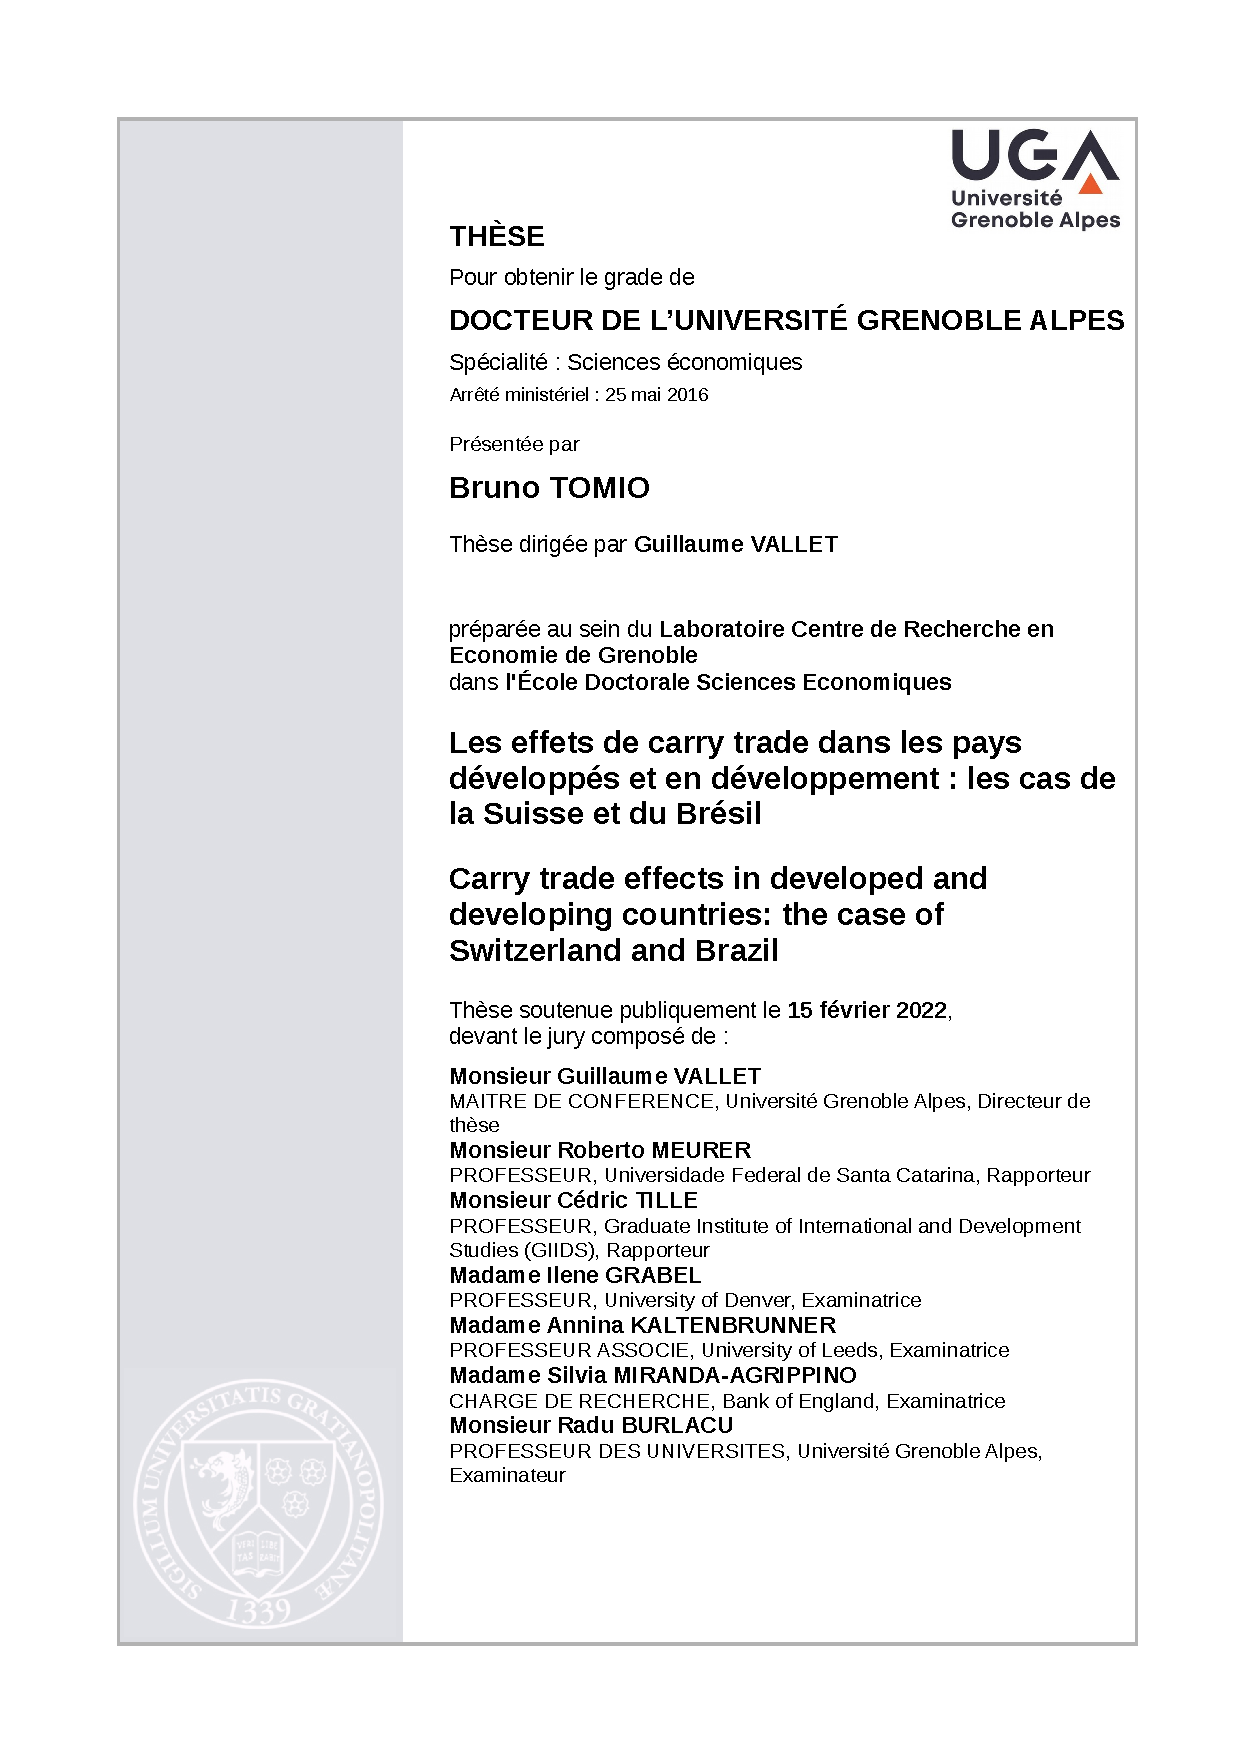
\includepdf[pages=-]{templates/offdoc.pdf}

%%%%% DEDICATION -- If you'd like one, un-comment the following.
\begin{dedication}
  For Maya and Benjamin
\end{dedication}

%%%%% ACKNOWLEDGEMENTS -- Nothing to do here except comment out if you don't want it.
\begin{acknowledgements}
 	I am deeply indebted to Guillaume Vallet for all his constant engagement with this thesis. Words are not enough to express my gratitude for his support, advice, and guidance. His joyful and friendly personality, his enthusiastic passion for research, his willingness to mentor, his jokes to break the tension, and his inspiring intellectual openness have provided invaluable contributions throughout my Ph.D.~experience. Collaborating with him has been a fantastic experience. I hope these collaborations will continue for much longer. In his own words, ``\emph{on ne lâche pas !}'' Above all, thanks a million for your warm friendship. I am very proud to be your first Ph.D.~student to graduate!

  I cannot thank Marc Lavoie, Pierre Berthaud, and Louis-Philippe Rochon enough for pushing me annually during my \emph{comité de suivi individuel} (CSI) meetings. You are and will continue to be, role models that guide me as a researcher. Similarly, Mohamed Amal and Eckhard Hein's guidance during my previous studies were crucial to choosing the academic path. I am very grateful to Sidney Silva's support of my academic career since my undergraduate studies. In advance, I would like to thank the members of my Ph.D.~committee for accepting participation: Roberto Meurer, Cédric Tille, Ilene Grabel, Annina Kaltenbrunner, Silvia Miranda-Agrippino, and Radu Burlacu. Notably, I am deeply grateful to Cédric Tille for his insightful comments, suggestions, and recommendations on an earlier version of the manuscript.

  Many remarkable people helped me during this journey as a Ph.D.~student. In the laboratory Centre de Recherche en Économie de Grenoble (CREG), I own a great deal to Adrien Faudot. During the Minsky Summer Seminar at the Levy Economics Institute of Bard College in 2016, he ``sold'' me the idea to pursue a Ph.D.~in Grenoble. People at CREG have contributed to my journey in Grenoble, namely: Faruk Ülgen, Virgile Chassagnon, Bruno Lamotte, Lindsay Bardou, Solange Amoussou, Catherine Ciesla, Julien Reysz and Hervé Charmettant. Mainly, I am most grateful to the other Ph.D.~students (when I met them), who made the daily routine easier: Marcos Centurión-Vicencio, Ababacar Sadikh Cissé, Hamed Karamoko, Kenneth Ky, Oka Kouadio Denis, Josué Banga, Alassane Diallo, Ibrahim Moussana Alkabous, Gaelle Despierre-Corporon, and Donia Dowidar.

  I am most grateful to the event organizers that made possible vital exchanges to write this thesis. The \texttt{R} community helped me a lot to develop the skills needed to progress in this research. Most importantly, none of this would be possible without the financial support of Universidade de Blumenau (FURB), Coordenação de Aperfeiçoamento de Pessoal de Nível Superior (CAPES), under the Ministry of Education in Brazil, École Doctorale des Sciences Économiques (EDSE) and CREG.

  I also thank my parents for their support of my education. One of my last talks with my grandfather before his passing was about my academic career. While talking about future projects, he mentioned that we would finally have a ``doctor'' in the family. Here we are, \emph{vô}, thank you!

  Finally, I will remember the love and support of Maya, my wife, forever. You are the primary source of all of this. You are more than extraordinary. I will forever thank you for staying next to me. You and Benjamin made this possible. This thesis is dedicated to both of you. \emph{Amo vocês!}

  \begin{flushright}
  Bruno Thiago Tomio \\
  Grenoble, France \\
  25 December 2021
  \end{flushright}
\end{acknowledgements}


%%%%% ABSTRACT -- Nothing to do here except comment out if you don't want it.
\begin{abstract}
	Carry trade is a well-established investment strategy in the world financial market. By profiting from the failure of the uncovered interest rate parity (UIP), speculators position themselves short in a funding currency and long position in a target currency. Two of the main currencies involved in this currency speculation are the Swiss franc and the Brazilian real are investigated in this thesis. The former presents a dual role, funding and safe haven currency, in the actual international monetary system. Regarding the latter, it is a main developing country with a target currency, with a relatively high policy interest rate. Considering these opposed positions, the main question pursued is: how does carry trade impact the real economy activity? After an initial chapter with the research design, this thesis investigates this question in three chapters by proxying the carry trade with the positions data in futures market, published by the United States (U.S.) Commodity Futures Trade Commission (CFTC). Overall, there is evidence that the carry trade impacts the real economy. Nevertheless, the results are different for each currency, which confirms their different position in the currency hierarchy of the actual international monetary system. The general conclusion highlight the need to rethink the role of central banks in the face of the risks associated with the carry trade. These institutions need more domestic cooperation, with macroprudential policies with other national institutions, and international coordination, with more support from global governance institutions.\\

 \noindent \emph{Keywords}: Carry trade; Financialization; Systemic risk; Switzerland; Brazil

 \newpage

 \hypertarget{résumé}{%
 \chapter*{Résumé}\label{résumé}}
 \thispagestyle{empty}

 \adjustmtc
 \markboth{Résumé}{}

 Le carry trade est une stratégie d'investissement bien établie sur le marché financier mondial. En profitant de la non validité de la parité des taux d'intérêt non couverte (UIP), les spéculateurs se positionnent « short » sur une devise de financement et « long » sur une devise cible. Deux des principales devises impliquées dans cette spéculation monétaire, le franc suisse et le real brésilien, sont étudiées dans cette thèse. Le franc suisse présente un double rôle, comme monnaie financement et refuge, dans le système monétaire international actuel. Concernant le real brésilien, il s'agit de la monnaie d'un des principaux pays en développement avec une devise cible, avec un taux d'intérêt directeur relativement élevé. Face à ces positions opposées, la principale question poursuivie est : comment le carry trade impacte-t-il l'économie réelle ? Après un premier chapitre présentant notre conception de la recherche, cette thèse examine cette question en trois chapitres en rapprochant le carry trade des données de positions sur le marché à terme, publiées par la Commodity Futures Trade Commission (CFTC) des États-Unis. Dans l'ensemble, il y a des évidences qui demontrent que le carry trade a un impact sur l'économie réelle. Néanmoins, les résultats sont différents pour chaque devise, ce qui confirme leur position inégale dans la hiérarchie monétaire du système monétaire international actuel. La conclusion générale souligne la nécessité de repenser le rôle des banques centrales face aux risques associés au carry trade. Ces institutions ont besoin de plus de coopération nationale, pour mettre en œuvre des politiques macroprudentielles avec d'autres institutions nationales, et de coordinations internationales, avec plus de soutien des institutions de gouvernance mondiale.\\

 \noindent \emph{Mots-clés}: Carry trade ; Financiarisation ; Risque systémique ; Suisse ; Brésil
\end{abstract}

%%%%% MINI TABLES
% This lays the groundwork for per-chapter, mini tables of contents.  Comment the following line
% (and remove \minitoc from the chapter files) if you don't want this.  Un-comment either of the
% next two lines if you want a per-chapter list of figures or tables.
  \dominitoc % include a mini table of contents

% This aligns the bottom of the text of each page.  It generally makes things look better.
\flushbottom

% This is where the whole-document ToC appears:
\tableofcontents

\listoffigures
	\mtcaddchapter
  	% \mtcaddchapter is needed when adding a non-chapter (but chapter-like) entity to avoid confusing minitoc

% Uncomment to generate a list of tables:
\listoftables
  \mtcaddchapter
%%%%% LIST OF ABBREVIATIONS
% This example includes a list of abbreviations.  Look at text/abbreviations.tex to see how that file is
% formatted.  The template can handle any kind of list though, so this might be a good place for a
% glossary, etc.
% First parameter can be changed eg to "Glossary" or something.
% Second parameter is the max length of bold terms.
\begin{mclistof}{List of Abbreviations}{3cm}

\item[API]

Application programming interface

\item[AUD]

Australian dollar

\item[B3]

Brazil Stock Exchange and Over-the-Counter Market

\item[BCB]

Brazilian Central Bank

\item[BGVAR]

Bayesian global vector autoregressive

\item[BIS]

Bank for International Settlements

\item[BOP/IIP]

IMF's Balance of Payments and International Investment Position Statistics

\item[BRL]

Brazilian real

\item[CAD]

Canadian dollar

\item[CBOE]

Chicago Board Options Exchange

\item[CBSR]

Central bank's social responsibility

\item[CDS]

Credit default swap

\item[CFTC]

Commodity Futures Trading Commission

\item[CHF]

Swiss franc

\item[CIP]

Covered interest rate parity

\item[COT]

Commitments of Traders

\item[CSS]

Cross-currency swaps

\item[DI]

(Foreign) direct investment

\item[ETF]

Exchange traded fund

\item[ETN]

Exchange traded note

\item[EUR]

Euro

\item[FDT]

Foreign exchange daily turnover

\item[FED]

Federal Reserve

\item[Forex]

Foreign exchange

\item[FRED]

Federal Reserve Economic Data

\item[FX]

Foreign exchange

\item[FXAs]

Foreign exchange agreement transactions

\item[GBP]

British pound

\item[GCF]

Global common factor

\item[GFC]

Global financial crisis

\item[GFEVD]

Generalized forecast error variance decomposition

\item[GIRF]

Generalized impulse response function

\item[IFS]

International Financial Statistics

\item[IMF]

International Monetary Fund

\item[JPY]

Japanese yen

\item[LHS]

Left-hand axis

\item[LM]

Lagrange-multiplier

\item[MXN]

Mexican peso

\item[MWald]

Modified Wald (test)

\item[NBFI]

Non-bank financial intermediation

\item[NDFs]

Non-deliverable forwards

\item[NZD]

New Zealand dollar

\item[OECD]

Organisation for Economic Co-operation and Development

\item[OTC]

Over-the-counter

\item[PPP]

Purchasing power parity

\item[RBL]

Russian ruble

\item[RHS]

Right-hand axis

\item[RIP]

Real interest rate parity

\item[SNB]

Swiss National Bank

\item[SSA]

Social structures of accumulation

\item[SVAR]

Structural vector autoregressive

\item[SSVS]

Stochastic search variable selection prior

\item[TFF]

Traders in Financial Futures

\item[TINA]

There is no alternative

\item[UEH]

Unbiased efficiency hypothesis

\item[UEP]

Uncovered equity parity condition

\item[UIP]

Uncovered interest rate parity

\item[UNCTAD]

United Nations Conference on Trade and Development

\item[U.S.]

United States of America

\item[USD]

United States of America dollar

\item[VAR]

Vector autoregressive

\item[VIX]

CBOE Volatility Index

\item[ZLB]

Zero lower bound

\end{mclistof} 


% The Roman pages, like the Roman Empire, must come to its inevitable close.
\end{romanpages}

%%%%% CHAPTERS
% Add or remove any chapters you'd like here, by file name (excluding '.tex'):
\flushbottom

% all your chapters and appendices will appear here
\hypertarget{general-introduction}{%
\chapter*{General introduction}\label{general-introduction}}
\addcontentsline{toc}{chapter}{General introduction}

\adjustmtc
\markboth{Introduction}{}

\noindent When I started working on this thesis at the beginning of 2018, carry trade was a well-established investment strategy. Now, in 2021, we are in a brand new world, where a sort of zero lower bound (ZLB) on interest rate differentials and the popularization of crypto-assets\footnote{\textcite[\text{p.} 65]{stix2021} uses ``the term crypto-asset instead of crypto-currency or virtual-currency because crypto-assets lack the characteristics of conventional currencies (i.e.~with respect to their usability for daily transactions or to provide a stable unit of account).''} is making carry trade less implemented. In my opinion, this is a reaction to the dovish monetary policy implemented around the globe as a response to the COVID-19 crisis\footnote{This crisis is also known as the coronavirus (COVID-19) pandemic. See \textcite{cantu2021} for a database gathering the policy responses to the COVID-19 crisis.}. A report by the \textcite[\text{p.} 12]{committeeontheglobalfinancialsystemcgfs2021} indicates that carry trade ``became less attractive in the intermediate aftermath of the Covid-19 shock.'' In a nutshell, the carry trade activity is very likely to occur with the presence of interest rate differentials between two currencies. Nevertheless, this new puzzle does not make the main research question of this thesis fade away: how does carry trade impact the real economy activity? With the outburst of the 2007-08 global financial crisis (GFC), the carry trade, an ``obscure corner of international finance'' \autocite[ \text{p.} 74]{jorda2012}, has shown its dangers for the real economy. For example, as reported by the press at the beginning of this crisis \autocite{fackler2007}, Japanese individuals faced billionaire losses with leveraged carry trade, making life savings disappear suddenly.

In the classic definition, carry trade is a transaction of borrowing a low interest rate currency (e.g., Swiss franc) to invest in a high interest currency (e.g., Brazilian real). In this thesis, the carry trade instrument is the offshore futures market, where the transaction in the investment date demands taking ``a short position in a funding currency and a long position in the destination currency.'' \autocite[\text{p.} 9]{bankforinternationalsettlements2015} Following closely \textcite{brunnermeier2008}, carry trade is proxied by the positions data in futures market published by the United States (U.S.) Commodity Futures Trade Commission (CFTC). As leveraged investments, their sudden stop contributes to the financial amplification of negative externalities of international capital flows.\footnote{``When a large number of borrowers in an economy experience financial difficulty at the same time and engage in deleveraging, their collective actions lead to asset price declines and exchange rate depreciations, which frequently reduce the value of the assets on borrowers' balance sheets and/or increase the value of their liabilities. As a result, the creditworthiness of borrowers declines further, leading to a feedback loop of further deleveraging, asset price and exchange rate depreciations, and balance sheet effects.'' \autocite[\text{p.} 10]{erten2019}}

In a broader theoretical perspective, real variables are not independent of monetary variables, invalidating the classical dichotomy. Despite its redundancy, money is central in a monetary economy. Moreover, as explained by the monetary circuit, the policy interest rate set by the central bank is the first step to investigate real economic activity \autocite[ \text{p.} 332]{rochon2015}. The initial injection or destruction of money in the system is crucial to understanding the linkages between the carry trade activity and the real economy. With each central bank following its policy objectives, monetary swings almost immediately impact other countries in the current international monetary system.

This has not always been the case. Under the Bretton Woods system (1944-71), ``globally fixed exchange rates against the U.S. dollar tied to the price of gold and capital controls'' \autocite[ \text{p.} 146]{fields2015} created a sort of sandbox for the countries' monetary policy. With capital controls being the norm \autocite{grabel2016}, the negative foreign externality of these policies would take a considerable time to reach other countries, notably developing countries. The end of the Bretton Woods is one of the main cornerstones of the actual globalized financial market. Along with the U.S. dollar imposed as the ``global currency,'' another fundamental characteristic of the current international monetary system is the imposition of deregulation.

Basically, financial deregulation is the lifting of barriers and controls in the financial sector. The main idea behind it has been the promotion of efficient and competitive financial markets \autocite{correa2015}. Hence, by freely flowing worldwide, capital would reach the places where it is most needed. This would be possible due to the capital account openness, with less (or the absence of) capital controls. The new macroeconomic policy framework post-Bretton Woods imposed a ``trilemma'' for all national policymakers, except the United States. As summarized by \textcite[\text{p.} 30]{obstfeld2004}, these policymakers are constrained to two of these three policy goals: ``(i) full freedom of cross-border capital movements; (ii) a fixed exchange rate; and (iii) an independent monetary policy oriented toward domestic objectives.'' With very few exceptions, most countries have chosen goals (i) and (ii) imposing a floating exchange rate regime. With the exponential growth of financial innovations, a ``global financial cycle'' was created, rather imposing a ``dilemma'' for policymakers \autocite{rey2015}. This restricts even further the policy goals for nations, where ``independent monetary policies are possible if and only if the capital account is managed, directly or indirectly, regardless the exchange-rate regime'' \autocite[\text{p.} 21]{rey2015}. Here lies the importance of capital controls in a globally coordinated manner.

With finance displacing production from the core of our economic system, a new type of capitalism has been formed. \textcite{minsky1996} called this new stage of development money manager capitalism. It is a finance-led regime with two main propositions, following \textcite[\text{p.} xii]{aglietta2005}: ``better risk-sharing and greater economic efficiency in the allocation of capital'' and ``Shareholder primacy puts an end to the usurpation of power that characterized `managerial capitalism'. It (re-)establishes the respect of private property -- the linchpin of capitalism.'' \textcite{boyer2011} also highlights this new capitalist regime, \emph{la financiarisation}. Concisely, \textcite[\text{p.} 182]{hein2015} says that the ``combination of the liberalization of national and international financial markets, the introduction of the new financial instruments, changes in corporate governance, and so on, may lead to a dysfunctional increase in finance, which increases instability and hinders investment and economic growth, as has been analyzed in the literature on `financialization' and `finance-dominated capitalist'.''\footnote{Section \ref{twotwo} provides a deeper explanation of financialization.}

Overall, both developed and developing countries followed this path towards more flexibility on international capital movements. Nevertheless, the pace and timing of implementing an open capital account and a floating exchange rate regime were drastically different. On the one hand, developed countries started this process much earlier with a very smooth implementation. On the other hand, developing countries have adhered to financial deregulation without being well developed to be able to. ``This recommendation became a key part of the Washington Consensus\footnote{''The term \emph{Washington Consensus} was coined by \textcite{williamson1990} as a way to codify the economic liberalization policies encouraged by international financial institutions (IFIs) as part of their strategy of structural reforms.''\autocite[\text{p.} 293]{ocampo2004}}; and since the 1980s mainstream economists, the World Bank and the IMF have been advising developing countries to reform their financial systems, i.e.~to reduce government intervention in order to get `interest rates right' \autocites[\text{p.} 169]{worldbank1989,long1991}.'' \autocite[\text{p.} 63]{karwowski2017} The result of this rapid deregulation was the spread of the international financial crisis in several developing countries. Notably, a selective list of the most relevant crashes in the developing world is: Latin America debt crisis (the 1980s), Argentina (early 1980s), Asian crises (1997-98), Russia (1998), Brazil (1999), and Argentina (2001-02). These crises' higher frequency, intensity, and contagion did not hold back financialization. Quite the opposite, financial globalization has been intensified. Consequently, it did not take long to see a developed country in the epicenter of such crises. The GFC that started in the U.S. showed how dysfunctional finance has become, spreading recession worldwide. Indeed, the Emperor has no clothes.

Financial innovations, e.g., credit default swaps and derivatives, were among the main drivers of the GFC. These new financial instruments have been negotiated in the non-bank financial intermediation (NBFI) sector. This sector is ``a broad measure of all non-bank financial entities, and comprising all financial institutions that are not central banks, banks or public financial institutions'' \autocite[\text{p.} 3]{financialstabilityboard2020}. At end-2019, almost half of the financial sector assets was attributable to the NBFI sector, estimated in 200.2 trillion of U.S. dollars \autocite{financialstabilityboard2020}. Carry traders profit from this relatively unregulated sphere of the financial sector. Notably, hedge funds, who are ``large carry players'' \autocite[\text{p.} 75]{gabor2015}, accounted for 2.8\% of the NBFI assets in this period \autocite{financialstabilityboard2020}. Nevertheless, traces of the carry trade activity are also present in other sectors. By occurring mostly off-balance sheet, tracking and measuring carry trade is a puzzle for all, especially central banks and researchers.

The Bank for International Settlements (BIS) Triennial Central Bank Survey provides a comprehensive compilation on global foreign exchange and over-the-counter (OTC), i.e., off-balance sheet, derivatives market. In April 2019, the daily turnover of OTC foreign exchange instruments averaged 6.6 trillion U.S. dollars \autocite{bankforinternationalsettlements2019}. According to Figure \ref{fig:Figure31} in Chapter \ref{three}, this daily turnover exceeds by 40 times the daily amount of world trade in U.S. Dollars in 2019 (in comparison to a ratio of 21 in 1989). Albeit not illustrating the size of the carry trade activity, it shows how much finance is disconnected from the real economy needs. To date, the closest picture of carry trade we may have comes from the positioning data supplied by the U.S. Commodity Futures Trade Commission (CFTC). To better understand the impacts of carry trade in the real economy, we need to use this volume indicator, not the usual calculation of carry trade excess returns or carry-to-risk ratios (expected profitability) that is widely used in the literature.

Recent crises did not discourage the increase in the disconnection between the monetary and real sides of the economy. Nonetheless, central banks work hard to tame the adverse effects of monetary variables on the real economy. Paradoxically, these are the same institutions that are central to this disconnection. In general, the main policy response during these crises was monetary easing or tightening, depending on the circumstances. As a side-effect of the degree of liquidity in global markets, exchange rate volatility has been heavily influenced by speculation with leveraged financial instruments in futures markets. As a result, trade is directly impacted by this change in currency values. This shows how carry trade activity could impact the real economy. Likewise, by being very risky by nature, carry trade reinforces the systemic risk in the global economy.

Price volatility is one of the main drivers of speculation in financial markets. \textcite[\text{p.} 111]{kaldor1976} defines speculation ``as the purchase (or sale) of goods with a view to re-sale (re-purchase) at a later date, where the motive behind such action is the expectation of a change in the relevant prices relatively to the ruling price and not a gain accruing through their use, or any kind of transformation effected in them or their transfer between different markets.'' Thus, rather than entering the forward market to reduce the risk from uncertain future prices, as hedgers do, speculators ``assume the risks'' \autocite[\text{p.} 116]{kaldor1976}. As documented by \textcite{brunnermeier2008}, carry trade is strongly linked to currency crash risk. The sudden unwinding of carry trade positions can systemically spread negative shocks that go far away from the foreign exchange market \autocite{hattori2009}. Being leveraged bets, carry trade is very sensitive to market liquidity and funding, which often cause the unwinding of positions \autocite{brunnermeier2008}. Other global or local events can also trigger this unwind, e.g., the GFC, COVID-19, or future climate crises. Given the size of the transactions related to the carry trade activity, our interconnected financial system amplifies their shock worldwide, increasing the systemic risk.

Global speculators profit from the capital account liberalization widely implemented worldwide. In theory, ``{[}c{]}apital account openness can create more financial sector competition, enable portfolio diversification, and provide finance for current account imbalances.'' \autocite[\text{p.} 3]{gallagher2014} For developed countries, like Switzerland, capital account openness may be significantly beneficial because they have ``reached a certain threshold of institutional capabilities needed to manage its financial sector.'' \autocite[\text{p.} 3]{gallagher2014} Nevertheless, for developing countries like Brazil, free movement of international capital seems to be more associated with financial crises and inequality \autocite{gallagher2014}. Further, after the GFC, \textcite[\text{p.} 2]{gallagher2014a} explain that Brazil attracted carry traders, who profited from ``the high domestic policy rate and the sophistication of the Brazilian financial system''. As a result, there was an ``upward pressure on the exchange rate, which has come with higher commodities prices, leading to what we refer to here as `a financialization of the resource curse'.'' \autocite[\text{p.} 2]{gallagher2014a} Along the same lines, the excessive net flows may impact negatively developing countries in a sort of financial Dutch disease\footnote{``The Dutch disease is a country's chronic exchange rate overvaluation caused by the exploitation of abundant and cheap resources, whose production and export is compatible with a clearly more appreciated exchange rate than the exchange rate that makes internationally competitive the other business enterprises in the tradable sector that use the most modern technology existing worldwide.'' \autocite[\text{p.} 372]{bresser-pereira2013}} \autocite{botta2021}.

In this thesis, carry trade and currency carry trade are used interchangeably. In the financial world, there are many different forms of carry trade.\footnote{See more details in Subsection \ref{twothreeone}.} In fact, they have always been central to our modern financial systems. For example, banks and insurance companies do it. By paying low interest rates on demand deposits, banks gain higher interest rates by making long-term loans. Regarding insurance companies, premiums are paid for the assumed risks \autocite{lee2020}. There is also the equity carry trade, which arises from equity return differentials between countries \autocite{girardin2019}. Additionally, the carry trade is often named after the funding currency, e.g., dollar carry trade or yen carry trade. Some common characteristics among all carry trades are: ``leverage, liquidity provision, short exposure to volatility, and a `sawtooth' return pattern of small, steady profits punctuated by occasional large losses'' \autocite[\text{p.} 3]{lee2020}. In general, carry trade is a market ``anomaly,'' where leverage is used ``to harvest arbitrage profits, a way to buy low and sell high'' \autocite[\text{p.} 83]{mehrling2010}.

Some currencies have been more involved than others in the currency carry trade activity. Notably, yields and financial integration, linked to currency internationalization, are among the main explanatory factors of the carry trade. This thesis focuses on two currencies: Swiss franc (funding currency) and Brazilian real (target currency). Both present strong push factors to be implied in the carry trade activity. Respectively, the former has maintained a very low interest rate, while the former has been implementing a relatively very high policy rate for a long time.\footnote{See Figure \ref{fig:Figure311} for the interest rate differentials between Switzerland and Brazil and the United States. For the U.S. policy rate, check Figure \ref{fig:Figure30}.} Both currencies are internationalized, although to a lesser extent in the case of the Brazilian real. According to the BIS data on turnover of OTC foreign instruments by currency, the Swiss franc ranks 7\textsuperscript{th} in the world, while Brazil ranks 19\textsuperscript{th} (see Table \ref{tab:TableAA21} in Appendix \ref{appendixa2}). Furthermore, the choice is also motivated by the lack of studies on both, especially on Brazil. In addition, the Swiss franc and Brazilian real fit relatively well three out of five attributes for appealing currencies in international markets put forward by \autocite[\text{p.} 3]{cohen2015}: ``financial development, foreign policy ties, {[}\ldots{]} and effective governance (safe management of the currency).'' Economic size and military reach are the two attributes that are questionable for both currencies.

Indeed, yields and currency internationalization are key factors characterize the Swiss franc as a funding currency and the Brazilian real as a target currency. Meanwhile, both currencies present specific characteristics in the context of the carry trade activity. On the one hand, the Swiss National Bank (SNB) was one of the first to implement a flexible exchange rate regime in 1974 \autocite{rossi2015}. Along with the role of supplying global liquidity with its low (or negative) policy interest rate, the Swiss franc is also a crucial safe asset during economic turmoils \autocites[see][]{galati2007,ranaldo2010,guillaumin2012}. As pointed out by \textcite[\text{p.} 178]{baltensperger2017}, there is a ``Swiss interest rate bonus''\footnote{This has not always been the case \autocite[see][]{laurent2014}. The bonus is related to Switzerland's economic development, with ``exceptional political, economic, and monetary stability'' \autocite[\text{p.} 178]{baltensperger2017}.}, which leads ``investors to pay a premium for holding Swiss franc fixed income assets''. Therefore, this dual role for the Swiss franc makes it a fascinating case to study, notably in times of negative policy interest rates. Like Brazil, Switzerland also struggles with the impact of the exchange rate on its trade balance. Nonetheless, it is an entirely different problem related to its appreciation, whether in crisis or not. In September 2011, the SNB shocked financial markets by implementing a peg to the euro \autocite{vallet2014}, which lasted until January 2015. Another innovation implemented by the SNB is the negative policy rate. More importantly, the risk factor mainly drives Swiss franc dynamics, notably in turbulent times \autocite{fink2022}, which highlights its role as a safe haven currency. The dual role (funding and safe haven currency) of the Swiss franc makes it a very interesting case to study in the context of the carry trade activity. In other words, it acts as a funding currency during good times and as a safe haven currency in turbulent periods. Therefore, ``it is not the interest rate spread, as emphasised in the carry trade literature, the most consistent and robust predictor of safe haven status'' \autocite[\text{p.} 57]{habib2012}.

On the other hand, Brazilian real was a major target currency after the 2007-08 global financial crisis. Several factors played a role in this attractiveness: very high policy interest rate (relative to other major currencies), prosperous macroeconomic indicators, and an emerging role in global governance. After a period of hyper inflation and high volatility in interest rates in the 1990s, Brazil opted for inflation targeting in 1999 \autocite{barbosa-filho2009} after the successful launch of the Brazilian real in 1994. This choice aimed to improve the macroeconomic stability of the country, in a context of increasing international openness linked to its status as an emerging country \autocite{artus2004,libanio2010}. In 2010, former Brazilian Treasury Minister Guido Mantega announced: ``We're in the midst of an international currency war, a general weakening of currency. This threatens us because it takes away our competitiveness'' \autocite{financialtimes2010}. This ``currency war'' was an indirect effect of the expansionist monetary policies of the developed countries, which sought to provide liquidity to revive their economies. However, this liquidity also ended up impacting the rest of the world, as well as their own countries \autocite{grabel2018}. Therefore, exchange rates of developed and developing countries were affected, modifying trade patterns artificially. Consequently, economic output was also being impacted, which was the primary concern of the Brazilian government while questioning its currency's very unusual appreciation.

Two points are essential to understand the exchange rate problem that arises from the carry trade activity. First, in the case of the Federal Reserve's response to the GFC, ``the excess liquidity added to U.S. financial markets was then exported through carry trades, using dollar borrowings to invest in higher-yielding assets in emerging economies. There, the inflow of dollars used to buy these countries' assets tended to be mopped up by their central banks in sterilization operations intended to prevent inflation and appreciation of their currencies'' \autocite[\text{p.} 11]{darista2018}. Second, these sterilization operations themselves are also considered carry trade activity \autocite{gabor2015}. Therefore, by pilling up the excess flows as international reserves, central banks of emerging economies worsened the problem by pressuring the exchange rate further. It was ``setting in motion a sorcerer's apprentice scenario'' \autocite[\text{p.} 11]{darista2018}, where emerging economies' central banks fostered more speculative currency activity by trying to defend themselves. Hence, a vicious economic cycle with carry trade as a major driver.

Non-cooperative equilibria result from selfish central banks that focus only on the domestic effects of their monetary policies. The lack of collective good in central banking and deregulated global financial markets foster the carry trade activity. The U.S. monetary policy impacts the world economy, not only the U.S., in the ``global financial cycle'' \autocite{miranda-agrippino2020}. International monetary policy spillovers are also well-documented for other central banks \autocites[e.g.,][ for the European Central Bank]{fratzscher2016}[ for the Bank of England]{schmidt2018}. The ``currency hierarchy'' \autocite{cohen1998,depaula2017} is central to explaining the imbalances generated in the existing international monetary system. According to the \textcite{bankforinternationalsettlements2019}, the U.S. dollar accounted for almost half of the daily turnover of OTC foreign exchange instruments in 2019, while the euro, the Japanese yen, and the British sterling accounted for roughly 60\%. Other countries have to find solutions to this non-cooperative system. Notably, carry trade profits from emerging countries' target currencies with ``high interest rates and profitable exchange rate movements'', which expose the ``international monetary subordination necessary to compensate for these currencies' lower standing in the international currency hierarchy'' \autocite[\text{p.} 183]{bonizzi2020}.

Our current international monetary system is susceptible to shocks, as exposed by the numerous financial crises in the last 40 years. Once again, the world economy is suffering from a global crisis, the COVID-19 crisis. One more time, generalized volatility in the global financial markets and global recession negatively impact people's lives. The exorbitant power of the U.S. dollar is still problematic to the global economy. Having a major currency in the international monetary system was one of the major critiques Keynes made in the debates on the Bretton Woods system, when he rather advocated for a system based on ``currency multilateralism'' \autocite[\text{p.} 25]{keynes1978b}. With a climate crisis very next to our days, finance needs to be revamped to work for people's good, for example, as proposed by the Wall Street Consensus \autocite{gabor2021}.

In a dysfunctional system, anomalies will not cease to develop and perpetuate. It is even worse in a system fostered by selfishness. Following the global recession created by the GFC, the dysfunctional finance present in our current system may lead to even worse crises after several crises of lesser magnitude. This thesis aims to investigate one of the prominent anomalies of this system, the carry trade. The carry trade activity links both monetary and real sides of the economy by speculating with currencies. Hence, it is not only the monetary and financial structures that matter for this financial activity, but also the real economy. The main contribution of this thesis is to provide reproducible empirical evidence to understand better the dynamics of the carry trade activity in Brazil and Switzerland. Moreover, by investigating the political economy of the carry trade, this thesis also aims to contribute to further reflections about our dysfunctional system, not only this anomaly.

The remainder of this thesis is structured as follows. In Chapter \ref{two}, the research design of the thesis is presented. This chapter intends to explore further conceptual and theoretical elements, which could not be developed in the subsequent chapters due to the required length of publishers. In the following, three chapters take the form of academic articles. All three are empirical developments of the research question using the CFTC data as a proxy for carry trade. As highlighted by \textcite[\text{p.} 38]{galati2007}, ``{[}d{]}ata on the net open positions of non-commercial traders in different currency futures traded on the Chicago Mercantile Exchange have been the most widely used measure of carry trade activity in the futures market.'' Chapter \ref{three} investigates the carry trade in developed and developing countries, as published in \textcite{tomio2020}. Next, Chapter \ref{four} analyses the Swiss franc carry trade activity in the context of negative policy interest rates. Lastly, Chapter \ref{five} explores the political economy of carry trade, by confronting the real economy effects of carry trade activity in the current structural power of the international monetary system. The choice to focus on the Swiss franc and Brazilian real also relies on expanding the carry trade literature to other currencies. The Japanese yen is one of the main currencies investigated in this literature. Moreover, Chapter \ref{three} and Chapter \ref{four} are written based on \textcite{nishigaki2007} and \textcite{fong2013}, who investigate the yen carry trade with specific measures of the carry trade proxy. Similarly, Chapter \ref{five} uses the most known measure of the CFTC carry trade proxy in the literature, popularized by \textcite{brunnermeier2008}. Finally, the chapter \protect\hyperlink{general-conclusion}{General conclusion} summarizes the main contributions and discusses future research.

\begin{savequote}
The general economic tone since the mid-sixties has been conducive to
short-run speculation rather than to the long-run capital development of
the economy.
\qauthor{--- Hyman \textcite[\text{p.} 57]{minsky2015}}\end{savequote}



\hypertarget{two}{%
\chapter{Research design}\label{two}}

\minitoc

\hypertarget{twoone}{%
\section{Introduction}\label{twoone}}

\noindent This chapter shows how the research approach in this thesis is designed. Beyond explaining the research methods, the main goal is to provide a clear view of the intended contribution of this thesis. As shown in the chapter \protect\hyperlink{general-introduction}{General introduction}, this thesis questions how developing and developed countries are impacted by the carry trade activity. Notably, two countries are at the center of this research: Brazil and Switzerland. Both countries were not chosen randomly, neither by my Brazilian roots or main research interests. The Brazilian real and the Swiss franc are major target and funding currencies in the carry trade strategy, respectively. In recent economic history, the two have been challengers of the monetary policy rules. For example, after the GFC, the Brazilian government imposed capital controls on portfolio investments \autocite{tomio2011,centralbankofbrazil2013}, and the SNB set a minimum Swiss franc to euro exchange rate \autocite{swissnationalbank2011} and introduced negative policy rates in 2014 \autocite{swissnationalbank2014}.

At the time they were implemented, these policies surprised financial market participants. Another common feature was the willingness to defend the domestic currency from foreign capital excesses. In the highly intertwined financial system we live in, countries lose policy space to tame negative international spillovers. In order to escape TINA (``there is no alternative''), central banks have to innovate to achieve different results from those obtained following the usual rule book supplied by global governance institutions (e.g., International Monetary Fund - IMF). Since there is no global regulation, central banks often act unilaterally to tame the negative impacts of the carry trade activity. Overall, investigating the carry trade effects implies also exploring the current international monetary system.

To clarify the aim and scope of this investigation, the initial sections of this chapter explore the theoretical framework. First, Section \ref{twotwo} looks into the origins and the current state of our financialized economic system. It is a system developed by a process known as financialization. Second, in Section \ref{twothree}, there is the carry trade itself. This speculative investment strategy would not cause harm in a world without financialization. Due to the excesses of global finance, the carry trade spread damage worldwide. This background is essential to understand the next chapters. In the following, the conceptual framework is presented in Section \ref{twofour} based on the main research question.

Additionally, the epistemological approach and the research methodology are adapted to the study of the carry trade. Based on the concepts in the philosophy of science, the epistemology used is rooted in realism, skepticism, empiricism and the principle of parsimony. Basically, using assumptions as close as possible to the real economy (realism/realisticness), the reliability of current knowledge (skepticism) on the carry trade literature is empirically tested (empiricism) in simplified models (the principle of parsimony).

Regarding the research methodology, it is a holistic study using quantitative methods, collecting and analyzing secondary data. In holism, the interdependence of actors and institutions is essential. Consequently, this fits the political economy approach to study the complexity of the carry trade activity. In our current dysfunctional system, power relations go beyond the usual binary rationales (i.e., developed or emerging/developing countries; funding or target currencies) explored in the literature. Though relevant to some extent, such dichotomies do not reflect the complexity of carry trade activities and their power relations.

This implies to focusing on the States, but also on central banks and on private investors of different kinds (dealers/intermediaries, asset managers, leveraged funds, etc.). Being the guardians of the currencies, central banks' non-cooperative actions exemplify this logic of power between States that dictate the carry trade. Monetary policy is ``a peculiar form of economic state power'' \autocite[\text{p.} 242]{braun2020}. In this sense, monetary policy fostered financialization while depending on financial markets to be effectively implemented \autocite{krippner2011,braun2018,braun2020a,walter2020}. The dependence of the monetary authority on financial market actors, whom sought to impose their will, is explored by two types of power in the modern political economy: instrumental power (``lobbying capacity'') and structural power (``the financial sector's central position in the economy'') \autocite[\text{p.} 1]{braun2020a}.

In the same line as the analysis of the relationship between central banking and the shadow banking developed by \textcite{braun2020}, the carry trade activity also implies both infrastructural entanglement and power. With free capital movement worldwide and inflation targeting as the main monetary policy, incentives for the carry trade are created with systematic interest rate differentials. On the one hand, the U.S. monetary policy drives the ``global financial cycle'' \autocite{miranda-agrippino2020}. On the other hand, there are two other types of monetary policy in this context. First, other developed countries with central currencies can independently implement their monetary policy (e.g., Euro area, Switzerland, and Japan). Second, the other peripheric countries must subordinate their monetary policy accordingly to the U.S. or other developed countries. Within the carry trade activity, this subordination means relatively higher interest rates and exchange rate volatility, which are ``necessary to compensate for these currencies' lower standing in the international currency hierarchy'' \autocite[\text{p.} 183]{bonizzi2020}.

This thesis aims to fill a gap in the literature by combining the empirical investigation of the carry trade effects on the real economy with a political economy approach. Concerning the quantitative methods, advanced time-series econometrics is used. The choice for these econometric methods is based on the type of data available to proxy the carry trade activity. Moreover, one of the main features of this thesis design is reproducibility. An online repository\footnote{Accessible on \url{https://github.com/bttomio/UGA_thesisdown}.} is available to reproduce the entire thesis with \texttt{R}. In an effort to foster a more ethical and transparent engagement to research in Economics, all econometric procedures are reproducible on Stata (Chapters \ref{three} and \ref{four}) and \texttt{R} (Chapter \ref{five}).

\hypertarget{twotwo}{%
\section{Financialization}\label{twotwo}}

\noindent Episodes of financial crisis have not ceased to increase after the ``Golden Age'' of capitalism. This capitalist phase comprises the period of the 1950s until the early 1970s, when major capitalist economies exhibited great economic performance (e.g., high growth rates and low inflation and unemployment). The end of this golden phase is linked to the ``stagflation'' of the 1970s. Financial markets deregulation was one of the implemented policies to deal with the dual problem of stagnation and inflation. Consequently, a new phenomenon sprouted with deregulated finance: financialization. In the beginning, in the early 1980s, it was restricted to the United States and the United Kingdom. Nevertheless, it did not take too long to spread worldwide \autocite{hein2015b}. One of the well-known manifestations of the global expansion of this new financialized system is the carry trade activity.

Finance-dominated capitalism \autocite{hein2015c} or financialization is defined, following Epstein's seminal work \autocite*[\text{p.} 3]{epstein2005}, as ``the increasing role of financial motives, financial markets, financial actors and financial institutions in the operation of the domestic and international economies.'' This is a very broad (``macro-level'') definition, which helped to aggregate a significant body of literature and create a research agenda \autocite{mader2020}. Table \ref{tab:Table21} shows other definitions, based on three levels of analysis \autocite{vanderzwan2014}: macro (``the emergence of a new regime of accumulation''), meso (``the ascendency of the shareholder value orientation'') and micro (``the financialization of everyday life'').













\begin{table}[!ht]

\caption{\label{tab:Table21}Main definitions of financialization}
\centering
\resizebox{\linewidth}{!}{
\begin{threeparttable}
\begin{tabular}[t]{l>{\raggedright\arraybackslash}p{8,5cm}l}
\toprule
Author & Definition of financialization & Main level\\
\midrule
\textcite[\text{p.} 174]{krippner2005} & ``a pattern of accumulation in which profits accrue primarily through financial channels rather than through trade and commodity production'' & Macro\\
\textcite[\text{p.} 121]{boyer2000}\(^\bigstar\) & process by which ``all the elements of national demand bear the consequences of the dominance of finance'' & Macro\\
\textcite[\text{p.} 3]{tang2010} & ``process [...] through which commodity prices became more correlated with prices of financial assets and with each other'' & Macro\\
\textcite[\text{p.} 29]{palley2008} & ``(1) elevate the significance of the financial sector relative to the real sector; (2) transfer income from the real sector to the financial sector; and (3) contribute to increased income inequality and wage stagnation'' & Macro\\
\textcite[\text{p.} 149]{aalbers2008} & ``capital switching from the primary, secondary or tertiary circuit to the quaternary circuit of capital [...]; that is, the rise of financial markets not for the facilitation of other markets but for the trade in money, credit, securities, etc.'' & Macro\\
\addlinespace
\textcite[\text{p.} 720]{stockhammer2004} & ``increased activity of non-financial businesses on financial markets, [...] measured by the corresponding income streams'' & Meso\\
\textcite[\text{p.} 104]{froud2000} & ``a new form of competition which involves a change in orientation towards financial results but also a kind of speed up in management work'' & Meso\\
\textcite[\text{p.} 864]{orhangazi2008} & ``designate[s] the changes that have taken place in the relationship between the non-financial corporate sector and financial markets'' & Meso\\
\textcite[\text{p.} 4]{froud2006} & ``changes induced by the rhetoric of shareholder value [which] sets firms and households utopian objectives such as value creation by management intervention for giant firms or security through stock-market saving for households'' & Meso-Micro\\
\textcite[\text{p.} 43]{martin2002} & ``insinuates an orientation toward accounting and risk management into all domains of life'' & Micro\\
\bottomrule
\end{tabular}
\begin{tablenotes}[para]
\item \textit{\footnotesize{Source:}} 
\item \footnotesize{Adapted from \textcite[Table 1.1, \text{p.} 7]{mader2020}. From their table notes: ``Selection based on articles carrying `financialization' or `financialisation' in title, and Google Scholar citations $>$ 500, last accessed Feb. 14, 2019; ${}^\bigstar$derived, no explicit definition of financialization given and does not carry `financialization' in title.''}
\end{tablenotes}
\end{threeparttable}}
\end{table}

More precisely, \textcite[\text{p.} 6]{mader2020} define each of these levels as the following: ``macro-level approaches, which usually focus on the transformation of capitalist accumulation or changes in macroeconomic aggregates and often engage with a state/market-dichotomy in processes of financialization; meso-level analyses, which put (mostly non-financial) corporations center stage and examine issues of ownership and control as well as changing corporate relations with financial markets; and micro-level approaches, which highlight how (mostly) non-elite actors are implicated in a `financialization of daily life,' zooming in on financial practices and rationalities in, for instance, saving and borrowing.''

An analysis of the carry trade using these levels shows that it is inherently connected to financialization. Based on the macro-level approaches, this speculative activity gained (i) ground with the internationalization of financial markets and (ii) monetary magnitude with leverage. At the meso level, speculation by non-financial firms with derivatives is ``rare'' \autocite{bartram2019}. Using a sample of S\&P 500 nonfinancial firms for 1993, \textcite{allayannis2001} show that firms use foreign currency derivatives for hedging purposes rather than speculative opportunities. Nonetheless, \textcite[\text{p.} 741]{bruno2017} find that ``found evidence of divergence between emerging and advanced economy firms, with emerging economy firms being more susceptible to carry trades and the associated surrogate financial intermediation activities.'' Indeed, Brazil provides two recent and notorious examples of the problems generated by this facet of financialization, where non-financial firms seek profits from speculative finance. One of the examples is the Brazilian company Aracruz Celulose, which registered losses of U.S.\$2.13 billion in derivatives in the last quarter of 2008 \autocite{zeidan2013}. Another example is Sadia, one of the biggest Brazilian food producers in 2008. Sadia booked a net loss of approximately U.S.\$ 1 billion in 2008 \autocite{desouzamurcia2017}, by turning itself to speculative investments in currency derivatives during the Brazilian carry trade boom.

\begin{quote}
Talk of ``carry trades'' feels out of place in the context of nonfinancial firms, as carry trades are more commonly associated with financial institutions better equipped to take on financial exposures. However, if the nonfinancial firm comes from an emerging economy with capital controls that restricts cross-border financial transactions, the activities of nonfinancial firms take on greater importance in providing avenues to circumvent capital controls. \autocite[\text{pp.} 704-705]{bruno2017}
\end{quote}

At the micro-level, we may not be far from seeing an increase in ordinary people's pursuit of carry trade investment strategies. The popularization of stock trading with apps like Robinhood and Acorns is an example of the recent developments of financialization of daily life. The dangers of speculative financial activity are increasing, notably when trading is handled as a game. This is the gamification\footnote{By implementing ``game design elements in non-game contexts'' \autocite[\text{p.} 2]{deterding2011}, gamification seeks the mimetism of games/entertainment in other areas. Hence, ``since video games are designed with the primary purpose of entertainment, and since they can demonstrably motivate users to engage with them with unparalleled intensity and duration, game elements should be able to make other, non-game products and services more enjoyable and engaging as well'' \autocite[\text{p.} 1]{deterding2011}.} of finance. As shown by \textcite[\text{p.} 13]{heide2021}, ``With millions of unskilled investors flocking to easy-access smartphone-based brokerages with in-built gamified features, it is perhaps reasonable to be sceptical.'' Therefore, the carry trade strategy may be popularized in further developments of the gamification of financial markets.

In order to better understand the tendencies towards financialization, \textcite{hein2015c} provide a comparative analysis of different theoretical approaches (the French Regulation School, the Social Structures of Accumulation {[}SSA{]} approach, and the contribution by several post-Keynesians authors, with particular emphasis on the long-run views provided by Hyman Minsky's contributions). ``What these approaches have in common is the notion that capitalist development is embedded in social institutions and that there is a kind of interdependence between the set of institutions and economic development, each feeding back on the other.'' \autocite[\text{p.} 7]{hein2015c} While investigating the modern capitalism, each approach describes the period of financialization in a specific manner: (i) ``finance-led growth regime'' \autocite{boyer2000} in the French Regulation School, (ii) ``global neoliberal social structure of accumulation'' \autocite{tabb2010} in the SSA approach, (iii) ``finance-dominated capitalism'' \autocite{hein2012} among post-Keynesians, and (iv) ``money manager capitalism'' for \textcite{minsky1996}.

\textcite{hein2015c} use a four-step pattern to compare these approaches. First, they sketch the common views regarding the basic structures. ``{[}A{]}ll approaches consider `capitalist' (Regulation School, SSA), `monetary production' (post-Keynesians) or `financial' (Minsky) economies to be inherently unstable and argue that these economies require stabilizing social institutions.'' \autocite[\text{p.} 43]{hein2015c} Based on a Marxian interpretation, the Regulation School and the SSA approach point to the class conflict (capital versus labor) in the production and distribution as the root for the instability. For post-Keynesians, based on their approach of the monetary production economy, institutions require ``the need to cope with fundamental uncertainty, to provide stable monetary and financial relations, to constrain distribution conflict, and to stabilize aggregate demand in the short and in the long run.'' \autocite[\text{p.} 43]{hein2015c} For Minsky, institutions are undermined by human behavior in financial economies, where the paradox of stability holds (a stable period in the economy breeds an unstable one). Regarding institutional change, on the one hand, within an endogenous mechanism, the Regulation School, the SSA approach, and Minsky view the collapse of the economic system as a result of its success. On the other hand, for post-Keynesians, ``institutional changes seem to be contingent on exogenous shocks, changing power relations and economic policy failures'' \autocite[\text{p.} 43]{hein2015c}.

Second, \textcite{hein2015c} search for the explanation of the origin of financialization. The collapse of profitability in the ``Fordism'' or the ``regulated capitalist SSA'' are the reasons for the emergence of the financialization for the Regulation School and the SSA approach, respectively. For post-Keynesians, economic policy responses to the increasing inflation rates in the 1970s are related to the collapse of a social bargain/compromise of the period of the ``Golden Age'' (1950s-early 1970s). ``Minsky's approach differs from those previously outlined in that he views the transition towards money manager capitalism rather as a gradual process, driven by the stability of `paternalistic capitalism', and based on his credo `stability breeds instability' by increasing appetite for risk etc.'' \autocite[\text{p.} 44]{hein2015c}

Third, the different approaches present complementarities on their views of financialization's main characteristics and features, rather than fundamental differences \autocite{hein2015c}. ``In particular the Regulation School, the SSA approaches and the post-Keynesian contributions seem to agree that the financialization period is characterized by the deregulation and liberalization of national and international financial markets, goods markets and labour markets, by the reduction of government intervention in the market economy, by a rentier/shareholder--manager coalition dominating labour, by a pronounced shareholder value and short-term profitability orientation of firms at the expense of long-run profitable investments in capital stock, by redistribution of income from wages to broad profits, and among wages from direct labour to managers, and by increasing opportunities of creating household debt for consumption purposes, as well as structural changes in the banking sector through securitization, in particular.'' \autocite[\text{pp.} 44-45]{hein2015c} Minsky's approach is more concentrated on the financial economy, emphasizing the instability created by leverage, speculative and Ponzi financing, and frauds. More fundamentally, whereas Minsky's view claims a stronger role of government and central banks (``rescuer of last resort''), the other approaches characterize ``financialization by downsizing governments'' \autocite[\text{p.} 45]{hein2015c}.

Fourth, \textcite{hein2015c} explore the consequences of financialization for long-run economic and social development. They demonstrate that the approaches of the Regulation School and the SSA ``seem to accept the post-Keynesian argument that, in particular, redistribution at the expense of (lower) wages during the financialization period has caused a major problem for aggregate demand'' \autocite[\text{p.} 45]{hein2015c}. Post-Keynesians emphasize the different macroeconomic regimes\footnote{Regarding Brazil and Switzerland, see \textcite{hartwig2013} and \textcite{tomio2020a}, respectively.} or type of developments under the period of financialization that contribute to ``inequality and global current account imbalances''. Both are identified as ``causes for the worldwide Great Recession\footnote{Occurred between 2007 and 2009 \autocite{maclean2015}.}'' \autocite[\text{p.} 45]{hein2015c} For Minsky, the ``increasing instability potentials'' \autocite[\text{p.} 46]{hein2015c} are essential to understand the possible negative spillovers of financialization on the long-run economic and social development of the world economy.

As a consequence of financialization, the disconnection between the monetary and real sides of the economy is increasing. As demonstrated by \textcite{lane2018}, global external assets as a ratio of world GDP increased significantly from 1995 until 2007. By analyzing the international currency positions over 1990--2012, \textcite[\text{p.} S108]{benetrix2015} find that ``the increase in the scale of international balance sheets (especially for advanced economies) means that a given exchange rate shift can now generate much larger cross-border wealth effects relative to GDP.'' Nevertheless, between 2007 and 2015,

\begin{quote}
the growth in cross-border positions in relation to world GDP has come to a halt, reflecting primarily two factors. The first is much weaker capital flows to and from advanced economies, including financial centers, and in particular diminished cross-border activity by banks in advanced economies, including within the euro area. The second is an increase in the relative weight of emerging economies in global GDP, since these economies have lower ratios of external assets and liabilities to GDP relative to advanced economies. \autocite[\text{p.} 190]{lane2018}
\end{quote}

One way of showing this is to divide the amount negotiated in foreign exchange markets (monetary side) by the amount needed for trade, given by the sum of exports and imports, and foreign direct investment, i.e., productive investment (real side)\footnote{This indicator is similar to the ratios proposed by \textcite{mccauley2011} and Ramos \autocite*{ramos2016,ramos2017}. Nonetheless, the use of the sum of trade and direct investment, as a daily mean, as the denominator in the ratio's equation is a novelty in the literature, to my knowledge.}. This ratio indicates how much the foreign exchange markets are disconnected from the real economy necessity of foreign exchange. Moreover, it also shows the strengthening of financialization in the global foreign exchange market. Paradoxically, the more disconnected they are, the monetary side becomes more harmful to the real side.

Apropos the world economy, Figure \ref{fig:Figure21} illustrates the foreign exchange daily turnover (FDT) and the FDT ratio. The latter is given by dividing FDT by the sum of trade and direct investment. The source for the FDT data is the BIS Triennial Central Bank Survey, which ``is the most comprehensive source of information on the size and structure of global foreign exchange (Forex or FX) and over-the-counter (OTC) derivatives markets'' \autocite[\text{p.} 3]{bankforinternationalsettlements2019}. For the real side variables, data is gathered from the IMF's Balance of Payments and International Investment Position Statistics (BOP/IIP)\footnote{Check Appendix \ref{appendixa1} for further details on the data.}. As shown in Figure \ref{fig:Figure21}, the ratio increased from 12.81 in 1986 to 42.57 in 2019\footnote{Table \ref{tab:TableA11} provides the FDT ratio for several countries in each period.}. There was a rapid increase in the ratio between the mid-1980s and mid-1990s. In the 2000s, the ratio declined quite significantly with a rebound from 2010 onward. The evolution of this ratio shows evidence of the extent of the disconnection from the reality caused by financialization. Moreover, the 2019 ratio demonstrates that the foreign exchange daily turnover exceeded the sum of trade and direct investment by roughly 43 times.




\begin{figure}[!ht]

{\centering 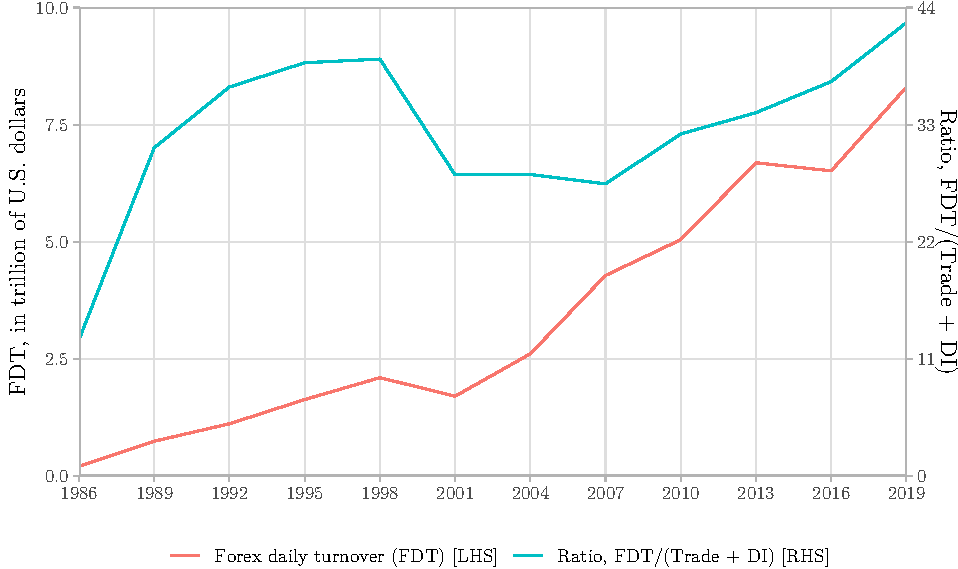
\includegraphics[width=0.99\columnwidth]{_main_files/figure-latex/Figure21-1} 

}

\caption[Forex daily turnover (FDT) and ratio between FDT and the sum of daily trade and direct investment (DI), 1989-2019]{Forex daily turnover (FDT) and ratio between FDT and the sum of daily trade and direct investment (DI), 1989-2019 \\ \scriptsize \textit{Source:} Bank for International Settlements (BIS) for the Forex daily turnover (FDT), using the net-gross basis. International Monetary Fund (IMF) for trade (sum of exports and imports of goods and services in U.S. dollars) and direct investment (sum of net acquisition of financial assets and net incurrence of liabilities in U.S. dollars). \\ \scriptsize \textit{Notes:} Since FDT series are daily means for April, the sum of trade and DI are divided by 252, which is a rule of thumb for the number of trading days in a year \autocite{newyorkstockexchange2021}. See Appendix \ref{appendixa1} for more details. LHS and RHS are the abbreviations for left-hand axis and right-hand axis, respectively.}\label{fig:Figure21}
\end{figure}

The global picture does not capture the specificities of the current international monetary system. By separating emerging/developing and developed economies, the FDT and FDT ratio differences are very significant. In Figure \ref{fig:Figure22}, emerging/developing economies show a volatile FDT ratio. In this same figure, there is the data for this group with the exclusion of Russia. With the exclusion of this outlier, the FDT ratio shows some stability in the period between 2001 and 2019. Similarly, in Figure \ref{fig:Figure23}, the FDT ratio for developed economies is quite stable, after removing the United Kingdom (outlier). Overall, the FDT ratio is much higher in developed countries than in emerging/developing economies by comparing both groups.



\begin{figure}[!ht]

{\centering 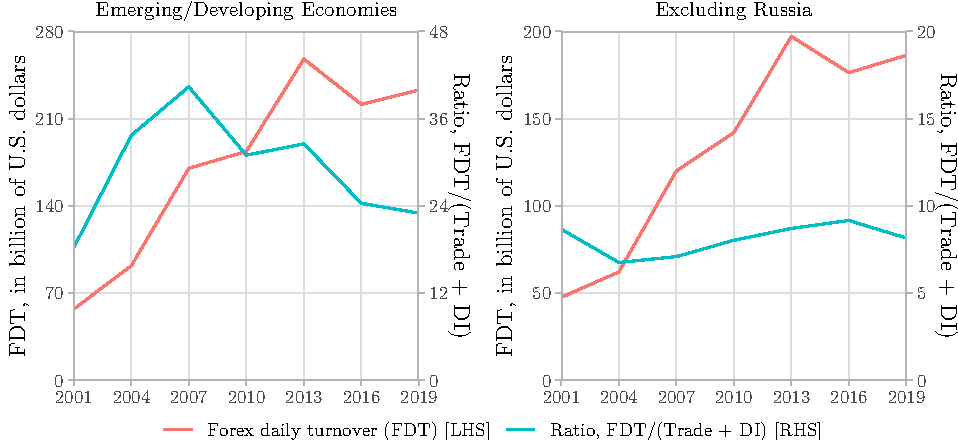
\includegraphics[width=0.99\columnwidth]{_main_files/figure-latex/Figure22-1} 

}

\caption[FDT and ratio between FDT and the sum of daily trade and DI, emerging/developing economies (2001-2019)]{FDT and ratio between FDT and the sum of daily trade and DI, emerging/developing economies (2001-2019) \\ \scriptsize \textit{Countries:} Brazil, Chile, Colombia, Hungary, India, Indonesia, Malaysia, Mexico, Peru, Philippines, Poland, Russia, Saudi Arabia, South Africa, Thailand, and Turkey. \\ \scriptsize \textit{Notes:} See Figure \ref{fig:Figure21} for more details.}\label{fig:Figure22}
\end{figure}

\begin{figure}[!ht]

{\centering 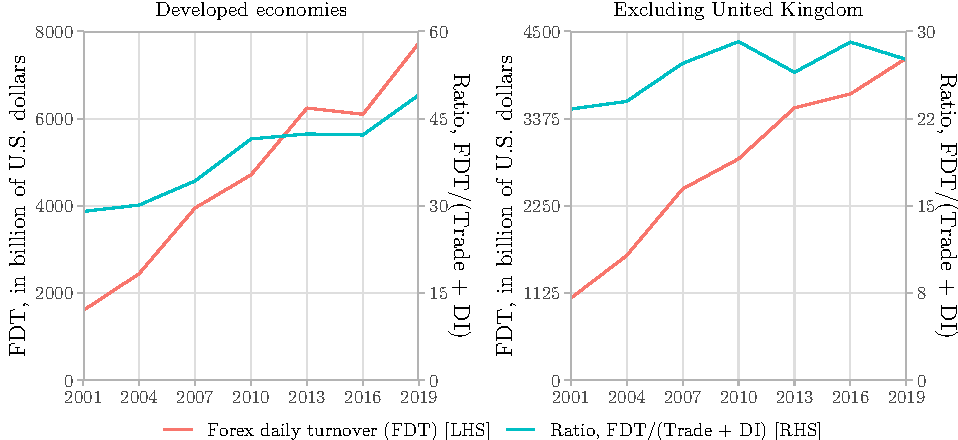
\includegraphics[width=0.99\columnwidth]{_main_files/figure-latex/Figure23-1} 

}

\caption[FDT and ratio between FDT and the sum of daily trade and DI, developed economies (2001-2019)]{FDT and ratio between FDT and the sum of daily trade and DI, developed economies (2001-2019) \\ \scriptsize \textit{Countries:} Australia, Canada, Czech Republic, Denmark, Finland, France, Germany, Greece, Hong Kong SAR, Israel, Italy, Japan, Netherlands, New Zealand, Norway, Portugal, Singapore, Slovakia, South Korea, Spain, Sweden, Switzerland, United Kingdom, and United States. \\ \scriptsize \textit{Notes:} See Figure \ref{fig:Figure21} for more details.}\label{fig:Figure23}
\end{figure}

As far as Brazil and Switzerland are concerned, they follow the same pattern shown by the emerging/developing and developed economies groups, respectively. In 1998, whereas the FDT ratio was 7.7 for Brazil, Switzerland presented a ratio equal to 88.67. In the following surveys, the ratios oscillated significantly for both countries. In the latest figures, the ratio for Brazil is 7.79 against 70.72 in Switzerland.

\begin{figure}[!ht]

{\centering 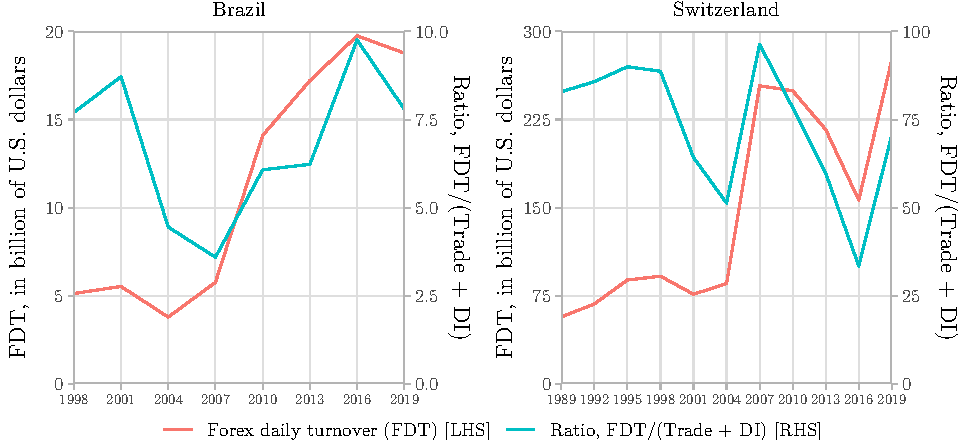
\includegraphics[width=0.99\columnwidth]{_main_files/figure-latex/Figure24-1} 

}

\caption[FDT and ratio between FDT and the sum of daily trade and DI, Brazil (1998-2019) and Switzerland (1989-2019)]{FDT and ratio between FDT and the sum of daily trade and DI, Brazil (1998-2019) and Switzerland (1989-2019) \\ \scriptsize \textit{Notes:} See Figure \ref{fig:Figure21} for more details.}\label{fig:Figure24}
\end{figure}

The BIS Triennial Bank Survey is very useful to show the evolution of financialization in the foreign exchange markets, using the FDT ratios. Additionally, it also shows the differences between emerging/developing and developed economies. While the former is often a group of target currencies in the carry trade strategy, the currencies from the latter group are instead funding or safe haven currencies. Nonetheless, the FDT ratio is not a precise indicator to proxy the carry trade. The next section presents a thorough explanation of the carry trade and its proxies.

Overall, uncoordinated monetary policy is one of the main drivers of the carry trade in our current financialized economic system. As conceptualized by \textcite[\text{p.} 1005]{karwowski2019}, ``{[}t{]}he financialisation of monetary policy {[}\ldots{]} refers to the institutions and policies representing the monetary policy framework (typically with inflation targeting at its heart) and regulating financial markets to maintain financial stability.'' With the policy interest rate being the main tool to control inflation, this framework systematically sets up interest rate differentials on the global financial markets. Therefore, speculative capital can profit from higher yields in one country by borrowing with lower interest rates in another country. In order to curb this type of carry trade, central banks also use sterilization operations to absorb excess foreign capital flows \autocites*[Gabor][]{gabor2010,gabor2010a}. This monetary policy setup is more problematic for emerging/developing countries, which entered into a vicious cycle. According to \textcite{darista2018}, by building up international reserves with the sterilization operations, emerging/developing countries' currencies appreciate, creating more incentive to the carry trade activity. For instance, one action prompted the reaction with continuous feedback while negatively impacting the domestic economy on this cycle.

\hypertarget{twothree}{%
\section{Carry trade}\label{twothree}}

\noindent In the context of this thesis, carry trade is defined as a speculative investment strategy in the foreign exchange market that seeks profits from interest rate differentials and expected exchange rate depreciation and appreciation between countries/currencies. As developed in Subsection \ref{twothreeone}, this definition derives from the research design applied here. Moreover, Subsection \ref{twothreetwo} highlights that the carry trade is a recent subject. As shown in Subsection \ref{twothreethree}, speculators take advantage of the invalidity of one of the major puzzles in international finance theory, the uncovered interest rate parity (UIP). Therefore, it is possible to profit from the carry trade because the expected exchange rate depreciation and appreciation does not offset interest rate differentials. Most importantly, carry trade must not be mistaken as a risk-less market arbitrage\footnote{See more details in Subsection \ref{twothreethree}.}. In order to proxy this speculative investment activity, the volume of future contracts involving speculators is used, as explained in Subsection \ref{twothreefour}. Within the currency pair in the carry trade, one side represents a target currency while the other side is a funding currency. Subsection \ref{twothreefive} shows that this currency classification may change accordingly to the interest rate differentials.

\hypertarget{twothreeone}{%
\subsection{Definition}\label{twothreeone}}

\noindent A precise definition of the carry trade is problematic. As indicated by \textcite[\text{p.} 2]{gagnon2007}: ``{[}t{]}here is no generally accepted definition of what constitutes a carry trade.'' A ``useful'' and comprehensive definition of carry trade would be ``any investment strategy that involves shifting out of low-interest-rate assets and into anything else -- like emerging-market debt, equities, real estate or commodities.'' \autocite[\text{p.} 41]{frankel2008} In this sense, ``carry trade could describe the behavior of any trader seeking to maximize returns on his portfolio''. \autocite[\text{p.} 2]{gagnon2007} Narrowing the definition down, ``carry trade refers to a class of trading strategies that exploit predictable cross-country differences in returns.'' \autocite[\text{p.} 4]{evans2017}

For \textcite[\text{p.} 6]{lee2020}, the ``carry'' is the ``regular stream of income or accounting profits'' produced by the engagement of the trader on this speculative investment strategy. ``The classic finance carry trade takes place in the foreign exchange market, when a trader borrows in a low interest rate currency and invests the proceeds in another, higher-yielding currency.'' \autocite[\text{p.} 6]{lee2020} \textcite[\text{p.} 40]{frankel2008} emphasizes another meaning of the ``carry'' with a simple example: ``In the narrowest sense of the carry trade, the speculator borrows in yen, converts the proceeds to New Zealand dollars, and invests in securities denominated in those dollars. The New Zealand assets are the ones being `carried,' much as a Toyota dealer might carry an inventory of Camrys financed with a bank loan.''

The classic finance carry trade is also known as the \emph{currency} carry trade. Thence, hereafter, carry trade and currency carry trade are used interchangeably. \textcite[\text{p.} 139]{bakshi2013}'s definition goes into this direction: ``Currency carry trade strategies involve borrowing in countries with low interest rates and investing in the currencies of countries that offer high interest rates.'' Otherwise, there is the \emph{equity} carry trade, as investigated by \textcite{cenedese2016}, \textcite{koijen2018} and \textcite{girardin2019}. It is defined as ``{[}t{]}he profit opportunities from selling the low-return domestic equities and buying the high-return foreign ones. As opposed to currency carry trades which target interest rate discrepancies in different countries, equity carry trades track different countries' equity return differentials.'' \autocite[\text{p.} 422]{girardin2019} There are also other examples of carry trades: bond carry trade, yield-curve carry trade, commodity carry trade, credit carry trade and diversified carry trade \autocite[\text{pp.} 187-188]{pedersen2015}.

For the carry trade practitioner, ``{[}c{]}arry is the amount of interest you earn or pay when you own or short a currency.'' \autocite[\text{p.} 42]{donnelly2019} The notion of short and long positioning is essential here. Normally, a trader would go ``short (betting the foreign exchange value will fall) in a low-interest rate currency like the Japanese yen, while simultaneously going long (betting the foreign exchange value will rise) in a high-interest rate currency like the New Zealand dollar.''\footnote{``If you have the opposite position --- long the low-yielder and short the high-yielder --- the interest-rate differential is against you, and it is known as the \emph{cost of carry}.'' \autocite[\text{p.} 191]{brooks2015}} \autocite[\text{p.} 40]{frankel2008} Going into the details, \textcite[\text{p.} 20]{donnelly2019} says that

\begin{quote}
In any financial market, long is the position where you own something, betting that its price will rise. Short is a position where you sell something you dont't own, expecting it to fall. In FX, every currency trade is both a long and a short---you are always selling one currency and buying another.\\
For example, if you go long EURUSD, you own euros and owe dollars, hoping that the euro will go up against the dollar. If you are short EURUSD, you make money when the euro goes down.
\end{quote}

Regarding the yields, they derive from the central bank policy rates. By deriving from the policy rate, other rates are also important: overnight rate and ``2-year, 5-year, or 10-year yields.'' \autocite[\text{p.} 43]{donnelly2019} Nonetheless, the policy rate is the most important, ``since there is a strong relationship between yields all along the curve'' \autocite[\text{p.} 43]{donnelly2019}. Thus, monetary policy is a key factor in understanding the carry trade activity. As highlighted by \textcite[\text{p.} 82]{donnelly2019}, ``{[}i{]}nterest rates are the most important variable driving FX markets much of the time and they tend to be a product of central bank policy.'' More importantly, the influence of main central banks on the carry trade goes beyond the interest rate, as they may exert a ``structural power''\footnote{It is the ``power to shape and mould the structures of production, knowledge, security and credit within which others have no choice but to live if they are to participate in the world market economy'' \autocite[\text{p.} 67]{strange1997}. In this sense, by holding this structural power, the monetary policy (notably, the interest rate policy) applied by main central banks create a restriction for other central banks' monetary policy. This is the fundamental argument of the political economy of the carry trade, which is further developed in Section \ref{twofour} and Chapter \ref{five}.} \autocite{strange1997}.

The simple fact of being a high interest rate currency (i.e., paying a high short-term yield) is not enough to integrate the carry trade in the global financial markets. \textcite[\text{p.} 96]{kritzer2012} highlights some reasons why not every emerging market currency is necessarily a target currency:

\begin{quote}
Emerging market currencies represent the primary targets for carry traders since their corresponding short-term interest rates are perennially high. Their industrialized counterparts, on the flipside, are known for low rates and are better utilized on the short end of the carry trade as funding currencies. Of course, emerging market currencies are also plagued by higher volatility, monetary instability, lower liquidity, and logistical issues related to trading them. The benchmark interest rates of Angola and Kenya, for example, are perennially among the highest in the world, but, for many reasons, their currencies are not well suited for carry trading, let alone normal currency speculation.
\end{quote}

Another key element for this integration is the degree of currency internationalization. \textcite[\text{p.} 9]{kenen2011} defines ``{[}a{]}n international currency is one that is used and held beyond the borders of the issuing country, not merely for transactions with that country's residents, but also, and importantly, for transactions between non-residents.'' As shown by \textcite[\text{p.} 13]{kaltenbrunner2018}'s interviews with foreign exchange market participants in Brazil and London, ``Australian dollar, the Mexican peso, the Turkish lira, the New Zealand dollar and the South African rand (in order of frequency of mentioning)'' are the main emerging market currencies. Table \ref{tab:Table22} presents a list with the emerging market currencies ``most commonly traded by global speculators.'' \autocite[\text{p.} 42]{donnelly2019} Similarly, the same currencies appear on the ranking provided by the \textcite{bankforinternationalsettlements2021b}, using data on the turnover of OTC foreign exchange instruments\footnote{Appendix \ref{appendixa2} provides more details.}.




\begin{table}[!ht]

\caption{\label{tab:Table22}Main emerging market currencies, ranked by liquidity, volume and popularity}
\centering
\resizebox{\linewidth}{!}{
\fontsize{10}{12}\selectfont
\begin{threeparttable}
\begin{tabular}[t]{>{\raggedright\arraybackslash}p{5,75cm}>{\raggedright\arraybackslash}p{4,75cm}>{\raggedright\arraybackslash}p{4,75cm}}
\toprule
Asia & Latin America & Other emerging\\
\midrule
\textbf{China offshore spot (CNH)} & \textbf{Mexican new peso (MXN)} & \textbf{South African rand (ZAR)}\\
 
\textbf{Chinese yuan (renminbi) (CNY)} & \textbf{Brazilian real (BRL)} & \textbf{Turkish lira (TRY)}\\
 
\textbf{Republic of Korean won (KRW)} & \textbf{Chilean peso (CLP)} & Russian ruble (RUB)\\
 
\textbf{Singapore dollar (SGD)} & \textbf{Colombian peso (COP)} & Hungarian forint (HUF)\\
 
Indian rupee (INR) & \textbf{Peruvian new sol (PEN)} & Polish new zloty (PLN)\\
 
Malaysian ringgit (MYR) &  & Israeli shekel (ILS)\\
 
Philippine peso (PHP) &  & Czech koruna (CZK)\\
 
Taiwan dollar (TWD) &  & \\
 
Thai baht (THB) &  & \\
 
Indonesian rupiah (IDR) &  & \\
\bottomrule
\end{tabular}
\begin{tablenotes}[para]
\item \footnotesize{$Source$: Adapted from \textcite[Figure 4.4, \text{p.} 42]{donnelly2019}. \newline \textit{Notes:} The most actively traded currencies are in bold. \textcite[\text{p.} 42]{donnelly2019} clarifies that ``[t]he rankings are my informed but subjective opinion.'' In addition, the ZAR is incorrectly included as 'emerging Europe' in \textcite[Figure 4.4, \text{p.} 42]{donnelly2019}. This was corrected by changing the name to 'other emerging.' }
\end{tablenotes}
\end{threeparttable}}
\end{table}

Regardless of the presence of possible profits with interest rate differentials, the carry trade is not always profitable. The expected exchange rate volatility is also at the core of this speculative activity. As mentioned by \textcite[\text{p.} 185]{pedersen2015}, ``currency moves sometimes reduce the carry trade profit and sometimes add to the profit, and these profits and losses roughly balance out on average.'' There are market adages among traders in this sense. ``Carry trades go up the escalator and down the elevator.'' \autocite[\text{p.} 43]{donnelly2019} Similarly, ``{[}t{]}he carry trade goes up by the stairs and down by the elevator.'' \autocite[\text{p.} 185]{pedersen2015} Or, with an emphasis on the rollover, carry trade is ``known as 'picking up nickels in front of a steam roller.'' \autocite[\text{p.} 43]{donnelly2019}

These sayings are related to the elevated risk of the carry trade. Events of sudden unwind of carry trade operations are known for their colossal impact on exchange rates\footnote{As an illustration of these events, \textcite[\text{p.} 43]{donnelly2019} shows that the ``AUDJPY fall from 107 to 86 in about one month in the Summer of 2007'' and ``the pair dropped all the way from 105.00 to 60.00 in 2008.''} \autocite[i.e., currency crash, as developed by][]{brunnermeier2008}. Overall, globalized financial markets with high capital mobility are a central piece in this complex puzzle. ``Concluding transactions on the forward (or futures) market is simple, flexible, incurs low transaction costs and is available for the general public.'' \autocite[\text{p.} 945]{darvas2009} Another attractive feature of the carry activity to traders is leverage. Therefore, profits can be exponentiated, as well as losses. Notably, with the daily rollover mechanism, leveraged carry trades may ignite panic movements in foreign exchange markets leading to currency crashes.

\hypertarget{twothreetwo}{%
\subsection{Trends on academic and popular interests}\label{twothreetwo}}

\noindent In academic research, the carry trade is a relatively recent subject. According to a search on Google Ngrams\footnote{It is an online search engine (\url{https://books.google.com/ngrams}) to gather and plot data on the frequency of appearances of a specific keyword or phrase on Google Books (\url{https://books.google.com}). It is a useful tool to capture the usage of a term in books from the 1500s until 2019. \textcite{shiller2020} provides an example of its usage by researchers in Economics.}, the usage of the term \emph{carry trade} started increasing after the expansion of research on the \emph{uncovered interest (rate) parity} (UIP)\footnote{See Subsection \ref{twothreethree} for further insights on this relationship. \textcite[\text{p.} 5]{moosa2009} coined a useful term to define the carry trade: ``uncovered interest arbitrage''.} around the 1980s (see Figure \ref{fig:Figure25}). Previously, the presence of \emph{carry trade} on books is mainly related to research on trade, where carry takes the form of the verb\footnote{As an example: ``In its regular publications the chamber finds it to advantage to list trade opportunities and to carry trade advertisements.'' \autocite[\text{p.} 35]{foreigncommercedepartmentchamberofcommerceoftheunitedstates1931}}. Figure \ref{fig:Figure25} shows the 2000s as the period when carry trade gained notoriety, with a peak of uses in 2010. Similarly, in the 2000s, monetary authorities increased their interest on carry trade. For example, the first time the word ``carry trade'' appears in a BIS annual report is in the 69\(^{th}\) report, which comprises the period 1998/99 \autocite{bankforinternationalsettlements1999}. Moreover, one of the seminal papers by central bankers on the subject was published in 2007 \autocite[i.e.,][]{galati2007}.



\begin{figure}[!ht]

{\centering 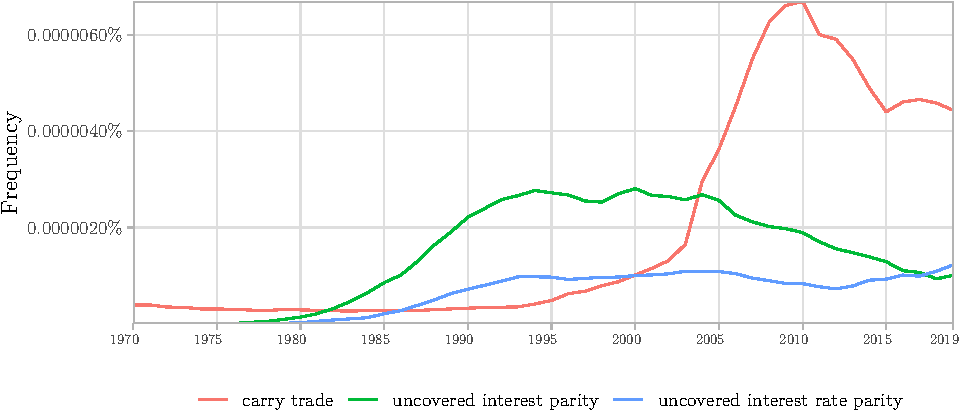
\includegraphics[width=0.99\columnwidth]{_main_files/figure-latex/Figure25-1} 

}

\caption[Frequency of appearance of the keywords \textit{carry trade} and \textit{uncovered interest (rate) parity}, 1970-2019]{Frequency of appearance of the keywords \textit{carry trade} and \textit{uncovered interest (rate) parity}, 1970-2019 \\ \scriptsize \textit{Source:} Data obtained from \textcite{googlebooksngramviewer2021}.}\label{fig:Figure25}
\end{figure}

Although \textcite{doskov2015} find evidence of profitable carry trades dating back to 1901, most authors focus on the period after the collapse of the Bretton Woods System in 1971. More recently, as shown in Figure \ref{fig:Figure26}, academic research on carry trade began exploring specific currencies. The \emph{yen carry trade} firstly appeared in the 1990s. Moreover, ``post 1993 the Japanese yen and Swiss franc have been funding currencies with low interest rates until today, a period covering two decades.'' \autocite[\text{p.} 373]{doskov2015} In the 2000s, the \emph{yen carry trade} peaked its popularity. This is a consequence of some specific characteristics related to the Japanese economy, e.g., interest rates close to zero and ``market actors ranging from Japanese housewives to sophisticated hedge funds'' \autocite[\text{p.} 373]{krugman2018} By spreading globally to other currencies, the terms \emph{currency carry trade} and \emph{dollar carry trade} have been increasing their presence in academic research since the 2000s.



\begin{figure}[!ht]

{\centering 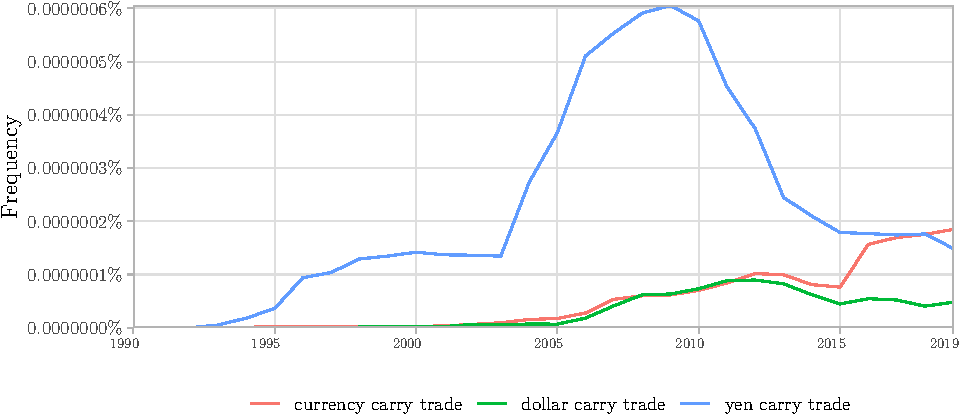
\includegraphics[width=0.99\columnwidth]{_main_files/figure-latex/Figure26-1} 

}

\caption[Frequency of appearance of the keywords \textit{currency carry trade}, \textit{dollar carry trade} and \textit{yen carry trade}, 1990-2019]{Frequency of appearance of the keywords \textit{currency carry trade}, \textit{dollar carry trade} and \textit{yen carry trade}, 1990-2019 \\ \scriptsize \textit{Source:} Data obtained from \textcite{googlebooksngramviewer2021a}.}\label{fig:Figure26}
\end{figure}



According to Google Trends' interest over time\footnote{``Numbers represent search interest relative to the highest point on the chart for the given region and time{[}: \ldots{]} 100 is the peak popularity for the term{[}, \ldots{]} 50 means that the term is half as popular{[}, and \ldots{]} 0 means there was not enough data for this term.'' \autocite{googletrends2021a}}, there are three well-distinguished moments for the number of Web searches for \emph{currency carry trade}, \emph{dollar carry trade} and \emph{yen carry trade} (see Figure \ref{fig:Figure27}). First, the peak in Web searches for \emph{currency carry trade} occurred at the beginning of 2004. After ``the 1990s carry bubble'', the Japanese yen started a new bubble in 2004 with ``very little cost to borrow and very low volatility (thanks to BOJ extreme intervention), with seemingly no risk of appreciating'' \autocite[\text{p.} 26]{lee2020}. The following well-defined moment takes place with the burst of this new carry bubble. Additionally, the number of Web searches for \emph{yen carry trade} culminated in March 2007. With the initial signs of the GFC, the unwind of Japanese yen-funded carry trade explodes. Last but not least, the searches for the term \emph{dollar carry trade} reached their highest point in September 2009. This is a consequence of the funding role assumed by the U.S. dollar, which interest rate was at the record-low level (0.50 bp) after the 1950s \autocite{internationalmonetaryfund2021a}. With currencies altering their role as funding or target throughout time, the interest in the carry trade will persist while the UIP remains invalid.

\begin{figure}[!ht]

{\centering 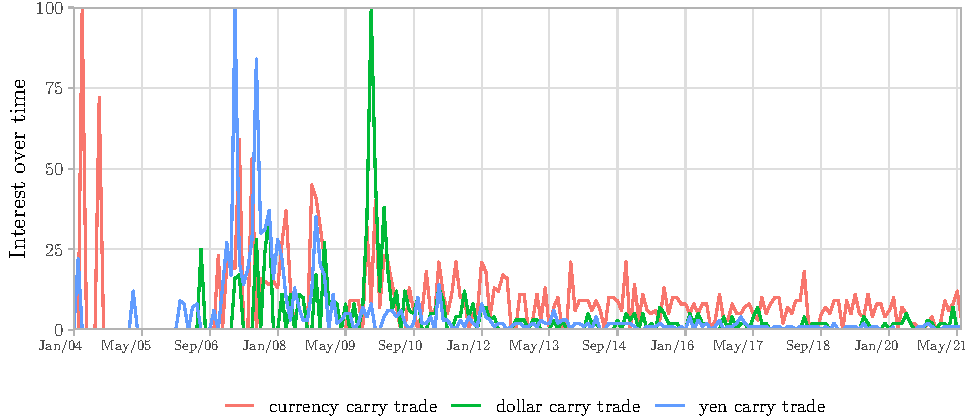
\includegraphics[width=0.99\columnwidth]{_main_files/figure-latex/Figure27-1} 

}

\caption[Search queries on Google Trends for the keywords \textit{currency carry trade}, \textit{dollar carry trade} and \textit{yen carry trade}, Jan/2004-June/2021]{Interest over time for the keywords \textit{currency carry trade}, \textit{dollar carry trade} and \textit{yen carry trade}, Jan/2004-Jun/2021 \\ \scriptsize \textit{Source:} Data obtained from, respectively to each keyword: ``currency carry trade'' \autocite{googletrends2021b}, ``dollar carry trade'' \autocite{googletrends2021c} and ``yen carry trade'' \autocite{googletrends2021d}. \\ \textit{Notes:} As of July 2021, the available data starts in January 2004.}\label{fig:Figure27}
\end{figure}

\hypertarget{twothreethree}{%
\subsection[UIP puzzle]{\texorpdfstring{UIP puzzle\footnote{``The puzzles in economics and finance predominantly take the form of empirical or conceptual anomalies that allegedly remain unresolved and present a challenge to economists. Empirical anomalies, hence puzzles, arise when the implication of a theory is inconsistent with observed economic data; that is, when empirical testing does not support the theory.'' \autocite[\text{p.} 4]{moosa2020}}}{UIP puzzle}}\label{twothreethree}}

\noindent To better understand the carry trade, three terms need to be disentangled: arbitrage, uncovered interest rate parity (UIP) and covered interest rate parity (CIP)\footnote{As developed hereafter, the real interest rate parity (RIP) is intentionally excluded from the interest rate parity theorem, leaving the focus on the UIP and the CIP. Similarly, the purchasing power parity (PPP) theorem is not formulated neither. Both exclusions are not key to understanding the carry trade activity.} In general, there is some confusion on the difference between arbitrage and carry trade. Indeed, both share the same objective: pursuing profit by exploiting price differentials on different markets. In other words, both are trade strategies that simultaneously buy low and sell high. Notably, the difference relies on risk. ``A carry trade is a risk-trading practice \emph{par excellence}.'' \autocite[\text{p.} 74]{gabor2015} ``Arbitrage is the process of buying or selling something in order to exploit a price differential so as to make a riskless profit.'' \autocite[\text{p.} 47]{copeland2014} Although being differentiated by the risk factor, it is common to see both terms used interchangeably by market practitioners. As indicated by \textcite[\text{p.} 92]{copeland2014}, ``{[}t{]}he process of moving capital around so as to exploit uncovered interest rate differentials {[}\ldots{]} is often loosely referred to as arbitrage.'' Theoretically, a carry trade operation cannot be classified as arbitrage. By seeking profits from interest rate differentials and expected exchange rate depreciation and appreciation between two currencies\footnote{As shown in depth in Subsection \ref{twothreefive}, the low and high interest rate currencies are often called funding and investment currencies, respectively.}, it is a risky operation that is rather classified as speculation.

More specifically, for \textcite{dubil2011}, there are two types of arbitrage. First, ``{[}p{]}ure arbitrage is defined as generating riskless profit today by statically or dynamically matching current and future obligations to exactly offset each other, inclusive of incurring known financing costs.'' \autocite[\text{p.} 9]{dubil2011} Considering the spot currency market, this type of ``arbitrage can take a static form, where the trade is put on at the outset and liquidated once at a future date {[}\ldots{]} or a dynamic form, in which the trader commits to a series of steps that guarantee the elimination of all directional market risks and ensure riskless profit upon completion of these steps'' \autocite[\text{p.} 8]{dubil2011}. ``Opportunities for pure arbitrage in today's ultra-sophisticated markets are limited.'' \autocite[\text{p.} 9]{dubil2011} Indeed, a trade that eliminates all risks is very rare. Second, in a new notion, the ``{[}r{]}elative value arbitrage is defined as generating profit today by statically or dynamically matching current and future obligations to nearly offset each other, net of incurring closely estimable financing costs.'' \autocite[\text{p.} 10]{dubil2011} As examples of static and dynamic relative arbitrages, \textcite[\text{p.} 9]{dubil2011} mentions the ``bulk of swap trading'' and a daily dynamically rebalanced ``portfolio of bonds'', respectively. Whereas these two notions of arbitrage take into account price differences of the same item in different periods or markets, speculation is differentiated by dealing with non-substitutable items \autocite[\text{p.} 10]{dubil2011}.

Additionally, one key element to understand the carry trade is the UIP. As stated by \textcite[\text{p.} 1375]{clarida2009}, ``{[}o{]}ne of the enduring puzzles in international finance is the failure of uncovered interest parity (UIP). In a risk-neutral world, the forward exchange rate should be an unbiased predictor of the future spot exchange rate.'' More importantly, if the UIP holds, ``the carry trade would not make any money on average.'' \autocite[\text{p.} 185]{pedersen2015} Algebraically, the UIP may be described as\footnote{See Section 3.1 to 3.5 in \textcite{copeland2014} for a complete mathematical demonstration of both UIP and CIP, including numerical examples.}:
\begin{equation}
r = r^* + \Delta{s}^e
\label{eq:11}
\end{equation}

\noindent where \(r\) and \(r^*\) are the domestic and foreign rates of interest, respectively, and ``\(\Delta{s}\) will be referred to as the rate of depreciation (of the domestic currency) or the rate of increase in the price of foreign currency over the period in question, with {[}\ldots{]} the superscript \(e\) to remind us that in the present case we are concerned with the expected rate of depreciation.'' \autocite[\text{p.} 90]{copeland2014} Moreover, \(\Delta{s}\) is given by the difference between the future and present spot exchange rates\footnote{``Spot FX is simply foreign exchange traded for immediate settlement (i.e., within 1 or 2 days).'' \autocite[\text{p.} 17]{donnelly2019} Equivalently, it ``is the rate used in agreements to exchange one currency for another more or less immediately.'' \autocite[\text{p.} 92]{copeland2014}}.

By definition, the UIP states that ``{[}t{]}he domestic interest rate must be higher (lower) than the foreign interest rate by an amount equal to the expected depreciation (appreciation) of the domestic currency.'' \autocite[\text{p.} 91]{copeland2014} Accordingly, the UIP ``predicts that any differential between a high-interest rate (destination) currency and a low-interest rate (funding) currency at t=0 will be fully offset by the expected change in the exchange rate between t=0 and t=1. In particular, under UIP the exchange rate of the high-interest rate currency would be expected to depreciate so that there are no gains to be made (relative to the low-interest rate currency) from investing in that currency.'' \autocite[\text{p.} 5]{bankforinternationalsettlements2015} Rearranging Equation \eqref{eq:11}, the expected return from the carry trade may be given by:
\begin{equation}
\textit{Expected return} = r - r^* - \Delta{s}^e
\label{eq:12}
\end{equation}

Following Equation \eqref{eq:12}, ``{[}i{]}f UIP holds {[}\ldots{]}, the expected change in the exchange rate would offset the interest rate differential, and the expected return in \eqref{eq:11} would be zero.'' \autocite[\text{p.} 5]{bankforinternationalsettlements2015} If the UIP fails to hold, there is the possibility of positive expected returns. More importantly, the existence of the carry trade derives from the UIP failure. The puzzling invalidity of the UIP is also known as ``the forward-premium puzzle'' \autocites[\text{p.} 448]{lothian2011}[\text{p.} 404]{cieplinski2017}, which ``is precisely what makes the carry trade profitable on average.'' \autocite[\text{p.} 313]{brunnermeier2008} Conversely, carry traders also face the probability of losses. As highlighted by \textcite[\text{p.} 185]{pedersen2015}, ``currency moves sometimes reduce the carry trade profit and sometimes add to the profit''. Usually, ``currency carry trade is characterized by having many small profits and episodic large losses'' \autocite[\text{p.} 185]{pedersen2015}. As highlighted in Subsection \ref{twothreeone}, episodes of rapid unwinding of carry trade positions often lead to great exchange rate volatility. This unexpected volatility can generate huge losses to traders engaged in the carry trade activity within leveraged contracts.

Although the UIP ``has been known among currency traders since the late 19th century'', it was John Maynard Keynes one of the main responsible for its popularization \autocite[\text{p.} 100]{bekaert2017}. As asserted by \textcite[\text{p.} 144]{mehrling2010}, ``{[}a{]}s early as 1913, Keynes used UIP to analyze the foreign exchange relationship between the British pound and the Indian rupee \autocite{keynes1913}. Here is the origin of his later thoughts on forward interest parity \autocite*[\text{p.} 124]{keynes1923}''. Although not a new theory, it is only recently that researchers started testing the validity of the UIP empirically. Overall, ``{[}w{]}hile the uncovered interest rate parity (UIP) hypothesizes that the carry gain due to the interest rate differential is offset by a commensurate depreciation of the investment currency, empirically the reverse holds, namely, the investment currency appreciates a little on average, albeit with a low predictive \(R^2\)'' \autocite[\text{p.} 313]{brunnermeier2008}. Going beyond academia, ``this theory is clearly rejected by the data (as academics have concluded), meaning that the carry trade has historically made money (as macro traders have experienced).'' \autocite[\text{p.} 185]{pedersen2015}

The empirical literature provides compelling evidence of the UIP violation with a wide range of quantitative methods. Basically, the UIP failure indicates that the forward exchange rate is not an unbiased predictor of the future spot exchange rate. Likewise, this violation points out that ``the interest differential is'' not, ``on average, equal to the ex post exchange rate change.'' \autocite[\text{p.} 253]{flood2002} Pioneering the results, there are the seminal papers by \textcite{meese1983} and \textcite{fama1984}, as well as \textcite{hansen1980} and \textcite{cumby1981}. Other examples include, in a non-exhaustive list, \textcite{hodrick1987}, \textcite{cumby1988}, \textcite{bekaert1993}, \textcite{mccallum1994}, \textcite{bekaert1995}, \textcite{dumas1995}, \textcite{engel1996}, \textcite{flood1994}, \textcite{bansal1997}, \textcite{alexius2001}, \textcite{backus2001}, \textcite{flood2002}, \textcite{chaboud2005}, \textcite{chinn2005}, \textcite{brennan2006}, \textcite{sarno2006}, \textcite{bekaert2007}, \textcite{carvalho2009}, \textcite{craighead2010}, \textcite{lee2011}, \textcite{jiang2013}, \textcite{lothian2016}, \textcite{cieplinski2017}, \textcite{adewuyi2019}, \textcite{coulibaly2019}, \textcite{gali2020}, and \textcite{engel2021}. In the real world, the UIP occasionally holds, making it possible to profit from the carry trade.

\textcite[\text{pp.} 1375-1376]{clarida2009} summarizes well, with an emphasis on the carry trade:

\begin{quote}
{[}\ldots{]} papers continue to find that currencies in countries with high interest rates tend on average to appreciate relative to currencies in countries with low interest rates. This stylized fact constitutes the forward rate bias puzzle. The direct implication of the puzzle is that investors can make systematic profits by shorting the low yielding currency and taking a long position in the high yielding currency. This view is often expressed in terms of the apparent profitability of the carry trade, which has become a popular investment strategy in the asset management industry.
\end{quote}

More importantly,

\begin{quote}
According to the principle of uncovered interest rate parity (UIP), the differential of short‐term risk‐free bond yields between two currencies, also known as the forward discount, equals the expected rate of depreciation of the higher yielding currency over the maturity of the interest rate. That said, high interest rate currencies are found to appreciate rather than depreciate over the short‐term \autocites[see, for instance][]{bilson1981,fama1984}. Carry trades exploit the empirical failure of UIP by borrowing at low interest rates in one currency and investing the proceeds into a higher yielding currency. \autocite[\text{p.} 758]{dreher2020}
\end{quote}

While the UIP is established in the spot market, the covered interest rate parity (CIP) involves the forward market\footnote{``The (1-, 3- or 12-month) forward (exchange) rate is the rate that appears in contracts to exchange one currency for another 1, 3 or 12 months in advance of the actual transaction.'' \autocite[\text{p.} 92]{copeland2014} ``FX can also be traded via forwards and futures, which means that the trade is done now but settled at a future date.'' \autocite[\text{p.} 17]{donnelly2019}}. Similarly to the UIP, the CIP states that ``{[}t{]}he domestic interest rate must be higher (lower) than the foreign interest rate by an amount equal to the forward discount (premium) on the domestic currency.'' \autocite[\text{p.} 94]{copeland2014} It is also known as the ``no-arbitrage condition'', where ``{[}t{]}his relationship is an application of the law of one price\footnote{``The Law states that identical goods must have identical prices.'\,' \autocite[\text{p.} 191]{lamont2003}} to financial markets (identical financial assets should produce identical returns after covering the foreign exchange risk).'' \autocite[\text{p.} 18]{moosa2003} Historically, according to \textcite[\text{p.} 919]{du2018}, earlier developments of the CIP are found in \textcite{lotz1889}. Nonetheless, the actual formulation of the CIP has its origins in Keynes' book ``A Tract on Monetary Form'' \autocites[\text{pp.} 115--139]{keynes1923}{keynes1978c}, as mentioned by Lavoie \autocites*[\text{p.} 164]{lavoie2000}[\text{p.} 19]{lavoie2021}, \textcite[\text{p.} 144]{mehrling2010} and \textcite[\text{p.} 100]{bekaert2017}.

Close to Equation \eqref{eq:11}, the CIP is normally formulated as, which is also called the ``academic view'' or ``academic theory'' \autocite[\text{pp.} 19-20]{lavoie2021}:
\begin{equation}
r = r^* + f
\label{eq:13}
\end{equation}

\noindent where \(f\) is the forward premium (discount), defined by the proportion by which the forward exchange rate (\(F\)) ``exceeds (falls below)'' the spot rate (\(S\)) \autocite[\text{p.} 94]{copeland2014}:
\begin{equation}
f = \frac{F}{S} - 1
\label{eq:14}
\end{equation}

Moreover, according to the academic view, as recalled by \textcite[\text{p.} 19]{lavoie2021}, ``{[}c{]}overed interest parity is thus a tendency and is only realised when markets are efficient.''

\begin{quote}
Starting from a situation where equation {[}\eqref{eq:13}{]} holds, assume that speculators now expect the future spot rate {[}\(s^e\){]} to be higher than the present forward rate {[}\(F\){]}: they believe that in the near future the dollar will depreciate relative to the sterling pound more than is indicated by the forward rate. Speculators will sell dollars and buy sterling on the forward exchange market (for instance, they promise to pay \$1.30 for each pound they buy in three-month time, but hope that once they get the pounds they will get back \$1.40 on the spot market at that time). As speculators sell dollars forward, the forward rate of the dollar moves up, opening up an intrinsic premium (or a cross-currency basis), as the covered interest parity condition given by equation {[}\eqref{eq:14}{]} will not hold anymore. This produces a profit opportunity for arbitrageurs, who can gain the intrinsic premium without taking any risk, by acting as a counterparty to the speculators, purchasing dollars forward and selling them on the spot market, thus resorting to covered interest arbitrage. \autocite[\text{p.} 20]{lavoie2021}
\end{quote}

In a similar manner to the UIP, the carry trade activity may also arise from CIP deviations. This is not a surprise given the average daily volume of trading in outright forwards\footnote{``Transactions involving the exchange of two currencies at a rate agreed on the date of the contract for value or delivery (cash settlement) at some time in the future (more than two business days later). This category also includes forward foreign exchange agreement transactions (FXAs), non-deliverable forwards (NDFs) and other forward contracts for differences. Outright forwards are generally not traded on organised exchanges, and their contractual terms are not standardised.'' \autocite[\text{p.} 17]{bankforinternationalsettlements2019}}, which totaled \$999 billion per day in April 2019 \autocite[\text{p.} 6]{bankforinternationalsettlements2019}. ``The principle of covered interest parity states that there should be no arbitrage profit to be had from borrowing in the lower interest rate currency to invest in the higher rate currency while fully hedging the currency risk. {[}\ldots{]} The growth of a currency carry trade means that, at least for those participating in the carry trade, there is an implicit expectation that the higher interest rate currency will not depreciate to the extent of the interest rate differential.'' \autocite[\text{p.} 21]{lee2020} In short, under the CIP violation, ``one can lock in guaranteed profit by borrowing in one currency and lending in another, with exchange risk hedged via forward contract.'' \autocite[\text{p.} 121]{bekaert2017} Most importantly, ``{[}f{]}or carry trade investors, the CIP deviations make the carry trade more profitable on the forward than on the cash markets.'' \autocite[\text{p.} 950]{du2018}

Empirically, the validity of the CIP is equally questioned with the most diverse datasets and quantitative methods. In a comprehensive list, some examples include: \textcite{officer1970}, \textcite{taylor1987}, \textcite{fletcher1996}, \textcite{balke1998}, \textcite{peel2002}, \textcite{moosa2004}, \textcite{sarno2005}, \textcite{akram2008}, \textcite{griffoli2010}, \textcite{fong2010}, \textcite{skinner2011}, \textcite{frenkel2015}, \textcite{borio2016}, \textcite{moosa2017}, \textcite{cieplinski2018}, \textcite{augustin2020}, \textcite{cerutti2021}, \textcite{moessner2021} and \textcite{marcal2021}. In general, the main reasons for the UIP and CIP deviations are related to risk, transaction costs and capital controls \autocite{bekaert2017}, as well as the degree of currency attractiveness \autocite{dupuy2021}.

Notably, \textcite{moosa2017} calls the CIP the ``untestable hypothesis'', following the cambist view. As originally formulated by Lavoie \autocite*{lavoie2000,lavoie2002}, as well as \textcite{smithin2002} and \textcite{harvey2004}, ``{[}t{]}he claim of the so-called cambist view\footnote{It is ``sometimes called the bankers' view or the dealing-room view'' \autocite[\text{p.} 20]{lavoie2021}, as well as the post-Keynesian view \autocite[\text{p.} 473]{moosa2017}. ``The name cambist view arose from the fact that the main features of this variant of Keynes's proposition was first made by a French cambist -- Pierre Prissert \autocite*{prissert1972,prissert1972a}.'' \autocite[\text{p.} 21]{lavoie2021} See a full development in \textcite{lavoie2014} and a revisited version in \textcite{lavoie2021}.} is that the forward exchange rate is the result of a simple arithmetic calculation, and hence that the covered interest parity condition properly defined always holds'' \autocite[\text{p.} 14]{lavoie2021}. Hence, ``{[}t{]}here is indeed no point in testing CIP when it is an identity that represents a mechanical operation and an exact formula used by bankers to calculate the forward rate in practice.'' \autocite[\text{p.} 483]{moosa2017}

Therefore, theoretically, ``{[}p{]}utting together the CIP and UIP relations implies that the forward exchange rate and the expected future spot exchange rate must be equal.'' \autocite[\text{p.} 164]{lavoie2000} This affirmation is based on the relation called ``the forward market unbiasedness hypothesis, or the unbiased efficiency hypothesis (UEH). It says that the forward premium ought to be equal to the change in the exchange rate, or, in other words, that the one-month forward exchange rate obtained today ought to equal the spot rate realized in one month.'' \autocite[\text{p.} 479]{lavoie2014} By relying on unbiasedness\footnote{It ``applies when the (3-, 6- or 12-) month forward rate is equal to the spot rate that the market expects to see prevailing when the contract in question matures.'' \autocite[\text{p.} 100]{copeland2014}} and efficient markets\footnote{They ``are ones where prices fully reflect all the available information. There are, therefore, no unexploited opportunities for profit.'' \autocite[\text{p.} 101]{copeland2014}}, both UIP and CIP are theoretically distant from reality. Following the ``post-Keynesian claim that nominal interest rates are essentially exogenous variables, {[}\ldots{]} equations {[}\eqref{eq:11}{]} and {[}\eqref{eq:13}{]} cannot both be true at the same time.'' \autocite[\text{p.} 479]{lavoie2014} In two empirical works, Moosa \autocite*{moosa2004,moosa2015} ties the forward rate to the contemporaneous spot rate rather than to the future spot rate.

\textcite[\text{pp.} 20-21]{lavoie2021} details further the post-Keynesian approach to the CIP:

\begin{quote}
The forward rate is set so that bank dealers cover their costs, given by the interest rate differential. The main difference with the academic theory is that, in the cambist view, the covered interest parity condition is achieved through the hedging behaviour of banks and not through the arbitrage behaviour of some financial investors. It follows that the verification of the covered interest parity condition has no relationship with whether financial markets are efficient or not. Another difference is that, in the cambist view, sales of the dollar on forward exchange markets have an immediate effect on the spot market, as banks will cover themselves by selling dollars spot. A third difference is that the cambist view implies that covered financial flows have no effect whatsoever on the spot exchange rate or on foreign exchange reserves, in contrast to what is asserted by the academic view, because the bank involved will not take any further action since from its perspective the effect of the forward order cancels that of the spot order. Another implication is that central banks that have the nerves to counter speculation by purchasing their own currency on the forward market will not lose any reserves, provided they renew their position when contracts come due and hence hold on to their position until speculators give up theirs.
\end{quote}

Overall, both UIP and CIP are discredited theoretically and empirically. As summarized by \textcite[\text{p.} 276]{moosa2015}, ``an efficient capital market is characterized by the absence of risk premia and rationality of expectations. However, the empirical evidence against the rationality of expectations in the foreign exchange market is rather strong, whereas the theoretical underpinnings of the hypothesis lack soundness and plausibility.'' Nevertheless, the academic debate over UIP and CIP deviations is far from being settled. Meanwhile, carry traders explore the profit opportunities from these violations in the real world. As emphasized by \textcite[\text{p.} 11]{dubil2011}:

\begin{quote}
Many readers view the \emph{no-arbitrage conditions} found in finance textbooks as strict mathematical constructs. They are not mathematical at all. The equations do not represent the will of God, like gravity or thermodynamics laws in physics. They are ensured by the most basic human characteristic: \emph{greed}. Dealers tirelessly look to discover the violations of no-arbitrage, i.e.~opportunities to buy an item at one price and sell a disguised version of that item for another price. By executing trades to take advantage of the temporary deviations from these paramount rules, they eliminate them by moving prices until money cannot be made and, by extension, the equations are satisfied.
\end{quote}

\hypertarget{twothreefour}{%
\subsection{Proxies}\label{twothreefour}}

\noindent One of the major problems in investigating the carry trade is measurement. By occurring mostly in the OTC markets, there is no public transparency, where ``transactions are executed directly between two parties.'' \autocite[\text{p.} 7]{kritzer2012} With no market maker involved, it is impossible to have a precise measure of the carry trade activity. As ``much of the liquidity in the currency market is in the over‐the‐counter forward market'' \autocite[\text{p.} 321]{brunnermeier2008}, measuring carry trade is very problematic. As emphasized by \textcite[\text{p.} 27]{galati2007}, ``carry trades are notoriously difficult to track in the available data.'' Additionally, ``it is difficult to measure carry-trade activity because the data needed to definitively assess how widely this strategy is used are not available.'' \autocite[\text{p.} 441]{curcuru2011} For policymakers, the problem is even bigger because ``data in the public domain (or even data that are accessible to central banks) generally do not allow direct measurement of carry trades.'' \autocite[\text{p.} 81]{bankforinternationalsettlements2015} Therefore, proxies are needed to measure carry trade activity.

In line with the \textcite[\text{p.} 20]{bankforinternationalsettlements2015}, carry trade indicators may be divided into three types: ``indicators of incentives for carry trades (returns, volatility and related variables)'', ``indicators of market liquidity and of arbitrage opportunities'' and ``indicators of position-taking''. None of these indicators can measure carry trade directly, difficulting the task to understand better how this speculative impact the real economy. Notably, central banks are plainly impacted because ``carry trades raise important policy issues and may pose significant risks'' \autocite[\text{p.} 2]{bankforinternationalsettlements2015}. Regarding academic research, ``there is often focus on the returns from alternative carry trade strategies that can be shown to be profitable or on publicly available data on positions taken in certain markets that are consistent with carry trades.'' \autocite[\text{p.} 2]{bankforinternationalsettlements2015} While carry trade excess returns capture potential profits (\(ex\) \(ante\) approach), we opt to focus on the positioning data (\(ex\) \(post\) approach) because it is closer to the real world. Overall, there is no easy choice.

The first set of indicators is composed of the indicators of incentives or attractiveness for carry trades. Remarkably, this set of indicators is the main used in academic research. Following the \textcite[\text{p.} 20]{bankforinternationalsettlements2015}, carry trade attractiveness may be measured by three approaches: returns, volatility and related variables. First, carry trade returns are the expected profits or losses in a financial strategy of borrowing a low interest rate currency and lending a high interest rate currency. There are also ``carry-trade-generated portfolios of currency excess returns'' \autocite[\text{p.} 214]{berg2018}, with \textcite{lustig2007} and \textcite{cenedese2014} as other examples. Algebraically, similar to Equations \eqref{eq:12} and \eqref{eq:13} in the previous subsection, the carry trade excess return is given by, as adapted from \textcite[Equation (3), \text{p.} 688]{menkhoff2012} and \textcite[Equation (1), \text{p.} 3]{orlov2016}:
\begin{equation}
\textit{Expected return}_i^{t+1} = r_i^{t} - r_t - \Delta{s}_i^{t+1} \approx f_i^{t} - s_i^{t}
\label{eq:15}
\end{equation}

\noindent where, in period \(t\), ``the interest rate differential is approximately equal to the log forward discount under a covered interest parity condition.'' Therefore, \(f_i^{t}\) is the log one-period forward rate in units of foreign currency \(i\) per funding currency in period \(t\) and \(s^i\) is the log spot exchange rate \autocite[\text{p.} 3]{orlov2016}.

Second, regarding risk and volatility, the carry-to-risk ratio is another carry trade proxy. As summarized by \textcite[\text{p.} 439]{curcuru2011}:

\begin{quote}
The carry-to-risk ratio measures the ex-ante, risk-adjusted profitability of a carry-trade position. This measure is based on the interest rate differential that the carry trade will earn, adjusted for the risk of future exchange rate movements that could erase the trade's profits. We measure this risk using the option-implied volatility of the exchange rate. A higher value of the carry-to-risk ratio indicates a greater risk-adjusted ex-ante profitability of a carry trade.
\end{quote}

According to the \textcite[\text{p.} 20]{bankforinternationalsettlements2015}, the carry-to-risk or ``carry-to-vol'' is one of the main indicators used by central banks and market participants. Nevertheless, when interviewing private sector investors, ``there were mixed views about whether it was really an accurate gauge for the attractiveness of carry strategies. One market participant saw the carry-to-risk as largely a lagging indicator, and said that investors should seek carry when volatility is high and declining, not when volatility is low and rising.'' \autocite[\text{p.} 20]{bankforinternationalsettlements2015}

Third, besides the carry trade excess returns and the carry-to-risk ratio, other indicators are monitored by central banks, as elaborated by the \textcite[\text{pp.} 20-21]{bankforinternationalsettlements2015}: (i) ``{[}a{]}lternative time horizons (short, medium and long run)'', (ii) ``{[}a{]}lternative measures of risk and volatility associated with carry trades'', which may ``include implied volatilities, risk reversals, the Vix and the five-year CDS {[}credit default swap{]} sovereign spread (which, in at least one case, is used to adjust the interest rate differential when computing the carry-to-risk ratio)'', (iii) nominal or real effective exchange rate ``as an indicator of whether carry trade gains are at risk. In particular, signs of real exchange rate misalignment could suggest a greater likelihood of a sudden currency crash that could adversely affect the profitability of carry trade positions'', (iv) ``{[}i{]}ndicators for a wider set of markets, both advanced and emerging example, some central banks monitor alternative funding currencies (USD, CHF, CAD, JPY and EUR) or baskets of currencies, or the performance of indices representing carry trade portfolios. Carry trade returns based on implied rates in the offshore NDF or derivatives market may be monitored as well as onshore rates in fixed income markets when there are restrictions or market segmentation'', and (v) ``{[}c{]}ombinations of indicators'' in a joint analysis, where, for example, ``implied volatilities, implied interest rates and risk reversals are monitored daily, and CFTC non-commercial positions weekly.''

The second set of indicators elaborated by the \textcite{bankforinternationalsettlements2015} is composed of indicators of arbitrage opportunities and market liquidity. ``{[}I{]}t may also be useful to estimate the implied interest rates from derivatives markets (possibly offshore) and compare them to interest rates in fixed income markets.'' \autocite[\text{p.} 21]{bankforinternationalsettlements2015} Regarding central banks in Latin America, each central bank has a different approach to monitoring carry trade.

\begin{quote}
The Central Bank of Brazil looks at indicators of dollar liquidity in the Brazilian market and of convertibility risk, respectively the short-term \(cupom cambial\) (derivatives-implied onshore US dollar interest rate), and the onshore/offshore spread implied in USD futures/NDFs offshore. Another example is the Bank of Mexico, which monitors MXN-implied interest rates in MXN (overnight, one and three months and one year). Implied yields are annualised interest rates for the given currency and tenor derived from CIP. In Peru, the Central Reserve Bank of Peru monitors (i) spreads between local currency interest rates and implied rates from the NDF curve; and (ii) the spread between the local currency risk-free yield curve and the cross-currency swaps (CSS) local currency fixed rate curve. \autocite[\text{p.} 21]{bankforinternationalsettlements2015}
\end{quote}

Most importantly, indicators of position-taking are explored in the third set of indicators \autocite{bankforinternationalsettlements2015}. Instead of considering simulated gains or risks of the carry trade activity, positions data reflect real-world behavior. Latin American central banks cite the CFTC data, along with foreign investor holdings of domestic government debt and positions in derivatives markets, as main positions indicators \autocite{bankforinternationalsettlements2015}. Even more important, CFTC provides a public database where investors in several currencies are classified as speculators (i.e., non-commercial traders) on the futures market. Notably, ``{[}a{]} USD/BRL forward contract, for example, is a synthetic carry trade as it has the same payoff as a traditional carry trade that borrows USD, exchanges this for BRL at the prevailing exchange rate, and invests in BRL for the duration of the forward contract.'' \autocite[\text{p.} 31]{avdjiev2011} In order to avoid repetition, see more details about the CFTC data on Subsections \ref{twothreetwo}, \ref{fourtwoone} and \ref{fivetwoone} in Chapters \ref{three}, \ref{four} and \ref{five}, respectively.

Although representing only a small proportion of foreign exchange activity \autocite{galati2007,bankforinternationalsettlements2015}, CFTC data is ``the best publicly available data, and they give a sense of the direction of trade for speculators.'' \autocite[\text{p.} 321]{brunnermeier2008} More specifically, for Brazil, B3 (Brazil Stock Exchange and Over-the-Counter Market)\footnote{Company formed by the integration of the Sao Paulo Stock Exchange (Bolsa de Valores de Sao Paulo) and the Brazilian Mercantile \& Futures Exchange (Bolsa de Mercadorias e Futuros). The latter was previously known as BM\&FBovespa, as referenced, for example, in \textcite{rossi2012} and the \textcite{bankforinternationalsettlements2015}.} data captures a larger proportion of the market where the carry trade normally operates \autocite{bankforinternationalsettlements2015}. For example, \textcite{rossi2012} uses both B3 and CFTC data to investigate the carry trade in Brazil. Nevertheless, B3 only classifies traders between commercial and non-commercial. Therefore, CFTC data is preferable because it classifies different types of traders, with leveraged funds (hedge funds) appearing separately.

There are several measures of the carry trade using CFTC data in the recent literature. One of the precursors is \textcite[\text{p.} 21]{klitgaard2004}, who calculate the ``net foreign currency position of speculators (long contracts in the foreign currency minus short contracts)''. \textcite[\text{p.} 321]{brunnermeier2008} proxies the carry trade as ``the net (long minus short) futures position of noncommercial traders in the foreign currency, expressed as a fraction of total open interest of all traders'', as similarly implemented by \textcite[\text{p.} 26]{klitgaard2004} For example, \textcite{anzuini2012} and \textcite{hutchison2013} use the same approach to calculate the net positions, as well as Chapter \ref{five}. Additionally, as used in Chapter \ref{three}, \textcite{nishigaki2007} divides long positions by short positions to achieve a construct similar to the trade balance ratio (exports divided by imports). More recently, constructs have been developed to extract information of the carry trade activity excluding the U.S. dollar from the currency pair. One approach is based on \textcite{fong2013}, as detailed in Section \ref{fourtwoone}. \textcite{hasselgren2020} develops another approach to make it possible for specific target and funding currencies, given by
\begin{equation}
\textit{Positions}_{t}^\textit{target,funding} = \textit{Net positions}_{t}^\textit{target} - \textit{Net positions}_{t}^\textit{funding}
\label{eq:16}
\end{equation}

Following a similar display as in the \textcite[Graph A7, \text{p.} 36]{bankforinternationalsettlements2015}, Figure \ref{fig:Figure28} presents data for both Swiss franc and Brazilian real\footnote{For the other currencies available on the CFTC data, see Appendix \ref{appendixa3}}. ``Positive net positions indicate that speculators are going long the foreign currency and shorting the U.S. dollar. Conversely, negative net positions indicate that speculators are shorting the foreign currency and investing in the U.S. dollar.'' \autocite[\text{pp.} 438-439]{curcuru2011} It is important to note that ``{[}d{]}ata are available only for positions for which one of the currencies is the U.S. dollar; thus, for example, we have no direct data on positions that are short yen and long Australian dollar.'' \autocite[\text{p.} 439]{curcuru2011} Therefore, in terms of data specificities, there are two main points to consider while analyzing Figure \ref{fig:Figure28}. First, data shows the different roles played by each currency. Overall, while the Swiss franc presents a net short position for several weeks, net long positions are preponderant in the Brazilian real. Second, gaps in the Brazilian data represent a challenge to the empirical analysis.

\begin{figure}[!ht]

{\centering 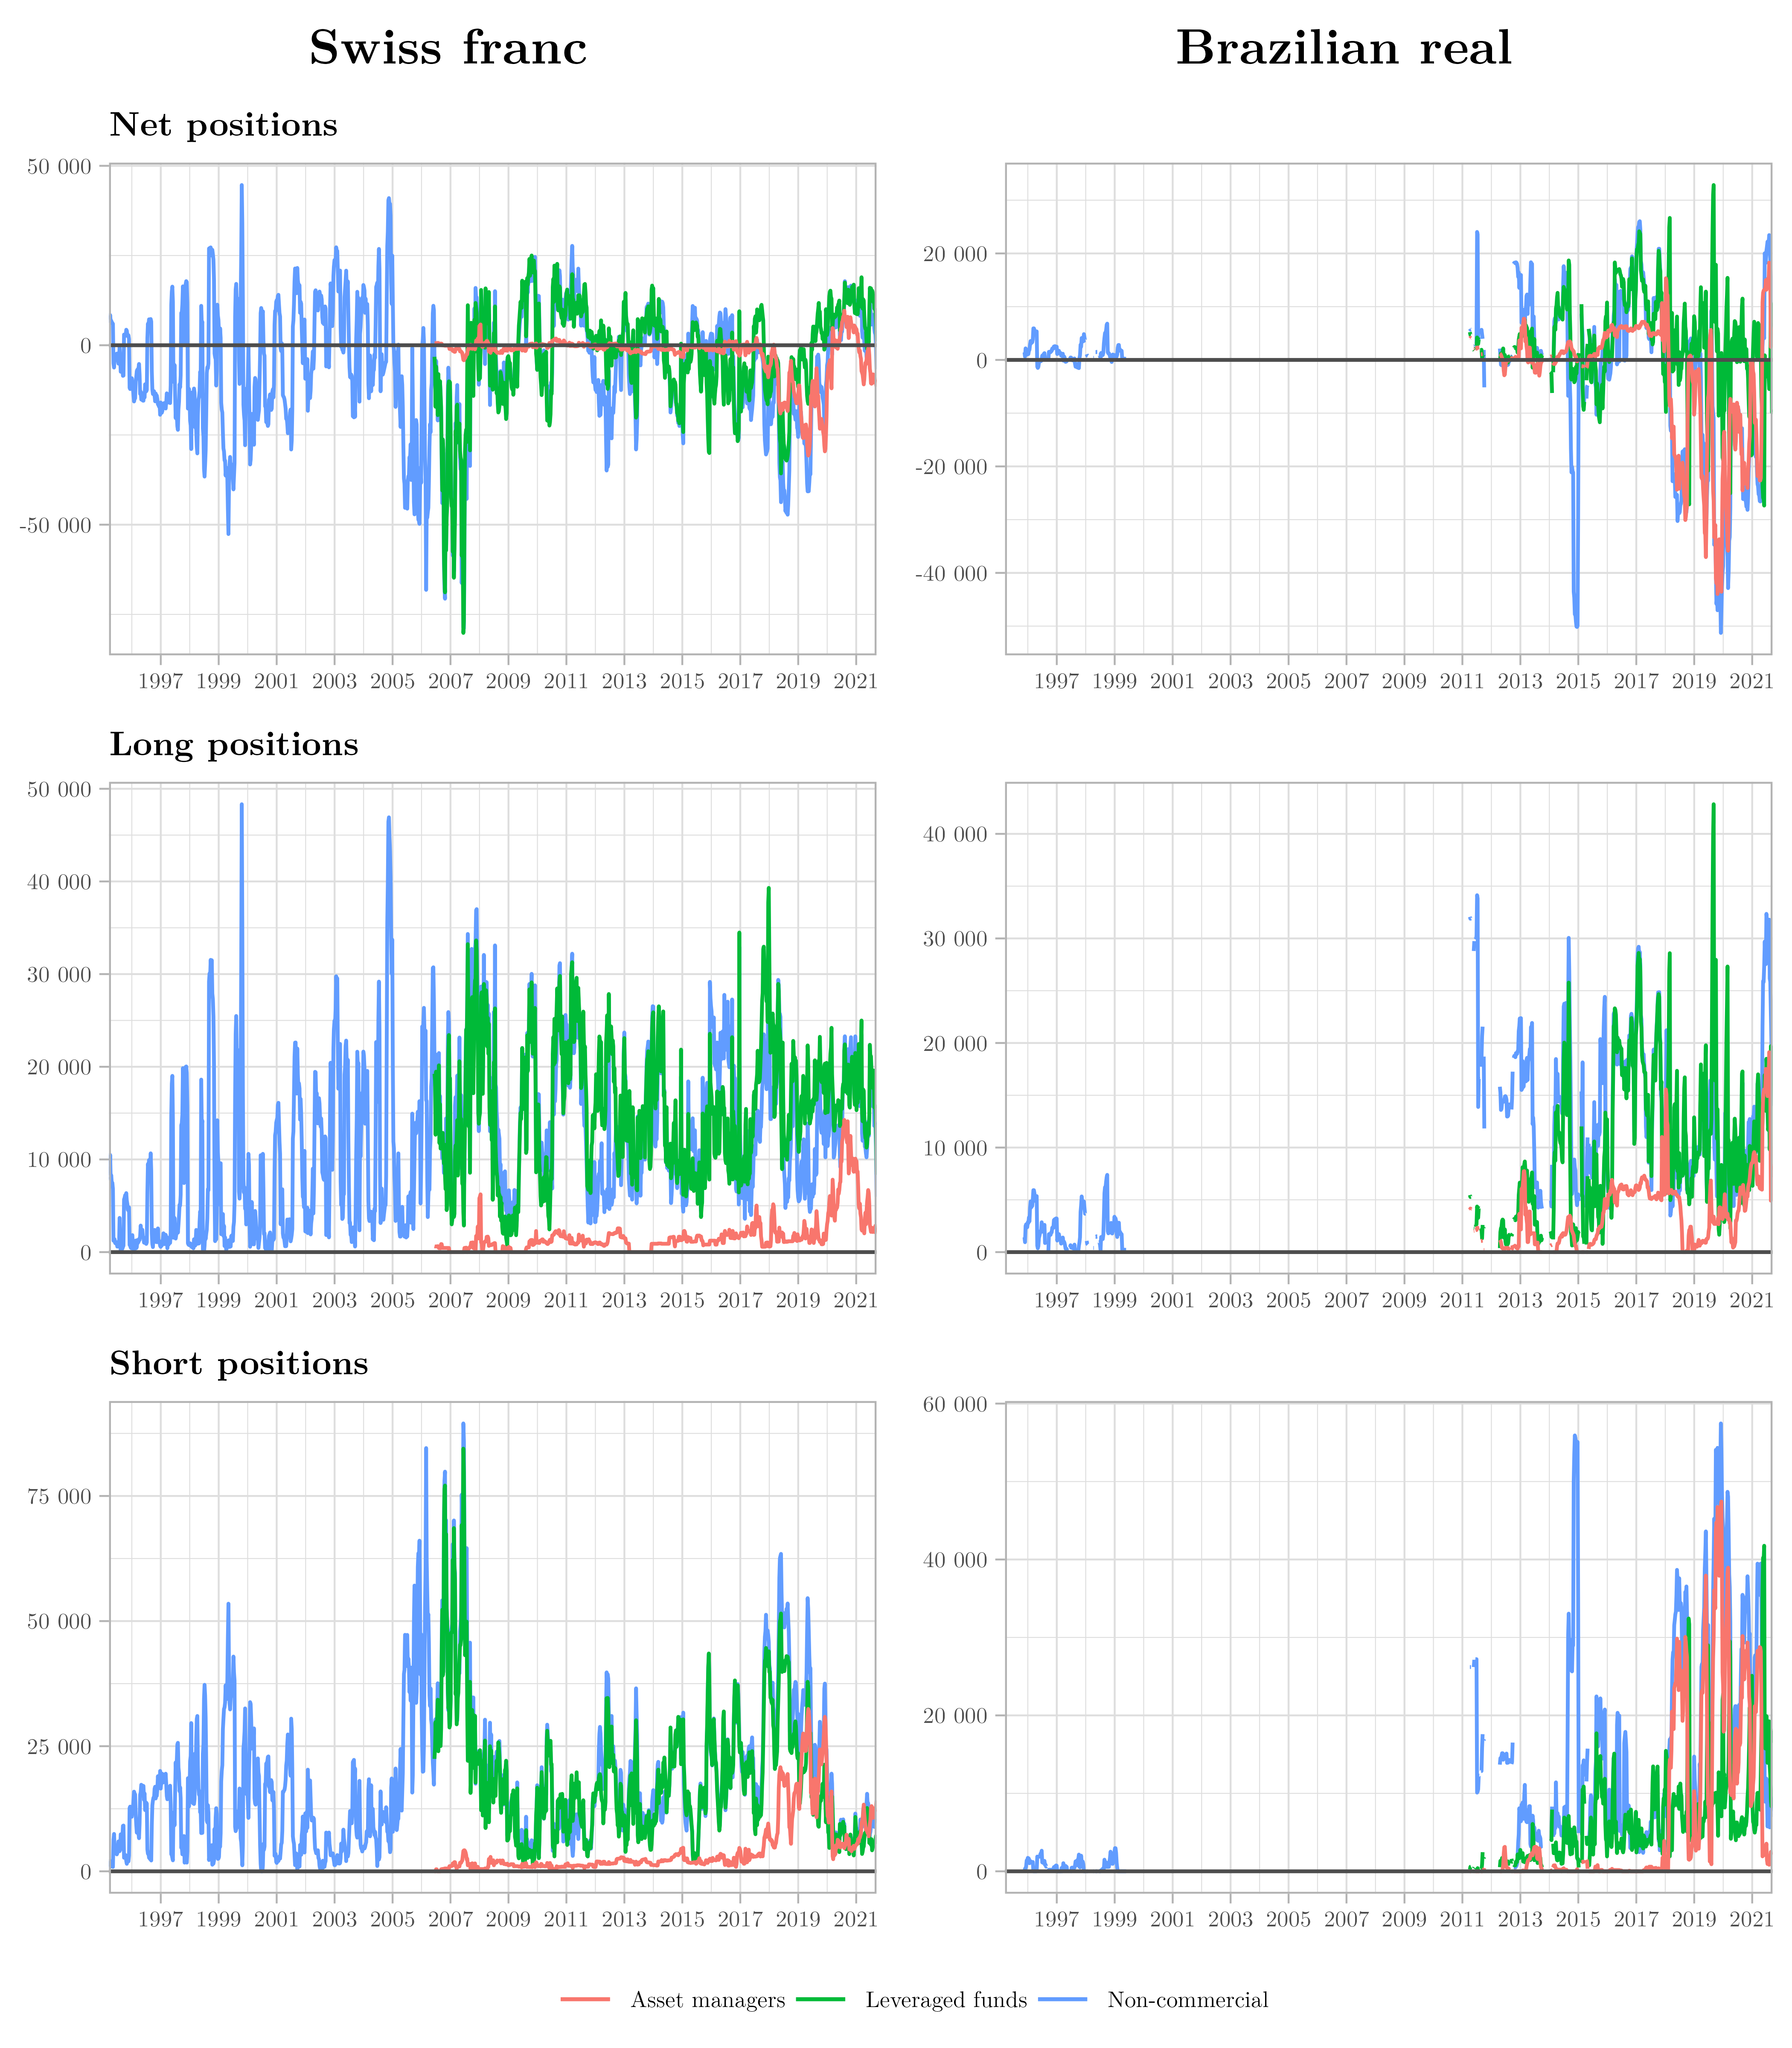
\includegraphics[width=0.99\columnwidth]{figure/GTOG_6} 

}

\caption[Reportable futures and options positions on the Chicago Mercantile Exchange for Swiss franc and Brazilian real, in number of contracts, 1995-03-21 to 2021-09-14]{Reportable futures and options positions on the Chicago Mercantile Exchange for Swiss franc and Brazilian real, in number of contracts, 1995-03-21 to 2021-09-14 \\ \scriptsize \textit{Source:} Commodity Futures Trading Commission (CFTC). \\ \scriptsize \textit{Notes:} Net positions are given by the difference between long and short positions. Regarding the data, two Commitments of Traders (COT) reports are used (with the respective variable between parentheses): Legacy (non-commercial) and Traders in Financial Futures (asset managers and leveraged funds). Regarding the contract size, the values are CHF 125 000 and BRL 100 000, respectively.}\label{fig:Figure28}
\end{figure}

Last but not least, other indicators are mentioned in the literature as carry trade proxies. There is the sentiment index, as calculated by Wang \autocite*{wang2001,wang2004}, which is presented in Appendix \ref{appendixa4}. Alternatively, ``{[}t{]}he BIS international banking statistics can help to highlight activity which may be linked to carry trades, and to investigate more broadly the flow of capital through the international banking system denominated in the main carry trade funding and target currencies.'' \autocite[\text{p.} 32]{galati2007} While analyzing the yen carry trade, \textcite{cecchetti2010} find similarities between CFTC data and their carry trade construct, based mainly on the BIS international banking statistics. For \textcite[\text{p.} 438]{curcuru2011}, ``{[}t{]}he only direct evidence on the carry trade comes from exchange traded funds (ETFs) and exchange traded notes (ETNs), whose returns are linked to carry-trade strategies that involve borrowing in low-yielding currencies and investing in high-yielding currencies. {[}\ldots{]} Unfortunately, ETFs and ETNs are mostly used by retail investors and are unlikely to represent a large percentage of overall carry-trade activity should it exist.''

As explained by \textcite[\text{p.} 46]{kritzer2012},

\begin{quote}
{[}T{]}here are actively managed funds that aim to achieve particular strategies. For example, the Barclays iPath Optimized Currency Carry Exchange Traded Note (ICI) is composed of long positions in high-yielding currencies (those with high local deposit rates) funded with low-yielding (those with cheap borrowing rates) currencies. Rather than seek to profit from currency appreciation, these funds aim to capture the spread from interest rate differentials. The PowerShares DB G 10 Currency Harvest Fund (DBV) employs a similar strategy, aided by leverage. For those with a higher risk tolerance but aversion to hassle, both funds provide a great proxy for the so-called carry trade.
\end{quote}

As ``a popular currency carry index used by practitioners'' \autocite[\text{p.} 376]{doskov2015}, the Deutsche Bank Global Currency Harvest Index ETF joins Barclay's Capital Intelligent Carry Index ETN as the main instruments cited in the academic literature. There are also other carry trade indices in the market (e.g., Citigroup's Beta1 range, Credit Suisse's Rolling Optimised Carry Indices, JP Morgan's IncomeFX and IncomeEM, iSTOXX Europe Carry Factor Net return, SGI FX G10 Carry, Nomura Real Carry USD CIX, GS Short bias TY Vol Carry x1.5, Bloomberg GSAM FX Carry Index and BBG Cumulative FX Carry Index for 8 Emerging Markets). Particularly, there is the recently launched FTSE Climate CaRD Government Bond Index Series, which ``allows sovereign debts investors to lower their portfolio's overall climate risk, while optimizing carry and roll down.'' \autocite{ftserussell2021} Future research on the linkages between carry trade and climate change is needed to tame the negative spillovers of future crises. Notably, policies must take into account the role played by the currency in the carry trade activity.

\hypertarget{twothreefive}{%
\subsection{Currency classification}\label{twothreefive}}

\noindent Within the carry trade strategy, there are always two currencies involved (i.e., currency pair). On the one hand, there is the funding currency, which is also known as the short currency. On the other hand, the target currency completes the currency pair. Also known as long currency, the latter also appears named as ``investment'' currency \autocite[e.g.,][\text{p.} 313]{brunnermeier2008} or ``commodity'' currency \autocite[\text{p.} 80]{rossi2012}. Albeit the simple lexical form, the implementation of the carry trade strategy is complex, complicating the currency classification. Intriguingly, while interviewing market participants, \textcite[\text{p.} 220]{kaltenbrunner2011} indicates that

\begin{quote}
It is interesting to note though that market participants had very different conceptions of carry trades and none of the respondents really thought they were part of this ``notorious'' activity. While hedge funds referred to real money and Japanese investors as the main operators in the carry trade, several real money funds did not think their activity could be described as carry trade due to their longer trading horizon.
\end{quote}

Overall, as previously explained in Subsection \ref{twothreeone}, policy interest rates are key to understanding the role played by each one of the currencies involved in the carry trade. For example, \textcite[\text{p.} 37]{garner2012} explains that ``{[}t{]}he goal of the trade is to benefit from the differential in interest rates, or simply earn more interest on the long currency than is being paid on the short currency.'' Meanwhile, not every currency with a low (high) interest rate is a funding (target) currency. According to \textcite[\text{p.} 87]{mccauley2011}, ``{[}a{]}t given income levels, moreover, currencies with either high or very low yields attract more trading, consistent with their role as target and funding currencies in carry trades.''

Carry trade comprises a small group of currencies, with no established taxonomy to classify them. Even so, two literature strands are essential to understand better the currency classification. First, literature on the monetary hierarchy explores ``the hierarchical structure of the international monetary system.'' \autocite[\text{p.} 187]{depaula2017} At the top, the actual international monetary system is anchored on one key currency: the U.S. dollar. Following \textcite[\text{p.} 52]{deconti2013}, the euro is the second main currency in the global hierarchy, followed by other central currencies (e.g., Japanese yen, British pound, Swiss franc, among others). While the euro reduced its role after the 2007-08 GFC, the U.S. dollar is stronger than ever \autocites[see][]{ilzetzki2019,maggiori2019}. Lastly, there are the peripheral currencies composed of all the other currencies in the world.

This body of literature emphasizes the importance of the political economy to approach the investigation on the carry trade. Both Strange's \autocite*{strange1971} ``political theory of international currencies'' and Cohen's \autocite*{cohen2018} ``currency statecraft'' are crucial in this sense. Furthermore, the debate on the problems generated by this asymmetrical financial system is not recent. As indicated by \textcite[\text{p.} 184]{depaula2017}, one of John Maynard Keynes' main proposals ``for the Bretton Woods Conference was to eliminate the currency hierarchy through the creation of an international currency, the Bancor'' \autocites*[Keynes][]{keynes1978e,keynes1978d}.

Currency internationalization is the second body of literature that helps to characterize currencies in the carry trade better. To measure how internationalized the currency is, one may consider the turnover of OTC foreign exchange instruments provided by the BIS Triennial Survey. The currency hierarchy is presented in Table \ref{tab:TableAA21} (Appendix \ref{appendixa2}) using its latest data available. Similarly, Table \ref{tab:Table22} presents the ranking elaborated by market participants. Regarding developing countries' currencies, the carry trade alone would be a barrier to their full development as an international currency. As summarized by \textcite[\text{p.} 197]{orsi2019},

\begin{quote}
currencies that are solely used for short-term investments, which are essentially speculative, do not improve their position in the currency hierarchy. Therefore, the relationship between currency internationalisation and currency hierarchy is rather non-linear, and also negative when a currency is internationalised only as a short-term investment.
\end{quote}

On the other hand, as a fully developed international currency, the Swiss franc presents several hallmarks:

\begin{quote}
A safe haven currency can serve as the funding currency in carry trades. For example, \textcite{jordan2009} emphasises structural features of Switzerland to explain why the franc serves as a safe haven: the country's political, institutional, social and financial stability, low inflation, confidence in the central bank, comfortable official foreign reserves, high savings and net foreign asset position. For a funding currency in carry trades, however, such structural features matter less than low yields. Japan and Switzerland may have much in common, but it is primarily low yields that have recommended the yen and franc as funding currencies. \autocite[\text{p.} 87]{mccauley2009}
\end{quote}

Centrally, carry trade is about low yields from funding currencies invested in a small group of currencies with higher yields. In our current international financial system, carry opportunities will always be present because different central banks' policies worldwide systematically maintain interest rate differentials. While some central banks are able to pursue the policy rate they wish (funding currencies), periphery central banks (target currencies) are obliged to implement adapted policies greatly considering external conditions. Indeed, great responsibilities follow inseparably from great power (or currency)\footnote{Adapted from \textcite{conventionnationaleparis1793}: ``Les Représentants du peuple se rendront à leur destination, investis de la plus haute confiance et de pouvoirs ilimités. Ils vont déployer un grand caractère. Ils doivent envisager qu'une grande responsabilité est la suite inséparable d'un grand pouvoir. Ce sera à leur énergie, à leur courage, et sur-tout à leur prudence, qu'ils devront leur succès et leur gloire.''}.

The key currency in the existing financial system (U.S. dollar) is a product of the U.S. monetary policy. As ``a driver of the Global Financial Cycle\footnote{It is ``a high degree of co-movement in risky asset prices, capital flows, leverage and financial aggregates around the world'\,' \autocite[\text{p.} 2]{miranda-agrippino2021}. See also \textcite{rey2015}.}'', ``the Federal Reserve monetary policy has important spillovers on global financial markets and liquidity conditions worldwide.'' \autocite[\text{p.} 21]{miranda-agrippino2021} Additionally, it is the ``hegemonic currency'' \autocite{fields2013}, ``which does not mean that the dollar position is unassailable, but at the present moment, there is little evidence of significant changes in the reasonably long foreseeable future.'' \autocite[\text{p.} 547]{vernengo2021} In order to analyze further the currency classification, different periods of monetary policy in the U.S. are taken into account. After the initial date in the CFTC data (2006-06-13), there are five specific monetary periods following U.S. interest rate policy movements. Two periods are characterized by a monetary tightening (MT), i.e., an increase in the U.S. policy rate: MT1 (2006-06-13 to 2007-09-11) and MT2 (2015-12-22 to 2019-07-30). Regarding monetary easing (ME), which comprises a decrease in the policy rate, there are also two periods: ME1 (2007-09-18) and ME2 (2019-08-06). A special period is created to analyze the COVID-19 crisis, where a sharp decrease in the policy interest rate occurred: COVID-19 (2020-03-17 to 2021-09-21). These ups and downs are illustrated in Figure \ref{fig:Figure30}.

\begin{figure}[!ht]

{\centering 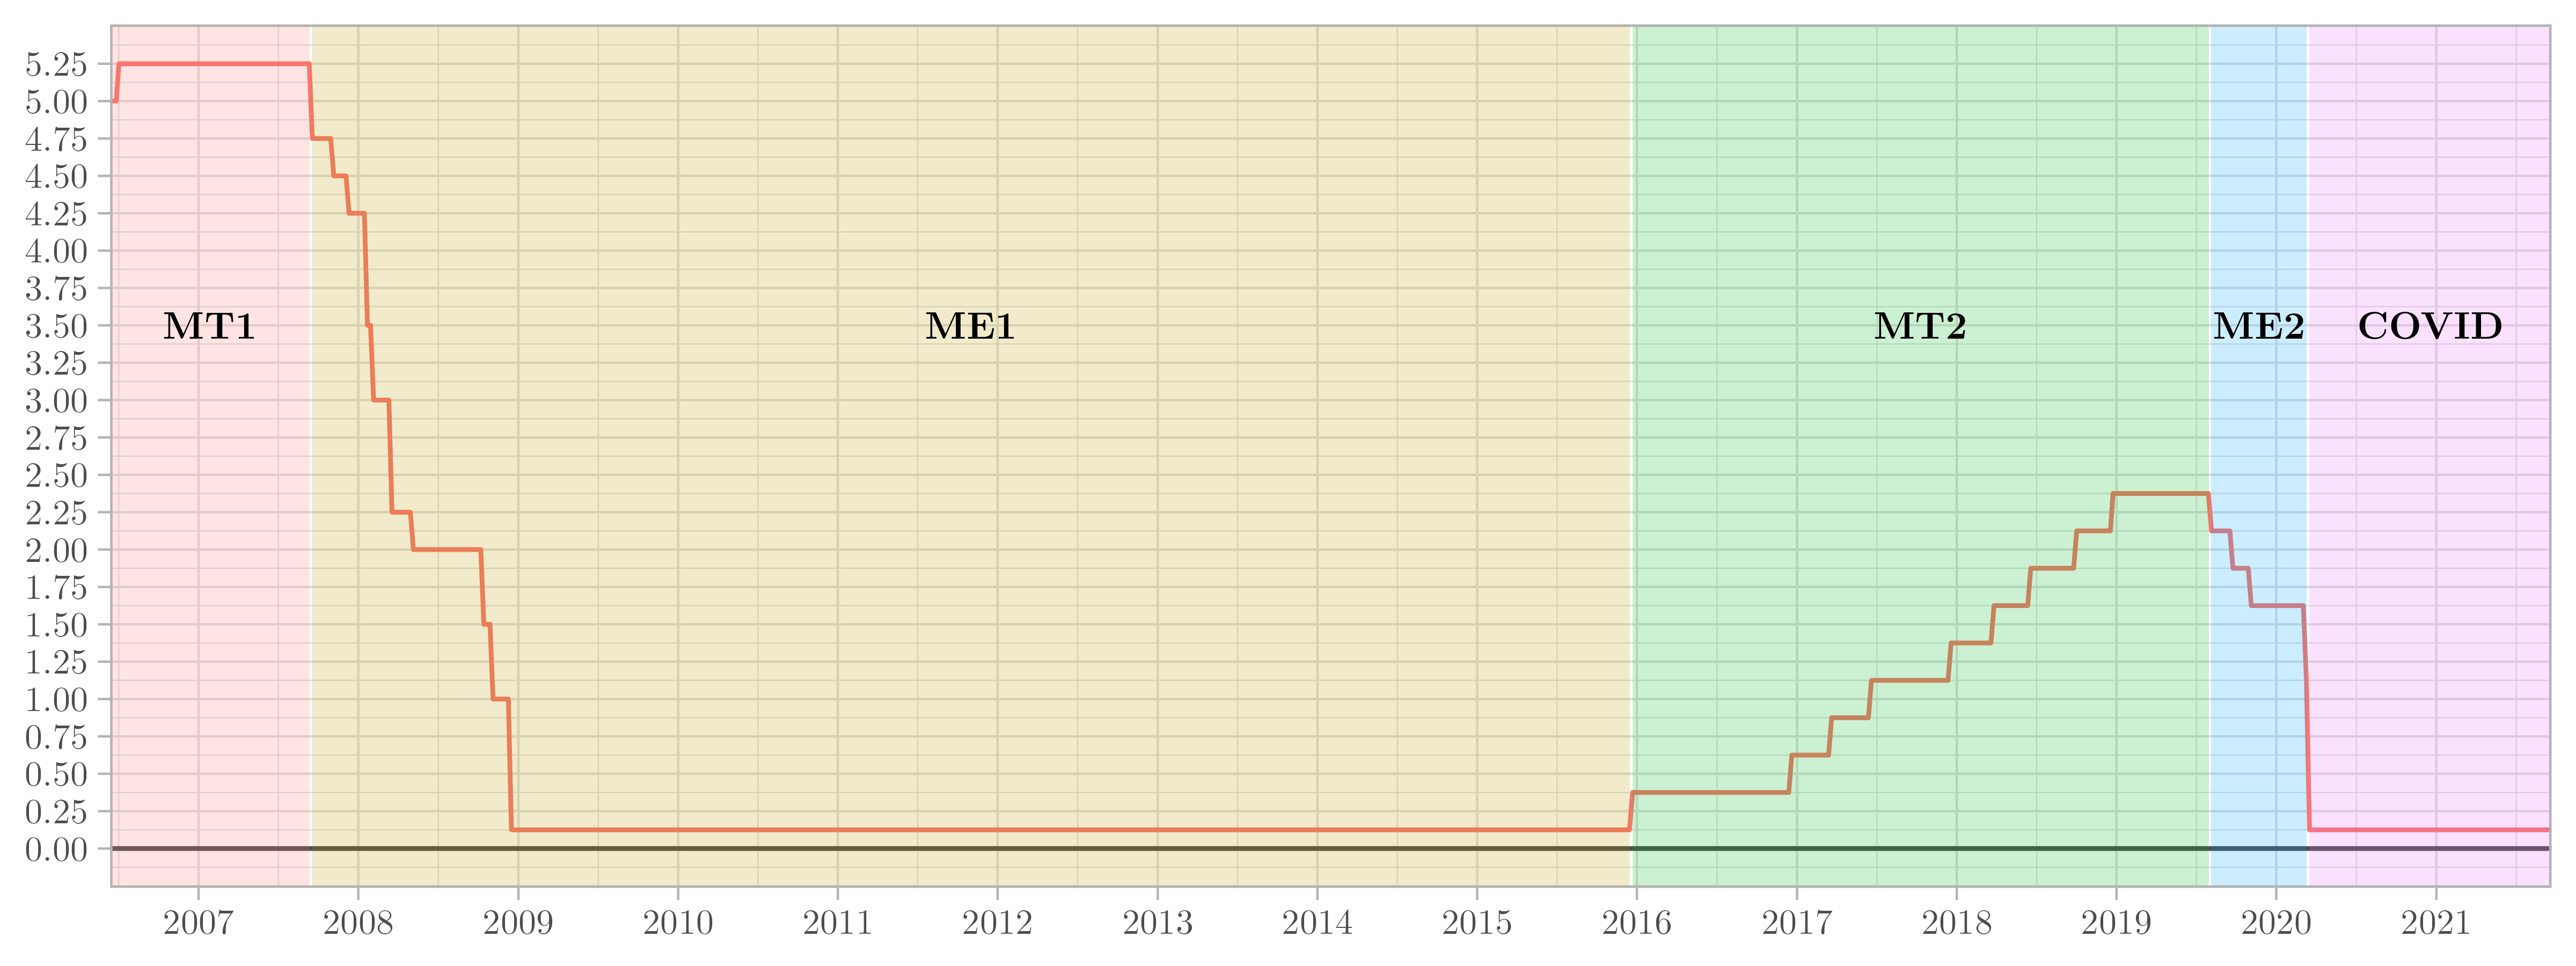
\includegraphics[width=0.99\columnwidth]{figure/USMONPOL} 

}

\caption[Policy interest rate in the U.S., 2006-06-13 to 2021-09-21]{Policy interest rate in the United States, 2006-06-13 to 2021-09-21 \\ \scriptsize \textit{Source:} Bank for International Settlements (BIS).}\label{fig:Figure30}
\end{figure}

Figure \ref{fig:Figure311} displays the interest rate differentials between Switzerland and Brazil and the United States. Globally, a negative value represents the behavior of a funding currency, while positive values are expected for a target currency. Even if Switzerland has a period of positive values, it does not necessarily mean the Swiss franc acted as a target in the carry trade. Still, it is possible because the incentives (i.e., yields) were present (2008-03-18 to 2008-11-18 and 2008-12-16 to 2011-08-02). Another deviance in this figure is the Brazilian real during the COVID-19 period. It seems it reached a sort of bound (ZLB) on interest rate differentials making it oddly unattractive for carry trade in this period.

\begin{figure}[!ht]

{\centering 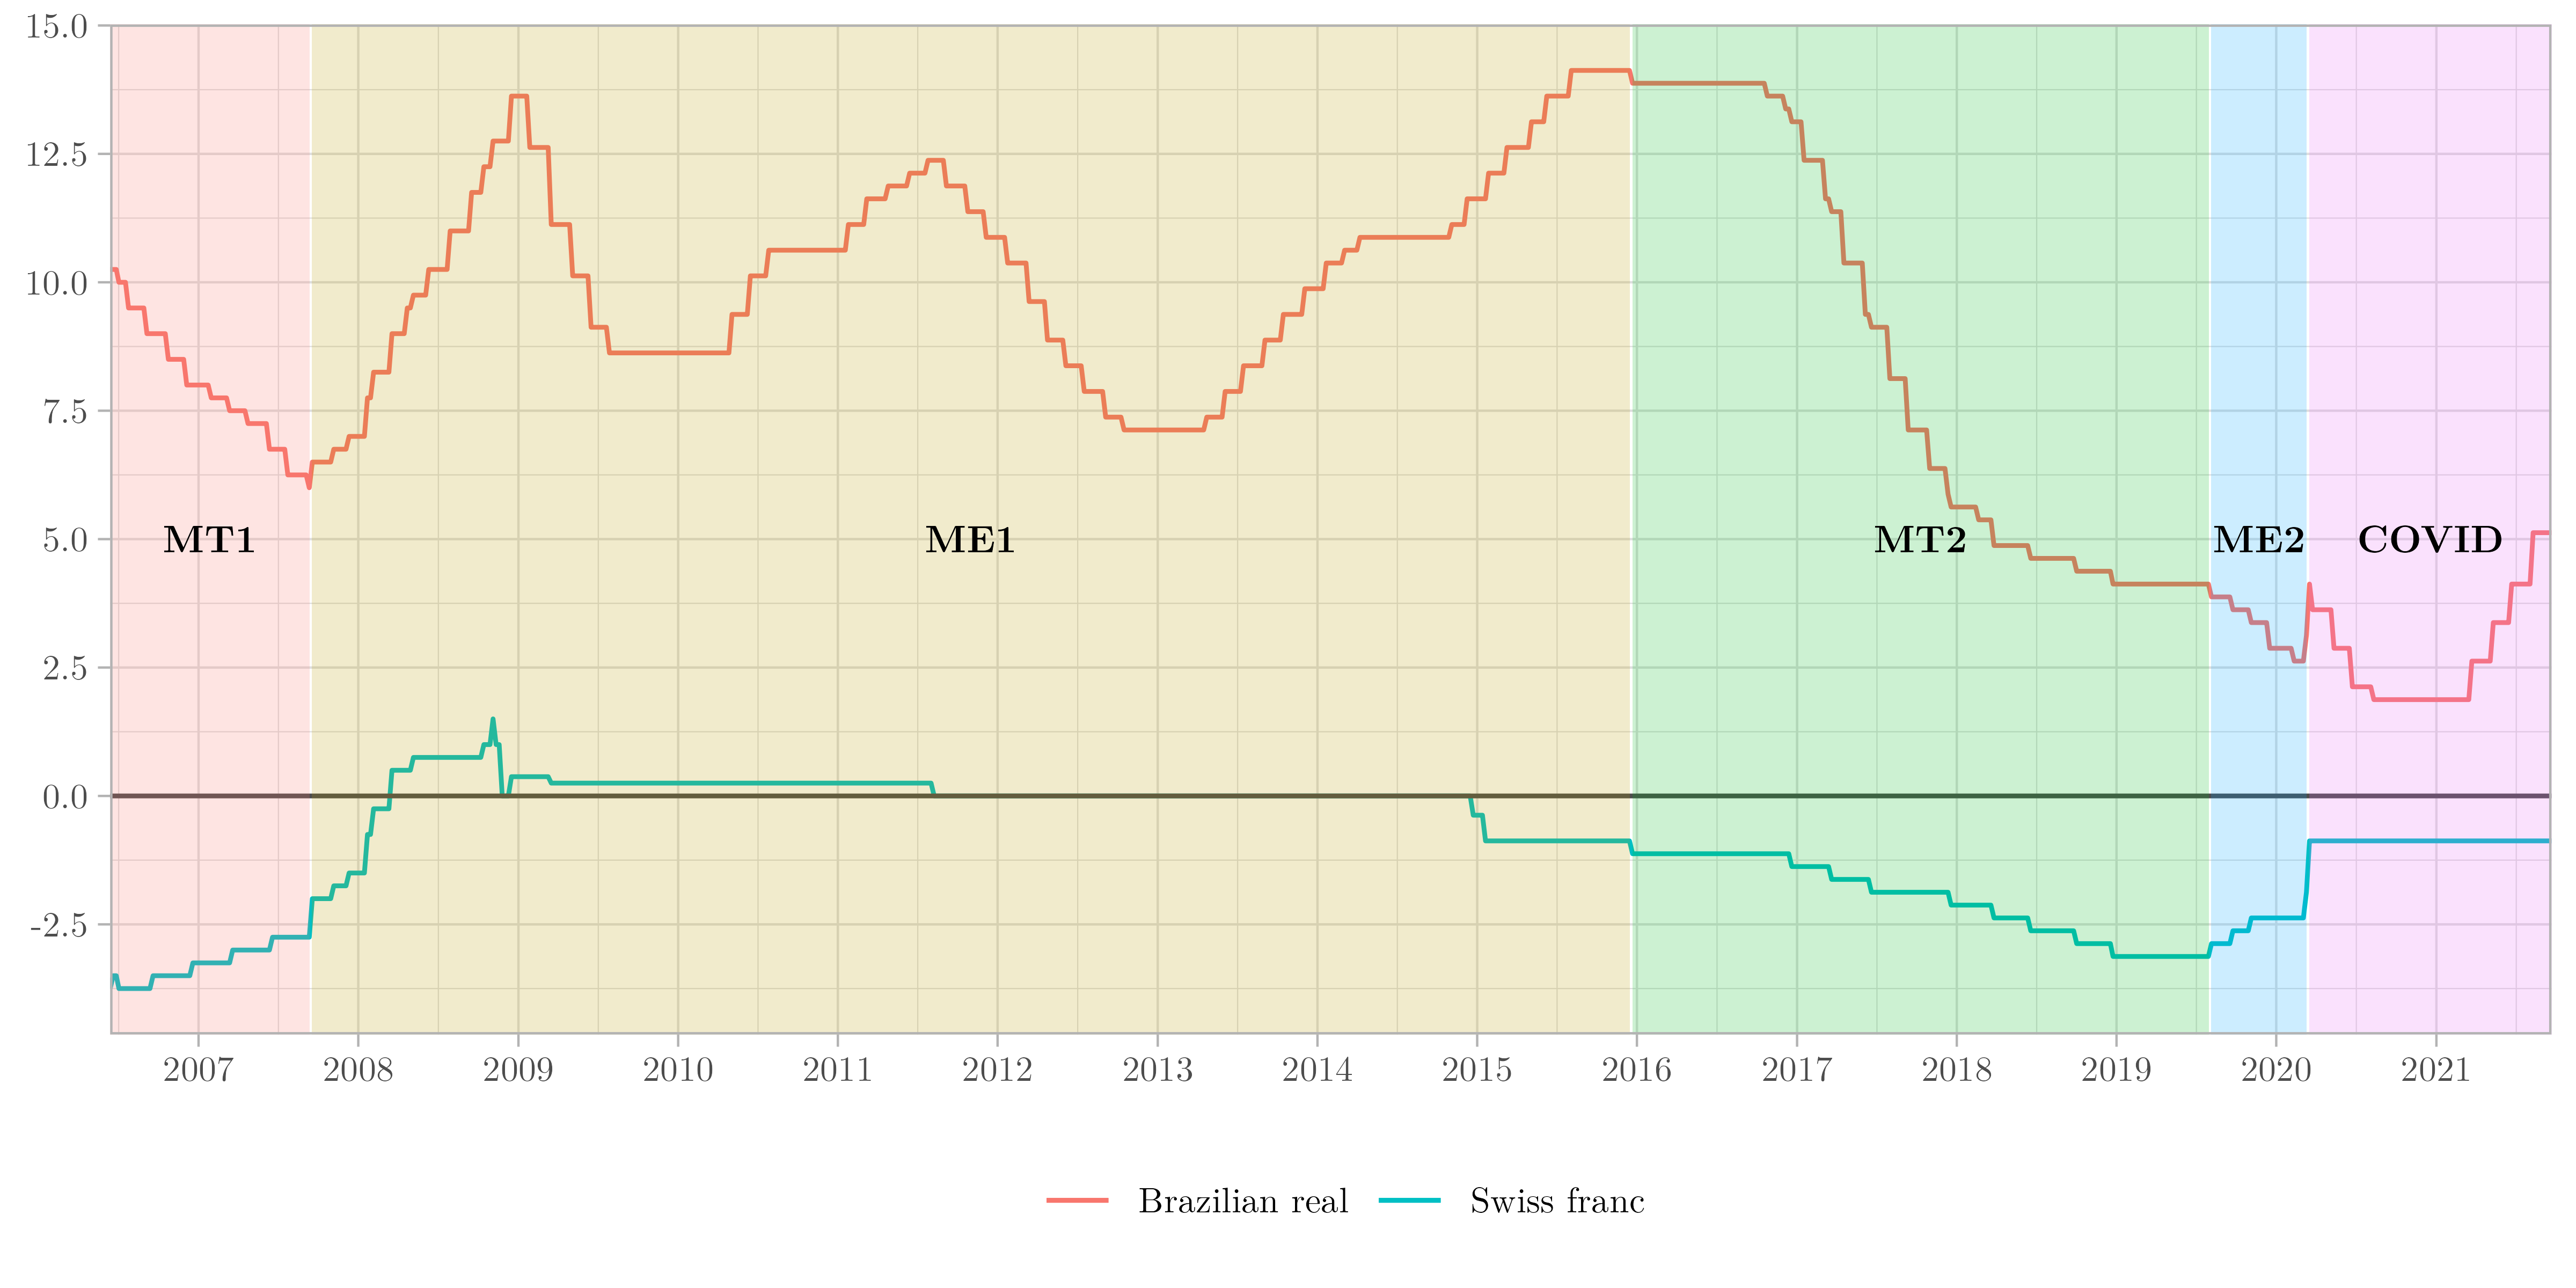
\includegraphics[width=0.99\columnwidth]{figure/CHFBRLIRD} 

}

\caption[Interest rate differentials between both Switzerland and Brazil and the United States, 2006-06-13 to 2021-09-21]{Interest rate differentials between both Switzerland and Brazil and the U.S., 2006-06-13 to 2021-09-21 \\ \scriptsize \textit{Source:} Bank for International Settlements (BIS).}\label{fig:Figure311}
\end{figure}

Figure \ref{fig:Figure312} presents the scatter plot of the pair hedge funds net (long minus short) positions (\(NP\)) and interest rate differentials (\(IRD\)) for both the Swiss franc and Brazilian real.

\begin{figure}[!ht]

{\centering 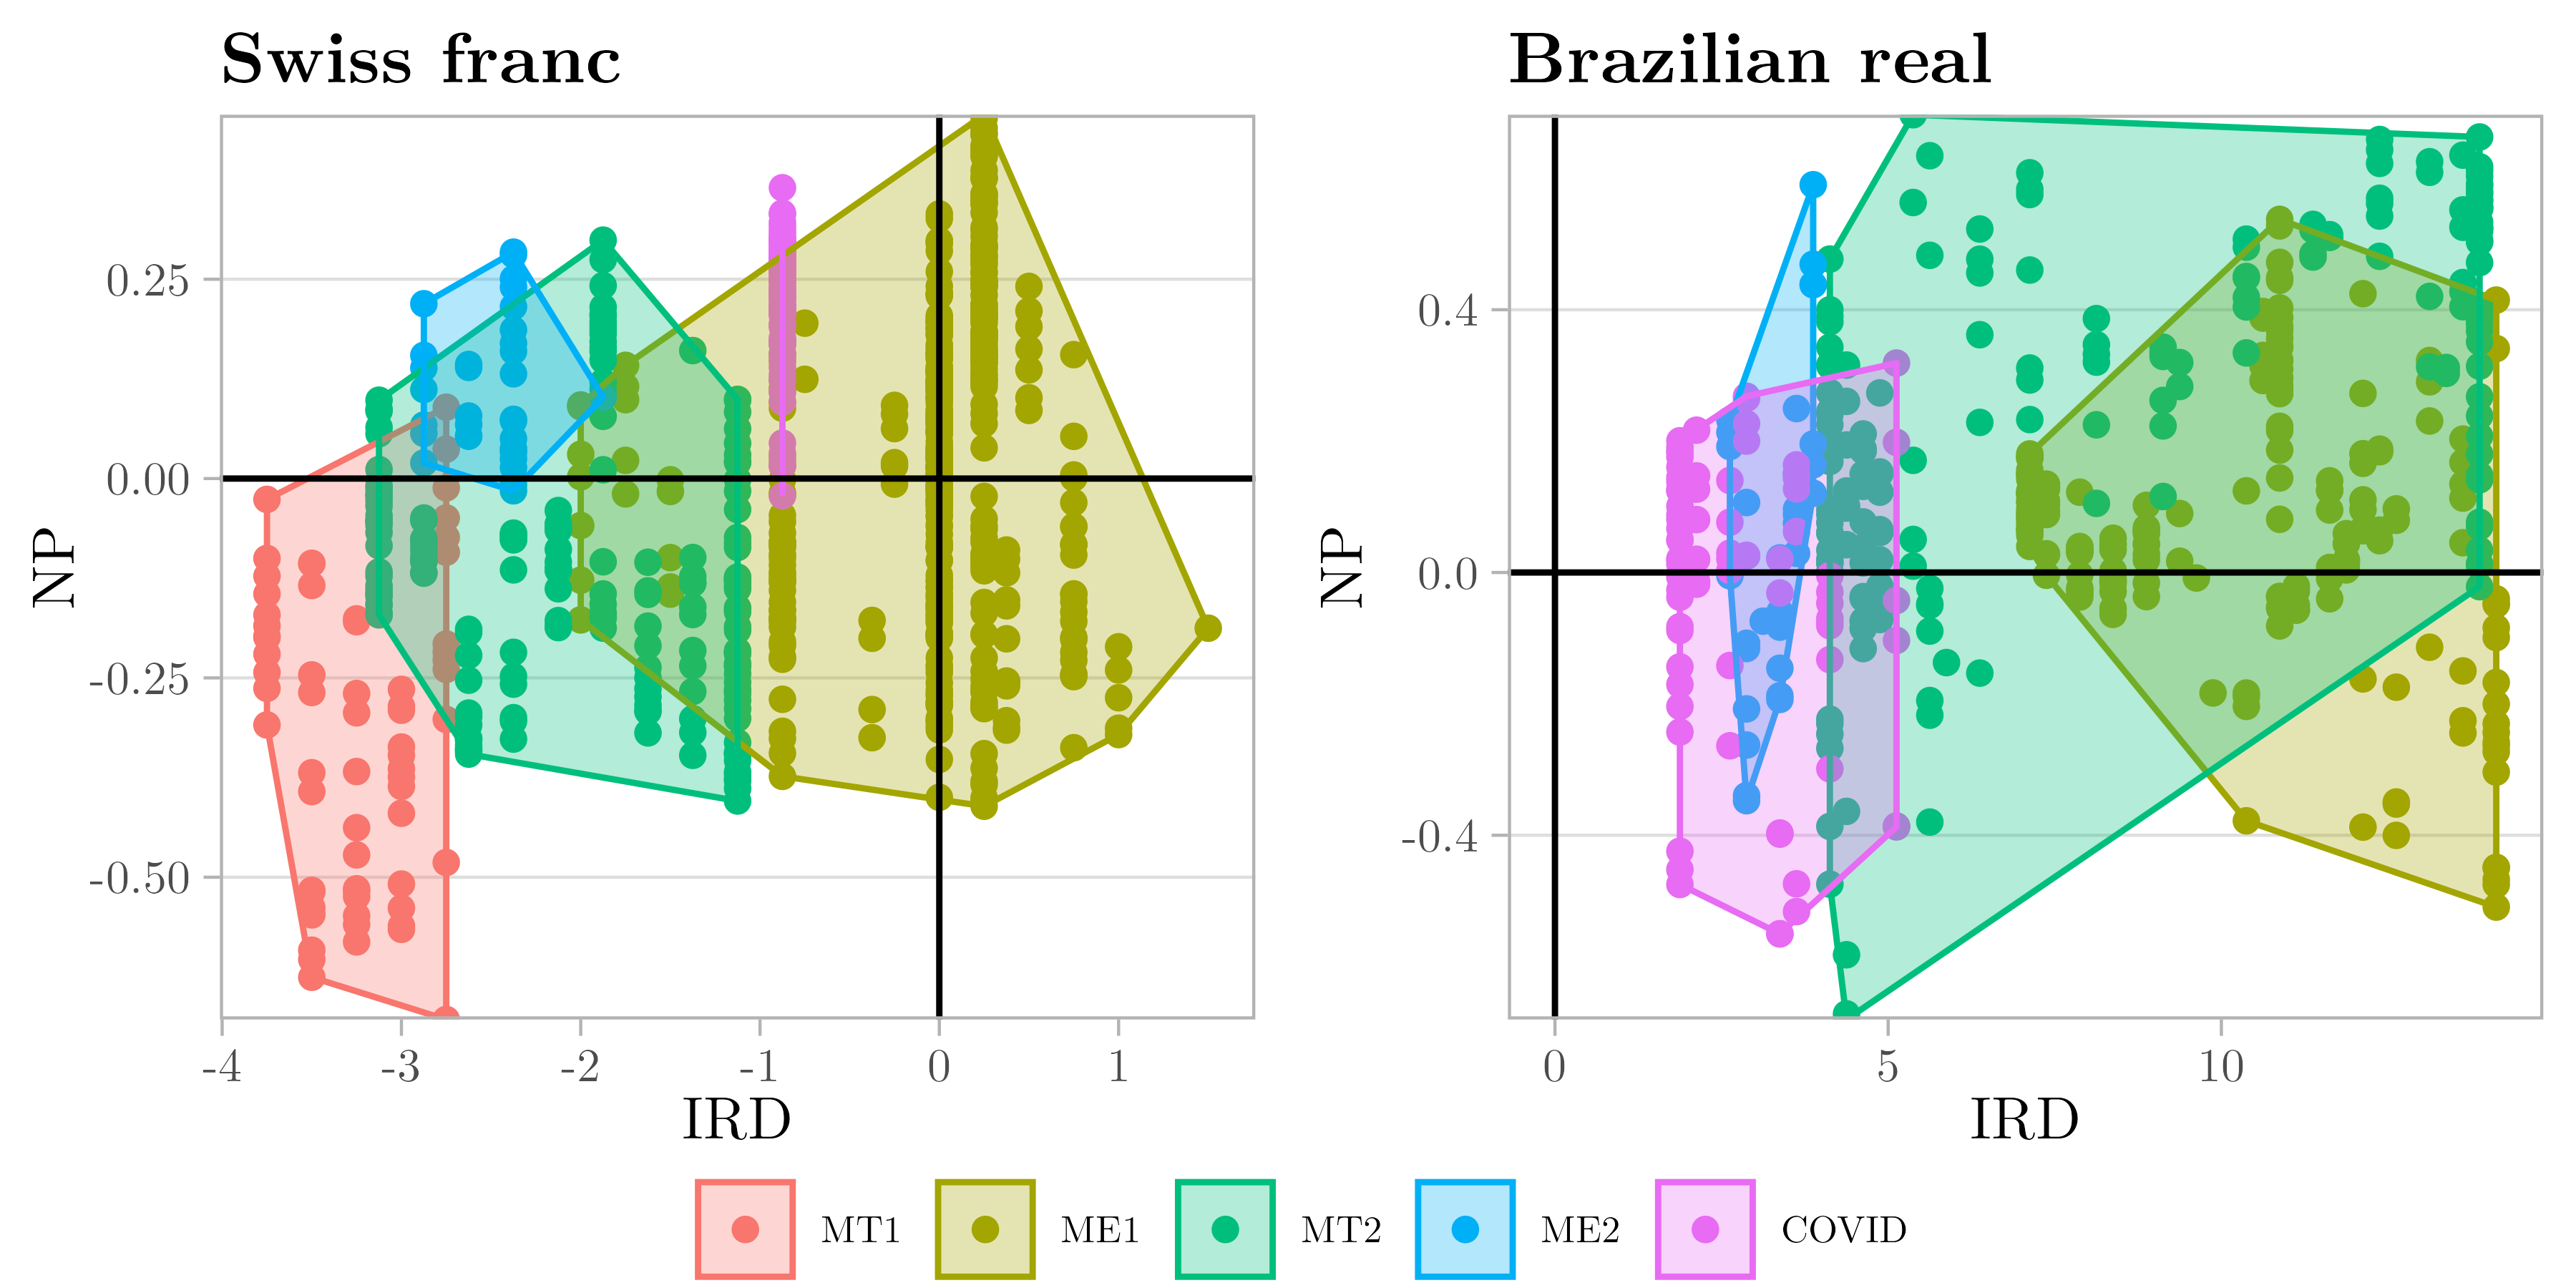
\includegraphics[width=0.99\columnwidth]{figure/CHFBRL_HF} 

}

\caption[Hedge funds net positions and interest rate differentials for the Swiss franc (2006-06-13 to 2021-09-21) and the Brazilian real (2011-04-05 to 2021-09-21)]{Hedge funds net positions and interest rate differentials for the Swiss franc (2006-06-13 to 2021-09-21) and the Brazilian real (2011-04-05 to 2021-09-21) \\ \scriptsize \textit{Source:} Commodity Futures Trading Comission (CFTC) and Bank for International Settlements (BIS).}\label{fig:Figure312}
\end{figure}

In line with \textcite[\text{p.} 43]{fong2013}, we focus on hedge funds because of their ``ability to use leverage and derivatives for speculation''. In the classical approach to measure the carry trade, the funding currency is characterized by negative values in both net positions and interest rate differentials. On the other hand, positive values for both variables identify a target currency. While the former is also called net short, the latter is commonly known as net long. As complemented by Figures \ref{fig:FigureA38} and \ref{fig:FigureA39} in Appendix \ref{appendixa5}, none of the currencies available at the CFTC data present this binary behavior. Nevertheless, for CHF and BRL, most of the observations are in line with the expected behavior.\footnote{273 observations in the funding currency quadrant (lower left-hand corner) for the CHF and 350 observations in the target currency quadrant (upper right-hand corner) for the BRL.}

More strikingly, as shown by Figure \ref{fig:Figure313}, currencies may change their role depending on the U.S. monetary policy. This is consistent with the practitioner approach developed in \textcite[Chpater 4.3, \text{pp.} 62-68]{willer2020}, where they mention the USD bull and bear markets\footnote{``Financial analysts and stock market commentators frequently classify the stock market as being a bull or a bear market, and often they define a bear market as occurring when the market declines by a (large) fixed percent, say 20\%, and a bull market as occurring when the market rises by a (large) fixed percent, again say 20\%.'' \autocite[\text{p.} 983]{jansen2010}}, which are connected to the monetary policy swings.

\begin{figure}[!ht]

{\centering 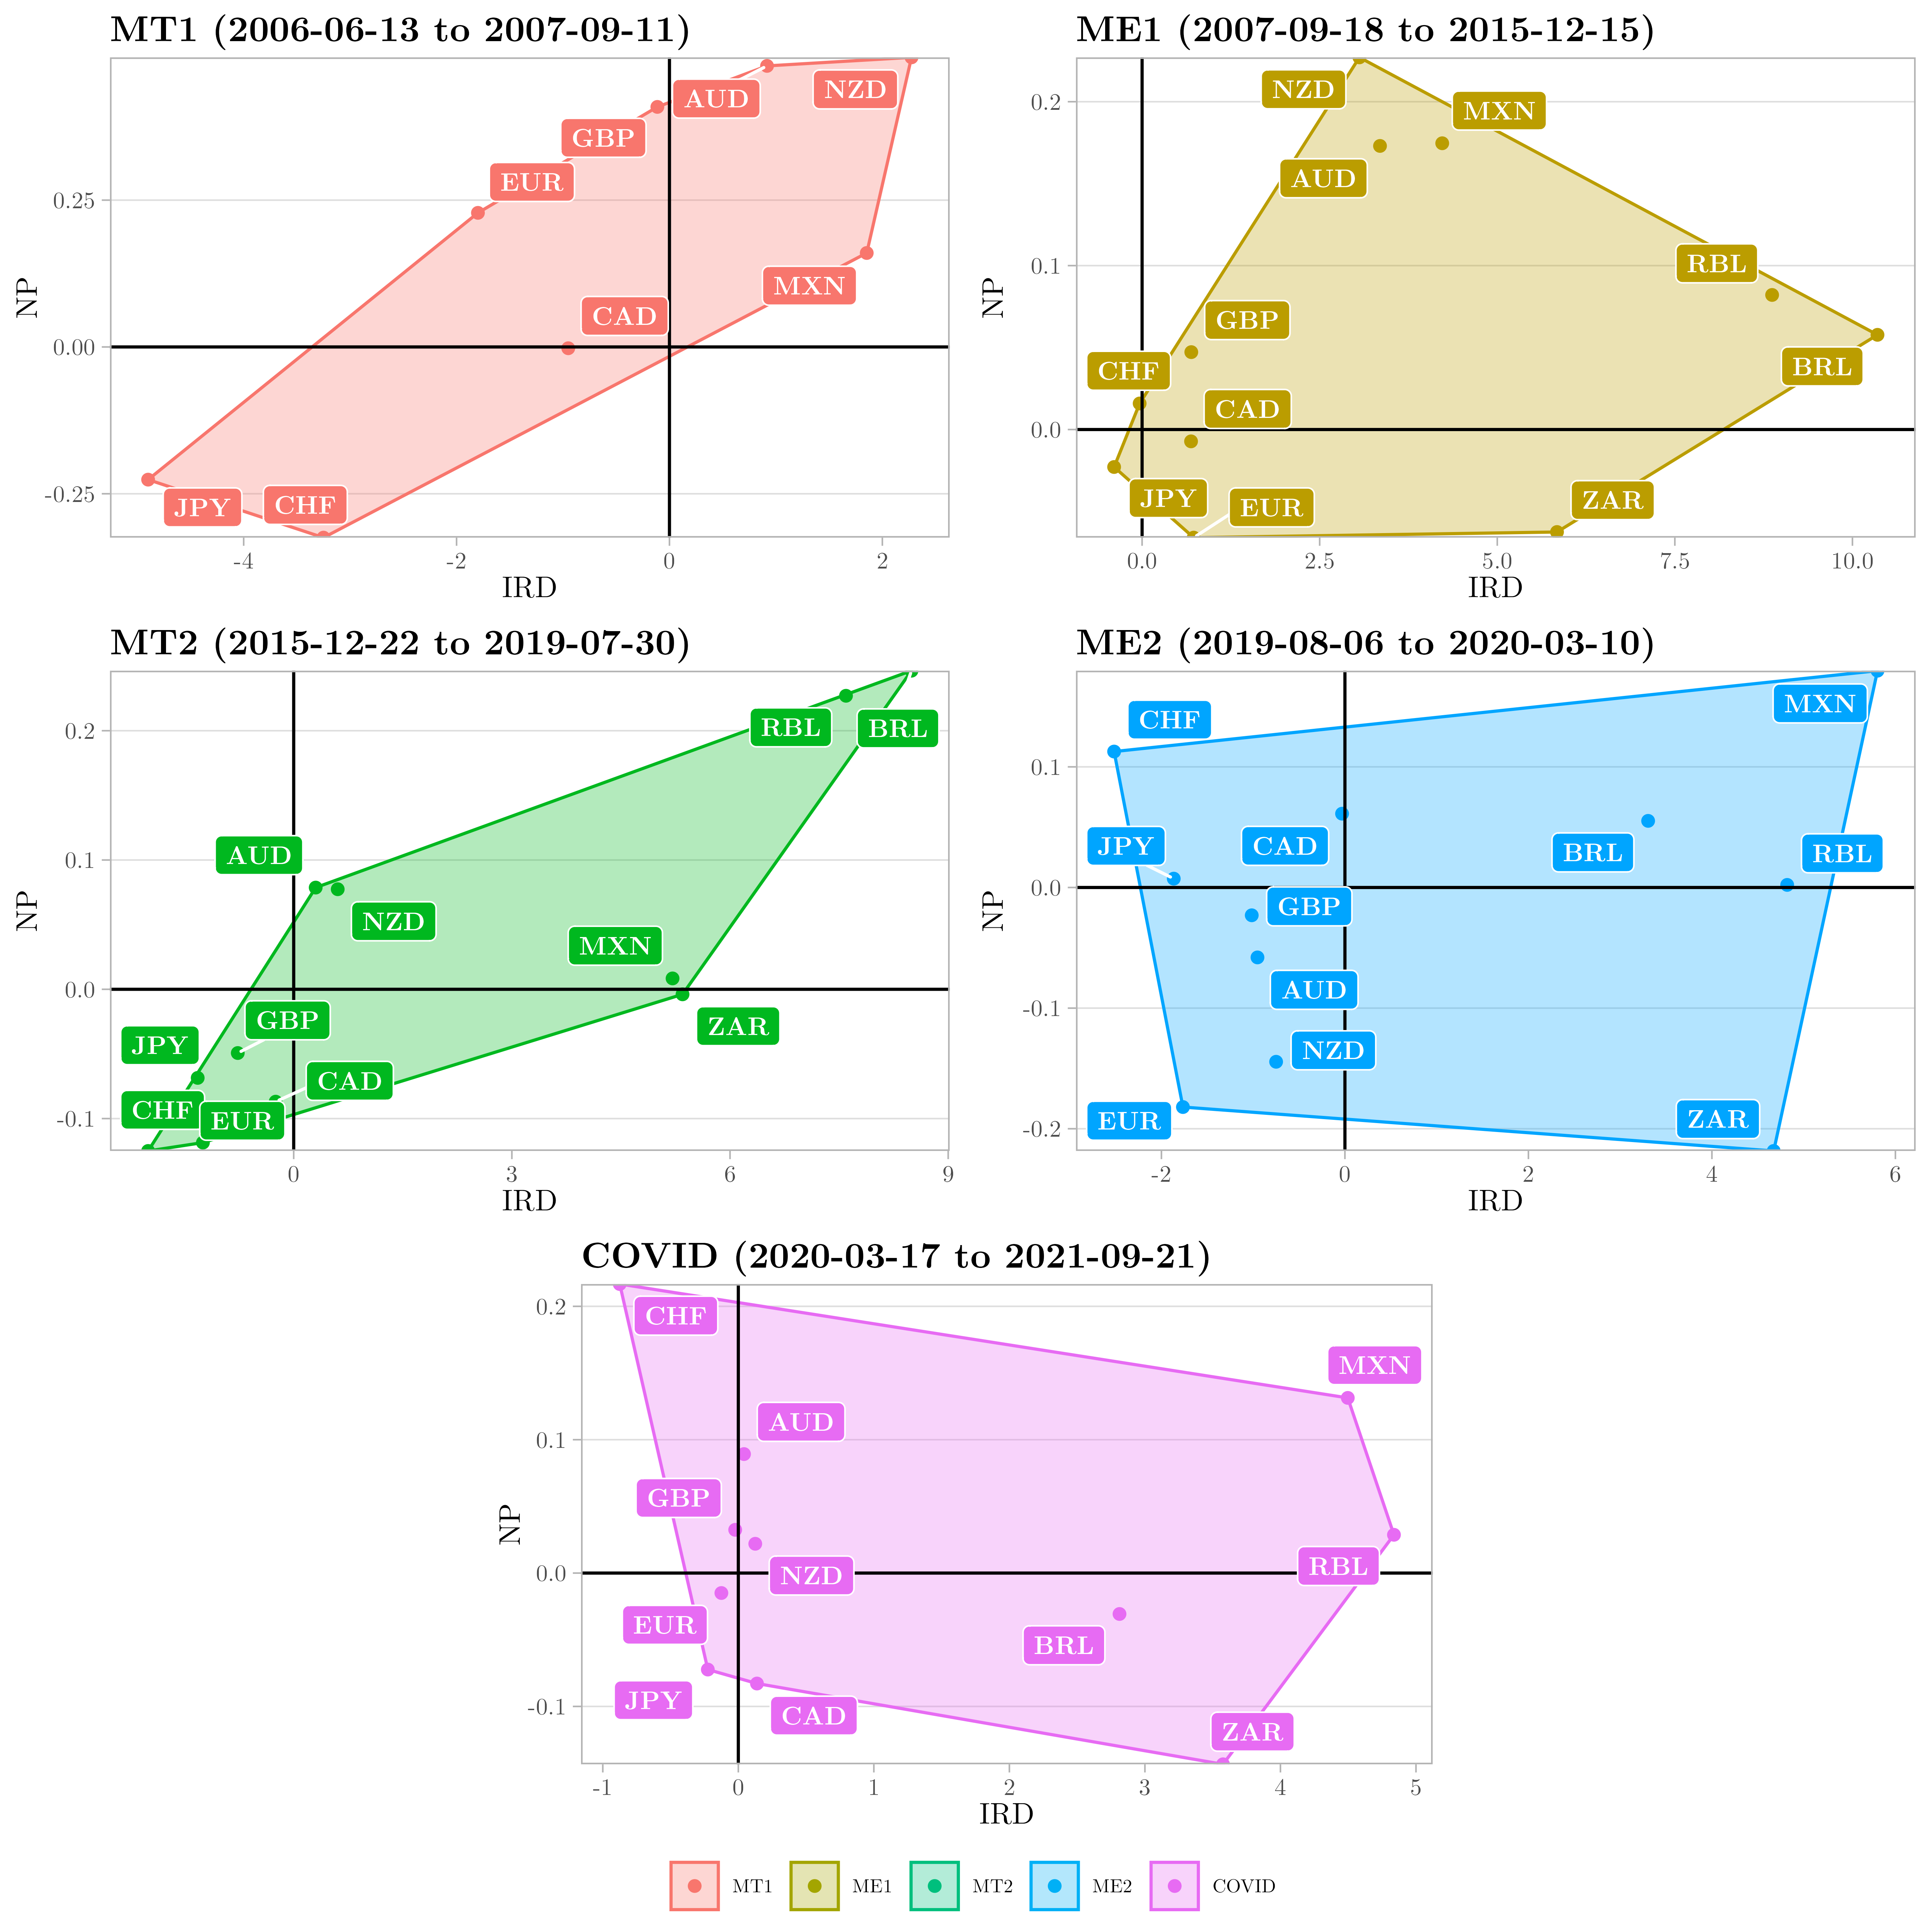
\includegraphics[width=0.99\columnwidth]{figure/TOG_HF} 

}

\caption[Hedge funds net positions and interest rate differentials for several currencies in different periods of U.S. monetary policy, mean values, 2006-06-13 to 2021-09-21]{Hedge funds net positions and interest rate differentials for several currencies in different periods of U.S. monetary policy, mean values, 2006-06-13 to 2021-09-21 \\ \scriptsize \textit{Source:} Commodity Futures Trading Comission (CFTC) and Bank for International Settlements (BIS).}\label{fig:Figure313}
\end{figure}

On average, the Swiss franc behaves as a funding currency during the periods of U.S. monetary tightening and as a safe haven currency in the periods of U.S. monetary easing. The same cannot be said to the Brazilian real, except for the COVID-19 period, in which it behaved more like a funding currency. This possible funding behavior is somewhat related to other target currencies, with which a negative interest rate differential is present, not the U.S. dollar. Nevertheless, the plausible explanation is that investors are just short positioned due to the elevated risk. In the five periods, other emerging market currencies (Mexican peso and Russian ruble) presented themselves as target currencies. The possible change in the role expressed by the Brazilian real is supported by research on the Chinese renminbi:

\begin{quote}
In addition, some emerging economies would likely have higher interest rates than China, suggesting that residents of these economies would have an incentive to use the renminbi as a funding currency rather than just as an investing currency. So although China will likely have relatively higher interest rates than advanced economies, the renminbi may not necessarily evolve as an investing currency only. \autocite[\text{p.} 320]{he2016}
\end{quote}

\hypertarget{twofour}{%
\section{The real economy got carried away}\label{twofour}}

\noindent When describing the linkages between exchange rates and financial factors, \textcite[\text{p.} 49]{claessens2018} mention that ``{[}t{]}he carry trade puzzle illustrates that the literature is still struggling to integrate a number of financial factors.'' More specifically, the carry trade literature lacks studies that document its effects on the real economy. In order to capture these impacts, models need to go beyond financial factors by exploring macrofinancial linkages. As defined by \textcite[\text{p.} 1]{claessens2018}:

\begin{quote}
Macrofinancial linkages centre on the two-way interactions between the real economy and the financial sector. Shocks arising in the real economy can be propagated through financial markets, thereby amplifying business cycles. Conversely, financial markets can be the source of shocks, which, in turn, can lead to more pronounced macroeconomic fluctuations. The global dimensions of these linkages can result in cross-border spillovers through both real and financial channels.
\end{quote}

Regarding the direction of the macrofinancial linkages, this thesis focuses on assessing the carry trade shocks on the real economy. In the current U.S. dollar-centered system, developing countries' currencies tend to suffer more from the negative international spillovers generated by financial shocks than their developed countries counterparties\footnote{Notwithstanding, there are also problems in the relation among the U.S. dollar and other central currencies. For example, ``the euro area is disproportionately more sensitive to shocks in the US macroeconomy and financial sector, resulting in an asymmetric cross-border spillover pattern between the two economies.'' \autocite[\text{p.} 5]{gerba2020}}. One key reason is the subordination of developing countries' central banks to developed countries' monetary policy. Given the interdependence of monetary policy in the actual international monetary system, developing countries' central banks must always consider developed countries' monetary policy in their actions. Contrarily, developed countries' central banks are not subject to monetary policies implemented in developing countries. Therefore, given the dependency, developing countries' central banks are not entirely free to focus solely on their own economy. Further, in addition to the analysis of the macrofinancial linkages, a political approach is needed to understand better how the asymmetrical power structure in the actual international monetary system fosters carry trade activity.

Broadly, the main research question investigated in this thesis is: \textbf{How does carry trade impact the real economy activity?} In order to pursue it, three chapters are structured. While Chapter \ref{three} (\emph{Carry trade in developing and developed countries: A Granger causality analysis with the Toda-Yamamoto approach}) explores developed and developing countries, Chapter \ref{four} (\emph{Carry trade and negative interest rate policy in Switzerland: Low-lying fog or storm?}) focuses on Switzerland. In closing, Chapter \ref{five} (\emph{The political economy of carry trade: The real economy got carried away in Switzerland and Brazil}) focuses on Switzerland and Brazil. Overall, the core methodological idea is that

\begin{quote}
``science requires both reductionism\footnote{It ``means a bottom up approach to understand complex natural phenomena by `reducing' them to their fundamental parts and studying their inter actions under controlled conditions. {[}\ldots{]} Reductionist approaches help us to break complex systems down into their components, and each piece can be studied individually by way of disciplinary and sub-disciplinary approaches. If we know the parts, the dynamics of the whole system can be derived.'' \autocite[\text{p.} 42]{thomas2021}} and holism\footnote{It ``asserts that things have certain properties as a whole, which cannot be explained based on its components parts. The word `holism' is from Greek, meaning all, whole, entire, or total.'' \autocite[\text{p.} 43]{thomas2021}}. We usually dismantle complex systems into various component parts employing reductionist approaches to get first hand information about the system. In most cases, this also allows scientists to put the pieces together again by way of holism.'' \autocite[\text{p.} 43]{thomas2021}
\end{quote}

Both Chapters \ref{three} and \ref{four} are empiric-focused, aiming to investigate carry trade's linkages to financial factors. In this reductionist approach, there are limitations to capturing the real economy: (i) it is not directly measured by any variable in the estimated models and (ii) there is a focus on a very limited group of countries/currencies. Nevertheless, two channels link both monetary and real sides of the economy, rejecting the classical dichotomy: exchange rates and financial markets.

First, the exchange rate channel is central to analyzing the carry trade effects on the real economy. \textcite{rodrik2008} uses the \emph{real} exchange rate to investigate how this channel impacts economic growth in developing countries. His results confirm that an exchange rate undervaluation positively impacts economic growth, which is also supported by \textcite{seraj2020}. Since carry trade takes place in financial markets, the use of the \emph{nominal} exchange rate is preferable. Above and beyond, central banks all around the world constantly scrutinize exchange rates. \textcite[\text{p.} 12]{gadanecz2013} highlight that

\begin{quote}
{[}a{]}s exchange rates are key prices in the economy, their level and flexibility have implications for resource allocation and growth. Countries may attempt to influence the level of exchange rates and restrict their flexibility depending on, among other factors, the choice of monetary regime and the development of the financial system. Indeed, over the past decade, many emerging economies have done this. Such choices imply real trade-offs, with both short- and long-run implications.
\end{quote}

Second, carry trade is inherently related to the financial market channel. In this sense, stock market indexes and ``investor sentiment index''/``volatility index'' \autocite{shaikh2017} are used in the estimated models in both chapters. The core theoretical point is that financial markets impact the real economy. On the one hand, this impact is understood to be positive. \textcite[\text{p.} 688]{levine1997} elaborates a literature survey of the relationship between finance and economic activity, where he concludes that ``the preponderance of theoretical reasoning and empirical evidence suggests a positive, first-order relationship between financial development and economic growth.'' Moreover, ``{[}a{]}s countries get richer over time or as one shifts from poor to richer countries, {[}\ldots{]} stock markets become larger, as measured by market capitalization relative to GDP, and more liquid, as measured by trading relative to GDP, market capitalization, and stock price variability.'' \autocite[\text{pp.} 716-717]{levine1997} \textcite{levine1998}, \textcite{arestis2001} and \textcite{beck2004} also find evidence for the positive impact of stock markets on economic growth.

On the other hand, speculation on financial markets can create market instability, negatively impacting the real economy \autocite{depaula2013}. As phrased by \textcite[\text{p.} 262]{hermann2014}, ``the actions of speculators in financial markets (necessary to provide liquidity to secondary markets) and of financial institutions in liberalized markets can have a destabilizing effect in such markets.'' More specifically, regarding Brazil and other Latin American countries, \textcite[\text{p.} 1907]{shen2006} find that ``financial liberalization mitigate the positive impacts of stock market development on growth.'' Moreover, \textcite{moosa2018} finds a negative relation between financialization, measured in terms of the ratio of publicly traded shares to GDP, and economic growth. Notably, ``{[}i{]}n low-income countries, even a small transfer of resources from real economic activity to stock trading exerts a significant adverse impact on growth in countries that do not have much resources.'' \autocite[3412]{moosa2018} Additionally, the investor sentiment index VIX\footnote{``The VIX Index is a calculation designed to produce a measure of constant, 30-day expected volatility of the U.S. stock market, derived from real-time, mid-quote prices of S\&P 500® Index (SPX℠) call and put options. On a global basis, it is one of the most recognized measures of volatility -- widely reported by financial media and closely followed by a variety of market participants as a daily market indicator.'' \autocite{cboeexchange2021}} helps capture the pervasive effects of carry trade on the real economy by connecting this speculative activity with systemic risk.

By using holism as a method, Chapter \ref{five} is built upon the insights obtained from Chapters \ref{three} and \ref{four}. Most importantly, a global economy model is estimated to capture the carry trade effects on the real economy. The proposed empirical framework is a Bayesian global vector autoregressive model (BGVAR)\footnote{This is possible thanks to the \texttt{R} package \texttt{BGVAR} developed by \textcite{bock2021}. More information about this package is supplied by \textcite{bock2020}.}, which follows the pioneering work by \textcite{pesaran2004}. In this broader model, the main research question is pursued by directly analyzing the relationship between carry trade and real economy variables (e.g., gross domestic product). The aim is to model world economy dynamics in the search for the carry trade linkages. In this context, the international monetary spillovers are essential to understanding better the carry trade behavior. Regarding the literature on these spillovers, \textcite{miranda-agrippino2021}, \textcite{cavaca2021}, \textcite{bernoth2021} and \textcite{breitenlechner2021} offer key insights.

As stressed by \textcite{hauzenberger2021} and \textcite{jorda2021}, low (and even negative) interest rates will remain present for an extended period in the world economy. This type of monetary policy fosters the carry trade activity. While developed countries, like Switzerland, implement these policies to address their own economic problems, there are important monetary spillovers on developing countries, like Brazil. In our asymmetric-structured international monetary system, financialization amplifies the negative monetary spillovers generated by the fostered carry trade activity. Centrally, the biggest problem with the carry trade is not its short-run impacts, but rather its long-lasting long-run effects.

Carry trade is an unproductive activity linked, to a large extent, to rentiers' behavior. To maximize the efficiency of their profit-seeking speculative activity, a continuous ``sabotage in the financial system'' \autocite{nesvetailova2020} occurs. Against this background, carry trade not only crowds out the productive activity and enhances financial instability but also contributes to aggravating income inequalities. Inextricably linked to, both financialization of commodities \autocite{basak2016,caldentey2020} and ``subordinated financial integration'' \autocite{kaltenbrunner2018a} also contribute to the uneven development of developing countries. Essentially, in the context of the carry trade, income distribution in favor of rentiers is a consequence of monetary policy.\footnote{Research exploring the distributional impacts of monetary policy is vast, as shown by this non-exhaustive list: \textcite{moore1990}; Smithin \autocite*{smithin1996,smithin2020}; \textcite{thorbecke2001}; Rochon and Setterfield \autocite*{rochon2007,rochon2008,rochon2012}; \textcite{seccareccia2016}; \textcite{seccareccia2017}; \textcite{davtyan2017}; \textcite{guerello2018}; \textcite{casiraghi2018}; \textcite{rochon2021}; \textcite{holm2021}; \textcite{bonifacio2021}; \textcite{amberg2021}; \textcite{ybrayev2021}. Particularly, see \textcite{kappes2021} for a recent survey of the empirical literature.} As a result, central banks need to review their role in order to tame these negative spillovers. Otherwise, the real economy will continue to get carried away by the carry trade.

\begin{savequote}
We must recognise, I think, that there can be a real divergence of
interest; and we must not expect of central banks a degree of
international disinterestedness far in advance of national sentiment and
of the behaviour of the other organs of national government.
\qauthor{--- \textcite[\text{p.} 257]{keynes1978}}\end{savequote}



\hypertarget{three}{%
\chapter[Carry trade in developing and developed countries: A Granger causality analysis with the Toda-Yamamoto approach]{\texorpdfstring{Carry trade in developing and developed countries: A Granger causality analysis with the Toda-Yamamoto approach\footnote{This chapter is a slightly modified version of my article published in the journal Economics Bulletin \autocite[see][]{tomio2020}.}}{Carry trade in developing and developed countries: A Granger causality analysis with the Toda-Yamamoto approach}}\label{three}}

\minitoc 

\hypertarget{threeone}{%
\section{Introduction}\label{threeone}}

\noindent Due to the increased interconnectedness of global financial markets at the end of the 20\textsuperscript{th} century and the beginning of the 21\textsuperscript{st} century, interest rate differentials among countries have fostered speculative capital flows seeking higher yields. Central bankers worldwide set their base interest rate accordingly with their mission. Every country has its singularity and characteristics, which demands a unique set of monetary policies. In this sense, some countries are obliged to set high interest rates (usually developing and underdeveloped countries), while others present low interest rates (notably, developed countries). Speculators profit from this type of structure to seek financial gains, contradicting what is expected by the uncovered interest rate parity (UIP), one of the fundamental theories of international finance.

Currency speculation is not a new phenomenon, showing its first institutional developments in the Middle Ages \autocite{accominotti2016}. Foreign exchange markets (Forex or FX) have augmented their size significantly in recent decades. The financialization of the world economy has led the daily turnover in Forex markets to surpass 40 times the daily amount of world trade of goods in U.S. dollars in 2019, as shown in Figure \ref{fig:Figure31}. In 1989, the ratio FX to trade was 21, highlighting the strengthening of financialization in Forex markets during the last two decades.

\begin{figure}[ht]

{\centering 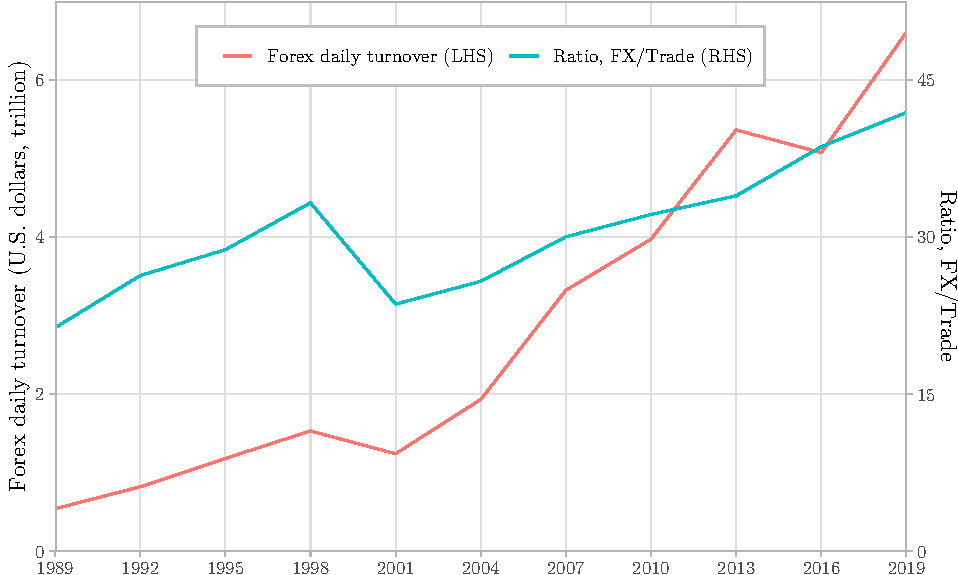
\includegraphics[width=0.99\columnwidth]{_main_files/figure-latex/Figure31-1} 

}

\caption[Forex daily turnover and ratio between Forex daily turnover and daily trade (ratio FX/Trade), 1989-2019]{Forex daily turnover and ratio between Forex daily turnover and daily trade (ratio FX/Trade), 1989-2019 \\ \scriptsize \textit{Source:} Bank for International Settlements (BIS) for the Forex daily turnover. International Monetary Fund (IMF) for trade, using the sum of exports and imports of goods in current U.S. dollars, divided by 20 (business days). Both series are daily means for April.}\label{fig:Figure31}
\end{figure}

One of the leading financial operations in the Forex market is the currency carry trade. By targeting ``international interest differentials'', carry traders (investors applying the carry trade investment strategy) ``shift their asset holdings from low interest-rate currencies to higher-return currencies'' \autocite[\text{p.} 3]{grenville2010}.

With the speculators' positioning data supplied by the U.S. Commodity Futures Trading Commission (CFTC) Large Trader Reporting Data, I explore the relationship of the carry trade and its related financial variables. The carry trade literature can be divided into two big strands. On the one hand, there is a vast literature exploring carry trade returns with the use of portfolio optimization \autocites[e.g.,][]{clarida2009,cenedese2014,doskov2015,kang2020}. On the other hand, there is another strand criticizing carry trade and its consequences \autocites[e.g.,][]{miranda-agrippino2013,goda2019}. Nonetheless, as shown by \textcite{disyatat2013}, this strand of literature lacks robust empirical analyses.

In this sense, this paper fills a gap in the carry trade literature by trying to approach both strands. \textcite{chuffart2020} also make use of CFTC data to investigate the effects of carry trade. This is a paper that is close to the main idea explored here: carry trade (proxied by real positioning) impacts other financial variables. Meanwhile, their focus is to assess the impacts of carry trade on the real economy during the Quantitative Easing period in Japan.

My results show evidence of the relationship between carry trade and four related financial variables (interest rate differentials, market sentiment, local stock indexes, and the U.S. stock index) in ten currencies (Australian dollar, Brazilian Real, Canadian dollar, Euro, British Pound, Japanese Yen, Mexican Peso, New Zealand dollar, Russian Ruble, and Swiss Franc). With two different periods based on the U.S. monetary policy (monetary easing and tightening), the Granger causality tests with the \textcite{toda1995} technique show relevant differences and similarities in the long-term relationship of these variables for each analyzed country.

\hypertarget{threetwo}{%
\section{Methodology and Data}\label{threetwo}}

By following the model estimated by \textcite{nishigaki2007}, this article focuses on the relationship among carry trade (\(CT\)), nominal exchange rates (\(ER\)), interest rates differentials (\(IRD\)), market sentiment (\(VIX\)), local stock market indices (\(SM\)), and the U.S. stock market index (\(SMUS\)).

\hypertarget{threetwoone}{%
\subsection{Methodology}\label{threetwoone}}

The applied model follows the VAR system as it is similarly proposed by \textcite{amiri2012}.\footnote{See the VAR model equations in the Appendix \ref{appendixb1}.}

The null hypothesis of the Granger causality test is that the dependent variable does not Granger cause the independent variable (excluded variable). To find evidence that the other variables Granger cause \(CT\), conditions in Table \ref{tab:Table31} must hold, as it is shown in Equation \eqref{eq:b2}\textsuperscript{2}. Table \ref{tab:Table32} shows the conditions for the Granger causality in the direction of other variables to \(CT\), following Equations \eqref{eq:b1}, \eqref{eq:b3}, \eqref{eq:b4}, \eqref{eq:b5}, and \eqref{eq:b6}\textsuperscript{2}.

\begin{table}[H]

\caption{\label{tab:Table31}Conditions for the Granger causality from the other variables to $CT$}
\centering
\fontsize{10}{12}\selectfont
\begin{tabular}[t]{>{}llllll}
\toprule
Direction & $ER$$\rightarrow$$CT$ & $IRD$$\rightarrow$$CT$ & $VIX$$\rightarrow$$CT$ & $SM$$\rightarrow$$CT$ & $SMUS$$\rightarrow$$CT$\\
\midrule
\textbf{Condition} & $\alpha_{21i}\neq0\forall_i$ & $\gamma_{21i}\neq0\forall_i$ & $\delta_{21i}\neq0\forall_i$ & $\psi_{21i}\neq0\forall_i$ & $\phi_{21i}\neq0\forall_i$\\
\bottomrule
\end{tabular}
\end{table}

\begin{table}[H]

\caption{\label{tab:Table32}Conditions for the Granger causality from $CT$ to the other variables}
\centering
\fontsize{10}{12}\selectfont
\begin{tabular}[t]{>{}llllll}
\toprule
Direction & $CT$$\rightarrow$$ER$ & $CT$$\rightarrow$$IRD$ & $CT$$\rightarrow$$VIX$ & $CT$$\rightarrow$$SM$ & $CT$$\rightarrow$$SMUS$\\
\midrule
\textbf{Condition} & $\beta_{11i}\neq0\forall_i$ & $\beta_{31i}\neq0\forall_i$ & $\beta_{41i}\neq0\forall_i$ & $\beta_{51i}\neq0\forall_i$ & $\beta_{61i}\neq0\forall_i$\\
\bottomrule
\end{tabular}
\end{table}

It is worth highlighting that the ordering of the variables does not change the results from the Granger causality tests.

\hypertarget{threetwotwo}{%
\subsection{Data}\label{threetwotwo}}

As a proxy for carry trade (\(CT\)), the weekly data provided by the U.S. Commodity Futures Trading Commission's (CFTC) Commitments of Traders Report (COTR) is used. This report only provides information for 12 currencies. Excluding the Euro FX/British Pound and the South African Rand, my dataset is composed of ten of them (Australian dollar - AUD, Brazilian Real - BRL, Canadian dollar - CAD, Euro - EUR, British Pound - GBP, Japanese Yen - JPY, Mexican Peso - MXN, New Zealand dollar - NZD, Russian Ruble - RBL, and Swiss Franc - CHF). The reasons for exclusion are that the former is not a pair with the U.S. dollar, and the latter lacks data.

There are some caveats in the use of this proxy. Usually, exchanges in currency markets are over-the-counter (OTC) operations, complicating the modeling of carry trade activity \autocite{galati2007,gubler2014}. Not only CFTC data represent a small fraction of carry trade, but some traders may also be using these contracts for other purposes \autocite{curcuru2011}. Each contract has information that is not publicly available, leaving space for misinterpretation. Nonetheless, as pointed out by \textcite{bankforinternationalsettlements2015}, CFTC data is a reliable indicator of trends in carry trade activity. Also, it is the best publicly available data on speculative traders.

Using the number of contracts of non-commercial traders, I calculate the carry trade as the ratio of positions, as proposed by \textcite{nishigaki2007}. For target currencies, the ratio is calculated by dividing long positions by short positions (\(CT\)). Conversely, short positions over long positions are the ratio for funding currencies (\(CTF\)). As pointed out by \textcite[\text{, p.} 438]{curcuru2011}, ``engagement in carry trades could be indicated by a net short futures position in the funding currency, paired with a net long futures position in the target currency.'' Therefore, using a specific ratio for each type of currency (target or funding) is more adequate to model its behavior.

The interest rate differential gives the classification of target and funding currencies. If the difference between the country's policy interest rate and the U.S. policy interest rate (\(IRD\)) is positive, the country's currency is classified as a target currency. Contrariwise, a negative value for \(IRD\) indicates a funding currency. In this case, following \textcite{gubler2014}, the interest rate differential (\(IRDF\)) is given by the difference between the U.S. policy interest rate and the country's policy interest rate. Figure \ref{fig:Figure32} illustrates the results for the \(IRD\).

\begin{figure}

{\centering 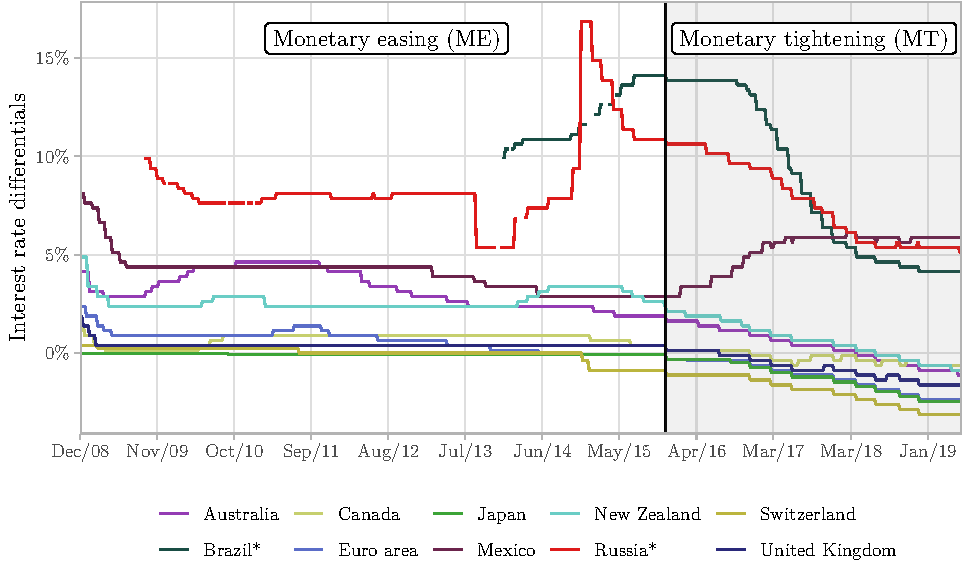
\includegraphics[width=0.99\columnwidth]{_main_files/figure-latex/Figure32-1} 

}

\caption[Difference between the country’s policy interest rate and the U.S. policy interest rate, in per cent]{Difference between the country’s policy interest rate and the U.S. policy interest rate, in per cent \\ \scriptsize *Gaps are present due to lack of data in other variables.}\label{fig:Figure32}
\end{figure}

As shown in Figure \ref{fig:Figure32}, currencies changed their classification according to the U.S. monetary policy movements. During the monetary easing (ME) period, only the currencies of Japan and Switzerland are classified as funding currencies, being the U.S. dollar the target currency. During the monetary tightening (MT) period, there are significant changes. First, the currencies of Canada, the Euro area, and the United Kingdom reclassify as funding currencies. Second, the currencies of Australia and New Zealand present target and funding classifications, creating respectively two subsamples MTT and MTF. Table \ref{tab:Table33} shows the number of observations for each country and sample.

\begin{table}

\caption{\label{tab:Table33}Sample description}
\centering
\fontsize{10}{12}\selectfont
\begin{tabular}[t]{lccccc}
\toprule
\multicolumn{2}{c}{\textbf{ }} & \multicolumn{4}{c}{\textbf{Sample}} \\
\cmidrule(l{3pt}r{3pt}){3-6}
\textbf{Country} & \textbf{Period} & \textbf{ME} & \textbf{MT} & \textbf{MTT} & \textbf{MTF}\\
\midrule
Australia & 12/30/2008 - 06/25/2019 & 364 &  & 118 & 66\\
Brazil* & 01/14/2014 - 06/25/2019 & 94 & 184 &  & \\
Canada & 12/30/2008 - 06/25/2019 & 364 & 184 &  & \\
Euro area & 12/30/2008 - 06/25/2019 & 364 & 184 &  & \\
Japan & 12/30/2008 - 06/25/2019 & 364 & 184 &  & \\
Mexico & 12/30/2008 - 06/25/2019 & 364 & 184 &  & \\
New Zealand & 12/30/2008 - 06/25/2019 & 364 &  & 130 & 54\\
Russia* & 10/06/2009 - 06/25/2019 & 315 & 184 &  & \\
Switzerland & 12/30/2008 - 06/25/2019 & 364 & 184 &  & \\
United Kingdom & 12/30/2008 - 06/25/2019 & 364 & 184 &  & \\
\bottomrule
\multicolumn{6}{l}{\rule{0pt}{1em}\textit{\footnotesize{*}} \footnotesize{Period differs from other countries due to lack of data.}}\\
\end{tabular}
\end{table}

Additionally, an exogenous dummy variable for the tapering period (TAPER) in the monetary easing (ME) period is included. TAPER starts in May 2013, with Ben Bernanke mentioning for the first time the possibility of tapering \autocite{chari2017}. It ends with the first hike in the U.S. policy interest rate on December 15 2015. This dummy is critical to account for the period wherein the quantitative easing monetary policies started to unwind.

Table \ref{tab:Table34} shows the detailed description of each variable\footnote{Descriptive statistics is supplied in Appendix \ref{appendixb2}.}. Based on \textcite{donnelly2019}, nominal exchange rates (\(ER\)) are in the same form as used by market practitioners. Market sentiment is given by (\(VIX\)). To account for the stock market activity of each country and in the U.S., main market indexes are used (\(SM\) and \(SMUS\), respectively). Overall, I follow the same group of variables proposed by \textcite{nishigaki2007}.




\begin{table}[ht]

\caption{\label{tab:Table34}Description of variables}
\centering
\resizebox{\linewidth}{!}{
\begin{threeparttable}
\begin{tabular}[t]{c>{\raggedright\arraybackslash}p{11,5cm}c}
\toprule
\textbf{Variable} & \textbf{Definition} & \textbf{Source}\\
\midrule
\multirow{3}{*}[0pt]{$ER$} & Nominal exchange rates (AUDUSD, USDBRL, USDCAD, EURUSD, USDJPY, USDMXN, NZDUSD, USDRBL, USDCHF, and GBPUSD) & \multirow{3}{*}[0pt]{BIS}\\
\addlinespace

$CT$ & Ratio of long positions over short positions (Long/Short) & CFTC\\
\addlinespace

$CTF$ & Ratio of short positions over long positions (Short/Long) & CFTC\\
\addlinespace

\multirow{2}{*}[0pt]{$IRD$} & Difference between the country’s policy interest rate and the U.S. policy interest rate & \multirow{2}{*}[0pt]{BIS}\\
\addlinespace

\multirow{2}{*}[0pt]{$IRDF$} & Difference between the U.S. policy interest rate and the country’s policy interest rate & \multirow{2}{*}[0pt]{BIS}\\
\addlinespace

\multirow{5}{*}[0pt]{$VIX$} & (1) CBOE DJIA Volatility Index (Australia, Canada, Japan, Mexico, New Zealand, Russia, Switzerland, and the United Kingdom)\newline  (2) CBOE Brazil ETF Volatility Index (Brazil)\newline  (3) CBOE EuroCurrency ETF Volatility Index (Euro area) & \multirow{5}{*}[0pt]{FRED}\\
\addlinespace

\multirow{10}{*}[0pt]{$SM$} & (1) S$\&$P/ASX 200, $\textasciicircum$AXJO (Australia)\newline (2) IBOVESPA, $\textasciicircum$BVSP (Brazil)\newline (3) S$\&$P/TSX, $\textasciicircum$GSPTSE (Canada)\newline (4) EURONEXT 100, $\textasciicircum$N100 (Euro area)\newline (5) NIKKEI 225, $\textasciicircum$N225 (Japan)\newline (6) S$\&$P/BMV IPC, $\textasciicircum$MXX (Mexico)\newline (7) S$\&$P/NZX 50, $\textasciicircum$NZ50 (New Zealand)\newline (8) MOEX Russia, IMOEX.ME (Russia)\newline (9) Swiss Market Index, $\textasciicircum$SSMI (Switzerland)\newline (10) FTSE 100, $\textasciicircum$FTSE (United Kingdom) & \multirow{10}{*}[0pt]{Yahoo Finance*}\\
\addlinespace

$SMUS$ & S$\&$P 500, $\textasciicircum$GSPC (United States) & Yahoo Finance*\\
\bottomrule
\end{tabular}
\begin{tablenotes}[para]
\item \textit{\footnotesize{*}} 
\item \footnotesize{Data is gathered using the R package {quantmod} (function GetSymbols), developed by \textcite{fong2013}. The R package {BatchGetSymbols}, written by \textcite{ryan2020}, was used to confirm that the data collected was clean. Due to problems with data for Russia, data from the Moscow Exchange (MOEX) was used for cleaning.}
\end{tablenotes}
\end{threeparttable}}
\end{table}

\hypertarget{threethree}{%
\section[Estimation results]{\texorpdfstring{Estimation results\footnote{A replication pack with the commands (Stata 13 Do-file) and data is available \href{http://www.accessecon.com/includes/CountdownloadPDF.aspx?Type=Other_data\&ID=EB-19-00720}{here}. Appendix \ref{appendixb} provide the supplemental material.}}{Estimation results}}\label{threethree}}

\hypertarget{threethreeone}{%
\subsection{Preliminary procedures}\label{threethreeone}}

In order to capture long-term impacts, I opt to use all variables in levels. The \textcite{toda1995} technique is applied to deal with non-stationary variables.

As pointed out by \textcite{amiri2012}, the \textcite{toda1995} approach is useful to circumvent models' misspecification with non-stationary variables. In order to guarantee the usual asymptotic chi-square null distribution of the Wald tests, lagged exogenous variables are added to each non-stationary variable. The number of lags depends on the integration order (\(d\)) and the maximum lag length of the VAR model (\(p\)). Hence, the number of lags of these variables in the final models is specified by \(d\) plus \(p\), generating a modified Wald test (MWald test). Therefore, ``it is clearly desirable to have a testing procedure which is robust to the integration and cointegration properties of the process so as to avoid the possible pretest biases.'' \autocite[\text{p.} 226]{toda1995}

First, to find the integration order (\(d\)), I apply the unit-roots test with one structural break with unknown breakpoints developed by \textcite{clemente1998}. In the AO (Additive Outlier) model, equation \eqref{eq:21} is estimated to remove the deterministic part of the variable:

\begin{equation}
y_t = \mu + d_1DU_{1t} + \widetilde{y}_t
\label{eq:21}
\end{equation}

In the next step, the test searches for the minimal \(t\)-ratio for the unit-root hypothesis (\(\rho=1\)) in the following model

\begin{equation}
\widetilde{y}_t = \sum_{i=0}^k\omega_{1t}DTB_{1t-1} + \rho\widetilde{y}_{t-1}\sum_{i=0}^kc_i\Delta\widetilde{y}_{t-1} + e_t
\end{equation}

Table \ref{tab:Table35} summarizes the results of the unit-roots tests, with details in Appendix \ref{appendixb3}.

\begin{table}[ht]

\caption{\label{tab:Table35}Stationary variables, I(0)}
\centering
\fontsize{10}{12}\selectfont
\begin{tabular}[t]{lcccc}
\toprule
\textbf{Country} & \textbf{ME} & \textbf{MT} & \textbf{MTT} & \textbf{MTF}\\
\midrule
Australia & $CT$, $VIX$ &  & $VIX$, $SM$ & $ER$, $VIX$\\
Brazil & $VIX$, $SMUS$ & * &  & \\
Canada & $CT$, $VIX$ & * &  & \\
Euro area & $IRD$, $VIX$ & $CTF$, $VIX$, SM &  & \\
Japan & $VIX$ & $ER$, $SM$ &  & \\
Mexico & $ER$, $IRD$, $VIX$ & $ER$, $IRD$ &  & \\
New Zealand & $VIX$ &  & $ER$, $VIX$ & *\\
Russia & $VIX$, $SM$ & * &  & \\
Switzerland & $CTF$, $ER$, $VIX$ & $ER$, $SM$ &  & \\
United Kingdom & $CT$, $IRD$, $VIX$ & $SM$ &  & \\
\bottomrule
\multicolumn{5}{l}{\rule{0pt}{1em}\textit{\footnotesize{*}} \footnotesize{All variables are I(1).}}\\
\end{tabular}
\end{table}

Second, tests for the optimal lag length are applied to choose the maximum lag length of the VAR model (\(p\)). These tests generate two statistics (likelihood-ratio - LR and Akaike's final prediction error - FPE) and three information criteria (Akaike - AIC, Hannan and Quinn - HQIC, and Schwarz's Bayesian - SBIC). I do not rely solely on these tests\footnote{See detailed results in the Appendix \ref{appendixb4}.} to choose \(p\) because residual autocorrelation may be present. Thus, Lagrange-multiplier (LM) tests for residual autocorrelation are also computed. With \(d\) and \(p\), the final robustness check is the stability test, i.e., eigenvalue stability condition\footnote{Check Appendix \ref{appendixb5} for further details.}.

\hypertarget{threethreetwo}{%
\subsection[Empirical results]{\texorpdfstring{Empirical results\footnote{Individual (country) stability tests, model structures and extended results are provided in Appendix \ref{appendixb6}, Appendix \ref{appendixb7} and Appendix \ref{appendixb8}, respectively.}}{Empirical results}}\label{threethreetwo}}

Table \ref{tab:Table36} shows the results for the target currencies during the ME period. On the one hand, all variables are jointly Granger causing carry trade (\(CT\)) in Australia, Brazil, the Euro area, Mexico, and the United Kingdom. Individually, the exchange rate (\(ER\)) is a good predictor for the carry trade in almost all countries (except for Canada, Mexico, and Russia). Additionally, other variables preceding carry trade are interest rate differentials (\(IRD\)) for the Euro area, market sentiment (\(VIX\)) for Australia, and the local stock market index (\(SM\)) for Brazil.

\begin{table}[H]

\caption{\label{tab:Table36}Granger causality tests for target currencies, ME period}
\centering
\resizebox{\linewidth}{!}{
\begin{tabular}[t]{lccccccccccc}
\toprule
\multicolumn{1}{c}{ } & \multicolumn{6}{c}{Variable Granger causes $CT$} & \multicolumn{5}{c}{$CT$ Granger causes variable} \\
\cmidrule(l{3pt}r{3pt}){2-7} \cmidrule(l{3pt}r{3pt}){8-12}
  & $ER$$\rightarrow$$CT$ & $IRD$$\rightarrow$$CT$ & $VIX$$\rightarrow$$CT$ & $SM$$\rightarrow$$CT$ & $SMUS$$\rightarrow$$CT$ & All$\rightarrow$$CT$ & $CT$$\rightarrow$$ER$ & $CT$$\rightarrow$$IRD$ & $CT$$\rightarrow$$VIX$ & $CT$$\rightarrow$$SM$ & $CT$$\rightarrow$$SMUS$\\
\midrule
Australia & 0.0690* & 0.3713 & 0.0440** & 0.9281 & 0.7600 & 0.0237** & 0.0107** & 0.0177** & 0.0579* & 0.0032*** & 0.3430\\
Brazil & 0.0138** & 0.8548 & 0.3617 & 0.0072*** & 0.8281 & 0.0136** & 0.7520 & 0.3516 & 0.0003*** & 0.8471 & 0.3479\\
Canada & 0.3964 & 0.9922 & 0.7171 & 0.7768 & 0.7653 & 0.6446 & 0.6495 & 0.1778 & 0.0668* & 0.4429 & 0.9260\\
Euro area & 0.0018*** & 0.0648* & 0.9997 & 0.7238 & 0.5735 & 0.0193** & 0.4133 & 0.4627 & 0.9528 & 0.8781 & 0.9076\\
Mexico & 0.4464 & 0.1380 & 0.0284 & 0.9543 & 0.7690 & 0.0841* & 0.8426 & 0.8025 & 0.6783 & 0.7541 & 0.0986*\\
New Zealand & 0.0075*** & 0.8657 & 0.4763 & 0.6224 & 0.6691 & 0.1286 & 0.2216 & 0.9520 & 0.0002*** & 0.8175 & 0.5921\\
Russia & 0.8960 & 0.9999 & 0.2621 & 0.8321 & 0.8158 & 0.9648 & 0.6354 & 0.9972 & 0.0131*** & 0.5677 & 0.8950\\
United Kingdom & 0.0001*** & 0.4233 & 0.7454 & 0.1410 & 0.5969 & 0.0008*** & 0.3816 & 0.3306 & 0.0000*** & 0.3244 & 0.8850\\
\bottomrule
\multicolumn{12}{l}{\rule{0pt}{1em}\textit{Notes: } ‘***’, ‘**’, and ‘*’ denote significance at 1\%, 5\%, and 10\% respectively. }\\
\end{tabular}}
\end{table}

On the other hand, there are statistically significant results showing that carry trade also Granger causes the other variables. Mainly, \(CT\) is anticipating movements in market sentiment for almost all countries (excluding the Euro area and Mexico), highlighting the important link with market instability. As other variables are concerned, \(CT\) precedes \(ER\), \(IRD\), and \(SM\) for Australia. The results for the Australian dollar show that carry trade impacts go further from the financial market, impacting the real economy. For Mexico, \(CT\) predicts movements in the U.S. stock market, showing evidence of their financial market linkages.

As for funding currencies during the ME period, Table \ref{tab:Table37} illustrates the results. All variables jointly Granger cause carry trade (\(CTF\)) for Japan, showing significant individual results for \(ER\) and \(VIX\). For Switzerland, \(ER\) is Granger causing \(CTF\). Moreover, there is evidence for bi-directional Granger causality between ERF and \(CTF\) for Japan. As for the Swiss case, \(CTF\) is preceding movements in the interest rate differential (\(IRDF\)). Last but not least, \(CTF\) is a good predictor of local stock prices for both Japan and Switzerland. As highlighted by \textcite{nishigaki2007}, speculative investors use funding currencies as leverage to buy other assets. With the upsurge (reduction) in short positions in the futures market, an appreciation (depreciation) in the funding currencies is expected. Therefore, a higher (lower) value of the local currency compared to the U.S. dollar may increase (decrease) investors' interest in local stock markets.

\begin{table}[H]

\caption{\label{tab:Table37}Granger causality tests for funding currencies, ME period}
\centering
\resizebox{\linewidth}{!}{
\begin{tabular}[t]{lccccccccccc}
\toprule
\multicolumn{1}{c}{ } & \multicolumn{6}{c}{Variable Granger causes $CTF$} & \multicolumn{5}{c}{$CTF$ Granger causes variable} \\
\cmidrule(l{3pt}r{3pt}){2-7} \cmidrule(l{3pt}r{3pt}){8-12}
  & $ER$$\rightarrow$$CTF$ & $IRDF$$\rightarrow$$CTF$ & $VIX$$\rightarrow$$CTF$ & $SM$$\rightarrow$$CTF$ & $SMUS$$\rightarrow$$CTF$ & All$\rightarrow$$CTF$ & $CTF$$\rightarrow$$ER$ & $CTF$$\rightarrow$$IRDF$ & $CTF$$\rightarrow$$VIX$ & $CTF$$\rightarrow$$SM$ & $CTF$$\rightarrow$$SMUS$\\
\midrule
Japan & 0.0001*** & 0.9882 & 0.0538* & 0.7254 & 0.8043 & 0.0031*** & 0.0219** & 0.7318 & 0.8856 & 0.0009*** & 0.5406\\
Switzerland & 0.0315** & 0.2420 & 0.7194 & 0.1945 & 0.3151 & 0.1662 & 0.2932 & 0.0559* & 0.0022*** & 0.0002*** & 0.4742\\
\bottomrule
\multicolumn{12}{l}{\rule{0pt}{1em}\textit{Notes: } ‘***’, ‘**’, and ‘*’ denote significance at 1\%, 5\%, and 10\% respectively. }\\
\end{tabular}}
\end{table}

Results for target currencies during the monetary tightening period are in Table \ref{tab:Table38}. Jointly, all variables Granger cause \(CT\) for Australia and Russia. For Australia, Brazil, and Mexico, \(ER\) and \(IRD\) are preceding changes in \(CT\). Also, \(VIX\) and \(SM\) Granger cause \(CT\) for Russia and Australia, respectively. Linkages to the impact of the carry trade in the real economy are supported by the Granger causality of \(CT\) to \(VIX\) and \(SM\), as shown by the results of Australia, Mexico, and New Zealand. Additionally, \(CT\) precedes changes in \(IRD\) for Australia and Brazil.

\begin{table}[H]

\caption{\label{tab:Table38}Granger causality tests for target currencies, MT period}
\centering
\resizebox{\linewidth}{!}{
\begin{tabular}[t]{lccccccccccc}
\toprule
\multicolumn{1}{c}{ } & \multicolumn{6}{c}{Variable Granger causes $CT$} & \multicolumn{5}{c}{$CT$ Granger causes variable} \\
\cmidrule(l{3pt}r{3pt}){2-7} \cmidrule(l{3pt}r{3pt}){8-12}
  & $ER$$\rightarrow$$CT$ & $IRD$$\rightarrow$$CT$ & $VIX$$\rightarrow$$CT$ & $SM$$\rightarrow$$CT$ & $SMUS$$\rightarrow$$CT$ & All$\rightarrow$$CT$ & $CT$$\rightarrow$$ER$ & $CT$$\rightarrow$$IRD$ & $CT$$\rightarrow$$VIX$ & $CT$$\rightarrow$$SM$ & $CT$$\rightarrow$$SMUS$\\
\midrule
Australia* & 0.0036*** & 0.0783* & 0.5150 & 0.5115 & 0.0144** & 0.0133** & 0.1550 & 0.0080*** & 0.0016*** & 0.0850* & 0.2292\\
Brazil & 0.0938* & 0.0429** & 0.7410 & 0.4735 & 0.6990 & 0.2299 & 0.4449 & 0.0340** & 0.7168 & 0.1873 & 0.6518\\
Mexico & 0.0075*** & 0.0142** & 0.4638 & 0.8785 & 0.6085 & 0.1219 & 0.5304 & 0.3040 & 0.0023*** & 0.0545* & 0.3163\\
New Zealand* & 0.4363 & 0.7138 & 0.1302 & 0.6977 & 0.1170 & 0.1943 & 0.2292 & 0.4252 & 0.0001*** & 0.0351** & 0.5152\\
Russia & 0.5043 & 0.2712 & 0.0001*** & 0.4899 & 0.2214 & 0.0002*** & 0.4339 & 0.6712 & 0.6069 & 0.2167 & 0.8777\\
\bottomrule
\multicolumn{12}{l}{\rule{0pt}{1em}\textit{Notes: } For Australia and New Zealand, MTT period. ‘***’, ‘**’, and ‘*’ denote significance at 1\%, 5\%, and 10\% respectively. }\\
\end{tabular}}
\end{table}

For funding currencies, Table \ref{tab:Table39} shows the results for the MT period. Except for Canada and the Euro area, all variables jointly predict \(CTF\). \(ER\) precedes \(CT\) for all countries (except for Canada). As \textcite{gubler2014} pointed out for the Swiss Franc as a funding currency, nominal exchange rate fluctuations are a good predictor of carry trade with the U.S. dollar as a target currency. For Switzerland, both \(IRDF\) and \(SMUS\) Granger cause \(CTF\). With the \(IRDF\) peaking at this period for the Swiss economy, carry trade provides excellent opportunities to borrow in Swiss francs and invest with leverage in the U.S. stock market. As pointed out by \textcite{vallet2016}, Switzerland has an advantage of ``interest rates bonus''. For the Euro area, \(IRDF\) is Granger causing \(CTF\). As for the local stock markets, their movement precedes the carry trade activity. As shown by \textcite{nishigaki2007}, with the possibility to use leverage with carry trade, international speculative investors can borrow (in the funding currency) and invest locally (domestic stock market).

\begin{table}[H]

\caption{\label{tab:Table39}Granger causality tests for funding currencies, MT period}
\centering
\resizebox{\linewidth}{!}{
\begin{tabular}[t]{lccccccccccc}
\toprule
\multicolumn{1}{c}{ } & \multicolumn{6}{c}{Variable Granger causes $CTF$} & \multicolumn{5}{c}{$CTF$ Granger causes variable} \\
\cmidrule(l{3pt}r{3pt}){2-7} \cmidrule(l{3pt}r{3pt}){8-12}
  & $ER$$\rightarrow$$CTF$ & $IRDF$$\rightarrow$$CTF$ & $VIX$$\rightarrow$$CTF$ & $SM$$\rightarrow$$CTF$ & $SMUS$$\rightarrow$$CTF$ & All$\rightarrow$$CTF$ & $CTF$$\rightarrow$$ER$ & $CTF$$\rightarrow$$IRDF$ & $CTF$$\rightarrow$$VIX$ & $CTF$$\rightarrow$$SM$ & $CTF$$\rightarrow$$SMUS$\\
\midrule
Australia* & 0.0323** & 0.1012 & 0.8550 & 0.0715* & 0.1909 & 0.0656* & 0.1040 & 0.3168 & 0.7488 & 0.9954 & 0.4580\\
Canada & 0.6226 & 0.6228 & 0.4557 & 0.7414 & 0.1372 & 0.3900 & 0.0185** & 0.4607 & 0.0000*** & 0.0747** & 0.0289**\\
Euro area & 0.0759* & 0.0279** & 0.7845 & 0.3672 & 0.6791 & 0.1033 & 0.0994* & 0.4433 & 0.0342** & 0.7538 & 0.9454\\
Japan & 0.0412** & 0.5194 & 0.3446 & 0.0001*** & 0.1677 & 0.0000*** & 0.8205 & 0.3287 & 0.6732 & 0.0451** & 0.1237\\
New Zealand* & 0.0134** & 0.1053 & 0.8448 & 0.2399 & 0.7215 & 0.0718* & 0.2880 & 0.2086 & 0.0242** & 0.7772 & 0.7968\\
Switzerland & 0.0295** & 0.0913* & 0.1613 & 0.3978 & 0.0066*** & 0.0052*** & 0.6266 & 0.1635 & 0.3141 & 0.0136** & 0.1481\\
United Kingdom & 0.0008*** & 0.9577 & 0.3457 & 0.5971 & 0.8893 & 0.0411** & 0.0972* & 0.5902 & 0.9149 & 0.2962 & 0.0423**\\
\bottomrule
\multicolumn{12}{l}{\rule{0pt}{1em}\textit{Notes: } For Australia and New Zealand, MTF period. ‘***’, ‘**’, and ‘*’ denote significance at 1\%, 5\%, and 10\% respectively. }\\
\end{tabular}}
\end{table}

Additionally, as Table \ref{tab:Table39} shows, \(CTF\) predicts \(ER\) for Canada, the Euro area, and the United Kingdom. As far the market sentiment is concerned, \(CTF\) Granger causes it for Canada, the Euro area and New Zealand. In terms of stock markets, there is significant evidence of Granger causality from carry trade to (1) \(SM\) for Canada, Japan, and Switzerland; (2) \(SMUS\) for Canada and the United Kingdom.

Although using different datasets and methodologies, my results are similar to \textcite{klitgaard2004}, \textcite{mogford2006}, \textcite{nishigaki2007}, \textcite{gubler2014} and \textcite{mulligan2018}.

\hypertarget{threefour}{%
\section{Conclusions}\label{threefour}}

This paper fills a gap in the carry trade literature with the use of CFTC data to empirically explore target and funding currencies during the periods of monetary easing and tightening in the U.S.. The empirical approach with the Granger causality tests with the \textcite{toda1995} technique is also a novelty in this literature. Instead of focusing on the short-term, these new empirical results take into consideration long-term effects to better understand the dynamics of the carry trade in the selected countries.

By focusing on the U.S. futures market, which is one of the largest in the world, my results show evidence of different behavior of carry traders along with different currencies and U.S. monetary policies. During the monetary easing period, the group of target currencies is much bigger than in the monetary tightening period.

Overall, for both target and funding currencies and both periods, the exchange rate is a good predictor of carry trade. Similarly, when the related financial variables (interest rate differentials, market sentiment, and local and U.S. stock indexes) are jointly considered, there is evidence that they precede movements in the carry trade activity. The Granger causality from carry trade to market sentiment points to another similarity, highlighting the linkage between speculative investments and market instability.

For target currencies, the bi-directional Granger causality of interest rates differentials and carry trade clarifies the importance of the latter for monetary policy. Central banks from Brazil and Mexico deliberately use the interest rate policy to administrate the exchange rate, impacting speculative foreign capital movements (including carry trade).

Finally, during the monetary tightening period, both \(CT\) and \(CTF\) Granger cause stock market indexes. For target currencies, there is reasonable evidence that carry trade is preceding the movements of the stock markets of Australia, Mexico, and New Zealand. As far funding currencies are concerned, carry trade predicts fluctuations in the stock market indexes of Canada, Japan, and Switzerland. One of the main differences from target to funding currencies in this period is that the carry trade Granger causes the U.S. stock market, as shown by the results of Canada and the United Kingdom. Additionally, carry trade is Granger causing market sentiment in this period, which indicates a possible linkage of these speculative operations to systemic risk.

\begin{savequote}
Treasury therefore assesses, based on a range of evidence and
circumstances, that at least part of Switzerland's exchange rate
management over the four quarters through June 2020, and particularly
its foreign exchange intervention, was for purposes of preventing
effective balance of payments adjustments. Hence, Treasury has
determined under the 1988 Act that Switzerland is a currency
manipulator.
\qauthor{--- U.S. Department of the Treasury \autocite*[\text{p.} 5]{unitedstatesdepartmentofthetreasury2020}}\end{savequote}



\hypertarget{four}{%
\chapter[Carry trade and negative interest rate policy in Switzerland: Low-lying fog or storm?]{\texorpdfstring{Carry trade and negative interest rate policy in Switzerland: Low-lying fog or storm?\footnote{This chapter is a joint-work with Guillaume Vallet. Submitted to a journal; currently under review.}}{Carry trade and negative interest rate policy in Switzerland: Low-lying fog or storm?}}\label{four}}

\minitoc 

\hypertarget{fourone}{%
\section{Introduction}\label{fourone}}

\noindent The COVID-19 crisis has mobilized central banks to an extent rarely seen in history, even during crises. Similar to the 2008 ``Great recession'' crisis, far-sweeping measures were enforced to avert the risk of financial turmoil and restore confidence in the global economy. Indeed, the 2020 crisis has increased global uncertainty on financial markets as well as countries' economic vulnerability, which is likely to negatively affect the economies, compelling central banks to implement ``loose'' monetary policies durably. Symmetrically, such monetary policies exert consequences on monetary and financial activities. In particular, the rise in the monetary base and central banks' low or even negative interest rates policies are likely to increase global financial instability: against this backdrop, speculators can look for high returns, akin to taking high risks.

This is the case for currency carry trade activities, which can be fostered through the search for safety and liquidity in the context of international capital mobility. Specifically, with carry trade activities, central banks whose currency is perceived as ``safe haven assets'' face an increased demand, leading to exchange rate instability. The case of the Swiss franc exemplifies this: despite of very low -- and even negative sometimes -- yields, assets denominated in this currency systematically face a strong demand in case of international turmoil \autocite{guillaumin2012,vallet2016}. As a result, the Swiss franc appreciates toward other currencies. Depending on the magnitude of the appreciation, the latter puts strain on the Swiss monetary policy \autocite{gubler2014}.

In the context of the Swiss National Bank's (SNB) negative policy interest rate, this paper aims to investigate the behavior of the Swiss franc (CHF) carry trade with four target currencies (U.S. dollar, euro, Japanese yen, and British pound) by disentangling the funding currency and safe haven effects. Whereas most of the literature on the currency carry trade focuses on the estimated excess returns of currency carry portfolios, we opt to proxy the carry trade using weekly positioning data released by the U.S. Commodity Futures Trading Commission (CFTC). Our carry trade proxy is constructed with the volume of hedge funds (leveraged funds) contracts, following \textcite{fong2013}. More specifically, we refer to the Swiss franc carry trade as the strategy of shorting the Swiss franc (funding currency) to build long positions in the target currencies\footnote{On currency futures, a short (long) position is an obligation to sell (buy) currencies at an agreed rate and a specified future date.}.

The main contribution of this paper to the existing literature is the novel approach to investigate thoroughly the implied Swiss franc carry trade by exploring: (i) the hedge funds' behavior with CFTC data, i.e., quantity data \autocite{dupuy2021}, not prices as proxied by the expected excess returns, (ii) the period of negative policy interest rates and (iii) the dual role of the Swiss franc as a funding and safe haven currency. The paper's core examines the determinants and impacts of this carry trade activity using the results from impulse-response functions of a six-variable structural vector autoregressive model (SVAR) for each target currency. Besides our carry trade proxy, we focus on five financial variables: interest rate differential between Switzerland and target currency (market-driven interest rates), global market sentiment, nominal exchange rates, Swiss stock market index, and target currency stock market indices.

Our results show salient features of the Swiss franc acting as a funding currency for carry trade activities, as well as a safe haven currency. Regarding the former, we find evidence that: (i) a higher market sentiment leads to an increase in the Swiss franc carry trade in the EUR model, (ii) the foreign stock market index in the EUR model shocks positively our carry trade proxy and (iii) the uncovered interest rate parity (UIP) does not hold for the USD, EUR and JPY models. The UIP failure is a significant result that confirms the existence of the carry trade activity, contradicting current international finance theory. For the latter, our carry trade proxy responds: (i) positively to an increase in the market sentiment in the GBP model and to a Swiss franc depreciation in the USD, EUR and JPY models and (ii) in an inverse manner with the foreign stock market index in the USD model and with the Swiss stock market index in the JPY and GBP models.

Most importantly, in all models, an increased Swiss franc carry trade activity increases global risk and contracts foreign and Swiss stock market prices. By creating an incentive to the Swiss franc carry trade activity, the impact of the SNB's negative policy interest rate resonates far beyond Switzerland, leading to a systemic risk externality. Furthermore, we document that hedge funds (i.e., institutional investors) are able to move asset prices.

\hypertarget{one-one}{%
\subsection{Related literature}\label{one-one}}

The Swiss franc presents us with a twofold interest. First, the Swiss franc is a funding currency by virtue of the long-established Swiss ``interest rates bonus'' \autocite{kugler2002}. Historically, such a ``bonus'' usually kept both short and long real interest rates lower than in other countries. This specific monetary framework motivates investors to borrow and to contract debts labeled in Swiss francs. Besides this Swiss bonus, another contributing factor is the SNB's monetary policy of negative interest rates, whose impact is far-reaching in the global financial system. Second, in times of turmoil, the Swiss franc reverts to its core function as a safe haven currency, leading to a rise in the demand in Swiss franc-denominated assets \autocite{ranaldo2010}.

From the investors' perspective, the usual carry trade strategy is to derive profit from country-to-country interest rate differentials. This is only achievable in situations where the hypothesis of UIP does not hold. According to the UIP, the interest rate differential between the domestic country and the foreign country invariably matches the expected depreciation of the domestic country's currency. As the seminal paper by \textcite{fama1984} documents, all carry trade-derived profit relies on the invalidity of the UIP. \textcite{brunnermeier2008} refers to this condition as the ``forward premium puzzle''. Furthermore, as widely documented in the literature, the UIP has repeatedly been proven invalid \autocites[e.g.][]{farhi2016,dupuy2021}. This has been the case for the Swiss franc, whose fluctuations earned it the nickname of ``strange animal'' \autocite{jochum2005}.

The literature on carry trade is extensive. One large body of this literature focuses on empirical studies of hypothetical portfolios of carry trade. Overall, the data used to investigate these portfolios relates to carry trade's estimated profitability (excess returns) \autocites[e.g.][]{burnside2007,clarida2009,darvas2009,menkhoff2012,cenedese2014,doskov2015,breedon2016}. However, excessive attention has been paid to the simulation of carry trade-generated profits.

In this paper, we focus on the research that explores other aspects of carry trade, such as its impact on domestic economies, via exchange rates and financial markets channels, and on the stability of the international financial system. Of particular interest is the side effect of the above-mentioned ``forward premium puzzle'', which is characterized by dramatic exchange rate fluctuations which disrupt the exchange rate equilibrium. Carry trade no doubt accounts to a large extent for foreign exchange rate puzzles \autocite{spronk2013}. Also, the likelihood of a crash due to losses in carry trade positions is high. To that extent, carry trade also increases the global risk \autocite{brunnermeier2008}.

In another strand of research on carry trade, broader capital flows are used as a proxy to explore the negative spillovers of this speculative activity \autocites[e.g.][]{dodd2007,spronk2013,fritz2014,prates2017,goda2019}. This is an arduous undertaking, as the balance of payments makes it impossible to distinguish carry trade from other types of flows. \textcite{miranda-agrippino2013} went down a similar path but relied on the data from banking statistics supplied by the Bank of International Settlements (BIS).

The literature on the linkages between carry trade and negative interest rates is recent, notably on the Swiss case. For example, \textcite{hameed2018} assert that negative interest rates in Switzerland bear no effect on carry trade returns. They find no sufficient evidence that negative interest rates change exchange rate behavior. This contradicts the view held by the SNB that the effects of a negative interest rate policy would become apparent in the exchange rate channel \autocite{jordan2016}. Another example is \textcite{kay2018}, who points out that negative policy interest rates encourage carry trade, which may also increase risks with their unpredictable unwind.

Such an increasing concern about the relation between negative interest rates and carry trade in the Swiss is highlighted further by the COVID-19 crisis. Indeed, the SNB warned very early, namely in March 2020, its intention to prevent the Swiss franc from appreciating due to its demand as a safe haven currency \autocite{swissnationalbank2020}. Specifically, its intention was twofold: first, to maintain negative interest rates, and second, to massively intervene on the foreign markets in order to curb the Swiss franc appreciation. In March 2020, the SNB stated that these two policies should go along with one another, considering the expected negative impact of the COVID-19 crisis on the Swiss economy \autocite[\text{p.} 46]{swissnationalbank2020}. Consequently, the SNB purchased assets denominated in foreign currencies for CHF 110 billion, against CHF 13.5 billion in 2019 \autocite[\text{p.} 50]{swissnationalbank2020}. At the end of 2020, the assets held by the SNB amounted CHF 999 billion, in comparison to CHF 861 billion in 2019. As a result, purchases of foreign government bonds accounted for 85 \% of its portfolio \autocite[\text{p.} 16]{swissnationalbank2020}.

The major issue of such policies is that the foreign exchange risk and exposure getting larger for the SNB, as it acknowledges. \autocite[\text{p.} 16]{swissnationalbank2020}. Rather than a domestic problem, the SNB ends up impacting other central banks via the impact on exchange rates movements in the global financial market. For instance, the SNB was accused by the American fiscal authorities to manipulate its exchange rate against the dollar through its massive interventions on the foreign exchange market, which the SNB denied \autocite[\text{p.} 21]{swissnationalbank2020}. All in all, the recent policies implemented by the SNB incentivize to pay more attention to the Swiss franc carry trade activities, which is the purpose of this paper.

\hypertarget{fourtwo}{%
\section{Data and SVAR methodology}\label{fourtwo}}

\hypertarget{fourtwoone}{%
\subsection[Data specification]{\texorpdfstring{Data specification\footnote{Data and command (Stata Do-file) are available upon request.}}{Data specification}}\label{fourtwoone}}

To investigate the behavior of the Swiss franc carry trade in the context of the SNB's negative policy interest rate, we structure an individual dataset for each of the following target currencies: U.S. dollar (USD), euro (EUR), Japanese yen (JPY), and British pound (GBP). Table \ref{tab:Table41} defines the six variables present in each dataset, where \(i\) indicates the target currency. Whenever possible, variables are in logarithmic form to add non-linear information.







\begin{table}[!ht]

\caption{\label{tab:Table41}Description of variables}
\centering
\resizebox{\linewidth}{!}{
\begin{threeparttable}
\begin{tabular}[t]{c>{\raggedright\arraybackslash}p{11,5cm}c}
\toprule
\multicolumn{1}{c}{Variable} & \multicolumn{1}{>{\centering\arraybackslash}p{11,5cm}}{Definition} & \multicolumn{1}{c}{Source}\\
\midrule
\multirow{3}{*}[0pt]{\(IRD_{i}\)} & Interest rate differential using the 12-Month London Interbank Offered Rate (LIBOR) for CHF and the spot LIBOR\newline  rates for target currencies (USD, EUR, JPY, and GBP) & \multirow{3}{*}[0pt]{FRED}\\
$VIX$$\textsuperscript{*}$ & Market sentiment: CBOE DJIA Volatility Index & FRED\\
\multirow{2}{*}[0pt]{\(CT_{i}\)} & Net position of Swiss franc-funded carry trade by target \newline currencies, following \textcite{fong2013} & \multirow{2}{*}[0pt]{CFTC}\\
\multirow{2}{*}[0pt]{\(ER_{i}\)$\textsuperscript{*}$} & Nominal exchange rates: USD/CHF, EUR/CHF$\textsuperscript{a}$, CHF/JPY$\textsuperscript{a,b}$, \newline GBP/CHF$\textsuperscript{a}$ & \multirow{2}{*}[0pt]{BIS}\\
\multirow{3}{*}[0pt]{\(FSM_{i}\)$\textsuperscript{*}$} & Foreign stock markets: S$\&$P 500 ($\textasciicircum$GSPC) - USD,\newline  EURONEXT 100 ($\textasciicircum$N100) - EUR, Nikkei 225 ($\textasciicircum$N225) - JPY,\newline  FTSE 100 ($\textasciicircum$FTSE) - GBP & \multirow{3}{*}[0pt]{Yahoo Finance}\\
$SM$$\textsuperscript{*}$ & Domestic stock market: Swiss Market Index ($\textasciicircum$SSMI) & Yahoo Finance\\
\bottomrule
\end{tabular}
\begin{tablenotes}[para]
\item[*] \footnotesize{In logarithmic form.}

\item[a] \footnotesize{Cross rates obtained with the USD exhange rate.}

\item[b] \footnotesize{It follows the order of priority, with higher-ranked currency on top \autocite{donnelly2019}.}

\item \textit{\footnotesize{Notes:}} 
\item \footnotesize{Yahoo Finance data is gathered using the R package quantmod (function GetSymbols), developed by \textcite{ryan2020}. The R package BatchGetSymbols, written by \textcite{perlin2020}, was used to confirm that the collected data was clean. R code used to collect data can be supplied upon request. See Appendix \ref{appendixc1} for more details on the data.}
\end{tablenotes}
\end{threeparttable}}
\end{table}

We rule out the possibility of sample-selection bias by using the longest available sample. Our period ranges from December 23, 2014, to November 24, 2020. On December 18, 2014, the SNB started with the negative policy interest rate by setting it at -0.25\%. The use of weekly data is the reason for the mismatch between the initial date of our period and the beginning of the negative policy interest rates in Switzerland.

There is abundant past literature on the behavior of speculators, prime among which is the CFTC data \autocites[e.g.][]{houthakker1957,chalupa1982,goldstein1983,chang1997,adrangi1998,klitgaard2004,mogford2006,galati2007,nishigaki2007,brunnermeier2008,gubler2014,mulligan2018,tomio2020,kang2020,hasselgren2020}.

As acknowledged by market participants, CFTC data is a reliable indicator of carry trade trends \autocite{bankforinternationalsettlements2015}. It is weekly released to the public under the Commitments of Traders (COT) report, providing the open interest for futures and options on futures markets. Regarding currency futures and options positions, two COT reports are available: Legacy\footnote{In this report, traders are classified either as commercial or non-commercial. After filling a statement and being verified, a trading entity is classified as commercial if it uses futures contracts for hedging, as defined in the CFTC Regulation 1.3, 17 CFR 1.3(z) \autocite{commodityfuturestradingcommission2020}. This categorization drew criticism on alleged grounds of ``naivete'' \autocite[\text{p.} 1296]{hartzmark1987}, as all other traders that do not qualify as hedgers are classified as non-commercial or speculators.} and Traders in Financial Futures (TFF). Our positions data is extracted from the latter, which reports four trader categories: (1) Dealer/Intermediary, (2) Asset Manager/Institutional, (3) Leveraged Funds, and (4) Other Reportables.

The focus of this paper is the category ``Leveraged Funds''. Traders classified as such are part of the ``buy-side'' of the market. It is a group composed mainly of hedge funds, jointly with other types of money managers (for example, registered commodity trading advisors - CTAs). We choose this group because they commonly engage in speculative positions in order to arbitrage within and across markets with ``proprietary futures trading and trading on behalf of speculative clients'' \autocite{commodityfuturestradingcommission2020}. Hereafter, we refer to this category as hedge funds.

Any results derived from the use of our proxy of carry trade should be weighted against its shortcomings, as previously highlighted by \textcite{galati2007}, \textcite{curcuru2011}, and \textcite{bankforinternationalsettlements2015}. The first caveat relates to the lack of definition of the trading activity, as some contracts by hedge funds may not be used in the carry trade strategy. Second, over-the-counter contracts, which are not subject to CFTC reporting requirements, are primarily used in carry trade activities. Third, only a tiny fraction of the overall foreign exchange market activity is executed through exchanges, as pointed out by the BIS Triennial Bank Survey of Foreign Exchange and Derivative Market Activity \autocite{galati2007}. All caveats considered, we show that the data fits well many specific features of the carry trade activity.

As a proxy of carry trade, we calculate the net position of Swiss franc-funded carry trades by target currency. The procedure closely follows the construct of the implied yen-funded positions proposed by \textcite{fong2013}. All positions in the TFF report are expressed in U.S. dollars. As an example, consider the Swiss franc carry trade with the euro (EUR) as a target currency (\(CT_{EUR}\)). First, on reporting day \(t\) of a specific week\footnote{This date is used as the reference for the other (daily) variables.}, we collect data on the number of long USD/short CHF contracts and long EUR/short USD for that day. This is the data we can collect directly from the CFTC. We gather data for both futures and options contracts. Second, we multiply the number of contracts by the spot exchange rates\footnote{For the USD model, we use the U.S. Dollar Index (ICE Futures U.S.), as it is specified in its contract.}, respectively. The smaller of the two positions is then converted in CHF and divided by 125 000 (the minimum contract size for Swiss franc futures on the Chicago Mercantile Exchange)\footnote{For the other currencies, the values are: 1 000 (U.S. dollar), 12 500 000 (Japanese yen), and 62 500 (British pound).}. The result is the number of implied long EUR/short CHF contracts (\(LongPositions_{CT_{EUR}}\)). Conversely, a similar manner is used to calculate the number of implied short EUR/long CHF contracts (\(ShortPositions_{CT_{EUR}}\)). In the last step, we calculate the Swiss franc carry trade with the euro as the target currency as follows:
\begin{equation}
CT_{i} = \frac{LongPositions_{CT_{i}}-ShortPositions_{CT_{i}}}{LongPositions_{CT_{i}}+ShortPositions_{CT_{i}}}
\end{equation}

where \(i\) is replaced by EUR to derive \(CT_{EUR}\). By applying this procedure to the other target currencies, we obtain \(CT_{USD}\), \(CT_{JPY}\), and \(CT_{GBP}\). A positive (negative) net position indicates the presence (absence) of the Swiss franc carry trade activity with the target currency. We cross-analyze them against the backdrop of the structural vector autoregressive (SVAR) framework model devised by \textcite{nishigaki2007}.

\hypertarget{fourtwotwo}{%
\subsection{The SVAR model}\label{fourtwotwo}}

We design a SVAR model with a view to investigating the impacts of the Swiss franc carry trade. Our model follows this equation for each target currency \(i\):
\begin{equation}
y_{i,t} = \phi_{i,1}y_{i,t-1} + \cdots + \phi_{i,p}y_{i,t-p} + A^{-1}Bv_{i,t}
\end{equation}

The first element, \(y_{i,t}\), represents a vector of the endogenous variables in our system of equations. The vector of constants is hidden for simplicity's sake. The matrices of coefficients are given by \(\phi_i\). Matrices \(A\) and \(B\) are introduced to add structural parameters. In matrix \(A\), we introduce additional contemporaneous endogenous variables to each equation. Matrix \(B\) simplifies the error structure. In this sense, the matrix of random disturbances is transformed into \(v_{i,t}\), with uncorrelated elements.
The SVAR model follows this specification:
\begin{equation}
A\epsilon_{i,t} = Bv_{i,t}
\end{equation}

Alternatively, in line with \textcite{nishigaki2007}, we have:
\begin{equation}
\resizebox{.92\hsize}{!}
{$\left[\begin{array}{cccccc} 
1 & 0 & 0 & 0 & 0 & 0\\
g(VIX,IRD_{i}) & 1 & 0 & 0 & 0 & 0\\
g(CT_{i},IRD_{i}) & g(CT_{i},VIX) & 1 & 0 & 0 & 0\\
g(ER_{i},IRD_{i}) & g(ER_{i},VIX) & g(ER_{i},CT_{i}) & 1 & 0 & 0\\
g(FSM_{i},IRD_{i}) & g(FSM_{i},VIX) & g(FSM_{i},CT_{i}) & g(FSM_{i},ER_{i}) & 1 & 0\\
g(SM,IRD_{i}) & g(SM,VIX) & g(SM,CT_{i}) & g(SM,ER_{i}) & g(SM,FSM_{i}) & 1
\end{array}\right]
\left[\begin{array}{c} 
\epsilon^{IRD}_{i,t}\\ 
\epsilon^{VIX}_{i,t}\\ 
\epsilon^{CT}_{i,t}\\ 
\epsilon^{ER}_{i,t}\\ 
\epsilon^{FSM}_{i,t}\\ 
\epsilon^{SM}_{i,t} 
\end{array}\right]
=Bv_{i,t}$}
\label{eq:mainmodel}
\end{equation}

The choice of employing a lower-triangular contemporaneous-effect matrix \(A\) imposes some important restrictions. The identification assumptions used in our SVAR model follow the model proposed by \textcite{nishigaki2007}. The first equation represents the interest rate differentials (\(IRD_{i}\)) between Switzerland and the target currencies, which is assumed to be exogenous to the other variables in the model. As a borrowing cost, the interest rate differentials impact the global market sentiment (\(VIX\)) in the second equation. The Swiss franc carry trade activity (\(CT_{i}\)) appears in the third equation, depending on both interest rate differentials and market sentiment. An increase in the policy rate in Switzerland would increase the cost of borrowing, causing a decrease in carry trade. Further, pessimism in the market sentiment would hinder the carry trade \autocite{brunnermeier2008}.

The fourth equation shows that the exchange rates (\(ER_{i}\)) depend on interest rate differentials, market sentiment, and carry trade. Based on the interest rate parity, exchange rates are impacted by the differences in interest rates across countries/currencies. Following \textcite{grisse2015}, the Swiss franc depreciates against the target currencies (U.S. dollar, Japanese yen, and British pound) in response to an increase in the global risk (market sentiment). As for the relation between the foreign exchange and the carry trade activity, a depreciation in the exchange rate is usually associated with a build-up in short positions \autocite{mogford2006}. In the fifth and sixth equations, we state that the stock market indices (\(SM\) and \(FSM_{i}\)) are affected by all the other variables in the model. This financial market linkage is related to the portfolio rebalancing, based on the uncovered equity parity condition (UEP) \autocite{curcuru2014,girardin2019}.

\hypertarget{fourthree}{%
\section{Empirical assessment}\label{fourthree}}

In order to estimate the SVAR model, we follow in the footsteps of \textcite{chen2016}, who use the approach formulated by \textcite{toda1995}. \textcite{amiri2012} also favor this approach because it reduces the risks of a possible misspecification of the models in the presence of non-stationary variables. Most importantly, by applying this approach, we can capture long-term effects with variables in levels. This is preferable because our proxy of carry trade with CFTC data is related to the trends of this speculative activity.

The application of the Toda-Yamamoto (1995) approach to SVAR models is straightforward. First, we apply unit roots tests to find the integration order (\(d\)) of each variable\footnote{See Appendix \ref{appendixc2} for more details and results.}. Second, we estimate a VAR model for each target currency with variables in levels to find the maximum lag length (\(p\))\footnote{Check Appendix \ref{appendixc3} for a thorough explanation of the model specification.}. Third, we estimate the SVAR models by adding of the lagged (\(d+p\)) non-stationary variables as exogenous variables. The structure of the exogenous variables of the final estimated models is provided in Table \ref{tab:Table42}.

\begin{table}[!ht]

\caption{\label{tab:Table42}Exogenous variables for each model}
\centering
\resizebox{\linewidth}{!}{
\begin{tabular}[t]{ccc}
\toprule
Model & VAR lag length (\(p)\) & Exogenous variables\\
\midrule
USD & 2 & \(VIX_{t-3}\), \(CT_{USD,t-3}\),
                            \(ER_{USD,t-3}\), \(FSM_{USD,t-3}\),
                            \(SM_{t-3}\)\\
EUR & 2 & \(VIX_{t-3}\), \(CT_{EUR, t-3}\),
                            \(ER_{EUR, t-4}\), \(FSM_{EUR, t-3}\),
                            \(SM_{t-3}\)\\
JPY & 1 & \(VIX_{t-2}\), \(CT_{JPY,t-2}\),
                            \(ER_{JPY,t-2}\), \(FSM_{JPY,t-2}\),
                            \(SM_{t-2}\)\\
GBP & 1 & \(VIX_{t-2}\), \(CT_{GBP,t-2}\),
                            \(SM_{t-2}\)\\
\bottomrule
\end{tabular}}
\end{table}

In the following subsections, we empirically investigate the dual role of the Swiss franc (funding and safe haven currency) with the SVAR model\footnote{The number of lags used (20) was chosen based on the stability of the cumulative orthogonalized impulse--response functions.}. The determinants of the Swiss franc carry trade activity with each target currency during the negative interest rate policy period are explored in Section \ref{fouroneone}. Section \ref{fouronetwo} explores how the Swiss franc carry trade impacts the other financial variables in each target currency model. In Section \ref{fouronethree}, we confirm the robustness of our results by analyzing the forecast-error variance decomposition and re-estimating the models using two new configurations (changing the ordering of the variables and excluding the carry trade proxy).

\hypertarget{fouroneone}{%
\subsection{Determinants of the Swiss franc carry trade in each model}\label{fouroneone}}

In order to disentangle the funding and safe haven currency effects, we explore the role of the financial variables in explaining the Swiss franc carry trade. Figure \ref{fig:Figure41} presents the cumulative responses of Swiss franc carry trade with each target currency to the impulses of interest rate differentials, market sentiment, exchange rates, foreign stock market indices, and Swiss market index.

\begin{figure}[h]

{\centering 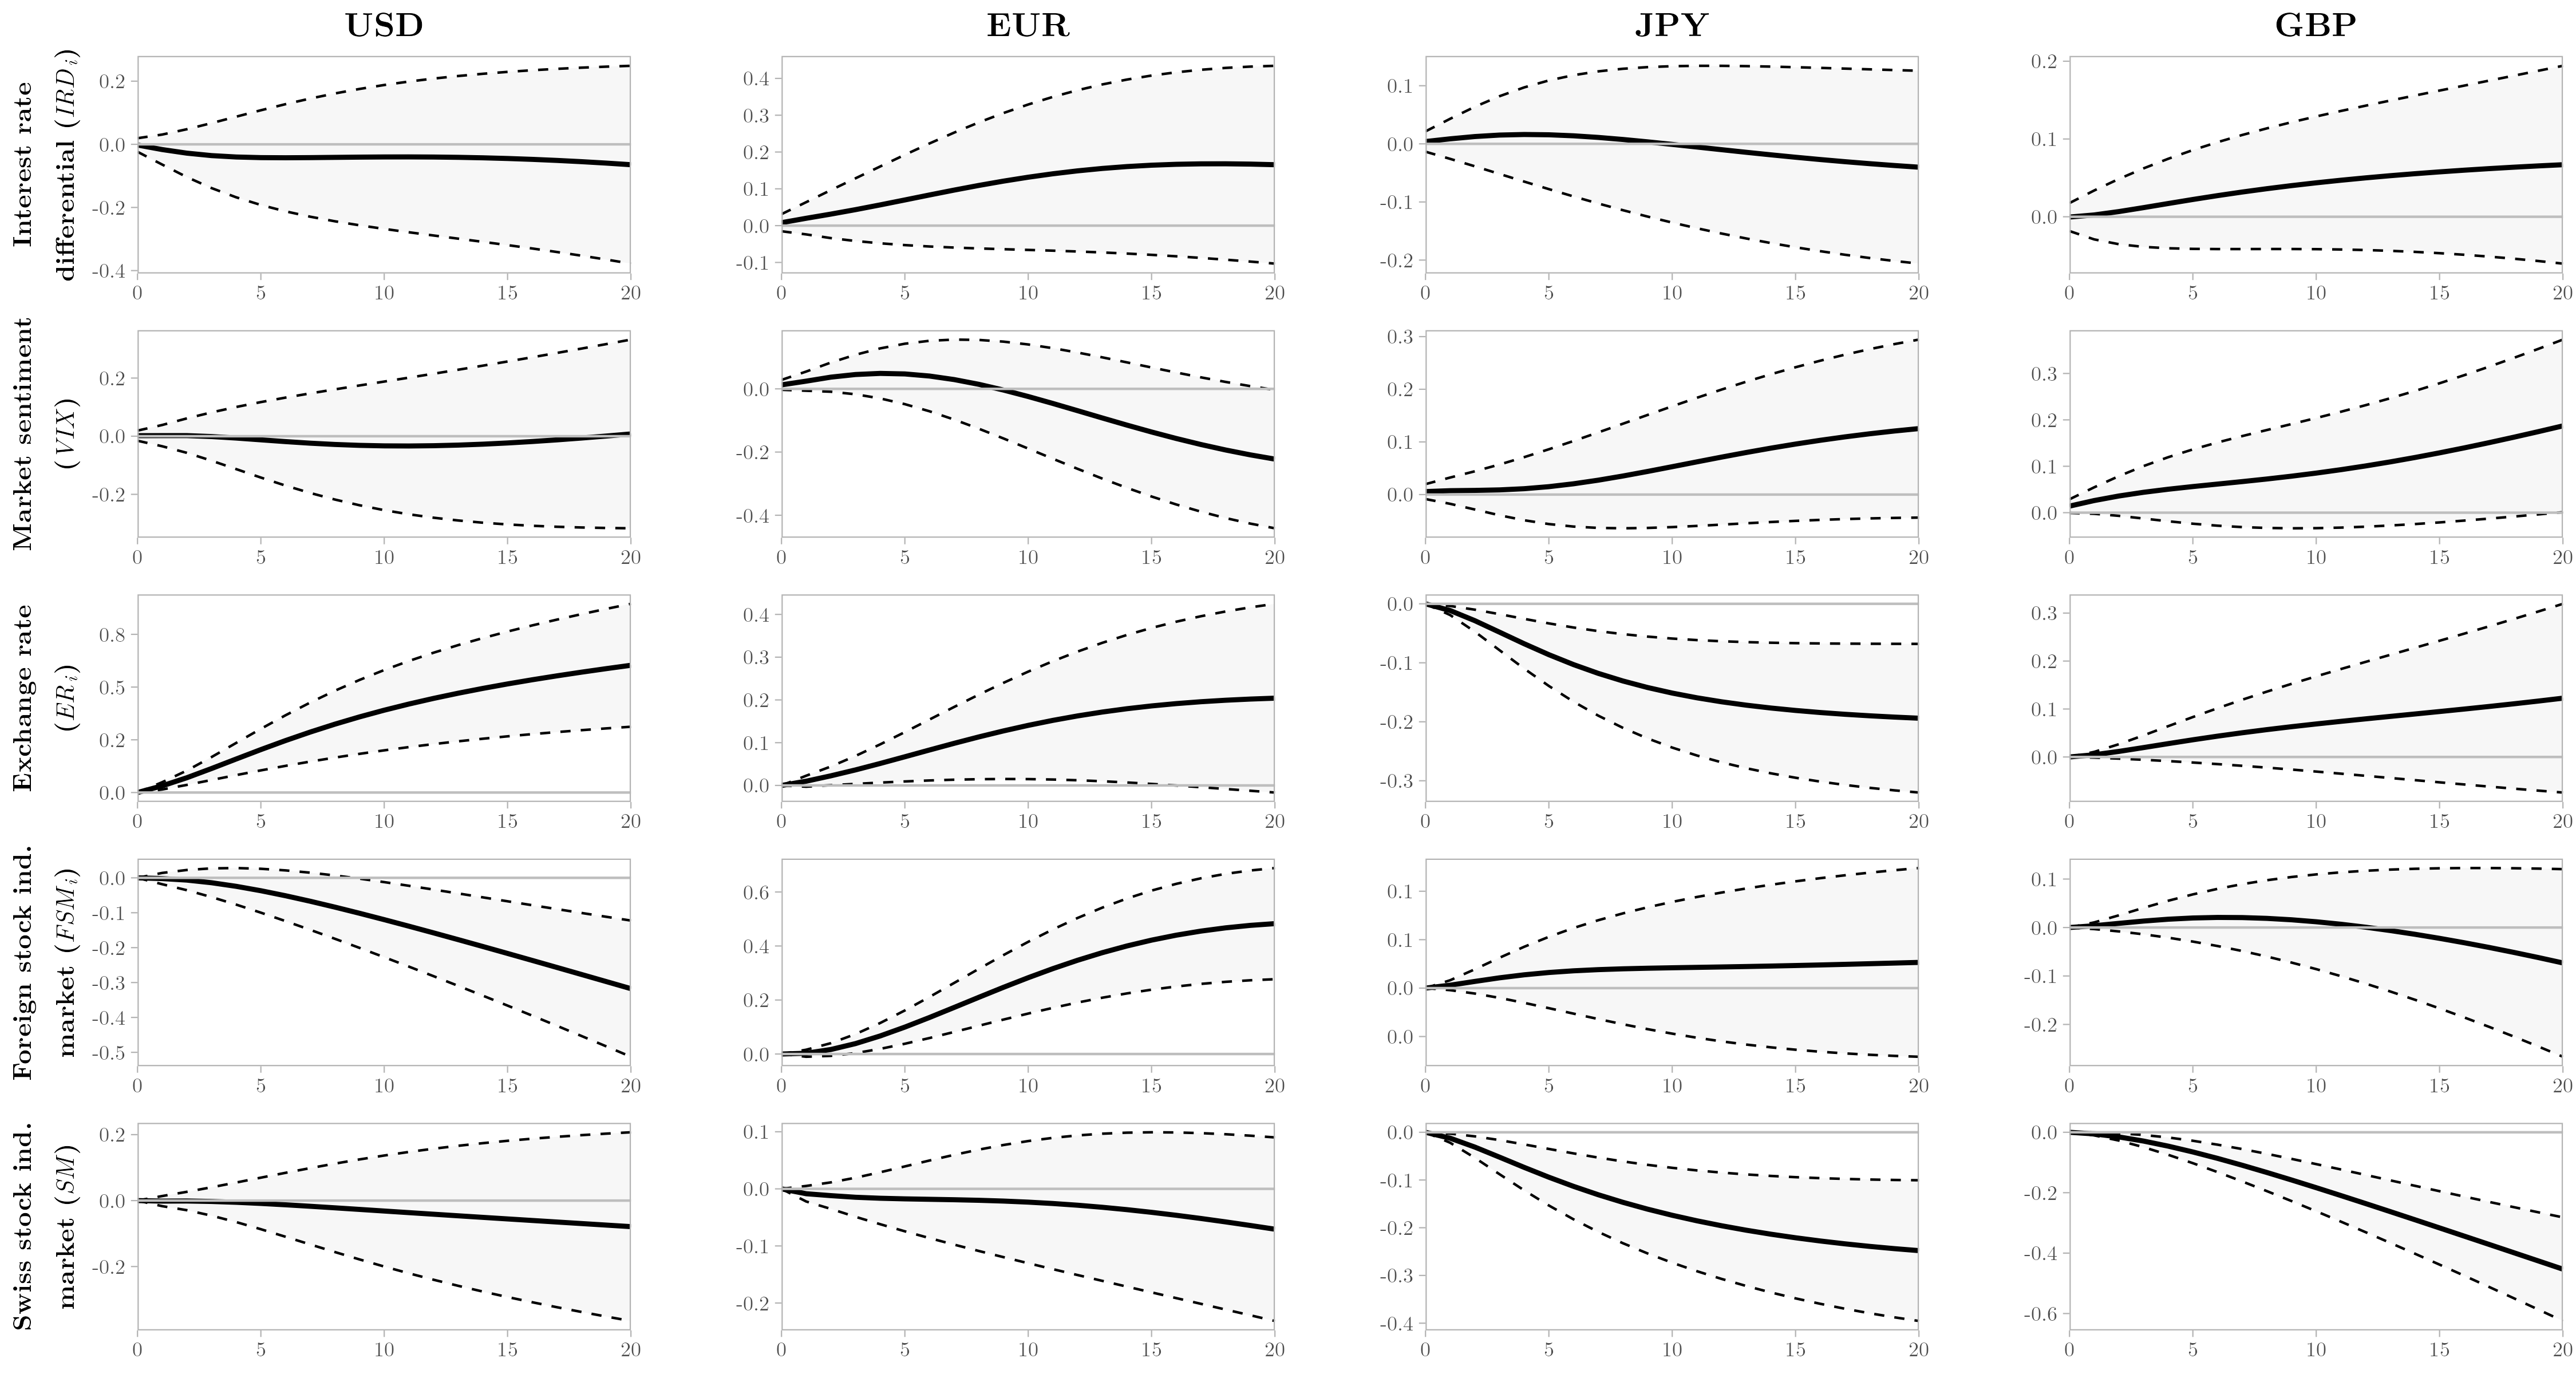
\includegraphics[width=0.99\columnwidth]{figure/gALL_COIRF20_RESP20} 

}

\caption[Responses of Swiss franc carry trade (\textit{CT\textsubscript{i}}) to impulses of financial variables in each target currency model]{Responses of Swiss franc carry trade (\textit{CT\textsubscript{i}}) to impulses of financial variables in each target currency model \newline \scriptsize Notes: Solid line is the cumulative orthogonalized impulse–response function. Dashed lines represent the 95\% lower and upper bounds. We use bootstrap standard errors.}\label{fig:Figure41}
\end{figure}

While there are no statistically significant results for the interest rate differential shock, two different results are found for the impact of a positive shock in the market sentiment on the Swiss franc carry trade. For the EUR model, this shock hinders carry trade. Meanwhile, in the GBP model, evidence for an inverse relationship is found. Both results are found in the long-run (20 weeks ahead the initial shock). While the former confirms the role of the Swiss franc as a funding currency, the latter shows evidence for the role as safe haven.

Regarding the exchange rate shock, a Swiss franc depreciation increases the Swiss franc carry trade activity with all target currencies, except the British pound. This result confirms the carry trade strategy, where the funding currency tends to depreciate while the target currency appreciates. For the USD model, the economic impact is relatively higher than the other exchange rates.

The stock market shocks highlight further the dual role of the Swiss franc. AAfter an increase in the foreign stock market, the USD model negatively impacts the Swiss franc carry trade. Moreover, a bearish stock market may generate better gains than engaging in the carry trade. There is also a statistically significant result for the euro model, where a higher stock activity in the euro area leads to a higher Swiss franc carry trade activity. Both results reinforce the funding role of the Swiss franc in the carry trade activity.

Last but not least, innovations in the Swiss stock market prices decrease the Swiss franc carry trade in both JPY and GBP models. This substitution effect needs to be interpreted cautiously since diversified portfolios to diminish risk are standard practice in the financial market. Another possible explanation is the search for higher yields in the financial markets, not risk mitigation, as indicated by the uncovered equity parity condition (UEP) \autocite{curcuru2014}. Additionally, the argument about the funding role in the relationship between the foreign stock market and carry trade applies here.

\hypertarget{fouronetwo}{%
\subsection{How does the Swiss franc carry trade impact the financial variables in each model?}\label{fouronetwo}}

Figure \ref{fig:Figure42} illustrates the Swiss franc carry trade shock on the financial variables in each target currency analyzed. With the negative interest rate policy, the SNB is extending the role of the Swiss franc as a funding currency. In this scenario, an increase in the Swiss franc carry trade activity is very plausible.

\begin{figure}[!ht]

{\centering 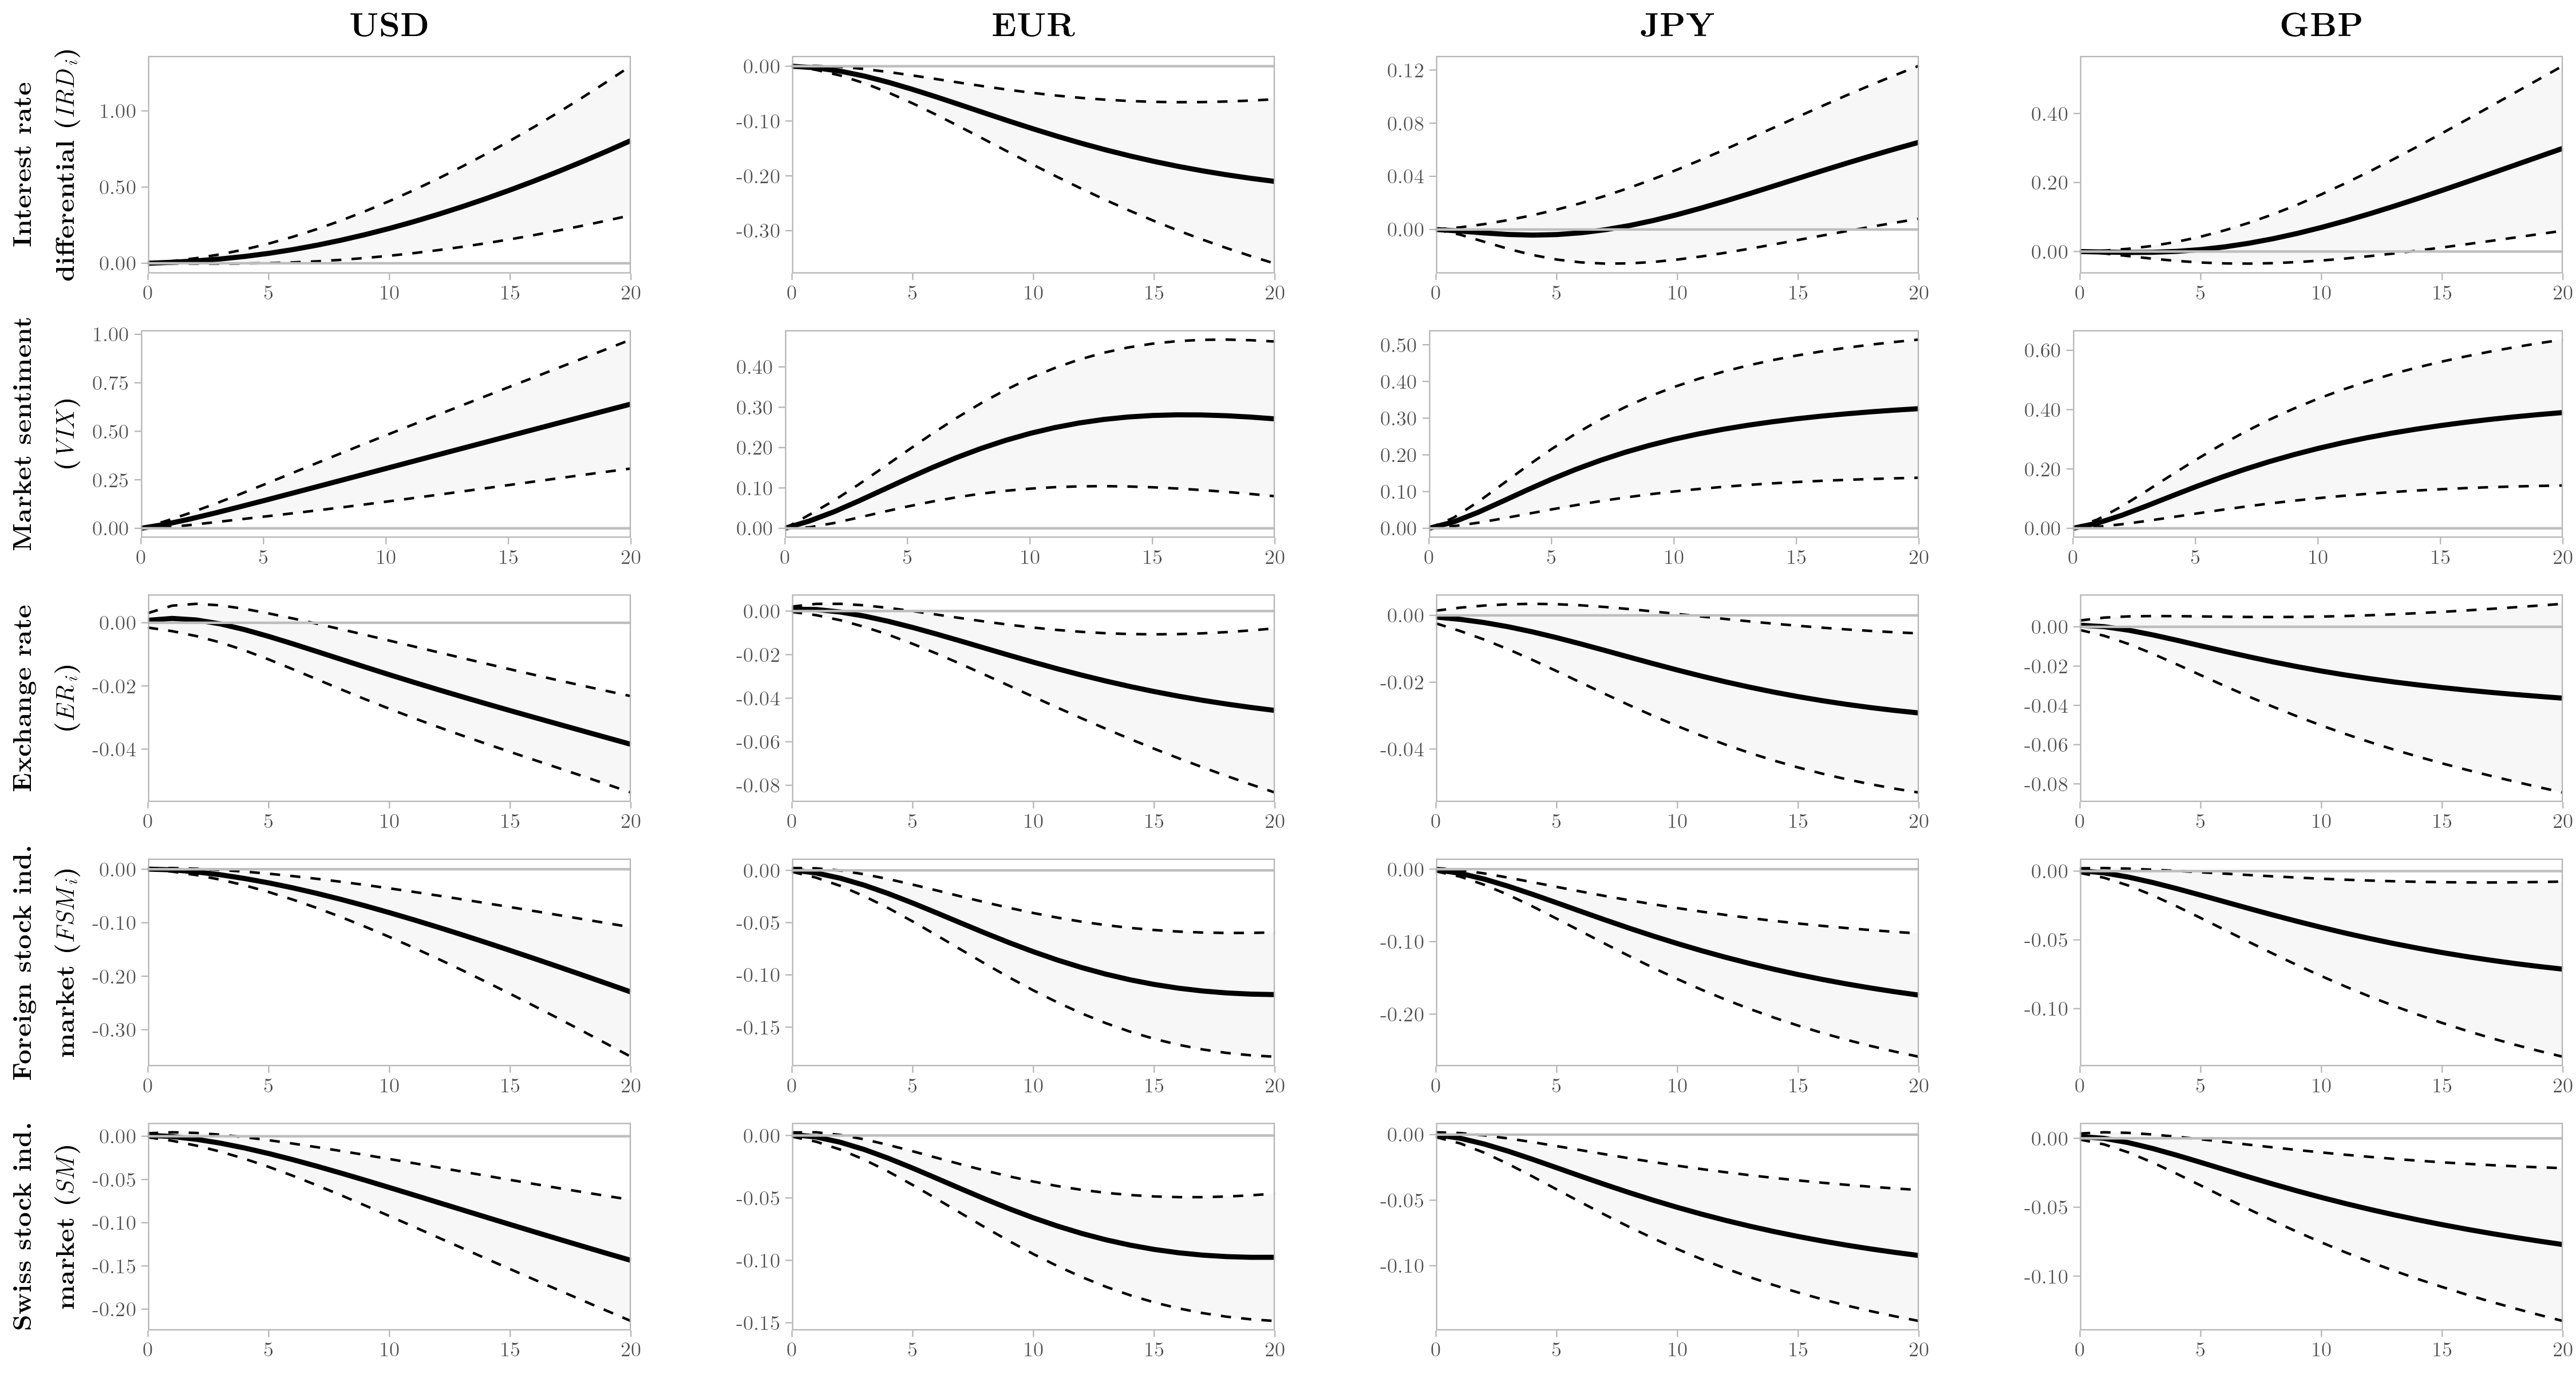
\includegraphics[width=0.99\columnwidth]{figure/gALL_COIRF20} 

}

\caption[Responses of financial variables to impulses of Swiss franc carry trade (\textit{CT\textsubscript{i}}) in each target currency model]{Responses of financial variables to impulses of Swiss franc carry trade (\textit{CT\textsubscript{i}}) in each target currency model \newline \scriptsize Notes: Solid line is the cumulative orthogonalized impulse–response function. Dashed lines represent the 95\% lower and upper bounds. We use bootstrap standard errors.}\label{fig:Figure42}
\end{figure}

While a positive shock on Swiss franc carry trade increases market-driven interest rate differentials for the USD, JPY and GBP models, there is a negative impact on the EUR model. This divergent result may be explained by the different roles of the Swiss franc. While the negative relationship may be related to the safe haven role, the positive impact shows evidence of the funding role.

Following, all models show evidence for a higher market sentiment with a positive shock in the carry trade proxy. By increasing their speculative positions, hedge funds foment global risk, notably with their leveraged activity. In this sense, there is evidence that more speculative Swiss franc activity boosts market risk worldwide.

Particularly, we find evidence for the failure of the UIP in the USD, EUR and JPY models. The Swiss franc carry trade shock leads to a depreciation of both U.S. dollar and euro\footnote{We do not take into account the EUR/CHF peg because it ended in January 2015, while the initial date of the negative interest rate policy in Switzerland is December 18, 2014. \textcite{accominotti2019} investigate the impact of currency regime shifting on the carry trade activity. They suggest that the fixed-to-floating regime switch by the SNB created carry trade losses, starting a global flight-to-safety phenomenon.} (appreciation of the Swiss franc) and to an appreciation of the Japanese yen (depreciation of the Swiss franc). This inverse relationship found in the JPY model, when compared to the results in USD and EUR models, may be related to the different international status of each currency. \textcite{hossfeld2015} classify the euro as a hedge currency, while classifying the Swiss franc, the U.S. dollar and the British pound as safe haven currencies and the Japanese yen as a ``carry funding vehicle''. Therefore, while the results in the USD and EUR models may be related to the Swiss franc as a funding currency, the safe haven role appears in the JPY model.

Conversely, there is a typical result for all models on the impacts of foreign and Swiss stock markets after a positive carry trade shock. These results reveal that institutional investors can move asset prices. Accordingly, this finding resonates with the yen carry trade \autocite{fong2013}. For all models, bearish stock markets result from an increased Swiss franc carry trade activity. More importantly, these results imply that a higher Swiss franc speculative activity is problematic for the financial markets. Jointly, the responses of the market sentiment and both stock market indices indicate a higher systemic risk with the increased Swiss franc carry trade activity. This is also consistent with the adverse side effects of the negative interest rate policy, which have been highlighted by several authors \autocite[see][]{rossi2019}.

\hypertarget{fouronethree}{%
\subsection{Robustness checks}\label{fouronethree}}

The Granger causality tests confirm most of the results found on the impulse-response functions. As shown by Table \ref{tab:Table445}, all variables Granger cause the Swiss franc carry trade in the USD and GBP models. Although not statistically significant in the impulse-response function, the Granger causality test shows that the interest rate differentials impact the carry trade in both USD and GBP models. Some caution regarding the EUR model results is needed since there is no evidence of Granger causality among the variables. In a significant manner, strong evidence is found on the Granger causality of the carry trade proxy on market sentiment and stock market indices in all target currencies (see Table \ref{tab:Table444}). Regarding the UIP failure, only the EUR model shows a statistically significant result.

\begin{table}[!ht]

\caption{\label{tab:Table445}Granger causality tests for the direction $\textit{All variables}$$\rightarrow$$CT_{i}$, p-values}
\centering
\begin{threeparttable}
\begin{tabular}[t]{lcccc}
\toprule
 & $CT_{USD}$ & $CT_{EUR}$ & $CT_{JPY}$ & $CT_{GBP}$\\
\midrule
$IRD_{i}$ & 0.0483** & 0.7511 & 0.9286 & 0.0558*\\
$VIX$ & 0.9823 & 0.2604 & 0.4740 & 0.5320\\
$ER_{i}$ & 0.0015*** & 0.1818 & 0.0241** & 0.0002***\\
$FSM_{i}$ & 0.8945 & 0.3664 & 0.1994 & 0.0034***\\
$SM$ & 0.9624 & 0.3845 & 0.0787* & 0.2506\\
$All$ $variables$ & 0.0311** & 0.5404 & 0.3112 & 0.0097***\\
\bottomrule
\end{tabular}
\begin{tablenotes}[para]
\item \textit{\scriptsize{Notes: }} 
\item \scriptsize{Null hypothesis is that \textit{All variables} ‘does not’ Granger-cause $CT_{i}$. ‘***’, ‘**’, and ‘*’ denote statistical significance at 1\%, 5\%, and 10\%, respectively.} 
\end{tablenotes}
\end{threeparttable}
\end{table}

\begin{table}[!ht]

\caption{\label{tab:Table444}Granger causality tests for the direction $CT_{i}$$\rightarrow$$\textit{All variables}$, p-values}
\centering
\begin{threeparttable}
\begin{tabular}[t]{lccccc}
\toprule
 & $IRD_{i}$ & $VIX$ & $ER_{i}$ & $FSM_{i}$ & $SM$\\
\midrule
$CT_{USD}$ & 0.1881 & 0.0217** & 0.3625 & 0.0656* & 0.0442**\\
$CT_{EUR}$ & 0.0810* & 0.0600* & 0.0648* & 0.0281** & 0.0169**\\
$CT_{JPY}$ & 0.5202 & 0.0395** & 0.7120 & 0.0017*** & 0.0255**\\
$CT_{GBP}$ & 0.8517 & 0.0300** & 0.1296 & 0.0931* & 0.0442**\\
\bottomrule
\end{tabular}
\begin{tablenotes}[para]
\item \textit{\scriptsize{Notes: }} 
\item \scriptsize{Null hypothesis is that $CT_{i}$ ‘does not’ Granger-cause \textit{All variables}. ‘***’, ‘**’, and ‘*’ denote statistical significance at 1\%, 5\%, and 10\%, respectively.} 
\end{tablenotes}
\end{threeparttable}
\end{table}

With the structural forecast-error variance decomposition analysis, we can determine the extent to which each variable may account for the other variable fluctuation. Table \ref{tab:Table43} displays the variance decomposition results for the Swiss franc carry trade (\(CT_i\)).\footnote{In Table \ref{tab:Table43}, Figures \ref{fig:Figure41} and \ref{fig:Figure42} are linked to ``Response = \(CT_i\)'' and ``Impulse = \(CT_i\)'', respectively.} Concerning the financial variables shocks (``Response = \(CT_i\)''), we find that the Swiss franc carry trade is sensitive to the disturbances in the following equations: (i) exchange rate (\(ER_i\)) in the USD model, (ii) foreign stock market index (\(FSM_i\)) in the EUR model and (iii) Swiss stock market index (\(SM\)) in the GBP model. Alike, the decomposition of the impulses of Swiss franc carry trade is presented in Table \ref{tab:Table43} (``Impulse = \(CT_i\)''). For the USD model, results reinforce the argument on the increased systemic risk (\(VIX\)) and the UIP failure (\(ER_{i}\)). Likewise, the linkage between the Swiss carry trade (\(CT_{i}\)) and stock market indices (\(FSM_{i}\) and \(SM\)) is well present in the USD, EUR and JPY models.

\begin{table}[!ht]

\caption{\label{tab:Table43}Structural forecast-error variance decomposition (SFEVD) for each model, in percent}
\centering
\resizebox{\linewidth}{!}{
\fontsize{8}{10}\selectfont
\begin{tabular}[t]{cccccccccccc}
\toprule
\multicolumn{1}{c}{\textbf{ }} & \multicolumn{6}{c}{\textbf{Response $=$ $CT_{i}$}} & \multicolumn{5}{c}{\textbf{Impulse $=$ $CT_{i}$}} \\
\cmidrule(l{3pt}r{3pt}){2-7} \cmidrule(l{3pt}r{3pt}){8-12}
\multicolumn{1}{c}{\textbf{ }} & \multicolumn{6}{c}{\textbf{Impulse $=$}} & \multicolumn{5}{c}{\textbf{Response $=$}} \\
Steps & $IRD_{i}$ & $VIX$ & $CT_{i}$ & $ER_{i}$ & $FSM_{i}$ & $SM$ & $IRD_{i}$ & $VIX$ & $ER_{i}$ & $FSM_{i}$ & $SM$\\
\midrule
\addlinespace[0.3em]
\multicolumn{12}{l}{\textbf{USD model}}\\
\hspace{1em}4 & 0.63 & 0.02 & 92.36 & 6.85 & 0.13 & 0.01 & 0.78 & 4.04 & 0.80 & 2.76 & 2.50\\
\hspace{1em}8 & 0.43 & 0.14 & 86.69 & 11.88 & 0.80 & 0.06 & 2.95 & 9.83 & 5.75 & 10.75 & 10.35\\
\hspace{1em}12 & 0.36 & 0.15 & 83.78 & 13.82 & 1.76 & 0.13 & 6.48 & 14.52 & 10.78 & 18.53 & 18.34\\
\hspace{1em}16 & 0.34 & 0.16 & 81.98 & 14.52 & 2.81 & 0.19 & 10.55 & 18.17 & 14.18 & 24.26 & 24.17\\
\hspace{1em}20 & 0.36 & 0.26 & 80.50 & 14.76 & 3.87 & 0.25 & 14.61 & 21.00 & 16.64 & 28.10 & 28.00\\
\addlinespace[0.3em]
\multicolumn{12}{l}{\textbf{EUR model}}\\
\hspace{1em}4 & 1.22 & 1.33 & 94.38 & 1.13 & 1.71 & 0.23 & 2.08 & 3.03 & 1.67 & 3.36 & 4.07\\
\hspace{1em}8 & 2.02 & 1.21 & 85.32 & 2.41 & 8.86 & 0.17 & 7.00 & 7.47 & 6.31 & 11.67 & 14.46\\
\hspace{1em}12 & 2.45 & 3.16 & 76.00 & 3.12 & 15.11 & 0.16 & 9.25 & 9.36 & 8.20 & 17.91 & 20.80\\
\hspace{1em}16 & 2.47 & 5.67 & 70.54 & 3.28 & 17.81 & 0.23 & 9.23 & 9.44 & 7.88 & 19.84 & 21.67\\
\hspace{1em}20 & 2.38 & 7.15 & 68.72 & 3.24 & 18.12 & 0.39 & 8.30 & 9.16 & 6.79 & 19.34 & 20.11\\
\addlinespace[0.3em]
\multicolumn{12}{l}{\textbf{JPY model}}\\
\hspace{1em}4 & 0.18 & 0.11 & 94.22 & 2.47 & 0.12 & 2.90 & 0.15 & 3.10 & 0.66 & 6.39 & 3.71\\
\hspace{1em}8 & 0.19 & 0.35 & 87.23 & 5.41 & 0.15 & 6.65 & 0.28 & 6.33 & 2.19 & 11.52 & 8.40\\
\hspace{1em}12 & 0.36 & 1.11 & 83.86 & 6.28 & 0.15 & 8.25 & 1.54 & 7.42 & 3.58 & 13.42 & 10.62\\
\hspace{1em}16 & 0.54 & 1.79 & 82.24 & 6.43 & 0.15 & 8.86 & 3.30 & 7.74 & 4.36 & 14.18 & 11.56\\
\hspace{1em}20 & 0.66 & 2.15 & 81.52 & 6.44 & 0.15 & 9.08 & 4.68 & 7.83 & 4.70 & 14.50 & 11.97\\
\addlinespace[0.3em]
\multicolumn{12}{l}{\textbf{GBP model}}\\
\hspace{1em}4 & 0.16 & 1.59 & 96.64 & 0.42 & 0.19 & 1.00 & 0.04 & 3.45 & 1.13 & 1.57 & 2.09\\
\hspace{1em}8 & 0.43 & 1.78 & 91.12 & 1.04 & 0.23 & 5.40 & 0.92 & 7.33 & 2.71 & 3.72 & 5.59\\
\hspace{1em}12 & 0.54 & 2.06 & 84.30 & 1.32 & 0.35 & 11.43 & 2.99 & 8.72 & 3.11 & 4.71 & 7.25\\
\hspace{1em}16 & 0.56 & 2.66 & 77.30 & 1.46 & 0.82 & 17.19 & 4.96 & 8.99 & 2.99 & 4.98 & 7.71\\
\hspace{1em}20 & 0.55 & 3.55 & 70.68 & 1.58 & 1.59 & 22.05 & 6.38 & 8.85 & 2.76 & 4.90 & 7.62\\
\bottomrule
\end{tabular}}
\end{table}

Concerning to other robustness checks, four procedures are computed, as presented in Appendix \ref{appendixc4}. First, the models are estimated using a new ordering of variables, according to the Granger causality tests (Figures \ref{fig:FigureD1} and \ref{fig:FigureD2}). Second, the estimations obtained with the Toda-Yamamoto approach are compared to non-stationary variables (Figures \ref{fig:FigureD3} and \ref{fig:FigureD4}). Third, time dummies are added to verify the accuracy of the estimated models (Figures \ref{fig:FigureD5} and \ref{fig:FigureD6}). Last but not least, we exclude the Swiss franc carry trade in each model to verify the sensitivity of the results (Figures \ref{fig:FigureD7}, \ref{fig:FigureD8}, \ref{fig:FigureD9} and \ref{fig:FigureD10}). Overall, there is no significant change, showing our results are robust to different modeling configurations.

\hypertarget{fourfour}{%
\section{Main conclusions and policy implications}\label{fourfour}}

This paper takes a novel approach to examine the Swiss franc carry trade during the period of negative interest rate policy in Switzerland. Using data from hedge fund positions (i.e., volumes) in the U.S. futures market, we elaborated a new construct of Swiss franc carry trade with four target currencies (U.S. dollar, euro, Japanese yen, and British pound). Each target currency is modeled individually to investigate the behavior of the Swiss franc carry trade. More specifically, we use the formulated model to disentangle the funding currency and safe haven effects embedded in our carry trade proxy.

Our results are uncomplicated to summarize. First, our carry trade proxy captures the funding currency effect of the Swiss franc. In the analysis of the determinants of the Swiss franc carry trade activity, we find that a higher market sentiment leads to an increase in the Swiss franc carry trade in the EUR model, (ii) the foreign stock market index in the EUR model shocks positively the Swiss franc carry trade and (iii) the uncovered interest rate parity (UIP) does not hold for the USD, EUR and JPY models. With negative policy interest rates, the SNB is clearly creating an incentive to foster the Swiss franc as a funding currency in the carry trade strategy. Thus, rather than fulfilling its goal of boosting the Swiss economy, the SNB creates some negative international spillovers.

Second, we also find evidence for the Swiss currency acting as a safe haven currency. The Swiss franc carry trade proxy responds: (i) positively to an increase in the market sentiment in the GBP model and to a Swiss franc depreciation in the USD, EUR and JPY models and (ii) in an inverse manner with the foreign stock market index in the USD model and with the Swiss stock market index in the JPY and GBP models.

Third, we document the violation of the UIP in the USD, EUR and JPY models. By seeking to promote the international competitiveness of Swiss firms and to avoid deflation for the whole economy, the SNB is very keen to depreciate the Swiss franc in relation to other currencies, as seen with the euro peg. Also, with increased funding promoted by the SNB's negative interest rate policy, hedge funds are exploring the invalidity of the UIP to profit.

Fourth, our results suggest that the SNB's negative interest rate policy augments the systemic risk. Evidence for this externality is shown by the linkages between the Swiss franc carry trade activity and financial markets indicators. With all four target currencies, an increased Swiss franc carry trade activity increments the global risk and contracts stock market prices (foreign and Swiss stock market indices). Moreover, we also contribute to the literature of institutional investors by documenting that hedge funds can move asset prices.

More importantly, our results resonate with increased systemic risk with higher speculative activity in Swiss franc. In this sense, our findings are consistent with the existing literature stressing the negative impact of carry trade activities on global financial and monetary risk. Conversely, we should remember that central banks' monetary policies are also more likely to influence carry trade activities when these monetary policies are not coordinated. The SNB's actual negative interest rates policy may have created perverse incentives for more speculation on the Swiss financial market \autocite{rossi2019}. This finding vindicates the view that the SNB should strengthen its remit over asset price regulation in Switzerland. This entails that the SNB would benefit from consolidating its macro-prudential supervision, by setting up new instruments to respond to changing financial variables through new types of monetary and financial condition indices for instance \autocite{guillaumin2017}.

However, more broadly, far-sweeping measures enforced by central banks are needed to avert the risk of financial turmoil and to restore confidence in the global economy. Notably, this is the case with the COVID-crisis that questions the future of currency carry trade activities. Indeed, on the one hand, massive asset-purchasing programs, targeting government bonds in particular, participate in the reduction of the ``safe asset trap'' between bond yields \autocite{reviglio2020}. This is likely to improve global stability through the increase of international supply of safe assets -- warranted by central banks -- with respect to the rise in global demand in search for a flight to safety and liquidity. Specifically, these measures could reduce the demand for safe haven currencies and, consequently, carry trade activities. On the other hand, if future central banks' future measures are non-coordinated or non-cooperative, they could increase exchange rates movements and financial turmoil. In the context of uncertainty characterizing the COVID-crisis, this could further incentivize the Swiss franc carry trade activities.

\begin{savequote}
In one of the various seemingly contradictory aspects of the carry
regime, central bankers seem to have enormous power---their
extraordinary power to create high-powered money, set short-term
interest rates, and strongly influence financial markets with everything
they say---but ultimately they themselves have little latitude to act.
Central banks become merely the agents of carry. Their seeming immense
power is, in reality, mostly illusory.
\qauthor{--- \textcite[\text{p.} 7]{lee2020}}\end{savequote}



\hypertarget{five}{%
\chapter[The political economy of carry trade: The real economy got carried away in Switzerland and Brazil]{\texorpdfstring{The political economy of carry trade: The real economy got carried away in Switzerland and Brazil\footnote{The idea of the political economy of carry trade was given by Guillaume Vallet. I profited from comments and suggestions made by Cédric Tille on an earlier version of this paper. I am grateful for both and remain the sole responsible for the views expressed herein.}}{The political economy of carry trade: The real economy got carried away in Switzerland and Brazil}}\label{five}}

\minitoc 

\hypertarget{fiveone}{%
\section{Introduction}\label{fiveone}}

\noindent Carry trade or currency carry trade is a speculative financial investment. According to \textcite[\text{p.} 40]{frankel2008}, it is an investment strategy of ``going short (betting the foreign exchange value will fall) in a low-interest rate currency'' as the Swiss franc (CHF), ``while simultaneously going long (betting the foreign exchange value will rise) in a high-interest rate currency'' like the Brazilian real (BRL). Each currency in the carry trade will be impacted differently by increases in these bets. Notably, the exchange rate is likely to be affected \autocite{klitgaard2004,fong2013}. By creating erratic movements in the exchange rate, carry trade impacts the real economy of both countries.

This article aims to fill a gap in the carry trade literature by empirically investigating the real economy impacts of the carry trade activity in Switzerland and Brazil. This is done using a Bayesian global vector autoregressive (BGVAR) model, which proxies the global economy. How does carry trade impact both Swiss and Brazilian economies? This addressed question is a novelty in the usual literature on this topic, which focuses on maximizing portfolio returns. The central hypothesis is that there are pervasive effects of this speculative activity.

Theoretically, the carry trade activity should not even exist. According to the uncovered interest rate parity (UIP) hypothesis, exchange rates would neutralize the interest rate differentials between two currencies. In this sense, the UIP states that the carry trade profits would be equal to zero. Nevertheless, as demonstrated several times, the UIP hypothesis is violated in the current international monetary system \autocite[e.g., see the seminal paper by][]{fama1984}. Therefore, carry trade activities are not financially nor economically neutral. Along with their influence on the exchange rates, they also exert a distributive impact and are related to power. Overall, it is a zero-sum game, i.e., one agent's loss is another agent's gain. Such a statement also applies to central banks: managing the impact of carry trade activities cannot occur without entailing risky decisions, which could entail losses for themselves and their economies.

In addition, in order to analyze these relations of power underpinning carry trade activities, a political economy approach is carried out to understand the carry trade effects better. Indeed, funding and target currencies are not affected to the same extent. The power structure in the international monetary system may influence the way carry trade affects individual economies. Specifically, the international hierarchy of currencies confers more or less power to central banks because they could undermine their liberty to implement independent monetary policies \autocite{cohen1998,deconti2013,depaula2017,fritz2018}. Therefore, carry trade activities are related to the power associated with the international status of central banks and currencies. For example, \textcite[\text{p.} 386]{gaulard2012} says that ``{[}t{]}he American monetary creation and the {[}Federal Reserve{]}'s policy of quantitative easing are indeed at the root of an increasing number of capital flows oriented towards emerging countries like Brazil.'' Similarly, ``{[}e{]}xpansionary monetary policies in {[}advanced economies{]} exacerbated the flood of capital to {[}emerging market and developing economies{]}. Investors and speculators were able to engage in the profitable carry trade, borrowing at low interest rates in {[}advanced economies{]} and then investing in {[}emerging market and developing economies{]}, which were characterized by higher interest rates during much of the global crisis.'' \autocite[\text{p.} 199]{grabel2018}

There is a neglected and underestimated political economy of carry trade activities deserving more attention. Political economy is understood here as the academic analysis of politically and socially embedded economic activities, resting on the idea to place power relations at the core of these activities. Power is associated with both structures and interactions between actors, the latter encompassing the States and individual actors \autocite{strange1994,may1996}. Within the carry trade context, this implies focusing on the States, but also on central banks and on private investors of different kinds (for example, dealers/intermediaries, asset managers, leveraged funds, investment banks). International organizations are also vital in this scheme. For example, the International Monetary Fund's view on capital controls changed significantly after the 2008 global financial crisis. As pointed out by \textcite[\text{p.} 213]{grabel2018}, ``{[}t{]}he rebranding of controls has also been facilitated by the fact that carry trade pressures in some {[}advanced economies{]} caused central bankers to reconsider their long-held opposition to currency interventions and even to capital controls.''

The political economy is crucial to the investigation of carry trade activities since it identifies the different relations of power associated with international monetary transactions. This framework also challenges the dichotomies often used to delve into this topic. For instance, there is a binary rationale about developed and developing/emerging countries or about funding and investing currencies. Though relevant to some extent, such dichotomies do not reflect the complexity of carry trade activities and their relations of power. The complexity of these power relations between economic actors overlaps the current understanding of carry trade activities.

There are two levels of power conflict in the political economy approach to the carry trade. First, internationally, currencies from developed countries are preferred to currencies from developing countries, as illustrated by the currency hierarchy. Second, domestically, central banks accept the risk of the carry trade activity following the pressure of actors from the financial sector. As proposed by \textcite[\text{p.} 57]{schoenmaker2011}`s financial trilemma, ``financial stability, financial integration and national financial policies are incompatible.'' Furthermore, democracy and national sovereignty questions appear regarding central banks' handling of the carry trade.

In sum, the impacts of the carry trade activities on the real economy have been overlooked. Notably, the paper contributes to a better understanding of these impacts by investigating the cases of two notorious funding and target currencies, the Swiss franc and the Brazilian real, respectively. There is evidence that the carry trade negatively impacts the real economy. Our interpretation is that carry trade crowds out real investment, along with the distortions on the exchange rate. Nevertheless, these impacts do not present a high economic magnitude, also being conditional to the periodicity of the estimated model. Additionally, a broader discussion of these impacts is possible with the political economy approach. The remainder is organized as follows. Section \ref{fivetwo} gives a data overview and describes the econometric framework. The links between the real economy and the carry trade activities are explored with the transmission of structural shocks in section \ref{fivethree}. The main conclusions are drawn in section \ref{fivefour}.

\hypertarget{fivetwo}{%
\section{Data overview and econometric framework}\label{fivetwo}}

This section describes the data set created for the empirical assessment of the carry trade effects on the Swiss and Brazilian real economy. Succeeding the data description, there is the demonstration of the econometric framework with a general description of the Bayesian global vector autoregressive (BGVAR) model. Next, a subsection discusses both the implemented model setup and the pre-testing procedure.

\hypertarget{fivetwoone}{%
\subsection{Data}\label{fivetwoone}}

The world economy is proxied by 21 countries and one regional aggregate, the euro area (see Table \ref{tab:Table51}). This makes a total of 22 units. Additionally, the main currency pairs available on the CFTC public database are present. Most importantly, according to the \textcite{worldbank2021}, these countries account for about 84\% of global nominal output (GDP, current USD)\footnote{The code for the indicator used is ``NY.GDP.MKTP.CD''.} averaged over the years 2014 and 2019.

\begin{table}[!ht]

\caption{\label{tab:Table51}Country coverage}
\centering
\begin{threeparttable}
\resizebox{\linewidth}{!}{
\begin{tabular}[t]{>{\centering\arraybackslash}p{3cm}>{\raggedright\arraybackslash}p{11cm}}
\toprule
\multirow{3}{*}[0pt]{CFTC countries} & Australia (AU), Brazil (BR), Canada (CA), Switzerland(CH), United Kingdom (GB), Japan (JP), Mexico (MX), New Zealand (NZ), Russia (RU), Euro area (U2)$^*$, United States (US)\\
\addlinespace
\multirow{3}{*}[0pt]{Global economy} & China (CN), Czech Republic (CZ), Denmark (DK), Hungary (HU), India (IN), Korea, Rep. (KR), Norway (NO), Poland (PL), South Africa (ZA), Sweden (SE), Turkey (TR)\\
\bottomrule
\end{tabular}}
\begin{tablenotes}[para]
\item \footnotesize{$Notes$: Abbreviations follow the two-digit codes provided by IMF's database International Financial Statistics (IFS). South Africa (ZA) is excluded from the CFTC group due to lack of data.}

\item[*] \footnotesize{Changing composition.}
\end{tablenotes}
\end{threeparttable}
\end{table}

Table \ref{tab:Table52} lists all variables included in the estimated models.




\begin{table}[!ht]

\caption{\label{tab:Table52}Data description}
\centering
\resizebox{\linewidth}{!}{
\fontsize{8}{10}\selectfont
\begin{threeparttable}
\begin{tabular}[t]{c>{\raggedright\arraybackslash}p{6cm}>{\centering\arraybackslash}p{3cm}cccccccl}
\toprule
\multicolumn{3}{c}{ } & \multicolumn{8}{c}{Model} \\
\cmidrule(l{3pt}r{3pt}){4-11}
\multicolumn{3}{c}{\em{ }} & \multicolumn{4}{c}{\em{Quarterly}} & \multicolumn{4}{c}{\em{Monthly}} \\
\cmidrule(l{3pt}r{3pt}){4-7} \cmidrule(l{3pt}r{3pt}){8-11}
Variable & Definition & Source & (1) & (2) & (3) & (4) & (5) & (6) & (7) & (8)\\
\midrule
$GDP$ & Gross domestic product$\textsuperscript{*}$ & OECD & $\bullet$ & $\bullet$ &  &  &  &  &  & \\
$C$ & Final consumption expenditure$\textsuperscript{*}$ & OECD &  &  & $\bullet$ & $\bullet$ &  &  &  & \\
$GFCF$ & Gross fixed capital formation$\textsuperscript{*}$ & OECD &  &  & $\bullet$ & $\bullet$ &  &  &  & \\
$X$ & Exports of goods and services$\textsuperscript{*}$ & OECD &  &  & $\bullet$ & $\bullet$ & $\bullet$ & $\bullet$ & $\bullet$ & $\bullet$\\
$M$ & Imports of goods and services$\textsuperscript{*}$ & OECD &  &  & $\bullet$ & $\bullet$ & $\bullet$ & $\bullet$ & $\bullet$ & $\bullet$\\
\multirow{2}{*}[0pt]{$RES$} & Official reserve assets and other foreign currency assets$\textsuperscript{*}$ & \multirow{2}{*}[0pt]{IMF} & \multirow{2}{*}[0pt]{$\bullet$} & \multirow{2}{*}[0pt]{$\bullet$} & \multirow{2}{*}[0pt]{$\bullet$} & \multirow{2}{*}[0pt]{$\bullet$} & \multirow{2}{*}[0pt]{$\bullet$} & \multirow{2}{*}[0pt]{$\bullet$} & \multirow{2}{*}[0pt]{$\bullet$} & \multirow{2}{*}[0pt]{$\bullet$}\\
$IR$ & Policy interest rate & BIS & $\bullet$ & $\bullet$ & $\bullet$ & $\bullet$ & $\bullet$ & $\bullet$ & $\bullet$ & $\bullet$\\
$ER$ & Nominal exchange rate$\textsuperscript{*}$ & BIS & $\bullet$ & $\bullet$ & $\bullet$ & $\bullet$ & $\bullet$ & $\bullet$ & $\bullet$ & $\bullet$\\
$EQ$ & Equity (share) prices$\textsuperscript{*}$ & OECD & $\bullet$ & $\bullet$ & $\bullet$ & $\bullet$ & $\bullet$ & $\bullet$ & $\bullet$ & $\bullet$\\
\multirow{2}{*}[0pt]{$NP$} & Net (long minus short) positions as a share of open interest contracts (carry trade proxy) & \multirow{2}{*}[0pt]{CFTC} & \multirow{2}{*}[0pt]{$\bullet$} & \multirow{2}{*}[0pt]{$\bullet$} & \multirow{2}{*}[0pt]{$\bullet$} & \multirow{2}{*}[0pt]{$\bullet$} & \multirow{2}{*}[0pt]{$\bullet$} & \multirow{2}{*}[0pt]{$\bullet$} & \multirow{2}{*}[0pt]{$\bullet$} & \multirow{2}{*}[0pt]{$\bullet$}\\
$VIX$ & CBOE Volatility Index (VIXCLS)$\textsuperscript{*}$ & FRED & $\bullet$ &  & $\bullet$ &  & $\bullet$ &  & $\bullet$ & \\
\multirow{2}{*}[0pt]{$GCF$} & Global common factor estimated from world-wide cross section of risky asset prices & \textcite{miranda-agrippino2021a} &  & \multirow{2}{*}[0pt]{$\bullet$} &  & \multirow{2}{*}[0pt]{$\bullet$} &  & \multirow{2}{*}[0pt]{$\bullet$} &  & \multirow{2}{*}[0pt]{$\bullet$}\\
$IP$ & Industrial production excluding construction$\textsuperscript{*}$ & OECD &  &  &  &  &  &  & $\bullet$ & $\bullet$\\
\bottomrule
\end{tabular}
\begin{tablenotes}[para]
\item \footnotesize{$Notes$: See Table \ref{tab:TableSD00} in Appendix \ref{appendixd} for more details.}

\item[*] \footnotesize{Variables in logarithmic transform.}
\end{tablenotes}
\end{threeparttable}}
\end{table}

In line with \textcite{fong2013}, the carry trade proxy is restricted to the category leveraged funds in the CFTC platform. For more details, see the report Traders in Financial Futures \autocite{commodityfuturestradingcommission2021}. Furthermore, as presented by \textcite[\text{p.} 321]{brunnermeier2008}, the carry trade proxy (\(NP\)) is given by ``the net (long minus short) futures position of noncommercial traders in the foreign currency, expressed as a fraction of total open interest of all traders'':
\begin{equation}
\text{Net positions} = \frac{\text{Long positions} - \text{Short positions}}{\text{Open interest}}
\end{equation}

Eight data sets are structured by collecting the largest sample possible for each country (Switzerland and Brazil). As detailed in Table \ref{tab:Table521}, models (1) to (4) models are estimated with quarterly data, while models (5) to (8) use monthly data.

\begin{table}[!ht]

\caption{\label{tab:Table521}Time span for each model}
\centering
\begin{threeparttable}
\begin{tabular}[t]{ccccc}
\toprule
Country & Period & Observations & Global risk & Models\\
\midrule
\addlinespace[0.3em]
\multicolumn{5}{l}{\textbf{Quarterly data}}\\
 & 2006-Q2 to 2021-Q2 & 61 & $VIX$ & (1), (3)\\

\multirow{-2}{*}{\centering\arraybackslash \hspace{1em}Switzerland} & 2006-Q2 to 2019-Q1 & 52 & $GCF$ & (2), (4)\\

\hspace{1em}Brazil & 2012-Q2 to 2021-Q2 & 37 & $VIX$ & (1), (3)\\

\addlinespace[0.3em]
\multicolumn{5}{l}{\textbf{Monthly data}}\\
 & 2006-06 to 2021-07 & 182 & $VIX$ & (5)\\

\multirow{-2}{*}{\centering\arraybackslash \hspace{1em}Switzerland} & 2006-06 to 2019-04 & 155 & $GCF$ & (6)\\

 & 2014-01 to 2021-07 & 91 & $VIX$ & (5), (7)\\

\multirow{-2}{*}{\centering\arraybackslash \hspace{1em}Brazil} & 2014-01 to 2019-04 & 64 & $GCF$ & (6), (8)\\
\bottomrule
\end{tabular}
\begin{tablenotes}[para]
\item \footnotesize{$Notes$: Models (2) and (4) are not estimated for Brazil due to a lack of data, which leads to a sample of 27 observations. For Switzerland, models (7) and (8) are not estimated because there is no monthly data for industrial production.}

\end{tablenotes}
\end{threeparttable}
\end{table}

As detailed in Appendix \ref{appendixd00}, the last available data in each period is used for the CFTC data. Moreover, the period-end approach is used for the daily variables. The primary data issue is related to Brazil's lack of CFTC data. To achieve a continuous sample, the data sets for Brazil must start in 2012-Q2 and January 2014 for quarterly and monthly models, respectively. Furthermore, the time restriction to February 2021 is due to data availability, which avoids a possible selection bias problem. Therefore, the estimations do not fully account for the COVID crisis, considering March 2021 as the worst economic moment so far.

\hypertarget{fivetwotwo}{%
\subsection[The Bayesian global vector autoregressive model]{\texorpdfstring{The Bayesian global vector autoregressive model\footnote{This subsection follows closely the econometric framework presented in \textcite[\text{pp.} 169-171]{feldkircher2016}.}}{The Bayesian global vector autoregressive model}}\label{fivetwotwo}}

As originally formulated by \textcite[\text{p.} 159]{pesaran2004}, a global vector autoregressive model (GVAR) is ``an operational framework for global macroeconomic modeling.'' More specifically, \textcite[\text{p.} 169]{feldkircher2016} summarize that

\begin{quote}
{[}i{]}n principle, it comprises two layers via which the model is able to capture cross-country spillovers. In the first layer, we estimate separate time series models for each country contained in the global model. This takes cross-country differences of the economies appropriately into account since we do not impose any kind of homogeneity e.g., in a panel VAR. In the second layer, the country models are stacked to yield a global model that is able to trace the spatial propagation of a shock as well as its time dynamics.
\end{quote}

Algebraically, the first layer comprises the individual country models in an augmented VAR model (VARX\(^*\)) specification. For example, VARX\(^*\)(1,1), for \(t \in 1, ..., T\) and \(i \in 0, ..., N\)
is determined by
\begin{equation}
x_{i,t} = a_{i0} + a_{i1}t + \psi_{i1}x_{i,t-1} + \Lambda_{i0}x_{i,t}^{\ast} + \Lambda_{i0}x_{i,t-1}^{\ast} + \varepsilon_{i,t},
\label{eq:51}
\end{equation}

\noindent where \(x_{i,t}\) is a \(k_i \times 1\) matrix at time \(t\) in country \(i\). There are also coefficients for a constant (\(a_{i0}\)) and a deterministic trend (\(a_{i1}\)). In addition, \(\psi_{i1}\) gives the \(k_i \times k_i^\ast\) matrix of dynamic coefficients for the lagged endogenous variables in country \(1\). Weakly exogenous variables (\(x_{i,t}^{\ast}\), \(k_i^* \times 1\) matrix) are given by
\begin{equation}
x_{i,t}^{\ast} = \sum_{j\neq i}^N\omega_{ij}x_{j,t},
\label{eq:52}
\end{equation}

\noindent where \(\omega_{ij}\) denotes bilateral weights between countries \(i\) and \(j\). Generally, trade weights are used in the literature, but financial flows are also present. \textcite{eickmeier2015} do not find differences in their results by testing different weighting schemes. Additionally, \textcite{feldkircher2016} show that trade weights present good fitness in a sensitivity analysis under a Bayesian GVAR model. In this sense, trade weights\footnote{See the trade weight matrix in Table \ref{tab:TableSD0} in Appendix \ref{appendixd0}.} are employed in the estimated model presented in the following sections. With variance-covariance matrix \(\Sigma_{\varepsilon,j}\), the usual vector white noise process is determined by \(\varepsilon_{i,t} \sim \mathcal{N} (0,\Sigma_{\varepsilon,i})\).

\begin{quote}
Several facts arise from \eqref{eq:51}. First, note that weakly exogenous variables enter the model contemporaneously. Since bilateral weights \(\omega_{ij}\) are assumed to be exogenous and fixed, weakly exogenous variables simply resemble a function of \(x_t\) and are thus endogenously determined within the global system. {[}\ldots{]} Second, note that if \(\Lambda_{i0} = \Lambda_{i1} = 0\) the VARX\(^*\) collapses to a standard first-order VAR model featuring a deterministic time trend. \autocite[\text{p.} 169]{feldkircher2016}
\end{quote}

In the second layer, country-specific VARX models are solved simultaneously for all domestic variables by stacking \(x_{i,t}\) and \(x_{i,t}^{\ast}\) to retrieve a \((k_i + k_i^*)\)-dimensional vector \(z_{i,t} = (x_{i,t}^{'}, x_{i,t}^{'\ast})'\). The model in Equation \eqref{eq:51} can be rewritten by gathering all contemporaneous terms on the left-hand side, as shown by
\begin{equation}
A_iz_{i,t} = a_{i0} + a_{i1}t + B_iz_{i,t-1} + \varepsilon_{i,t},
\label{eq:53}
\end{equation}

\noindent with \(A_i = (I_{k_i}, -\Lambda_{i0})\) and \(B_i = (\psi_{i1}, \Lambda_{i1})\) being \((k_i + k_i^*)\) matrices. In terms of a global vector, \(z_{i,t}\) is rewritten by using a \((k_i + k_i^*) \times k\) link matrix \(W_i\), where \(k = \Sigma_{i=0}^Nk_i\) is the number of endogenous variables in the global system. Given that all endogenous variables in the system are gathered in the \(k\)-dimensional vector \(x_t = (x_{0,t}', ..., x_{N,t}')\), \(z_{i,t}\) can be written as, with the use of \eqref{eq:52},
\begin{equation}
z_{i,t} = W_ix_t.
\label{eq:54}
\end{equation}

Therefore, Equation \eqref{eq:51} is used to obtain the country model in terms of the global vector, as shown by
\begin{equation}
A_iW_ix_t = a_{i0} + a_{i1}t + B_iW_ix_{t-1} + \varepsilon_{i,t}.
\label{eq:55}
\end{equation}

Matrices \(A_iW_i\) and \(B_iW_i\) for all countries stacked gives
\begin{equation}
Gx_t = a_{0} + a_{1}t + Hx_{t-1} + \varepsilon_{t},
\label{eq:56}
\end{equation}

\noindent where \(a_0 = (a_{00}', ..., a_{N0}')'\), \(a_1 = (a_{01}', ..., a_{N1}')'\), \(G = [(A_0W_0)', ..., (A_NW_N)']\), \(H = [(B_0W_0)', ..., (B_NW_N)']\) and \(\varepsilon_t = (\varepsilon_{0,t}', ..., \varepsilon_{N,t}')' \sim \mathcal{N} (0,\Sigma_\varepsilon)\). With \(\Sigma_{\varepsilon,i}\) on the main diagonal, \(\Sigma_\varepsilon\) is assumed a block-diagonal matrix. The global vector autoregressive model is derived by multiplying from the left by \(G^{-1}\):
\begin{equation}
  \begin{aligned}
x_t 
& = G^{-1}a_{0} + G^{-1}a_{1}t + G^{-1}Hx_{t-1} + G^{-1}\varepsilon_{t} \\
& = b_0 + b_1t + Fx_{t-1} + e_t,
  \end{aligned}
\label{eq:57}
\end{equation}

\noindent where \(F\) denotes the \(k \times k\) companion matrix and \(e_t = \sim \mathcal{N} (0,\Sigma_e)\) considering \(\Sigma_e = G^{-1} \Sigma_eG^{-1'}\). Thence, contemporaneous relationships between countries are established with matrix \(G\). By being close to a simple VAR(1), Equation \eqref{eq:57} allows the implementation of standard methods (e.g., impulse response analysis). By excluding the eigenvalues of the \(F\)-matrix larger than 1.05 in the estimated model in the following section, shocks are restricted to ``no permanent impact on the system in the very long-run.'' \autocite[\text{p.} 170]{feldkircher2016} This condition is possible by imposing the discard of posterior draws that exceed this limit.

The importance of the Bayesian approach to estimate the GVAR model is well explained by \textcite[\text{p.} 3]{feldkircher2020}, adapted to the equations demonstrated here:

\begin{quote}
While the GVAR modeling approach imposes parsimony by restricting the coefficients related to other countries' endogenous variables to be driven by economic weights (see Eq. \eqref{eq:52}), the remaining number of parameters in Eq. \eqref{eq:57} is still typically higher than the number of available observations. This calls for Bayesian shrinkage priors that effectively deal with this problem by shrinking the parameter space toward some stylized prior model.
\end{quote}

\hypertarget{fivetwothree}{%
\subsection{Model setup and pre-testing}\label{fivetwothree}}

There are three priors available to choose in the \texttt{R} package \texttt{BGVAR}\footnote{Version 2.4.1 is used.} \autocite{bock2021}: Stochastic Search Variable Selection prior - SSVS \autocite{george1993,george2008}, Non-conjugate Minnesota prior - MN \autocite{litterman1986,koop2010}, and Normal-Gamma prior - NG \autocite{huber2019}. Following the same logic in \textcite[\text{p.} 170]{feldkircher2016}, the former is chosen because it considers formally ``uncertainty about variable choice into account''. \textcite[\text{Appendix A, pp.} 11-12]{feldkircher2020} provide detailed information about this prior setup and the Markov chain Monte Carlo algorithm. Technically, the main features of the SSVS prior implemented on \texttt{BGVAR} is explained in-depth by the package's authors in \textcite[\text{pp.} 4-6]{bock2020}\footnote{See also \textcite[\text{pp.} 1377-1378]{cuaresma2016} and \textcite[\text{pp.} 170-171]{feldkircher2016}.}.

Also, more details on the model setup is supplied in Appendix \ref{appendixd1}, which also presents the full list of variables for each country model (for Switzerland, Tables \ref{tab:TableSDQ1} to \ref{tab:TableSD11}; for Brazil, Tables \ref{tab:TableSDQ5} to \ref{tab:TableSD15}). In addition, the number of lags imposed in the estimated model equals to one (1) for all endogenous and weakly exogenous variables. Regarding the draws and burn-ins, they are equal to 20,000 and 35,000, respectively. ``To ensure that the MCMC estimation has converged, a high-number of burn-ins is recommended'' \autocite[\text{p.} 9]{bock2020}. Besides a constant, each country model has a deterministic trend as well. In particular, the model is estimated with stochastic volatility, as developed by \textcite{kastner2016}, which is important for two main reasons:

\begin{quote}
There are several reasons why one may want to let the residual variances change over time. First and foremost, data frequently used in macroeconometrics contain volatile periods, such as severe recessions and gradual recoveries. Hence accounting for time variation can considerably improve the fit of the model \autocite{primiceri2005,sims2006,dovern2016,huber2016}. Second, the specification implemented in this library nests the homoskedastic case. \autocite[\text{p.} 10]{bock2020}
\end{quote}

To model global risk, the setup follow the setup put forward by \textcite{georgiadis2015}, \textcite{mohaddes2019} and \textcite{feldkircher2020}. Figure \ref{fig:Figure510} illustrates the model setup.

\begin{figure}[!ht]

{\centering \includegraphics[width=0.99\columnwidth]{figure/Setup} 

}

\caption[GVAR setup with global risk modeled separately ($VIX$ or $GCF$)]{GVAR setup with global risk modeled separately ($VIX$ or $GCF$) \newline \scriptsize Notes: The variable $NP$ for Brazil is not included in the models for Switzerland. Similarly, $NP$ for Russia and South Africa are also excluded from these models. The reason is the lack of data.}\label{fig:Figure510}
\end{figure}

Before continuing to the results of the estimated models, some pre-testing is needed. The first test is \textcite{geweke1992}'s convergence diagnostic, which ``assesses practical convergence of the MCMC algorithm.'' \autocite[\text{p.} 11]{bock2020}

\begin{quote}
In a nutshell, the diagnostic is based on a test for equality of the means of the first and last part of a Markov chain (by default we use the first 10\% and the last 50\%). If the samples are drawn from the stationary distribution of the chain, the two means are equal and Geweke's statistic has an asymptotically standard normal distribution. The test statistic is a standard Z-score: the difference between the two sample means divided by its estimated standard error. The standard error is estimated from the spectral density at zero and so takes into account any autocorrelation. \autocite[\text{p.} 11]{bock2020}
\end{quote}

As shown by the results in Table \ref{tab:Table5Z}, the Geweke statistic is very low for all models. For example, regarding model 1 for Switzerland, 8.62\% of the variables' z-values exceed the 1.96 threshold. Therefore, only a very small fraction of all coefficients do not converge.

\begin{table}[!ht]

\caption{\label{tab:Table5Z}Convergence diagnostics, Geweke statistic}
\centering
\resizebox{\linewidth}{!}{
\begin{tabular}[t]{ccccccccc}
\toprule
\multicolumn{1}{c}{ } & \multicolumn{8}{c}{Model} \\
\cmidrule(l{3pt}r{3pt}){2-9}
Country & (1) & (2) & (3) & (4) & (5) & (6) & (7) & (8)\\
\midrule
Switzerland & 8.62\% & 6.9\% & 11.06\% & 14.23\% & 14.13\% & 14.55\% &  & \\
Brazil & 10.53\% &  & 12.2\% &  & 10.59\% & 8.12\% & 9.68\% & 8.41\%\\
\bottomrule
\end{tabular}}
\end{table}

Second, an F-test for serial autocorrelation in the residuals is analyzed. As demonstrated by the results in Table \ref{tab:Table53CH} for Switzerland and Table \ref{tab:Table53BR} for Brazil, the null hypothesis of no serial correlation cannot be rejected for a large number of equations' residuals. Regarding the speficities of the test performed,

\begin{quote}
{[}i{]}t is the F-test of the familiar Lagrange Multiplier (LM) statistic \autocites*[see Godfrey][]{godfrey1978,godfrey1978a}, also known as the 'modified LM' statistic. The null hypothesis is that \(rho\), the autoregressive parameter on the residuals, equals 0 indicating absence of serial autocorrelation. For higher order serial correlation, the null is that all \(rho\)'s jointly are 0. The test is implemented as in Vanessa Smith's and Alessandra Galesi's ''GVAR toolbox 2.0 User Guide'', page 129. \autocite[\text{p.} 34]{bock2021}
\end{quote}

\begin{table}[!ht]

\caption{\label{tab:Table53CH}First order serial autocorrelation of cross-country residuals (F-test) for Switzerland}
\centering
\resizebox{\linewidth}{!}{
\begin{tabular}[t]{ccccccc}
\toprule
\multicolumn{1}{c}{ } & \multicolumn{6}{c}{Model} \\
\cmidrule(l{3pt}r{3pt}){2-7}
p-values & (1) & (2) & (3) & (4) & (5) & (6)\\
\midrule
>0.1 & 70 (60.87\%) & 75 (65.22\%) & 107 (60.11\%) & 119 (66.85\%) & 64 (46.38\%) & 74 (53.62\%)\\
0.05-0.1 & 5 (4.35\%) & 9 (7.83\%) & 21 (11.8\%) & 15 (8.43\%) & 10 (7.25\%) & 10 (7.25\%)\\
0.01-0.05 & 12 (10.43\%) & 10 (8.7\%) & 19 (10.67\%) & 22 (12.36\%) & 18 (13.04\%) & 15 (10.87\%)\\
<0.01 & 28 (24.35\%) & 21 (18.26\%) & 31 (17.42\%) & 22 (12.36\%) & 46 (33.33\%) & 39 (28.26\%)\\
\bottomrule
\end{tabular}}
\end{table}

\begin{table}[!ht]

\caption{\label{tab:Table53BR}First order serial autocorrelation of cross-country residuals (F-test) for Brazil}
\centering
\resizebox{\linewidth}{!}{
\begin{tabular}[t]{ccccccc}
\toprule
\multicolumn{1}{c}{ } & \multicolumn{6}{c}{Model} \\
\cmidrule(l{3pt}r{3pt}){2-7}
p-values & (1) & (3) & (5) & (6) & (7) & (8)\\
\midrule
>0.1 & 88 (74.58\%) & 124 (68.51\%) & 106 (75.71\%) & 105 (75.54\%) & 117 (75.97\%) & 124 (80.52\%)\\
0.05-0.1 & 8 (6.78\%) & 13 (7.18\%) & 5 (3.57\%) & 10 (7.19\%) & 9 (5.84\%) & 4 (2.6\%)\\
0.01-0.05 & 10 (8.47\%) & 25 (13.81\%) & 8 (5.71\%) & 13 (9.35\%) & 10 (6.49\%) & 13 (8.44\%)\\
<0.01 & 12 (10.17\%) & 19 (10.5\%) & 21 (15\%) & 11 (7.91\%) & 18 (11.69\%) & 13 (8.44\%)\\
\bottomrule
\end{tabular}}
\end{table}

One of the main advantages of using the SSVS prior is the possibility of calculating the posterior inclusion probabilities (PIP). This indicator is used to evaluate the explanatory power of particular variables. First, we explore the explanatory power of carry trade (\(NP_{t-1}\))\footnote{Results for all variables in all models for Switzerland and Brazil are supplied in Appendices \ref{appendixdPIPCH} and \ref{appendixdPIPCH}, respectively. For the average, which includes all units, see Appendix \ref{appendixdPIP}.} in the models for Switzerland (\ref{tab:Table54CH}) and Brazil (\ref{tab:Table54BR}). For Switzerland, carry trade (\(NP_{t-1}\)) is an important explanatory for imports (\(M\)) and (\(EQ\)) in Model 5 with 0.54 and 0.81, respectively. Regarding Brazil, a similar result is found. In addition, carry trade (\(NP_{t-1}\)) is an important variable to explain international reserves (\(RES\)) with 0.68 in Model 1.

\begin{table}[!ht]

\caption{\label{tab:Table54CH}PIP with the explanatory power of carry trade ($NP_{t-1}$), Switzerland}
\centering
\fontsize{9}{11}\selectfont
\begin{tabular}[t]{ccccccccccc}
\toprule
\multicolumn{1}{c}{ } & \multicolumn{10}{c}{Model} \\
\cmidrule(l{3pt}r{3pt}){2-11}
Model & $GDP$ & $C$ & $GFCF$ & $X$ & $M$ & $RES$ & $IR$ & $ER$ & $EQ$ & $NP$\\
\midrule
(1) & 0.22 &  &  &  &  & 0.07 & 0.03 & 0.20 & 0.31 & 0.39\\
(2) & 0.32 &  &  &  &  & 0.12 & 0.04 & 0.20 & 0.22 & 0.18\\
(3) &  & 0.13 & 0.20 & 0.17 & 0.24 & 0.11 & 0.04 & 0.23 & 0.37 & 0.30\\
(4) &  & 0.19 & 0.19 & 0.14 & 0.18 & 0.15 & 0.03 & 0.26 & 0.23 & 0.20\\
(5) &  &  &  & 0.36 & 0.54 & 0.10 & 0.03 & 0.20 & 0.81 & 1.00\\
(6) &  &  &  & 0.26 & 0.30 & 0.07 & 0.04 & 0.25 & 0.30 & 1.00\\
\bottomrule
\end{tabular}
\end{table}

\begin{table}[!ht]

\caption{\label{tab:Table54BR}PIP with the explanatory power of carry trade ($NP_{t-1}$), Brazil}
\centering
\fontsize{9}{11}\selectfont
\begin{tabular}[t]{cccccccccccc}
\toprule
\multicolumn{1}{c}{ } & \multicolumn{11}{c}{Model} \\
\cmidrule(l{3pt}r{3pt}){2-12}
Model & $GDP$ & $C$ & $GFCF$ & $X$ & $M$ & $RES$ & $IR$ & $ER$ & $EQ$ & $NP$ & $IP$\\
\midrule
(1) & 0.15 &  &  &  &  & 0.68 & 0.27 & 0.26 & 0.24 & 0.29 & \\
(3) &  & 0.21 & 0.30 & 0.45 & 0.61 & 0.28 & 0.44 & 0.25 & 0.24 & 0.41 & \\
(5) &  &  &  & 0.34 & 0.45 & 0.40 & 0.03 & 0.29 & 0.50 & 0.84 & \\
(6) &  &  &  & 0.24 & 0.74 & 0.32 & 0.04 & 0.21 & 0.37 & 0.70 & \\
(7) &  &  &  & 0.36 & 0.52 & 0.44 & 0.00 & 0.26 & 0.54 & 0.80 & 0.14\\
(8) &  &  &  & 0.24 & 0.64 & 0.32 & 0.06 & 0.20 & 0.33 & 0.56 & 0.14\\
\bottomrule
\end{tabular}
\end{table}

The importance of the \(NP\)'s explanatory variables is shown by the results for Switzerland in \ref{tab:Table54CH} and Brazil in \ref{tab:Table54BR}. In general, exchange rate (\(ER\)) is an important explanatory variable of carry trade (\(NP\)) for Switzerland and Brazil.

\begin{table}[!ht]

\caption{\label{tab:Table55CH}PIP with the explanatory variables of carry trade ($NP$), Switzerland}
\centering
\fontsize{9}{11}\selectfont
\begin{tabular}[t]{ccccccc}
\toprule
\multicolumn{1}{c}{ } & \multicolumn{6}{c}{Model} \\
\cmidrule(l{3pt}r{3pt}){2-7}
Variable & (1) & (2) & (3) & (4) & (5) & (6)\\
\midrule
$GDP_{t-1}$ & 0.09 & 0.13 &  &  &  & \\
$C_{t-1}$ &  &  & 0.09 & 0.12 &  & \\
$GFCF_{t-1}$ &  &  & 0.27 & 0.16 &  & \\
$X_{t-1}$ &  &  & 0.36 & 0.39 & 0.26 & 0.41\\
$M_{t-1}$ &  &  & 0.41 & 0.47 & 0.20 & 0.40\\
$RES_{t-1}$ & 0.20 & 0.22 & 0.20 & 0.25 & 0.22 & 0.17\\
$IR_{t-1}$ & 0.21 & 0.14 & 0.17 & 0.16 & 0.20 & 0.28\\
$ER_{t-1}$ & 0.23 & 0.24 & 0.26 & 0.21 & 0.48 & 0.46\\
$EQ_{t-1}$ & 0.17 & 0.26 & 0.17 & 0.18 & 0.16 & 0.38\\
$NP_{t-1}$ & 0.39 & 0.18 & 0.30 & 0.20 & 1.00 & 1.00\\
\bottomrule
\end{tabular}
\end{table}

\begin{table}[!ht]

\caption{\label{tab:Table55BR}PIP with the explanatory variables of carry trade ($NP$), Brazil}
\centering
\fontsize{9}{11}\selectfont
\begin{tabular}[t]{ccccccc}
\toprule
\multicolumn{1}{c}{ } & \multicolumn{6}{c}{Model} \\
\cmidrule(l{3pt}r{3pt}){2-7}
Variable & (1) & (3) & (5) & (6) & (7) & (8)\\
\midrule
$GDP_{t-1}$ & 0.14 &  &  &  &  & \\
$C_{t-1}$ &  & 0.11 &  &  &  & \\
$GFCF_{t-1}$ &  & 0.12 &  &  &  & \\
$X_{t-1}$ &  & 0.27 & 0.22 & 0.18 & 0.20 & 0.20\\
$M_{t-1}$ &  & 0.28 & 0.34 & 0.22 & 0.26 & 0.18\\
$RES_{t-1}$ & 0.14 & 0.24 & 0.22 & 1.00 & 0.23 & 1.00\\
$IR_{t-1}$ & 0.26 & 0.26 & 0.35 & 0.30 & 0.30 & 0.23\\
$ER_{t-1}$ & 0.19 & 0.13 & 0.64 & 0.98 & 0.69 & 0.94\\
$EQ_{t-1}$ & 0.42 & 0.39 & 0.20 & 0.25 & 0.22 & 0.22\\
$NP_{t-1}$ & 0.29 & 0.41 & 0.84 & 0.70 & 0.80 & 0.56\\
$IP_{t-1}$ &  &  &  &  & 0.27 & 0.32\\
\bottomrule
\end{tabular}
\end{table}

Lastly, other robustness checks are supplied in the Appendices. In Appendix \ref{appendixd12}, there is the cross-unit correlation of posterior median residuals. To ensure a reliable dynamic analysis, the cross-unit correlation needs to be small (see \textcite{dees2007} for further details). Overall, correlation is negligible in all models. Results for the in-sample fit follow reasonably well the actual data, as shown in Appendix \ref{appendixdFIT}. The enhanced model fitness derives from the high-dimensionality of the BGVAR model, which is also a very adaptive model.

\hypertarget{fivethree}{%
\section{\texorpdfstring{Carry trade (\(NP\)) effects on the domestic economy}{Carry trade (NP) effects on the domestic economy}}\label{fivethree}}

The BGVAR model allows dynamic analysis of the real economy effects of the carry trade in a global model. Moreover, the time profile of these effects is investigated. Domestic and international transmissions of the carry trade structural shocks are analyzed by controlling global factors. Specifically, two shocks are examined. First, for Switzerland, a decrease in the carry trade variable is associated with an increase in the short positions over long positions. In this sense, the funding role of the Swiss franc is augmented. In other words, there is more carry trade activity funded by borrowing Swiss francs. Second, for Brazil, a positive carry trade structural shock is estimated. With \(NP>0\), long positions outstand short positions. A build-up in long positions characterizes target currencies. Accordingly, both innovations are scaled to -0.5 and 0.5 for Switzerland and Brazil, respectively, in this exercise.\footnote{The carry trade (\(NP\)) variable ranges from 1 to -1.} Consequently, the expected movement in the exchange rate derived from both shocks is a depreciation of the Swiss franc and an appreciation of the Brazilian real relative to the U.S. dollar.

The identification of the structural shocks is done by analyzing the generalized impulse response functions (GIRFs), as developed by \textcite{pesaran1998}. \textcite[\text{p.} 21]{dees2007} points out that ``the GIRF is invariant to the ordering of the variables and the countries in the GVAR model, which is clearly an important consideration.'' As detailed by \textcite[\text{p.} 176]{chudik2016}, ``{[}t{]}he GIRF approach does not aim at identification of shocks according to some canonical system or a priori economic theory, but considers a counterfactual exercise where the historical correlations of shocks are assumed as given.'' Likewise, the generalized forecast error variance decomposition (GFEVD) developed by \textcite{lanne2016} is computed to verify ``the amount of information each variable contributes to the other variables in the autoregression.'' \autocite[\text{p.} 16]{bock2020} Results for the GFEVD estimations are presented and discussed in \ref{appendixd5}.

By implementing the BGVAR with the GIRF identification, the results of the carry trade shocks for Switzerland and Brazil are explored in subsections \ref{fivethreeone} and \ref{fivethreetwo}, respectively.\footnote{Results for \(IR\) are available in Appendix \ref{appendixdIR}.} Each subsection presents a summary of the results (see Table \ref{tab:Table57} for Switzerland and Table \ref{tab:Table57} for Brazil).

\hypertarget{fivethreeone}{%
\subsection{Results for Switzerland}\label{fivethreeone}}

An increase in the Swiss franc short positions with futures is the synthetic equivalent of an increase in the borrowing in CHF. This is in line with \textcite[\text{p.} 320]{brunnermeier2008}, when referring to the Japanese yen (JPY):

\begin{quote}
Carry traders, however, do not necessarily take positions relative to the USD {[}U.S. dollar{]}. For example, to exploit the high interest rates in AUD {[}Australian dollar{]} and the low interest rates in JPY {[}Japanese yen{]} in recent years, carry traders may have taken a long position in AUD, financed by borrowing in JPY (or the synthetic equivalent of this position with futures or OTC {[}over-the-counter{]} currency forwards).
\end{quote}

Results for the negative carry trade (\(NP\)) shock (scale equal to -0.5) are summarized in Table \ref{tab:Table56}. In Appendix \ref{appendixdNPCH}, Figures \ref{fig:Figure51} (Models 1 and 2), \ref{fig:Figure52} (Models 3 and 4) and \ref{fig:Figure51} (Models 5 and 6) illustrate these results.



\begin{table}[H]

\caption{\label{tab:Table56}Results summary for Switzerland}
\centering
\resizebox{\linewidth}{!}{
\begin{threeparttable}
\begin{tabular}[t]{clcccccc}
\toprule
\multicolumn{2}{c}{ } & \multicolumn{6}{c}{Model} \\
\cmidrule(l{3pt}r{3pt}){3-8}
\multicolumn{2}{c}{\em{ }} & \multicolumn{4}{c}{\em{Quarterly}} & \multicolumn{2}{c}{\em{Monthly}} \\
\cmidrule(l{3pt}r{3pt}){3-6} \cmidrule(l{3pt}r{3pt}){7-8}
Variable & Definition & ${(1)}^\dagger$ & ${(2)}^\ddagger$ & ${(3)}^\dagger$ & ${(4)}^\ddagger$ & ${(5)}^\dagger$ & ${(6)}^\ddagger$\\
\midrule
$GDP$ & Gross domestic product & $\circ$ & $\downarrow$ &  &  &  & \\
$C$ & Final consumption expenditure &  &  & $\circ$ & $\Downarrow$ &  & \\
$GFCF$ & Gross fixed capital formation &  &  & $\circ$ & $\downarrow$ &  & \\
$X$ & Exports of goods and services &  &  & $\circ$ & $\circ$ & $\Downarrow$ & $\Downarrow$\\
$M$ & Imports of goods and services &  &  & $\circ$ & $\circ$ & $\Downarrow$ & $\Downarrow$\\
$RES$ & International reserves & $\circ$ & $\Downarrow$ & $\downarrow$ & $\Downarrow$ & $\Downarrow$ & $\Downarrow$\\
$ER$ & Nominal exchange rate & $\Uparrow$ & $\Uparrow$ & $\Uparrow$ & $\Uparrow$ & $\Uparrow$ & $\Uparrow$\\
$EQ$ & Equity (share) prices & $\circ$ & $\circ$ & $\circ$ & $\circ$ & $\Downarrow$ & $\uparrow$\\
\bottomrule
\end{tabular}
\begin{tablenotes}[para]
\item \footnotesize{$Notes$: See Figures \ref{fig:FigureIRCH1} and \ref{fig:FigureIRCH2} in Appendix \ref{appendixdIR} for the responses of policy interest rates ($IR$), which do not present any statistical significant result.}$\newline$ \footnotesize{$Symbols$: $\dagger$ ($VIX$), $\ddagger$ ($GCF$), $\Uparrow$/$\Downarrow$ (increase/decrease, statistically significant), $\uparrow$/$\downarrow$ (increase/deacrease, partially statistically significant), and $\circ$ (not statistically significant).}
\end{tablenotes}
\end{threeparttable}}
\end{table}

In the current situation of a negative policy rate in Switzerland, increased activity of the Swiss franc as a funding currency is very plausible. Followed by this increase in short positions, results show the Swiss franc depreciation relative to the U.S. dollar in all models. This confirms the expected exchange rate movement of the funding currency in a carry trade strategy. In my opinion, the CFTC data proxies these expectations, implying that the obtained results provide evidence of the UIP failure. In other words, the expected exchange rate in the futures market impacts spot rates (\(ER\)).

Consequently, higher speculation (i.e., carry trade) provokes negative spillovers on the Swiss real economy, crowding out real investment. As demonstrated by the results, an increased carry trade activity with the Swiss franc as a funding currency leads to a negative impact in gross domestic product (\(GDP\)), consumption (\(C\)), investment (\(GFCF\)), exports (\(X\)), imports (\(M\)), and international reserves (\(RES\)). In addition, there is a mixed result for the impact on the Swiss stock market index. On the one hand, the ability of hedge funds to effectively influence asset prices found follows the results for the Japanese yen carry trade in \textcite{fong2013}. On the other hand, there is partial evidence for higher share prices after the innovation, perhaps in a portfolio approach (safe currency role). Overall, the statistical significance of the results is variant to the model specification. Furthermore, the scale of the impact is economically small. More importantly, there is evidence of the existence of the effects of carry trade on the real economy.

\hypertarget{fivethreetwo}{%
\subsection{Results for Brazil}\label{fivethreetwo}}

For Brazil, the results summary for the positive carry trade (\(NP\)) shock (scale at 0.5) is given by Table \ref{tab:Table56}. Illustrations of these results are supplied by Figures \ref{fig:Figure54} (Models 1 and 3), \ref{fig:Figure55} (Models 5 and 6) and \ref{fig:Figure56} (Models 7 and 8) in Appendix \ref{appendixdNPBR}.



\begin{table}[!ht]

\caption{\label{tab:Table57}Results summary for Brazil}
\centering
\resizebox{\linewidth}{!}{
\begin{threeparttable}
\begin{tabular}[t]{clcccccc}
\toprule
\multicolumn{2}{c}{ } & \multicolumn{6}{c}{Model} \\
\cmidrule(l{3pt}r{3pt}){3-8}
\multicolumn{2}{c}{\em{ }} & \multicolumn{2}{c}{\em{Quarterly}} & \multicolumn{4}{c}{\em{Monthly}} \\
\cmidrule(l{3pt}r{3pt}){3-4} \cmidrule(l{3pt}r{3pt}){5-8}
Variable & Definition & ${(1)}^\dagger$ & ${(3)}^\dagger$ & ${(5)}^\dagger$ & ${(6)}^\ddagger$ & ${(7)}^\dagger$ & ${(8)}^\ddagger$\\
\midrule
$GDP$ & Gross domestic product & $\circ$ &  &  &  &  & \\
$C$ & Final consumption expenditure &  & $\circ$ &  &  &  & \\
$GFCF$ & Gross fixed capital formation &  & $\circ$ &  &  &  & \\
$X$ & Exports of goods and services &  & $\circ$ & $\circ$ & $\uparrow$ & $\circ$ & $\circ$\\
$M$ & Imports of goods and services &  & $\downarrow$ & $\downarrow$ & $\downarrow$ & $\downarrow$ & $\downarrow$\\
$RES$ & International reserves & $\Uparrow$ & $\circ$ & $\Uparrow$ & $\Uparrow$ & $\Uparrow$ & $\Uparrow$\\
$ER$ & Nominal exchange rate & $\downarrow$ & $\Downarrow^{ST}$, $\uparrow^{LT}$ & $\downarrow$ & $\circ$ & $\circ$ & $\downarrow$\\
$EQ$ & Equity (share) prices & $\circ$ & $\circ$ & $\circ$ & $\circ$ & $\circ$ & $\circ$\\
$IP$ & Industrial production &  &  &  &  & $\circ$ & $\uparrow$\\
\bottomrule
\end{tabular}
\begin{tablenotes}[para]
\item \footnotesize{$Notes$: See Figures \ref{fig:FigureIRBR1} and \ref{fig:FigureIRBR2} in Appendix \ref{appendixdIR} for the responses of policy interest rates ($IR$), which do not present any statistical significant result.}$\newline$ \footnotesize{$Symbols$: $\dagger$ ($VIX$), $\ddagger$ ($GCF$), $\Uparrow$/$\Downarrow$ (increase/decrease, statistically significant), $\uparrow$/$\downarrow$ (increase/deacrease, partially statistically significant), $\circ$ (not statistically significant), and ${}^{ST}$/${}^{LT}$ (short- and long-term).}
\end{tablenotes}
\end{threeparttable}}
\end{table}

Following the carry trade activity increase with the Brazilian real as a target currency, the exchange rate (\(ER\)) responds negatively. Carry traders expect an appreciation of the Brazilian real relative to the U.S. dollar in a carry trade strategy. Indeed, results are similar to the Swiss franc behavior with evidence for the UIP invalidity. Nonetheless, there is partial evidence for a depreciation of the Brazilian real in the long-term in Model 3.

Following the same mechanism presented for Switzerland, carry trade effects on the real economy start in the exchange rate channel. After the positive carry trade shock, there is no statistically significant result for the gross domestic product (\(GDP\)), consumption (\(C\)), and investment (\(GFCF\)). Surprisingly, although as a partial result, there is an increase in industrial production followed by this innovation. The same holds for exports (\(X\)) and imports (\(M\)), where partially statistically significant results are found. Contrarily to the expected impact of the exchange rate channel, the former increases while the latter decreases with a higher carry trade (\(NP\)) activity. Going beyond the results' analysis, speculative currency activity in Brazilian real may seem better than the lack of speculation. In other words, when international investors distance themselves from Brazil, it may be worse for the Brazilian economy than these speculators' presence. Solutions for this conundrum require political will.

More critically, international reserves increase after the carry trade (\(NP\)) shock. These results highlight the use of sterilization operations by the Brazilian Central Bank to contain the negative spillovers of carry trade on the domestic economy. Going beyond the results, there is evidence of the Brazilian ``financial integration and its subordinated nature.'' \autocite[\text{p.} 297]{kaltenbrunner2018a}. In the same vein,

\begin{quote}
Rather than letting this excess {[}of capital flows{]} be absorbed in the domestic economy, ECE {[}emerging capitalist economies{]} central banks have accumulated a `war-chest' of foreign exchange reserves. First, the unprecedented and massive wave of capital inflows relative to the size of domestic financial markets created unsustainable pressures on domestic liquidity, asset prices, and the exchange rate. Reserve accumulation (and consequent sterilisation operations) sought to contain these. Second, as discussed in the second section, being at the lower rungs of the international monetary hierarchy means that ECEs have to be prepared to face large and sudden flights into currencies with higher liquidity premia (or into world money), frequently unrelated to economic conditions. Reserve accumulation is a necessary precaution to satisfy this demand and avoid an excessive impact on the domestic economy (for an analysis of the demand for reserves from a Post Keynesian perspective, see, e.g. \textcite{carvalho2009a}). \autocite[\text{p.} 297]{kaltenbrunner2018a}
\end{quote}

This is in line with \textcite[\text{p.} 11]{bresser-pereira2020}:

\begin{quote}
Specifically, the subordinated financial integration shapes the relationships between agents and the financial markets through carry-trade operations that exploit the interest-rate spreads that stem from Brazil's domestic interest rates that are very high compared with those in developed economies (such as the US federal funds rates). The connection with the Brazilian economy's financialization takes place via the international reserves accumulation policy and the Central Bank's intensive use of repo operations (``operações compromissadas'' in Portuguese) to calibrate liquidity in the banking reserves market.
\end{quote}

The international monetary system's power relations are key to understanding the carry trade within the political economy approach. The U.S. monetary policy is much more powerful than any other globally. As highlighted by \textcite[\text{p.} 45]{miranda-agrippino2021}, ``as long as capital flows across borders are free, and macroprudential tools or capital controls are not used, monetary conditions in any country, even those with flexible exchange rates, are partly dictated by the monetary policy of the hegemon (the US).'' \textcite[\text{p.} 27]{breitenlechner2021} demonstrate that ``US monetary policy internalises through spillbacks only some of the spillovers it emits to the rest of the world.'' These monetary spillovers are not exclusive to developed countries. \textcite[\text{p.} 753]{cavaca2021} emphasize ``that regional interactions could be even stronger than U.S. monetary shocks, which show the importance of following the spread not only of the U.S. monetary policy, but also policies originating from other South American countries.'' More importantly, for \textcite[\text{p.} 14]{bernoth2021}, ``{[}t{]}o regain more monetary autonomy in the process of globalization, it appears effective to establish policies that support a further reduction of a country's net foreign currency exposure.'' \textcite[\text{p.} 15]{musthaq2021} goes in the same direction:

\begin{quote}
Policies in core economies and innovations in financial markets only serve to increase the vulnerability of the global financial system to liquidity crunches, which reinforce the need for ECE {[}emerging capitalist economies{]} central banks to act as market makers and embed their balance sheets in forex and bond markets to ensure the smooth functioning of the financial system.
\end{quote}

\hypertarget{fivefour}{%
\section{Conclusions}\label{fivefour}}

In a novel approach to the investigation of the carry trade, this paper contributes to the literature in two main directions. First, the carry trade effects on the real economy are estimated with a BGVAR model. Second, a political economy approach is proposed to investigate further the impacts of the carry trade on the real economy. In general, due to the invalidity of the UIP, carry trade proves its existence by being profitable. More importantly, the paramount result is the carry trade negative impact on the real economy.

Within the current international monetary system, which imposes a currency hierarchy, carry trade presents a new puzzle for central banks from both developing and developed countries. In the present state of affairs, capital controls and increased international reserves may not be the best policies to tame the negative effects of the carry trade. A new international architecture supporting capital controls is imperative in conjunction with wider international cooperation among central banks. \textcite[\text{p.} 193]{grabel2018} is precise:

\begin{quote}
The pressing policy challenge today {[}\ldots{]} is to construct regimes that expand national policy autonomy to use capital controls while managing cross-border spillover effects. This certainly suggests abandoning or, at the very least, renegotiating the restrictions on capital controls in existing and pending bilateral and multilateral trade and investment agreements. It also suggests the need to develop global and/or regional frameworks for burden sharing and regional and international cooperation in the case of spillover effects.
\end{quote}

Regarding the empirical results, a specific carry shock is examined for Switzerland and Brazil, considering the specificities of their currency. Switzerland's carry trade shock is negative considering the Swiss franc as a funding currency. In the Brazilian case with its target currency, the positive carry trade shock increases the net positions (long minus short). In general, results show evidence supporting the hypothesis of a negative impact of the carry trade on the real economy. Nevertheless, the models' outcomes are variant to the model specification, notably the frequency used. Most importantly, the paper adds new empirical results to the literature that investigates the relationship between financialization and investment. In the survey of the empirical literature published by \textcite{davis2017}, there is no mention of the carry trade activity. Results presented here find evidence of crowding out.

Furthermore, another contribution of the political economy approach to investigate the carry trade is related to the importance of the central bank's social responsibility (CBSR). A central bank needs to support ``the global development (monetary, economic and social) of the society that is accountable for'' \autocite[\text{p.} 164]{vallet2020}. By letting carry trade freely implemented all around, central banks may be going against this global development. Notably, \textcite[\text{p.} 35]{vallet2021} highlights that the CBSR ``is a buoyant issue with respect to the forthcoming challenges of societies: financial instability, climate change, increasing social inequalities, and so forth.'' In the context of the carry trade, central banks seem to be extending the ``sabotage in the financial system'' \autocite{nesvetailova2020}. Therefore, enhanced global governance is needed to support central banks' actions. Solutions to this complex problem require political will, which is not an option for countries with peripheral currencies. This reinforces the need for the political economy to understand the carry trade.

Finally, central banks could follow the procedures implemented by the CFTC to identify non-commercial traders. Better data would enhance our understanding of the carry trade. Regarding future research on the carry trade effects, the estimated BGVAR model could use sign restrictions identification. Additionally, the use of other variables to proxy the real economy is needed (e.g., unemployment rate). Similarly, groups of funding and target currencies could be investigated together. Last but not least, the model could be estimated using the monthly GDP gap published by the OECD to investigate the role of forward guidance in monetary policy.

\hypertarget{general-conclusion}{%
\chapter*{General conclusion}\label{general-conclusion}}
\addcontentsline{toc}{chapter}{General conclusion}

When finishing this thesis, the carry trade is better revealed. In the carry trade literature, it seems that it is a hidden investment strategy. Indeed, one of the main reasons for the difficulty in uncovering the carry trade is the lack of public data. Since most of its transactions occur in the OTC market, researchers cannot analyze the real numbers of this speculative activity. Nevertheless, it is possible to get closer to these numbers with the CFTC data. Contrary to the vast literature that focuses on the profit-maximizing analysis of the carry trade, this thesis concentrates on the carry trade effects on the real economy. More specifically, the real economy impacts of this specific type of currency speculation on Switzerland and Brazil. Although economically very different, both countries suffer similarly with the carry trade. The struggle is related to the pervasive financial effects on their real economies.

Technically, this thesis pursued an investigation rooted in realism, skepticism, empiricism and simplified models. By using assumptions as close as possible to the real economy (realism/realisticness), the reliability of current knowledge (skepticism) on the carry trade literature is empirically tested (empiricism) in simplified models (the principle of parsimony). Although mathematical formalization is minimized, scientific rigor is maintained in the quantitative sections of this thesis. Along with the empirical analysis, a political economy approach is employed to analyze the carry trade realistically. Methodologically, both reductionist and holistic approaches are implemented. From this perspective, this thesis aims to contribute to the better understanding of the immense carry trade puzzle. Each one of the four chapters in this thesis is constructed keeping in mind the main research question: \textbf{How does carry trade impact the real economy activity?}

In Chapter \ref{two} (\emph{Research design}), theoretical and conceptual frameworks are exposed to pursue the investigation of the carry trade effects in Switzerland and Brazil. Using the concept of financialization, carry trade may be characterized as an anomaly of our current finance-dominated system. In essence, it is a dysfunctional system for several reasons. Regarding the carry trade, it is a global crisis-prone activity. As characterized in-depth in this chapter, the carry trade reveals itself as a pervasive investment strategy par excellence. Therefore, there is a need to understand its effects on the real economy better. Furthermore, the political economy approach is crucial to discuss possible ways to tame the negative effects of the carry trade. Instead of creating a system focused on long-term development, global governance opted for deregulated financial capitalism and its short-termism.

Although the carry trade is not a relatively new investment strategy, the recent developments of financialization amplified its trading volume. Academically, it is a quite recent topic, mainly explored after the debate on the invalidity of the UIP hypothesis in the 1980s. ``This phenomenon has given birth to a famous and widespread strategy, namely the carry trade, which appeals to a growing population of speculators.'' \autocite[\text{p.} 185]{ames2017} In addition, the dissemination of this speculative strategy is linked to the common ground found by practitioners and academics. There is a vast literature on the profit maximization of the carry trade. On the other hand, researchers have also focused on the risks of this activity to the world economy, as demonstrated by the currency crashes \autocite[e.g.][]{brunnermeier2008}. With the popularization of financial investments lead by fintechs, FX trading is gaining a large number of adopters. With the idea of the invalidity of the law of one price being spread to young gamers, as evidenced in the game Fortnite by \textcite{stadtmann2020}, it will not take long to a generalization of currency speculation. In a gamified manner, carry trade can become a even wilder roller-coaster ride. Consequently, this would amplify much further its pervasive effects.

Chapter \ref{three} (\emph{Carry trade in developing and developed countries: A Granger causality analysis with the Toda-Yamamoto approach}) explores the carry trade in developed and developing countries during different U.S. monetary policy periods. The main contributions are related to the analysis of the long-term Granger causality between the carry trade and financial variables. This empirical analysis is possible with the procedure developed by \textcite{toda1995}. There is evidence for the UIP failure (carry trade Granger causing exchange rates) for several currencies, evidencing the existence of the carry trade activity. In addition, significant differences between developed and developing countries are found for different U.S. monetary policy periods. Notably, a common result is the evidence of possible market instability and systemic risk spillovers from the carry trade activity.

Chapter \ref{four} (\emph{Carry trade and negative interest rate policy in Switzerland: Low-lying fog or storm?}) uses a novel approach to examine the Swiss franc carry trade during the negative interest rate policy period in Switzerland. Following \textcite{fong2013}, we construct a data set with the Swiss franc carry trade with four target currencies (U.S. dollar, euro, Japanese yen, and British pound). The focus is on a well-known institutional investor engaged in speculative investments: hedge funds. With the disentanglement of the funding currency and safe haven effects embedded in our carry trade proxy, the Swiss franc carry trade present different results depending on the target currency involved. More importantly, the violation of the UIP is present in the USD, EUR and JPY models. Moreover, there is also evidence for the relationship between increased carry trade activity and augmented systemic risk. The results pose several challenges to the SNB, which struggles to contain Swiss franc speculative activity.

In closing, Chapter \ref{five} (\emph{The political economy of carry trade: The real economy got carried away in Switzerland and Brazil}) innovates by estimating a Bayesian global vector autoregressive model (BGVAR) to analyze the carry trade effects in Switzerland and Brazil. Different from the previous chapters, it is a holistic study. By controlling global factors, the carry trade effects on the real economy are analyzed. Results support the tested hypothesis that there are negative carry trade effects on the Swiss and Brazilian economies. Although variant to the model specification and frequency, the results are new additions to the empirical literature on the carry trade. Furthermore, there are two main conclusions. In the Swiss case, there is a crowding out effect, where carry trade displaces real economy activity. For Brazil, the results reinforce the subordinated position of the Brazilian currency in the actual international monetary system. Indeed, the political economy approach indicates that these differences are also explained by the power relations connected to the carry trade activity. In our finance-dominated capitalism, global governance (e.g.~IMF), central banks and financial investors balance their power to find common ground. Nonetheless, the ``sabotage in the financial system'' \autocite{nesvetailova2020} seems to be stronger than ever.

Solutions for the carry trade puzzle are far from simple. In order to tame the negative effects of carry trade, central banks need to go further into the understanding of the anomaly. This requires better data, in line with the work done by the CFTC. Nonetheless, in essence, a system change is needed, which involves political will. Here lies the importance of the political economy of the carry trade. Individually, central banks are not able to control this type of speculation by themselves. As stressed by \textcite[\text{p.} 16]{tucker2011}, ``in a world of global capital markets, it is unavoidably a shared enterprise. National authorities will fail unless we work together.'' Hence, monetary policy cannot be the only game in town. In the national level, other institutions, like FINMA (Swiss Financial Market Supervisory Authority) in Switzerland and CMN (National Monetary Council) in Brazil, need to collaborate more with central banks to elaborate macroprudential policies more powerful to circumvent the pervasive carry trade. Another example on the right direction to combat the ``sabotage in the financial system'' \autocite{nesvetailova2020} is given by the end of closed-door policymaker briefings with banks by the Bank of England \autocite{bruce2021}. In the global level, an example in the right direction is given by the IMF by accepting more broadly capital controls. This is the kind of support from global governance that our society needs.

Carry trade is related to financial instability, as shown by the unwind of these positions during turbulent times. \textcite[\text{p.} 4]{tucker2011} says ``financial stability prevails where the financial system is sufficiently resilient that worries about bad states of the world do not affect confidence in the ability of the system to deliver its core services to the rest of the economy.'' Since monetary policy alone cannot deal with all types of ``bad states'', macroprudential policies are needed to ``deploy `cyclical' instruments'' \autocite[\text{p.} 5]{tucker2011}. As explained by \textcite{galati2013}, \text{p.} 864, ``macroprudential policy aims at preventing the macroeconomic costs of systemic financial distress, taking into account feedback effects that the behaviour of individual financial institutions have on each other, and on the whole economy.'' Moreover, ``{[}t{]}he recent financial crisis has highlighted the need to go beyond a purely micro-based approach to financial regulation and supervision, and there is a growing consensus among policymakers that a macroprudential approach to regulation and supervision should be adopted.'' \autocite[\text{p.} 864]{galati2013} In Brazil,

\begin{quote}
``The BCB and CMN {[}National Monetary Council{]} are jointly responsible for the management of macroprudential instruments including, among others: countercyclical capital buffers; sectoral and countercyclical capital requirements; margins and haircuts; loan-to-value ( LTV) ratios; debt-to-income ratios; limits on currency mismatches; limits on short spot FX positions; and reserve requirement ratios.'' \autocite[\text{p.} 78]{moura2017}
\end{quote}

Taking the Brazilian case as an example,

\begin{quote}
The GFC's first impact was detected in the FX market. Carry trade transactions were interrupted and the Brazilian real depreciated swiftly despite the high interest rate differentials relative to the main funding currencies. The higher volatility of the exchange rate led many participants to face increased margin calls, worsening their liquidity positions. Some liquidity indicators showed that smaller banks specialising in export financing were suddenly facing shortfalls in foreign currency liquidity. Offshore funding became more expensive. As confidence deteriorated, the BCB also focused on withdrawals made by institutional investors in those banks. \autocite[\text{p.} 82]{moura2017}
\end{quote}

Consequently, the macroprudential policy tool of capital flow management was implemented in Brazil to ``{[}s{]}tem volatile carry trades, lengthen maturities of the inflows, and ease persistent appreciation pressures on the currency.'' \autocite[\text{p.} 43]{moura2017} Regarding effectiveness, it was ``moderately effective'' \autocite[\text{p.} 43]{moura2017} More importantly, as shown by \textcite[\text{p.} 600]{uzakdogan2020}, there is ``evidence that both monetary and macroprudential policy instruments contribute to the stability of financial markets'' in emerging market economies. Nevertheless, ``{[}m{]}acroprudential policy instruments aiming to control capital flow volatility eventually, focus on foreign investors to prevent sudden stops. However, this study showed that it is domestic investors, rather than foreign, that respond to macroprudential policy changes.'' Therefore, foreign investors need to be controlled in a global level, which emphasizes the importante of the political economy approach developed in this thesis.

Indeed, the central banks of Switzerland and Brazil are in very different positions in the international monetary system. This difference in power in the international monetary system restricts the policy options for Brazil. According to \textcite[\text{p.} 104]{aguirre2019}, opportunities of carry trade in developing countries

\begin{quote}
``are intensified when macroprudential policies limit the ability of domestic financial institutions to provide credit to firms. Large, non-financial firms see an opportunity to obtain profits by exploiting interest rate differentials and bring in external funds that they use to lend to local firms that do not have access to international capital markets. Two elements support our hypothesis: domestic credit is negatively influenced by macroprudential policies in developing economies (but not in developed ones) and the degree of financial development of the country reinforces the positive effect of such policies on capital inflows.''
\end{quote}

Although in a simplified model, \textcite[\text{p.} 1]{agenor2021} show that the ``joint use of macroprudential regulation and capital controls is also shown to provide a potent combination to manage capital inflows'' in middle-income countries. Moreover, ``monetary policy, macroprudential regulation, sterilization, and capital controls {[}\ldots{]} have been used repeatedly in middle-income countries in recent years to promote macroeconomic and financial stability.'' \autocite[\text{p.} 58]{agenor2021} As a middle-income country, Brazil have struggled to curb the instability of capital flows. Reserve accumulation and foreign exchange market intervention have been the most used policies by the Brazilian Central Bank (BCB). The former inserts Brazil in a vicious cycle, as developed by \textcite{darista2018}. In the same direction, in my opinion, this policy is related to the Brazilian ``subordinated financial integration and financialisation'' \autocite{kaltenbrunner2018a}. Futhermore, regarding the latter, the BCB have profited from intervening with FX swaps in the derivative market \autocite{sandri2020}. Nonetheless, ``{[}t{]}here is a long-running debate, far from settled, on how effective FX interventions are in influencing the exchange rate or its volatility.'' \autocite[\text{p.} 32]{patel2019} More centrally, in middle-income countries,

\begin{quote}
``the decision to intervene appears to have been increasingly driven by the goal of mitigating exchange rate volatility, rather than concerns about competitiveness, a high degree of exchange rate pass-through, currency and maturity mismatches, or the need to build foreign reserves for precautionary reasons.'' \autocite[\text{p.} 2]{agenor2021}
\end{quote}

For Switzerland, the Swiss franc is demanded despite the state of the world economy. The SNB manages a currency that is a safe haven currency during crises and a funding currency in carry trade activities during expansion periods. Meanwhile, carry trade seems to help SNB's objectives to the exchange rate policy. As demonstrated in Chapter \ref{five}, an increased carry trade activity with the Swiss franc as a funding currency depreciates the Swiss franc relative to the U.S. dollar. Regarding the SNB's foreign exchange intervention, there seems to be a significant difference with Brazil. While the BCB tries to avoid excessive volatility, the SNB searches to increase the competitiveness of Swiss firms. Overall, in the context of the carry trade activity, both central banks struggle to contain the carry trade unwinding due to borrowing constraints.

While central banks cannot individually deal with the carry trade, these institutions themselves need rethinking. Globally, the question of the extension of the mandate of central banks arises to face new challenges and risks (e.g., environmental, social inequalities). New missions require new skills, and maybe new types of personnel. On the one hand, at the micro-level, it is necessary to rethink the internal organization of central banks, involving rethinking the diversity of internal staff at central banks. One example is diversity in terms of gender. \textcite[\text{p.} 152]{vallet2020} emphasizes ``that an increase in gender diversity -- understood here as an increase in the feminization rate (proportion of women) in central banks, but also as a socio-demographic variable taken into account in central banks's decision-marking -- will bring about a new `vision' and a new paradigm in the world of central banking.'' To the author, at stake is not only diversity per se, but how to use diversity as a crucial means to transform central banks' inner organizations radically, and more broadly, central banks as institutions. On the other hand, at the macro-level, the climate crisis will likely foster financial market instability soon, leading to more episodes of sudden stops. In this sense, ``{[}t{]}he Wall Street Consensus is an elaborate effort to reorganize development interventions around partnerships with global finance'', giving that ``{[}t{]}he new `development as de-risking' paradigm narrows the scope for a green developmental state that could design a just transition to low-carbon economies.'' \autocite[\text{p.} 429]{gabor2021}

In my opinion, democracy and the common good must overcome the existing conflict of interests in central bank management to tame the pervasive effects of the carry trade. Overall, the social responsibility of central banks is underestimated, but new research highlights the importance of this role \autocite[e.g.,][]{vallet2021}. While analyzing the results of the macroprudential policies in Switzerland, \textcite{danthine2016} states that ``{[}t{]}here is always the danger that the necessary political will may not overcome the pressures of the banking and real estate lobbies.'' In this sense, I think that important lobbies in global finance constantly try to block policies willing to control carry trade activities. This type of manipulation has a critical social cost.

To contribute further to building both a new vision and paradigm, future research on the topic needs to explore the carry trade impact on the functional distribution of income. It would also be interesting to test the carry trade effects in the context of the different trade structures of each country, given that Switzerland focuses on the export of complex goods while Brazil is a leading raw goods exporter. In addition, along with other econometric techniques (e.g., SVAR with data-driven identification), qualitative research using questionnaires would be welcome to increase our understanding of the carry trade activity. We could design better policies for taming the pervasive carry trade effects by interviewing market participants, central bankers, and policymakers at global governance institutions. In the context of an imminent climate crisis, which will foster market instability, more research on the carry trade activity is needed to design better policies to tame its negative spillovers on the real economy.

\startappendices

\hypertarget{appendixa}{%
\chapter{Supplemental Material for Chapter 1}\label{appendixa}}

\hypertarget{appendixa1}{%
\section{FDT ratio for a large set of countries}\label{appendixa1}}

As an indicator of financialization in global foreign exchange markets, the FDT ratio is given by

\begin{equation}
\text{FDT ratio} =  \frac{\text{Foreign exchange daily turnover}}{\frac{\text{Exports} + \text{Imports} + \text{Direct investment}}{252}},
\end{equation}

\noindent where 252 is the number of trading days in a year \autocite{newyorkstockexchange2021}. This procedure is needed because the foreign \emph{daily} turnover is used.

Two sources of data are used to calculate the ratios presented in Chapter \ref{two} and Table \ref{tab:TableA11}:

\begin{enumerate}
\def\labelenumi{\arabic{enumi}.}
\item
  BIS Triennial Central Bank Survey of Foreign Exchange and Over-the-counter (OTC) \autocite{bankforinternationalsettlements2019}, Table D11.2 (Turnover of OTC foreign exchange instruments, by country, ``Net-gross'' basis, April 1986-2019 daily averages, in billions of US dollars);
\item
  IMF's Balance of Payments and International Investment Position Statistics (BOP/IIP) \autocite{internationalmonetaryfund2021}, (i) BXGS\_BP6\_USD (Current Account, Goods and Services, Credit, US Dollars), (ii) BMGS\_BP6\_USD (Current Account, Goods and Services, Debit, US Dollars), (iii) BFDA\_BP6\_USD (Balance from Financial Account, Direct Investment, Net Acquisition of Financial Assets, US Dollars), and (iv) BFDL\_BP6\_USD (Balance from Financial Account, Direct Investment, Net Incurrence of Liabilities, US Dollars).
\end{enumerate}

BIS data were directly downloaded from their own website \autocite{bankforinternationalsettlements2021a}. For the IMF data, the \texttt{R} package IMFData \autocite{lee2016} was used to gather the data using IMF's data API (Application Programming Interface).

In order to verify the robustness of the calculation obtained with the IMF data, a new source of data is used to recalculate the ratios. The new source of data is the United Nations Conference on Trade and Development (UNCTAD) \autocite{unctadstat2021}. By changing only the data for the direct investment (sum of inward and outward flows in US dollars), the results are shown in Table \ref{tab:TableA12}. Overall, ratios do not change significantly, demonstrating that the results are robust (see Figure \ref{fig:FigureA11} for an illustration; for the FDT ratio with trade alone, see Figure \ref{fig:FigureA12}).

\begin{table}

\caption{\label{tab:TableA11}Ratio between FDT and the sum of daily trade and direct investment (DI) from IMF/BOP, several countries (1989-2019)}
\centering
\resizebox{\linewidth}{!}{
\begin{tabular}[t]{ccccccccccccc}
\toprule
Country & 1986 & 1989 & 1992 & 1995 & 1998 & 2001 & 2004 & 2007 & 2010 & 2013 & 2016 & 2019\\
\midrule
Argentina &  &  &  &  & 7.10 &  & 2.42 & 2.20 & 2.51 & 1.80 & 2.26 & 3.07\\
Australia &  & 67.88 & 63.03 & 62.70 & 73.78 & 73.54 & 89.49 & 99.23 & 85.27 & 67.82 & 55.37 & 43.66\\
Austria &  &  &  &  &  &  &  & 8.58 & 14.20 & 8.40 & 13.79 & 8.51\\
Bahrain &  & 105.03 & 91.70 & 87.43 & 78.77 & 65.01 & 33.38 & 23.83 & 36.38 & 35.73 & 36.48 & \\
Belgium &  &  &  &  &  &  & 8.88 & 14.06 & 8.85 & 6.71 & 6.90 & 11.20\\
Brazil &  &  &  &  & 7.70 & 8.71 & 4.45 & 3.59 & 6.07 & 6.23 & 9.76 & 7.79\\
Bulgaria &  &  &  &  &  &  &  & 1.77 & 3.99 & 5.44 & 6.48 & 5.92\\
Canada & 11.60 & 12.75 & 17.31 & 17.32 & 17.22 & 17.34 & 19.54 & 13.93 & 15.06 & 12.86 & 19.57 & 21.81\\
Chile &  &  &  &  & 6.43 & 11.82 & 8.04 & 6.73 & 7.97 & 14.26 & 11.82 & 11.62\\
China &  &  &  &  & 0.18 &  & 0.12 & 0.98 & 1.52 & 2.30 & 4.05 & 6.28\\
Colombia &  &  &  &  &  & 2.97 & 4.69 & 5.59 & 6.54 & 5.13 & 8.30 & 7.66\\
Czech Republic &  &  &  &  & 21.39 & 7.21 & 4.12 & 4.75 & 4.55 & 3.81 & 3.11 & 4.96\\
Denmark &  & 42.88 & 68.17 & 61.37 & 52.82 & 36.77 & 55.37 & 63.56 & 104.42 & 81.78 & 74.85 & 42.55\\
Estonia &  &  &  &  &  &  & 3.33 & 8.90 & 8.37 & 0.55 &  & \\
Finland &  & 14.32 & 30.87 & 15.62 & 9.52 & 4.13 & 3.15 & 8.37 & 36.50 & 18.77 & 17.36 & 6.96\\
France &  & 13.36 & 13.26 & 21.06 & 24.04 & 13.85 & 13.99 & 18.61 & 24.28 & 27.30 & 27.07 & 21.96\\
Germany &  &  & 14.60 & 16.91 & 19.56 & 17.27 & 16.38 & 8.72 & 9.31 & 8.36 & 9.41 & 8.64\\
Greece &  &  &  &  &  & 17.13 & 9.49 & 7.18 & 9.15 & 4.12 & 2.08 & 1.09\\
Hong Kong SAR &  &  &  &  & 49.83 & 37.48 & 43.67 & 50.87 & 54.10 & 50.13 & 78.49 & 114.77\\
Hungary &  &  &  &  & 6.51 & 1.95 & 5.18 & 4.84 & 6.53 & 4.52 & 2.40 & 2.24\\
India &  &  &  &  & 5.72 & 6.18 & 6.81 & 17.23 & 8.30 & 7.45 & 9.09 & 8.19\\
Indonesia &  &  &  &  & 4.51 & 8.84 & 3.88 & 3.26 & 2.57 & 2.80 & 3.65 & 3.88\\
Ireland &  &  &  &  &  &  &  & 5.65 & 8.51 & 5.03 & 0.63 & 2.37\\
Israel &  &  &  &  &  & 4.29 & 11.03 & 12.83 & 14.55 & 9.53 & 9.23 & 7.14\\
Italy &  & 7.27 & 8.27 & 11.14 & 12.27 & 7.19 & 6.63 & 6.73 & 6.26 & 4.91 & 4.15 & 3.38\\
Japan &  &  &  &  & 45.29 & 42.67 & 42.96 & 39.03 & 45.00 & 48.31 & 55.80 & 44.71\\
Latvia &  &  &  &  &  &  & 37.88 & 19.50 & 20.95 & 13.05 & 4.39 & 2.74\\
Lithuania &  &  &  &  &  &  & 10.59 & 4.87 & 5.89 & 1.81 & 0.98 & 0.17\\
Luxembourg &  &  &  &  &  &  & 14.20 & 18.12 & 14.18 & 9.72 & 22.38 & -27.79\\
Malaysia &  &  &  &  & 1.88 & 1.81 & 1.55 & 2.23 & 4.19 & 5.75 & 4.75 & 5.48\\
Mexico &  &  &  &  & 7.78 & 5.53 & 8.57 & 6.05 & 6.20 & 9.18 & 5.89 & 4.95\\
Netherlands &  & 12.12 & 14.62 & 14.03 & 20.26 & 13.23 & 12.32 & 2.56 & 3.19 & 13.64 & 12.64 & 10.57\\
New Zealand &  &  &  &  &  & 28.49 & 28.18 & 37.38 & 26.08 & 28.78 & 25.56 & 20.09\\
Norway &  & 14.82 & 15.12 & 17.77 & 18.65 & 24.77 & 18.75 & 23.70 & 16.34 & 14.93 & 41.72 & 24.69\\
Peru &  &  &  &  &  & 3.25 & 2.70 & 3.38 & 4.36 & 5.07 & 3.99 & 4.34\\
Philippines &  &  &  &  & 2.42 & 4.58 & 2.32 & 5.41 & 10.20 & 6.12 & 3.47 & 3.98\\
Poland &  &  &  &  & 6.58 & 11.25 & 8.28 & 6.09 & 4.69 & 4.06 & 4.48 & 3.42\\
Portugal &  & 5.84 & 5.66 & 8.26 & 12.14 & 4.70 & 3.66 & 5.84 & 5.51 & 4.48 & 3.48 & 1.93\\
Romania &  &  &  &  &  &  &  & 5.21 & 6.56 & 5.34 & 4.37 & 2.84\\
Russia &  &  &  &  & 138.27 & 179.38 & 451.44 & 553.76 & 391.14 & 407.15 & 270.43 & 261.84\\
Saudi Arabia &  &  &  &  & 6.57 & 4.34 & 2.68 & 2.69 & 4.06 & 2.70 & 4.87 & 2.67\\
Singapore &  & 123.76 & 116.41 & 83.74 & 131.80 & 74.47 & 67.43 & 76.01 & 68.59 & 77.94 & 121.48 & 116.65\\
Slovakia &  &  &  &  &  & 5.81 & 4.77 & 5.77 & 0.80 & 1.16 & 3.55 & 0.84\\
Slovenia &  &  &  &  &  & 0.99 & 0.91 & 1.05 &  &  &  & \\
South Africa &  &  & 16.45 & 18.20 & 32.32 & 35.43 & 20.70 & 17.55 & 16.91 & 21.10 & 28.51 & 23.75\\
South Korea &  &  &  &  & 3.23 & 6.93 & 8.78 & 9.65 & 10.06 & 8.49 & 10.42 & 10.62\\
Spain &  & 6.95 & 13.49 & 16.46 & 14.03 & 4.81 & 5.24 & 4.05 & 8.94 & 11.78 & 9.26 & 10.56\\
Sweden &  & 24.09 & 38.75 & 25.37 & 16.57 & 27.92 & 23.63 & 20.47 & 25.68 & 21.56 & 23.93 & 17.76\\
Switzerland &  & 82.87 & 85.71 & 89.97 & 88.67 & 64.22 & 51.30 & 96.31 & 78.35 & 59.75 & 33.46 & 70.72\\
Thailand &  &  &  &  & 6.45 & 3.20 & 3.46 & 4.49 & 4.07 & 5.51 & 5.16 & 5.94\\
Turkey &  &  &  &  &  & 2.68 & 4.46 & 2.97 & 11.61 & 13.26 & 12.93 & 10.03\\
United Kingdom & 71.42 & 96.02 & 131.40 & 164.23 & 164.71 & 136.97 & 147.62 & 168.85 & 297.07 & 380.93 & 314.52 & 515.33\\
United States & 18.22 & 27.23 & 33.59 & 35.93 & 39.95 & 25.35 & 35.55 & 38.30 & 46.88 & 55.30 & 55.93 & 55.93\\
World & 12.81 & 30.83 & 36.53 & 38.81 & 39.15 & 28.28 & 28.32 & 27.44 & 32.12 & 34.13 & 37.04 & 42.57\\
\bottomrule
\end{tabular}}
\end{table}

\clearpage

\begin{table}

\caption{\label{tab:TableA12}Ratio between FDT and the sum of daily trade and direct investment (DI) from UNCTAD, several countries (1989-2019)}
\centering
\resizebox{\linewidth}{!}{
\begin{tabular}[t]{ccccccccccccc}
\toprule
Country & 1986 & 1989 & 1992 & 1995 & 1998 & 2001 & 2004 & 2007 & 2010 & 2013 & 2016 & 2019\\
\midrule
Argentina &  &  &  &  & 7.10 &  & 2.42 & 2.20 & 2.51 & 1.80 & 2.26 & 3.08\\
Australia &  & 67.93 & 62.35 & 63.92 & 75.71 & 75.92 & 91.21 & 100.46 & 84.77 & 67.32 & 54.31 & 44.19\\
Austria &  &  &  &  &  &  &  & 10.18 & 12.45 & 8.22 & 12.18 & 8.10\\
Bahrain &  & 104.64 & 91.70 & 87.43 & 84.87 & 65.01 & 33.38 & 24.45 & 36.38 & 35.73 & 36.48 & \\
Belgium &  &  &  &  &  &  & 8.91 & 14.17 & 10.35 & 5.93 & 6.87 & 10.10\\
Brazil &  &  &  &  & 7.84 & 8.80 & 4.44 & 3.78 & 6.17 & 6.53 & 10.61 & 7.85\\
Bulgaria &  &  &  &  &  &  &  & 1.82 & 4.03 & 5.47 & 6.56 & 6.01\\
Canada & 11.58 & 12.85 & 17.55 & 17.66 & 17.35 & 17.38 & 19.62 & 13.98 & 15.10 & 12.81 & 19.51 & 21.71\\
Chile &  &  &  &  & 6.43 & 11.82 & 7.99 & 6.77 & 8.06 & 14.33 & 11.96 & 11.79\\
China &  &  &  &  & 0.19 &  & 0.12 & 1.01 & 1.57 & 2.37 & 4.11 & 6.36\\
Colombia &  &  &  &  &  & 2.97 & 4.69 & 5.59 & 6.54 & 5.13 & 8.30 & 7.65\\
Czech Republic &  &  &  &  & 21.39 & 7.21 & 4.20 & 4.87 & 4.68 & 3.90 & 3.13 & 5.00\\
Denmark &  & 42.82 & 68.17 & 61.30 & 52.30 & 36.23 & 56.06 & 65.33 & 102.74 & 81.72 & 78.42 & 39.97\\
Estonia &  &  &  &  &  &  & 3.38 & 9.27 & 8.98 & 0.56 &  & \\
Finland &  & 14.49 & 30.86 & 15.78 & 9.58 & 4.10 & 3.32 & 9.04 & 38.22 & 17.89 & 16.80 & 7.27\\
France &  & 13.25 & 13.31 & 21.07 & 23.89 & 14.99 & 14.94 & 19.07 & 25.07 & 27.21 & 27.38 & 22.36\\
Germany &  &  & 14.61 & 16.92 & 19.76 & 18.10 & 16.19 & 8.55 & 9.44 & 8.64 & 9.71 & 8.85\\
Greece &  & 3.67 & 7.40 & 20.11 &  & 16.39 & 9.50 & 7.18 & 9.17 & 4.12 & 2.07 & 1.09\\
Hong Kong SAR &  &  &  &  & 49.83 & 37.85 & 42.70 & 51.30 & 55.32 & 50.31 & 80.31 & 112.22\\
Hungary &  &  &  &  & 6.49 & 1.96 & 5.20 & 7.63 & 5.01 & 4.26 & 4.22 & 3.68\\
India &  &  &  &  & 5.72 & 6.15 & 6.80 & 17.22 & 8.30 & 7.45 & 9.09 & 8.19\\
Indonesia &  &  &  &  &  &  & 3.88 & 3.26 & 2.59 & 2.86 & 3.66 & 3.90\\
Ireland &  &  &  &  &  &  &  & 6.56 & 8.30 & 5.42 & 0.74 & 1.73\\
Israel &  &  &  &  &  & 4.29 & 11.03 & 12.83 & 14.55 & 9.53 & 9.23 & 7.17\\
Italy &  & 7.27 & 8.24 & 11.17 & 12.16 & 7.19 & 6.63 & 6.96 & 6.25 & 4.88 & 4.13 & 3.41\\
Japan &  &  &  &  & 45.01 & 42.49 & 43.30 & 39.00 & 45.84 & 49.02 & 57.20 & 45.96\\
Latvia &  &  &  &  &  &  & 37.79 & 19.97 & 21.06 & 13.10 & 4.41 & 2.77\\
Lithuania &  &  &  &  &  &  & 10.63 & 4.93 & 5.90 & 1.82 & 1.01 & 0.18\\
Luxembourg &  &  &  &  &  &  & 36.37 & 58.70 & 39.14 & 53.06 & 33.37 & 62.59\\
Malaysia &  &  &  &  & 1.86 & 1.81 & 1.55 & 2.24 & 4.23 & 5.74 & 4.80 & 5.51\\
Mexico &  &  &  &  &  & 5.53 & 8.57 & 6.03 & 6.26 & 9.23 & 5.99 & 4.91\\
Netherlands &  & 12.17 & 14.59 & 14.07 & 20.28 & 13.24 & 15.87 & 4.87 & 3.85 & 19.51 & 15.84 & 9.95\\
New Zealand &  &  &  &  &  & 29.30 & 29.00 & 38.05 & 26.29 & 27.74 & 25.07 & 19.45\\
Norway &  & 14.75 & 15.12 & 17.77 & 19.24 & 25.19 & 19.21 & 25.93 & 16.90 & 14.86 & 40.05 & 25.25\\
Peru &  &  &  &  &  & 3.25 &  & 3.38 & 4.36 & 5.07 & 3.99 & 4.34\\
Philippines &  &  &  &  & 2.44 & 4.67 & 2.31 & 5.42 & 10.16 & 6.24 & 3.52 & 4.09\\
Poland &  &  &  &  & 6.58 & 11.27 & 8.43 & 6.28 & 4.79 & 4.02 & 4.52 & 3.44\\
Portugal &  & 5.86 & 5.70 & 8.26 & 13.00 & 4.72 & 3.71 & 6.05 & 5.94 & 4.83 & 3.57 & 1.97\\
Romania &  &  &  &  &  &  &  & 5.24 & 6.59 & 5.35 & 4.43 & 2.89\\
Russia &  &  &  &  & 106.36 & 129.85 & 165.59 & 104.57 & 105.93 & 95.24 & 108.22 & 119.44\\
Saudi Arabia &  &  &  &  & 6.87 & 4.32 & 2.65 & 2.69 & 4.06 & 2.70 & 4.87 & 2.68\\
Singapore &  & 123.76 & 116.41 & 83.79 & 131.84 & 74.41 & 67.71 & 76.46 & 68.44 & 78.43 & 121.17 & 120.64\\
Slovakia &  &  &  &  &  & 5.67 & 4.77 & 5.84 & 0.80 & 1.18 & 3.72 & 0.84\\
Slovenia &  &  &  &  &  & 0.99 & 0.91 & 1.07 &  &  &  & \\
South Africa &  &  & 16.46 & 18.20 & 32.25 & 35.51 & 20.67 & 17.56 & 16.91 & 21.08 & 28.50 & 23.80\\
South Korea &  &  &  &  & 3.23 & 6.93 & 8.78 & 9.65 & 10.06 & 8.49 & 10.42 & 10.61\\
Spain &  & 6.95 & 13.67 & 16.50 & 14.14 & 4.82 & 5.26 & 4.10 & 8.91 & 12.29 & 9.54 & 10.61\\
Sweden &  & 24.09 & 38.76 & 25.46 & 17.04 & 29.89 & 24.33 & 21.86 & 25.79 & 21.35 & 23.56 & 17.61\\
Switzerland &  & 83.99 & 85.89 & 90.34 & 90.09 & 64.39 & 52.59 & 101.00 & 76.05 & 56.53 & 37.97 & 80.63\\
Thailand &  &  &  &  & 6.44 & 3.20 & 3.46 & 4.48 & 4.07 & 5.51 & 5.18 & 5.93\\
Turkey &  &  &  &  &  & 2.68 & 4.46 & 2.97 & 11.61 & 13.27 & 12.94 & 10.05\\
United Kingdom & 71.43 & 95.02 & 135.18 & 169.32 & 176.61 & 142.75 & 153.13 & 174.13 & 299.90 & 382.75 & 338.50 & 477.99\\
United States & 18.10 & 27.69 & 34.28 & 36.48 & 41.32 & 25.67 & 37.20 & 40.45 & 48.25 & 57.05 & 56.06 & 57.50\\
World & 12.69 & 30.50 & 36.43 & 38.69 & 39.46 & 28.28 & 29.16 & 29.28 & 33.08 & 35.61 & 38.15 & 42.02\\
\bottomrule
\end{tabular}}
\end{table}

\clearpage

\begin{figure}[!ht]

{\centering 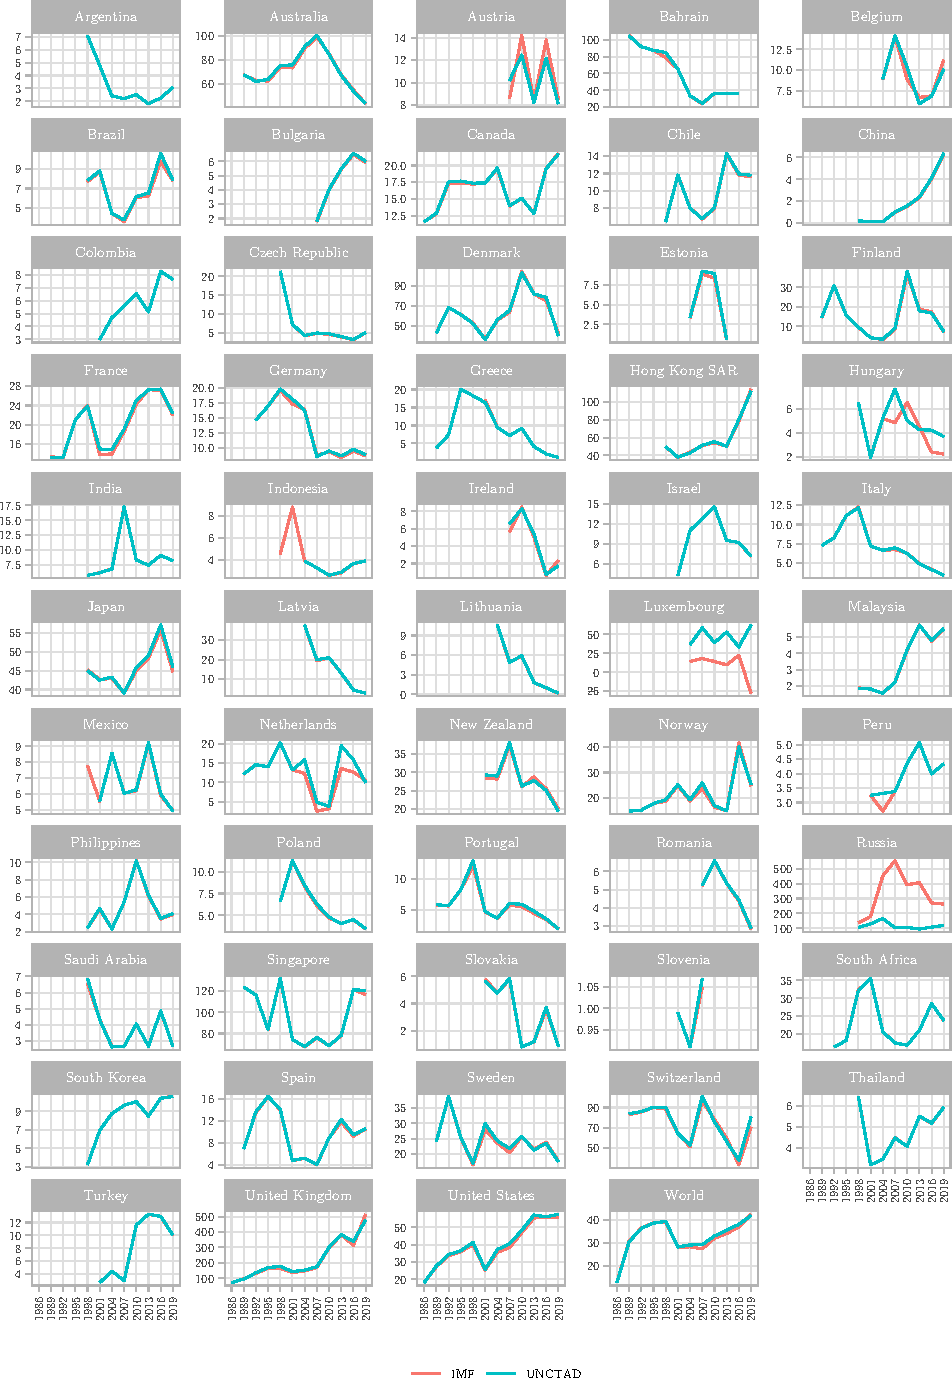
\includegraphics[width=0.99\columnwidth]{_main_files/figure-latex/FigureA11-1} 

}

\caption{Comparison between the FDT ratios calculated using direct investment (DI) data from the IMF and UNCTAD}\label{fig:FigureA11}
\end{figure}

\begin{figure}[!ht]

{\centering 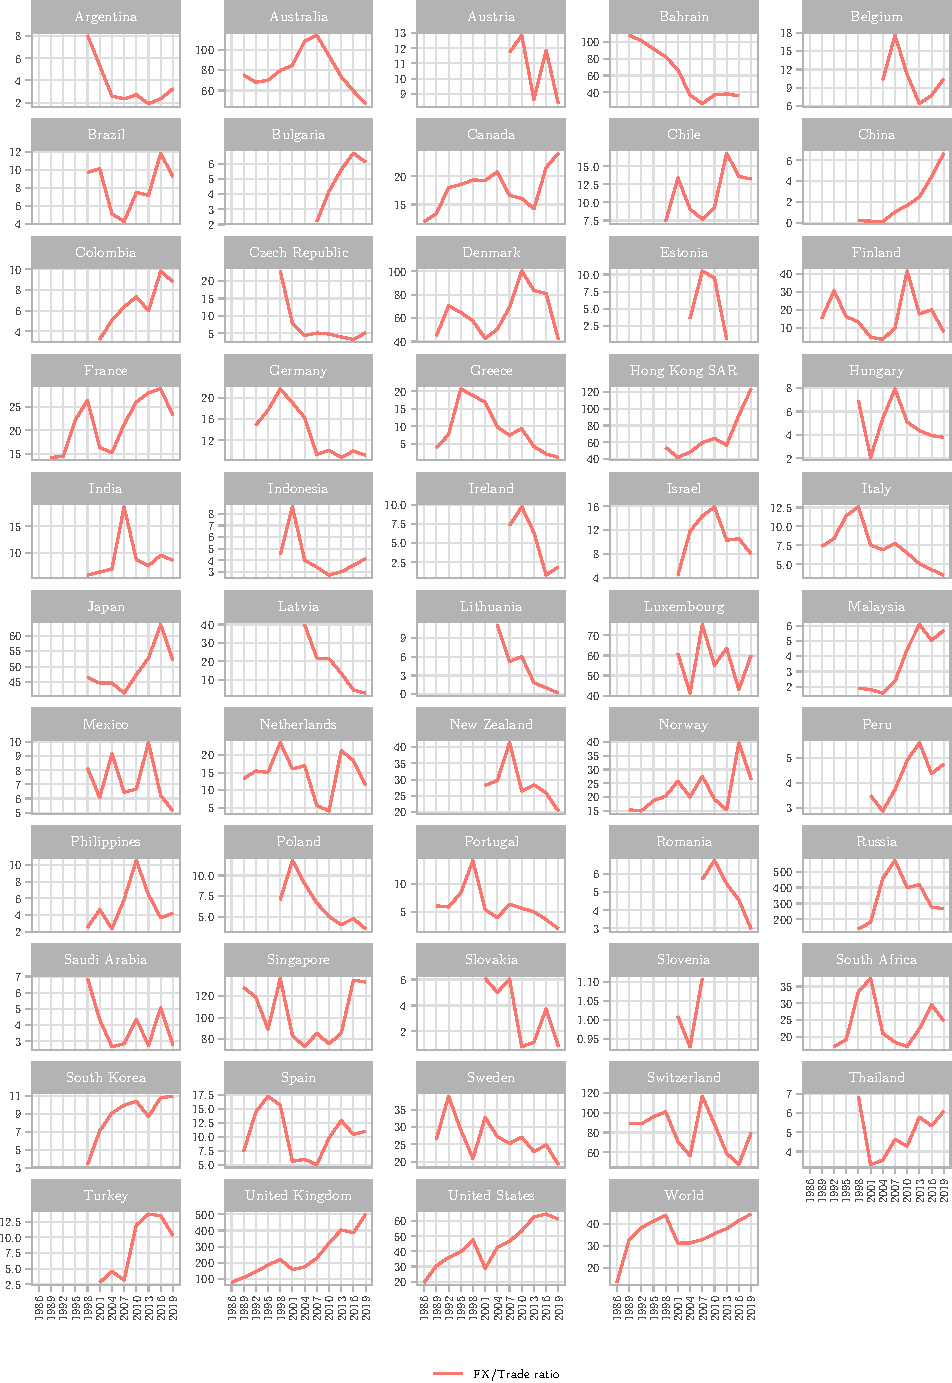
\includegraphics[width=0.99\columnwidth]{_main_files/figure-latex/FigureA12-1} 

}

\caption{FDT ratio calculated using trade data alone}\label{fig:FigureA12}
\end{figure}

\clearpage

\hypertarget{appendixa2}{%
\section{Turnover of OTC foreign exchange instruments, by currency}\label{appendixa2}}

Following the 2019 ranking, Table \ref{tab:TableAA21} shows a very similar list like the one presented in Table \ref{tab:Table22}. The difference is that Taiwan New Dollar could also be upgraded to the list. Regarding the changes from 2016 to 2019, most currencies present stable participation. Contrarily, Chinese Renminbi Yuan, Hong Kong Dollar and Taiwan New Dollar increased significantly their participation\footnote{This could be related to the spillovers of Chinese monetary policy, via the trade channel \autocite{miranda-agrippino2020a}, and to increased renminbi invoicing \autocite{georgiadis2021}.}.




\begin{table}[H]

\caption{\label{tab:TableAA21}Turnover of OTC foreign exchange instruments in billions of US dollars, April 2013-2019 daily averages (``Net-net'' basis)}
\centering
\fontsize{10}{12}\selectfont
\begin{threeparttable}
\begin{tabular}[t]{lrrrrrr}
\toprule
\multicolumn{1}{c}{ } & \multicolumn{2}{c}{2013} & \multicolumn{2}{c}{2016} & \multicolumn{2}{c}{2019} \\
\cmidrule(l{3pt}r{3pt}){2-3} \cmidrule(l{3pt}r{3pt}){4-5} \cmidrule(l{3pt}r{3pt}){6-7}
Currency & Amount & $\%$ & Amount & $\%$ & Amount & $\%$\\
\midrule
US Dollar & 4662 & 87.03 & 4437 & 87.58 & 5824 & 88.31\\
Euro & 1790 & 33.41 & 1590 & 31.39 & 2129 & 32.28\\
Japanese Yen & 1235 & 23.05 & 1096 & 21.63 & 1108 & 16.80\\
Pound Sterling & 633 & 11.82 & 649 & 12.81 & 844 & 12.80\\
Australian Dollar & 463 & 8.64 & 349 & 6.89 & 447 & 6.78\\
Canadian Dollar & 244 & 4.55 & 260 & 5.13 & 332 & 5.03\\
Swiss Franc & 276 & 5.15 & 243 & 4.80 & 327 & 4.96\\
Chinese Yuan (Renminbi) & 120 & 2.24 & 202 & 3.99 & 285 & 4.32\\
Hong Kong Dollar & 77 & 1.44 & 88 & 1.74 & 233 & 3.53\\
New Zealand Dollar & 105 & 1.96 & 104 & 2.05 & 137 & 2.08\\
Swedish Krona & 94 & 1.75 & 112 & 2.21 & 134 & 2.03\\
South Korean Won & 64 & 1.19 & 84 & 1.66 & 132 & 2.00\\
Norwegian Krone & 77 & 1.44 & 85 & 1.68 & 119 & 1.80\\
Singapore Dollar & 75 & 1.40 & 91 & 1.80 & 119 & 1.80\\
Indian Rupee & 53 & 0.99 & 58 & 1.14 & 114 & 1.73\\
Mexican Peso & 135 & 2.52 & 97 & 1.91 & 114 & 1.73\\
Russian Rouble & 86 & 1.61 & 58 & 1.14 & 72 & 1.09\\
South African Rand & 60 & 1.12 & 49 & 0.97 & 72 & 1.09\\
Brazilian Real & 59 & 1.10 & 51 & 1.01 & 71 & 1.08\\
Turkish New Lira & 71 & 1.33 & 73 & 1.44 & 71 & 1.08\\
Taiwan New Dollar & 24 & 0.45 & 32 & 0.63 & 60 & 0.91\\
Danish Krone & 42 & 0.78 & 42 & 0.83 & 42 & 0.64\\
Poland New Zloty & 38 & 0.71 & 35 & 0.69 & 41 & 0.62\\
Thai Baht & 17 & 0.32 & 18 & 0.36 & 32 & 0.49\\
Hungarian Forint & 23 & 0.43 & 15 & 0.30 & 27 & 0.41\\
\midrule
Total (all currencies) & 5357 & 200.00 & 5066 & 200.00 & 6595 & 200.00\\
\bottomrule
\end{tabular}
\begin{tablenotes}[para]
\item \textit{\footnotesize{Source:}} 
\item \footnotesize{Adapted from \textcite{bankforinternationalsettlements2021b}. ``As two currencies are involved in each transaction, the sum of shares in individual currencies will total 200\%.'' \autocite[\text{p.} 5]{bankforinternationalsettlements2019}}
\end{tablenotes}
\end{threeparttable}
\end{table}

\clearpage

\hypertarget{appendixa3}{%
\section{Reportable futures and options positions for other currencies}\label{appendixa3}}

\begin{figure}[!ht]

{\centering 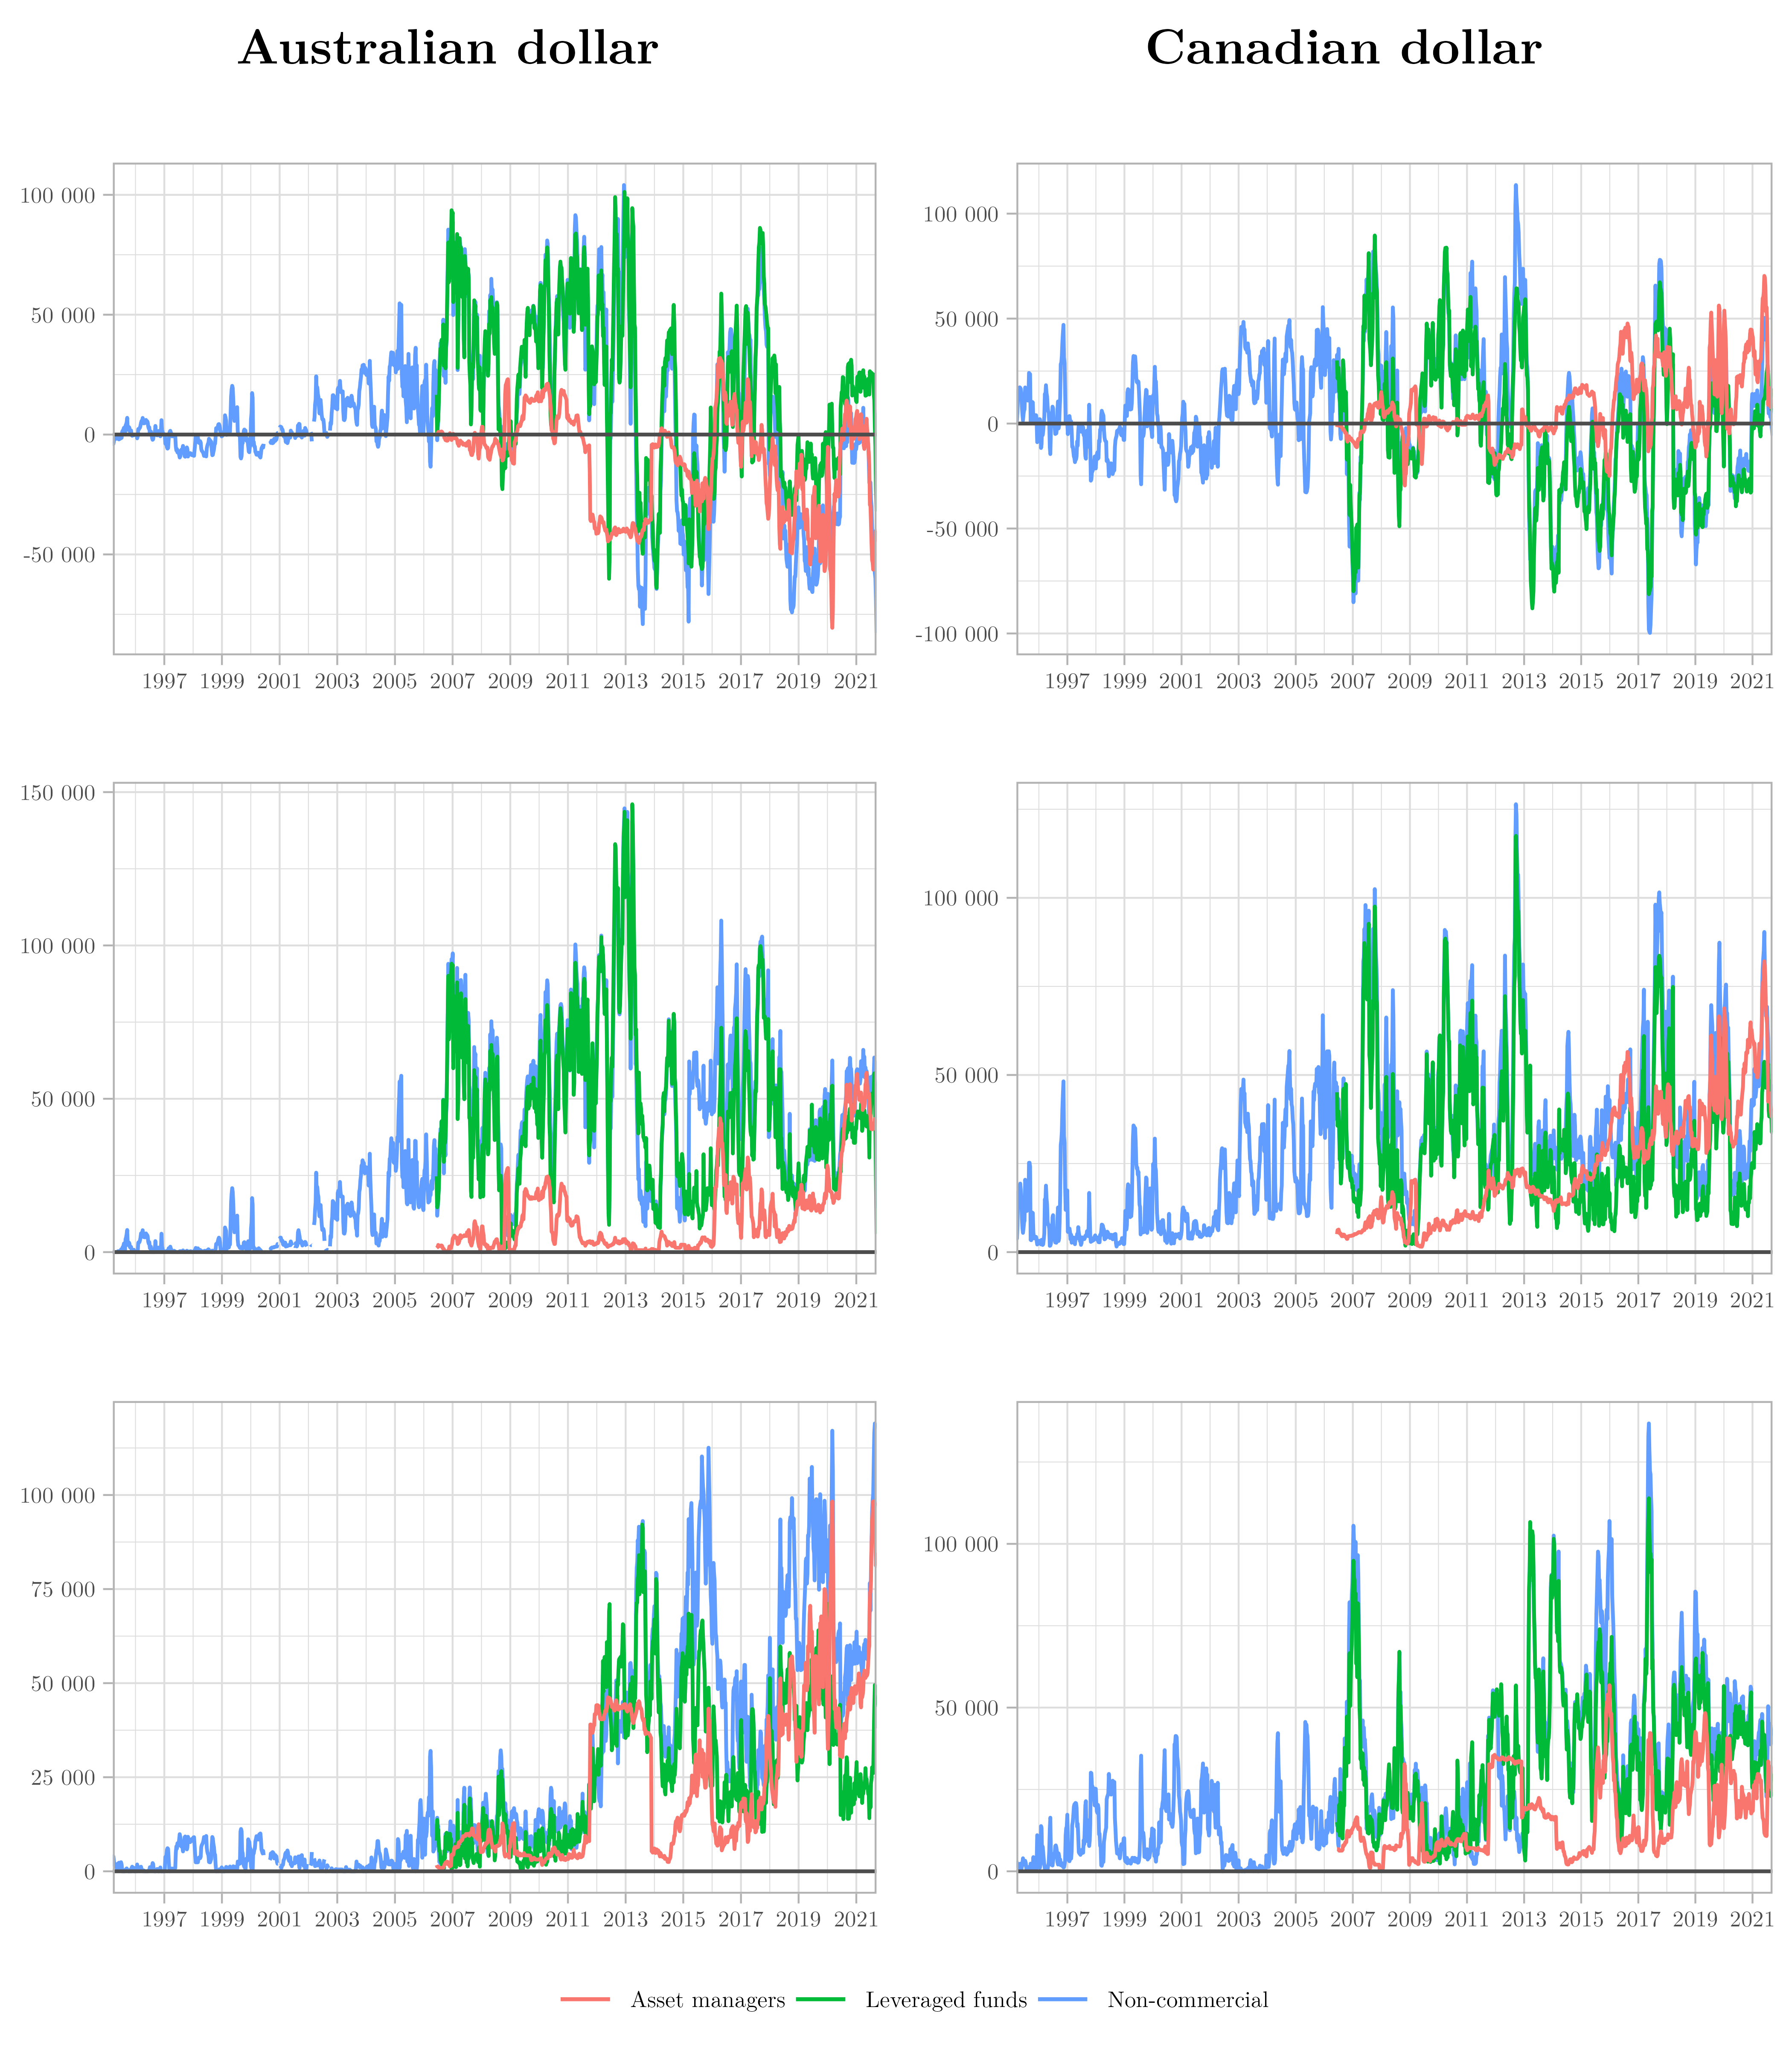
\includegraphics[width=0.99\columnwidth]{figure/GTOG_AUDCAD} 

}

\caption[Reportable futures and options positions on the Chicago Mercantile Exchange for Australian dollar and Canadian dollar, in number of contracts, 1995-03-21 to 2021-09-14]{Reportable futures and options positions on the Chicago Mercantile Exchange for Australian dollar and Canadian dollar, in number of contracts, 1995-03-21 to 2021-09-14 \\ \scriptsize \textit{Source:} Commodity Futures Trading Commission (CFTC). \\ \scriptsize \textit{Notes:} Regarding the contract size, the values are AUD 100 000 and CAD 100 000, respectively.}\label{fig:FigureA31}
\end{figure}

\clearpage

\begin{figure}[!ht]

{\centering 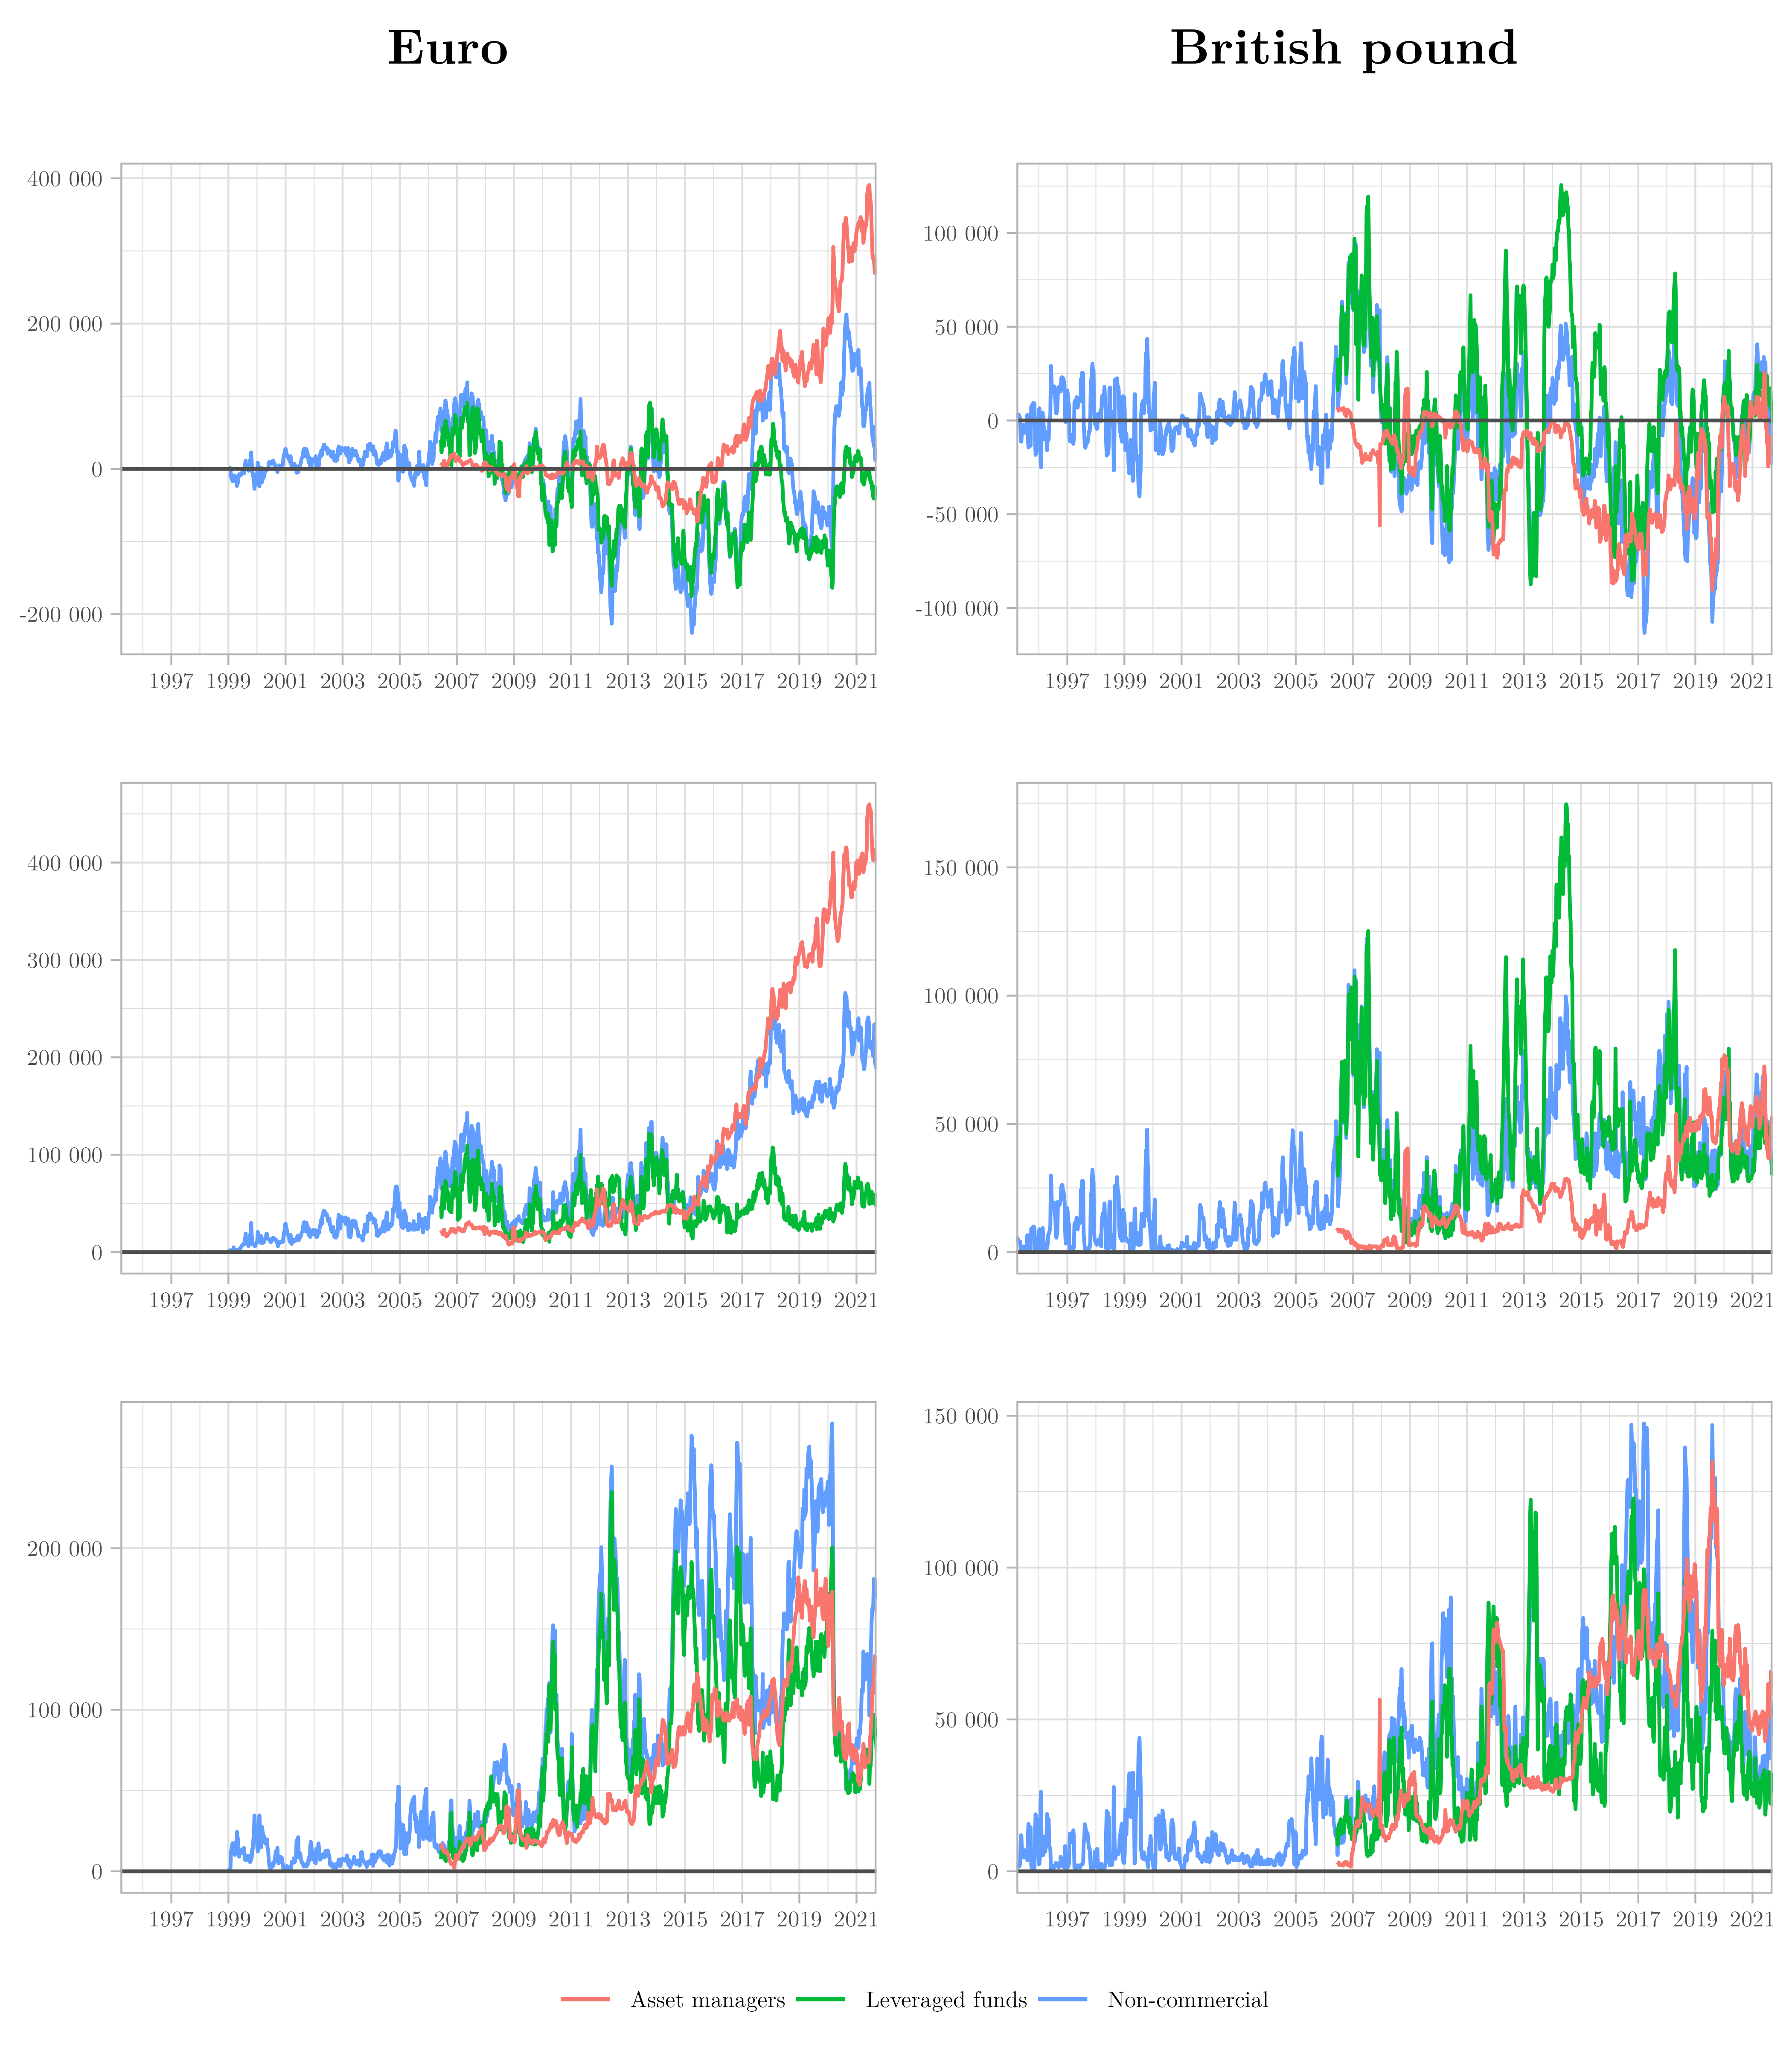
\includegraphics[width=0.99\columnwidth]{figure/GTOG_EURGBP} 

}

\caption[Reportable futures and options positions on the Chicago Mercantile Exchange for euro and British pound, in number of contracts, 1995-03-21 to 2021-09-14]{Reportable futures and options positions on the Chicago Mercantile Exchange for euro and British pound, in number of contracts, 1995-03-21 to 2021-09-14 \\ \scriptsize \textit{Source:} Commodity Futures Trading Commission (CFTC). \\ \scriptsize \textit{Notes:} Regarding the contract size, the values are EUR 125 000 and GBP 62 500, respectively.}\label{fig:FigureA32}
\end{figure}

\clearpage

\begin{figure}[!ht]

{\centering 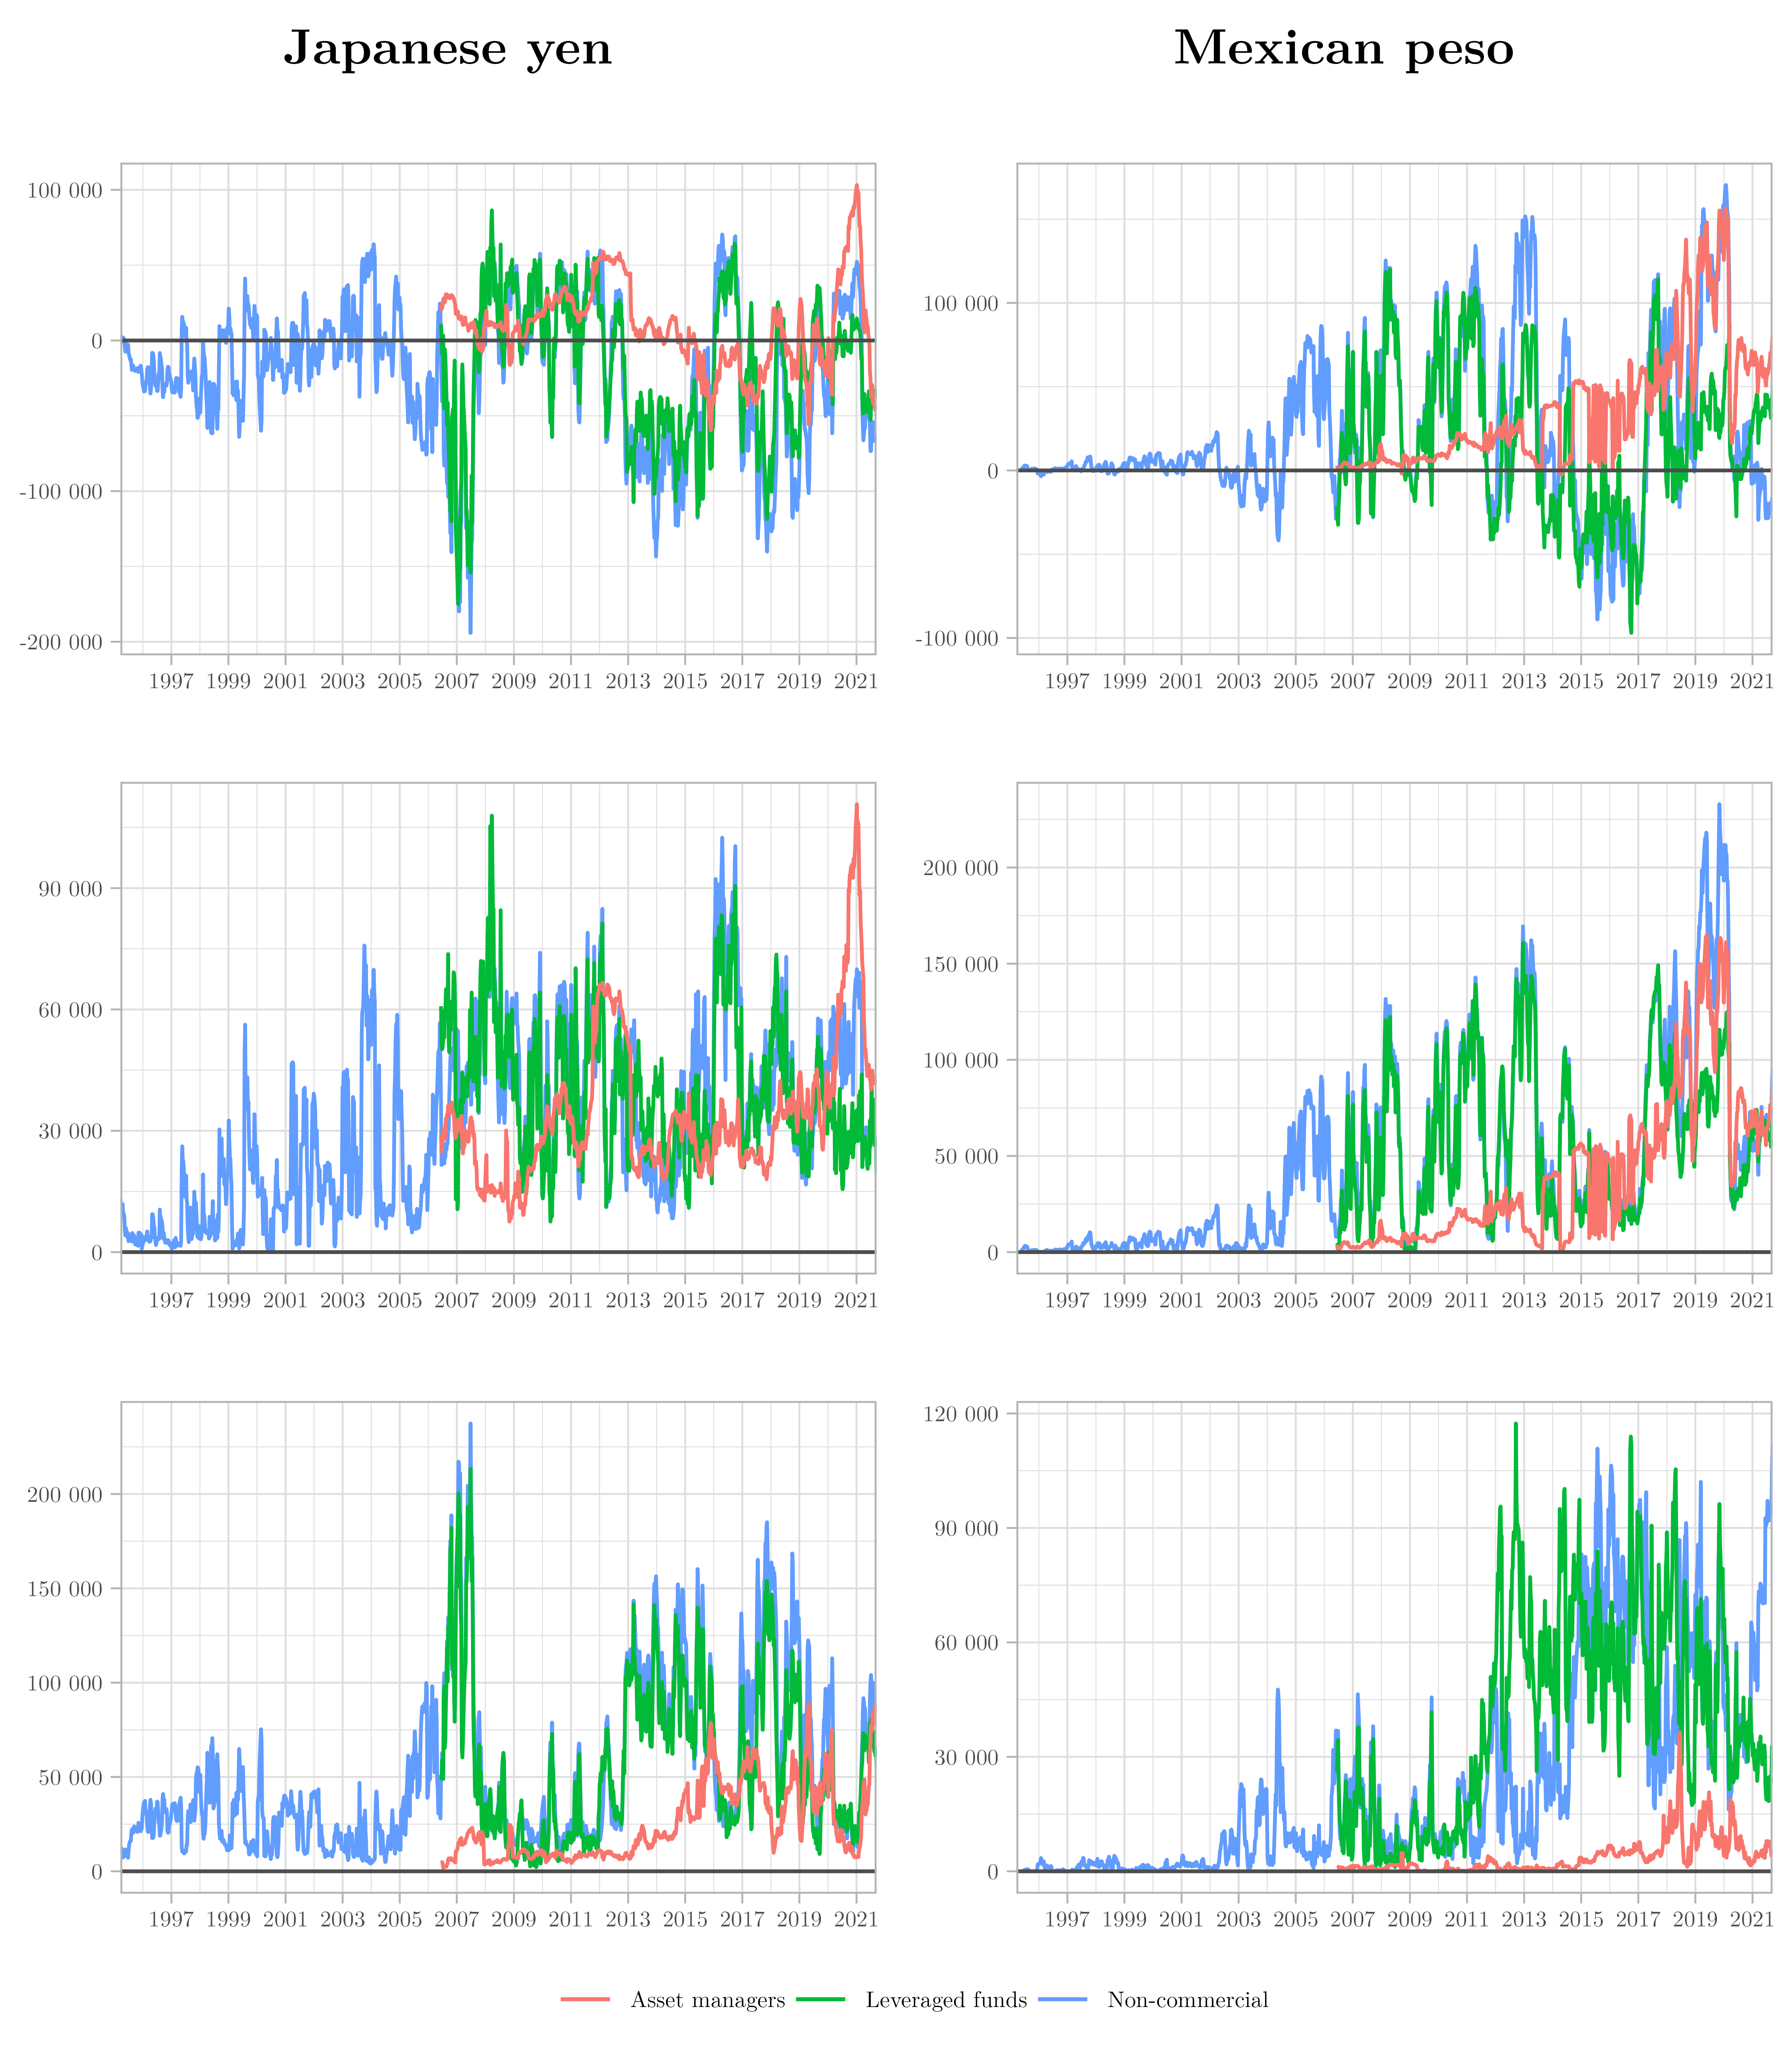
\includegraphics[width=0.99\columnwidth]{figure/GTOG_JPYMXN} 

}

\caption[Reportable futures and options positions on the Chicago Mercantile Exchange for Japanese yen and Mexican peso, in number of contracts, 1995-03-21 to 2021-09-14]{Reportable futures and options positions on the Chicago Mercantile Exchange for Japanese yen and Mexican peso, in number of contracts, 1995-03-21 to 2021-09-14 \\ \scriptsize \textit{Source:} Commodity Futures Trading Commission (CFTC). \\ \scriptsize \textit{Notes:} Regarding the contract size, the values are JPY 12 500 000 and MXN 500 000, respectively.}\label{fig:FigureA33}
\end{figure}

\clearpage

\begin{figure}[!ht]

{\centering 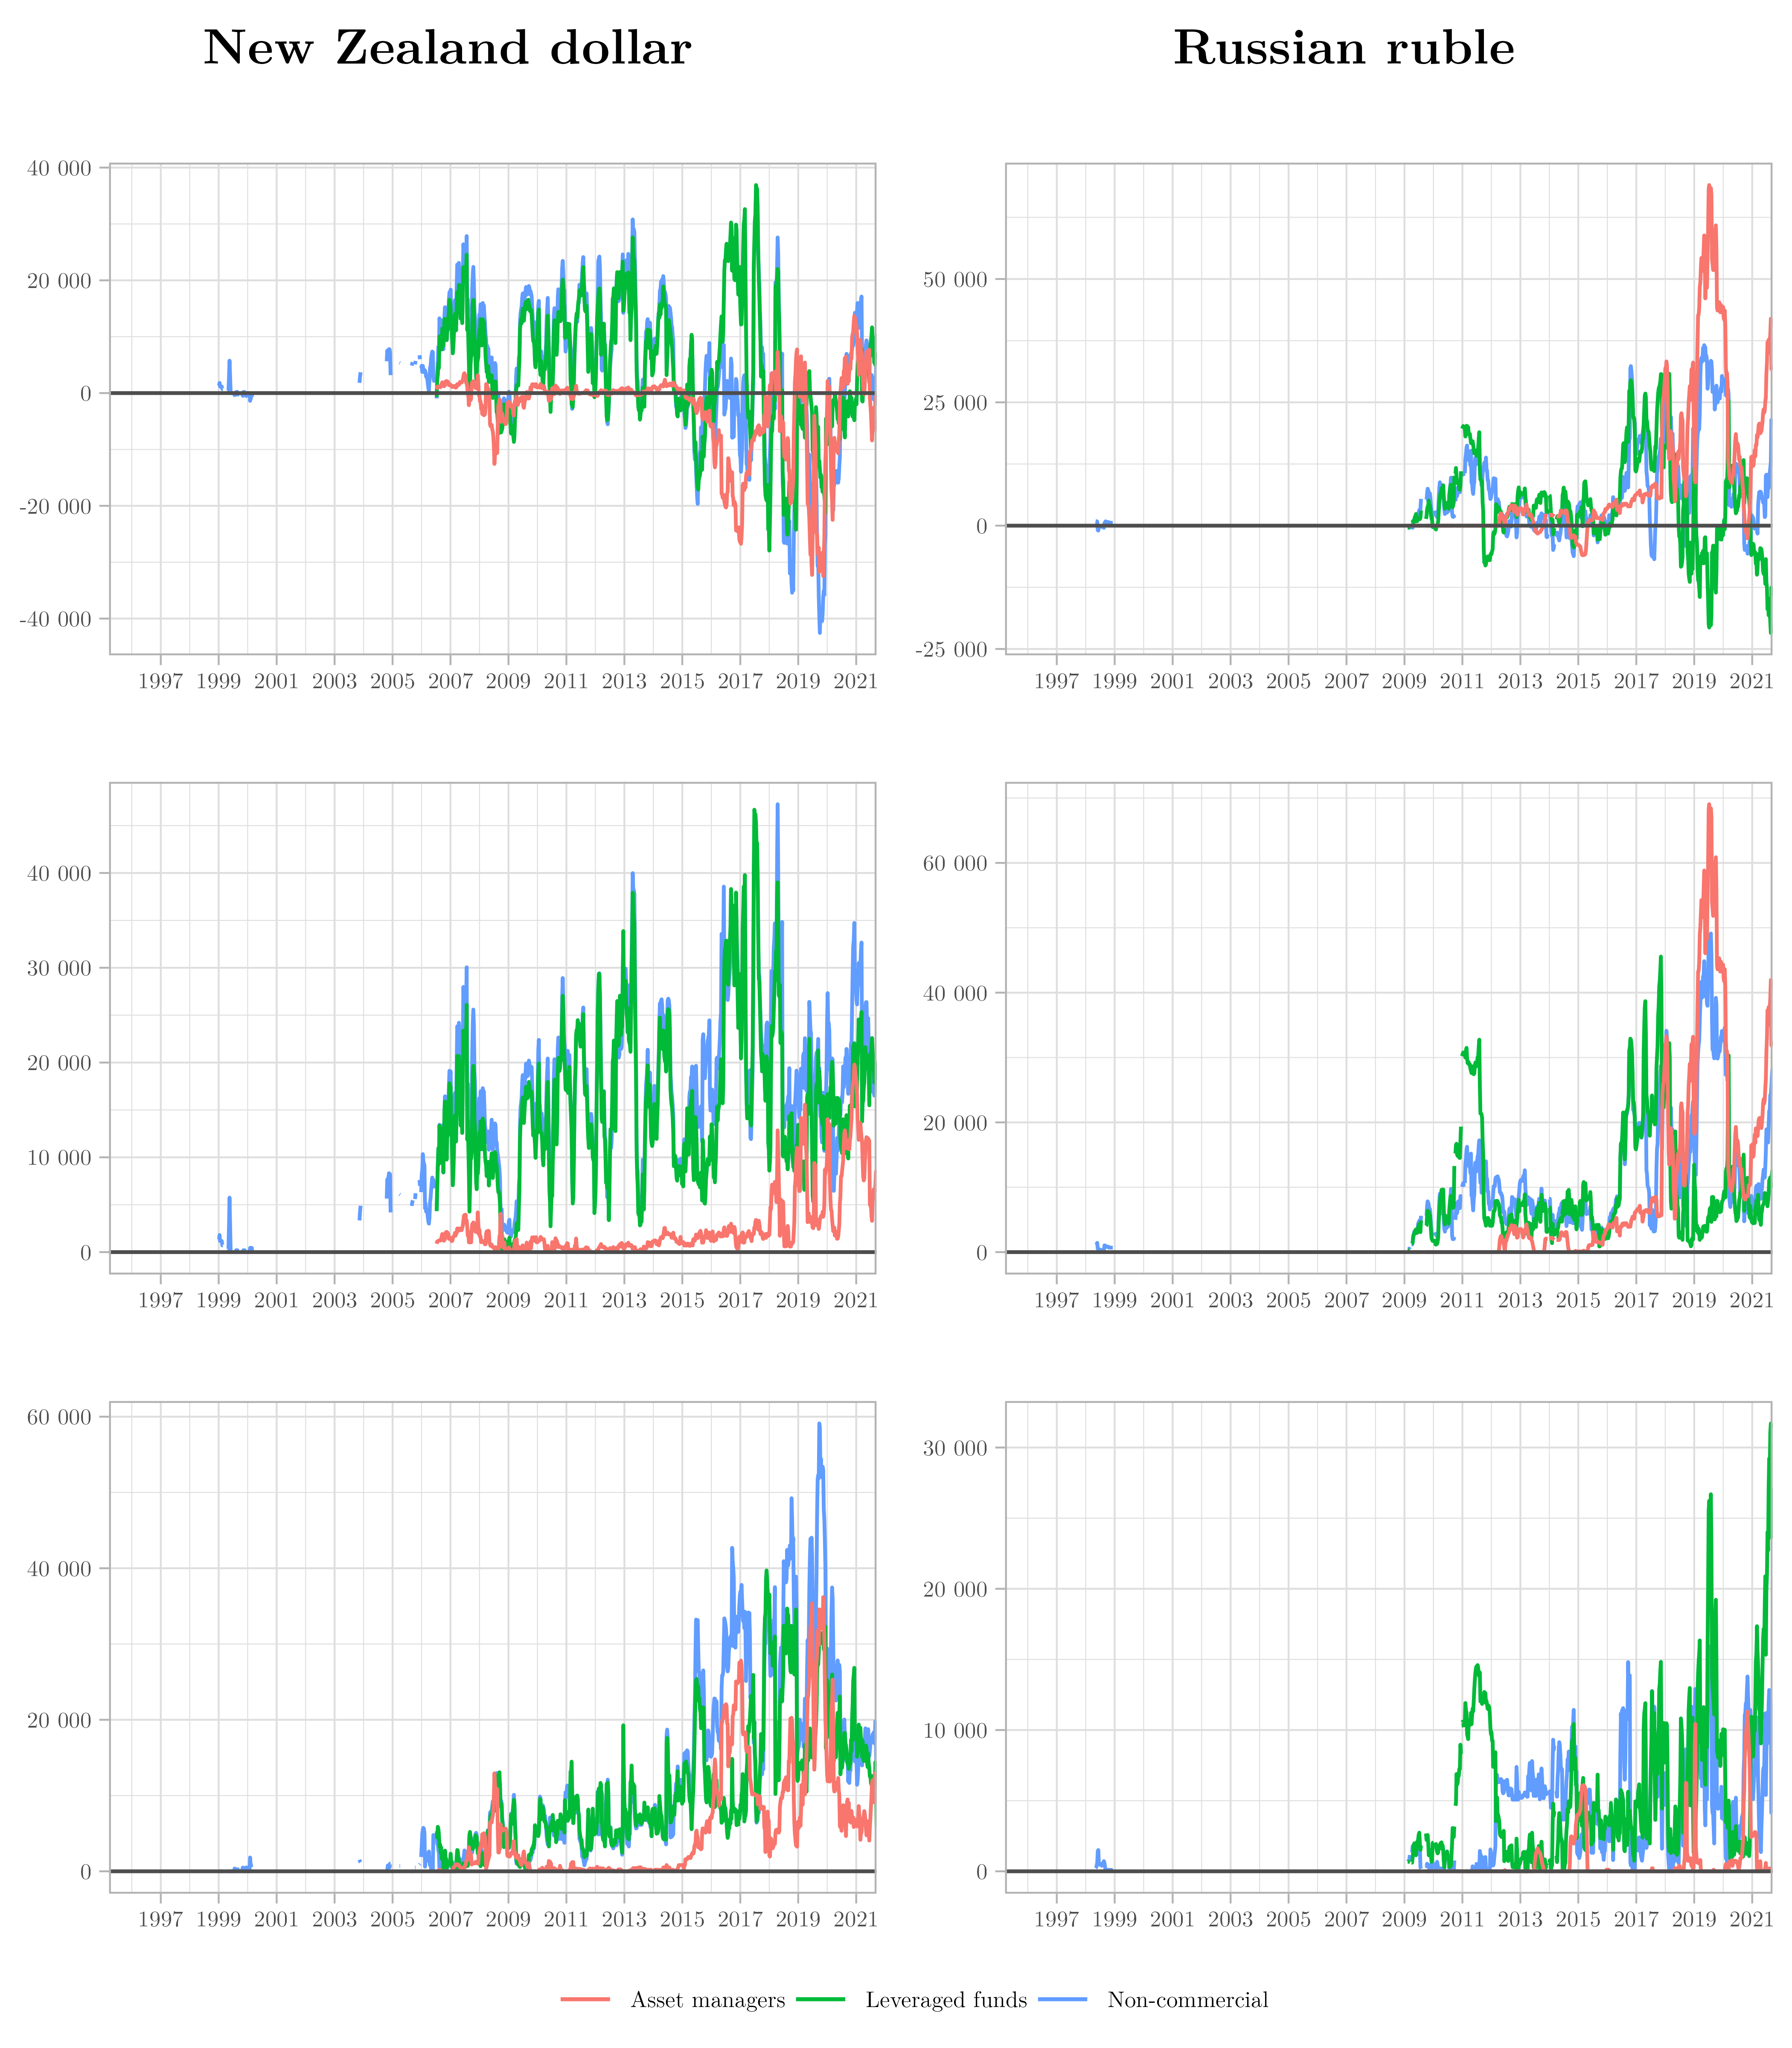
\includegraphics[width=0.99\columnwidth]{figure/GTOG_NZDRBL} 

}

\caption[Reportable futures and options positions on the Chicago Mercantile Exchange for New Zealand dollar and Russian ruble, in number of contracts, 1995-03-21 to 2021-09-14]{Reportable futures and options positions on the Chicago Mercantile Exchange for New Zealand dollar and Russian ruble, in number of contracts, 1995-03-21 to 2021-09-14 \\ \scriptsize \textit{Source:} Commodity Futures Trading Commission (CFTC). \\ \scriptsize \textit{Notes:} Regarding the contract size, the values are NZD 100 000 and RBL 2 500 000, respectively.}\label{fig:FigureA34}
\end{figure}

\clearpage

\begin{figure}[!ht]

{\centering 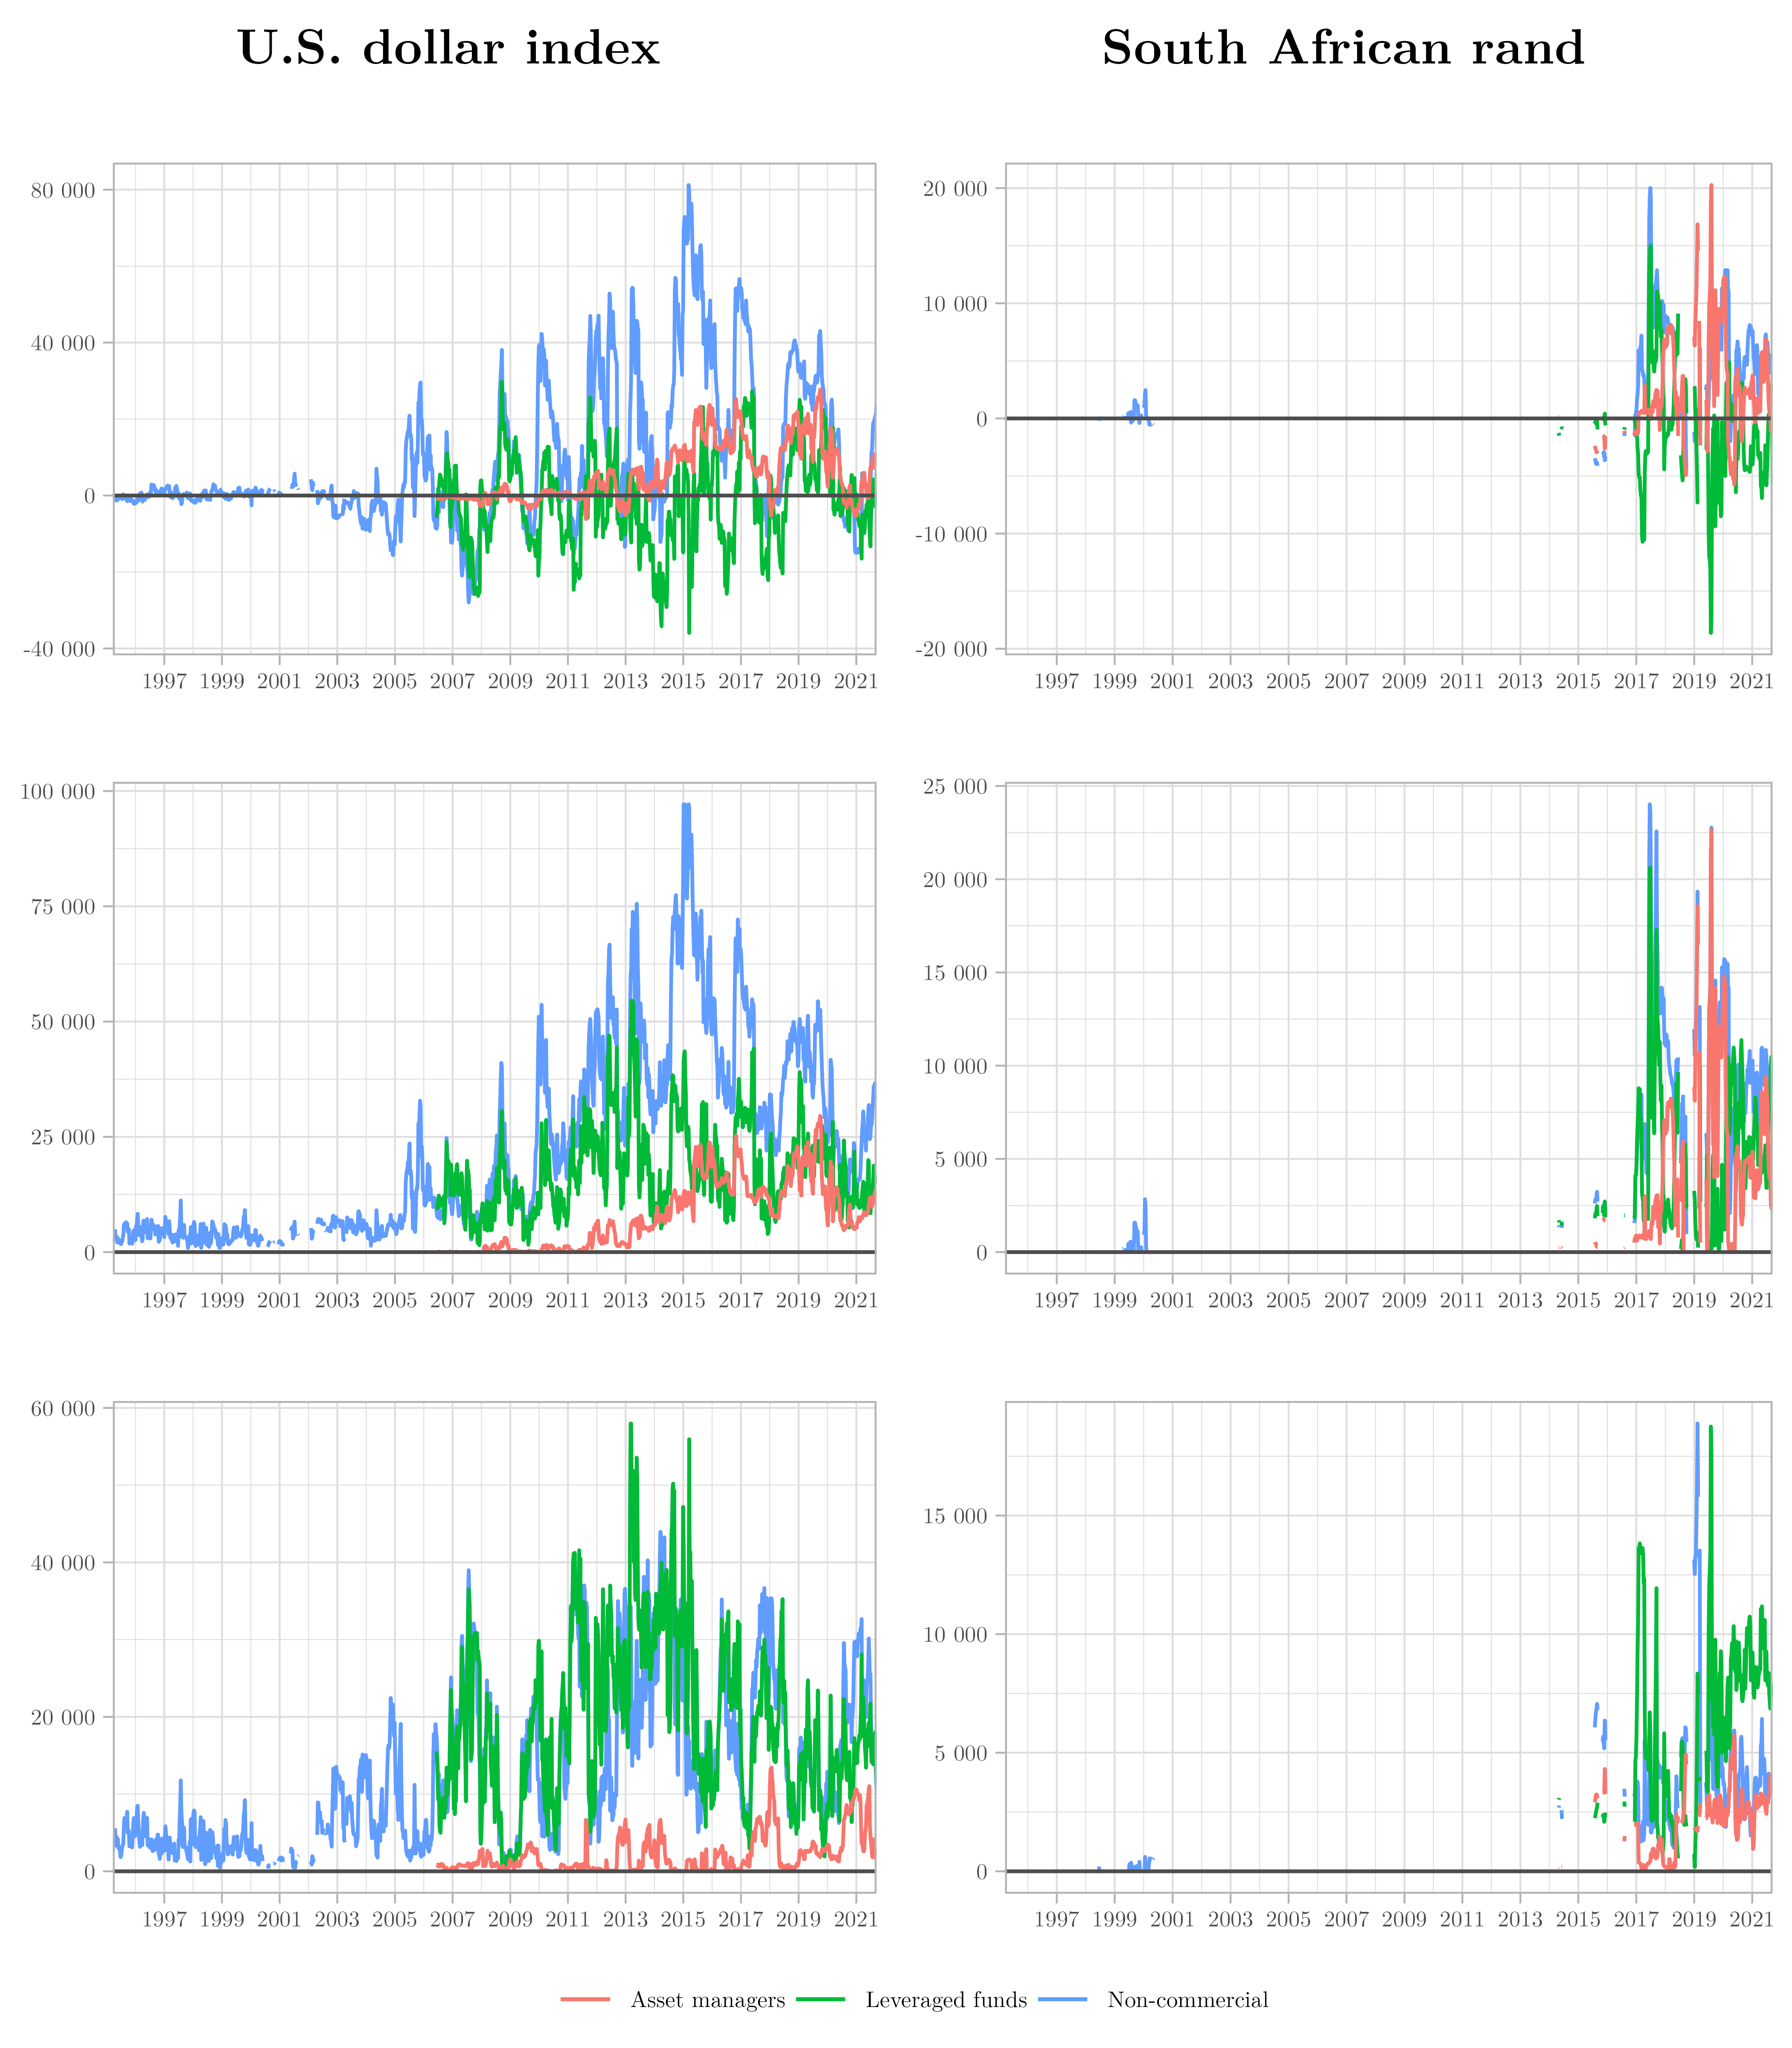
\includegraphics[width=0.99\columnwidth]{figure/GTOG_USDZAR} 

}

\caption[Reportable futures and options positions on the Chicago Mercantile Exchange for U.S. dollar index and South African rand, in number of contracts, 1995-03-21 to 2021-09-14]{Reportable futures and options positions on the Chicago Mercantile Exchange for U.S. dollar index and South African rand, in number of contracts, 1995-03-21 to 2021-09-14 \\ \scriptsize \textit{Source:} Commodity Futures Trading Commission (CFTC). \\ \scriptsize \textit{Notes:} Regarding the contract size, the values are USD 1 000 and ZAR 2 500 000, respectively.}\label{fig:FigureA35}
\end{figure}

\clearpage

\hypertarget{appendixa4}{%
\section{Sentiment index}\label{appendixa4}}

The sentiment index is formulated by Wang \autocite*{wang2001,wang2004}. The main advantages of the investor-sentiment index are related to its: (i) usual measure for sentiment in other market instruments, being widely accepted by futures traders, (ii) intuitive way to follow trader actions, and (iii) way to compare ``return predictability across futures markets, while raw positions make the comparisons impossible due to the diverse structure across futures markets.'' \autocite[\text{p.} 933]{wang2001} As elaborated by practitioners \autocite{freecotdata2021}, the sentiment index (\(SI\)) with net positions as a share of total positions (\(S\)) is given by
\begin{equation}
SI_{it}^{j} = \frac{S_{it}^{j}-\min{S_{it}^{j}}}{\max{S_{it}^{j}}-\min{S_{it}^{j}}}
\label{eq:17}
\end{equation}

\noindent where \(j\) is the market, \(i\) is the trader type, \(t\) is the period and ``\(\min{S_{it}^{j}}\) and \(\max{S_{it}^{j}}\) represent historical maximum and minimum {[}\ldots{]} over the previous three years.'' \autocite[\text{p.} 933]{wang2001} Figure \ref{fig:Figure29} displays the results for Swiss franc and Brazilian real, with other currencies displayed in Figures \ref{fig:FigureA36} and \ref{fig:FigureA37}. For example, when 100\% is reached for speculators, it means they are more net long than they had ever been in the past three years (three-year percentile).

\begin{figure}[!ht]

{\centering 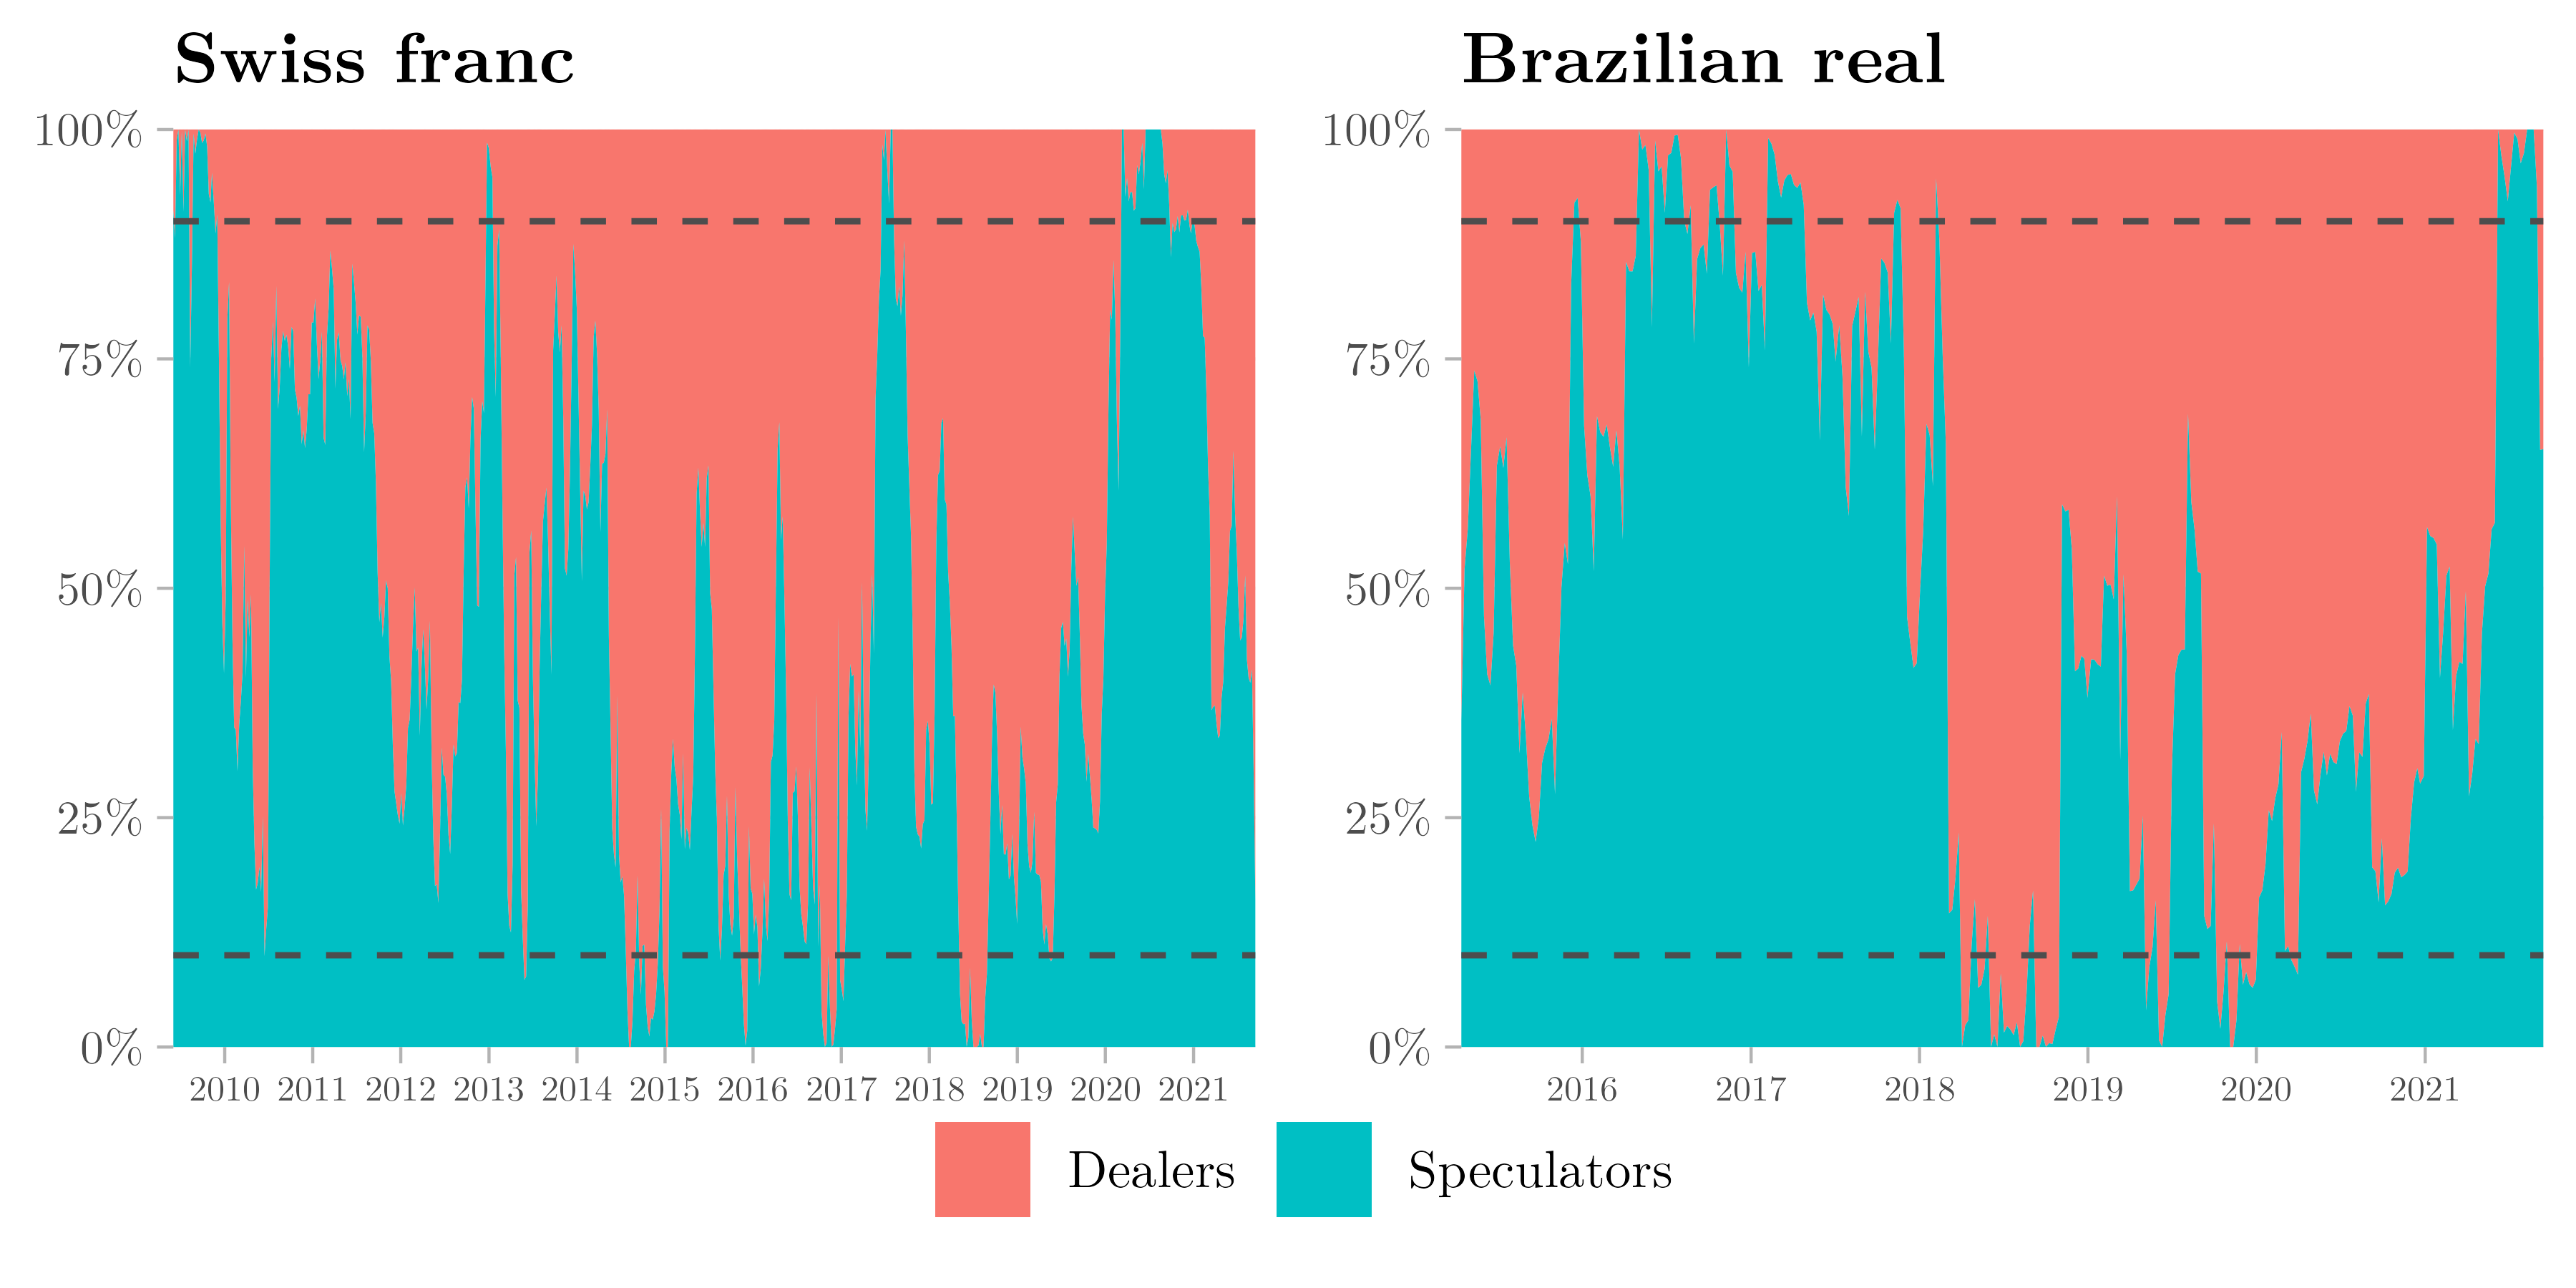
\includegraphics[width=0.80\columnwidth]{figure/CHFBRL} 

}

\caption[Sentiment index for Swiss franc (2009-06-02 to 2021-09-21) and Brazilian real (2015-04-14 to 2021-09-21), three-year percentile]{Sentiment index for Swiss franc (2009-06-02 to 2021-09-21) and Brazilian real (2015-04-14 to 2021-09-21), three-year percentile \\ \scriptsize \textit{Source:} Commodity Futures Trading Commission (CFTC). \\ \scriptsize \textit{Notes:} Speculators are composed by asset managers, leveraged funds, other reportable positions, and non reportable positions. Dashed lines represent the extreme positions (10\% and 90\%).}\label{fig:Figure29}
\end{figure}

\clearpage

\begin{figure}[!ht]

{\centering 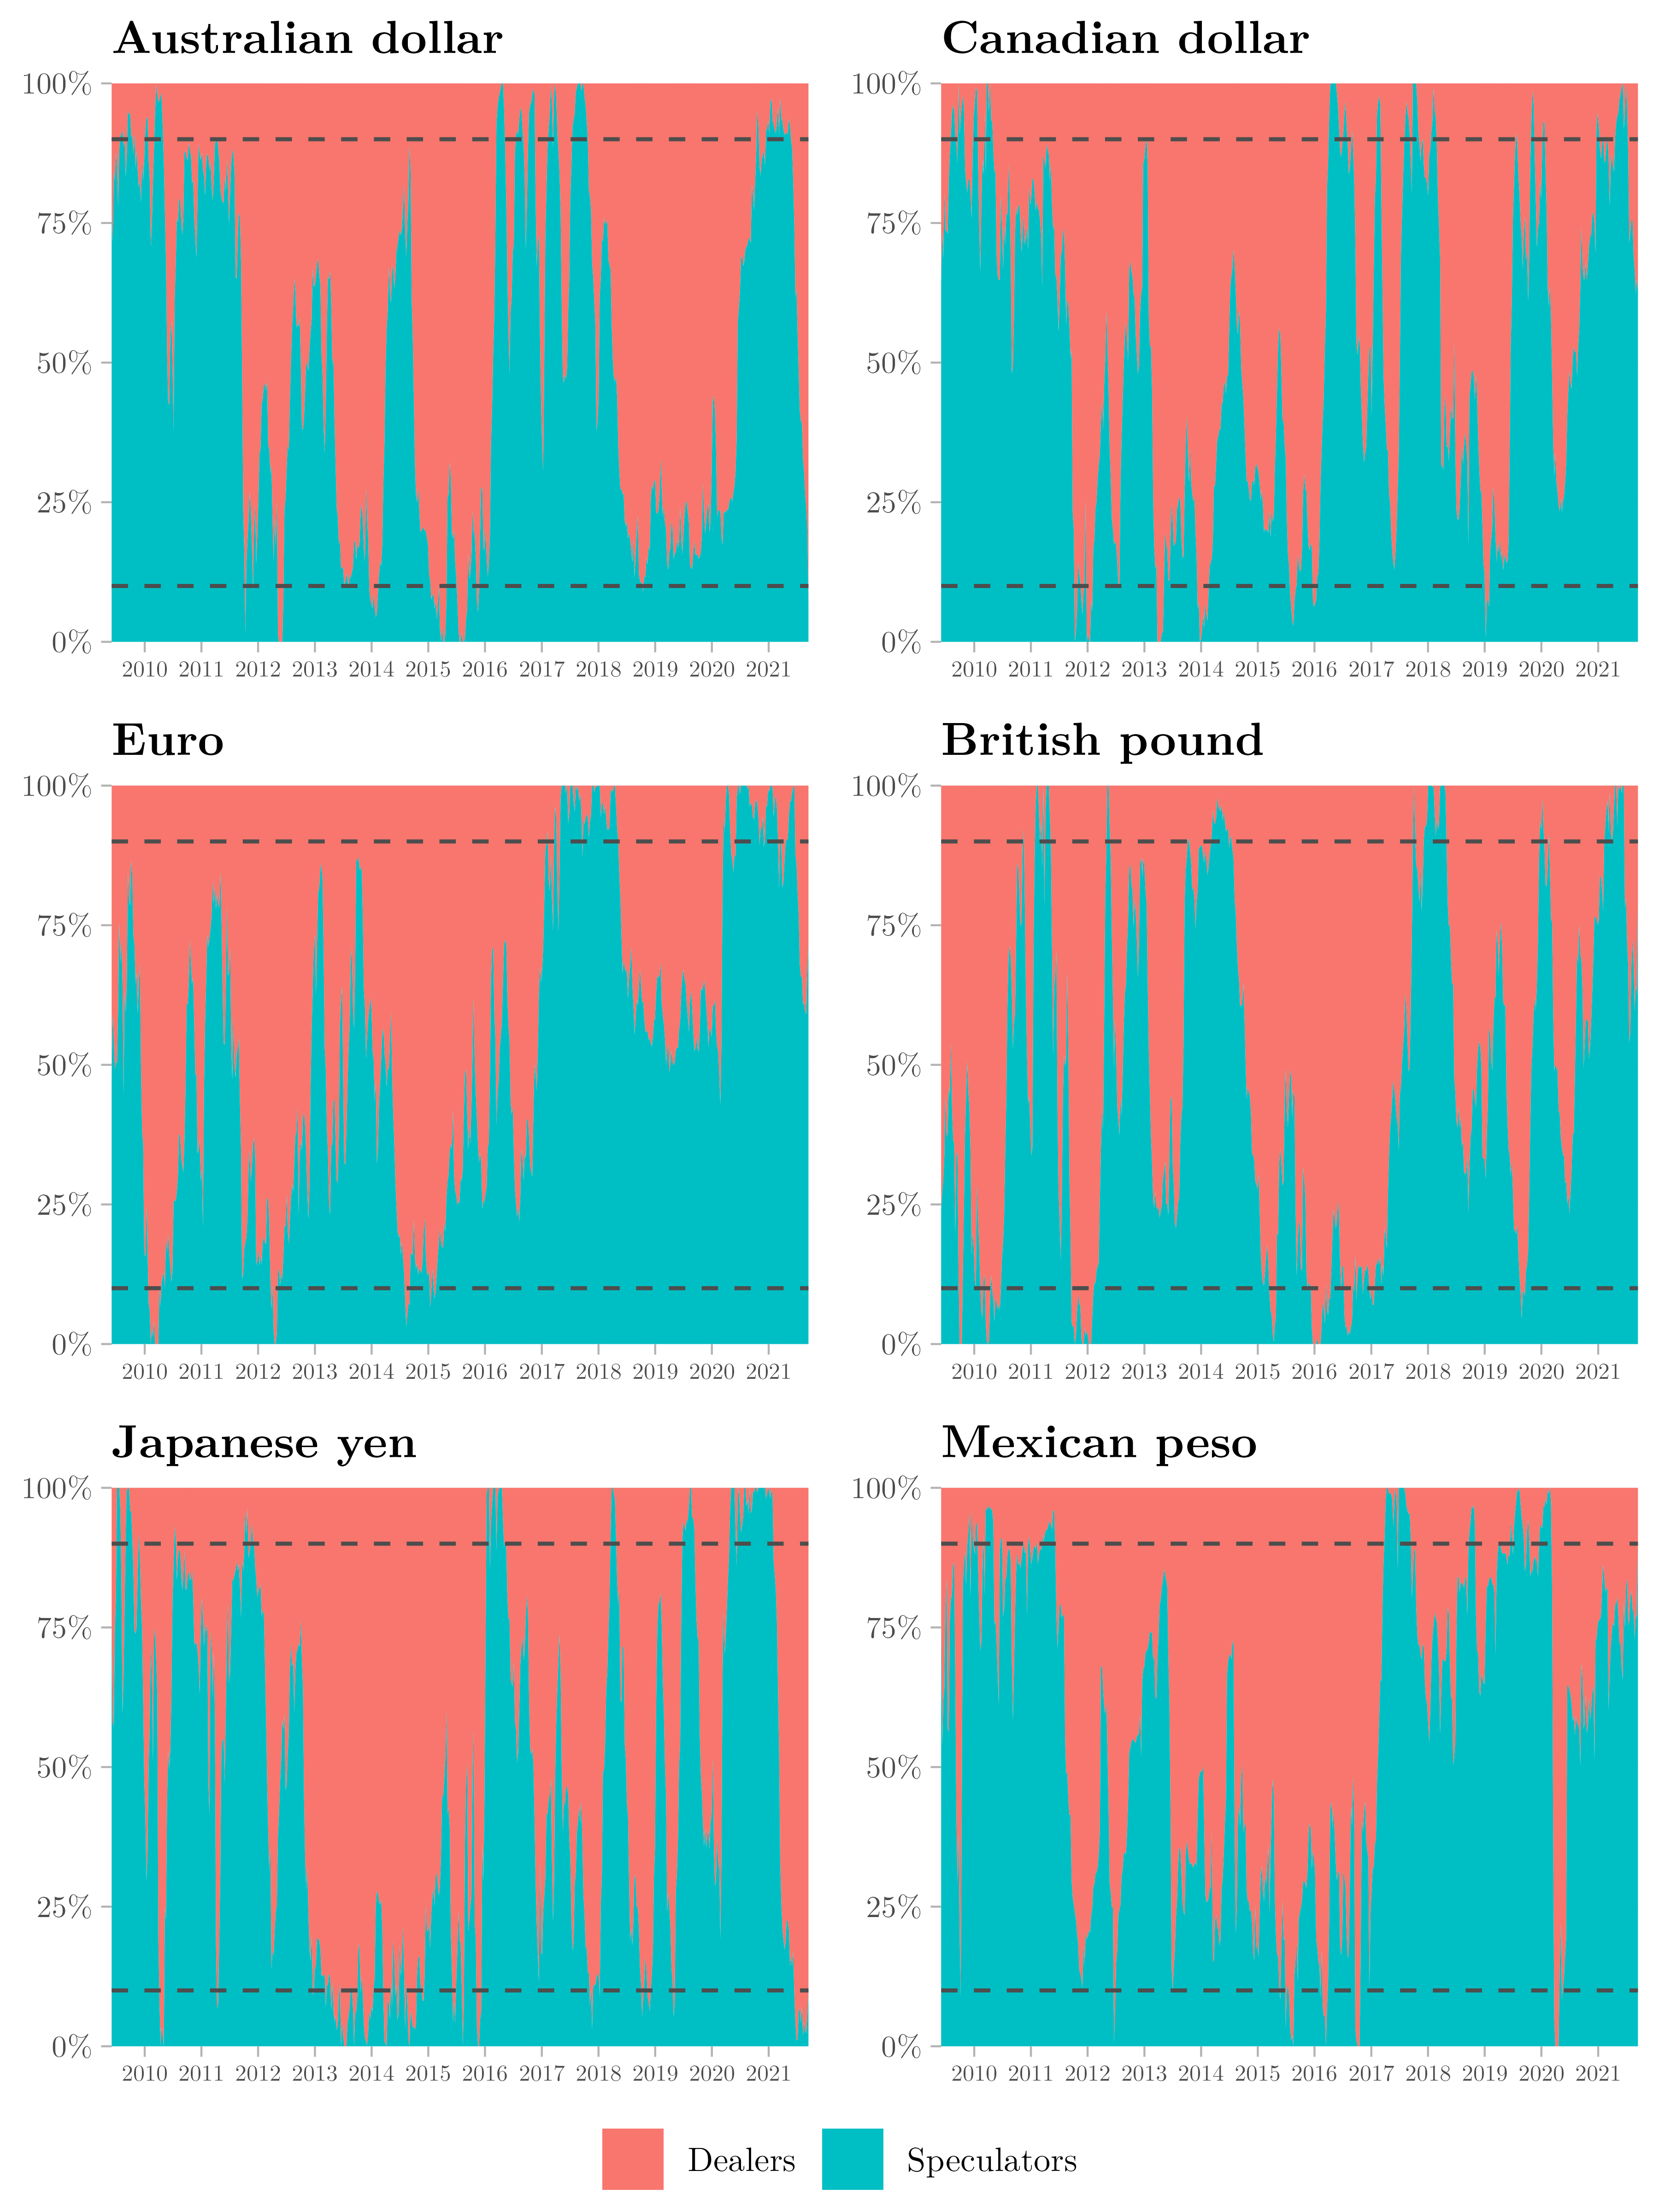
\includegraphics[width=0.99\columnwidth]{figure/OTHERCUR_1} 

}

\caption[Sentiment index for Australian dollar, Canadian dollar, euro, British pound, Japanese yen and Mexican peso, three-year percentile, 2009-06-02 to 2021-09-21]{Sentiment index for Australian dollar, Canadian dollar, euro, British pound, Japanese yen and Mexican peso, three-year percentile, 2009-06-02 to 2021-09-21 \\ \scriptsize \textit{Source:} Commodity Futures Trading Commission (CFTC).}\label{fig:FigureA36}
\end{figure}

\clearpage

\begin{figure}[!ht]

{\centering 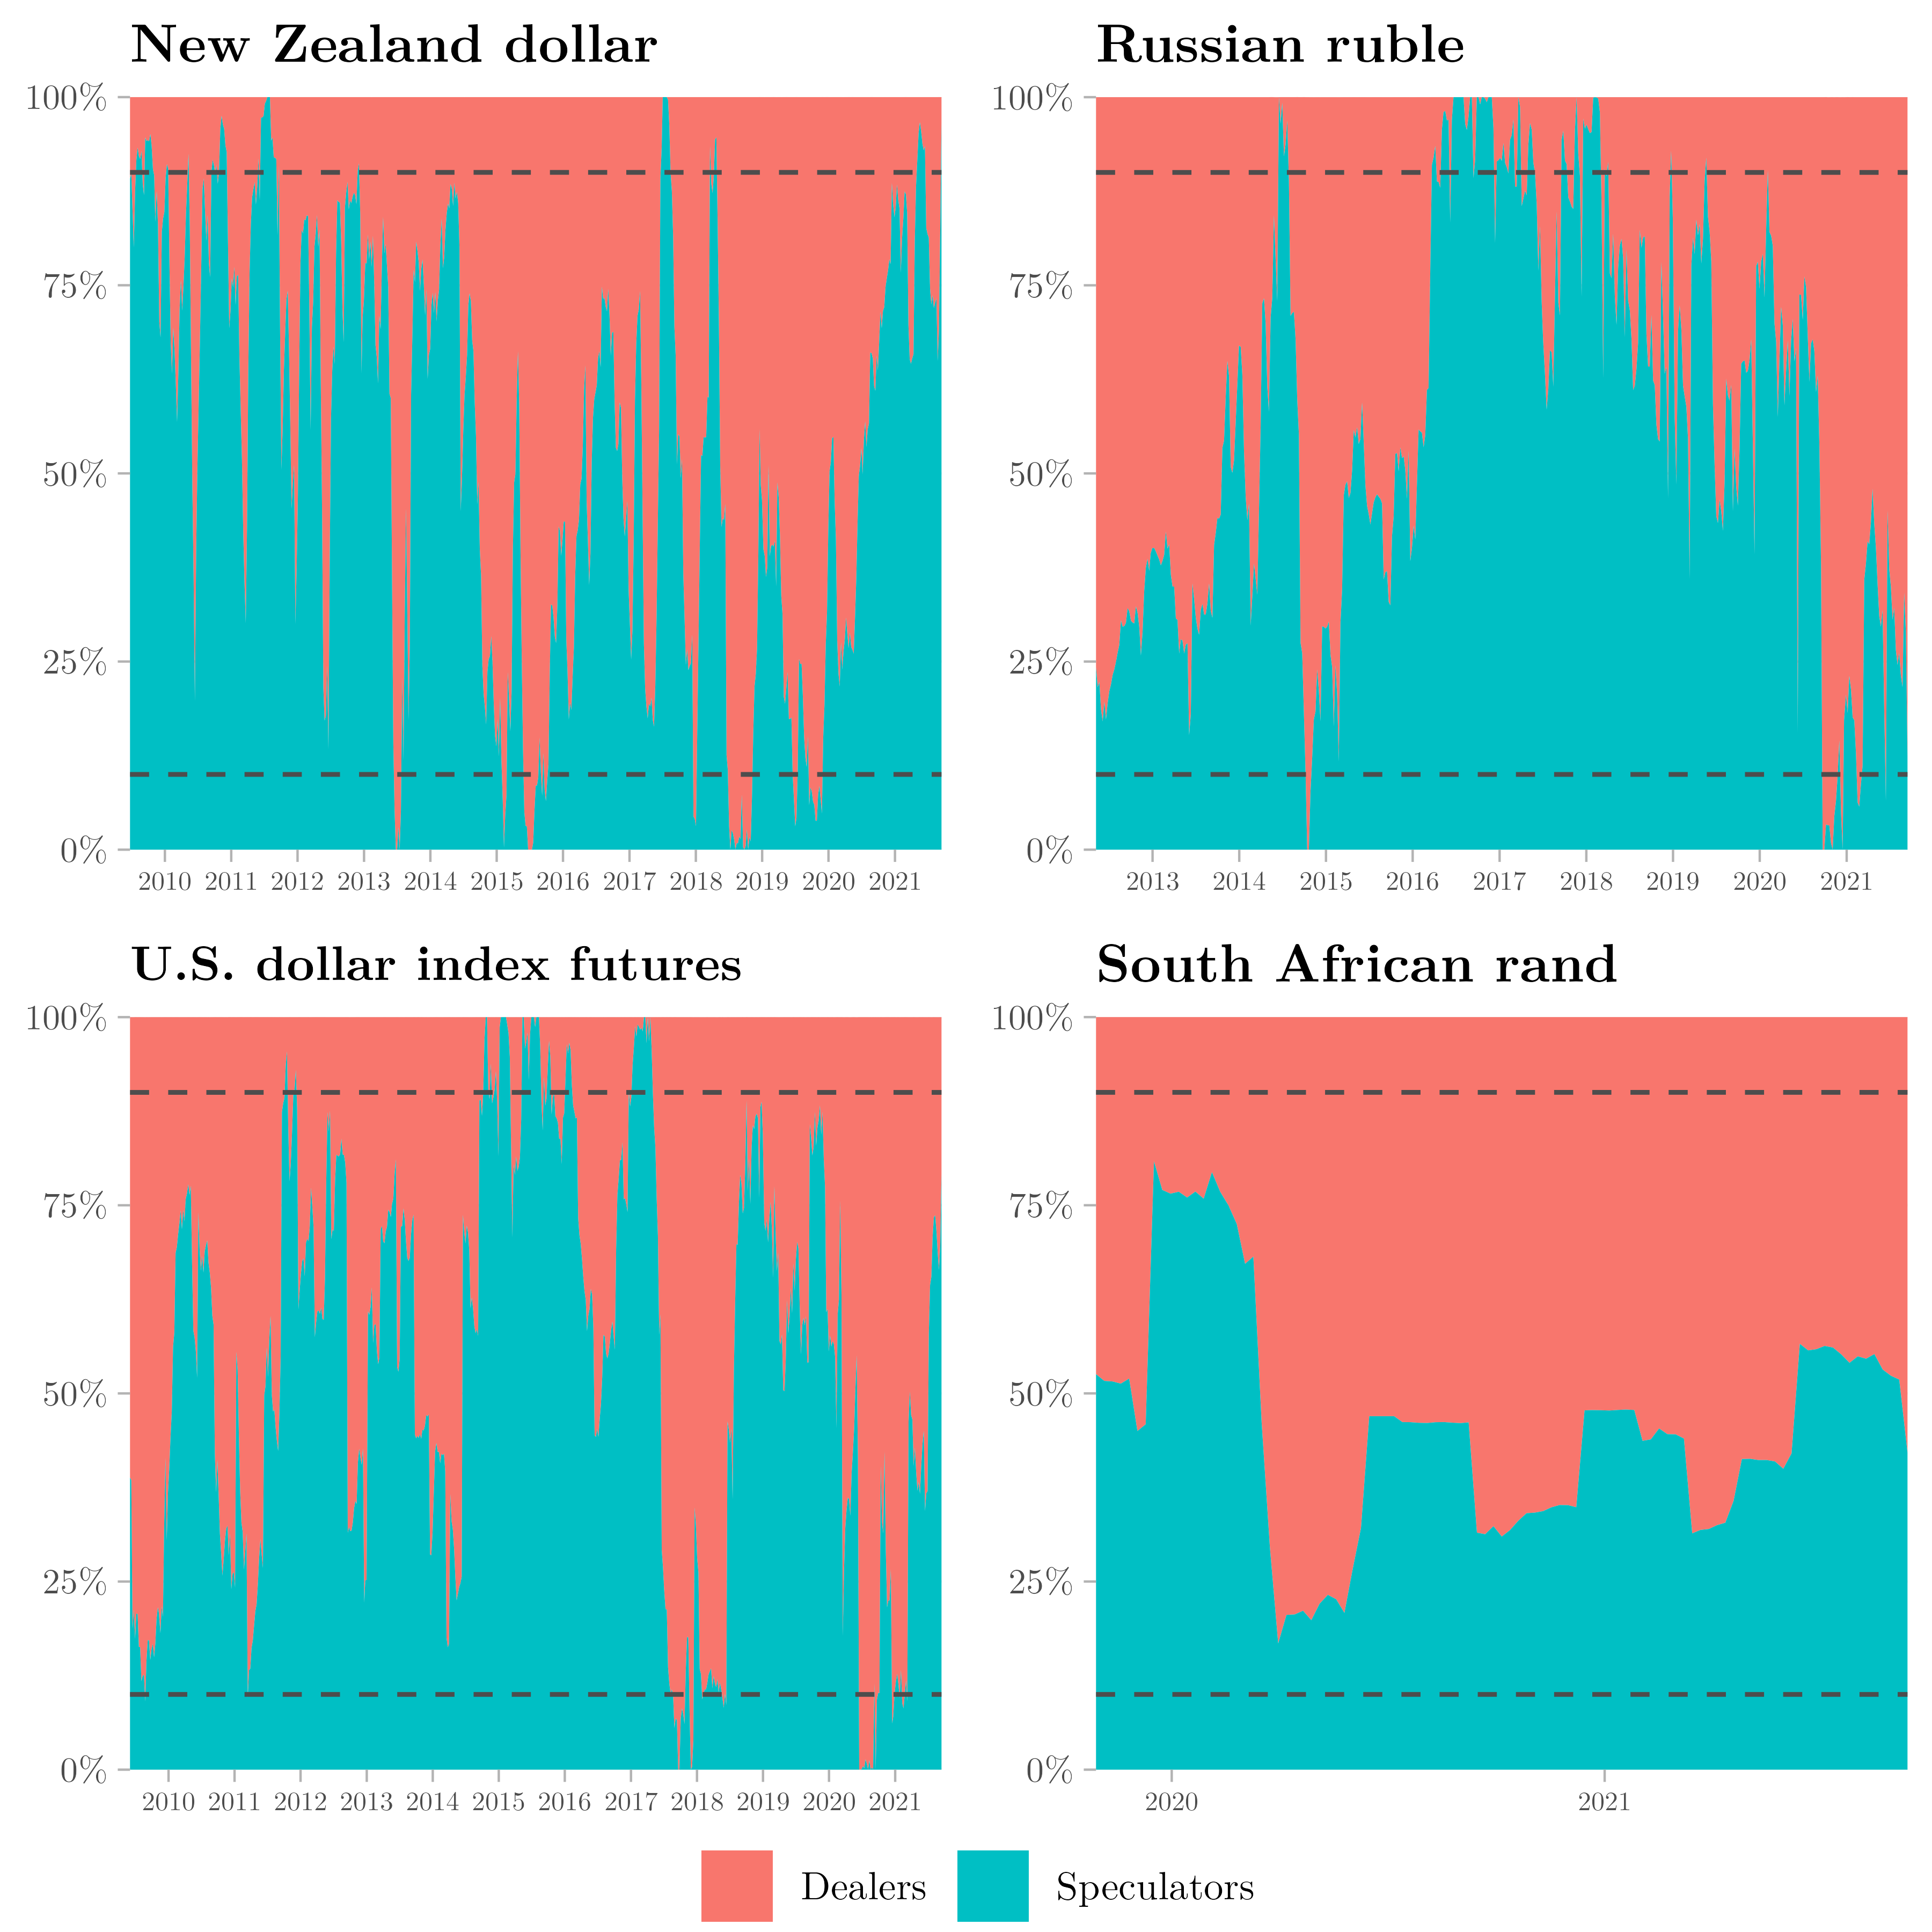
\includegraphics[width=0.99\columnwidth]{figure/OTHERCUR_2} 

}

\caption[Sentiment index for New Zealand dollar (2009-06-02 to 2021-09-21), Russian ruble (2012-05-08 to 2021-09-21), U.S. dollar index futures (2009-06-02 to 2021-09-21) and South African rand (2019-10-29 to 2021-09-21), three-year percentile]{Sentiment index for New Zealand dollar (2009-06-02 to 2021-09-21), Russian ruble (2012-05-08 to 2021-09-21), U.S. dollar index futures (2009-06-02 to 2021-09-21) and South African rand (2019-10-29 to 2021-09-21), three-year percentile \\ \scriptsize \textit{Source:} Commodity Futures Trading Commission (CFTC).}\label{fig:FigureA37}
\end{figure}

\clearpage

\hypertarget{appendixa5}{%
\section{Hedge fund net positions and interest rate differentials for other currencies}\label{appendixa5}}

\begin{figure}[!ht]

{\centering 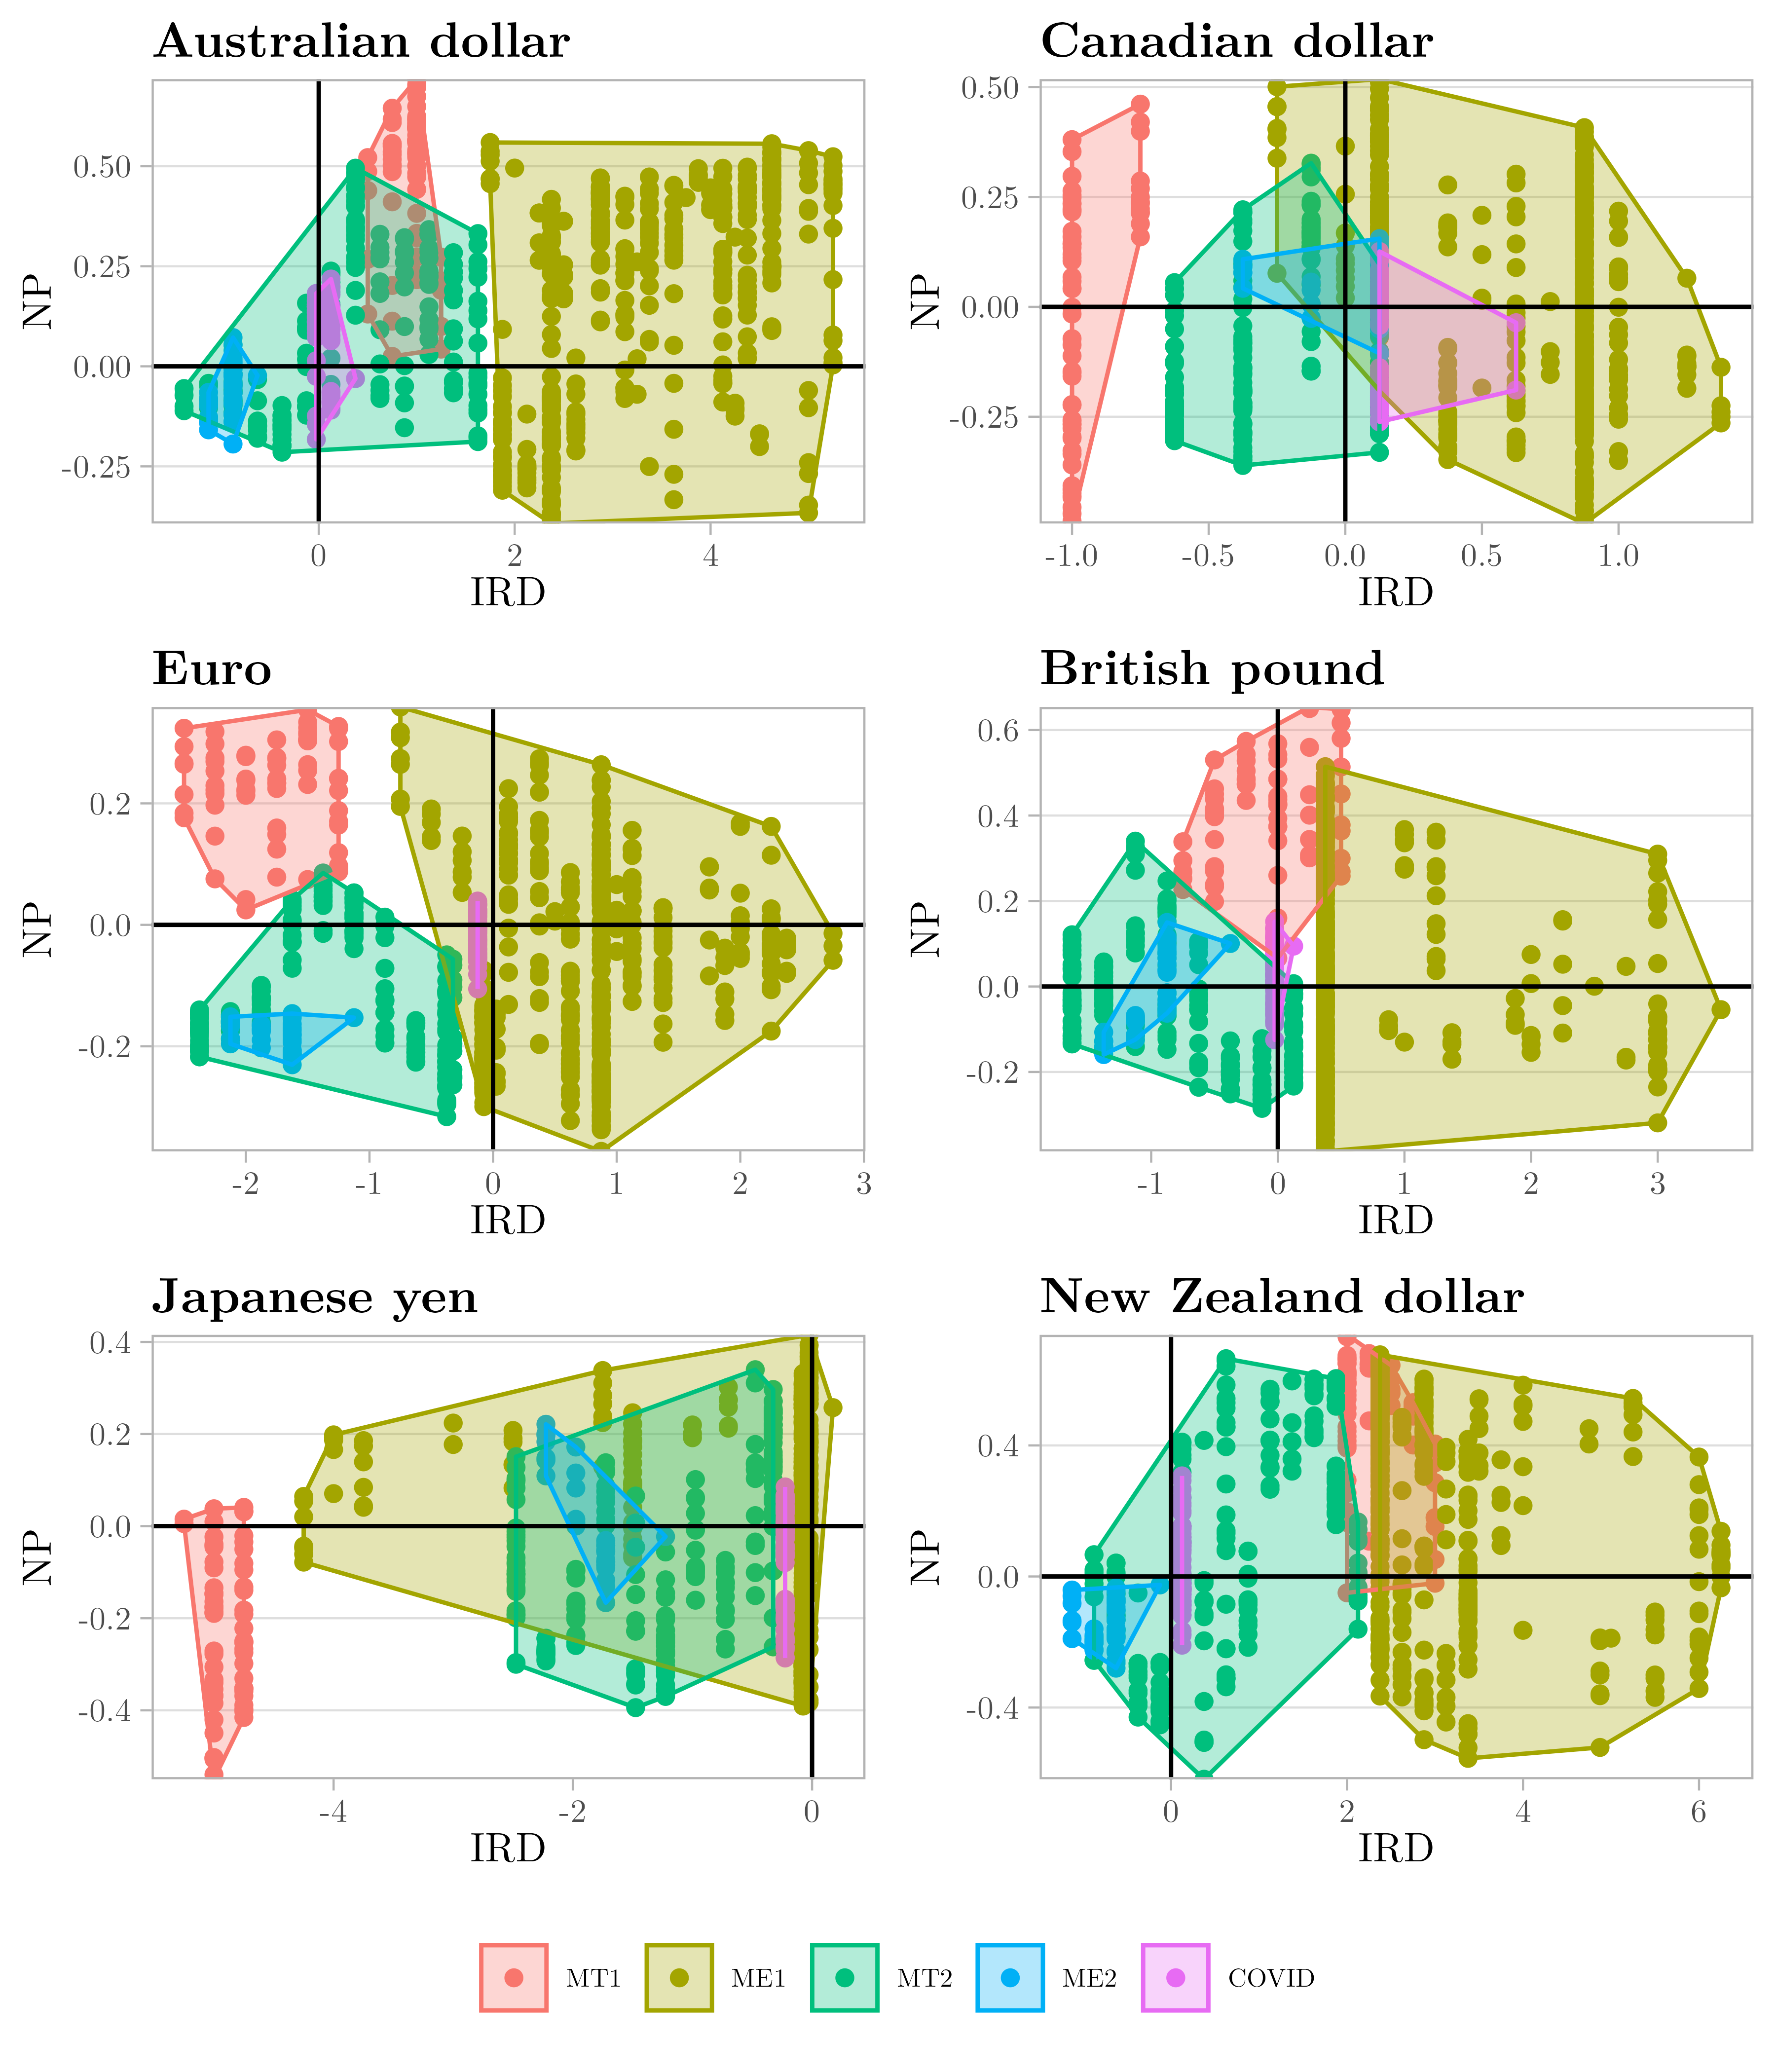
\includegraphics[width=0.99\columnwidth]{figure/OTHERCUR1_HF} 

}

\caption[Australian dollar, Canadian dollar, Euro, British pound, Japanese yen and New Zealand dollar, 2006-06-13 to 2021-09-21]{Hedge funds net positions and interest rate differentials for developed countries: Australian dollar, Canadian dollar, Euro, British pound, Japanese yen and New Zealand dollar, 2006-06-13 to 2021-09-21 \\ \scriptsize \textit{Source:} Commodity Futures Trading Comission (CFTC) and Bank for International Settlements (BIS).}\label{fig:FigureA38}
\end{figure}

\clearpage

\begin{figure}[!ht]

{\centering 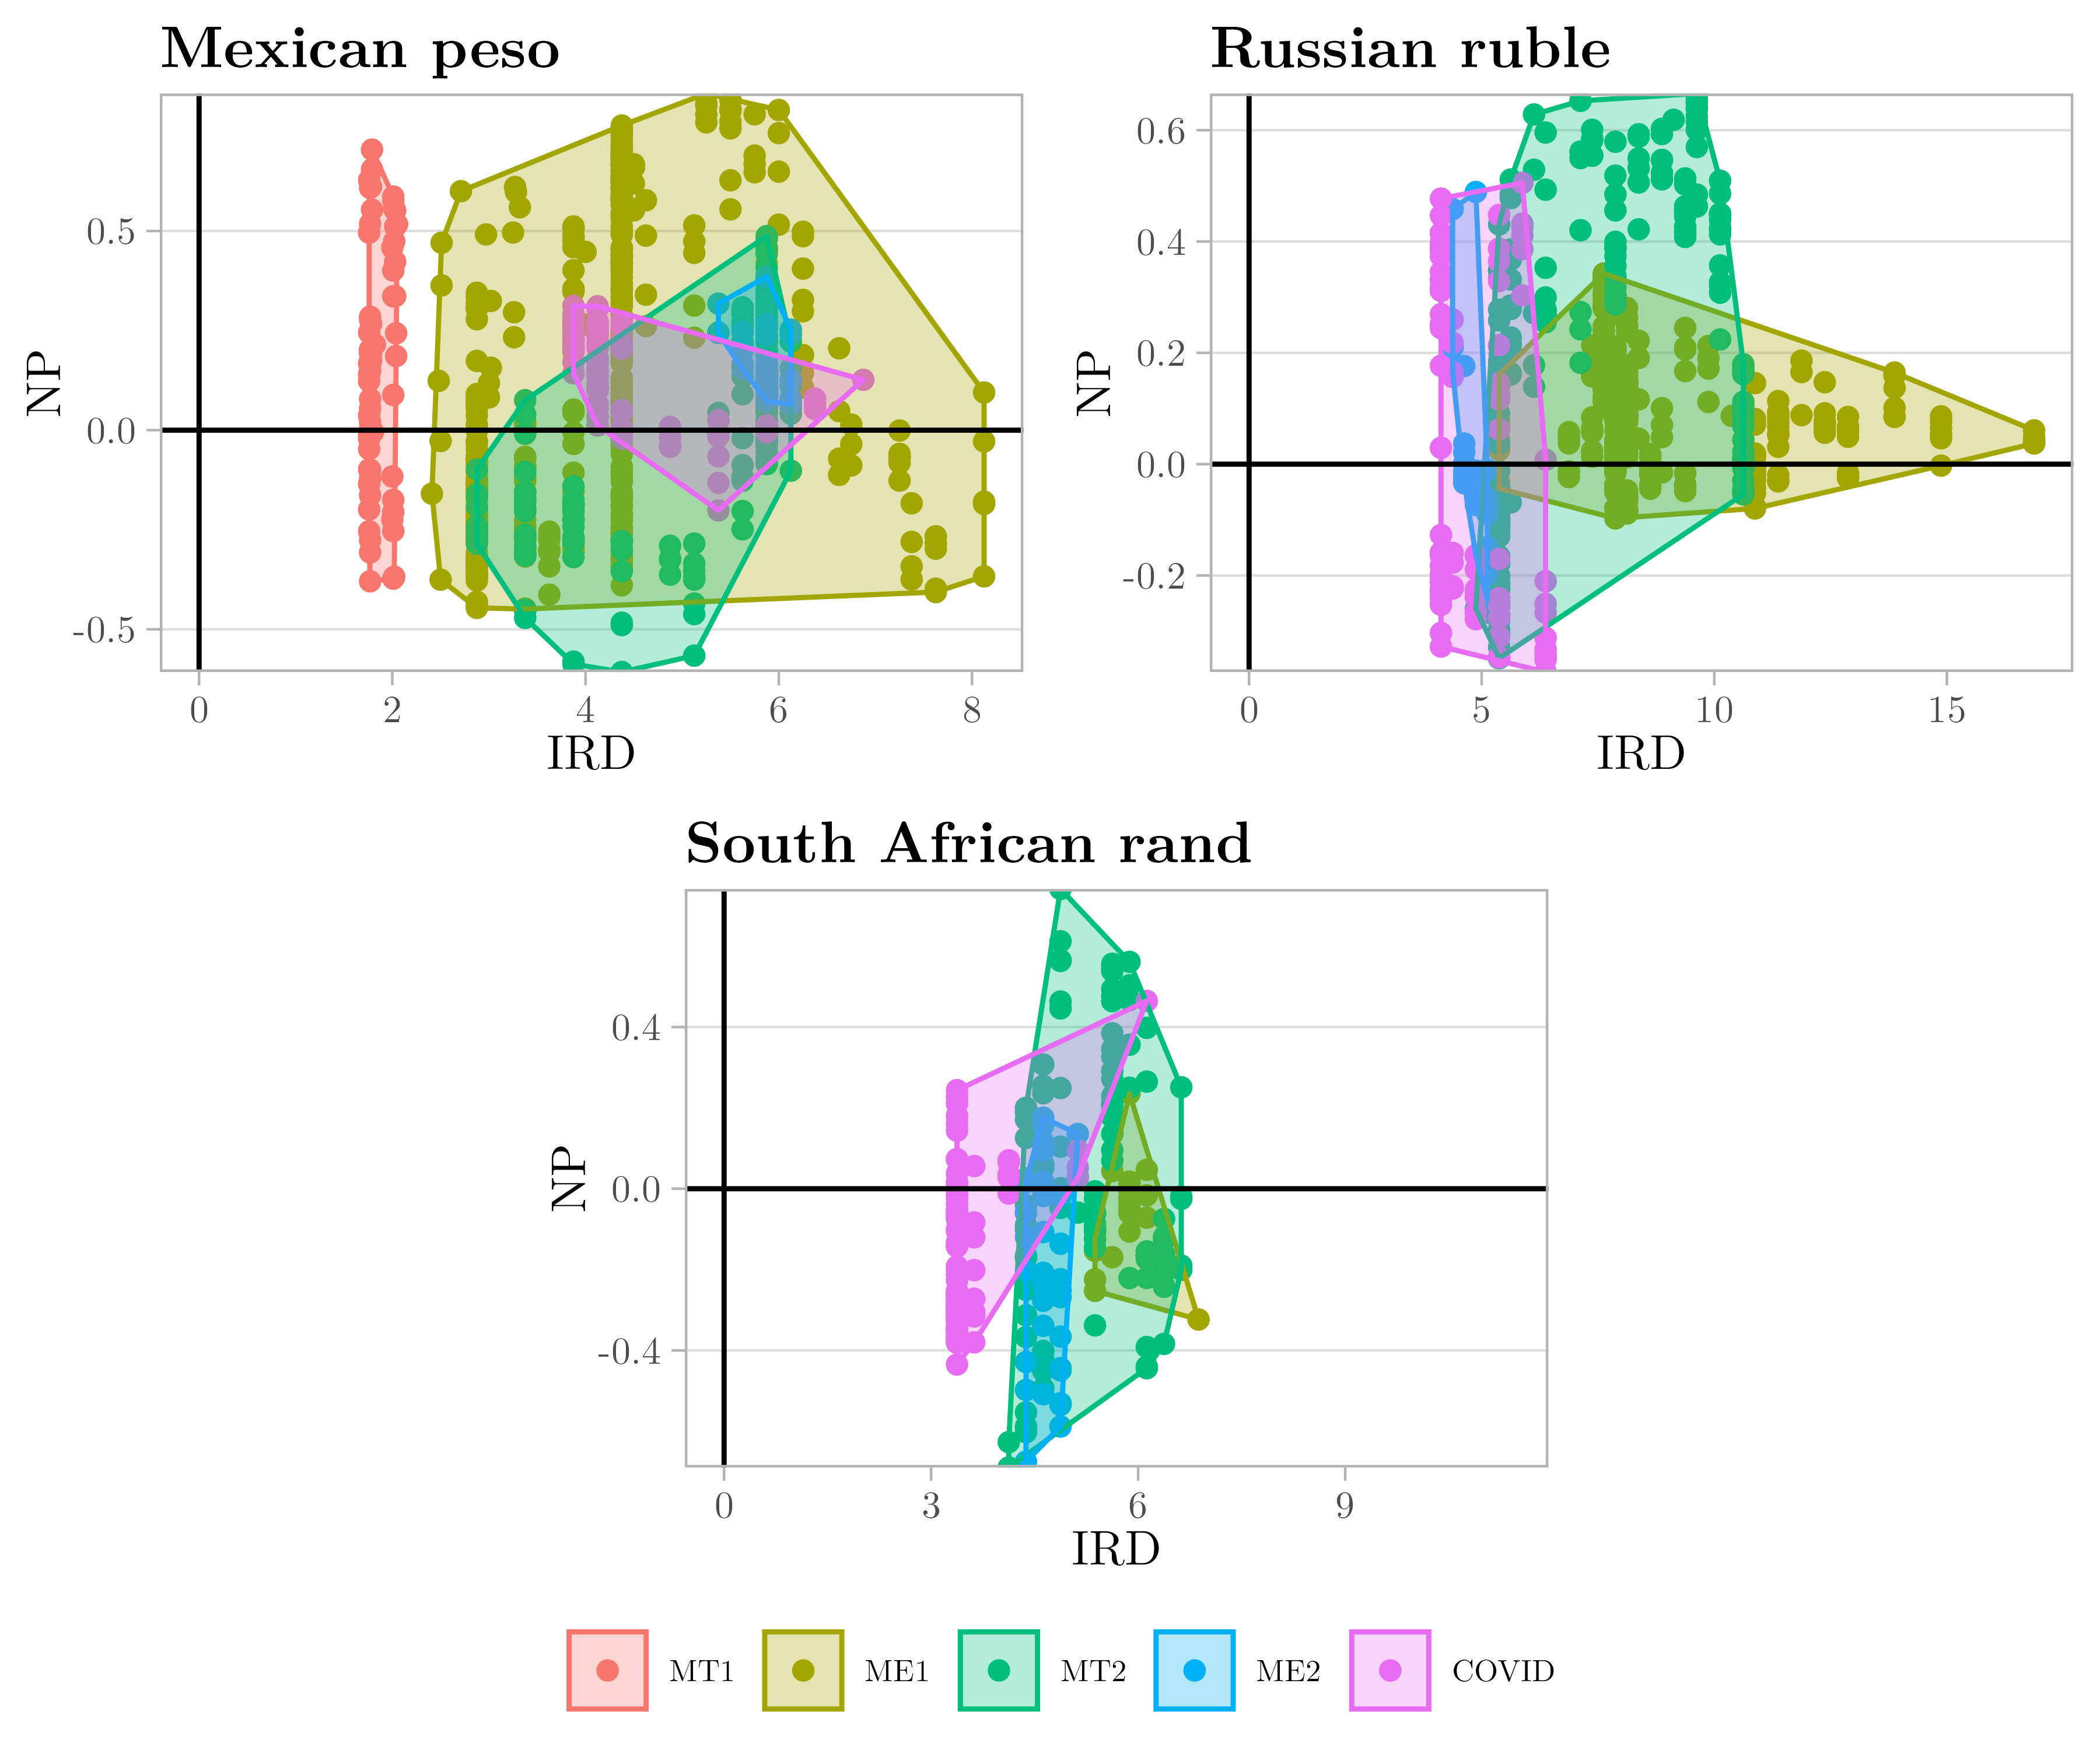
\includegraphics[width=0.99\columnwidth]{figure/OTHERCUR2_HF} 

}

\caption[Hedge funds net positions and interest rate differentials for developing countries: Mexican peso (2006-06-13 to 2021-09-21), Russian ruble (2009-02-10 to 2021-09-21) and South African rand (2015-05-26 to 2021-09-21)]{Hedge funds net positions and interest rate differentials for developing countries: Mexican peso (2006-06-13 to 2021-09-21), Russian ruble (2009-02-10 to 2021-09-21) and South African rand (2015-05-26 to 2021-09-21) \\ \scriptsize \textit{Source:} Commodity Futures Trading Comission (CFTC) and Bank for International Settlements (BIS).}\label{fig:FigureA39}
\end{figure}

\clearpage

\hypertarget{appendixb}{%
\chapter{Supplemental Material for Chapter 2}\label{appendixb}}

\hypertarget{appendixb1}{%
\section{VAR model equations}\label{appendixb1}}

\begingroup\small

\begin{equation}
  \begin{aligned}
ER_t 
= & \lambda_1 + \sum_{i=0}^k\alpha_{11i}ER_{t-1} + \sum_{j=k+1}^p\alpha_{12j}ER_{t-j} + \sum_{i=0}^k\beta_{11i}CT_{t-1} + \sum_{j=k+1}^p\beta_{12j}CT_{t-j} \\
+ & \sum_{i=0}^k\gamma_{11i}IRD_{t-1} + \sum_{j=k+1}^p\gamma_{12j}IRD_{t-j} + \sum_{i=0}^k\delta_{11i}VIX_{t-1} + \sum_{j=k+1}^p\delta_{12j}VIX_{t-j} \\
+ & \sum_{i=0}^k\phi_{11i}SM_{t-1} + \sum_{j=k+1}^p\phi_{12j}SM_{t-j} + \sum_{i=0}^k\psi_{11i}SMUS_{t-1} + \sum_{j=k+1}^p\psi_{12j}SMUS_{t-j} +\varepsilon_{1t}
  \end{aligned}
\label{eq:b1}
\end{equation}
\endgroup

\begingroup\small

\begin{equation}
  \begin{aligned}
CT_t 
= & \lambda_2 + \sum_{i=0}^k\beta_{21i}CT_{t-1} + \sum_{j=k+1}^p\beta_{22j}CT_{t-j} + \sum_{i=0}^k\alpha_{21i}ER_{t-1} + \sum_{j=k+1}^p\alpha_{22j}ER_{t-j} \\
+ & \sum_{i=0}^k\gamma_{21i}IRD_{t-1} + \sum_{j=k+1}^p\gamma_{22j}IRD_{t-j} + \sum_{i=0}^k\delta_{21i}VIX_{t-1} + \sum_{j=k+1}^p\delta_{22j}VIX_{t-j} \\
+ & \sum_{i=0}^k\phi_{21i}SM_{t-1} + \sum_{j=k+1}^p\phi_{22j}SM_{t-j} + \sum_{i=0}^k\psi_{21i}SMUS_{t-1} + \sum_{j=k+1}^p\psi_{22j}SMUS_{t-j} +\varepsilon_{2t}
  \end{aligned}
\label{eq:b2}
\end{equation}
\endgroup

\clearpage

\begingroup\small

\begin{equation}
  \begin{aligned}
IRD_t 
= & \lambda_3 + \sum_{i=0}^k\gamma_{31i}IRD_{t-1} + \sum_{j=k+1}^p\gamma_{32j}IRD_{t-j} + \sum_{i=0}^k\alpha_{31i}ER_{t-1} + \sum_{j=k+1}^p\alpha_{32j}ER_{t-j} \\
+ & \sum_{i=0}^k\beta_{31i}CT_{t-1} + \sum_{j=k+1}^p\beta_{32j}CT_{t-j} + \sum_{i=0}^k\delta_{31i}VIX_{t-1} + \sum_{j=k+1}^p\delta_{32j}VIX_{t-j} \\
+ & \sum_{i=0}^k\phi_{31i}SM_{t-1} + \sum_{j=k+1}^p\phi_{32j}SM_{t-j} + \sum_{i=0}^k\psi_{31i}SMUS_{t-1} + \sum_{j=k+1}^p\psi_{32j}SMUS_{t-j} +\varepsilon_{3t}
  \end{aligned}
\label{eq:b3}
\end{equation}
\endgroup

\begingroup\small

\begin{equation}
  \begin{aligned}
VIX_t 
= & \lambda_4 + \sum_{i=0}^k\delta_{41i}VIX_{t-1} + \sum_{j=k+1}^p\delta_{42j}VIX_{t-j} + \sum_{i=0}^k\alpha_{41i}ER_{t-1} + \sum_{j=k+1}^p\alpha_{42j}ER_{t-j} \\
+ & \sum_{i=0}^k\beta_{41i}CT_{t-1} + \sum_{j=k+1}^p\beta_{42j}CT_{t-j} + \sum_{i=0}^k\gamma_{41i}IRD_{t-1} + \sum_{j=k+1}^p\gamma_{42j}IRD_{t-j} \\
+ & \sum_{i=0}^k\phi_{41i}SM_{t-1} + \sum_{j=k+1}^p\phi_{42j}SM_{t-j} + \sum_{i=0}^k\psi_{41i}SMUS_{t-1} + \sum_{j=k+1}^p\psi_{42j}SMUS_{t-j} +\varepsilon_{4t}
  \end{aligned}
\label{eq:b4}
\end{equation}
\endgroup

\begingroup\small

\begin{equation}
  \begin{aligned}
SM_t 
= & \lambda_5 + \sum_{i=0}^k\phi_{51i}SM_{t-1} + \sum_{j=k+1}^p\phi_{52j}SM_{t-j} + \sum_{i=0}^k\alpha_{51i}ER_{t-1} + \sum_{j=k+1}^p\alpha_{52j}ER_{t-j} \\
+ & \sum_{i=0}^k\beta_{51i}CT_{t-1} + \sum_{j=k+1}^p\beta_{52j}CT_{t-j} + \sum_{i=0}^k\gamma_{51i}IRD_{t-1} + \sum_{j=k+1}^p\gamma_{52j}IRD_{t-j} \\
+ & \sum_{i=0}^k\delta_{51i}VIX_{t-1} + \sum_{j=k+1}^p\delta_{52j}VIX_{t-j} + \sum_{i=0}^k\psi_{51i}SMUS_{t-1} + \sum_{j=k+1}^p\psi_{52j}SMUS_{t-j} +\varepsilon_{5t}
  \end{aligned}
\label{eq:b5}
\end{equation}
\endgroup

\begingroup\small

\begin{equation}
  \begin{aligned}
SMUS_t 
= & \lambda_6 + \sum_{i=0}^k\psi_{61i}SMUS_{t-1} + \sum_{j=k+1}^p\psi_{62j}SMUS_{t-j} + \sum_{i=0}^k\alpha_{61i}ER_{t-1} + \sum_{j=k+1}^p\alpha_{62j}ER_{t-j} \\
+ & \sum_{i=0}^k\beta_{61i}CT_{t-1} + \sum_{j=k+1}^p\beta_{62j}CT_{t-j} + \sum_{i=0}^k\gamma_{61i}IRD_{t-1} + \sum_{j=k+1}^p\gamma_{62j}IRD_{t-j} \\
+ & \sum_{i=0}^k\delta_{61i}VIX_{t-1} + \sum_{j=k+1}^p\delta_{62j}VIX_{t-j} + \sum_{i=0}^k\phi_{61i}SM_{t-1} + \sum_{j=k+1}^p\phi_{62j}SM_{t-j} +\varepsilon_{6t}
  \end{aligned}
\label{eq:b6}
\end{equation}
\endgroup

\clearpage

\hypertarget{appendixb2}{%
\section{Descriptive statistics}\label{appendixb2}}

\begin{table}[H]

\caption{\label{tab:TableA21}Descriptive statistics for Australia}
\centering
\resizebox{\linewidth}{!}{
\begin{tabular}[t]{ccccccccccccccccccc}
\toprule
\multicolumn{1}{c}{ } & \multicolumn{6}{c}{ME} & \multicolumn{6}{c}{MTT} & \multicolumn{6}{c}{MTF} \\
\cmidrule(l{3pt}r{3pt}){2-7} \cmidrule(l{3pt}r{3pt}){8-13} \cmidrule(l{3pt}r{3pt}){14-19}
 & $CT$ & $ER$ & $IRD$ & $$VIX$$ & $SM$ & $SMUS$ & $CT$ & $ER$ & $IRD$ & $$VIX$$ & $SM$ & $SMUS$ & $CTF$ & $ER$ & $IRDF$ & $$VIX$$ & $SM$ & $SMUS$\\
\midrule
Observations & 364 & 364 & 364 & 364 & 364 & 364 & 118 & 118 & 118 & 118 & 118 & 118 & 66 & 66 & 66 & 66 & 66 & 66\\
Mean & 2.90 & 0.92 & 3.22 & 20.27 & 4,791.42 & 1,479.75 & 1.78 & 0.76 & 0.87 & 13.88 & 5,574.18 & 2,314.64 & 2.80 & 0.72 & 0.59 & 16.52 & 6,077.30 & 2,764.88\\
Std. Deviation & 2.87 & 0.11 & 0.93 & 8.06 & 588.45 & 393.13 & 0.82 & 0.02 & 0.51 & 4.12 & 321.85 & 244.30 & 1.03 & 0.02 & 0.31 & 4.34 & 255.83 & 118.89\\
Min. & 0.12 & 0.64 & 1.88 & 10.99 & 3,184.50 & 696.33 & 0.56 & 0.69 & 0.12 & 9.43 & 4,832.10 & 1,852.21 & 0.84 & 0.69 & 0.12 & 10.93 & 5,493.80 & 2,351.10\\
Max. & 14.94 & 1.10 & 4.63 & 56.65 & 5,969.10 & 2,480.64 & 3.93 & 0.81 & 1.62 & 29.98 & 6,135.80 & 2,839.13 & 5.43 & 0.78 & 1.12 & 36.07 & 6,658.00 & 2,945.83\\
\bottomrule
\end{tabular}}
\end{table}

\begin{table}[H]

\caption{\label{tab:TableA22}Descriptive statistics for Brazil}
\centering
\resizebox{\linewidth}{!}{
\begin{tabular}[t]{ccccccccccccc}
\toprule
\multicolumn{1}{c}{ } & \multicolumn{6}{c}{ME} & \multicolumn{6}{c}{MT} \\
\cmidrule(l{3pt}r{3pt}){2-7} \cmidrule(l{3pt}r{3pt}){8-13}
 & $CT$ & $ER$ & $IRD$ & $VIX$ & $SM$ & $SMUS$ & $CT$ & $ER$ & $IRD$ & $VIX$ & $SM$ & $SMUS$\\
\midrule
Observations & 94 & 94 & 94 & 94 & 94 & 94 & 184 & 184 & 184 & 184 & 184 & 184\\
Mean & 1.35 & 2.83 & 12.08 & 35.54 & 52,061.26 & 1,994.08 & 2.15 & 3.50 & 8.61 & 35.30 & 71,185.65 & 2,476.14\\
Std. Deviation & 0.99 & 0.59 & 1.42 & 9.90 & 5,491.30 & 94.00 & 2.24 & 0.32 & 4.06 & 7.12 & 15,386.76 & 300.11\\
Min. & 0.08 & 2.20 & 9.88 & 22.58 & 44,132.00 & 1,755.20 & 0.16 & 3.07 & 4.12 & 24.19 & 37,497.00 & 1,852.21\\
Max. & 3.99 & 4.09 & 14.12 & 67.66 & 72,583.00 & 2,127.83 & 11.51 & 4.18 & 13.88 & 57.79 & 100,093.00 & 2,945.83\\
\bottomrule
\end{tabular}}
\end{table}

\begin{table}[H]

\caption{\label{tab:TableA23}Descriptive statistics for Canada}
\centering
\resizebox{\linewidth}{!}{
\begin{tabular}[t]{ccccccccccccc}
\toprule
\multicolumn{1}{c}{ } & \multicolumn{6}{c}{ME} & \multicolumn{6}{c}{MT} \\
\cmidrule(l{3pt}r{3pt}){2-7} \cmidrule(l{3pt}r{3pt}){8-13}
 & $CT$ & $ER$ & $IRD$ & $VIX$ & $SM$ & $SMUS$ & $CTF$ & $ER$ & $IRDF$ & $VIX$ & $SM$ & $SMUS$\\
\midrule
Observations & 364 & 364 & 364 & 364 & 364 & 364 & 184 & 184 & 184 & 184 & 184 & 184\\
Mean & 2.80 & 1.08 & 0.69 & 20.27 & 12,697.83 & 1,479.75 & 1.64 & 1.31 & 0.24 & 14.83 & 15,162.19 & 2,476.14\\
Std. Deviation & 4.19 & 0.10 & 0.30 & 8.06 & 1,573.97 & 393.13 & 1.14 & 0.04 & 0.28 & 4.38 & 1,071.97 & 300.11\\
Min. & 0.20 & 0.94 & 0.12 & 10.99 & 7,631.60 & 696.33 & 0.21 & 1.21 & -0.12 & 9.43 & 12,002.20 & 1,852.21\\
Max. & 32.23 & 1.37 & 1.38 & 56.65 & 15,619.20 & 2,480.64 & 5.14 & 1.45 & 0.62 & 36.07 & 16,669.40 & 2,945.83\\
\bottomrule
\end{tabular}}
\end{table}

\begin{table}[H]

\caption{\label{tab:TableA24}Descriptive statistics for Euro area countries}
\centering
\resizebox{\linewidth}{!}{
\begin{tabular}[t]{ccccccccccccc}
\toprule
\multicolumn{1}{c}{ } & \multicolumn{6}{c}{ME} & \multicolumn{6}{c}{MT} \\
\cmidrule(l{3pt}r{3pt}){2-7} \cmidrule(l{3pt}r{3pt}){8-13}
 & $CT$ & $ER$ & $IRD$ & $VIX$ & $SM$ & $SMUS$ & $CTF$ & $ER$ & $IRDF$ & $VIX$ & $SM$ & $SMUS$\\
\midrule
Observations & 364 & 364 & 364 & 364 & 364 & 364 & 184 & 184 & 184 & 184 & 184 & 184\\
Mean & 0.84 & 1.31 & 0.62 & 11.53 & 720.28 & 1,479.75 & 1.22 & 1.14 & 1.22 & 8.35 & 971.35 & 2,476.14\\
Std. Deviation & 0.69 & 0.10 & 0.51 & 3.59 & 125.70 & 393.13 & 0.63 & 0.05 & 0.74 & 1.75 & 80.85 & 300.11\\
Min. & 0.15 & 1.06 & -0.08 & 4.84 & 439.82 & 696.33 & 0.37 & 1.04 & 0.32 & 4.99 & 788.87 & 1,852.21\\
Max. & 4.44 & 1.51 & 2.38 & 26.25 & 1,020.33 & 2,480.64 & 3.40 & 1.25 & 2.38 & 14.49 & 1,088.01 & 2,945.83\\
\bottomrule
\end{tabular}}
\end{table}

\begin{table}[H]

\caption{\label{tab:TableA25}Descriptive statistics for Japan}
\centering
\resizebox{\linewidth}{!}{
\begin{tabular}[t]{ccccccccccccc}
\toprule
\multicolumn{1}{c}{ } & \multicolumn{6}{c}{ME} & \multicolumn{6}{c}{MT} \\
\cmidrule(l{3pt}r{3pt}){2-7} \cmidrule(l{3pt}r{3pt}){8-13}
 & $CTF$ & $ER$ & $IRDF$ & $VIX$ & $SM$ & $SMUS$ & $CTF$ & $ER$ & $IRDF$ & $VIX$ & $SM$ & $SMUS$\\
\midrule
Observations & 364 & 364 & 364 & 364 & 364 & 364 & 184 & 184 & 184 & 184 & 184 & 184\\
Mean & 2.48 & 94.88 & 0.06 & 20.27 & 12,512.70 & 1,479.75 & 2.21 & 110.52 & 1.29 & 14.83 & 19,983.68 & 2,476.14\\
Std. Deviation & 2.41 & 14.15 & 0.02 & 8.06 & 3,814.30 & 393.13 & 1.40 & 3.85 & 0.77 & 4.38 & 2,324.69 & 300.11\\
Min. & 0.18 & 76.15 & 0.03 & 10.99 & 7,054.98 & 696.33 & 0.27 & 99.81 & 0.32 & 9.43 & 15,323.14 & 1,852.21\\
Max. & 12.36 & 124.82 & 0.08 & 56.65 & 20,841.97 & 2,480.64 & 5.84 & 120.91 & 2.47 & 36.07 & 24,270.62 & 2,945.83\\
\bottomrule
\end{tabular}}
\end{table}

\clearpage

\begin{table}[H]

\caption{\label{tab:TableA26}Descriptive statistics for Mexico}
\centering
\resizebox{\linewidth}{!}{
\begin{tabular}[t]{ccccccccccccc}
\toprule
\multicolumn{1}{c}{ } & \multicolumn{6}{c}{ME} & \multicolumn{6}{c}{MT} \\
\cmidrule(l{3pt}r{3pt}){2-7} \cmidrule(l{3pt}r{3pt}){8-13}
 & $CT$ & $ER$ & $IRD$ & $VIX$ & $SM$ & $SMUS$ & $CT$ & $ER$ & $IRD$ & $VIX$ & $SM$ & $SMUS$\\
\midrule
Observations & 364 & 364 & 364 & 364 & 364 & 364 & 184 & 184 & 184 & 184 & 184 & 184\\
Mean & 6.32 & 13.37 & 4.07 & 20.27 & 37,404.53 & 1,479.75 & 1.89 & 18.94 & 5.19 & 14.83 & 46,561.35 & 2,476.14\\
Std. Deviation & 8.60 & 1.19 & 0.98 & 8.06 & 6,558.44 & 393.13 & 1.66 & 0.87 & 1.02 & 4.38 & 2,942.66 & 300.11\\
Min. & 0.15 & 11.58 & 2.88 & 10.99 & 17,093.25 & 696.33 & 0.16 & 17.11 & 2.88 & 9.43 & 36,636.70 & 1,852.21\\
Max. & 65.06 & 17.26 & 8.12 & 56.65 & 45,915.17 & 2,480.64 & 7.83 & 21.58 & 6.12 & 36.07 & 51,713.38 & 2,945.83\\
\bottomrule
\end{tabular}}
\end{table}

\begin{table}[H]

\caption{\label{tab:TableA27}Descriptive statistics for New Zealand}
\centering
\resizebox{\linewidth}{!}{
\begin{tabular}[t]{ccccccccccccccccccc}
\toprule
\multicolumn{1}{c}{ } & \multicolumn{6}{c}{ME} & \multicolumn{6}{c}{MTT} & \multicolumn{6}{c}{MTF} \\
\cmidrule(l{3pt}r{3pt}){2-7} \cmidrule(l{3pt}r{3pt}){8-13} \cmidrule(l{3pt}r{3pt}){14-19}
 & $CT$ & $ER$ & $IRD$ & $VIX$ & $SM$ & $SMUS$ & $CT$ & $ER$ & $IRD$ & $VIX$ & $SM$ & $SMUS$ & $CTF$ & $ER$ & $IRDF$ & $VIX$ & $SM$ & $SMUS$\\
\midrule
Observations & 364 & 364 & 364 & 364 & 364 & 364 & 130 & 130 & 130 & 130 & 130 & 130 & 54 & 54 & 54 & 54 & 54 & 54\\
Mean & 3.89 & 0.76 & 2.67 & 20.27 & 4,164.54 & 1,479.75 & 1.30 & 0.71 & 1.11 & 14.12 & 7,505.53 & 2,348.77 & 2.08 & 0.67 & 0.46 & 16.55 & 9,276.32 & 2,782.76\\
Std. Deviation & 4.74 & 0.08 & 0.45 & 8.06 & 1,267.59 & 393.13 & 1.06 & 0.02 & 0.65 & 4.12 & 831.67 & 256.76 & 1.05 & 0.01 & 0.26 & 4.54 & 504.01 & 122.24\\
Min. & 0.21 & 0.49 & 2.38 & 10.99 & 2,417.95 & 696.33 & 0.48 & 0.64 & 0.12 & 9.43 & 6,071.31 & 1,852.21 & 0.78 & 0.65 & 0.12 & 10.93 & 8,648.38 & 2,351.10\\
Max. & 42.53 & 0.88 & 4.88 & 56.65 & 9,826.86 & 2,480.64 & 6.42 & 0.75 & 2.12 & 29.98 & 9,826.86 & 2,839.13 & 4.91 & 0.69 & 0.88 & 36.07 & 10,418.29 & 2,945.83\\
\bottomrule
\end{tabular}}
\end{table}

\begin{table}[H]

\caption{\label{tab:TableA28}Descriptive statistics for Russia}
\centering
\resizebox{\linewidth}{!}{
\begin{tabular}[t]{ccccccccccccc}
\toprule
\multicolumn{1}{c}{ } & \multicolumn{6}{c}{ME} & \multicolumn{6}{c}{MT} \\
\cmidrule(l{3pt}r{3pt}){2-7} \cmidrule(l{3pt}r{3pt}){8-13}
 & $CT$ & $ER$ & $IRD$ & $VIX$ & $SM$ & $SMUS$ & $CT$ & $ER$ & $IRD$ & $VIX$ & $SM$ & $SMUS$\\
\midrule
Observations & 315 & 315 & 315 & 315 & 315 & 315 & 184 & 184 & 184 & 184 & 184 & 184\\
Mean & 32.67 & 36.78 & 8.64 & 18.55 & 1,508.05 & 1,551.34 & 9.80 & 63.17 & 7.66 & 14.83 & 2,163.53 & 2,476.14\\
Std. Deviation & 153.30 & 11.71 & 2.20 & 5.91 & 156.29 & 355.36 & 23.58 & 5.01 & 2.05 & 4.38 & 240.44 & 300.11\\
Min. & 0.00 & 27.38 & 5.38 & 10.99 & 1,197.39 & 1,028.06 & 0.00 & 55.93 & 5.12 & 9.43 & 1,645.56 & 1,852.21\\
Max. & 1,485.80 & 73.00 & 16.88 & 40.82 & 2,286.40 & 2,480.64 & 190.74 & 80.07 & 10.62 & 36.07 & 2,761.69 & 2,945.83\\
\bottomrule
\end{tabular}}
\end{table}

\begin{table}[H]

\caption{\label{tab:TableA29}Descriptive statistics for Switzerland}
\centering
\resizebox{\linewidth}{!}{
\begin{tabular}[t]{ccccccccccccc}
\toprule
\multicolumn{1}{c}{ } & \multicolumn{6}{c}{ME} & \multicolumn{6}{c}{MT} \\
\cmidrule(l{3pt}r{3pt}){2-7} \cmidrule(l{3pt}r{3pt}){8-13}
 & $CTF$ & $ER$ & $IRDF$ & $VIX$ & $SM$ & $SMUS$ & $CTF$ & $ER$ & $IRDF$ & $VIX$ & $SM$ & $SMUS$\\
\midrule
Observations & 364 & 364 & 364 & 364 & 364 & 364 & 184 & 184 & 184 & 184 & 184 & 184\\
Mean & 1.55 & 0.97 & 0.02 & 20.27 & 7,128.30 & 1,479.75 & 2.66 & 0.99 & 1.97 & 14.83 & 8,706.81 & 2,476.14\\
Std. Deviation & 1.40 & 0.08 & 0.36 & 8.06 & 1,274.44 & 393.13 & 2.03 & 0.02 & 0.73 & 4.38 & 547.35 & 300.11\\
Min. & 0.09 & 0.74 & -0.38 & 10.99 & 4,358.00 & 696.33 & 0.53 & 0.93 & 1.12 & 9.43 & 7,583.27 & 1,852.21\\
Max. & 8.11 & 1.18 & 0.88 & 56.65 & 9,480.20 & 2,480.64 & 10.62 & 1.03 & 3.12 & 36.07 & 9,988.55 & 2,945.83\\
\bottomrule
\end{tabular}}
\end{table}

\begin{table}[H]

\caption{\label{tab:TableA210}Descriptive statistics for the United Kingdom}
\centering
\resizebox{\linewidth}{!}{
\begin{tabular}[t]{ccccccccccccc}
\toprule
\multicolumn{1}{c}{ } & \multicolumn{6}{c}{ME} & \multicolumn{6}{c}{MT} \\
\cmidrule(l{3pt}r{3pt}){2-7} \cmidrule(l{3pt}r{3pt}){8-13}
 & $CT$ & $ER$ & $IRD$ & $VIX$ & $SM$ & $SMUS$ & $CTF$ & $ER$ & $IRDF$ & $VIX$ & $SM$ & $SMUS$\\
\midrule
Observations & 364 & 364 & 364 & 364 & 364 & 364 & 184 & 184 & 184 & 184 & 184 & 184\\
Mean & 0.86 & 1.58 & 0.40 & 20.27 & 5,880.17 & 1,479.75 & 1.97 & 1.32 & 0.75 & 14.83 & 7,059.33 & 2,476.14\\
Std. Deviation & 0.59 & 0.06 & 0.16 & 8.06 & 769.00 & 393.13 & 0.85 & 0.07 & 0.60 & 4.38 & 533.27 & 300.11\\
Min. & 0.12 & 1.38 & 0.38 & 10.99 & 3,512.10 & 696.33 & 0.53 & 1.20 & -0.12 & 9.43 & 5,237.50 & 1,852.21\\
Max. & 4.22 & 1.71 & 1.88 & 56.65 & 7,075.30 & 2,480.64 & 4.32 & 1.49 & 1.62 & 36.07 & 7,877.50 & 2,945.83\\
\bottomrule
\end{tabular}}
\end{table}

\clearpage

\hypertarget{appendixb3}{%
\section{Unit-root tests (Clemente-Montañés-Reyes)}\label{appendixb3}}

\begin{table}[H]

\caption{\label{tab:TableB21}Unit-root tests for Australia}
\centering
\resizebox{\linewidth}{!}{
\begin{tabular}[t]{ccccccccccccccccccc}
\toprule
\multicolumn{1}{c}{ } & \multicolumn{6}{c}{ME} & \multicolumn{6}{c}{MTT} & \multicolumn{6}{c}{MTF} \\
\cmidrule(l{3pt}r{3pt}){2-7} \cmidrule(l{3pt}r{3pt}){8-13} \cmidrule(l{3pt}r{3pt}){14-19}
 & $CT$ & $ER$ & $IRD$ & $$VIX$$ & $SM$ & $SMUS$ & $CT$ & $ER$ & $IRD$ & $$VIX$$ & $SM$ & $SMUS$ & $CTF$ & $ER$ & $IRDF$ & $$VIX$$ & $SM$ & $SMUS$\\
\midrule
$(\rho - 1)$ & -0.16 & -0.03 & -0.02 & -0.11 & -0.11 & -0.04 & -0.19 & -0.17 & -0.12 & -0.27 & -0.37 & -0.04 & -0.29 & -0.38 & -0.16 & -0.32 & -0.11 & -0.09\\
t-stat & -3.68 & -2.86 & -2.02 & -3.97 & -3.41 & -1.95 & -2.95 & -3.38 & -2.08 & -4.15 & -5.18 & -2.18 & -3.27 & -3.98 & -1.66 & -4.62 & -1.93 & -1.64\\
Critical value & -3.61 & -3.61 & -3.61 & -3.61 & -3.61 & -3.61 & -3.56 & -3.56 & -3.56 & -3.56 & -3.56 & -3.56 & -3.65 & -3.65 & -3.65 & -3.65 & -3.65 & -3.65\\
I($d$) & I(0) & I(1) & I(1) & I(0) & I(1) & I(1) & I(1) & I(1) & I(1) & I(0) & I(0) & I(1) & I(1) & I(0) & I(1) & I(0) & I(1) & I(1)\\
T & 328 & 328 & 328 & 328 & 328 & 328 & 106 & 106 & 106 & 106 & 106 & 106 & 60 & 60 & 60 & 60 & 60 & 60\\
\bottomrule
\end{tabular}}
\end{table}

\begin{table}[H]

\caption{\label{tab:TableB22}Unit-root tests for Brazil}
\centering
\resizebox{\linewidth}{!}{
\begin{tabular}[t]{ccccccccccccc}
\toprule
\multicolumn{1}{c}{ } & \multicolumn{6}{c}{ME} & \multicolumn{6}{c}{MT} \\
\cmidrule(l{3pt}r{3pt}){2-7} \cmidrule(l{3pt}r{3pt}){8-13}
 & $CT$ & $ER$ & $IRD$ & $VIX$ & $SM$ & $SMUS$ & $CT$ & $ER$ & $IRD$ & $VIX$ & $SM$ & $SMUS$\\
\midrule
$(\rho - 1)$ & -0.22 & -0.21 & -0.18 & -0.27 & -0.35 & -0.28 & -0.15 & -0.08 & -0.10 & -0.19 & -0.07 & -0.07\\
t-stat & -1.78 & -2.72 & -2.91 & -3.84 & -1.79 & -4.06 & -3.08 & -3.24 & -2.40 & -3.09 & -1.44 & -2.60\\
Critical value & -3.56 & -3.56 & -3.56 & -3.56 & -3.56 & -3.56 & -3.56 & -3.56 & -3.56 & -3.56 & -3.56 & -3.56\\
I($d$) & I(1) & I(1) & I(1) & I(0) & I(1) & I(0) & I(1) & I(1) & I(1) & I(1) & I(1) & I(1)\\
T & 84 & 84 & 84 & 84 & 84 & 84 & 166 & 166 & 166 & 166 & 166 & 166\\
\bottomrule
\end{tabular}}
\end{table}

\begin{table}[H]

\caption{\label{tab:TableB23}Unit-root tests for Canada}
\centering
\resizebox{\linewidth}{!}{
\begin{tabular}[t]{ccccccccccccc}
\toprule
\multicolumn{1}{c}{ } & \multicolumn{6}{c}{ME} & \multicolumn{6}{c}{MT} \\
\cmidrule(l{3pt}r{3pt}){2-7} \cmidrule(l{3pt}r{3pt}){8-13}
 & $CT$ & $ER$ & $IRD$ & $VIX$ & $SM$ & $SMUS$ & $CTF$ & $ER$ & $IRDF$ & $VIX$ & $SM$ & $SMUS$\\
\midrule
$(\rho - 1)$ & -0.12 & -0.06 & -0.05 & -0.11 & -0.05 & -0.04 & -0.09 & -0.09 & -0.07 & -0.19 & -0.18 & -0.07\\
t-stat & -4.40 & -3.49 & -2.88 & -3.97 & -2.97 & -1.95 & -3.07 & -3.25 & -1.38 & -3.52 & -3.32 & -2.60\\
Critical value & -3.61 & -3.61 & -3.61 & -3.61 & -3.61 & -3.61 & -3.56 & -3.56 & -3.56 & -3.56 & -3.56 & -3.56\\
I($d$) & I(0) & I(1) & I(1) & I(0) & I(1) & I(1) & I(1) & I(1) & I(1) & I(1) & I(1) & I(1)\\
T & 328 & 328 & 328 & 328 & 328 & 328 & 166 & 166 & 166 & 166 & 166 & 166\\
\bottomrule
\end{tabular}}
\end{table}

\begin{table}[H]

\caption{\label{tab:TableB24}Unit-root tests for Euro area countries}
\centering
\resizebox{\linewidth}{!}{
\begin{tabular}[t]{ccccccccccccc}
\toprule
\multicolumn{1}{c}{ } & \multicolumn{6}{c}{ME} & \multicolumn{6}{c}{MT} \\
\cmidrule(l{3pt}r{3pt}){2-7} \cmidrule(l{3pt}r{3pt}){8-13}
 & $CT$ & $ER$ & $IRD$ & $VIX$ & $SM$ & $SMUS$ & $CTF$ & $ER$ & $IRDF$ & $VIX$ & $SM$ & $SMUS$\\
\midrule
$(\rho - 1)$ & -0.06 & -0.07 & -0.06 & -0.10 & -0.07 & -0.04 & -0.05 & -0.07 & -0.04 & -0.24 & -0.38 & -0.07\\
t-stat & -3.17 & -3.61 & -3.89 & -5.03 & -3.43 & -1.95 & -3.86 & -2.54 & -1.75 & -4.38 & -5.41 & -2.60\\
Critical value & -3.61 & -3.61 & -3.61 & -3.61 & -3.61 & -3.61 & -3.56 & -3.56 & -3.56 & -3.56 & -3.56 & -3.56\\
I($d$) & I(1) & I(1) & I(0) & I(0) & I(1) & I(1) & I(0) & I(1) & I(1) & I(0) & I(0) & I(1)\\
T & 328 & 328 & 328 & 328 & 328 & 328 & 166 & 166 & 166 & 166 & 166 & 166\\
\bottomrule
\end{tabular}}
\end{table}

\clearpage

\begin{table}[H]

\caption{\label{tab:TableB25}Unit-root tests for Japan}
\centering
\resizebox{\linewidth}{!}{
\begin{tabular}[t]{ccccccccccccc}
\toprule
\multicolumn{1}{c}{ } & \multicolumn{6}{c}{ME} & \multicolumn{6}{c}{MT} \\
\cmidrule(l{3pt}r{3pt}){2-7} \cmidrule(l{3pt}r{3pt}){8-13}
 & $CTF$ & $ER$ & $IRDF$ & $VIX$ & $SM$ & $SMUS$ & $CTF$ & $ER$ & $IRDF$ & $VIX$ & $SM$ & $SMUS$\\
\midrule
$(\rho - 1)$ & -0.11 & -0.03 & -0.00 & -0.11 & -0.14 & -0.04 & -0.13 & -0.15 & -0.04 & -0.19 & -0.15 & -0.07\\
t-stat & -2.76 & -2.07 & -0.00 & -3.97 & -2.30 & -1.95 & -3.44 & -3.75 & -1.69 & -3.52 & -3.71 & -2.60\\
Critical value & -3.61 & -3.61 & -3.61 & -3.61 & -3.61 & -3.61 & -3.56 & -3.56 & -3.56 & -3.56 & -3.56 & -3.56\\
I($d$) & I(1) & I(1) & I(1) & I(0) & I(1) & I(1) & I(1) & I(0) & I(1) & I(1) & I(0) & I(1)\\
T & 328 & 328 & 328 & 328 & 328 & 328 & 166 & 166 & 166 & 166 & 166 & 166\\
\bottomrule
\end{tabular}}
\end{table}

\begin{table}[H]

\caption{\label{tab:TableB26}Unit-root tests for Mexico}
\centering
\resizebox{\linewidth}{!}{
\begin{tabular}[t]{ccccccccccccc}
\toprule
\multicolumn{1}{c}{ } & \multicolumn{6}{c}{ME} & \multicolumn{6}{c}{MT} \\
\cmidrule(l{3pt}r{3pt}){2-7} \cmidrule(l{3pt}r{3pt}){8-13}
 & $CT$ & $ER$ & $IRD$ & $VIX$ & $SM$ & $SMUS$ & $CT$ & $ER$ & $IRD$ & $VIX$ & $SM$ & $SMUS$\\
\midrule
$(\rho - 1)$ & -0.12 & -0.08 & -0.07 & -0.11 & -0.05 & -0.04 & -0.17 & -0.13 & -0.21 & -0.19 & -0.20 & -0.07\\
t-stat & -3.51 & -3.75 & -6.09 & -3.97 & -2.95 & -1.95 & -3.00 & -4.06 & -4.33 & -3.52 & -3.39 & -2.60\\
Critical value & -3.61 & -3.61 & -3.61 & -3.61 & -3.61 & -3.61 & -3.56 & -3.56 & -3.56 & -3.56 & -3.56 & -3.56\\
I($d$) & I(1) & I(0) & I(0) & I(0) & I(1) & I(1) & I(1) & I(0) & I(0) & I(1) & I(1) & I(1)\\
T & 328 & 328 & 328 & 328 & 328 & 328 & 166 & 166 & 166 & 166 & 166 & 166\\
\bottomrule
\end{tabular}}
\end{table}

\begin{table}[H]

\caption{\label{tab:TableB27}Unit-root tests for New Zealand}
\centering
\resizebox{\linewidth}{!}{
\begin{tabular}[t]{ccccccccccccccccccc}
\toprule
\multicolumn{1}{c}{ } & \multicolumn{6}{c}{ME} & \multicolumn{6}{c}{MTT} & \multicolumn{6}{c}{MTF} \\
\cmidrule(l{3pt}r{3pt}){2-7} \cmidrule(l{3pt}r{3pt}){8-13} \cmidrule(l{3pt}r{3pt}){14-19}
 & $CT$ & $ER$ & $IRD$ & $VIX$ & $SM$ & $SMUS$ & $CT$ & $ER$ & $IRD$ & $VIX$ & $SM$ & $SMUS$ & $CTF$ & $ER$ & $IRDF$ & $VIX$ & $SM$ & $SMUS$\\
\midrule
$(\rho - 1)$ & -0.08 & -0.04 & -0.03 & -0.11 & -0.32 & -0.04 & -0.14 & -0.32 & -0.12 & -0.27 & -0.33 & -0.06 & -0.69 & -0.44 & -0.68 & -0.14 & -0.20 & -0.08\\
t-stat & -3.25 & -2.51 & -1.99 & -3.97 & -3.15 & -1.95 & -3.51 & -3.77 & -2.25 & -4.51 & -3.45 & -2.04 & -1.87 & -2.86 & -2.63 & -1.75 & -2.29 & -1.37\\
Critical value & -3.61 & -3.61 & -3.61 & -3.61 & -3.61 & -3.61 & -3.64 & -3.64 & -3.64 & -3.64 & -3.64 & -3.64 & -3.65 & -3.65 & -3.65 & -3.65 & -3.65 & -3.65\\
I($d$) & I(1) & I(1) & I(1) & I(0) & I(1) & I(1) & I(1) & I(0) & I(1) & I(0) & I(1) & I(1) & I(1) & I(1) & I(1) & I(1) & I(1) & I(1)\\
T & 328 & 328 & 328 & 328 & 328 & 328 & 118 & 118 & 118 & 118 & 118 & 118 & 48 & 48 & 48 & 48 & 48 & 48\\
\bottomrule
\end{tabular}}
\end{table}

\begin{table}[H]

\caption{\label{tab:TableB28}Unit-root tests for Russia}
\centering
\resizebox{\linewidth}{!}{
\begin{tabular}[t]{ccccccccccccc}
\toprule
\multicolumn{1}{c}{ } & \multicolumn{6}{c}{ME} & \multicolumn{6}{c}{MT} \\
\cmidrule(l{3pt}r{3pt}){2-7} \cmidrule(l{3pt}r{3pt}){8-13}
 & $CT$ & $ER$ & $IRD$ & $VIX$ & $SM$ & $SMUS$ & $CT$ & $ER$ & $IRD$ & $VIX$ & $SM$ & $SMUS$\\
\midrule
$(\rho - 1)$ & 0.08 & -0.07 & -0.07 & -0.20 & -0.20 & -0.05 & -0.24 & -0.05 & -0.07 & -0.19 & -0.07 & -0.07\\
t-stat & 1.08 & -1.87 & -2.97 & -5.81 & -4.48 & -2.03 & -2.58 & -1.68 & -2.43 & -3.52 & -1.17 & -2.60\\
Critical value & -3.61 & -3.61 & -3.61 & -3.61 & -3.61 & -3.61 & -3.56 & -3.56 & -3.56 & -3.56 & -3.56 & -3.56\\
I($d$) & I(1) & I(1) & I(1) & I(0) & I(0) & I(1) & I(1) & I(1) & I(1) & I(1) & I(1) & I(1)\\
T & 283 & 283 & 283 & 283 & 283 & 283 & 166 & 166 & 166 & 166 & 166 & 166\\
\bottomrule
\end{tabular}}
\end{table}

\begin{table}[H]

\caption{\label{tab:TableB29}Unit-root tests for Switzerland}
\centering
\resizebox{\linewidth}{!}{
\begin{tabular}[t]{ccccccccccccc}
\toprule
\multicolumn{1}{c}{ } & \multicolumn{6}{c}{ME} & \multicolumn{6}{c}{MT} \\
\cmidrule(l{3pt}r{3pt}){2-7} \cmidrule(l{3pt}r{3pt}){8-13}
 & $CTF$ & $ER$ & $IRDF$ & $VIX$ & $SM$ & $SMUS$ & $CTF$ & $ER$ & $IRDF$ & $VIX$ & $SM$ & $SMUS$\\
\midrule
$(\rho - 1)$ & -0.13 & -0.08 & -0.03 & -0.11 & -0.10 & -0.04 & -0.23 & -0.14 & -0.04 & -0.19 & -0.24 & -0.07\\
t-stat & -3.94 & -3.75 & -1.97 & -3.97 & -3.55 & -1.95 & -3.20 & -3.62 & -1.71 & -3.52 & -4.84 & -2.60\\
Critical value & -3.61 & -3.61 & -3.61 & -3.61 & -3.61 & -3.61 & -3.56 & -3.56 & -3.56 & -3.56 & -3.56 & -3.56\\
I($d$) & I(0) & I(0) & I(1) & I(0) & I(1) & I(1) & I(1) & I(0) & I(1) & I(1) & I(0) & I(1)\\
T & 328 & 328 & 328 & 328 & 328 & 328 & 166 & 166 & 166 & 166 & 166 & 166\\
\bottomrule
\end{tabular}}
\end{table}

\clearpage

\begin{table}[H]

\caption{\label{tab:TableB210}Unit-root tests for United Kingdom}
\centering
\resizebox{\linewidth}{!}{
\begin{tabular}[t]{ccccccccccccc}
\toprule
\multicolumn{1}{c}{ } & \multicolumn{6}{c}{ME} & \multicolumn{6}{c}{MT} \\
\cmidrule(l{3pt}r{3pt}){2-7} \cmidrule(l{3pt}r{3pt}){8-13}
 & $CT$ & $ER$ & $IRD$ & $VIX$ & $SM$ & $SMUS$ & $CTF$ & $ER$ & $IRDF$ & $VIX$ & $SM$ & $SMUS$\\
\midrule
$(\rho - 1)$ & -0.08 & -0.06 & -0.36 & -0.11 & -0.06 & -0.04 & -0.13 & -0.06 & -0.04 & -0.19 & -0.25 & -0.07\\
t-stat & -3.63 & -2.73 & -13.82 & -3.97 & -3.52 & -1.95 & -3.40 & -1.90 & -2.13 & -3.52 & -4.02 & -2.60\\
Critical value & -3.61 & -3.61 & -3.61 & -3.61 & -3.61 & -3.61 & -3.56 & -3.56 & -3.56 & -3.56 & -3.56 & -3.56\\
I($d$) & I(0) & I(1) & I(0) & I(0) & I(1) & I(1) & I(1) & I(1) & I(1) & I(1) & I(0) & I(1)\\
T & 328 & 328 & 328 & 328 & 328 & 328 & 166 & 166 & 166 & 166 & 166 & 166\\
\bottomrule
\end{tabular}}
\end{table}

\clearpage

\hypertarget{appendixb4}{%
\section{Optimal lag-order}\label{appendixb4}}

\begin{table}[H]

\caption{\label{tab:TableC21}Optimal lag-order tests for Australia}
\centering
\resizebox{\linewidth}{!}{
\begin{tabular}[t]{ccccccccccccc}
\toprule
\multicolumn{1}{c}{ } & \multicolumn{4}{c}{ME} & \multicolumn{4}{c}{MTT} & \multicolumn{4}{c}{MTF} \\
\cmidrule(l{3pt}r{3pt}){2-5} \cmidrule(l{3pt}r{3pt}){6-9} \cmidrule(l{3pt}r{3pt}){10-13}
Lags & LR & AIC & HQIC & SBIC & LR & AIC & HQIC & SBIC & LR & AIC & HQIC & SBIC\\
\midrule
0 &  & 19.23 & 19.23 & 19.23 &  & 9.93 & 9.93 & 9.93 &  & 8.02 & 8.02 & 8.02\\
1 & 4,369.35 & 7.09 & 7.25 & \textbf{7.49} & 1,289.72 & \textbf{-0.39} & \textbf{-0.05} & \textbf{0.45} & 630.38 & \textbf{-0.44} & \textbf{0.04} & \textbf{0.76}\\
2 & 168.73 & 6.82 & \textbf{7.13} & 7.61 & 44.42 & -0.16 & 0.53 & 1.53 & 67.83 & -0.37 & 0.57 & 2.02\\
3 & 77.21 & \textbf{6.80} & 7.27 & 7.98 & 45.88 & 0.06 & 1.09 & 2.60 & 59.31 & -0.18 & 1.24 & 3.40\\
4 & 69.66 & 6.81 & 7.44 & 8.38 & 37.74 & 0.35 & 1.73 & 3.73 & 45.76 & 0.22 & 2.10 & 4.99\\
5 & 51.13 & 6.87 & 7.65 & 8.84 & 46.51 & 0.57 & 2.29 & 4.80 & 65.15 & 0.32 & 2.68 & 6.29\\
6 & 82.93 & 6.84 & 7.78 & 9.20 & 47.58 & 0.78 & 2.84 & 5.85 & \textbf{98.04} & -0.07 & 2.76 & 7.09\\
7 & 60.74 & 6.87 & 7.97 & 9.63 & 69.75 & 0.80 & 3.20 & 6.71 &  &  &  & \\
8 & \textbf{54.22} & 6.92 & 8.17 & 10.07 & \textbf{68.77} & 0.82 & 3.57 & 7.59 &  &  &  & \\
9 & 33.60 & 7.03 & 8.44 & 10.57 & 49.01 & 1.02 & 4.11 & 8.63 &  &  &  & \\
10 & 35.86 & 7.13 & 8.70 & 11.07 & 48.72 & 1.22 & 4.65 & 9.67 &  &  &  & \\
\bottomrule
\end{tabular}}
\end{table}

\begin{table}[H]

\caption{\label{tab:TableC22}Optimal lag-order tests for Brazil}
\centering
\fontsize{10}{12}\selectfont
\begin{tabular}[t]{ccccccccc}
\toprule
\multicolumn{1}{c}{ } & \multicolumn{4}{c}{ME} & \multicolumn{4}{c}{MT} \\
\cmidrule(l{3pt}r{3pt}){2-5} \cmidrule(l{3pt}r{3pt}){6-9}
Lags & LR & AIC & HQIC & SBIC & LR & AIC & HQIC & SBIC\\
\midrule
0 &  & 25.01 & 25.01 & 25.01 &  & 30.94 & 30.94 & 30.94\\
1 & 810.09 & 16.22 & \textbf{16.64} & \textbf{17.26} & 2,492.04 & \textbf{17.79} & \textbf{18.04} & \textbf{18.42}\\
2 & 51.35 & 16.46 & 17.30 & 18.55 & 61.59 & 17.84 & 18.35 & 19.10\\
3 & 35.93 & 16.89 & 18.15 & 20.02 & 58.88 & 17.92 & 18.68 & 19.80\\
4 & 54.89 & 17.10 & 18.77 & 21.26 & 43.98 & 18.07 & 19.09 & 20.58\\
5 & 82.46 & \textbf{16.97} & 19.07 & 22.18 & 60.51 & 18.13 & 19.41 & 21.28\\
6 & 50.73 & 17.23 & 19.74 & 23.48 & 54.94 & 18.22 & 19.75 & 22.00\\
7 & 78.97 & 17.14 & 20.07 & 24.44 & 38.21 & 18.41 & 20.19 & 22.81\\
8 & \textbf{122.45} & 16.54 & 19.89 & 24.88 & 59.00 & 18.48 & 20.52 & 23.51\\
9 & 92.52 & 16.30 & 20.07 & 25.67 & 62.77 & 18.53 & 20.82 & 24.19\\
10 & 175.34 & 15.07 & 19.26 & 25.49 & \textbf{80.32} & 18.48 & 21.03 & 24.77\\
\bottomrule
\end{tabular}
\end{table}

\clearpage

\begin{table}[H]

\caption{\label{tab:TableC23}Optimal lag-order tests for Canada}
\centering
\fontsize{10}{12}\selectfont
\begin{tabular}[t]{ccccccccc}
\toprule
\multicolumn{1}{c}{ } & \multicolumn{4}{c}{ME} & \multicolumn{4}{c}{MT} \\
\cmidrule(l{3pt}r{3pt}){2-5} \cmidrule(l{3pt}r{3pt}){6-9}
Lags & LR & AIC & HQIC & SBIC & LR & AIC & HQIC & SBIC\\
\midrule
0 &  & 20.23 & 20.23 & 20.23 &  & 15.44 & 15.44 & 15.44\\
1 & 4,525.68 & 7.65 & 7.81 & \textbf{8.05} & 2,232.87 & \textbf{3.69} & 3.95 & \textbf{4.32}\\
2 & 129.08 & \textbf{7.49} & \textbf{7.80} & 8.28 & 101.19 & 3.53 & 4.04 & 4.79\\
3 & 56.01 & 7.54 & 8.01 & 8.72 & 41.04 & 3.70 & 4.47 & 5.59\\
4 & 54.84 & 7.58 & 8.21 & 9.16 & 44.75 & 3.85 & \textbf{4.87} & 6.37\\
5 & 44.80 & 7.66 & 8.44 & 9.63 & 56.00 & 3.94 & 5.21 & 7.08\\
6 & 43.97 & 7.74 & 8.68 & 10.10 & 72.91 & 3.93 & 5.46 & 7.71\\
7 & 45.80 & 7.81 & 8.91 & 10.57 & 38.93 & 4.11 & 5.90 & 8.51\\
8 & \textbf{66.29} & 7.83 & 9.08 & 10.98 & 41.90 & 4.27 & 6.31 & 9.31\\
9 & 47.80 & 7.90 & 9.31 & 11.44 & \textbf{83.96} & 4.21 & 6.50 & 9.87\\
10 & 34.56 & 8.01 & 9.57 & 11.94 & 45.07 & 4.36 & 6.91 & 10.65\\
\bottomrule
\end{tabular}
\end{table}

\begin{table}[H]

\caption{\label{tab:TableC24}Optimal lag-order tests for Euro area countries}
\centering
\fontsize{10}{12}\selectfont
\begin{tabular}[t]{ccccccccc}
\toprule
\multicolumn{1}{c}{ } & \multicolumn{4}{c}{ME} & \multicolumn{4}{c}{MT} \\
\cmidrule(l{3pt}r{3pt}){2-5} \cmidrule(l{3pt}r{3pt}){6-9}
Lags & LR & AIC & HQIC & SBIC & LR & AIC & HQIC & SBIC\\
\midrule
0 &  & 9.05 & 9.05 & 9.05 &  & 8.32 & 8.32 & 8.32\\
1 & 4,171.38 & -2.53 & \textbf{-2.37} & \textbf{-2.13} & 2,576.40 & \textbf{-5.29} & \textbf{-5.04} & \textbf{-4.66}\\
2 & 122.06 & \textbf{-2.67} & -2.36 & -1.88 & 66.63 & -5.26 & -4.75 & -4.01\\
3 & 62.50 & -2.64 & -2.17 & -1.46 & 65.79 & -5.23 & -4.47 & -3.34\\
4 & 61.77 & -2.61 & -1.99 & -1.04 & 26.18 & -4.98 & -3.96 & -2.46\\
5 & 33.00 & -2.50 & -1.72 & -0.53 & 34.24 & -4.78 & -3.50 & -1.63\\
6 & 53.30 & -2.45 & -1.51 & -0.09 & 56.31 & -4.69 & -3.16 & -0.92\\
7 & 52.59 & -2.39 & -1.30 & 0.36 & 57.61 & -4.61 & -2.83 & -0.21\\
8 & \textbf{89.11} & -2.44 & -1.19 & 0.70 & 46.21 & -4.47 & -2.43 & 0.56\\
9 & 32.72 & -2.33 & -0.92 & 1.21 & \textbf{68.26} & -4.45 & -2.16 & 1.21\\
10 & 44.03 & -2.25 & -0.69 & 1.68 & 40.39 & -4.28 & -1.73 & 2.01\\
\bottomrule
\end{tabular}
\end{table}

\begin{table}[H]

\caption{\label{tab:TableC25}Optimal lag-order tests for Japan}
\centering
\fontsize{10}{12}\selectfont
\begin{tabular}[t]{ccccccccc}
\toprule
\multicolumn{1}{c}{ } & \multicolumn{4}{c}{ME} & \multicolumn{4}{c}{MT} \\
\cmidrule(l{3pt}r{3pt}){2-5} \cmidrule(l{3pt}r{3pt}){6-9}
Lags & LR & AIC & HQIC & SBIC & LR & AIC & HQIC & SBIC\\
\midrule
0 &  & 24.28 & 24.28 & 24.28 &  & 27.30 & 27.30 & 27.30\\
1 & 3,826.21 & 13.68 & \textbf{13.83} & \textbf{14.07} & 2,549.98 & 13.83 & \textbf{14.09} & \textbf{14.46}\\
2 & 99.33 & \textbf{13.60} & 13.91 & 14.39 & 80.85 & \textbf{13.79} & 14.30 & 15.04\\
3 & 57.46 & 13.64 & 14.11 & 14.82 & 52.81 & 13.89 & 14.66 & 15.78\\
4 & 33.36 & 13.75 & 14.38 & 15.32 & 32.20 & 14.11 & 15.13 & 16.62\\
5 & 33.59 & 13.86 & 14.64 & 15.82 & 35.37 & 14.31 & 15.58 & 17.45\\
6 & 27.91 & 13.98 & 14.92 & 16.34 & 55.26 & 14.40 & 15.93 & 18.17\\
7 & 43.91 & 14.06 & 15.16 & 16.82 & 50.62 & 14.51 & 16.30 & 18.92\\
8 & \textbf{74.44} & 14.05 & 15.31 & 17.20 & 40.82 & 14.68 & 16.72 & 19.71\\
9 & 40.89 & 14.14 & 15.55 & 17.68 & 48.41 & 14.81 & 17.11 & 20.47\\
10 & 38.95 & 14.24 & 15.80 & 18.17 & \textbf{58.50} & 14.88 & 17.43 & 21.17\\
\bottomrule
\end{tabular}
\end{table}

\clearpage

\begin{table}[H]

\caption{\label{tab:TableC26}Optimal lag-order tests for Mexico}
\centering
\fontsize{10}{12}\selectfont
\begin{tabular}[t]{ccccccccc}
\toprule
\multicolumn{1}{c}{ } & \multicolumn{4}{c}{ME} & \multicolumn{4}{c}{MT} \\
\cmidrule(l{3pt}r{3pt}){2-5} \cmidrule(l{3pt}r{3pt}){6-9}
Lags & LR & AIC & HQIC & SBIC & LR & AIC & HQIC & SBIC\\
\midrule
0 &  & 30.17 & 30.17 & 30.17 &  & 27.84 & 27.84 & 27.84\\
1 & 4,018.43 & 19.02 & \textbf{19.17} & \textbf{19.41} & 2,373.25 & \textbf{15.33} & \textbf{15.59} & \textbf{15.96}\\
2 & 107.98 & 18.92 & 19.23 & 19.70 & 67.65 & 15.36 & 15.87 & 16.62\\
3 & 89.43 & 18.87 & 19.34 & 20.05 & 48.44 & 15.49 & 16.25 & 17.37\\
4 & 74.17 & 18.86 & 19.49 & 20.43 & 44.56 & 15.64 & 16.66 & 18.15\\
5 & 183.16 & 18.55 & 19.33 & 20.51 & 27.02 & 15.88 & 17.15 & 19.02\\
6 & 81.73 & \textbf{18.52} & 19.46 & 20.88 & 52.71 & 15.98 & 17.51 & 19.76\\
7 & \textbf{59.98} & 18.55 & 19.65 & 21.31 & 51.42 & 16.10 & 17.88 & 20.50\\
8 & 48.36 & 18.62 & 19.87 & 21.77 & 68.15 & 16.12 & 18.16 & 21.15\\
9 & 35.38 & 18.72 & 20.13 & 22.26 & \textbf{51.67} & 16.23 & 18.52 & 21.89\\
10 & 46.97 & 18.79 & 20.36 & 22.73 & 50.81 & 16.34 & 18.89 & 22.63\\
\bottomrule
\end{tabular}
\end{table}

\begin{table}[H]

\caption{\label{tab:TableC27}Optimal lag-order tests for New Zealand}
\centering
\resizebox{\linewidth}{!}{
\begin{tabular}[t]{ccccccccccccc}
\toprule
\multicolumn{1}{c}{ } & \multicolumn{4}{c}{ME} & \multicolumn{4}{c}{MTT} & \multicolumn{4}{c}{MTF} \\
\cmidrule(l{3pt}r{3pt}){2-5} \cmidrule(l{3pt}r{3pt}){6-9} \cmidrule(l{3pt}r{3pt}){10-13}
Lags & LR & AIC & HQIC & SBIC & LR & AIC & HQIC & SBIC & LR & AIC & HQIC & SBIC\\
\midrule
0 &  & 21.58 & 21.58 & 21.58 &  & 14.27 & 14.27 & 14.27 &  & 8.20 & 8.20 & 8.20\\
1 & 3,804.67 & 11.03 & \textbf{11.19} & \textbf{11.43} & 1,529.32 & \textbf{3.06} & \textbf{3.39} & \textbf{3.86} & 479.76 & 0.65 & \textbf{1.16} & \textbf{1.97}\\
2 & 90.18 & \textbf{10.98} & 11.30 & 11.77 & 51.85 & 3.22 & 3.86 & 4.81 & 24.09 & 1.53 & 2.56 & 4.19\\
3 & 67.34 & 11.00 & 11.47 & 12.18 & 41.61 & 3.45 & 4.42 & 5.83 & 93.77 & 1.13 & 2.67 & 5.11\\
4 & 48.14 & 11.06 & 11.69 & 12.64 & 25.67 & 3.81 & 5.10 & 6.98 & 71.50 & 1.14 & 3.19 & 6.44\\
5 & 41.43 & 11.15 & 11.93 & 13.12 & 49.16 & 3.98 & 5.60 & 7.95 & 84.63 & 0.91 & 3.46 & 7.54\\
6 & 35.96 & 11.25 & 12.19 & 13.61 & 90.08 & 3.84 & 5.78 & 8.61 & \textbf{156.36} & \textbf{-0.66} & 2.41 & 7.30\\
7 & 86.45 & 11.21 & 12.31 & 13.97 & 45.24 & 4.05 & 6.31 & 9.61 &  &  &  & \\
8 & \textbf{55.87} & 11.26 & 12.51 & 14.40 & 69.16 & 4.07 & 6.65 & 10.43 &  &  &  & \\
9 & 26.74 & 11.38 & 12.79 & 14.93 & 67.53 & 4.11 & 7.01 & 11.25 &  &  &  & \\
10 & 26.83 & 11.51 & 13.08 & 15.45 & \textbf{83.29} & 4.02 & 7.25 & 11.96 &  &  &  & \\
\bottomrule
\end{tabular}}
\end{table}

\begin{table}[H]

\caption{\label{tab:TableC28}Optimal lag-order tests for Russia}
\centering
\fontsize{10}{12}\selectfont
\begin{tabular}[t]{ccccccccc}
\toprule
\multicolumn{1}{c}{ } & \multicolumn{4}{c}{ME} & \multicolumn{4}{c}{MT} \\
\cmidrule(l{3pt}r{3pt}){2-5} \cmidrule(l{3pt}r{3pt}){6-9}
Lags & LR & AIC & HQIC & SBIC & LR & AIC & HQIC & SBIC\\
\midrule
0 &  & 37.29 & 37.29 & 37.29 &  & 31.23 & 31.23 & 31.23\\
1 & 2,716.92 & 28.62 & 28.79 & \textbf{29.06} & 2,307.33 & 19.09 & \textbf{19.34} & \textbf{19.71}\\
2 & 190.45 & 28.23 & \textbf{28.58} & 29.11 & 83.15 & \textbf{19.03} & 19.53 & 20.28\\
3 & 77.08 & 28.21 & 28.74 & 29.53 & 60.21 & 19.09 & 19.85 & 20.98\\
4 & 109.55 & 28.09 & 28.79 & 29.85 & 60.46 & 19.15 & 20.17 & 21.67\\
5 & 42.17 & 28.19 & 29.07 & 30.38 & 50.17 & 19.27 & 20.55 & 22.42\\
6 & 89.50 & 28.13 & 29.19 & 30.77 & 63.11 & 19.32 & 20.85 & 23.09\\
7 & \textbf{95.39} & \textbf{28.05} & 29.28 & 31.13 & 50.89 & 19.43 & 21.22 & 23.84\\
8 & 43.23 & 28.15 & 29.55 & 31.66 & 70.43 & 19.44 & 21.48 & 24.47\\
9 & 32.85 & 28.28 & 29.86 & 32.23 & \textbf{65.72} & 19.48 & 21.77 & 25.14\\
10 & 46.97 & 28.36 & 30.12 & 32.75 & 48.32 & 19.60 & 22.15 & 25.90\\
\bottomrule
\end{tabular}
\end{table}

\clearpage

\begin{table}[H]

\caption{\label{tab:TableC29}Optimal lag-order tests for Switzerland}
\centering
\fontsize{10}{12}\selectfont
\begin{tabular}[t]{ccccccccc}
\toprule
\multicolumn{1}{c}{ } & \multicolumn{4}{c}{ME} & \multicolumn{4}{c}{MT} \\
\cmidrule(l{3pt}r{3pt}){2-5} \cmidrule(l{3pt}r{3pt}){6-9}
Lags & LR & AIC & HQIC & SBIC & LR & AIC & HQIC & SBIC\\
\midrule
0 &  & 16.76 & 16.76 & 16.76 &  & 15.78 & 15.78 & 15.78\\
1 & 4,040.00 & 5.56 & \textbf{5.71} & \textbf{5.95} & 2,378.19 & \textbf{3.25} & \textbf{3.50} & \textbf{3.88}\\
2 & 110.27 & 5.45 & 5.76 & 6.23 & 41.71 & 3.41 & 3.92 & 4.67\\
3 & 85.74 & 5.41 & 5.88 & 6.59 & 44.78 & 3.56 & 4.32 & 5.45\\
4 & 54.09 & 5.46 & 6.09 & 7.03 & 33.36 & 3.77 & 4.79 & 6.28\\
5 & 131.99 & 5.29 & 6.07 & 7.26 & 36.08 & 3.96 & 5.24 & 7.11\\
6 & 36.03 & 5.39 & 6.33 & 7.75 & 70.09 & 3.97 & 5.50 & 7.75\\
7 & 51.67 & 5.45 & 6.54 & 8.20 & 52.00 & 4.08 & 5.87 & 8.49\\
8 & 144.08 & \textbf{5.25} & 6.50 & 8.39 & 36.44 & 4.28 & 6.32 & 9.31\\
9 & 59.32 & 5.28 & 6.69 & 8.82 & 44.85 & 4.42 & 6.72 & 10.08\\
10 & \textbf{83.36} & 5.25 & 6.81 & 9.18 & \textbf{54.25} & 4.52 & 7.07 & 10.81\\
\bottomrule
\end{tabular}
\end{table}

\begin{table}[H]

\caption{\label{tab:TableC210}Optimal lag-order tests for United Kingdom}
\centering
\fontsize{10}{12}\selectfont
\begin{tabular}[t]{ccccccccc}
\toprule
\multicolumn{1}{c}{ } & \multicolumn{4}{c}{ME} & \multicolumn{4}{c}{MT} \\
\cmidrule(l{3pt}r{3pt}){2-5} \cmidrule(l{3pt}r{3pt}){6-9}
Lags & LR & AIC & HQIC & SBIC & LR & AIC & HQIC & SBIC\\
\midrule
0 &  & 16.98 & 16.98 & 16.98 &  & 15.96 & 15.96 & 15.96\\
1 & 2,742.64 & 9.37 & 9.48 & \textbf{9.64} & 2,308.35 & 3.81 & \textbf{4.06} & \textbf{4.44}\\
2 & 137.63 & 9.12 & \textbf{9.34} & 9.67 & 75.60 & \textbf{3.79} & 4.30 & 5.05\\
3 & 86.24 & \textbf{9.02} & 9.35 & 9.84 & 38.46 & 3.97 & 4.74 & 5.86\\
4 & 37.00 & 9.06 & 9.49 & 10.15 & 34.14 & 4.18 & 5.20 & 6.69\\
5 & 51.34 & 9.05 & 9.60 & 10.42 & 27.19 & 4.42 & 5.70 & 7.57\\
6 & 32.26 & 9.10 & 9.76 & 10.74 & 75.96 & 4.40 & 5.93 & 8.17\\
7 & 47.58 & 9.11 & 9.87 & 11.02 & 52.08 & 4.51 & 6.29 & 8.91\\
8 & 30.17 & 9.17 & 10.04 & 11.35 & \textbf{61.27} & 4.57 & 6.61 & 9.60\\
9 & \textbf{43.68} & 9.18 & 10.16 & 11.64 & 36.10 & 4.76 & 7.06 & 10.42\\
10 & 30.63 & 9.24 & 10.33 & 11.97 & 49.19 & 4.89 & 7.44 & 11.18\\
\bottomrule
\end{tabular}
\end{table}

\clearpage

\hypertarget{appendixb5}{%
\section{Lagrange-multiplier (LM) test for residual autocorrelation}\label{appendixb5}}

\begin{table}[H]

\caption{\label{tab:LM}LM tests (p-values) for target currencies, during ME}
\centering
\resizebox{\linewidth}{!}{
\begin{tabular}[t]{ccccccccc}
\toprule
Lags & Australia & Brazil & Canada & Euro area & Mexico & New Zealand & Russia & United Kingdom\\
\midrule
1 & 0.8014 & 0.0039 & 0.5839 & \textbf{0.2485} & \textbf{0.1428} & 0.1923 & 0.9884 & 0.8253\\
2 & \textbf{0.6158} & 0.4228 & \textbf{0.8314} & 0.0000 & 0.0826 & \textbf{0.1923} & \textbf{0.9973} & 0.8541\\
3 & 0.6000 & \textbf{0.0563} & 0.8603 & 0.0000 & 0.1737 & 0.0325 & 0.8427 & \textbf{0.8726}\\
4 & 0.5937 & 0.8803 & 0.1580 & 0.0167 & 0.0001 & 0.9421 & 0.5711 & 0.2000\\
5 & 0.3381 & 0.2046 & 0.5135 & 0.5985 & 0.4297 & 0.7351 & 0.8468 & 0.7025\\
6 & 0.1095 & 0.9664 & 0.0489 & 0.0625 & 0.0036 & 0.5246 & 0.9473 & 0.2372\\
7 & 0.2337 & 0.3856 & 0.6869 & 0.0025 & 0.0873 & 0.4294 & 0.9938 & 0.5976\\
8 & 0.9191 & 0.6342 & 0.7534 & 0.0377 & 0.0021 & 0.0468 & 0.7124 & 0.1018\\
9 & 0.0126 & 0.9997 & 0.7098 & 0.0669 & 0.0252 & 0.7600 & 0.6981 & 0.4408\\
10 & 0.5523 & 0.0339 & 0.9436 & 0.2484 & 0.5679 & 0.3486 & 0.8704 & 0.4901\\
\bottomrule
\end{tabular}}
\end{table}

\begin{table}[H]

\caption{\label{tab:LM2}LM tests (p-values) for funding currencies, during ME}
\centering
\fontsize{10}{12}\selectfont
\begin{tabular}[t]{ccc}
\toprule
Lags & Japan & Switzerland\\
\midrule
1 & 0.0144 & \textbf{0.9237}\\
2 & \textbf{0.6106} & 0.1873\\
3 & 0.7977 & 0.8628\\
4 & 0.7143 & 0.2082\\
5 & 0.8571 & 0.8367\\
6 & 0.8739 & 0.7457\\
7 & 0.5275 & 0.6863\\
8 & 0.0710 & 0.2329\\
9 & 0.6529 & 0.8426\\
10 & 0.4786 & 0.7807\\
\bottomrule
\end{tabular}
\end{table}

\begin{table}[H]

\caption{\label{tab:LM3}LM tests (p-values) for target currencies, during MT}
\centering
\fontsize{10}{12}\selectfont
\begin{tabular}[t]{cccccc}
\toprule
Lags & Australia* & Brazil & Mexico & New Zealand* & Russia\\
\midrule
1 & 0.4940 & 0.1365 & 0.1868 & 0.7510 & 0.8909\\
2 & 0.3304 & 0.2984 & 0.6749 & 0.1116 & \textbf{0.6446}\\
3 & 0.3269 & 0.2207 & \textbf{0.6208} & 0.0598 & 0.9813\\
4 & 0.4814 & 0.7784 & 0.9474 & 0.1647 & 0.2518\\
5 & 0.1298 & \textbf{0.5845} & 0.6455 & 0.8922 & 0.8478\\
6 & 0.3737 & 0.1199 & 0.2430 & 0.1565 & 0.7411\\
7 & 0.6395 & 0.2966 & 0.8040 & \textbf{0.5212} & 0.8508\\
8 & \textbf{0.9374} & 0.6102 & 0.5617 & 0.7172 & 0.2225\\
9 & 0.3936 & 0.4693 & 0.6373 & 0.6427 & 0.8515\\
10 & 0.8519 & 0.1154 & 0.9892 & 0.4334 & 0.0511\\
\bottomrule
\multicolumn{6}{l}{\rule{0pt}{1em}\textit{*: } MTT samples. }\\
\end{tabular}
\end{table}

\clearpage

\begin{table}[H]

\caption{\label{tab:LM4}LM tests (p-values) for funding currencies, during MT}
\centering
\resizebox{\linewidth}{!}{
\begin{tabular}[t]{cccccccc}
\toprule
Lags & Australia* & Canada & Euro area & Japan & New Zealand* & Switzerland & United Kingdom\\
\midrule
1 & \textbf{0.1730} & 0.4965 & 0.4054 & 0.1053 & \textbf{0.7715} & 0.4100 & 0.4901\\
2 & 0.7382 & 0.1967 & 0.0744 & 0.2898 & 0.7715 & 0.2200 & \textbf{0.4724}\\
3 & 0.3037 & 0.9284 & 0.5414 & \textbf{0.2385} & 0.1169 & 0.6457 & 0.3926\\
4 & 0.7376 & 0.5681 & 0.0470 & 0.3117 & 0.1344 & 0.3648 & 0.6021\\
5 & 0.2046 & 0.2740 & 0.5695 & 0.5571 & 0.0494 & 0.2667 & 0.8845\\
6 & 0.4207 & \textbf{0.2259} & 0.1260 & 0.7258 & 0.3120 & \textbf{0.7091} & 0.7322\\
7 &  & 0.8878 & \textbf{0.8350} & 0.1751 &  & 0.5349 & 0.8473\\
8 &  & 0.4587 & 0.3362 & 0.1503 &  & 0.1805 & 0.9065\\
9 &  & 0.8352 & 0.7452 & 0.8209 &  & 0.6624 & 0.3224\\
10 &  & 0.9045 & 0.8911 & 0.0382 &  & 0.5439 & 0.6630\\
\bottomrule
\multicolumn{8}{l}{\rule{0pt}{1em}\textit{*: } MTF samples. }\\
\end{tabular}}
\end{table}

\clearpage

\hypertarget{appendixb6}{%
\section{Stability conditions for VAR estimates (Eigenvalue stability condition)}\label{appendixb6}}

\begin{figure}[!ht]

{\centering 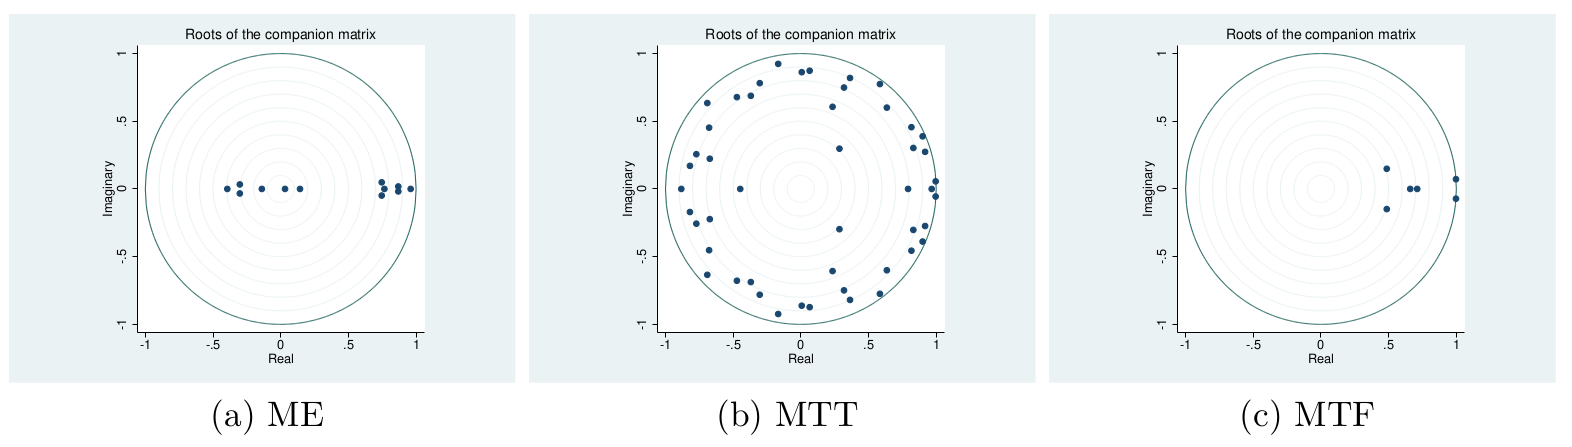
\includegraphics[width=0.99\linewidth]{figure/AUD} 

}

\caption{Eigenvalues of the companion matrix for Australia}\label{fig:FigureE1}
\end{figure}

\begin{figure}[!ht]

{\centering 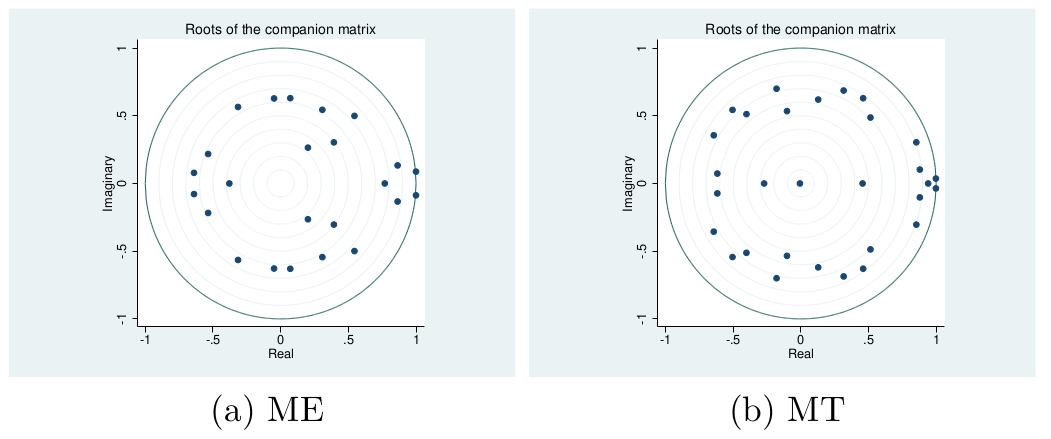
\includegraphics[width=0.66\linewidth]{figure/BRL} 

}

\caption{Eigenvalues of the companion matrix for Brazil}\label{fig:FigureE2}
\end{figure}

\begin{figure}[!ht]

{\centering 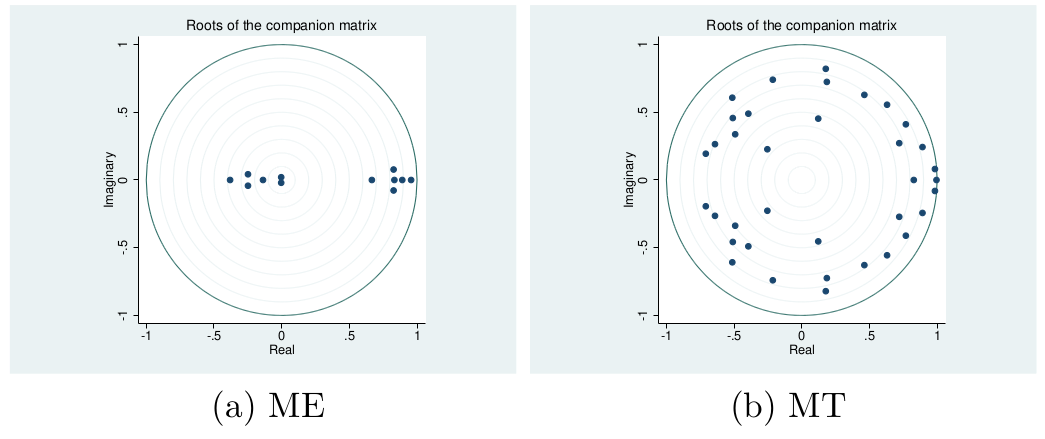
\includegraphics[width=0.66\linewidth]{figure/CAD} 

}

\caption{Eigenvalues of the companion matrix for Canada}\label{fig:FigureE3}
\end{figure}

\clearpage

\begin{figure}[!ht]

{\centering 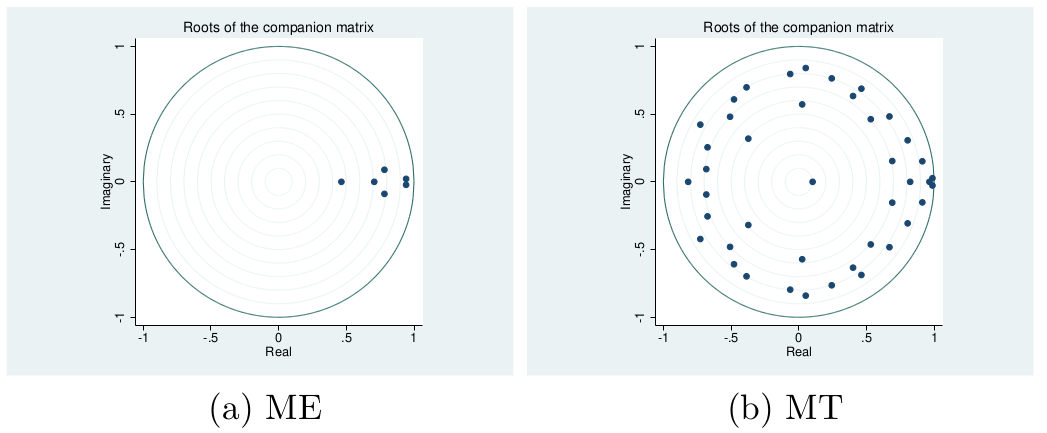
\includegraphics[width=0.66\linewidth]{figure/EUR} 

}

\caption{Eigenvalues of the companion matrix for the Euro area}\label{fig:FigureE4}
\end{figure}

\begin{figure}[!ht]

{\centering 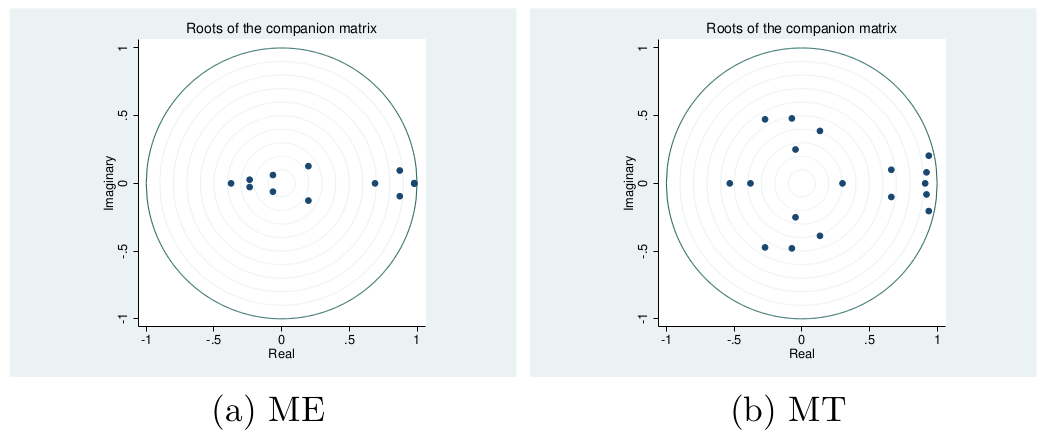
\includegraphics[width=0.66\linewidth]{figure/JPY} 

}

\caption{Eigenvalues of the companion matrix for Japan}\label{fig:FigureE5}
\end{figure}

\begin{figure}[!ht]

{\centering 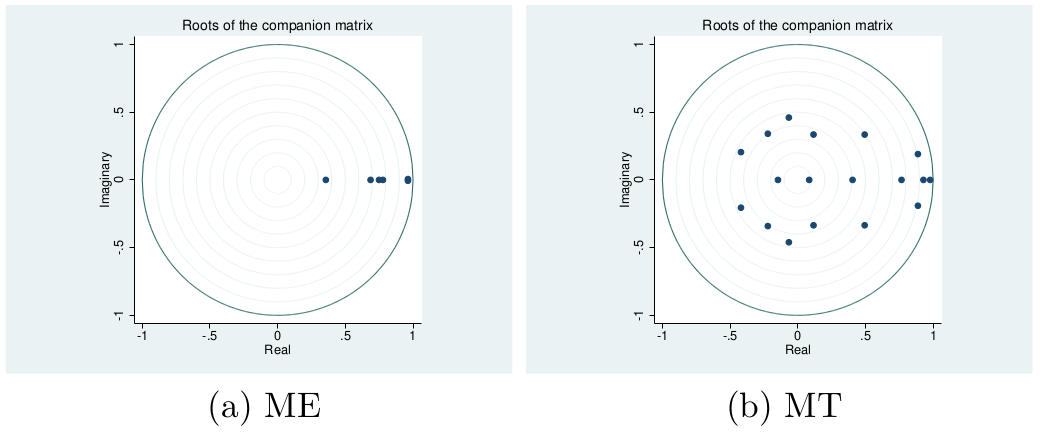
\includegraphics[width=0.66\linewidth]{figure/MXN} 

}

\caption{Eigenvalues of the companion matrix for Mexico}\label{fig:FigureE6}
\end{figure}

\begin{figure}[!ht]

{\centering 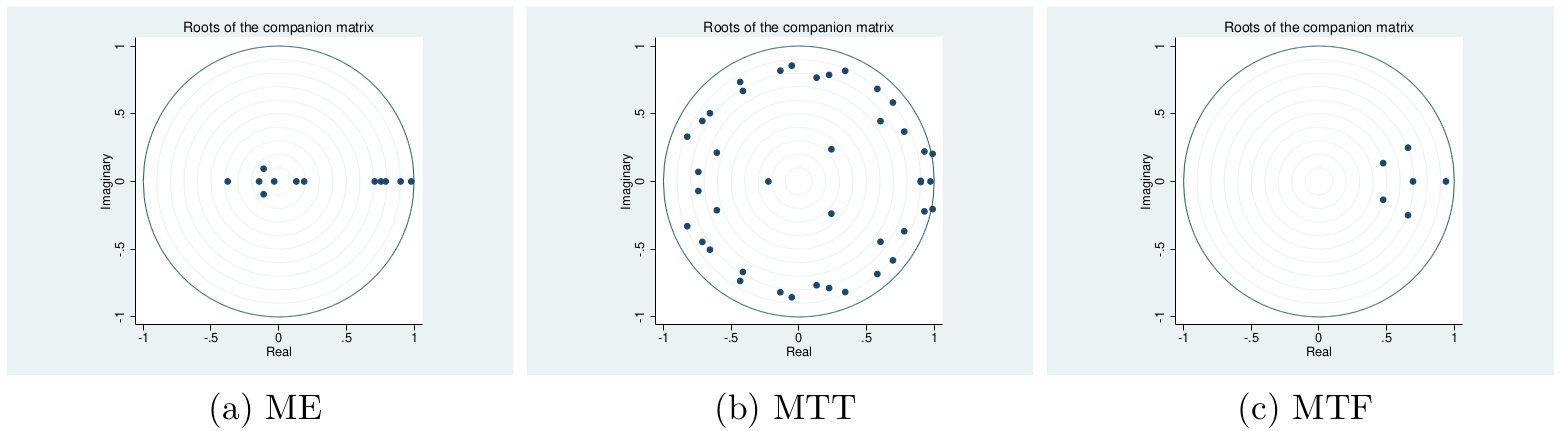
\includegraphics[width=0.99\linewidth]{figure/NZD} 

}

\caption{Eigenvalues of the companion matrix for New Zealand}\label{fig:FigureE7}
\end{figure}

\clearpage

\begin{figure}[!ht]

{\centering 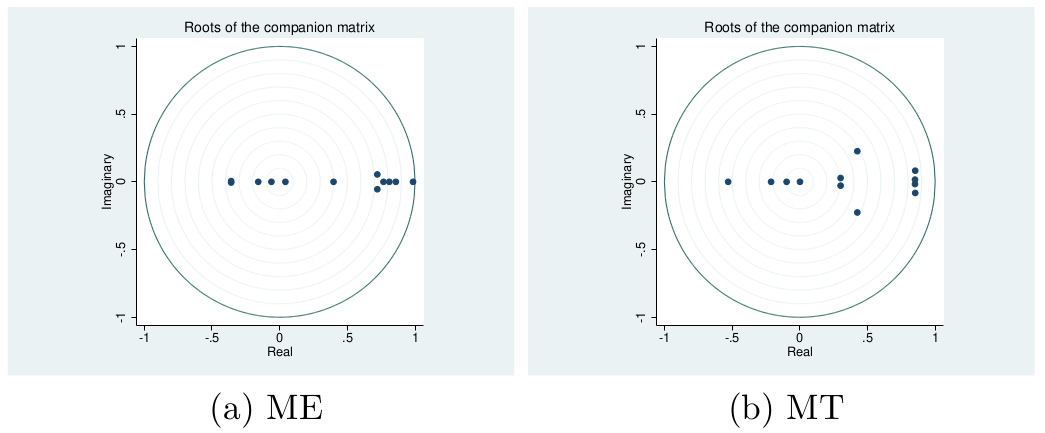
\includegraphics[width=0.66\linewidth]{figure/RBL} 

}

\caption{Eigenvalues of the companion matrix for Russia}\label{fig:FigureE8}
\end{figure}

\begin{figure}[!ht]

{\centering 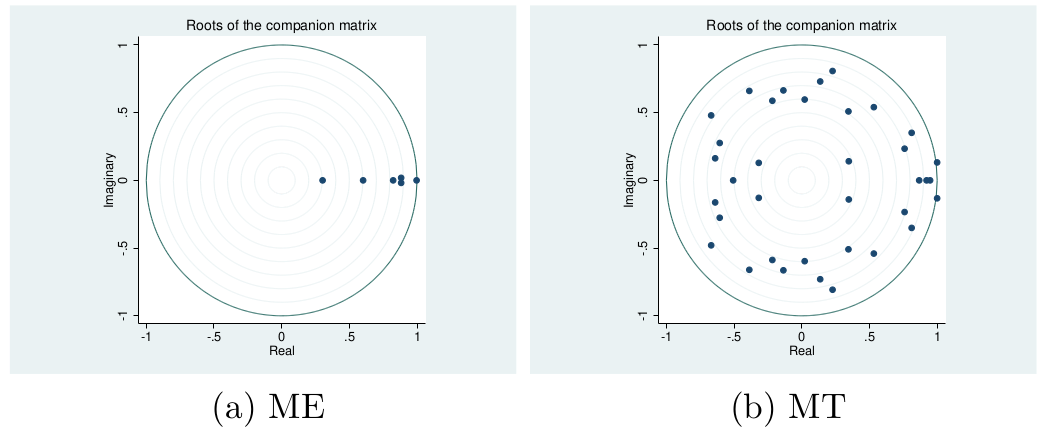
\includegraphics[width=0.66\linewidth]{figure/CHF} 

}

\caption{Eigenvalues of the companion matrix for Switzerland}\label{fig:FigureE9}
\end{figure}

\begin{figure}[!ht]

{\centering 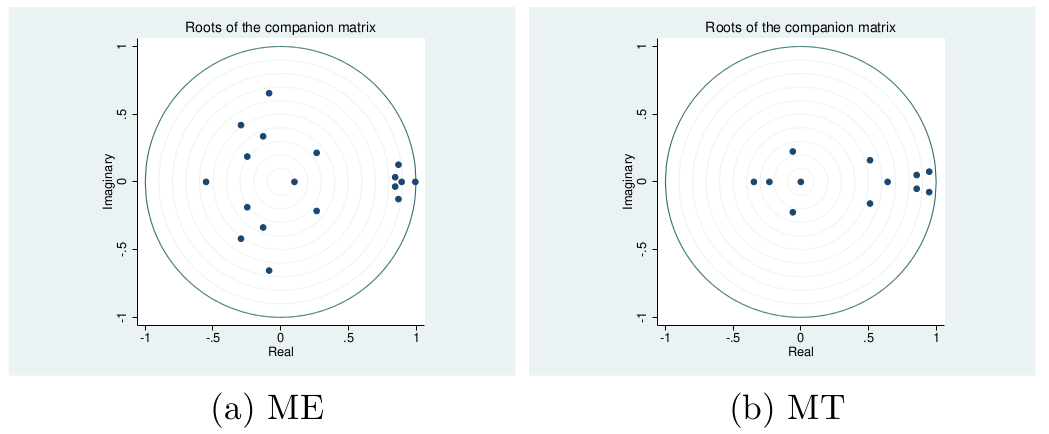
\includegraphics[width=0.66\linewidth]{figure/GBP} 

}

\caption{Eigenvalues of the companion matrix for the United Kingdom}\label{fig:FigureE10}
\end{figure}

\clearpage

\hypertarget{appendixb7}{%
\section{\texorpdfstring{VAR lag length (\(p\)) and exogenous variables}{VAR lag length (p) and exogenous variables}}\label{appendixb7}}

\begin{table}[H]

\caption{\label{tab:TableF1}VAR lag length ($p$) and exogenous variables for Australia}
\centering
\fontsize{10}{12}\selectfont
\begin{tabu} to \linewidth {>{\centering\arraybackslash}p{1cm}>{\centering}X>{\centering\arraybackslash}p{10cm}}
\toprule
Sample & VAR lag length (\(p)\) & Exogenous variables\\
\midrule
ME & 2 & \(TAPER\), \(IRD_{t-3}\), \(ER_{t-3}\), \(SM_{t-3}\), \(SMUS_{t-3}\)\\
MTT & 8 & \(IRD_{t-9}\), \(CT_{t-9}\), \(ER_{t-9}\), \(SMUS_{t-9}\)\\
MTF & 1 & \(IRDF_{t-2}\), \(CTF_{t-2}\), \(SM_{t-2}\), \(SMUS_{t-2}\)\\
\bottomrule
\end{tabu}
\end{table}

\begin{table}[H]

\caption{\label{tab:TableF2}VAR lag length ($p$) and exogenous variables for Brazil}
\centering
\fontsize{10}{12}\selectfont
\begin{tabu} to \linewidth {>{\centering\arraybackslash}p{1cm}>{\centering}X>{\centering\arraybackslash}p{10cm}}
\toprule
Sample & VAR lag length (\(p)\) & Exogenous variables\\
\midrule
ME & 4 & \(CT_{t-5}\), \(IRD_{t-5}\), \(ER_{t-5}\), \(SM_{t-5}\)\\
MT & 5 & \(IRD_{t-6}\), \(VIX_{t-6}\), \(CT_{t-6}\), \(ER_{t-6}\), \(SM_{t-6}\), \(SMUS_{t-6}\)\\
\bottomrule
\end{tabu}
\end{table}

\begin{table}[H]

\caption{\label{tab:TableF3}VAR lag length ($p$) and exogenous variables for Canada}
\centering
\fontsize{10}{12}\selectfont
\begin{tabu} to \linewidth {>{\centering\arraybackslash}p{1cm}>{\centering}X>{\centering\arraybackslash}p{10cm}}
\toprule
Sample & VAR lag length (\(p)\) & Exogenous variables\\
\midrule
ME & 2 & \(TAPER\), \(IRD_{t-4}\), \(ER_{t-4}\), \(SM_{t-4}\), \(SMUS_{t-4}\)\\
MT & 6 & \(IRDF_{t-7}\), \(VIX_{t-7}\), \(CTF_{t-7}\), \(ER_{t-7}\), \(SM_{t-7}\), \(SMUS_{t-7}\)\\
\bottomrule
\end{tabu}
\end{table}

\begin{table}[H]

\caption{\label{tab:TableF4}VAR lag length ($p$) and exogenous variables for the Euro area}
\centering
\fontsize{10}{12}\selectfont
\begin{tabu} to \linewidth {>{\centering\arraybackslash}p{1cm}>{\centering}X>{\centering\arraybackslash}p{10cm}}
\toprule
Sample & VAR lag length (\(p)\) & Exogenous variables\\
\midrule
ME & 1 & \(TAPER\), \(IRD_{t-2}\), \(VIX_{t-2}\), \(CT_{t-2}\), \(ER_{t-2}\), \(SM_{t-2}\), \(SMUS_{t-2}\)\\
MT & 7 & \(IRDF_{t-8}\), \(ER_{t-8}\), \(SMUS_{t-8}\)\\
\bottomrule
\end{tabu}
\end{table}

\begin{table}[H]

\caption{\label{tab:TableF5}VAR lag length ($p$) and exogenous variables for Japan}
\centering
\fontsize{10}{12}\selectfont
\begin{tabu} to \linewidth {>{\centering\arraybackslash}p{1cm}>{\centering}X>{\centering\arraybackslash}p{10cm}}
\toprule
Sample & VAR lag length (\(p)\) & Exogenous variables\\
\midrule
ME & 2 & \(TAPER\), \(IRDF_{t-3}\), \(CTF_{t-3}\), \(ER_{t-3}\), \(SM_{t-3}\), \(SMUS_{t-3}\)\\
MT & 3 & \(IRDF_{t-4}\), \(VIX_{t-4}\), \(CTF_{t-4}\), \(SMUS_{t-4}\)\\
\bottomrule
\end{tabu}
\end{table}

\clearpage

\begin{table}[H]

\caption{\label{tab:TableF6}VAR lag length ($p$) and exogenous variables for Mexico}
\centering
\fontsize{10}{12}\selectfont
\begin{tabu} to \linewidth {>{\centering\arraybackslash}p{1cm}>{\centering}X>{\centering\arraybackslash}p{10cm}}
\toprule
Sample & VAR lag length (\(p)\) & Exogenous variables\\
\midrule
ME & 1 & \(TAPER\), \(CT_{t-2}\), \(SM_{t-2}\), \(SMUS_{t-2}\)\\
MT & 3 & \(VIX_{t-4}\), \(CT_{t-4}\), \(SM_{t-4}\), \(SMUS_{t-4}\)\\
\bottomrule
\end{tabu}
\end{table}

\begin{table}[H]

\caption{\label{tab:TableF7}VAR lag length ($p$) and exogenous variables for New Zealand}
\centering
\fontsize{10}{12}\selectfont
\begin{tabu} to \linewidth {>{\centering\arraybackslash}p{1cm}>{\centering}X>{\centering\arraybackslash}p{10cm}}
\toprule
Sample & VAR lag length (\(p)\) & Exogenous variables\\
\midrule
ME & 2 & \(TAPER\), \(IRD_{t-3}\), \(CT_{t-3}\), \(ER_{t-3}\), \(SM_{t-3}\), \(SMUS_{t-3}\)\\
MTT & 7 & \(IRD_{t-8}\), \(CT_{t-8}\), \(SM_{t-8}\), \(SMUS_{t-8}\)\\
MTF & 1 & \(IRDF_{t-2}\), \(VIX_{t-2}\), \(CTF_{t-2}\), \(ER_{t-2}\), \(SM_{t-2}\), \(SMUS_{t-2}\)\\
\bottomrule
\end{tabu}
\end{table}

\begin{table}[H]

\caption{\label{tab:TableF9}VAR lag length ($p$) and exogenous variables for Switzerland}
\centering
\fontsize{10}{12}\selectfont
\begin{tabu} to \linewidth {>{\centering\arraybackslash}p{1cm}>{\centering}X>{\centering\arraybackslash}p{10cm}}
\toprule
Sample & VAR lag length (\(p)\) & Exogenous variables\\
\midrule
ME & 1 & \(TAPER\), \(IRDF_{t-2}\), \(SM_{t-2}\), \(SMUS_{t-2}\)\\
MT & 6 & \(IRDF_{t-7}\), \(VIX_{t-7}\), \(CTF_{t-7}\), \(SMUS_{t-7}\)\\
\bottomrule
\end{tabu}
\end{table}

\begin{table}[H]

\caption{\label{tab:TableF10}VAR lag length ($p$) and exogenous variables for the United Kingdom}
\centering
\fontsize{10}{12}\selectfont
\begin{tabu} to \linewidth {>{\centering\arraybackslash}p{1cm}>{\centering}X>{\centering\arraybackslash}p{10cm}}
\toprule
Sample & VAR lag length (\(p)\) & Exogenous variables\\
\midrule
ME & 3 & \(TAPER\), \(ER_{t-4}\), \(SM_{t-4}\), \(SMUS_{t-4}\)\\
MT & 2 & \(IRDF_{t-3}\), \(VIX_{t-3}\), \(CTF_{t-3}\), \(ER_{t-7}\), \(SMUS_{t-7}\)\\
\bottomrule
\end{tabu}
\end{table}

\clearpage

\hypertarget{appendixb8}{%
\section{Granger causality tests}\label{appendixb8}}

\begin{table}[H]

\caption{\label{tab:Granger}Results from the Granger causality tests for target currencies, during ME}
\centering
\resizebox{\linewidth}{!}{
\begin{tabular}[t]{lcccccccc}
\toprule
Direction & Australia & Brazil & Canada & Euro area & Mexico & New Zealand & Russia & United Kingdom\\
\midrule
$ER$$\rightarrow$$CT$ & 0.0690 & 0.0138 & 0.3964 & 0.0018 & 0.4464 & 0.0075 & 0.8960 & 0.0001\\
$IRD$$\rightarrow$$CT$ & 0.3713 & 0.8548 & 0.9922 & 0.0648 & 0.1380 & 0.8657 & 0.9999 & 0.4233\\
$VIX$$\rightarrow$$CT$ & 0.0440 & 0.3617 & 0.7171 & 0.9997 & 0.0284 & 0.4763 & 0.2621 & 0.7454\\
$SM$$\rightarrow$$CT$ & 0.9281 & 0.0072 & 0.7768 & 0.7238 & 0.9543 & 0.6224 & 0.8321 & 0.1410\\
$SMUS$$\rightarrow$$CT$ & 0.7600 & 0.8281 & 0.7653 & 0.5735 & 0.7690 & 0.6691 & 0.8158 & 0.5969\\
All$\rightarrow$$CT$ & 0.0237 & 0.0136 & 0.6446 & 0.0193 & 0.0841 & 0.1286 & 0.9648 & 0.0008\\
\addlinespace
$CT$$\rightarrow$$ER$ & 0.0107 & 0.7520 & 0.6495 & 0.4133 & 0.8426 & 0.2216 & 0.6354 & 0.3816\\
$IRD$$\rightarrow$$ER$ & 0.5100 & 0.1664 & 0.8142 & 0.2514 & 0.3714 & 0.2302 & 0.0000 & 0.0075\\
$VIX$$\rightarrow$$ER$ & 0.7462 & 0.1922 & 0.0619 & 0.0202 & 0.2137 & 0.8917 & 0.6561 & 0.3815\\
$SM$$\rightarrow$$ER$ & 0.3406 & 0.6495 & 0.5896 & 0.1491 & 0.8115 & 0.9855 & 0.5881 & 0.0429\\
$SMUS$$\rightarrow$$ER$ & 0.9184 & 0.5652 & 0.0688 & 0.5702 & 0.3590 & 0.5476 & 0.2198 & 0.1691\\
All$\rightarrow$$ER$ & 0.1000 & 0.4998 & 0.3309 & 0.1356 & 0.5503 & 0.6470 & 0.0000 & 0.0069\\
\addlinespace
$CT$$\rightarrow$$IRD$ & 0.0177 & 0.3516 & 0.1778 & 0.4627 & 0.8025 & 0.9520 & 0.9972 & 0.3306\\
$ER$$\rightarrow$$IRD$ & 0.1810 & 0.0021 & 0.0344 & 0.4386 & 0.9978 & 0.0181 & 0.0000 & 0.0005\\
$VIX$$\rightarrow$$IRD$ & 0.8757 & 0.0089 & 0.1354 & 0.5114 & 0.2316 & 0.0000 & 0.6136 & 0.0000\\
$SM$$\rightarrow$$IRD$ & 0.0647 & 0.0230 & 0.1697 & 0.8884 & 0.8220 & 0.9084 & 0.7946 & 0.0014\\
$SMUS$$\rightarrow$$IRD$ & 0.7580 & 0.1194 & 0.6713 & 0.8272 & 0.4466 & 0.6566 & 0.5767 & 0.8311\\
All$\rightarrow$$IRD$ & 0.0579 & 0.0003 & 0.0668 & 0.9528 & 0.6783 & 0.0002 & 0.0131 & 0.0000\\
\addlinespace
$CT$$\rightarrow$$VIX$ & 0.5771 & 0.4374 & 0.8560 & 0.8216 & 0.6449 & 0.8596 & 0.5584 & 0.6353\\
$ER$$\rightarrow$$VIX$ & 0.4843 & 0.1055 & 0.3234 & 0.8271 & 0.8306 & 0.1698 & 0.6387 & 0.2068\\
$IRD$$\rightarrow$$VIX$ & 0.6797 & 0.3570 & 0.0568 & 0.0915 & 0.0016 & 0.4442 & 0.1573 & 0.4209\\
$SM$$\rightarrow$$VIX$ & 0.1345 & 0.7741 & 0.7185 & 0.3863 & 0.4057 & 0.6638 & 0.2961 & 0.1859\\
$SMUS$$\rightarrow$$VIX$ & 0.3430 & 0.3479 & 0.9260 & 0.9076 & 0.0986 & 0.5921 & 0.8950 & 0.8850\\
All$\rightarrow$$VIX$ & 0.4988 & 0.3199 & 0.4170 & 0.5686 & 0.0212 & 0.7202 & 0.6689 & 0.3577\\
\addlinespace
$CT$$\rightarrow$$SM$ & 0.1746 & 0.5165 & 0.6145 & 0.6277 & 0.8965 & 0.8159 & 0.9956 & 0.4886\\
$ER$$\rightarrow$$SM$ & 0.9063 & 0.2800 & 0.7281 & 0.8364 & 0.4455 & 0.0962 & 0.9784 & 0.0052\\
$IRD$$\rightarrow$$SM$ & 0.8038 & 0.3315 & 0.7394 & 0.9278 & 0.0046 & 0.9015 & 0.5747 & 0.0719\\
$VIX$$\rightarrow$$SM$ & 0.0032 & 0.8471 & 0.4429 & 0.8781 & 0.7541 & 0.8175 & 0.5677 & 0.3244\\
$SMUS$$\rightarrow$$SM$ & 0.8038 & 0.3955 & 0.6337 & 0.4060 & 0.3939 & 0.0320 & 0.6376 & 0.7423\\
All$\rightarrow$$SM$ & 0.0042 & 0.4319 & 0.7926 & 0.9673 & 0.0492 & 0.3063 & 0.9409 & 0.0388\\
\addlinespace
$CT$$\rightarrow$$SMUS$ & 0.3218 & 0.7105 & 0.4273 & 0.3054 & 0.1188 & 0.9883 & 0.5931 & 0.7541\\
$ER$$\rightarrow$$SMUS$ & 0.5864 & 0.5104 & 0.3952 & 0.2117 & 0.0023 & 0.4290 & 0.9747 & 0.8213\\
$IRD$$\rightarrow$$SMUS$ & 0.9055 & 0.0282 & 0.8518 & 0.9245 & 0.1131 & 0.7727 & 0.6114 & 0.7082\\
$VIX$$\rightarrow$$SMUS$ & 0.5987 & 0.5448 & 0.0220 & 0.7769 & 0.5946 & 0.1350 & 0.0436 & 0.9570\\
$SM$$\rightarrow$$SMUS$ & 0.0568 & 0.1624 & 0.1260 & 0.3052 & 0.0341 & 0.2913 & 0.5814 & 0.0694\\
All$\rightarrow$$SMUS$ & 0.1241 & 0.1868 & 0.0392 & 0.6960 & 0.0025 & 0.3311 & 0.3779 & 0.1112\\
\bottomrule
\end{tabular}}
\end{table}

\clearpage

\begin{table}[H]

\caption{\label{tab:Granger2}Results from the Granger causality tests for funding currencies, during ME}
\centering
\fontsize{10}{12}\selectfont
\begin{tabular}[t]{lcc}
\toprule
Direction & Japan & Switzerland\\
\midrule
$ER$$\rightarrow$$CTF$ & 0.0001 & 0.0315\\
$IRDF$$\rightarrow$$CTF$ & 0.9882 & 0.2420\\
$VIX$$\rightarrow$$CTF$ & 0.0538 & 0.7194\\
$SM$$\rightarrow$$CTF$ & 0.7254 & 0.1945\\
$SMUS$$\rightarrow$$CTF$ & 0.8043 & 0.3151\\
All$\rightarrow$$CTF$ & 0.0031 & 0.1662\\
\addlinespace
$CTF$$\rightarrow$$ER$ & 0.0219 & 0.2932\\
$IRDF$$\rightarrow$$ER$ & 0.3885 & 0.2241\\
$VIX$$\rightarrow$$ER$ & 0.9978 & 0.1049\\
$SM$$\rightarrow$$ER$ & 0.0946 & 0.4576\\
$SMUS$$\rightarrow$$ER$ & 0.5895 & 0.9085\\
All$\rightarrow$$ER$ & 0.1182 & 0.1320\\
\addlinespace
$CTF$$\rightarrow$$IRDF$ & 0.7318 & 0.0559\\
$ER$$\rightarrow$$IRDF$ & 0.1483 & 0.4630\\
$VIX$$\rightarrow$$IRDF$ & 0.9897 & 0.0004\\
$SM$$\rightarrow$$IRDF$ & 0.9955 & 0.1588\\
$SMUS$$\rightarrow$$IRDF$ & 0.6466 & 0.7544\\
All$\rightarrow$$IRDF$ & 0.8856 & 0.0022\\
\addlinespace
$CTF$$\rightarrow$$VIX$ & 0.9337 & 0.8266\\
$ER$$\rightarrow$$VIX$ & 0.0801 & 0.1711\\
$IRDF$$\rightarrow$$VIX$ & 0.5887 & 0.9716\\
$SM$$\rightarrow$$VIX$ & 0.9871 & 0.9410\\
$SMUS$$\rightarrow$$VIX$ & 0.5406 & 0.4742\\
All$\rightarrow$$VIX$ & 0.5622 & 0.7994\\
\addlinespace
$CTF$$\rightarrow$$SM$ & 0.4511 & 0.0362\\
$ER$$\rightarrow$$SM$ & 0.0089 & 0.0017\\
$IRDF$$\rightarrow$$SM$ & 0.9784 & 0.5966\\
$VIX$$\rightarrow$$SM$ & 0.0009 & 0.0002\\
$SMUS$$\rightarrow$$SM$ & 0.5790 & 0.0976\\
All$\rightarrow$$SM$ & 0.0009 & 0.0005\\
\addlinespace
$CTF$$\rightarrow$$SMUS$ & 0.4869 & 0.0052\\
$ER$$\rightarrow$$SMUS$ & 0.3002 & 0.0000\\
$IRDF$$\rightarrow$$SMUS$ & 0.8591 & 0.3359\\
$VIX$$\rightarrow$$SMUS$ & 0.0026 & 0.1155\\
$SM$$\rightarrow$$SMUS$ & 0.8317 & 0.0260\\
All$\rightarrow$$SMUS$ & 0.0383 & 0.0000\\
\bottomrule
\end{tabular}
\end{table}

\begin{table}[H]

\caption{\label{tab:Granger3}Results from the Granger causality tests for target currencies, during MT}
\centering
\fontsize{10}{12}\selectfont
\begin{tabular}[t]{lccccc}
\toprule
Direction & Australia* & Brazil & Mexico & New Zealand* & Russia\\
\midrule
$ER$$\rightarrow$$CT$ & 0.0036 & 0.0938 & 0.0075 & 0.4363 & 0.5043\\
$IRD$$\rightarrow$$CT$ & 0.0783 & 0.0429 & 0.0142 & 0.7138 & 0.2712\\
$VIX$$\rightarrow$$CT$ & 0.5150 & 0.7410 & 0.4638 & 0.1302 & 0.0001\\
$SM$$\rightarrow$$CT$ & 0.5115 & 0.4735 & 0.8785 & 0.6977 & 0.4899\\
$SMUS$$\rightarrow$$CT$ & 0.0144 & 0.6990 & 0.6085 & 0.1170 & 0.2214\\
All$\rightarrow$$CT$ & 0.0133 & 0.2299 & 0.1219 & 0.1943 & 0.0002\\
\addlinespace
$CT$$\rightarrow$$ER$ & 0.1550 & 0.4449 & 0.5304 & 0.2292 & 0.4339\\
$IRD$$\rightarrow$$ER$ & 0.0008 & 0.5264 & 0.6614 & 0.8929 & 0.2792\\
$VIX$$\rightarrow$$ER$ & 0.7183 & 0.1250 & 0.8208 & 0.8863 & 0.6138\\
$SM$$\rightarrow$$ER$ & 0.0844 & 0.5766 & 0.0808 & 0.0274 & 0.0012\\
$SMUS$$\rightarrow$$ER$ & 0.8726 & 0.3018 & 0.4848 & 0.6808 & 0.7780\\
All$\rightarrow$$ER$ & 0.0261 & 0.2932 & 0.6350 & 0.6806 & 0.0042\\
\addlinespace
$CT$$\rightarrow$$IRD$ & 0.0080 & 0.0340 & 0.3040 & 0.4252 & 0.6712\\
$ER$$\rightarrow$$IRD$ & 0.0128 & 0.7682 & 0.0001 & 0.0002 & 0.7991\\
$VIX$$\rightarrow$$IRD$ & 0.0108 & 0.8955 & 0.0131 & 0.0032 & 0.0630\\
$SM$$\rightarrow$$IRD$ & 0.5254 & 0.5157 & 0.5039 & 0.0001 & 0.9392\\
$SMUS$$\rightarrow$$IRD$ & 0.1296 & 0.9876 & 0.2069 & 0.0022 & 0.2594\\
All$\rightarrow$$IRD$ & 0.0016 & 0.7168 & 0.0023 & 0.0001 & 0.6069\\
\addlinespace
$CT$$\rightarrow$$VIX$ & 0.0197 & 0.1902 & 0.8782 & 0.7429 & 0.9249\\
$ER$$\rightarrow$$VIX$ & 0.3473 & 0.0017 & 0.5916 & 0.0782 & 0.9495\\
$IRD$$\rightarrow$$VIX$ & 0.1943 & 0.1462 & 0.0386 & 0.0004 & 0.1342\\
$SM$$\rightarrow$$VIX$ & 0.1048 & 0.2057 & 0.9443 & 0.0514 & 0.5234\\
$SMUS$$\rightarrow$$VIX$ & 0.0850 & 0.1873 & 0.0545 & 0.0351 & 0.2167\\
All$\rightarrow$$VIX$ & 0.0071 & 0.0046 & 0.2489 & 0.0016 & 0.6356\\
\addlinespace
$CT$$\rightarrow$$SM$ & 0.2061 & 0.6003 & 0.6589 & 0.9668 & 0.9934\\
$ER$$\rightarrow$$SM$ & 0.0136 & 0.0012 & 0.2029 & 0.1683 & 0.9409\\
$IRD$$\rightarrow$$SM$ & 0.1993 & 0.8110 & 0.3157 & 0.0012 & 0.7365\\
$VIX$$\rightarrow$$SM$ & 0.2292 & 0.6518 & 0.3163 & 0.5152 & 0.8777\\
$SMUS$$\rightarrow$$SM$ & 0.0047 & 0.0002 & 0.2104 & 0.1077 & 0.4756\\
All$\rightarrow$$SM$ & 0.0260 & 0.0001 & 0.0542 & 0.0043 & 0.5405\\
\addlinespace
$CT$$\rightarrow$$SMUS$ & 0.2613 & 0.8902 & 0.5674 & 0.2531 & 0.8246\\
$ER$$\rightarrow$$SMUS$ & 0.5016 & 0.1339 & 0.6359 & 0.0229 & 0.3582\\
$IRD$$\rightarrow$$SMUS$ & 0.0272 & 0.7087 & 0.0324 & 0.0022 & 0.0898\\
$VIX$$\rightarrow$$SMUS$ & 0.1371 & 0.1346 & 0.1738 & 0.2567 & 0.8957\\
$SM$$\rightarrow$$SMUS$ & 0.1035 & 0.2456 & 0.9385 & 0.2282 & 0.1598\\
All$\rightarrow$$SMUS$ & 0.0178 & 0.4218 & 0.2107 & 0.0027 & 0.2435\\
\bottomrule
\multicolumn{6}{l}{\rule{0pt}{1em}\textit{*: } MTT sample. }\\
\end{tabular}
\end{table}

\begin{table}[H]

\caption{\label{tab:Granger4}Results from the Granger causality tests for funding currencies, during MT}
\centering
\resizebox{\linewidth}{!}{
\begin{tabular}[t]{lccccccc}
\toprule
Direction & Australia* & Canada & Euro area & Japan & New Zealand* & Switzerland & United Kingdom\\
\midrule
$ER$$\rightarrow$$CTF$ & 0.0323 & 0.6226 & 0.0759 & 0.0412 & 0.0134 & 0.0295 & 0.0008\\
$IRDF$$\rightarrow$$CTF$ & 0.1012 & 0.6228 & 0.0279 & 0.5194 & 0.1053 & 0.0913 & 0.9577\\
$VIX$$\rightarrow$$CTF$ & 0.8550 & 0.4557 & 0.7845 & 0.3446 & 0.8448 & 0.1613 & 0.3457\\
$SM$$\rightarrow$$CTF$ & 0.0715 & 0.7414 & 0.3672 & 0.0001 & 0.2399 & 0.3978 & 0.5971\\
$SMUS$$\rightarrow$$CTF$ & 0.1909 & 0.1372 & 0.6791 & 0.1677 & 0.7215 & 0.0066 & 0.8893\\
All$\rightarrow$$CTF$ & 0.0656 & 0.3900 & 0.1033 & 0.0000 & 0.0718 & 0.0052 & 0.0411\\
\addlinespace
$CTF$$\rightarrow$$ER$ & 0.1040 & 0.0185 & 0.0994 & 0.8205 & 0.2880 & 0.6266 & 0.0972\\
$IRDF$$\rightarrow$$ER$ & 0.0007 & 0.0215 & 0.7783 & 0.9660 & 0.1773 & 0.9764 & 0.7530\\
$VIX$$\rightarrow$$ER$ & 0.6237 & 0.0005 & 0.7966 & 0.6043 & 0.6098 & 0.9476 & 0.4816\\
$SM$$\rightarrow$$ER$ & 0.7962 & 0.0010 & 0.1113 & 0.4580 & 0.4542 & 0.2225 & 0.3431\\
$SMUS$$\rightarrow$$ER$ & 0.6046 & 0.0000 & 0.7992 & 0.6584 & 0.7671 & 0.6352 & 0.3323\\
All$\rightarrow$$ER$ & 0.0205 & 0.0000 & 0.1842 & 0.8730 & 0.4242 & 0.7470 & 0.3646\\
\addlinespace
$CTF$$\rightarrow$$IRDF$ & 0.3168 & 0.4607 & 0.4433 & 0.3287 & 0.2086 & 0.1635 & 0.5902\\
$ER$$\rightarrow$$IRDF$ & 0.4755 & 0.6922 & 0.2328 & 0.2655 & 0.2418 & 0.1290 & 0.7120\\
$VIX$$\rightarrow$$IRDF$ & 0.6534 & 0.0000 & 0.0025 & 0.4208 & 0.0514 & 0.2361 & 0.3303\\
$SM$$\rightarrow$$IRDF$ & 0.7391 & 0.3858 & 0.5049 & 0.8955 & 0.3692 & 0.6637 & 0.7997\\
$SMUS$$\rightarrow$$IRDF$ & 0.6759 & 0.9172 & 0.8999 & 0.5934 & 0.5511 & 0.6857 & 0.5534\\
All$\rightarrow$$IRDF$ & 0.7488 & 0.0000 & 0.0342 & 0.6732 & 0.0242 & 0.3141 & 0.9149\\
\addlinespace
$CTF$$\rightarrow$$VIX$ & 0.1866 & 0.1501 & 0.4112 & 0.7560 & 0.5621 & 0.0079 & 0.0231\\
$ER$$\rightarrow$$VIX$ & 0.6672 & 0.2507 & 0.7847 & 0.5495 & 0.9307 & 0.1620 & 0.4956\\
$IRDF$$\rightarrow$$VIX$ & 0.8150 & 0.9923 & 0.2786 & 0.8094 & 0.6795 & 0.0239 & 0.5241\\
$SM$$\rightarrow$$VIX$ & 0.5453 & 0.7634 & 0.2351 & 0.0946 & 0.3207 & 0.0070 & 0.8016\\
$SMUS$$\rightarrow$$VIX$ & 0.9954 & 0.0747 & 0.7538 & 0.0451 & 0.7772 & 0.0136 & 0.2962\\
All$\rightarrow$$VIX$ & 0.8620 & 0.0584 & 0.2352 & 0.1677 & 0.8905 & 0.0013 & 0.2538\\
\addlinespace
$CTF$$\rightarrow$$SM$ & 0.2746 & 0.1350 & 0.0916 & 0.1237 & 0.6962 & 0.5049 & 0.8341\\
$ER$$\rightarrow$$SM$ & 0.8911 & 0.0120 & 0.3873 & 0.2035 & 0.6838 & 0.4888 & 0.7305\\
$IRDF$$\rightarrow$$SM$ & 0.5978 & 0.1451 & 0.3450 & 0.1125 & 0.8307 & 0.0272 & 0.0002\\
$VIX$$\rightarrow$$SM$ & 0.4580 & 0.0289 & 0.9454 & 0.1237 & 0.7968 & 0.1481 & 0.0423\\
$SMUS$$\rightarrow$$SM$ & 0.3249 & 0.0676 & 0.0003 & 0.8417 & 0.8955 & 0.1642 & 0.1576\\
All$\rightarrow$$SM$ & 0.7069 & 0.0052 & 0.0012 & 0.0005 & 0.9361 & 0.0176 & 0.0002\\
\addlinespace
$CTF$$\rightarrow$$SMUS$ & 0.1801 & 0.0012 & 0.0162 & 0.7724 & 0.2835 & 0.0000 & 0.0593\\
$ER$$\rightarrow$$SMUS$ & 0.8683 & 0.1123 & 0.1087 & 0.0618 & 0.6650 & 0.0418 & 0.5745\\
$IRDF$$\rightarrow$$SMUS$ & 0.5462 & 0.1967 & 0.0314 & 0.5865 & 0.5298 & 0.0003 & 0.3604\\
$VIX$$\rightarrow$$SMUS$ & 0.8036 & 0.4923 & 0.5921 & 0.1685 & 0.3194 & 0.0740 & 0.6171\\
$SM$$\rightarrow$$SMUS$ & 0.7455 & 0.1239 & 0.0521 & 0.1285 & 0.2429 & 0.0049 & 0.7697\\
All$\rightarrow$$SMUS$ & 0.6186 & 0.0001 & 0.0133 & 0.1653 & 0.5594 & 0.0000 & 0.3411\\
\bottomrule
\multicolumn{8}{l}{\rule{0pt}{1em}\textit{*: } MTF sample. }\\
\end{tabular}}
\end{table}

\hypertarget{appendixc}{%
\chapter{Supplemental Material for Chapter 3}\label{appendixc}}

\hypertarget{appendixc1}{%
\section{Descriptive statistics and actual evolution of the variables}\label{appendixc1}}

Table \ref{tab:TableA1} shows the descriptive statistics of our data, while the actual evolution is presented in Figure \ref{fig:FigureA1}.

\begin{table}[H]

\caption{\label{tab:TableA1}Descriptive statistics}
\centering
\fontsize{10}{12}\selectfont
\begin{tabular}[t]{lccccccc}
\toprule
  & Obs. & Mean & Std. Dev. & Variance & Skewness & Min. & Max.\\
\midrule
$CT\textsubscript{USD}$ & 310 & 0.06 & 0.35 & 0.12 & -0.01 & -0.73 & 0.83\\
$CT\textsubscript{EUR}$ & 310 & 0.06 & 0.34 & 0.11 & -0.42 & -0.67 & 0.66\\
$CT\textsubscript{JPY}$ & 310 & 0.04 & 0.32 & 0.10 & -0.42 & -0.64 & 0.65\\
$CT\textsubscript{GBP}$ & 310 & 0.05 & 0.32 & 0.10 & -0.53 & -0.67 & 0.66\\
\addlinespace
$IRD\textsubscript{USD}$ & 310 & -1.53 & 0.82 & 0.68 & -0.37 & -2.98 & -0.07\\
$IRD\textsubscript{EUR}$ & 310 & -0.13 & 0.17 & 0.03 & -0.99 & -0.59 & 0.17\\
$IRD\textsubscript{JPY}$ & 310 & -0.49 & 0.10 & 0.01 & 0.65 & -0.77 & 0.00\\
$IRD\textsubscript{GBP}$ & 310 & -0.96 & 0.24 & 0.06 & 0.44 & -1.43 & -0.42\\
\addlinespace
$ER\textsubscript{USD}$ & 310 & -0.03 & 0.03 & 0.00 & -0.90 & -0.14 & 0.03\\
$ER\textsubscript{EUR}$ & 310 & 0.10 & 0.04 & 0.00 & 0.44 & 0.01 & 0.18\\
$ER\textsubscript{JPY}$ & 310 & 4.74 & 0.05 & 0.00 & 1.01 & 4.64 & 4.91\\
$ER\textsubscript{GBP}$ & 310 & 0.27 & 0.07 & 0.01 & 0.63 & 0.14 & 0.44\\
\addlinespace
$FSM\textsubscript{USD}$ & 310 & 7.83 & 0.17 & 0.03 & 0.08 & 7.52 & 8.20\\
$FSM\textsubscript{EUR}$ & 310 & 6.88 & 0.09 & 0.01 & -0.25 & 6.65 & 7.07\\
$FSM\textsubscript{JPY}$ & 310 & 9.92 & 0.12 & 0.01 & -0.42 & 9.64 & 10.17\\
$FSM\textsubscript{GBP}$ & 310 & 8.84 & 0.09 & 0.01 & -0.65 & 8.57 & 8.97\\
\addlinespace
$SM$ & 310 & 9.11 & 0.08 & 0.01 & 0.14 & 8.93 & 9.32\\
$VIX$ & 310 & 2.79 & 0.36 & 0.13 & 1.13 & 2.24 & 4.33\\
\bottomrule
\end{tabular}
\end{table}

\clearpage

\begin{figure}[!ht]

{\centering \includegraphics[width=0.99\columnwidth]{figure/PLOTALL-larger} 

}

\caption[Actual evolution of the variables]{Actual evolution of the variables \newline \scriptsize \textit{Notes:} The shaded areas correspond to the time dummies: (USD) $USME$, monetary easing in the U.S. (8/6/2019-11/24/2020), (EUR) $ZLBEUR$, policy interest rate equal to zero for the Euro (3/22/2016-11/24/2020), (JPY) $NIJPY$, negative interest rate policy in Japan (9/27/2016-11/24/2020), and (GBP) $BREXIT$, effective date of the withdrawal of the United Kingdom from the European Union (2/4/2020-11/24/2020).}\label{fig:FigureA1}
\end{figure}

\clearpage

\hypertarget{appendixc2}{%
\section{Unit root tests}\label{appendixc2}}

We opt for the \textcite{clemente1998} test with the innovational outlier (IO) model. This test with two structural breaks and unknown breakpoints fits our data well with means shifting gradually. Table \ref{tab:TableB1} presents the results of the unit root tests.



\begin{table}[!ht]

\caption{\label{tab:TableB1}Clemente-Montañés-Reyes unit-root tests, innovational outlier (IO) model}
\centering
\begin{threeparttable}
\begin{tabular}[t]{l>{\centering\arraybackslash}p{1,5cm}>{\centering\arraybackslash}p{1,5cm}>{\centering\arraybackslash}p{1,5cm}>{\centering\arraybackslash}p{1,5cm}>{\centering\arraybackslash}p{1,5cm}lc}
\toprule
\multicolumn{1}{c}{ } & \multicolumn{2}{c}{Levels} & \multicolumn{2}{c}{First-differences} & \multicolumn{2}{c}{Second-differences} & \multicolumn{1}{c}{ } \\
\cmidrule(l{3pt}r{3pt}){2-3} \cmidrule(l{3pt}r{3pt}){4-5} \cmidrule(l{3pt}r{3pt}){6-7}
  & $(\rho - 1)$ & t-stat & $(\rho - 1)$ & t-stat & $(\rho - 1)$ & t-stat & I($d$)\\
\midrule
$CT\textsubscript{USD}$ & -0.1454 & -4.7877 & -1.4772 & -5.5578 &  &  & I(1)\\
$CT\textsubscript{EUR}$ & -0.1446 & -4.7119 & -1.2112 & -23.9101 &  &  & I(1)\\
$CT\textsubscript{JPY}$ & -0.1722 & -4.6392 & -2.0116 & -7.1027 &  &  & I(1)\\
$CT\textsubscript{GBP}$ & -0.171 & -3.8966 & -2.3402 & -8.0398 &  &  & I(1)\\
$ER\textsubscript{USD}$ & -0.176 & -4.6953 & -1.7483 & -10.2286 &  &  & I(1)\\
$ER\textsubscript{EUR}$ & -0.0932 & -4.6791 & -0.911 & -4.8282 & -6.4545 & -8.6273 & I(2)\\
$ER\textsubscript{JPY}$ & -0.1151 & -4.2935 & -1.6916 & -10.8537 &  &  & I(1)\\
$ER\textsubscript{GBP}$ & -0.1701 & -5.9869 &  &  &  &  & I(0)\\
$IRD\textsubscript{USD}$ & -0.063 & -5.5146 &  &  &  &  & I(0)\\
$IRD\textsubscript{EUR}$ & -0.2084 & -7.3311 &  &  &  &  & I(0)\\
$IRD\textsubscript{JPY}$ & -0.1981 & -8.4496 &  &  &  &  & I(0)\\
$IRD\textsubscript{GBP}$ & -0.1263 & -7.0012 &  &  &  &  & I(0)\\
$FSM\textsubscript{USD}$ & -0.0563 & -3.3056 & -1.3167 & -8.5508 &  &  & I(1)\\
$FSM\textsubscript{EUR}$ & -0.1522 & -5.0798 & -1.2607 & -17.5674 &  &  & I(1)\\
$FSM\textsubscript{JPY}$ & -0.0818 & -4.0181 & -1.5405 & -7.3962 &  &  & I(1)\\
$FSM\textsubscript{GBP}$ & -0.1592 & -6.4903 &  &  &  &  & I(0)\\
$VIX$ & -0.1983 & -5.0078 & -1.7286 & -10.846 &  &  & I(1)\\
$SM$ & -0.0892 & -3.8995 & -1.5127 & -11.4007 &  &  & I(1)\\
\bottomrule
\end{tabular}
\begin{tablenotes}[para]
\item \textit{\footnotesize{Note: }} 
\item \footnotesize{Test for stationarity in the presence of a double structural break in the series, which considers the null hypothesis that $(\rho - 1)$ is different from zero. Critical t-stat value (T $=$ 100, $\infty$, 5\% sig.) = -5.19 \autocite[Table 1]{clemente1998}.}
\end{tablenotes}
\end{threeparttable}
\end{table}

\clearpage

\hypertarget{appendixc3}{%
\section{Model specification}\label{appendixc3}}

Variables that are not stationary in levels must be added as lagged exogenous variables in the SVAR model. The number of lags of these variables is specified by \(d\) plus \(p\). In doing so, we are proceeding with a modified Wald test (MWald test). Therefore, as asserted by \textcite[\text{p.} 226]{toda1995}, ``it is clearly desirable to have a testing procedure which is robust to the integration and cointegration properties of the process so as to avoid the possible pretest biases.''

In order to obtain the lag length \(p\) of the SVAR model, the Lagrange-multiplier (LM) test for residual autocorrelation is used (see Table \ref{tab:TableC1}). The correct lag order cannot be achieved by merely verifying the optimal lag length. Moreover, the lag order \(p\) must not have autocorrelated residuals. Nevertheless, small VAR dimensions are preferable \autocite{toda1995,dolado1996}.

\begin{table}[!ht]

\caption{\label{tab:TableC1}Lagrange-multiplier (LM) test for residual autocorrelation, p-values}
\centering
\begin{threeparttable}
\begin{tabular}[t]{c>{\centering\arraybackslash}p{2,2cm}>{\centering\arraybackslash}p{2,2cm}>{\centering\arraybackslash}p{2,2cm}>{\centering\arraybackslash}p{2,2cm}}
\toprule
Lags & USD & EUR & JPY & GBP\\
\midrule
1 & 0.0488 & 0.0067 & 0.6981* & 0.9177*\\
2 & 0.5307* & 0.2189* & 0.1281 & 0.8501\\
3 & 0.8341 & 0.0013 & 0.0001 & 0.9650\\
4 & 0.5428 & 0.0013 & 0.0004 & 0.1945\\
5 & 0.0000 & 0.0000 & 0.0000 & 0.0000\\
6 & 0.4553 & 0.0352 & 0.2848 & 0.5139\\
7 & 0.4271 & 0.4844 & 0.2619 & 0.6770\\
8 & 0.2162 & 0.1184 & 0.8884 & 0.3670\\
9 & 0.9539 & 0.6668 & 0.2759 & 0.9249\\
10 & 0.5171 & 0.5546 & 0.8636 & 0.9915\\
\bottomrule
\end{tabular}
\begin{tablenotes}[para]
\item \textit{\footnotesize{Note: }} 
\item \footnotesize{The null hypothesis of the test is that there is no autocorrelation at the specific lag. Number of lags used is marked with an asterisk(*).}
\end{tablenotes}
\end{threeparttable}
\end{table}

\clearpage




\hypertarget{appendixc4}{%
\section[Robustness checks]{\texorpdfstring{Robustness checks\footnote{Regarding Figures \ref{fig:FigureD1} to \ref{fig:FigureD10}: (i) solid lines are the cumulative orthogonalized impulse--response functions, (ii) dashed lines show the 95\% lower and upper bounds, and (iii) new results are in red and results from Subsections \ref{fouroneone} and \ref{fouronetwo} are in black. We estimate the models with bootstrap standard errors.}}{Robustness checks}}\label{appendixc4}}

In the first robustness check, we follow the results of the Granger causality tests\footnote{Full results can be obtained upon request.} to re-estimate the models with a new ordering of the variables:

\begin{enumerate}
\def\labelenumi{\arabic{enumi})}
\item
  USD model, \(VIX\)\(\rightarrow\)\(SM\)\(\rightarrow\)\(FSM_{USD}\)\(\rightarrow\)\(ER_{USD}\)\(\rightarrow\)\(IRD_{USD}\)\(\rightarrow\)\(CT_{USD}\);
\item
  EUR model, \(VIX\)\(\rightarrow\)\(FSM_{EUR}\)\(\rightarrow\)\(SM\)\(\rightarrow\)\(ER_{EUR}\)\(\rightarrow\)\(IRD_{EUR}\)\(\rightarrow\)\(CT_{EUR}\);
\item
  JPY model, \(IRD_{JPY}\)\(\rightarrow\)\(VIX\)\(\rightarrow\)\(SM\)\(\rightarrow\)\(CT_{JPY}\)\(\rightarrow\)\(ER_{JPY}\)\(\rightarrow\)\(FSM_{JPY}\);
\item
  GBP model, \(VIX\)\(\rightarrow\)\(FSM_{GBP}\)\(\rightarrow\)\(IRD_{GBP}\)\(\rightarrow\)\(SM\)\(\rightarrow\)\(CT_{GBP}\)\(\rightarrow\)\(ER_{GBP}\).
\end{enumerate}

As shown by Figures \ref{fig:FigureD1} to \ref{fig:FigureD2}, results do not change significantly.

Second, we compare the results obtained with the Toda-Yamamoto approach with the results from non-stationary models. In order to estimate the latter, the lagged variables used in the Toda-Yamamoto approach are excluded. Figures \ref{fig:FigureD3} and \ref{fig:FigureD4} present this comparison, which shows that results change significantly.

Third, time dummies are included. In order to improve the accuracy of the estimated results, one time dummy is added in each model to take into account key events: (1) \(USME\), monetary easing in the U.S. (8/6/2019-11/24/2020), (2) \(ZLBEUR\), policy interest rate equal to zero for the euro (3/22/2016-11/24/2020), (3) \(NIJPY\), negative interest rate policy in Japan (9/27/2016-11/24/2020), and (4) \(BREXIT\), effective date of the withdrawal of the United Kingdom from the European Union (2/4/2020-11/24/2020). Figures \ref{fig:FigureD5} and \ref{fig:FigureD6} present the results for all models, which do not change markedly.

Fourth, we re-estimate the models without carry trade (\(CT_{i}\)). The following figures present these results for the USD (\ref{fig:FigureD7}), EUR (\ref{fig:FigureD8}), JPY (\ref{fig:FigureD9}), and GBP (\ref{fig:FigureD10}), with the original estimates (including \(CT_{i}\)) for comparison. The results reinforce the robustness of the model.

\clearpage

\begin{figure}[!ht]

{\centering 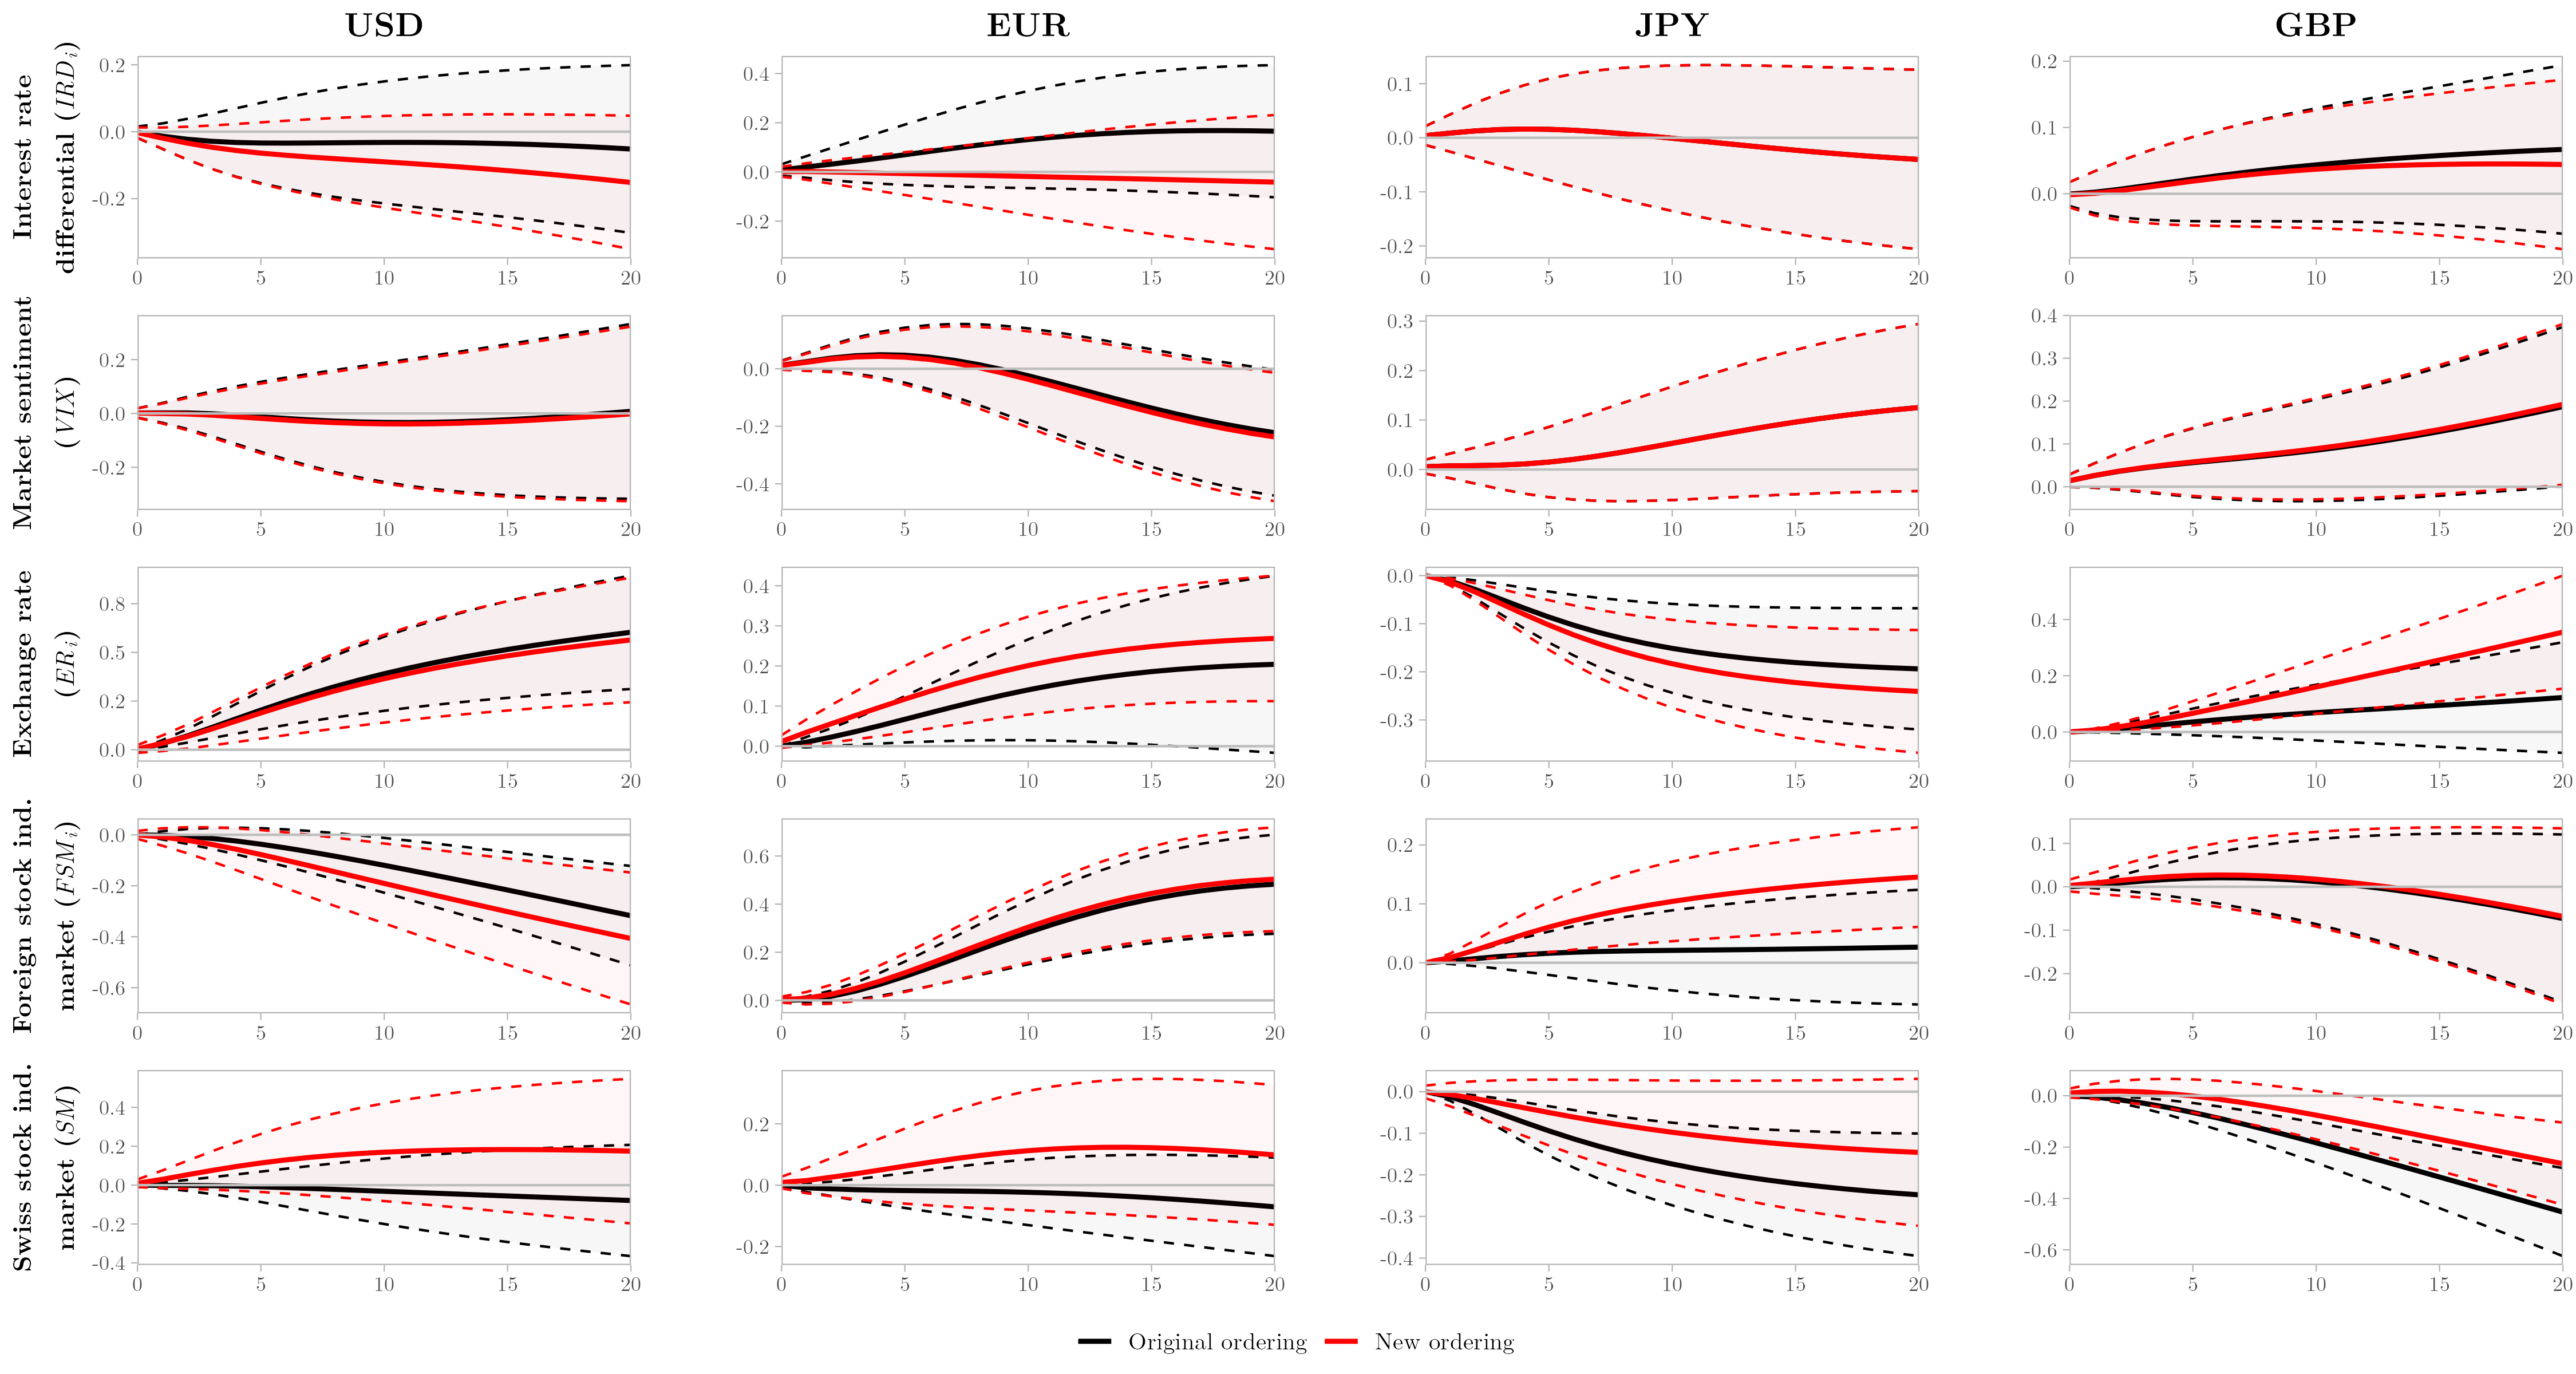
\includegraphics[width=0.99\columnwidth]{figure/gALL_COIRF20_RESP20_NO} 

}

\caption{Responses of Swiss franc carry trade (\textit{CT\textsubscript{i}}) to impulses of financial variables in each target currency model with a new ordering of variables}\label{fig:FigureD1}
\end{figure}

\begin{figure}[!ht]

{\centering 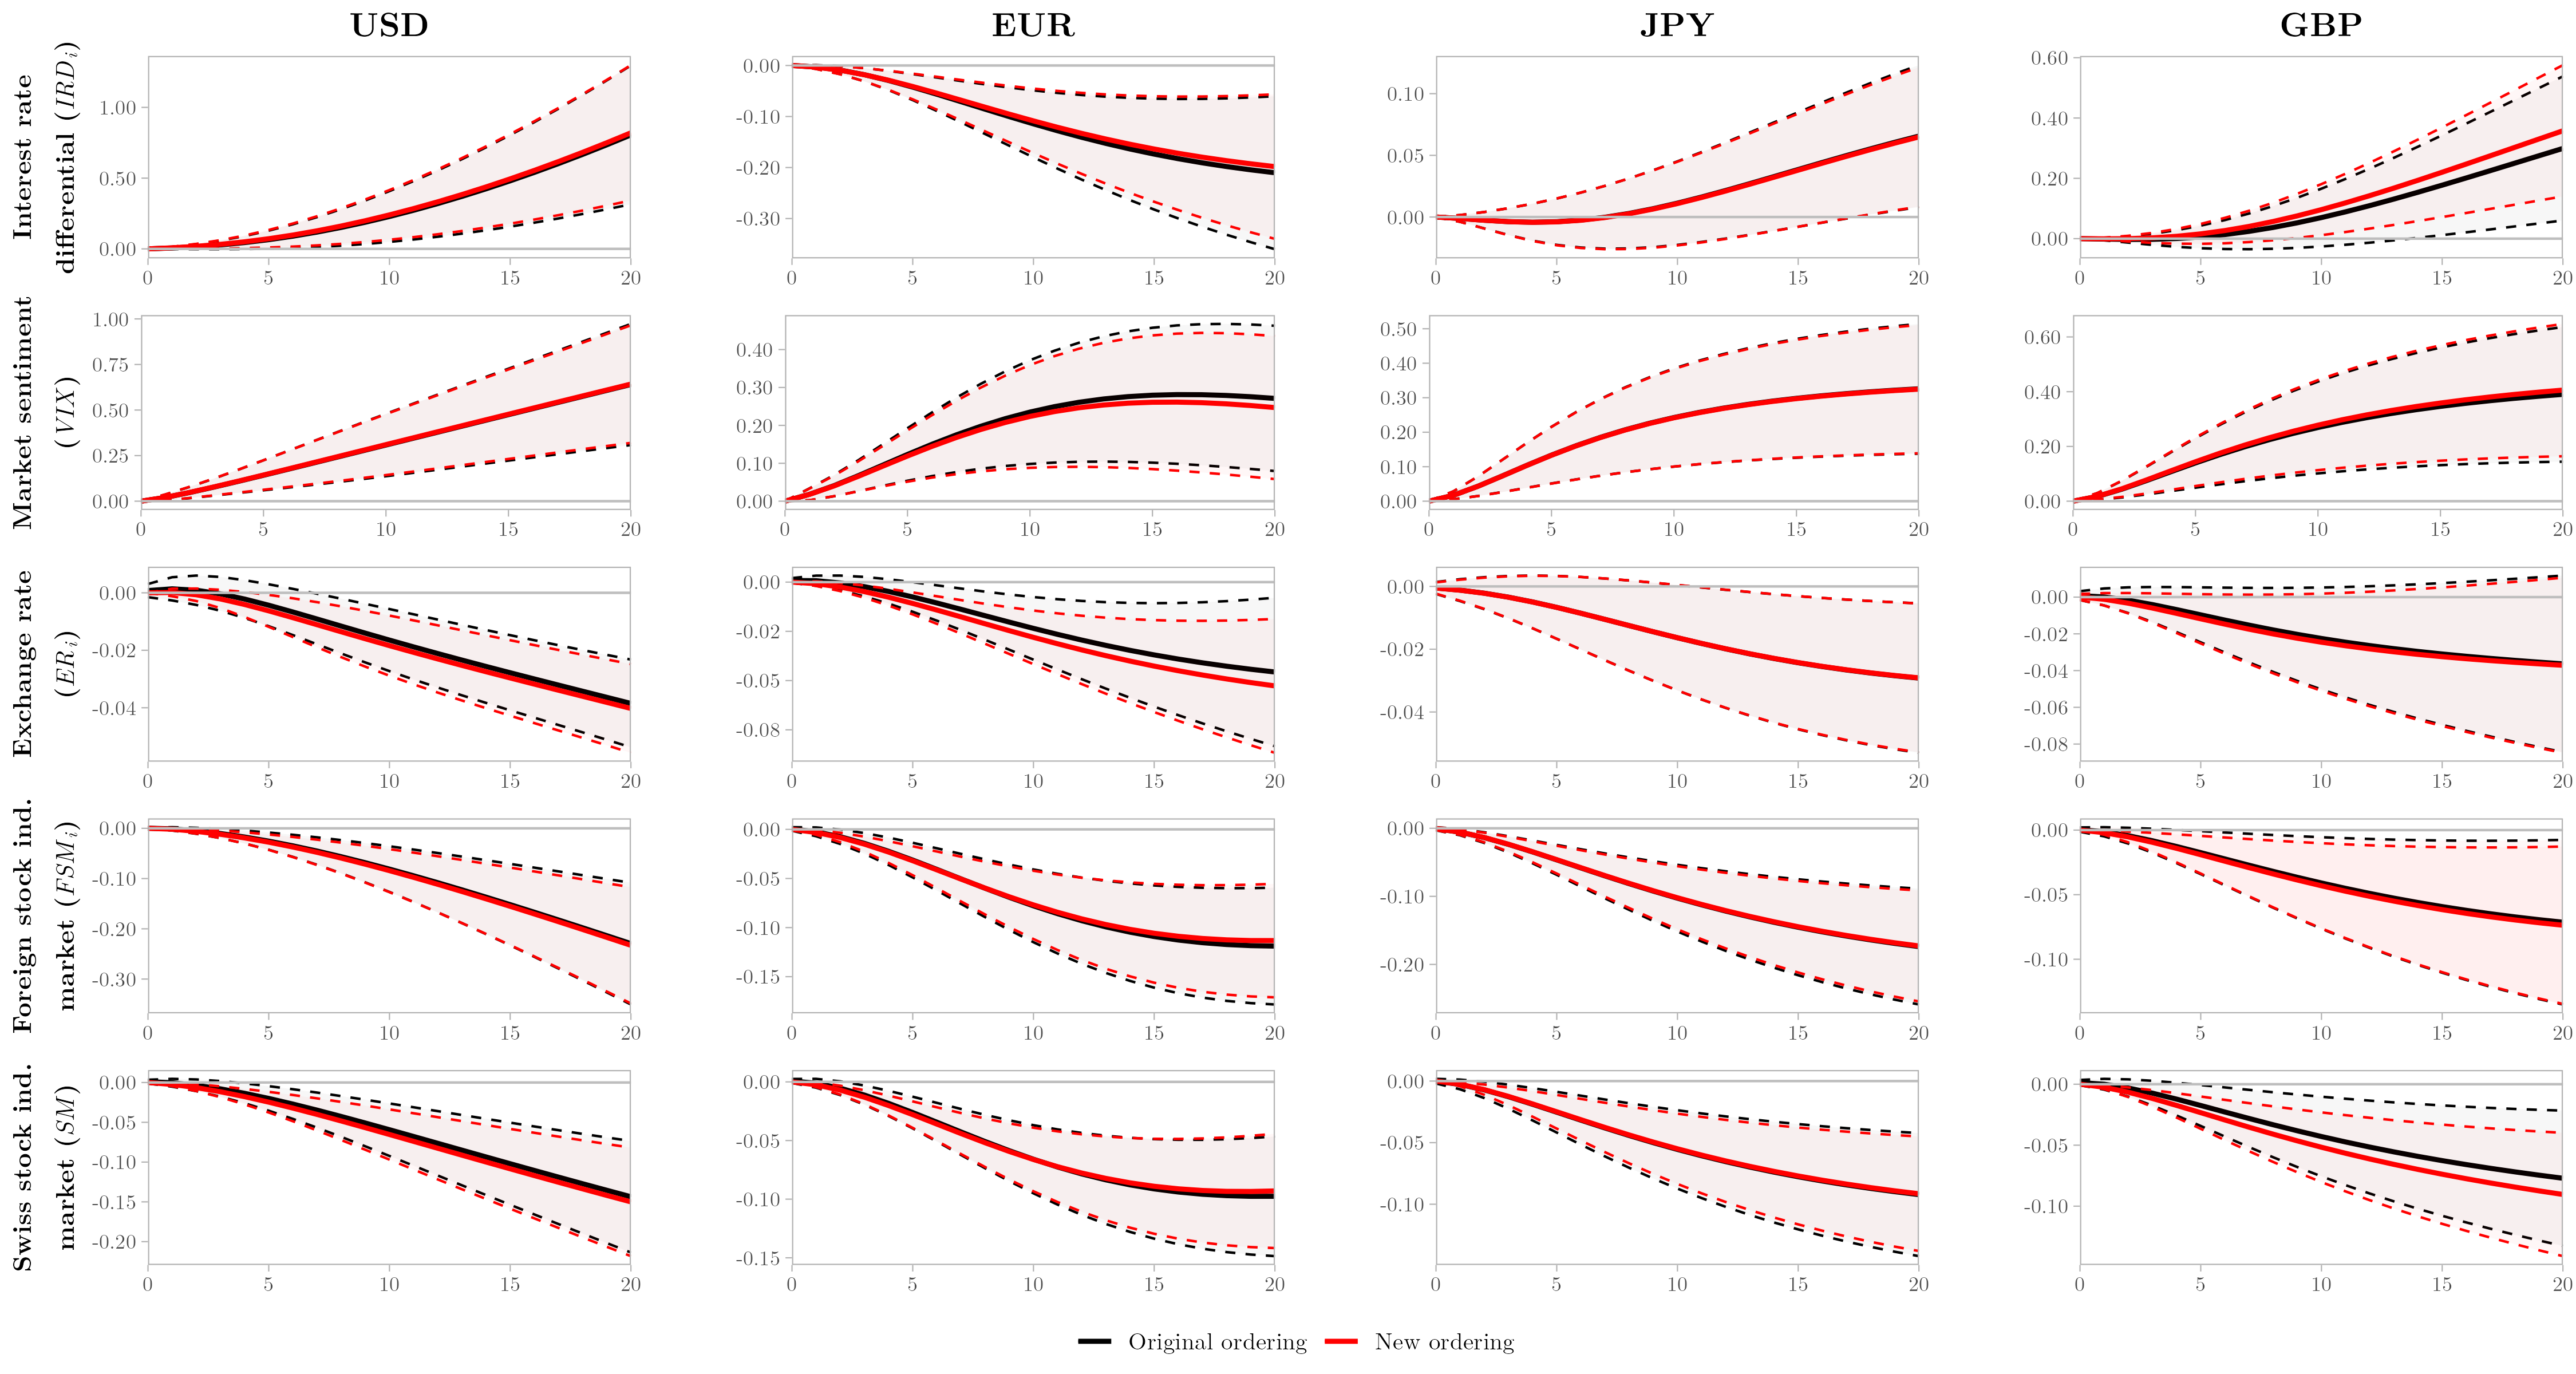
\includegraphics[width=0.99\columnwidth]{figure/gALL_COIRF20_NO} 

}

\caption{Responses of financial variables to impulses of Swiss franc carry trade (\textit{CT\textsubscript{i}}) in each target currency model with a new ordering of variables}\label{fig:FigureD2}
\end{figure}

\clearpage

\begin{figure}[!ht]

{\centering 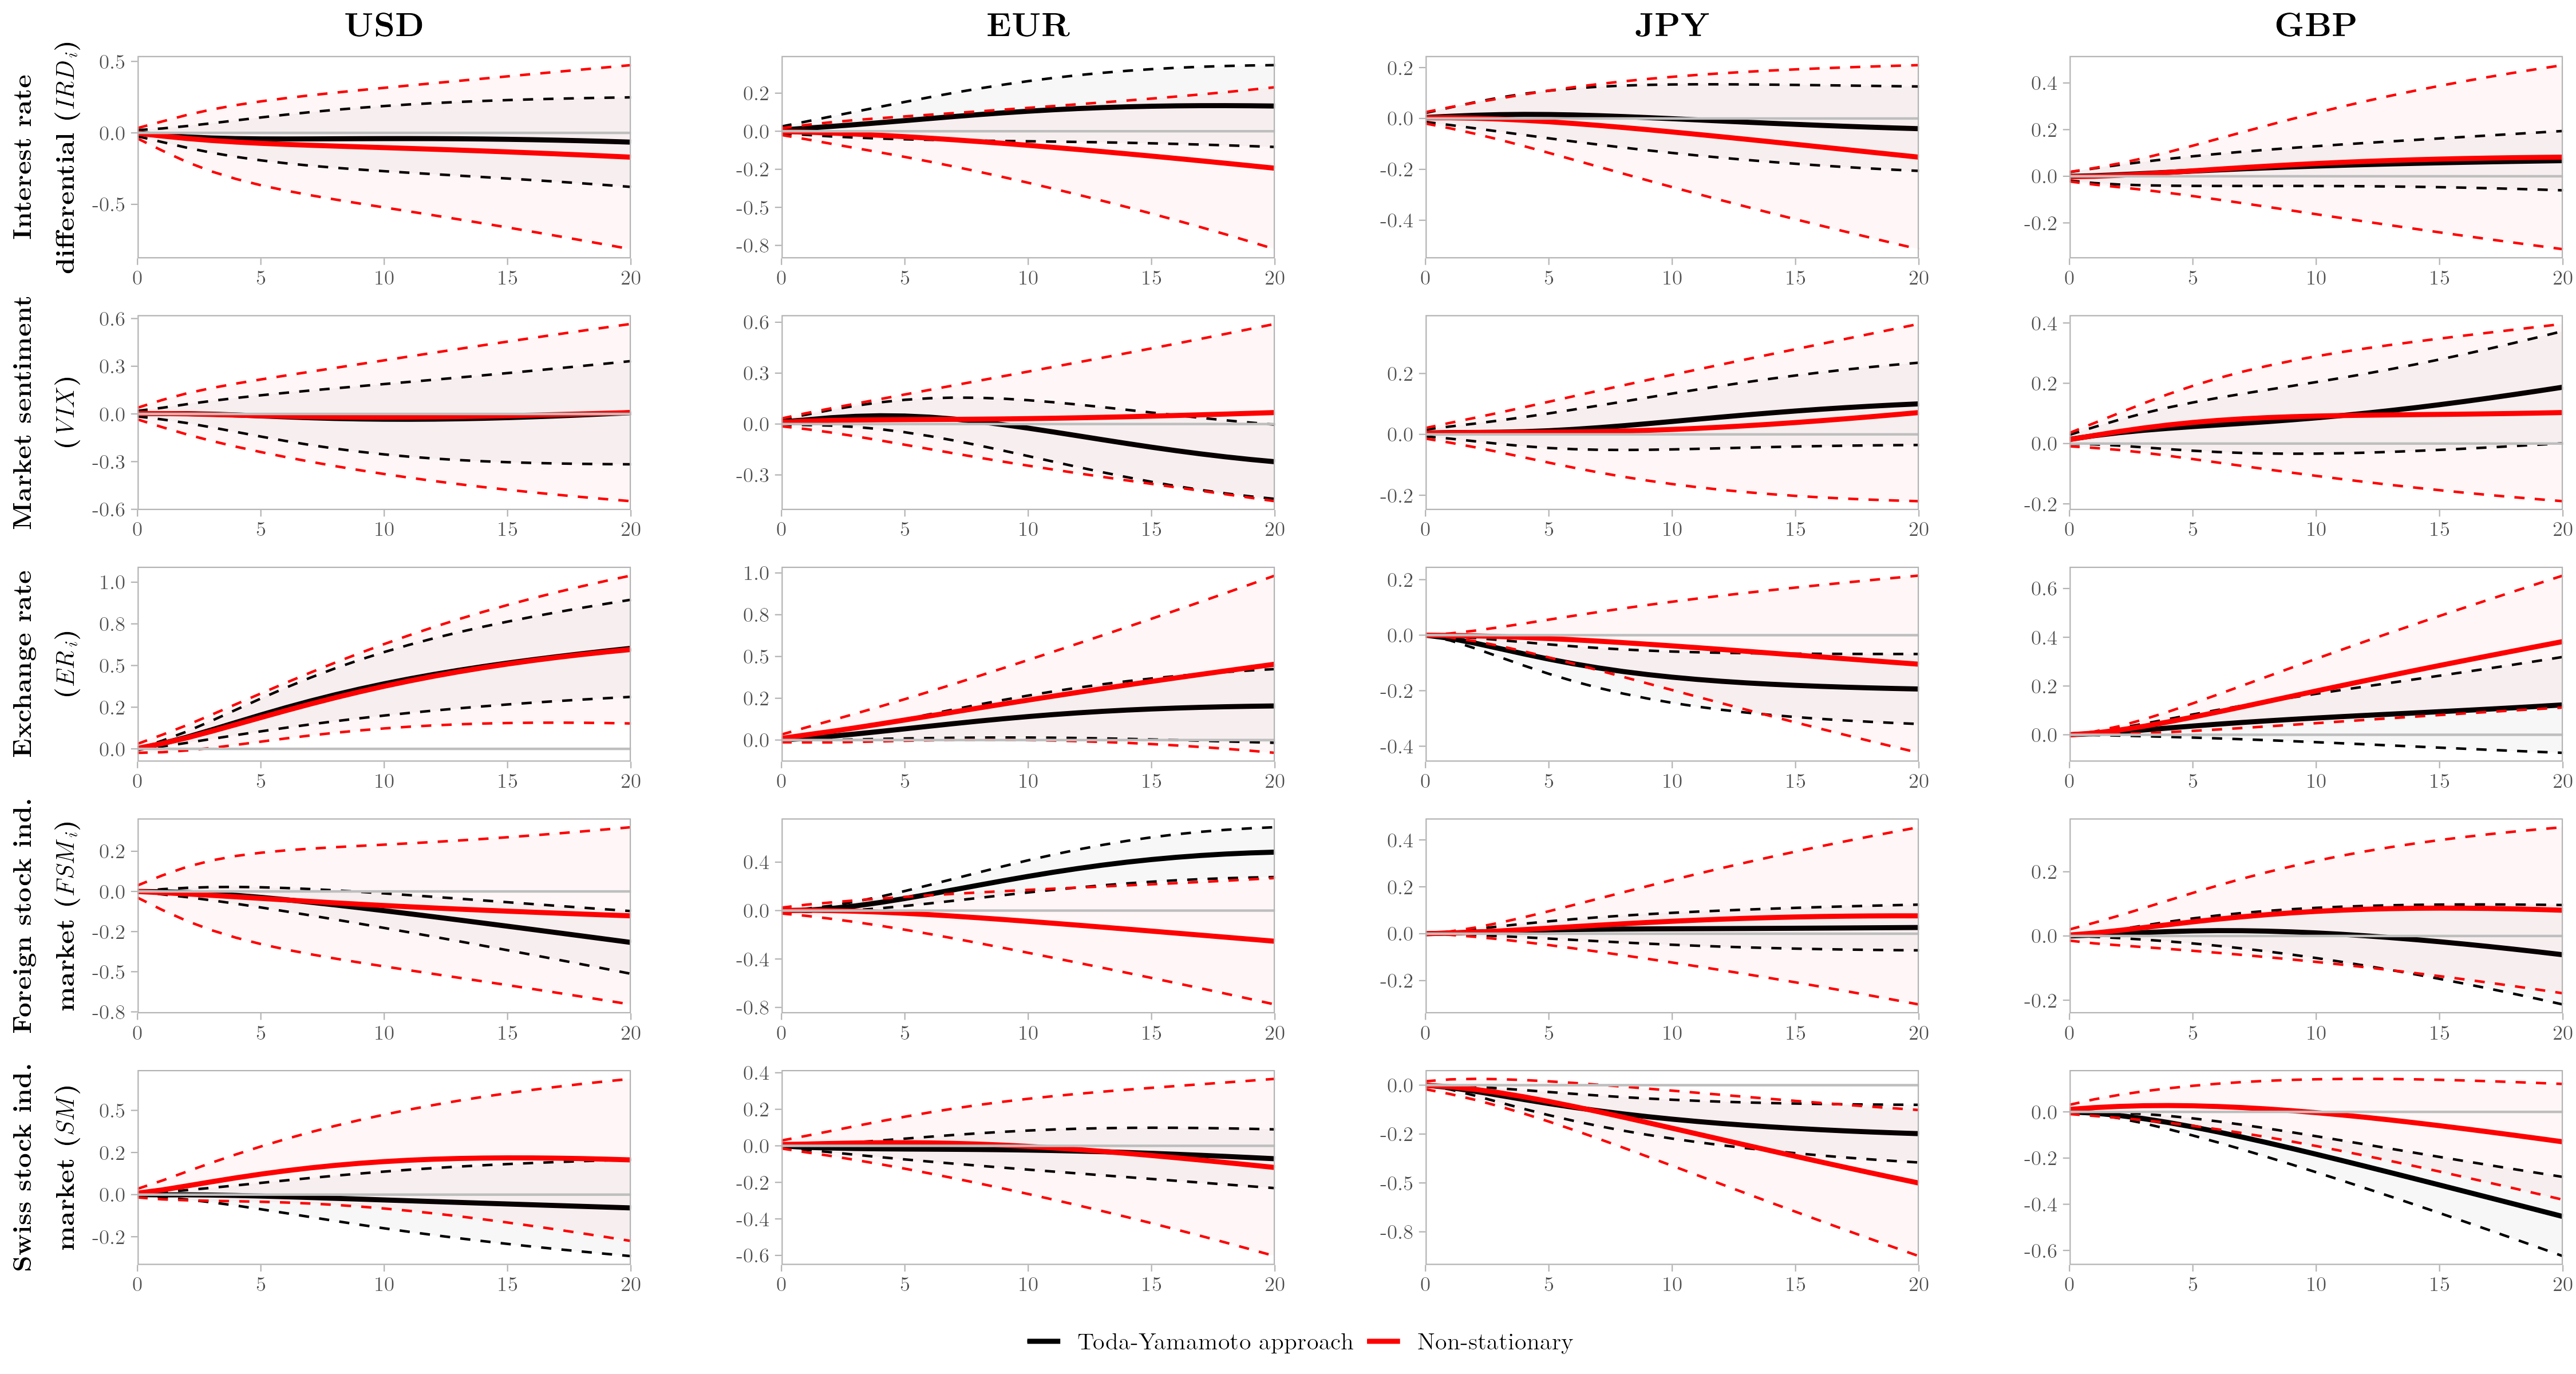
\includegraphics[width=0.99\columnwidth]{figure/gALL_COIRF20_RESP20_NTYA} 

}

\caption{Responses of Swiss franc carry trade (\textit{CT\textsubscript{i}}) to impulses of financial variables in each target currency model with non-stationary variables}\label{fig:FigureD3}
\end{figure}

\begin{figure}[!ht]

{\centering 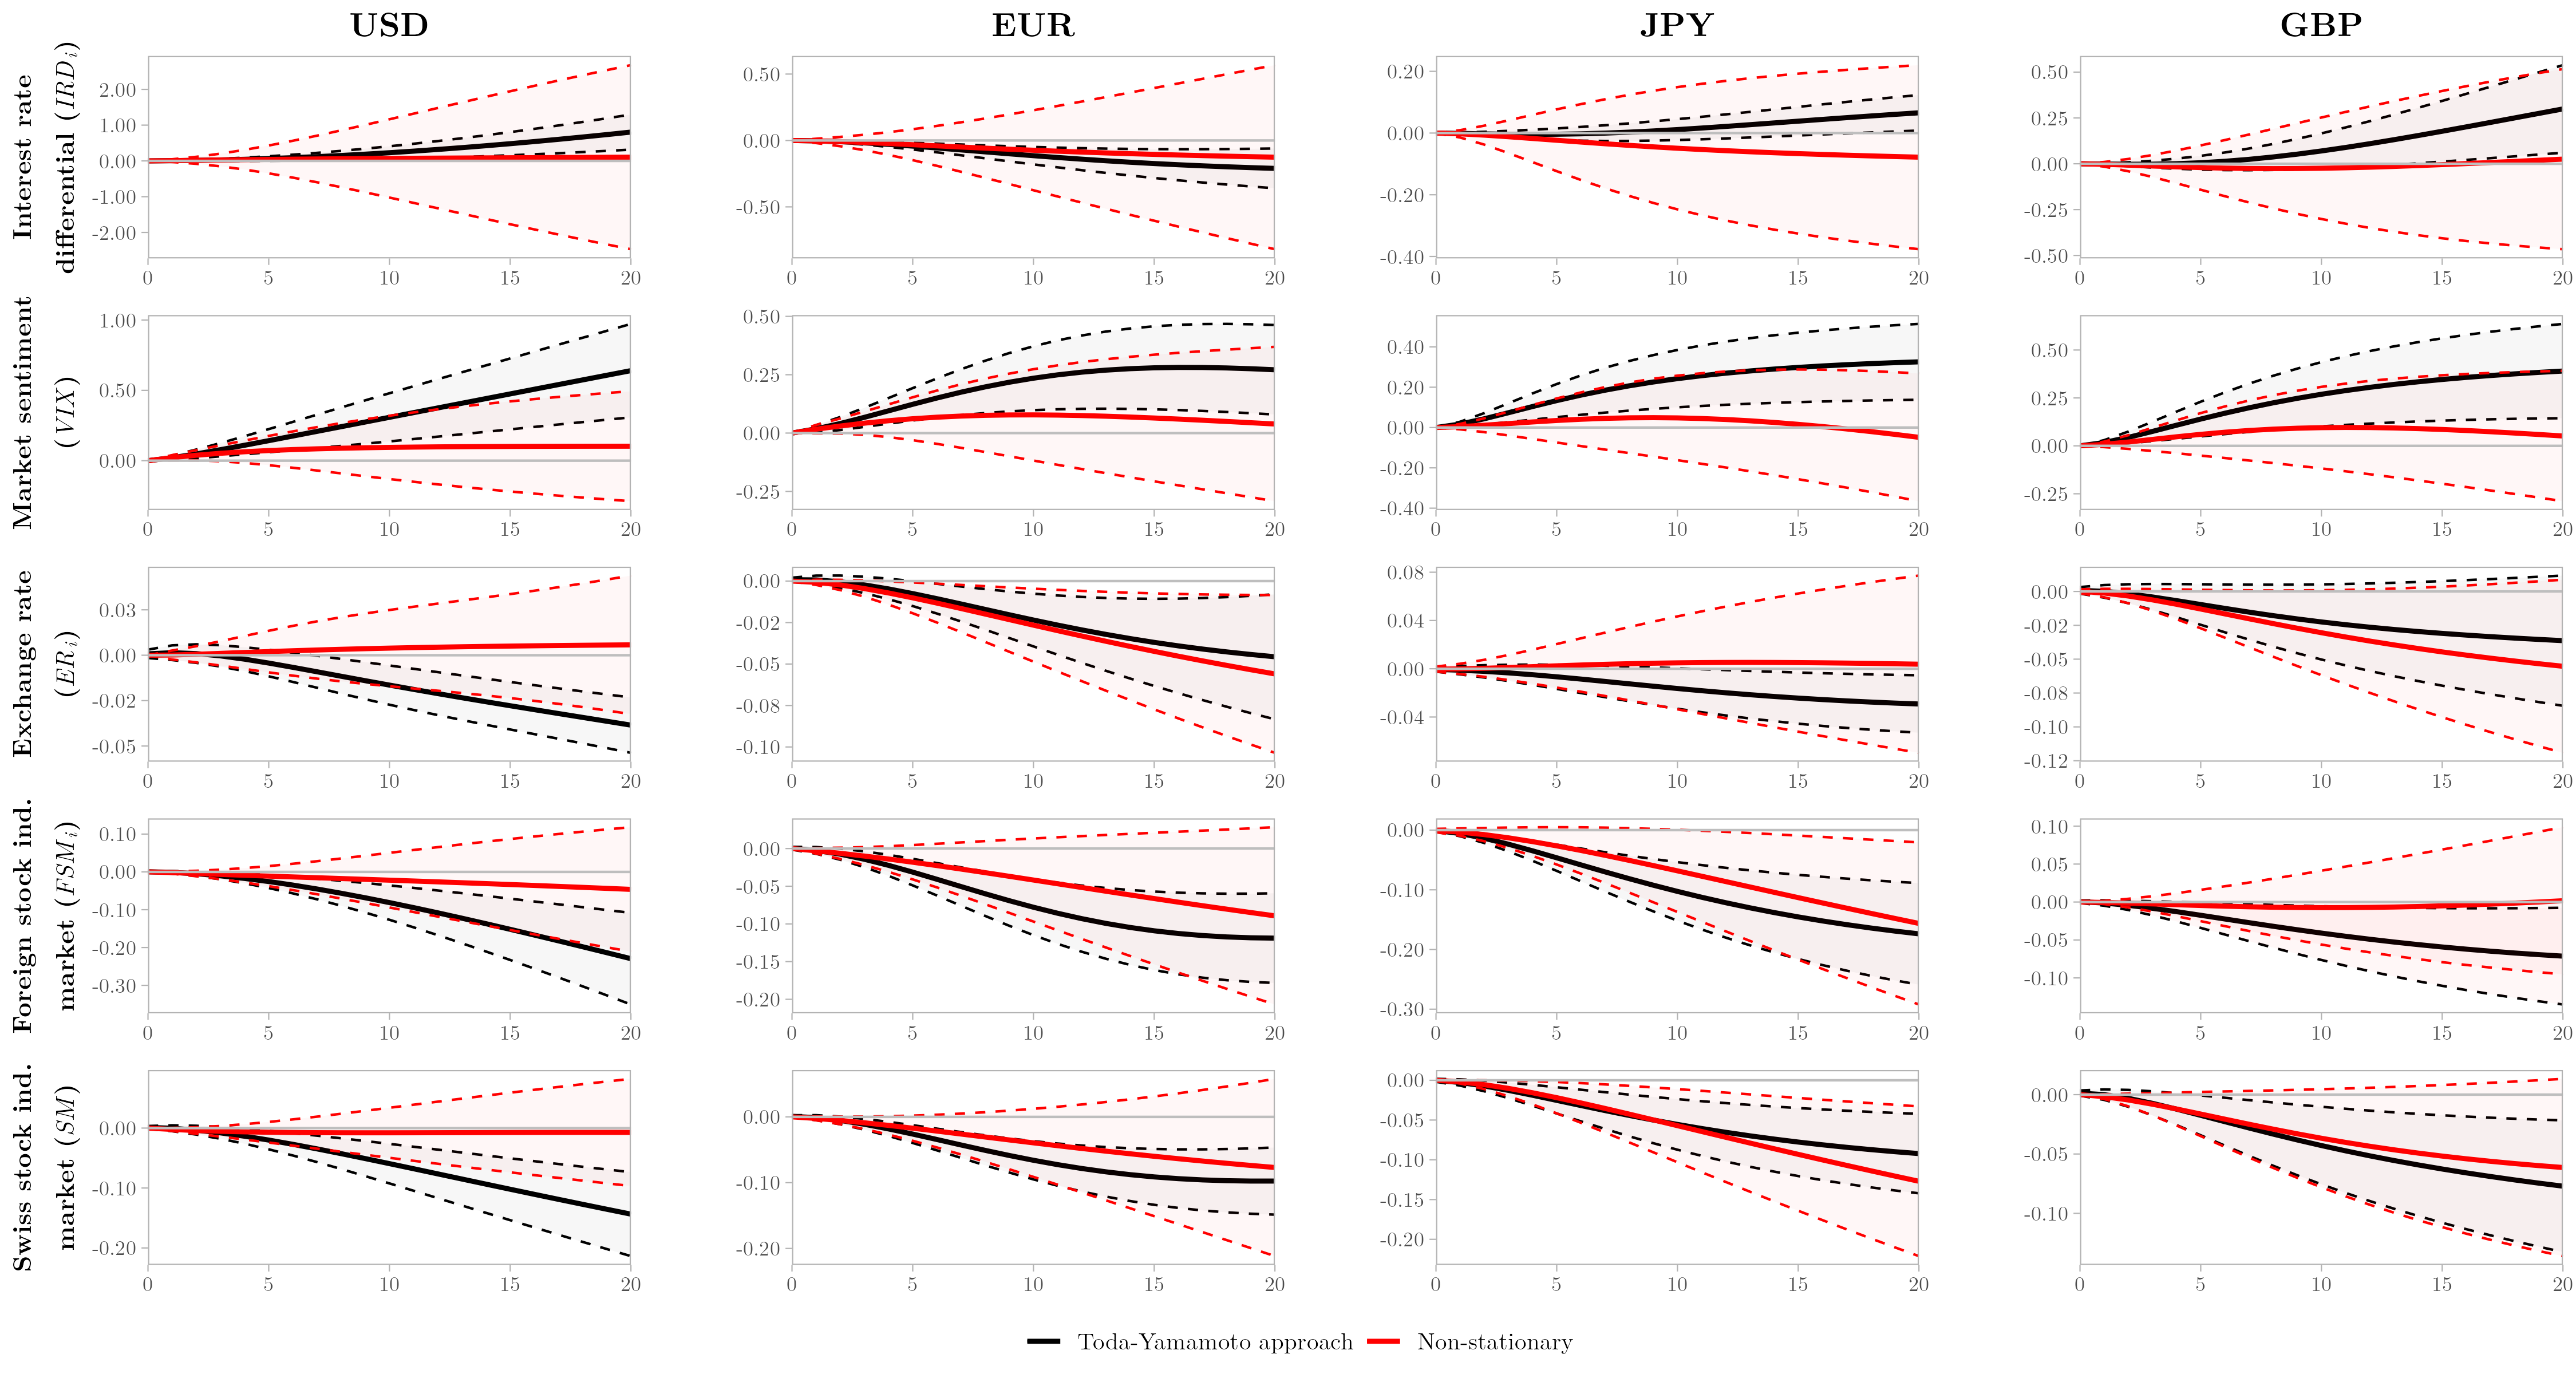
\includegraphics[width=0.99\columnwidth]{figure/gALL_COIRF20_NTYA} 

}

\caption{Responses of financial variables to impulses of Swiss franc carry trade (\textit{CT\textsubscript{i}}) in each target currency model with non-stationary variables}\label{fig:FigureD4}
\end{figure}

\clearpage

\begin{figure}[!ht]

{\centering 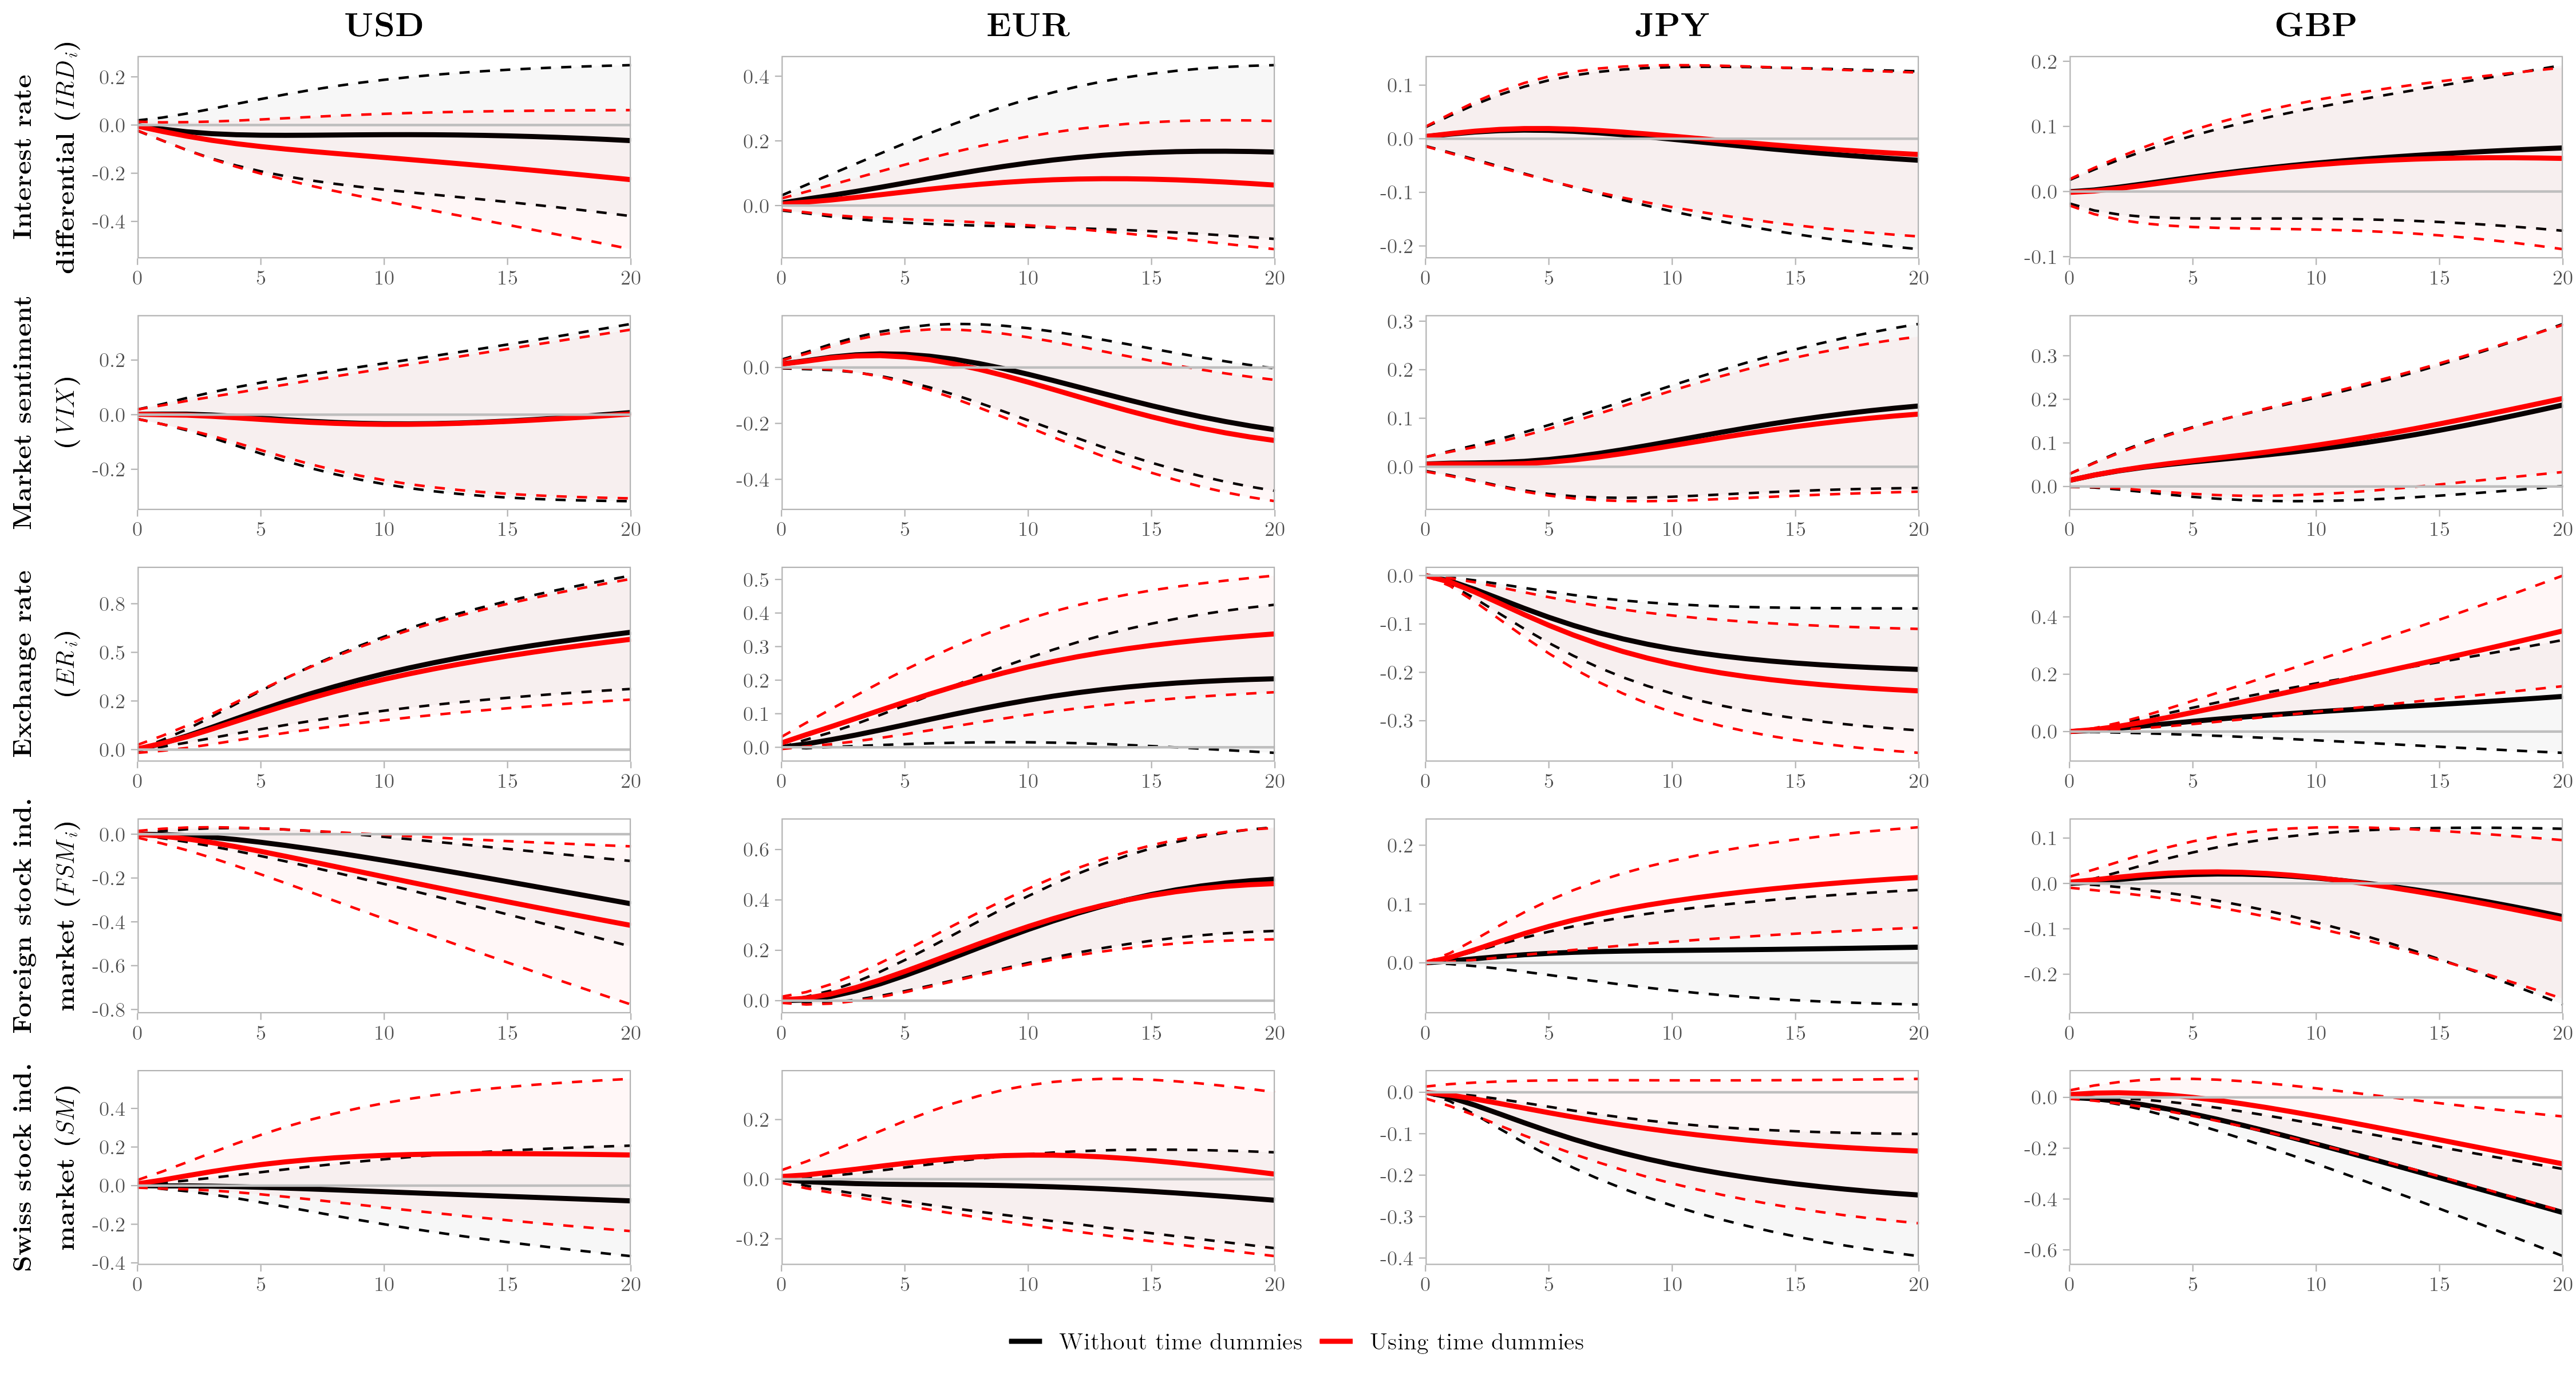
\includegraphics[width=0.99\columnwidth]{figure/gALL_COIRF20_RESP20_DUMMY} 

}

\caption{Responses of Swiss franc carry trade (\textit{CT\textsubscript{i}}) to impulses of financial variables in each target currency model with the inclusion of a time dummy}\label{fig:FigureD5}
\end{figure}

\begin{figure}[!ht]

{\centering 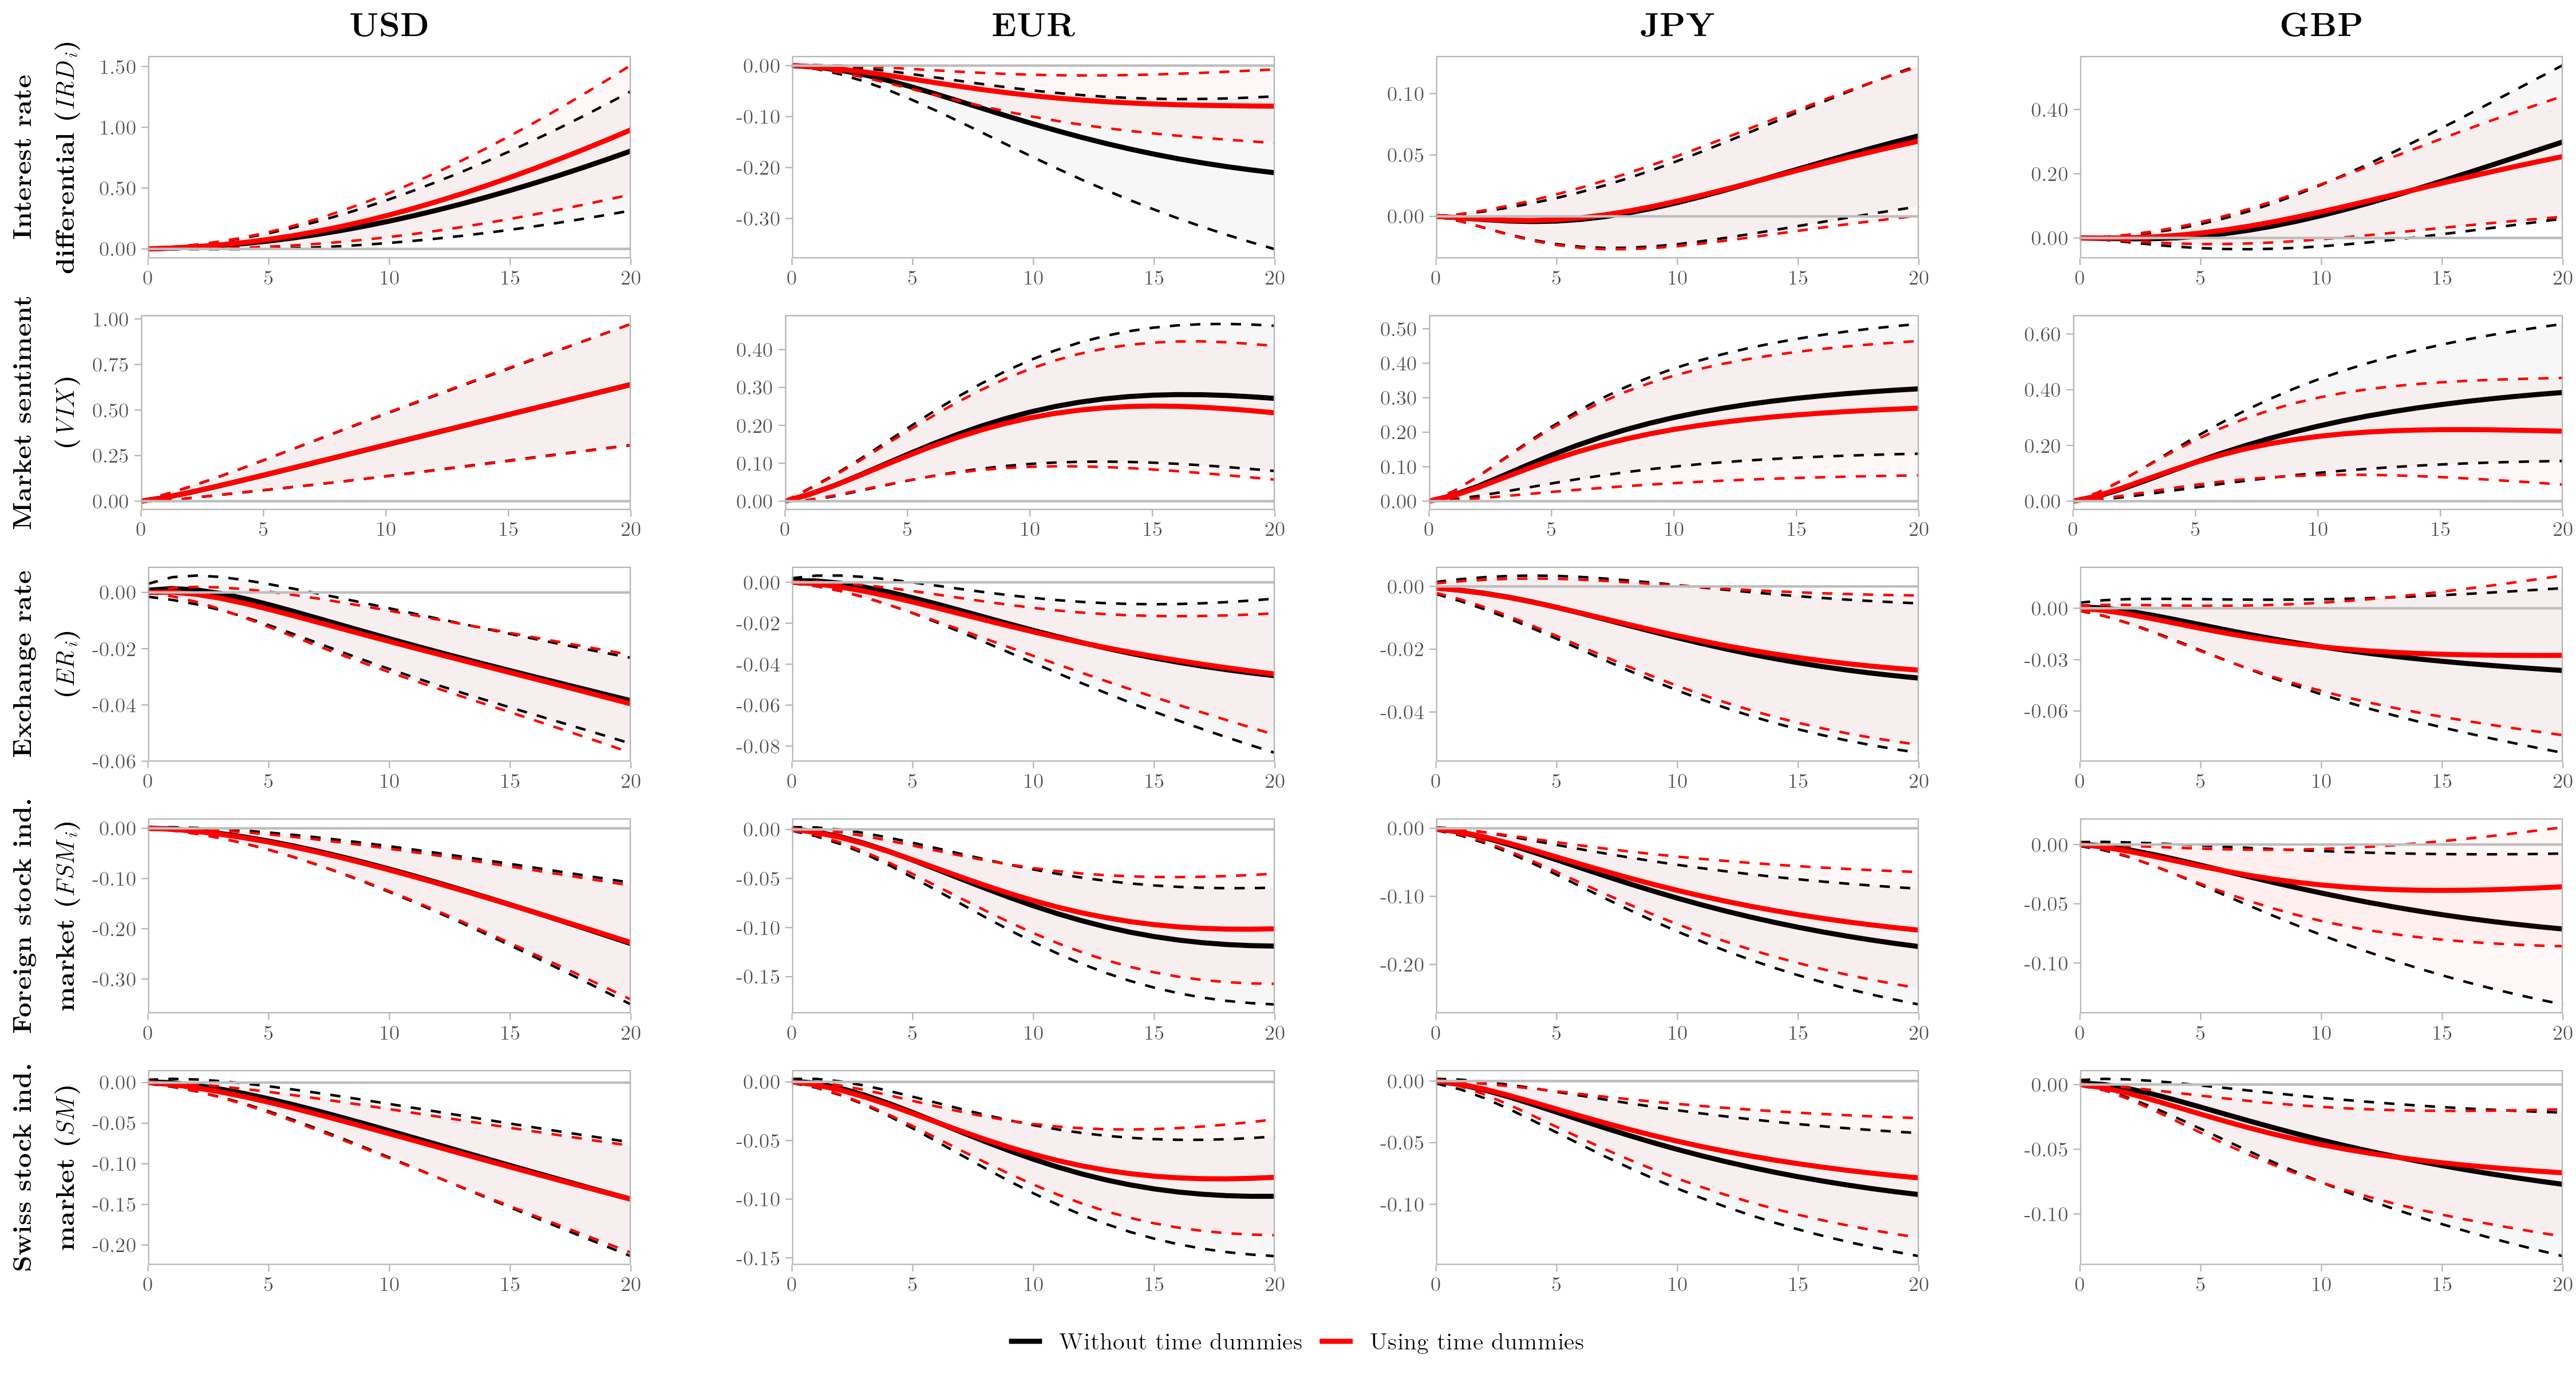
\includegraphics[width=0.99\columnwidth]{figure/gALL_COIRF20_DUMMY} 

}

\caption{Responses of financial variables to impulses of Swiss franc carry trade (\textit{CT\textsubscript{i}}) in each target currency model with the inclusion of a time dummy}\label{fig:FigureD6}
\end{figure}

\clearpage

\begin{figure}[!ht]

{\centering 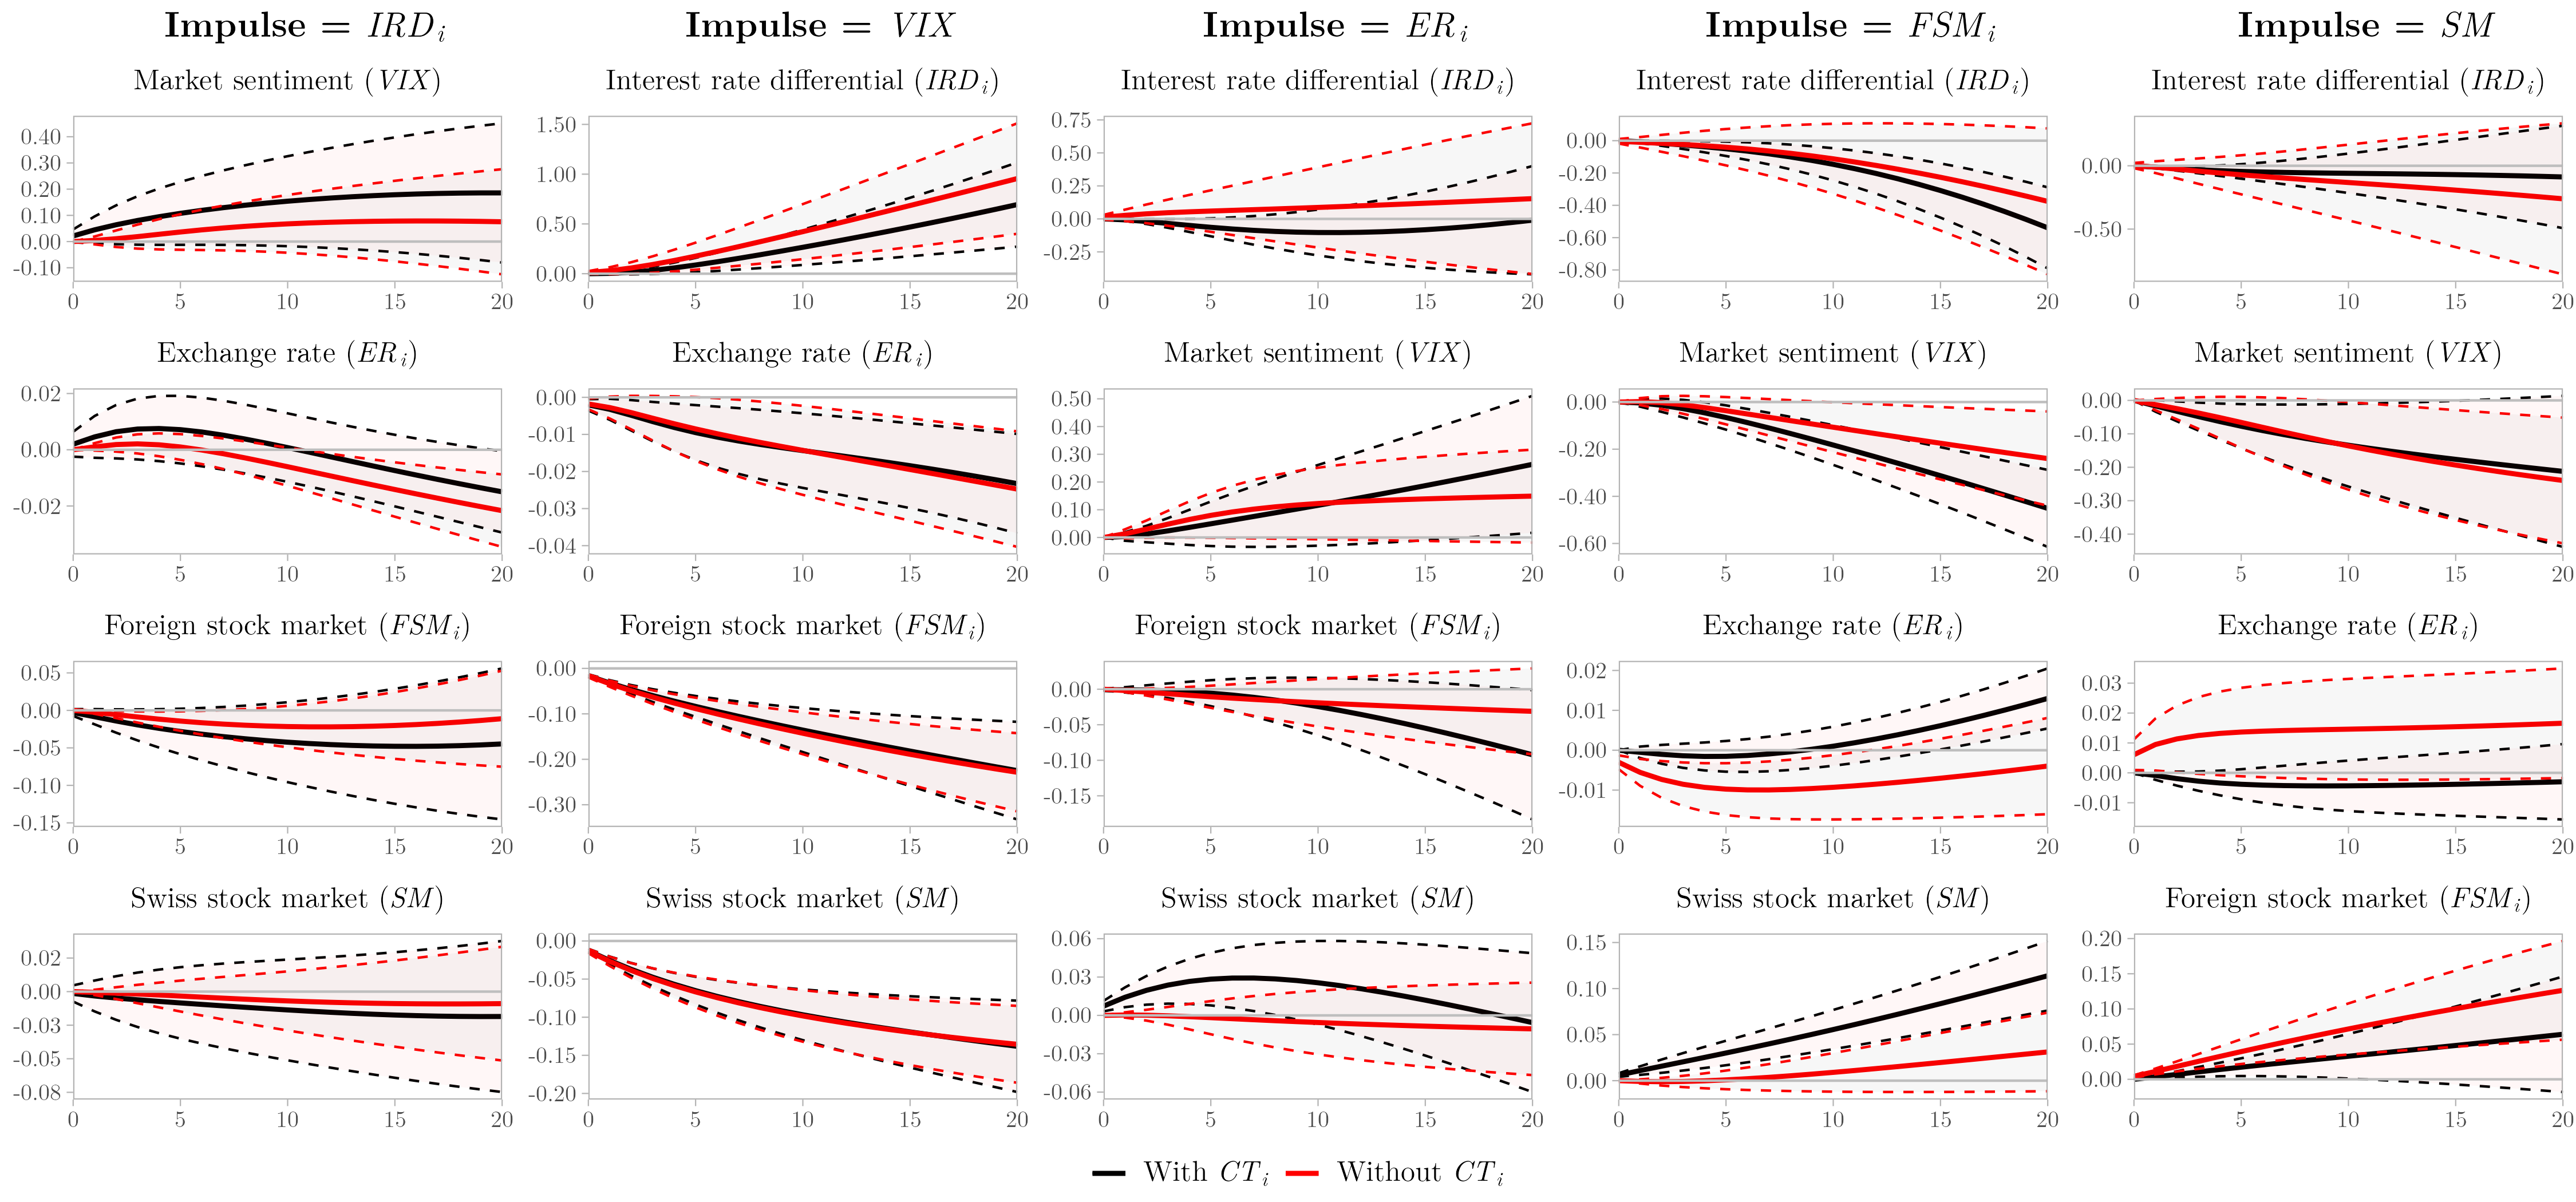
\includegraphics[width=0.99\columnwidth]{figure/gUSD_COIRF_ROB1_ALL_FINAL} 

}

\caption{USD model estimated without Swiss franc carry trade (\textit{CT\textsubscript{i}})}\label{fig:FigureD7}
\end{figure}

\begin{figure}[!ht]

{\centering 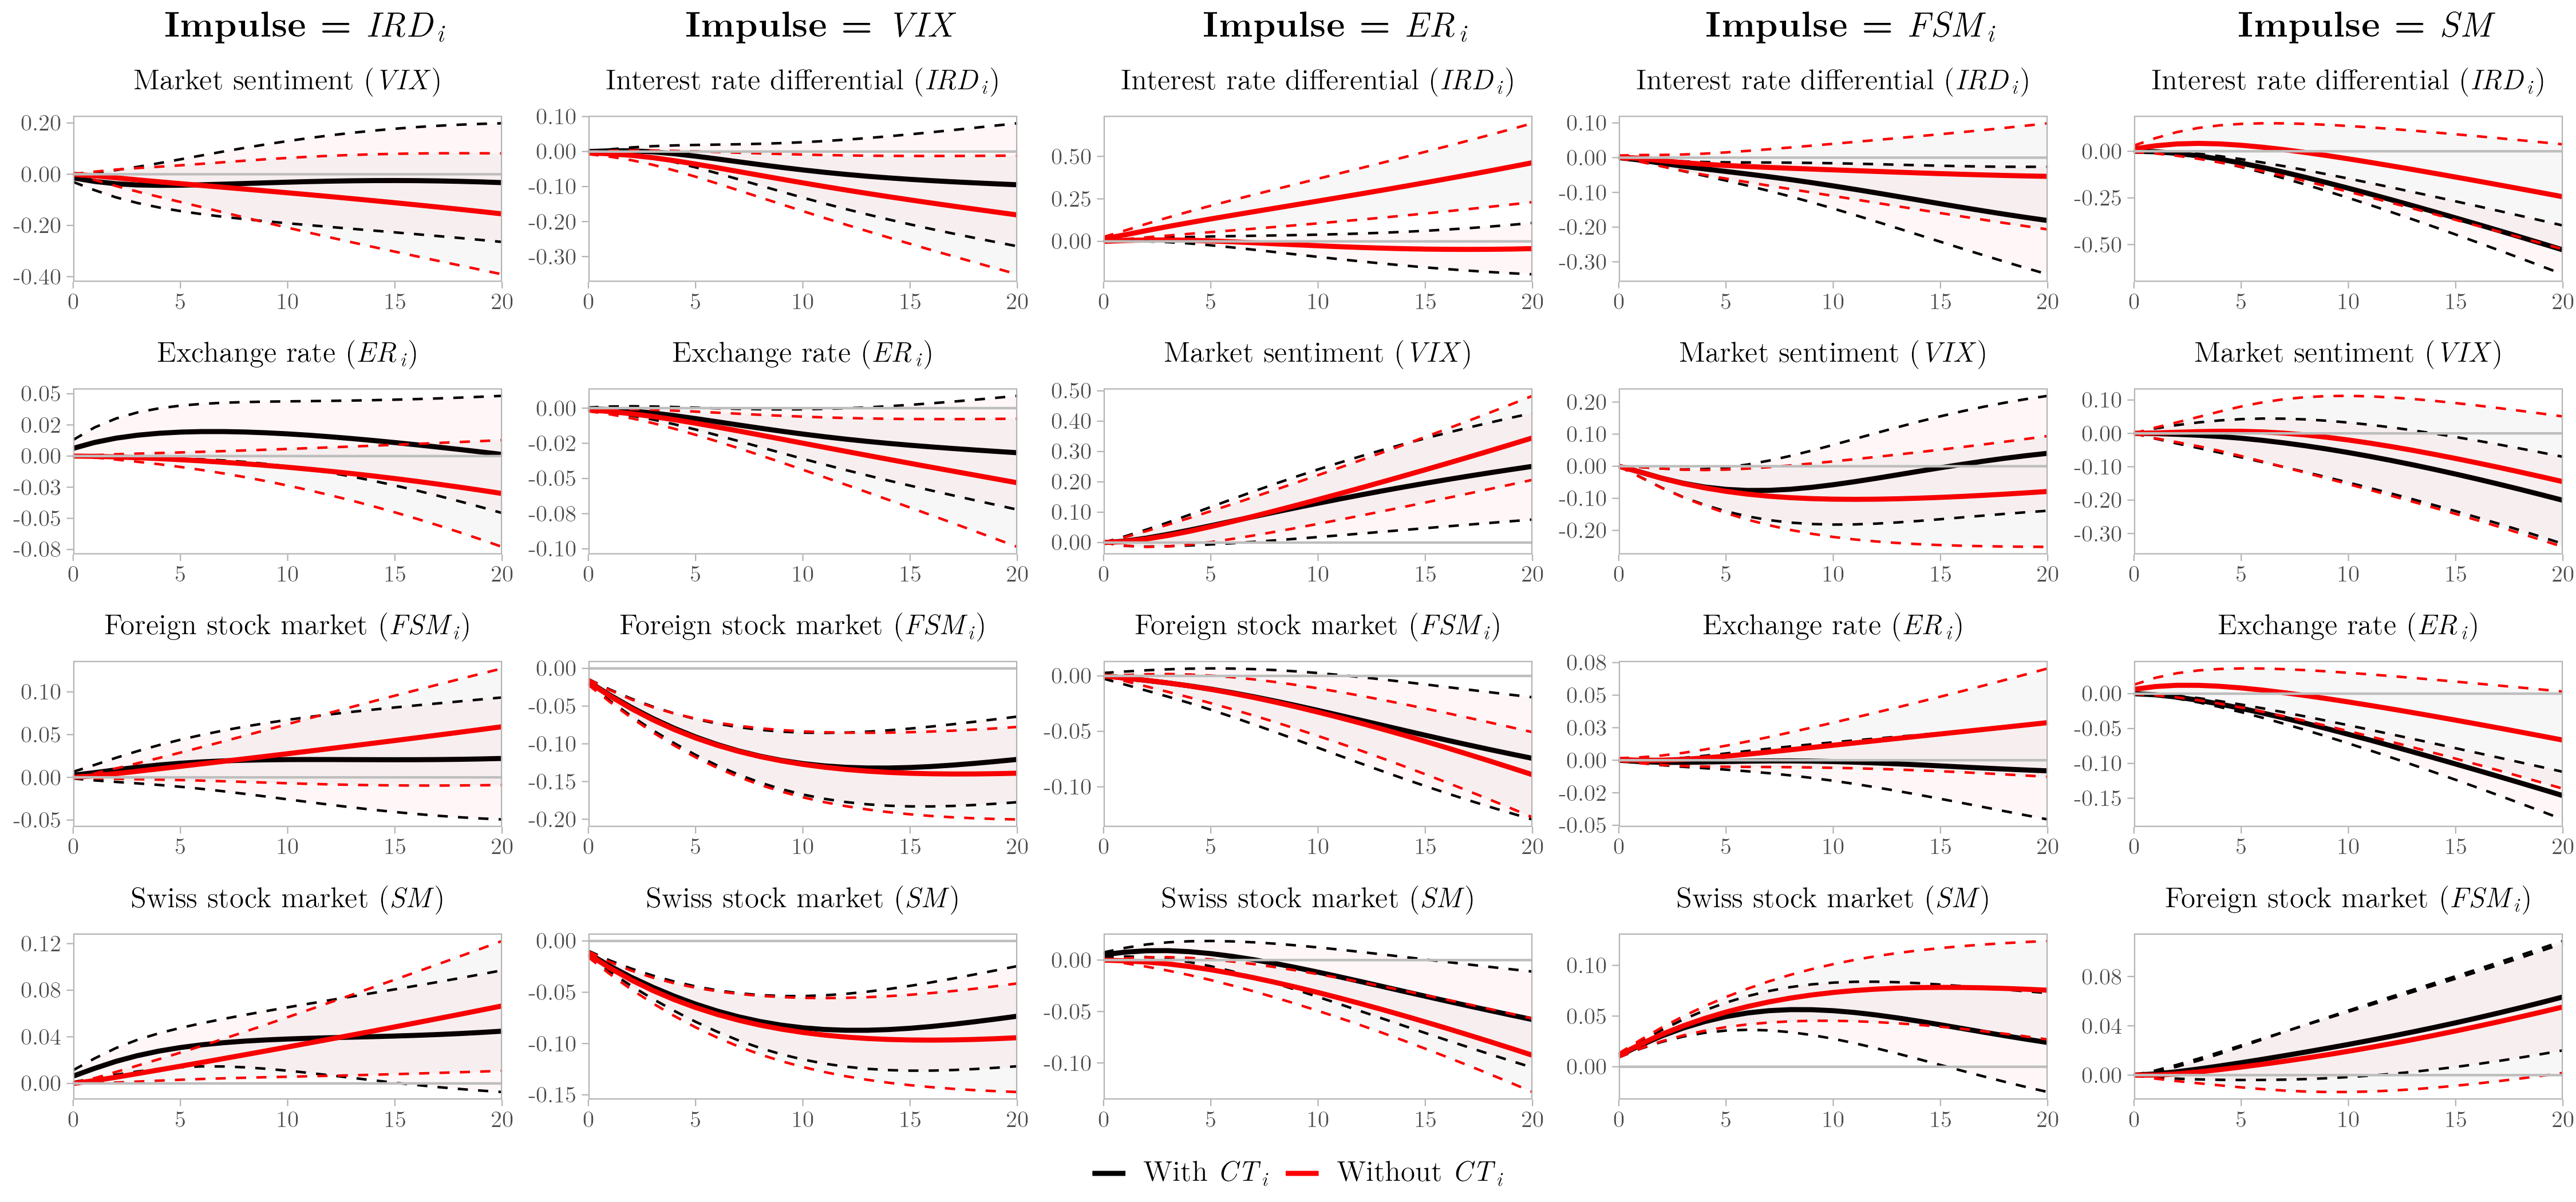
\includegraphics[width=0.99\columnwidth]{figure/gEUR_COIRF_ROB1_ALL_FINAL} 

}

\caption{EUR model estimated without Swiss franc carry trade (\textit{CT\textsubscript{i}})}\label{fig:FigureD8}
\end{figure}

\clearpage

\begin{figure}[!ht]

{\centering \includegraphics[width=0.99\columnwidth]{figure/gJPY_COIRF_ROB1_ALL_FINAL} 

}

\caption{JPY model estimated without Swiss franc carry trade (\textit{CT\textsubscript{i}})}\label{fig:FigureD9}
\end{figure}

\begin{figure}[!ht]

{\centering \includegraphics[width=0.99\columnwidth]{figure/gGBP_COIRF_ROB1_ALL_FINAL} 

}

\caption{GBP model estimated without Swiss franc carry trade (\textit{CT\textsubscript{i}})}\label{fig:FigureD10}
\end{figure}

\hypertarget{appendixd}{%
\chapter{Supplemental Material for Chapter 4}\label{appendixd}}

\hypertarget{appendixd00}{%
\section{Data details}\label{appendixd00}}

Table \ref{tab:TableSD00} presents the full details on the data collection employed in this research. Variables are separated by period levels. The procedure implemented to gather data in different frequency follows the end-period approach. For example, \(NP\) is obtained in weekly levels. In order to use it in the models with quarterly data, the last available observation of the quarter is gathered. Likewise, in an example of the month data, the last input of \(IR\) in each month is considered.



\begin{landscape}\begin{table}[!ht]

\caption{\label{tab:TableSD00}Detailed data description}
\centering
\fontsize{10}{12}\selectfont
\begin{threeparttable}
\begin{tabular}[t]{c>{\raggedright\arraybackslash}p{8cm}>{\centering\arraybackslash}p{5cm}>{\centering\arraybackslash}p{3cm}>{\centering\arraybackslash}p{3cm}}
\toprule
Variable & Definition & Measure & Series code & Source\\
\midrule
\addlinespace[0.3em]
\multicolumn{5}{l}{\textbf{Quarterly levels}}\\
\hspace{1em}$GDP$ & Gross domestic product (expenditure approach)$\textsuperscript{*}$ &  & B1$\_$GE & \\


\hspace{1em}$C$ & Final consumption expenditure$\textsuperscript{*}$ &  & P3 & \\


\hspace{1em}$GFCF$ & Gross fixed capital formation$\textsuperscript{*}$ &  & P51 & \\


\hspace{1em}$X$ & Exports of goods and services$\textsuperscript{*}$ &  & P6 & \\


\hspace{1em}$M$ & Imports of goods and services$\textsuperscript{*}$ & \multirow{-5}{5cm}{\centering\arraybackslash National currency, current prices, s.a. (CQRSA)} & P7 & \multirow{-5}{3cm}{\centering\arraybackslash OECD/QNA}\\


\hspace{1em}\multirow{2}{*}[0pt]{$RES$} & Official reserve assets and other foreign currency assets$\textsuperscript{*}$ & US Dollars, monetary authorities (S1X) & \multirow{2}{*}[0pt]{RAF$\_$USD} & \multirow{2}{*}[0pt]{OECD/MEI$\_$FIN}\\


\addlinespace[0.3em]
\multicolumn{5}{l}{\textbf{Monthly levels}}\\
\hspace{1em}\multirow{2}{*}[0pt]{$EQ$} & Leading indicators OECD, component series, share prices, original series$\textsuperscript{*}$ & \multirow{2}{*}[0pt]{Index 2015 = 100, s.a.} & \multirow{2}{*}[0pt]{SP} & \multirow{2}{*}[0pt]{IMF/IRFCL}\\


\hspace{1em}$X$ & Exports of goods and services$\textsuperscript{*}$ &  & XTEXVA01 & \\


\hspace{1em}$M$ & Imports of goods and services$\textsuperscript{*}$ & \multirow{-2}{5cm}{\centering\arraybackslash US Dollars, s.a. (CXMLSA)} & XTIMVA01 & \multirow{-2}{3cm}{\centering\arraybackslash OECD/MEI}\\


\hspace{1em}\multirow{2}{*}[0pt]{$IP$} & \multirow{2}{*}[0pt]{Production, total industry excluding construction} & Index 2015 = 100, s.a. (IXOBSA) & \multirow{2}{*}[0pt]{PRINTO01} & \multirow{2}{*}[0pt]{OECD/MEI}\\


\hspace{1em}\multirow{2}{*}[0pt]{$GCF$} & Global common factor estimated from world-wide cross section of risky asset prices & \multirow{2}{*}[0pt]{Standardized unit} & Global factor, new datalist & \textcite{miranda-agrippino2021a}\\


\addlinespace[0.3em]
\multicolumn{5}{l}{\textbf{Weekly levels}}\\
\hspace{1em}\multirow{2}{*}[0pt]{$NP$} & Net (long minus short) positions as a share of open interest contracts (carry trade proxy) & Number of contracts of futures and options, leveraged funds & CFTC code for each currency$\textsuperscript{$\dagger$}$ & \multirow{2}{*}[0pt]{CFTC/COT-TFF}\\


\addlinespace[0.3em]
\multicolumn{5}{l}{\textbf{Daily levels}}\\
\hspace{1em}$IR$ & Central bank policy rates & Percent ($\%$) & CBPOL$\textsuperscript{$\dagger$}$ & \\


\hspace{1em}$ER$ & Nominal exchange rates$\textsuperscript{*}$ & US dollar exchange rates & XRUSD$\textsuperscript{$\dagger$}$ & \multirow{-2}{3cm}{\centering\arraybackslash BIS}\\


\hspace{1em}$EQ$ & Share prices$\textsuperscript{*}$ & Index 2015 = 100 & SP & OECD/MEI$\_$FIN\\


$VIX$ & CBOE Volatility Index - VIX (VIXCLS)$\textsuperscript{*}$ & Index & VIXCLS & FRED\\
\bottomrule
\end{tabular}
\begin{tablenotes}[para]
\item \footnotesize{$Abbreviations$: Seasonally adjusted (s.a.); Quarterly National Accounts (QNA);  International Reserves and Foreign Currency Liquidity (IRFCL); Monetary and Financial Statistics (MEI\_FIN); Main Economic Indicators (MEI); Commitments of Traders (COT), Traders in Financial Futures (TFF) report.} $\newline$ \footnotesize{$*$ Variables in logarithmic transform.} $\newline$ \footnotesize{$\dagger$ See Table \ref{tab:TableSD001} for the list of codes.}
\end{tablenotes}
\end{threeparttable}
\end{table}
\end{landscape}

\begin{table}[!ht]

\caption{\label{tab:TableSD001}Specific codes for $IR$, $ER$ and $NP$}
\centering
\resizebox{\linewidth}{!}{
\begin{tabular}[t]{llll}
\toprule
Country & $IR$ & $ER$ & $NP$\\
\midrule
Australia & D:AU & D:AU:AUD:A & Australian dollar (232741)\\
Brazil & D:BR & D:BR:BRL:A & Brazilian real (102741)\\
Canada & D:CA & D:CA:CAD:A & Canadian dollar (090741)\\
China & D:CN & D:CN:CNY:A & \\
Czech Republic & D:CZ & D:CZ:CZK:A & \\
Denmark & D:DK & D:DK:DKK:A & \\
Euro area & D:XM & D:XM:EUR:A & Euro (099741)\\
Hungary & D:HU & D:HU:HUF:A & \\
India & D:IN & D:IN:INR:A & \\
Japan & D:JP & D:JP:JPY:A & Japanese yen (097741)\\
Korea & D:KR & D:KR:KRW:A & \\
Mexico & D:MX & D:MX:MXN:A & Mexican peso (095741)\\
New Zealand & D:NZ & D:NZ:NZD:A & New Zealand dollar (112741)\\
Norway & D:NO & D:NO:NOK:A & \\
Poland & D:PL & D:PL:PLN:A & \\
Russia & D:RU & D:RU:RUB:A & Russian ruble (089741)\\
South Africa & D:ZA & D:ZA:ZAR:A & \\
Sweden & D:SE & D:SE:SEK:A & \\
Switzerland & D:CH & D:CH:CHF:A & Swiss franc (092741)\\
Turkey & D:TR & D:TR:TRY:A & \\
United Kingdom & D:GB & D:GB:GBP:A & British pound sterling (096742)\\
United States & D:US &  & U.S. dollar index, ICE Futures U.S. (098662)\\
\bottomrule
\end{tabular}}
\end{table}

\clearpage

\hypertarget{appendixd0}{%
\section{Trade weight matrix}\label{appendixd0}}

\begin{table}[!ht]

\caption{\label{tab:TableSD0}Trade weight matrix for Switzerland, Models 1 and 3}
\centering
\resizebox{\linewidth}{!}{
\fontsize{7}{9}\selectfont
\begin{tabular}[t]{lcccccccccccccccccccccc}
\toprule
  & AU & BR & CA & CH & CN & CZ & DK & GB & HU & IN & JP & KR & MX & NO & NZ & PL & RU & SE & TR & U2 & US & ZA\\
\midrule
AU & 0.000 & 0.005 & 0.010 & 0.010 & 0.349 & 0.002 & 0.004 & 0.038 & 0.001 & 0.041 & 0.166 & 0.076 & 0.007 & 0.001 & 0.042 & 0.002 & 0.003 & 0.007 & 0.004 & 0.117 & 0.106 & 0.007\\
BR & 0.007 & 0.000 & 0.020 & 0.016 & 0.269 & 0.002 & 0.004 & 0.024 & 0.002 & 0.029 & 0.044 & 0.039 & 0.032 & 0.006 & 0.001 & 0.004 & 0.022 & 0.008 & 0.008 & 0.252 & 0.206 & 0.008\\
CA & 0.004 & 0.007 & 0.000 & 0.006 & 0.084 & 0.001 & 0.002 & 0.028 & 0.001 & 0.007 & 0.029 & 0.013 & 0.037 & 0.006 & 0.001 & 0.002 & 0.003 & 0.003 & 0.003 & 0.070 & 0.691 & 0.002\\
CH & 0.008 & 0.008 & 0.011 & 0.000 & 0.062 & 0.009 & 0.005 & 0.085 & 0.005 & 0.036 & 0.026 & 0.008 & 0.006 & 0.003 & 0.001 & 0.009 & 0.010 & 0.008 & 0.013 & 0.564 & 0.116 & 0.006\\
CN & 0.054 & 0.037 & 0.023 & 0.013 & 0.000 & 0.005 & 0.005 & 0.032 & 0.004 & 0.033 & 0.141 & 0.117 & 0.019 & 0.003 & 0.005 & 0.008 & 0.037 & 0.006 & 0.009 & 0.201 & 0.229 & 0.018\\
CZ & 0.002 & 0.002 & 0.002 & 0.013 & 0.044 & 0.000 & 0.009 & 0.040 & 0.030 & 0.004 & 0.009 & 0.008 & 0.003 & 0.003 & 0.000 & 0.077 & 0.032 & 0.014 & 0.009 & 0.680 & 0.020 & 0.002\\
DK & 0.006 & 0.006 & 0.007 & 0.009 & 0.055 & 0.013 & 0.000 & 0.069 & 0.008 & 0.007 & 0.014 & 0.009 & 0.003 & 0.067 & 0.001 & 0.034 & 0.015 & 0.138 & 0.010 & 0.469 & 0.058 & 0.003\\
GB & 0.013 & 0.007 & 0.022 & 0.039 & 0.081 & 0.010 & 0.012 & 0.000 & 0.006 & 0.016 & 0.021 & 0.011 & 0.004 & 0.034 & 0.002 & 0.018 & 0.017 & 0.020 & 0.017 & 0.513 & 0.123 & 0.013\\
HU & 0.002 & 0.002 & 0.002 & 0.009 & 0.050 & 0.047 & 0.008 & 0.034 & 0.000 & 0.004 & 0.012 & 0.013 & 0.005 & 0.001 & 0.000 & 0.052 & 0.048 & 0.012 & 0.014 & 0.659 & 0.024 & 0.002\\
IN & 0.041 & 0.023 & 0.015 & 0.062 & 0.205 & 0.003 & 0.004 & 0.042 & 0.002 & 0.000 & 0.045 & 0.050 & 0.015 & 0.004 & 0.003 & 0.005 & 0.020 & 0.007 & 0.016 & 0.219 & 0.187 & 0.032\\
JP & 0.063 & 0.014 & 0.022 & 0.013 & 0.320 & 0.003 & 0.003 & 0.022 & 0.003 & 0.016 & 0.000 & 0.091 & 0.016 & 0.003 & 0.005 & 0.003 & 0.026 & 0.004 & 0.003 & 0.134 & 0.225 & 0.010\\
KR & 0.044 & 0.017 & 0.015 & 0.005 & 0.341 & 0.004 & 0.003 & 0.017 & 0.004 & 0.028 & 0.136 & 0.000 & 0.020 & 0.007 & 0.004 & 0.007 & 0.030 & 0.004 & 0.009 & 0.125 & 0.174 & 0.005\\
MX & 0.002 & 0.013 & 0.030 & 0.004 & 0.099 & 0.002 & 0.001 & 0.007 & 0.002 & 0.009 & 0.030 & 0.025 & 0.000 & 0.000 & 0.001 & 0.001 & 0.002 & 0.002 & 0.001 & 0.077 & 0.692 & 0.001\\
NO & 0.002 & 0.009 & 0.020 & 0.008 & 0.054 & 0.008 & 0.050 & 0.181 & 0.002 & 0.004 & 0.016 & 0.018 & 0.002 & 0.000 & 0.000 & 0.024 & 0.013 & 0.096 & 0.008 & 0.425 & 0.056 & 0.002\\
NZ & 0.223 & 0.003 & 0.017 & 0.006 & 0.243 & 0.002 & 0.006 & 0.040 & 0.001 & 0.016 & 0.093 & 0.048 & 0.009 & 0.002 & 0.000 & 0.002 & 0.008 & 0.005 & 0.003 & 0.130 & 0.137 & 0.005\\
PL & 0.002 & 0.003 & 0.003 & 0.007 & 0.043 & 0.056 & 0.017 & 0.048 & 0.025 & 0.004 & 0.006 & 0.010 & 0.002 & 0.013 & 0.000 & 0.000 & 0.067 & 0.028 & 0.012 & 0.628 & 0.022 & 0.002\\
RU & 0.002 & 0.011 & 0.004 & 0.019 & 0.159 & 0.016 & 0.007 & 0.035 & 0.016 & 0.017 & 0.046 & 0.042 & 0.003 & 0.004 & 0.001 & 0.041 & 0.000 & 0.012 & 0.050 & 0.464 & 0.050 & 0.002\\
SE & 0.008 & 0.006 & 0.006 & 0.010 & 0.047 & 0.011 & 0.081 & 0.066 & 0.007 & 0.008 & 0.014 & 0.008 & 0.003 & 0.101 & 0.001 & 0.034 & 0.029 & 0.000 & 0.010 & 0.488 & 0.055 & 0.005\\
TR & 0.006 & 0.011 & 0.009 & 0.028 & 0.096 & 0.012 & 0.007 & 0.063 & 0.009 & 0.024 & 0.017 & 0.026 & 0.004 & 0.005 & 0.001 & 0.022 & 0.114 & 0.013 & 0.000 & 0.448 & 0.077 & 0.008\\
U2 & 0.011 & 0.020 & 0.014 & 0.071 & 0.129 & 0.055 & 0.025 & 0.146 & 0.033 & 0.020 & 0.034 & 0.022 & 0.015 & 0.024 & 0.002 & 0.070 & 0.070 & 0.043 & 0.034 & 0.000 & 0.149 & 0.012\\
US & 0.012 & 0.022 & 0.201 & 0.019 & 0.185 & 0.002 & 0.004 & 0.038 & 0.002 & 0.022 & 0.070 & 0.037 & 0.169 & 0.003 & 0.002 & 0.003 & 0.011 & 0.005 & 0.006 & 0.181 & 0.000 & 0.005\\
ZA & 0.019 & 0.018 & 0.009 & 0.022 & 0.201 & 0.007 & 0.004 & 0.064 & 0.004 & 0.061 & 0.081 & 0.026 & 0.007 & 0.003 & 0.002 & 0.008 & 0.006 & 0.013 & 0.009 & 0.317 & 0.118 & 0.000\\
\bottomrule
\end{tabular}}
\end{table}

\begin{table}[!ht]

\caption{\label{tab:TableSD01}Trade weight matrix for Switzerland, Models 2 and 4}
\centering
\resizebox{\linewidth}{!}{
\fontsize{7}{9}\selectfont
\begin{tabular}[t]{lcccccccccccccccccccccc}
\toprule
  & AU & BR & CA & CH & CN & CZ & DK & GB & HU & IN & JP & KR & MX & NO & NZ & PL & RU & SE & TR & U2 & US & ZA\\
\midrule
AU & 0.000 & 0.005 & 0.010 & 0.010 & 0.329 & 0.002 & 0.004 & 0.038 & 0.001 & 0.042 & 0.175 & 0.078 & 0.007 & 0.002 & 0.044 & 0.002 & 0.004 & 0.008 & 0.004 & 0.120 & 0.108 & 0.008\\
BR & 0.007 & 0.000 & 0.020 & 0.016 & 0.247 & 0.002 & 0.004 & 0.025 & 0.002 & 0.030 & 0.046 & 0.040 & 0.032 & 0.006 & 0.001 & 0.004 & 0.023 & 0.008 & 0.007 & 0.264 & 0.209 & 0.009\\
CA & 0.004 & 0.007 & 0.000 & 0.006 & 0.082 & 0.001 & 0.002 & 0.029 & 0.001 & 0.007 & 0.029 & 0.013 & 0.037 & 0.007 & 0.001 & 0.002 & 0.003 & 0.003 & 0.003 & 0.069 & 0.695 & 0.002\\
CH & 0.007 & 0.008 & 0.011 & 0.000 & 0.059 & 0.009 & 0.005 & 0.085 & 0.005 & 0.035 & 0.027 & 0.008 & 0.006 & 0.003 & 0.001 & 0.009 & 0.011 & 0.008 & 0.013 & 0.576 & 0.107 & 0.006\\
CN & 0.051 & 0.036 & 0.023 & 0.014 & 0.000 & 0.005 & 0.005 & 0.031 & 0.004 & 0.033 & 0.146 & 0.120 & 0.017 & 0.003 & 0.005 & 0.007 & 0.036 & 0.006 & 0.009 & 0.200 & 0.232 & 0.018\\
CZ & 0.002 & 0.002 & 0.002 & 0.013 & 0.041 & 0.000 & 0.008 & 0.041 & 0.029 & 0.004 & 0.009 & 0.008 & 0.002 & 0.003 & 0.000 & 0.075 & 0.034 & 0.014 & 0.009 & 0.682 & 0.019 & 0.002\\
DK & 0.006 & 0.006 & 0.007 & 0.009 & 0.052 & 0.012 & 0.000 & 0.073 & 0.008 & 0.006 & 0.014 & 0.009 & 0.003 & 0.068 & 0.001 & 0.032 & 0.016 & 0.140 & 0.010 & 0.470 & 0.054 & 0.003\\
GB & 0.013 & 0.008 & 0.022 & 0.039 & 0.076 & 0.010 & 0.012 & 0.000 & 0.006 & 0.016 & 0.021 & 0.011 & 0.004 & 0.036 & 0.002 & 0.018 & 0.016 & 0.020 & 0.016 & 0.519 & 0.120 & 0.014\\
HU & 0.002 & 0.002 & 0.002 & 0.009 & 0.049 & 0.046 & 0.008 & 0.036 & 0.000 & 0.004 & 0.013 & 0.011 & 0.005 & 0.001 & 0.000 & 0.051 & 0.052 & 0.012 & 0.013 & 0.657 & 0.024 & 0.002\\
IN & 0.043 & 0.023 & 0.015 & 0.065 & 0.201 & 0.003 & 0.004 & 0.044 & 0.002 & 0.000 & 0.045 & 0.050 & 0.015 & 0.004 & 0.003 & 0.005 & 0.020 & 0.007 & 0.015 & 0.225 & 0.179 & 0.032\\
JP & 0.064 & 0.014 & 0.022 & 0.013 & 0.316 & 0.003 & 0.003 & 0.023 & 0.003 & 0.015 & 0.000 & 0.093 & 0.016 & 0.003 & 0.005 & 0.003 & 0.027 & 0.004 & 0.003 & 0.134 & 0.225 & 0.011\\
KR & 0.045 & 0.018 & 0.015 & 0.005 & 0.337 & 0.004 & 0.003 & 0.018 & 0.003 & 0.028 & 0.142 & 0.000 & 0.020 & 0.008 & 0.004 & 0.007 & 0.031 & 0.004 & 0.009 & 0.126 & 0.168 & 0.006\\
MX & 0.002 & 0.014 & 0.030 & 0.004 & 0.096 & 0.002 & 0.001 & 0.007 & 0.002 & 0.008 & 0.031 & 0.025 & 0.000 & 0.000 & 0.001 & 0.001 & 0.002 & 0.002 & 0.001 & 0.078 & 0.693 & 0.001\\
NO & 0.002 & 0.009 & 0.021 & 0.008 & 0.048 & 0.008 & 0.050 & 0.188 & 0.002 & 0.004 & 0.016 & 0.018 & 0.001 & 0.000 & 0.000 & 0.023 & 0.013 & 0.094 & 0.007 & 0.428 & 0.056 & 0.002\\
NZ & 0.234 & 0.003 & 0.017 & 0.006 & 0.225 & 0.002 & 0.006 & 0.041 & 0.001 & 0.016 & 0.096 & 0.048 & 0.009 & 0.001 & 0.000 & 0.002 & 0.009 & 0.006 & 0.003 & 0.131 & 0.139 & 0.005\\
PL & 0.002 & 0.003 & 0.004 & 0.007 & 0.039 & 0.056 & 0.017 & 0.050 & 0.025 & 0.004 & 0.005 & 0.010 & 0.002 & 0.013 & 0.000 & 0.000 & 0.073 & 0.029 & 0.013 & 0.625 & 0.021 & 0.002\\
RU & 0.002 & 0.011 & 0.004 & 0.020 & 0.146 & 0.016 & 0.007 & 0.033 & 0.016 & 0.017 & 0.047 & 0.040 & 0.003 & 0.004 & 0.001 & 0.042 & 0.000 & 0.013 & 0.050 & 0.478 & 0.049 & 0.001\\
SE & 0.008 & 0.006 & 0.006 & 0.010 & 0.045 & 0.011 & 0.081 & 0.069 & 0.007 & 0.008 & 0.015 & 0.008 & 0.003 & 0.100 & 0.001 & 0.033 & 0.032 & 0.000 & 0.010 & 0.487 & 0.054 & 0.005\\
TR & 0.006 & 0.010 & 0.009 & 0.029 & 0.095 & 0.012 & 0.007 & 0.063 & 0.009 & 0.024 & 0.017 & 0.026 & 0.004 & 0.005 & 0.001 & 0.021 & 0.117 & 0.013 & 0.000 & 0.448 & 0.076 & 0.009\\
U2 & 0.011 & 0.021 & 0.014 & 0.071 & 0.124 & 0.054 & 0.025 & 0.152 & 0.032 & 0.021 & 0.035 & 0.022 & 0.014 & 0.025 & 0.002 & 0.067 & 0.074 & 0.043 & 0.034 & 0.000 & 0.146 & 0.012\\
US & 0.012 & 0.023 & 0.206 & 0.017 & 0.186 & 0.002 & 0.003 & 0.039 & 0.002 & 0.021 & 0.071 & 0.036 & 0.166 & 0.004 & 0.002 & 0.003 & 0.011 & 0.005 & 0.006 & 0.178 & 0.000 & 0.005\\
ZA & 0.020 & 0.019 & 0.009 & 0.023 & 0.195 & 0.006 & 0.004 & 0.063 & 0.004 & 0.059 & 0.084 & 0.027 & 0.007 & 0.003 & 0.002 & 0.008 & 0.006 & 0.013 & 0.009 & 0.318 & 0.118 & 0.000\\
\bottomrule
\end{tabular}}
\end{table}

\begin{table}[!ht]

\caption{\label{tab:TableSD02}Trade weight matrix for Switzerland, Model 5}
\centering
\resizebox{\linewidth}{!}{
\fontsize{7}{9}\selectfont
\begin{tabular}[t]{lcccccccccccccccccccccc}
\toprule
  & AU & BR & CA & CH & CN & CZ & DK & GB & HU & IN & JP & KR & MX & NO & NZ & PL & RU & SE & TR & U2 & US & ZA\\
\midrule
AU & 0.000 & 0.005 & 0.010 & 0.010 & 0.351 & 0.002 & 0.004 & 0.038 & 0.001 & 0.041 & 0.166 & 0.076 & 0.007 & 0.001 & 0.042 & 0.002 & 0.003 & 0.007 & 0.004 & 0.117 & 0.106 & 0.007\\
BR & 0.007 & 0.000 & 0.020 & 0.016 & 0.270 & 0.002 & 0.004 & 0.024 & 0.002 & 0.029 & 0.044 & 0.038 & 0.032 & 0.006 & 0.001 & 0.004 & 0.022 & 0.008 & 0.008 & 0.252 & 0.206 & 0.008\\
CA & 0.004 & 0.007 & 0.000 & 0.006 & 0.084 & 0.001 & 0.002 & 0.028 & 0.001 & 0.007 & 0.029 & 0.013 & 0.037 & 0.006 & 0.001 & 0.002 & 0.003 & 0.003 & 0.003 & 0.070 & 0.691 & 0.002\\
CH & 0.008 & 0.008 & 0.011 & 0.000 & 0.062 & 0.009 & 0.005 & 0.084 & 0.005 & 0.036 & 0.026 & 0.008 & 0.006 & 0.003 & 0.001 & 0.010 & 0.010 & 0.008 & 0.013 & 0.564 & 0.116 & 0.006\\
CN & 0.054 & 0.038 & 0.023 & 0.013 & 0.000 & 0.005 & 0.005 & 0.032 & 0.004 & 0.033 & 0.140 & 0.117 & 0.019 & 0.003 & 0.005 & 0.008 & 0.037 & 0.006 & 0.009 & 0.201 & 0.229 & 0.018\\
CZ & 0.002 & 0.002 & 0.002 & 0.013 & 0.044 & 0.000 & 0.009 & 0.040 & 0.030 & 0.004 & 0.009 & 0.008 & 0.003 & 0.003 & 0.000 & 0.077 & 0.032 & 0.014 & 0.009 & 0.680 & 0.020 & 0.002\\
DK & 0.006 & 0.006 & 0.007 & 0.009 & 0.055 & 0.013 & 0.000 & 0.069 & 0.008 & 0.007 & 0.014 & 0.009 & 0.003 & 0.067 & 0.001 & 0.034 & 0.016 & 0.137 & 0.010 & 0.469 & 0.058 & 0.003\\
GB & 0.013 & 0.007 & 0.022 & 0.039 & 0.081 & 0.010 & 0.012 & 0.000 & 0.006 & 0.016 & 0.021 & 0.011 & 0.004 & 0.034 & 0.002 & 0.018 & 0.017 & 0.020 & 0.017 & 0.512 & 0.123 & 0.013\\
HU & 0.002 & 0.002 & 0.002 & 0.009 & 0.050 & 0.047 & 0.008 & 0.034 & 0.000 & 0.004 & 0.012 & 0.013 & 0.005 & 0.001 & 0.000 & 0.052 & 0.048 & 0.012 & 0.014 & 0.659 & 0.024 & 0.002\\
IN & 0.041 & 0.023 & 0.015 & 0.061 & 0.205 & 0.003 & 0.004 & 0.042 & 0.002 & 0.000 & 0.045 & 0.050 & 0.015 & 0.004 & 0.003 & 0.005 & 0.020 & 0.007 & 0.016 & 0.219 & 0.188 & 0.032\\
JP & 0.063 & 0.014 & 0.022 & 0.013 & 0.320 & 0.003 & 0.003 & 0.022 & 0.003 & 0.016 & 0.000 & 0.091 & 0.016 & 0.003 & 0.005 & 0.003 & 0.026 & 0.004 & 0.003 & 0.134 & 0.225 & 0.010\\
KR & 0.044 & 0.017 & 0.015 & 0.005 & 0.341 & 0.004 & 0.003 & 0.017 & 0.004 & 0.028 & 0.135 & 0.000 & 0.020 & 0.007 & 0.004 & 0.007 & 0.030 & 0.004 & 0.009 & 0.125 & 0.174 & 0.005\\
MX & 0.002 & 0.013 & 0.030 & 0.004 & 0.099 & 0.002 & 0.001 & 0.007 & 0.002 & 0.009 & 0.030 & 0.025 & 0.000 & 0.000 & 0.001 & 0.001 & 0.002 & 0.002 & 0.001 & 0.077 & 0.692 & 0.001\\
NO & 0.002 & 0.009 & 0.020 & 0.008 & 0.054 & 0.008 & 0.050 & 0.181 & 0.002 & 0.004 & 0.016 & 0.018 & 0.002 & 0.000 & 0.000 & 0.024 & 0.013 & 0.096 & 0.008 & 0.425 & 0.056 & 0.002\\
NZ & 0.223 & 0.003 & 0.017 & 0.006 & 0.244 & 0.002 & 0.005 & 0.040 & 0.001 & 0.016 & 0.093 & 0.048 & 0.009 & 0.002 & 0.000 & 0.002 & 0.008 & 0.005 & 0.003 & 0.130 & 0.137 & 0.005\\
PL & 0.002 & 0.003 & 0.003 & 0.007 & 0.044 & 0.056 & 0.017 & 0.048 & 0.025 & 0.004 & 0.006 & 0.010 & 0.002 & 0.012 & 0.000 & 0.000 & 0.067 & 0.028 & 0.012 & 0.628 & 0.022 & 0.002\\
RU & 0.002 & 0.011 & 0.004 & 0.019 & 0.159 & 0.016 & 0.007 & 0.035 & 0.015 & 0.017 & 0.046 & 0.042 & 0.003 & 0.004 & 0.001 & 0.041 & 0.000 & 0.012 & 0.050 & 0.463 & 0.050 & 0.002\\
SE & 0.008 & 0.006 & 0.006 & 0.010 & 0.047 & 0.011 & 0.081 & 0.066 & 0.007 & 0.008 & 0.014 & 0.008 & 0.003 & 0.101 & 0.001 & 0.034 & 0.029 & 0.000 & 0.010 & 0.488 & 0.055 & 0.005\\
TR & 0.006 & 0.011 & 0.009 & 0.028 & 0.096 & 0.012 & 0.007 & 0.063 & 0.009 & 0.024 & 0.017 & 0.026 & 0.004 & 0.005 & 0.001 & 0.022 & 0.114 & 0.013 & 0.000 & 0.448 & 0.077 & 0.008\\
U2 & 0.011 & 0.020 & 0.014 & 0.072 & 0.129 & 0.055 & 0.025 & 0.146 & 0.033 & 0.020 & 0.034 & 0.022 & 0.015 & 0.024 & 0.002 & 0.070 & 0.070 & 0.043 & 0.034 & 0.000 & 0.149 & 0.012\\
US & 0.012 & 0.022 & 0.201 & 0.019 & 0.185 & 0.002 & 0.004 & 0.038 & 0.002 & 0.022 & 0.070 & 0.037 & 0.169 & 0.003 & 0.002 & 0.003 & 0.011 & 0.005 & 0.006 & 0.181 & 0.000 & 0.005\\
ZA & 0.019 & 0.018 & 0.009 & 0.022 & 0.202 & 0.007 & 0.004 & 0.064 & 0.004 & 0.061 & 0.081 & 0.026 & 0.007 & 0.003 & 0.002 & 0.008 & 0.006 & 0.013 & 0.009 & 0.317 & 0.118 & 0.000\\
\bottomrule
\end{tabular}}
\end{table}

\begin{table}[!ht]

\caption{\label{tab:TableSD03}Trade weight matrix for Switzerland, Model 6}
\centering
\resizebox{\linewidth}{!}{
\fontsize{7}{9}\selectfont
\begin{tabular}[t]{lcccccccccccccccccccccc}
\toprule
  & AU & BR & CA & CH & CN & CZ & DK & GB & HU & IN & JP & KR & MX & NO & NZ & PL & RU & SE & TR & U2 & US & ZA\\
\midrule
AU & 0.000 & 0.005 & 0.010 & 0.010 & 0.329 & 0.002 & 0.004 & 0.038 & 0.001 & 0.042 & 0.174 & 0.078 & 0.007 & 0.002 & 0.044 & 0.002 & 0.004 & 0.008 & 0.004 & 0.120 & 0.108 & 0.008\\
BR & 0.007 & 0.000 & 0.020 & 0.016 & 0.248 & 0.002 & 0.004 & 0.025 & 0.002 & 0.030 & 0.046 & 0.040 & 0.032 & 0.006 & 0.001 & 0.004 & 0.022 & 0.008 & 0.007 & 0.263 & 0.209 & 0.009\\
CA & 0.004 & 0.007 & 0.000 & 0.006 & 0.082 & 0.001 & 0.002 & 0.029 & 0.001 & 0.007 & 0.029 & 0.013 & 0.037 & 0.007 & 0.001 & 0.002 & 0.003 & 0.003 & 0.003 & 0.069 & 0.695 & 0.002\\
CH & 0.007 & 0.008 & 0.011 & 0.000 & 0.060 & 0.009 & 0.005 & 0.085 & 0.005 & 0.036 & 0.027 & 0.008 & 0.006 & 0.003 & 0.001 & 0.009 & 0.011 & 0.008 & 0.013 & 0.576 & 0.107 & 0.006\\
CN & 0.051 & 0.036 & 0.023 & 0.014 & 0.000 & 0.005 & 0.005 & 0.031 & 0.004 & 0.033 & 0.146 & 0.120 & 0.017 & 0.003 & 0.005 & 0.007 & 0.036 & 0.006 & 0.009 & 0.200 & 0.232 & 0.018\\
CZ & 0.002 & 0.002 & 0.002 & 0.013 & 0.041 & 0.000 & 0.008 & 0.041 & 0.029 & 0.004 & 0.009 & 0.008 & 0.002 & 0.003 & 0.000 & 0.075 & 0.034 & 0.014 & 0.009 & 0.682 & 0.019 & 0.002\\
DK & 0.006 & 0.006 & 0.007 & 0.009 & 0.052 & 0.013 & 0.000 & 0.073 & 0.008 & 0.006 & 0.014 & 0.009 & 0.003 & 0.068 & 0.001 & 0.032 & 0.016 & 0.140 & 0.010 & 0.470 & 0.054 & 0.003\\
GB & 0.013 & 0.008 & 0.022 & 0.039 & 0.076 & 0.010 & 0.012 & 0.000 & 0.006 & 0.016 & 0.021 & 0.011 & 0.004 & 0.036 & 0.002 & 0.018 & 0.016 & 0.020 & 0.016 & 0.518 & 0.120 & 0.013\\
HU & 0.002 & 0.002 & 0.002 & 0.009 & 0.049 & 0.046 & 0.008 & 0.036 & 0.000 & 0.004 & 0.013 & 0.011 & 0.005 & 0.001 & 0.000 & 0.051 & 0.052 & 0.012 & 0.013 & 0.658 & 0.024 & 0.002\\
IN & 0.043 & 0.023 & 0.015 & 0.065 & 0.201 & 0.003 & 0.004 & 0.044 & 0.002 & 0.000 & 0.045 & 0.050 & 0.015 & 0.004 & 0.003 & 0.005 & 0.020 & 0.007 & 0.015 & 0.225 & 0.180 & 0.032\\
JP & 0.064 & 0.014 & 0.022 & 0.013 & 0.316 & 0.003 & 0.003 & 0.023 & 0.003 & 0.015 & 0.000 & 0.093 & 0.016 & 0.003 & 0.005 & 0.003 & 0.027 & 0.004 & 0.003 & 0.134 & 0.225 & 0.011\\
KR & 0.045 & 0.018 & 0.015 & 0.005 & 0.337 & 0.004 & 0.003 & 0.018 & 0.003 & 0.028 & 0.142 & 0.000 & 0.020 & 0.008 & 0.004 & 0.007 & 0.031 & 0.004 & 0.009 & 0.126 & 0.168 & 0.006\\
MX & 0.002 & 0.014 & 0.030 & 0.004 & 0.096 & 0.002 & 0.001 & 0.007 & 0.002 & 0.008 & 0.031 & 0.025 & 0.000 & 0.000 & 0.001 & 0.001 & 0.002 & 0.002 & 0.001 & 0.078 & 0.693 & 0.001\\
NO & 0.002 & 0.009 & 0.021 & 0.008 & 0.048 & 0.008 & 0.050 & 0.188 & 0.002 & 0.004 & 0.016 & 0.018 & 0.002 & 0.000 & 0.000 & 0.023 & 0.013 & 0.094 & 0.007 & 0.429 & 0.056 & 0.002\\
NZ & 0.233 & 0.003 & 0.017 & 0.006 & 0.226 & 0.002 & 0.006 & 0.041 & 0.001 & 0.016 & 0.096 & 0.048 & 0.009 & 0.001 & 0.000 & 0.002 & 0.009 & 0.006 & 0.003 & 0.132 & 0.138 & 0.005\\
PL & 0.002 & 0.003 & 0.004 & 0.007 & 0.039 & 0.056 & 0.017 & 0.050 & 0.025 & 0.004 & 0.005 & 0.010 & 0.002 & 0.013 & 0.000 & 0.000 & 0.072 & 0.029 & 0.013 & 0.625 & 0.021 & 0.002\\
RU & 0.002 & 0.011 & 0.004 & 0.020 & 0.146 & 0.016 & 0.007 & 0.033 & 0.016 & 0.017 & 0.047 & 0.040 & 0.003 & 0.004 & 0.001 & 0.042 & 0.000 & 0.013 & 0.050 & 0.477 & 0.049 & 0.001\\
SE & 0.008 & 0.006 & 0.006 & 0.010 & 0.045 & 0.011 & 0.081 & 0.069 & 0.007 & 0.008 & 0.015 & 0.008 & 0.003 & 0.100 & 0.001 & 0.033 & 0.032 & 0.000 & 0.010 & 0.487 & 0.054 & 0.005\\
TR & 0.006 & 0.010 & 0.009 & 0.029 & 0.095 & 0.012 & 0.007 & 0.063 & 0.009 & 0.024 & 0.017 & 0.026 & 0.004 & 0.005 & 0.001 & 0.021 & 0.117 & 0.013 & 0.000 & 0.448 & 0.076 & 0.008\\
U2 & 0.011 & 0.020 & 0.014 & 0.071 & 0.125 & 0.054 & 0.025 & 0.151 & 0.032 & 0.021 & 0.035 & 0.022 & 0.015 & 0.025 & 0.002 & 0.067 & 0.074 & 0.043 & 0.034 & 0.000 & 0.146 & 0.012\\
US & 0.012 & 0.023 & 0.206 & 0.017 & 0.186 & 0.002 & 0.003 & 0.039 & 0.002 & 0.021 & 0.071 & 0.036 & 0.167 & 0.004 & 0.002 & 0.003 & 0.011 & 0.005 & 0.006 & 0.179 & 0.000 & 0.005\\
ZA & 0.020 & 0.019 & 0.009 & 0.023 & 0.195 & 0.006 & 0.004 & 0.063 & 0.004 & 0.059 & 0.084 & 0.027 & 0.007 & 0.003 & 0.002 & 0.008 & 0.006 & 0.013 & 0.009 & 0.318 & 0.118 & 0.000\\
\bottomrule
\end{tabular}}
\end{table}

\begin{table}[!ht]

\caption{\label{tab:TableSD04}Trade weight matrix for Brazil, Models 1 and 3}
\centering
\resizebox{\linewidth}{!}{
\fontsize{7}{9}\selectfont
\begin{tabular}[t]{lcccccccccccccccccccccc}
\toprule
  & AU & BR & CA & CH & CN & CZ & DK & GB & HU & IN & JP & KR & MX & NO & NZ & PL & RU & SE & TR & U2 & US & ZA\\
\midrule
AU & 0.000 & 0.005 & 0.010 & 0.010 & 0.349 & 0.002 & 0.004 & 0.038 & 0.001 & 0.041 & 0.166 & 0.076 & 0.007 & 0.001 & 0.042 & 0.002 & 0.003 & 0.007 & 0.004 & 0.117 & 0.106 & 0.007\\
BR & 0.007 & 0.000 & 0.020 & 0.016 & 0.269 & 0.002 & 0.004 & 0.024 & 0.002 & 0.029 & 0.044 & 0.039 & 0.032 & 0.006 & 0.001 & 0.004 & 0.022 & 0.008 & 0.008 & 0.252 & 0.206 & 0.008\\
CA & 0.004 & 0.007 & 0.000 & 0.006 & 0.084 & 0.001 & 0.002 & 0.028 & 0.001 & 0.007 & 0.029 & 0.013 & 0.037 & 0.006 & 0.001 & 0.002 & 0.003 & 0.003 & 0.003 & 0.070 & 0.691 & 0.002\\
CH & 0.008 & 0.008 & 0.011 & 0.000 & 0.062 & 0.009 & 0.005 & 0.085 & 0.005 & 0.036 & 0.026 & 0.008 & 0.006 & 0.003 & 0.001 & 0.009 & 0.010 & 0.008 & 0.013 & 0.564 & 0.116 & 0.006\\
CN & 0.054 & 0.037 & 0.023 & 0.013 & 0.000 & 0.005 & 0.005 & 0.032 & 0.004 & 0.033 & 0.141 & 0.117 & 0.019 & 0.003 & 0.005 & 0.008 & 0.037 & 0.006 & 0.009 & 0.201 & 0.229 & 0.018\\
CZ & 0.002 & 0.002 & 0.002 & 0.013 & 0.044 & 0.000 & 0.009 & 0.040 & 0.030 & 0.004 & 0.009 & 0.008 & 0.003 & 0.003 & 0.000 & 0.077 & 0.032 & 0.014 & 0.009 & 0.680 & 0.020 & 0.002\\
DK & 0.006 & 0.006 & 0.007 & 0.009 & 0.055 & 0.013 & 0.000 & 0.069 & 0.008 & 0.007 & 0.014 & 0.009 & 0.003 & 0.067 & 0.001 & 0.034 & 0.015 & 0.138 & 0.010 & 0.469 & 0.058 & 0.003\\
GB & 0.013 & 0.007 & 0.022 & 0.039 & 0.081 & 0.010 & 0.012 & 0.000 & 0.006 & 0.016 & 0.021 & 0.011 & 0.004 & 0.034 & 0.002 & 0.018 & 0.017 & 0.020 & 0.017 & 0.513 & 0.123 & 0.013\\
HU & 0.002 & 0.002 & 0.002 & 0.009 & 0.050 & 0.047 & 0.008 & 0.034 & 0.000 & 0.004 & 0.012 & 0.013 & 0.005 & 0.001 & 0.000 & 0.052 & 0.048 & 0.012 & 0.014 & 0.659 & 0.024 & 0.002\\
IN & 0.041 & 0.023 & 0.015 & 0.062 & 0.205 & 0.003 & 0.004 & 0.042 & 0.002 & 0.000 & 0.045 & 0.050 & 0.015 & 0.004 & 0.003 & 0.005 & 0.020 & 0.007 & 0.016 & 0.219 & 0.187 & 0.032\\
JP & 0.063 & 0.014 & 0.022 & 0.013 & 0.320 & 0.003 & 0.003 & 0.022 & 0.003 & 0.016 & 0.000 & 0.091 & 0.016 & 0.003 & 0.005 & 0.003 & 0.026 & 0.004 & 0.003 & 0.134 & 0.225 & 0.010\\
KR & 0.044 & 0.017 & 0.015 & 0.005 & 0.341 & 0.004 & 0.003 & 0.017 & 0.004 & 0.028 & 0.136 & 0.000 & 0.020 & 0.007 & 0.004 & 0.007 & 0.030 & 0.004 & 0.009 & 0.125 & 0.174 & 0.005\\
MX & 0.002 & 0.013 & 0.030 & 0.004 & 0.099 & 0.002 & 0.001 & 0.007 & 0.002 & 0.009 & 0.030 & 0.025 & 0.000 & 0.000 & 0.001 & 0.001 & 0.002 & 0.002 & 0.001 & 0.077 & 0.692 & 0.001\\
NO & 0.002 & 0.009 & 0.020 & 0.008 & 0.054 & 0.008 & 0.050 & 0.181 & 0.002 & 0.004 & 0.016 & 0.018 & 0.002 & 0.000 & 0.000 & 0.024 & 0.013 & 0.096 & 0.008 & 0.425 & 0.056 & 0.002\\
NZ & 0.223 & 0.003 & 0.017 & 0.006 & 0.243 & 0.002 & 0.006 & 0.040 & 0.001 & 0.016 & 0.093 & 0.048 & 0.009 & 0.002 & 0.000 & 0.002 & 0.008 & 0.005 & 0.003 & 0.130 & 0.137 & 0.005\\
PL & 0.002 & 0.003 & 0.003 & 0.007 & 0.043 & 0.056 & 0.017 & 0.048 & 0.025 & 0.004 & 0.006 & 0.010 & 0.002 & 0.013 & 0.000 & 0.000 & 0.067 & 0.028 & 0.012 & 0.628 & 0.022 & 0.002\\
RU & 0.002 & 0.011 & 0.004 & 0.019 & 0.159 & 0.016 & 0.007 & 0.035 & 0.016 & 0.017 & 0.046 & 0.042 & 0.003 & 0.004 & 0.001 & 0.041 & 0.000 & 0.012 & 0.050 & 0.464 & 0.050 & 0.002\\
SE & 0.008 & 0.006 & 0.006 & 0.010 & 0.047 & 0.011 & 0.081 & 0.066 & 0.007 & 0.008 & 0.014 & 0.008 & 0.003 & 0.101 & 0.001 & 0.034 & 0.029 & 0.000 & 0.010 & 0.488 & 0.055 & 0.005\\
TR & 0.006 & 0.011 & 0.009 & 0.028 & 0.096 & 0.012 & 0.007 & 0.063 & 0.009 & 0.024 & 0.017 & 0.026 & 0.004 & 0.005 & 0.001 & 0.022 & 0.114 & 0.013 & 0.000 & 0.448 & 0.077 & 0.008\\
U2 & 0.011 & 0.020 & 0.014 & 0.071 & 0.129 & 0.055 & 0.025 & 0.146 & 0.033 & 0.020 & 0.034 & 0.022 & 0.015 & 0.024 & 0.002 & 0.070 & 0.070 & 0.043 & 0.034 & 0.000 & 0.149 & 0.012\\
US & 0.012 & 0.022 & 0.201 & 0.019 & 0.185 & 0.002 & 0.004 & 0.038 & 0.002 & 0.022 & 0.070 & 0.037 & 0.169 & 0.003 & 0.002 & 0.003 & 0.011 & 0.005 & 0.006 & 0.181 & 0.000 & 0.005\\
ZA & 0.019 & 0.018 & 0.009 & 0.022 & 0.201 & 0.007 & 0.004 & 0.064 & 0.004 & 0.061 & 0.081 & 0.026 & 0.007 & 0.003 & 0.002 & 0.008 & 0.006 & 0.013 & 0.009 & 0.317 & 0.118 & 0.000\\
\bottomrule
\end{tabular}}
\end{table}

\begin{table}[!ht]

\caption{\label{tab:TableSD05}Trade weight matrix for Brazil, Models 5 and 7}
\centering
\resizebox{\linewidth}{!}{
\fontsize{7}{9}\selectfont
\begin{tabular}[t]{lcccccccccccccccccccccc}
\toprule
  & AU & BR & CA & CH & CN & CZ & DK & GB & HU & IN & JP & KR & MX & NO & NZ & PL & RU & SE & TR & U2 & US & ZA\\
\midrule
AU & 0.000 & 0.004 & 0.009 & 0.011 & 0.402 & 0.002 & 0.003 & 0.033 & 0.002 & 0.038 & 0.146 & 0.074 & 0.007 & 0.001 & 0.037 & 0.003 & 0.002 & 0.006 & 0.004 & 0.109 & 0.102 & 0.005\\
BR & 0.005 & 0.000 & 0.019 & 0.014 & 0.321 & 0.002 & 0.004 & 0.020 & 0.002 & 0.030 & 0.035 & 0.034 & 0.032 & 0.006 & 0.001 & 0.005 & 0.019 & 0.006 & 0.010 & 0.224 & 0.204 & 0.007\\
CA & 0.004 & 0.007 & 0.000 & 0.006 & 0.093 & 0.001 & 0.002 & 0.025 & 0.001 & 0.008 & 0.027 & 0.014 & 0.040 & 0.004 & 0.001 & 0.003 & 0.002 & 0.003 & 0.003 & 0.073 & 0.684 & 0.002\\
CH & 0.008 & 0.008 & 0.012 & 0.000 & 0.079 & 0.009 & 0.004 & 0.089 & 0.005 & 0.043 & 0.025 & 0.009 & 0.006 & 0.002 & 0.001 & 0.010 & 0.009 & 0.007 & 0.014 & 0.520 & 0.134 & 0.006\\
CN & 0.058 & 0.040 & 0.023 & 0.013 & 0.000 & 0.006 & 0.005 & 0.034 & 0.004 & 0.034 & 0.125 & 0.116 & 0.021 & 0.003 & 0.006 & 0.010 & 0.038 & 0.006 & 0.009 & 0.198 & 0.234 & 0.017\\
CZ & 0.002 & 0.001 & 0.002 & 0.012 & 0.051 & 0.000 & 0.009 & 0.039 & 0.032 & 0.003 & 0.008 & 0.010 & 0.003 & 0.003 & 0.000 & 0.081 & 0.023 & 0.014 & 0.010 & 0.673 & 0.022 & 0.002\\
DK & 0.006 & 0.006 & 0.006 & 0.009 & 0.065 & 0.015 & 0.000 & 0.059 & 0.008 & 0.007 & 0.014 & 0.011 & 0.004 & 0.065 & 0.001 & 0.039 & 0.014 & 0.128 & 0.011 & 0.464 & 0.066 & 0.002\\
GB & 0.012 & 0.006 & 0.022 & 0.040 & 0.095 & 0.011 & 0.011 & 0.000 & 0.006 & 0.015 & 0.020 & 0.013 & 0.005 & 0.028 & 0.002 & 0.021 & 0.016 & 0.017 & 0.019 & 0.501 & 0.130 & 0.011\\
HU & 0.002 & 0.002 & 0.002 & 0.008 & 0.047 & 0.052 & 0.008 & 0.030 & 0.000 & 0.004 & 0.010 & 0.014 & 0.005 & 0.001 & 0.000 & 0.056 & 0.033 & 0.013 & 0.015 & 0.672 & 0.025 & 0.001\\
IN & 0.038 & 0.022 & 0.016 & 0.053 & 0.219 & 0.003 & 0.003 & 0.039 & 0.002 & 0.000 & 0.043 & 0.051 & 0.019 & 0.003 & 0.002 & 0.006 & 0.022 & 0.006 & 0.017 & 0.203 & 0.203 & 0.029\\
JP & 0.060 & 0.013 & 0.021 & 0.013 & 0.330 & 0.003 & 0.003 & 0.021 & 0.003 & 0.016 & 0.000 & 0.086 & 0.018 & 0.003 & 0.005 & 0.004 & 0.024 & 0.004 & 0.004 & 0.132 & 0.228 & 0.009\\
KR & 0.042 & 0.014 & 0.015 & 0.005 & 0.356 & 0.004 & 0.003 & 0.018 & 0.004 & 0.028 & 0.114 & 0.000 & 0.022 & 0.007 & 0.004 & 0.007 & 0.029 & 0.004 & 0.010 & 0.122 & 0.187 & 0.004\\
MX & 0.002 & 0.012 & 0.028 & 0.004 & 0.110 & 0.002 & 0.001 & 0.006 & 0.002 & 0.010 & 0.028 & 0.026 & 0.000 & 0.000 & 0.001 & 0.002 & 0.002 & 0.001 & 0.001 & 0.075 & 0.685 & 0.001\\
NO & 0.002 & 0.011 & 0.015 & 0.008 & 0.071 & 0.006 & 0.051 & 0.155 & 0.003 & 0.005 & 0.017 & 0.019 & 0.002 & 0.000 & 0.001 & 0.030 & 0.011 & 0.098 & 0.010 & 0.427 & 0.057 & 0.002\\
NZ & 0.185 & 0.003 & 0.016 & 0.006 & 0.292 & 0.002 & 0.005 & 0.037 & 0.001 & 0.016 & 0.086 & 0.049 & 0.009 & 0.002 & 0.000 & 0.003 & 0.007 & 0.005 & 0.003 & 0.128 & 0.140 & 0.004\\
PL & 0.003 & 0.003 & 0.004 & 0.008 & 0.052 & 0.057 & 0.017 & 0.048 & 0.025 & 0.005 & 0.005 & 0.010 & 0.002 & 0.010 & 0.000 & 0.000 & 0.053 & 0.028 & 0.012 & 0.633 & 0.025 & 0.002\\
RU & 0.002 & 0.011 & 0.003 & 0.013 & 0.197 & 0.016 & 0.008 & 0.035 & 0.012 & 0.020 & 0.044 & 0.047 & 0.005 & 0.004 & 0.001 & 0.037 & 0.000 & 0.010 & 0.051 & 0.430 & 0.053 & 0.002\\
SE & 0.007 & 0.005 & 0.006 & 0.010 & 0.055 & 0.013 & 0.077 & 0.059 & 0.008 & 0.007 & 0.013 & 0.008 & 0.003 & 0.102 & 0.001 & 0.039 & 0.023 & 0.000 & 0.010 & 0.496 & 0.055 & 0.004\\
TR & 0.006 & 0.012 & 0.009 & 0.025 & 0.102 & 0.014 & 0.008 & 0.066 & 0.010 & 0.027 & 0.017 & 0.029 & 0.005 & 0.005 & 0.001 & 0.024 & 0.096 & 0.012 & 0.000 & 0.446 & 0.080 & 0.006\\
U2 & 0.010 & 0.017 & 0.015 & 0.072 & 0.140 & 0.058 & 0.024 & 0.137 & 0.035 & 0.020 & 0.032 & 0.023 & 0.016 & 0.020 & 0.002 & 0.079 & 0.056 & 0.042 & 0.035 & 0.000 & 0.157 & 0.011\\
US & 0.011 & 0.021 & 0.188 & 0.021 & 0.190 & 0.002 & 0.004 & 0.037 & 0.002 & 0.025 & 0.064 & 0.040 & 0.179 & 0.003 & 0.003 & 0.004 & 0.008 & 0.005 & 0.006 & 0.183 & 0.000 & 0.004\\
ZA & 0.017 & 0.017 & 0.007 & 0.017 & 0.226 & 0.009 & 0.004 & 0.062 & 0.003 & 0.071 & 0.066 & 0.024 & 0.007 & 0.003 & 0.002 & 0.009 & 0.008 & 0.010 & 0.010 & 0.316 & 0.113 & 0.000\\
\bottomrule
\end{tabular}}
\end{table}

\begin{table}[!ht]

\caption{\label{tab:TableSD06}Trade weight matrix for Brazil, Models 6 and 8}
\centering
\resizebox{\linewidth}{!}{
\fontsize{7}{9}\selectfont
\begin{tabular}[t]{lcccccccccccccccccccccc}
\toprule
  & AU & BR & CA & CH & CN & CZ & DK & GB & HU & IN & JP & KR & MX & NO & NZ & PL & RU & SE & TR & U2 & US & ZA\\
\midrule
AU & 0.000 & 0.004 & 0.009 & 0.010 & 0.380 & 0.002 & 0.003 & 0.030 & 0.002 & 0.039 & 0.155 & 0.077 & 0.007 & 0.001 & 0.040 & 0.003 & 0.003 & 0.006 & 0.004 & 0.113 & 0.104 & 0.006\\
BR & 0.006 & 0.000 & 0.019 & 0.014 & 0.294 & 0.002 & 0.004 & 0.022 & 0.002 & 0.031 & 0.037 & 0.036 & 0.033 & 0.006 & 0.001 & 0.005 & 0.020 & 0.007 & 0.009 & 0.237 & 0.210 & 0.007\\
CA & 0.004 & 0.006 & 0.000 & 0.006 & 0.090 & 0.001 & 0.002 & 0.025 & 0.001 & 0.008 & 0.027 & 0.013 & 0.041 & 0.003 & 0.001 & 0.002 & 0.002 & 0.003 & 0.003 & 0.070 & 0.691 & 0.001\\
CH & 0.008 & 0.008 & 0.011 & 0.000 & 0.081 & 0.009 & 0.004 & 0.093 & 0.005 & 0.045 & 0.025 & 0.009 & 0.006 & 0.003 & 0.001 & 0.010 & 0.009 & 0.007 & 0.015 & 0.523 & 0.124 & 0.006\\
CN & 0.054 & 0.037 & 0.023 & 0.015 & 0.000 & 0.005 & 0.005 & 0.034 & 0.004 & 0.034 & 0.128 & 0.120 & 0.020 & 0.003 & 0.006 & 0.008 & 0.036 & 0.006 & 0.009 & 0.194 & 0.241 & 0.018\\
CZ & 0.002 & 0.001 & 0.002 & 0.012 & 0.046 & 0.000 & 0.009 & 0.042 & 0.031 & 0.003 & 0.008 & 0.010 & 0.003 & 0.003 & 0.000 & 0.081 & 0.024 & 0.013 & 0.010 & 0.676 & 0.021 & 0.002\\
DK & 0.006 & 0.006 & 0.006 & 0.009 & 0.061 & 0.014 & 0.000 & 0.063 & 0.008 & 0.007 & 0.014 & 0.012 & 0.004 & 0.068 & 0.001 & 0.037 & 0.015 & 0.130 & 0.011 & 0.465 & 0.059 & 0.003\\
GB & 0.011 & 0.007 & 0.022 & 0.041 & 0.089 & 0.011 & 0.011 & 0.000 & 0.006 & 0.015 & 0.020 & 0.013 & 0.004 & 0.029 & 0.002 & 0.020 & 0.012 & 0.018 & 0.019 & 0.511 & 0.128 & 0.011\\
HU & 0.002 & 0.002 & 0.002 & 0.008 & 0.044 & 0.052 & 0.008 & 0.033 & 0.000 & 0.003 & 0.010 & 0.011 & 0.005 & 0.001 & 0.000 & 0.055 & 0.035 & 0.013 & 0.015 & 0.675 & 0.025 & 0.001\\
IN & 0.040 & 0.023 & 0.017 & 0.056 & 0.216 & 0.003 & 0.003 & 0.040 & 0.002 & 0.000 & 0.043 & 0.052 & 0.019 & 0.003 & 0.003 & 0.005 & 0.021 & 0.006 & 0.018 & 0.208 & 0.193 & 0.029\\
JP & 0.061 & 0.013 & 0.021 & 0.012 & 0.325 & 0.002 & 0.003 & 0.022 & 0.003 & 0.016 & 0.000 & 0.087 & 0.018 & 0.003 & 0.005 & 0.003 & 0.025 & 0.004 & 0.004 & 0.132 & 0.230 & 0.008\\
KR & 0.044 & 0.015 & 0.015 & 0.005 & 0.355 & 0.004 & 0.003 & 0.020 & 0.003 & 0.028 & 0.119 & 0.000 & 0.022 & 0.008 & 0.004 & 0.006 & 0.030 & 0.004 & 0.010 & 0.122 & 0.179 & 0.004\\
MX & 0.002 & 0.012 & 0.029 & 0.004 & 0.108 & 0.002 & 0.001 & 0.006 & 0.002 & 0.010 & 0.029 & 0.025 & 0.000 & 0.000 & 0.001 & 0.002 & 0.002 & 0.002 & 0.001 & 0.076 & 0.686 & 0.001\\
NO & 0.002 & 0.010 & 0.015 & 0.008 & 0.060 & 0.006 & 0.052 & 0.163 & 0.002 & 0.004 & 0.017 & 0.022 & 0.002 & 0.000 & 0.001 & 0.028 & 0.011 & 0.093 & 0.009 & 0.436 & 0.057 & 0.002\\
NZ & 0.193 & 0.003 & 0.016 & 0.006 & 0.272 & 0.002 & 0.005 & 0.039 & 0.001 & 0.016 & 0.088 & 0.049 & 0.009 & 0.002 & 0.000 & 0.002 & 0.007 & 0.005 & 0.004 & 0.131 & 0.144 & 0.005\\
PL & 0.002 & 0.003 & 0.004 & 0.007 & 0.047 & 0.058 & 0.017 & 0.051 & 0.025 & 0.005 & 0.005 & 0.009 & 0.002 & 0.011 & 0.000 & 0.000 & 0.057 & 0.029 & 0.013 & 0.629 & 0.024 & 0.002\\
RU & 0.002 & 0.011 & 0.003 & 0.013 & 0.180 & 0.016 & 0.008 & 0.029 & 0.013 & 0.020 & 0.046 & 0.046 & 0.005 & 0.004 & 0.001 & 0.038 & 0.000 & 0.011 & 0.051 & 0.452 & 0.052 & 0.002\\
SE & 0.007 & 0.005 & 0.006 & 0.010 & 0.052 & 0.012 & 0.077 & 0.064 & 0.007 & 0.007 & 0.013 & 0.008 & 0.003 & 0.099 & 0.001 & 0.037 & 0.026 & 0.000 & 0.010 & 0.497 & 0.053 & 0.004\\
TR & 0.006 & 0.011 & 0.010 & 0.026 & 0.103 & 0.014 & 0.008 & 0.066 & 0.009 & 0.028 & 0.017 & 0.029 & 0.005 & 0.005 & 0.001 & 0.024 & 0.095 & 0.012 & 0.000 & 0.446 & 0.078 & 0.007\\
U2 & 0.010 & 0.018 & 0.015 & 0.070 & 0.134 & 0.058 & 0.024 & 0.145 & 0.034 & 0.021 & 0.032 & 0.022 & 0.016 & 0.021 & 0.002 & 0.075 & 0.059 & 0.042 & 0.035 & 0.000 & 0.155 & 0.011\\
US & 0.011 & 0.021 & 0.191 & 0.019 & 0.195 & 0.002 & 0.003 & 0.037 & 0.002 & 0.024 & 0.065 & 0.038 & 0.178 & 0.003 & 0.003 & 0.003 & 0.008 & 0.005 & 0.006 & 0.180 & 0.000 & 0.004\\
ZA & 0.017 & 0.018 & 0.008 & 0.017 & 0.222 & 0.008 & 0.004 & 0.060 & 0.003 & 0.072 & 0.067 & 0.025 & 0.007 & 0.003 & 0.002 & 0.009 & 0.007 & 0.011 & 0.010 & 0.320 & 0.111 & 0.000\\
\bottomrule
\end{tabular}}
\end{table}

\clearpage

\hypertarget{appendixd1}{%
\section{Model specification for Switzerland and Brazil}\label{appendixd1}}

An intercept term and a trend are included in all unit models. In addition, the nominal exchange rate (\(ER\)) is treated as weakly exogenous. This restriction includes \(ER\) as a foreign variable only when its domestic counterpart is missing. ``For example, when working with nominal bilateral exchange rates we probably do not want to include also its weighted average (which corresponds to something like an effective exchange rate).'' \autocite{bock2021a} Therefore, \(ER\) weighted average is included uniquely in the US model.

For the global factor (GF) unit, proxied by \(VIX\) or \(GCF\), the foreign variables are the carry trade proxy (\(NP\)) and equity prices (\(EQ\)).

\begin{table}[!ht]

\caption{\label{tab:TableSDQ1}Model 1 specification, Switzerland}
\centering
\fontsize{8}{10}\selectfont
\begin{tabular}[t]{>{\centering\arraybackslash}p{3cm}l}
\toprule
Unit name & Domestic variables\\
\midrule
AU & $GDP$, $IR$, $ER$, $EQ$, $NP$, $RES$\\
BR & $GDP$, $IR$, $ER$, $EQ$, $RES$\\
CA & $GDP$, $IR$, $ER$, $EQ$, $NP$, $RES$\\
CH & $GDP$, $IR$, $ER$, $EQ$, $NP$, $RES$\\
CN & $IR$, $ER$, $EQ$\\
CZ & $GDP$, $IR$, $ER$, $EQ$, $RES$\\
DK & $GDP$, $IR$, $ER$, $EQ$, $RES$\\
GB & $GDP$, $IR$, $ER$, $EQ$, $NP$, $RES$\\
HU & $GDP$, $IR$, $ER$, $EQ$, $RES$\\
IN & $GDP$, $IR$, $ER$, $EQ$\\
JP & $GDP$, $IR$, $ER$, $EQ$, $NP$, $RES$\\
KR & $GDP$, $IR$, $ER$, $EQ$, $RES$\\
MX & $GDP$, $IR$, $ER$, $EQ$, $NP$, $RES$\\
NO & $GDP$, $IR$, $ER$, $EQ$, $RES$\\
NZ & $GDP$, $IR$, $ER$, $EQ$, $NP$, $RES$\\
PL & $GDP$, $IR$, $ER$, $EQ$, $RES$\\
RU & $GDP$, $IR$, $ER$, $EQ$, $RES$\\
SE & $GDP$, $IR$, $ER$, $EQ$, $RES$\\
TR & $GDP$, $IR$, $ER$, $EQ$, $RES$\\
U2 & $GDP$, $IR$, $ER$, $EQ$, $NP$\\
US & $GDP$, $IR$, $EQ$, $NP$, $RES$\\
ZA & $GDP$, $IR$, $ER$, $EQ$, $RES$\\
GF & $VIX$\\
\bottomrule
\multicolumn{2}{l}{\rule{0pt}{1em}\textit{\scriptsize{}} \scriptsize{Foreign variables: $GDP^*$, $IR^*$, $ER^*$, $EQ^*$, $NP^*$, $RES^*$.}}\\
\end{tabular}
\end{table}

\clearpage

\begin{table}[!ht]

\caption{\label{tab:TableSDQ2}Model 2 specification, Switzerland}
\centering
\fontsize{8}{10}\selectfont
\begin{tabular}[t]{>{\centering\arraybackslash}p{3cm}l}
\toprule
Unit name & Domestic variables\\
\midrule
AU & $GDP$, $IR$, $ER$, $EQ$, $NP$, $RES$\\
BR & $GDP$, $IR$, $ER$, $EQ$, $RES$\\
CA & $GDP$, $IR$, $ER$, $EQ$, $NP$, $RES$\\
CH & $GDP$, $IR$, $ER$, $EQ$, $NP$, $RES$\\
CN & $IR$, $ER$, $EQ$\\
CZ & $GDP$, $IR$, $ER$, $EQ$, $RES$\\
DK & $GDP$, $IR$, $ER$, $EQ$, $RES$\\
GB & $GDP$, $IR$, $ER$, $EQ$, $NP$, $RES$\\
HU & $GDP$, $IR$, $ER$, $EQ$, $RES$\\
IN & $GDP$, $IR$, $ER$, $EQ$\\
JP & $GDP$, $IR$, $ER$, $EQ$, $NP$, $RES$\\
KR & $GDP$, $IR$, $ER$, $EQ$, $RES$\\
MX & $GDP$, $IR$, $ER$, $EQ$, $NP$, $RES$\\
NO & $GDP$, $IR$, $ER$, $EQ$, $RES$\\
NZ & $GDP$, $IR$, $ER$, $EQ$, $NP$, $RES$\\
PL & $GDP$, $IR$, $ER$, $EQ$, $RES$\\
RU & $GDP$, $IR$, $ER$, $EQ$, $RES$\\
SE & $GDP$, $IR$, $ER$, $EQ$, $RES$\\
TR & $GDP$, $IR$, $ER$, $EQ$, $RES$\\
U2 & $GDP$, $IR$, $ER$, $EQ$, $NP$\\
US & $GDP$, $IR$, $EQ$, $NP$, $RES$\\
ZA & $GDP$, $IR$, $ER$, $EQ$, $RES$\\
GF & $GCF$\\
\bottomrule
\multicolumn{2}{l}{\rule{0pt}{1em}\textit{\scriptsize{}} \scriptsize{Foreign variables: $GDP^*$, $IR^*$, $ER^*$, $EQ^*$, $NP^*$, $RES^*$.}}\\
\end{tabular}
\end{table}

\begin{table}[!ht]

\caption{\label{tab:TableSDQ3}Model 3 specification, Switzerland}
\centering
\fontsize{8}{10}\selectfont
\begin{tabular}[t]{>{\centering\arraybackslash}p{3cm}l}
\toprule
Unit name & Domestic variables\\
\midrule
AU & $C$, $GFCF$, $M$, $X$, $IR$, $ER$, $EQ$, $NP$, $RES$\\
BR & $C$, $GFCF$, $M$, $X$, $IR$, $ER$, $EQ$, $RES$\\
CA & $C$, $GFCF$, $M$, $X$, $IR$, $ER$, $EQ$, $NP$, $RES$\\
CH & $C$, $GFCF$, $M$, $X$, $IR$, $ER$, $EQ$, $NP$, $RES$\\
CN & $IR$, $ER$, $EQ$\\
CZ & $C$, $GFCF$, $M$, $X$, $IR$, $ER$, $EQ$, $RES$\\
DK & $C$, $GFCF$, $M$, $X$, $IR$, $ER$, $EQ$, $RES$\\
GB & $C$, $GFCF$, $M$, $X$, $IR$, $ER$, $EQ$, $NP$, $RES$\\
HU & $C$, $GFCF$, $M$, $X$, $IR$, $ER$, $EQ$, $RES$\\
IN & $C$, $GFCF$, $M$, $X$, $IR$, $ER$, $EQ$\\
JP & $C$, $GFCF$, $M$, $X$, $IR$, $ER$, $EQ$, $NP$, $RES$\\
KR & $C$, $GFCF$, $M$, $X$, $IR$, $ER$, $EQ$, $RES$\\
MX & $C$, $GFCF$, $M$, $X$, $IR$, $ER$, $EQ$, $NP$, $RES$\\
NO & $C$, $GFCF$, $M$, $X$, $IR$, $ER$, $EQ$, $RES$\\
NZ & $C$, $GFCF$, $M$, $X$, $IR$, $ER$, $EQ$, $NP$, $RES$\\
PL & $C$, $GFCF$, $M$, $X$, $IR$, $ER$, $EQ$, $RES$\\
RU & $C$, $GFCF$, $M$, $X$, $IR$, $ER$, $EQ$, $RES$\\
SE & $C$, $GFCF$, $M$, $X$, $IR$, $ER$, $EQ$, $RES$\\
TR & $C$, $GFCF$, $M$, $X$, $IR$, $ER$, $EQ$, $RES$\\
U2 & $C$, $GFCF$, $M$, $X$, $IR$, $ER$, $EQ$, $NP$\\
US & $C$, $GFCF$, $X$, $M$, $IR$, $EQ$, $NP$, $RES$\\
ZA & $C$, $GFCF$, $M$, $X$, $IR$, $ER$, $EQ$, $RES$\\
GF & $VIX$\\
\bottomrule
\multicolumn{2}{l}{\rule{0pt}{1em}\textit{\scriptsize{}} \scriptsize{Foreign variables: $C^*$, $GFCF^*$, $M^*$, $X^*$, $IR^*$, $ER^*$, $EQ^*$, $NP^*$, $RES^*$.}}\\
\end{tabular}
\end{table}

\clearpage

\begin{table}[!ht]

\caption{\label{tab:TableSDQ4}Model 4 specification, Switzerland}
\centering
\fontsize{8}{10}\selectfont
\begin{tabular}[t]{>{\centering\arraybackslash}p{3cm}l}
\toprule
Unit name & Domestic variables\\
\midrule
AU & $C$, $GFCF$, $M$, $X$, $IR$, $ER$, $EQ$, $NP$, $RES$\\
BR & $C$, $GFCF$, $M$, $X$, $IR$, $ER$, $EQ$, $RES$\\
CA & $C$, $GFCF$, $M$, $X$, $IR$, $ER$, $EQ$, $NP$, $RES$\\
CH & $C$, $GFCF$, $M$, $X$, $IR$, $ER$, $EQ$, $NP$, $RES$\\
CN & $IR$, $ER$, $EQ$\\
CZ & $C$, $GFCF$, $M$, $X$, $IR$, $ER$, $EQ$, $RES$\\
DK & $C$, $GFCF$, $M$, $X$, $IR$, $ER$, $EQ$, $RES$\\
GB & $C$, $GFCF$, $M$, $X$, $IR$, $ER$, $EQ$, $NP$, $RES$\\
HU & $C$, $GFCF$, $M$, $X$, $IR$, $ER$, $EQ$, $RES$\\
IN & $C$, $GFCF$, $M$, $X$, $IR$, $ER$, $EQ$\\
JP & $C$, $GFCF$, $M$, $X$, $IR$, $ER$, $EQ$, $NP$, $RES$\\
KR & $C$, $GFCF$, $M$, $X$, $IR$, $ER$, $EQ$, $RES$\\
MX & $C$, $GFCF$, $M$, $X$, $IR$, $ER$, $EQ$, $NP$, $RES$\\
NO & $C$, $GFCF$, $M$, $X$, $IR$, $ER$, $EQ$, $RES$\\
NZ & $C$, $GFCF$, $M$, $X$, $IR$, $ER$, $EQ$, $NP$, $RES$\\
PL & $C$, $GFCF$, $M$, $X$, $IR$, $ER$, $EQ$, $RES$\\
RU & $C$, $GFCF$, $M$, $X$, $IR$, $ER$, $EQ$, $RES$\\
SE & $C$, $GFCF$, $M$, $X$, $IR$, $ER$, $EQ$, $RES$\\
TR & $C$, $GFCF$, $M$, $X$, $IR$, $ER$, $EQ$, $RES$\\
U2 & $C$, $GFCF$, $M$, $X$, $IR$, $ER$, $EQ$, $NP$\\
US & $C$, $GFCF$, $X$, $M$, $IR$, $EQ$, $NP$, $RES$\\
ZA & $C$, $GFCF$, $M$, $X$, $IR$, $ER$, $EQ$, $RES$\\
GF & $GCF$\\
\bottomrule
\multicolumn{2}{l}{\rule{0pt}{1em}\textit{\scriptsize{}} \scriptsize{Foreign variables: $C^*$, $GFCF^*$, $M^*$, $X^*$, $IR^*$, $ER^*$, $EQ^*$, $NP^*$, $RES^*$.}}\\
\end{tabular}
\end{table}

\begin{table}[!ht]

\caption{\label{tab:TableSD1}Model 5 specification, Switzerland}
\centering
\fontsize{8}{10}\selectfont
\begin{tabular}[t]{>{\centering\arraybackslash}p{3cm}l}
\toprule
Unit name & Domestic variables\\
\midrule
AU & $X$, $M$, $IR$, $ER$, $EQ$, $NP$, $RES$\\
BR & $X$, $M$, $IR$, $ER$, $EQ$, $RES$\\
CA & $X$, $M$, $IR$, $ER$, $EQ$, $NP$, $RES$\\
CH & $X$, $M$, $IR$, $ER$, $EQ$, $NP$, $RES$\\
CN & $X$, $M$, $IR$, $ER$, $EQ$\\
CZ & $X$, $M$, $IR$, $ER$, $EQ$, $RES$\\
DK & $X$, $M$, $IR$, $ER$, $EQ$, $RES$\\
GB & $X$, $M$, $IR$, $ER$, $EQ$, $NP$, $RES$\\
HU & $X$, $M$, $IR$, $ER$, $EQ$, $RES$\\
IN & $X$, $M$, $IR$, $ER$, $EQ$\\
JP & $X$, $M$, $IR$, $ER$, $EQ$, $NP$, $RES$\\
KR & $X$, $M$, $IR$, $ER$, $EQ$, $RES$\\
MX & $X$, $M$, $IR$, $ER$, $EQ$, $NP$, $RES$\\
NO & $X$, $M$, $IR$, $ER$, $EQ$, $RES$\\
NZ & $X$, $M$, $IR$, $ER$, $EQ$, $NP$, $RES$\\
PL & $X$, $M$, $IR$, $ER$, $EQ$, $RES$\\
RU & $X$, $M$, $IR$, $ER$, $EQ$, $RES$\\
SE & $X$, $M$, $IR$, $ER$, $EQ$, $RES$\\
TR & $X$, $M$, $IR$, $ER$, $EQ$, $RES$\\
U2 & $X$, $M$, $IR$, $ER$, $EQ$, $NP$\\
US & $X$, $M$, $IR$, $EQ$, $NP$, $RES$\\
ZA & $X$, $M$, $IR$, $ER$, $EQ$, $RES$\\
GF & $VIX$\\
\bottomrule
\multicolumn{2}{l}{\rule{0pt}{1em}\textit{\scriptsize{}} \scriptsize{Foreign variables: $X^*$, $M^*$, $IR^*$, $ER^*$, $EQ^*$, $NP^*$, $RES^*$.}}\\
\end{tabular}
\end{table}

\clearpage

\begin{table}[!ht]

\caption{\label{tab:TableSD11}Model 6 specification, Switzerland}
\centering
\fontsize{8}{10}\selectfont
\begin{tabular}[t]{>{\centering\arraybackslash}p{3cm}l}
\toprule
Unit name & Domestic variables\\
\midrule
AU & $X$, $M$, $IR$, $ER$, $EQ$, $NP$, $RES$\\
BR & $X$, $M$, $IR$, $ER$, $EQ$, $RES$\\
CA & $X$, $M$, $IR$, $ER$, $EQ$, $NP$, $RES$\\
CH & $X$, $M$, $IR$, $ER$, $EQ$, $NP$, $RES$\\
CN & $X$, $M$, $IR$, $ER$, $EQ$\\
CZ & $X$, $M$, $IR$, $ER$, $EQ$, $RES$\\
DK & $X$, $M$, $IR$, $ER$, $EQ$, $RES$\\
GB & $X$, $M$, $IR$, $ER$, $EQ$, $NP$, $RES$\\
HU & $X$, $M$, $IR$, $ER$, $EQ$, $RES$\\
IN & $X$, $M$, $IR$, $ER$, $EQ$\\
JP & $X$, $M$, $IR$, $ER$, $EQ$, $NP$, $RES$\\
KR & $X$, $M$, $IR$, $ER$, $EQ$, $RES$\\
MX & $X$, $M$, $IR$, $ER$, $EQ$, $NP$, $RES$\\
NO & $X$, $M$, $IR$, $ER$, $EQ$, $RES$\\
NZ & $X$, $M$, $IR$, $ER$, $EQ$, $NP$, $RES$\\
PL & $X$, $M$, $IR$, $ER$, $EQ$, $RES$\\
RU & $X$, $M$, $IR$, $ER$, $EQ$, $RES$\\
SE & $X$, $M$, $IR$, $ER$, $EQ$, $RES$\\
TR & $X$, $M$, $IR$, $ER$, $EQ$, $RES$\\
U2 & $X$, $M$, $IR$, $ER$, $EQ$, $NP$\\
US & $X$, $M$, $IR$, $EQ$, $NP$, $RES$\\
ZA & $X$, $M$, $IR$, $ER$, $EQ$, $RES$\\
GF & $GCF$\\
\bottomrule
\multicolumn{2}{l}{\rule{0pt}{1em}\textit{\scriptsize{}} \scriptsize{Foreign variables: $X^*$, $M^*$, $IR^*$, $ER^*$, $EQ^*$, $NP^*$, $RES^*$.}}\\
\end{tabular}
\end{table}

\begin{table}[!ht]

\caption{\label{tab:TableSDQ5}Model 1 specification, Brazil}
\centering
\fontsize{8}{10}\selectfont
\begin{tabular}[t]{>{\centering\arraybackslash}p{3cm}l}
\toprule
Unit name & Domestic variables\\
\midrule
AU & $GDP$, $IR$, $ER$, $EQ$, $NP$, $RES$\\
BR & $GDP$, $IR$, $ER$, $EQ$, $NP$, $RES$\\
CA & $GDP$, $IR$, $ER$, $EQ$, $NP$, $RES$\\
CH & $GDP$, $IR$, $ER$, $EQ$, $NP$, $RES$\\
CN & $IR$, $ER$, $EQ$\\
CZ & $GDP$, $IR$, $ER$, $EQ$, $RES$\\
DK & $GDP$, $IR$, $ER$, $EQ$, $RES$\\
GB & $GDP$, $IR$, $ER$, $EQ$, $NP$, $RES$\\
HU & $GDP$, $IR$, $ER$, $EQ$, $RES$\\
IN & $GDP$, $IR$, $ER$, $EQ$, $RES$\\
JP & $GDP$, $IR$, $ER$, $EQ$, $NP$, $RES$\\
KR & $GDP$, $IR$, $ER$, $EQ$, $RES$\\
MX & $GDP$, $IR$, $ER$, $EQ$, $NP$, $RES$\\
NO & $GDP$, $IR$, $ER$, $EQ$, $RES$\\
NZ & $GDP$, $IR$, $ER$, $EQ$, $NP$, $RES$\\
PL & $GDP$, $IR$, $ER$, $EQ$, $RES$\\
RU & $GDP$, $IR$, $ER$, $EQ$, $NP$, $RES$\\
SE & $GDP$, $IR$, $ER$, $EQ$, $RES$\\
TR & $GDP$, $IR$, $ER$, $EQ$, $RES$\\
U2 & $GDP$, $IR$, $ER$, $EQ$, $NP$\\
US & $GDP$, $IR$, $EQ$, $NP$, $RES$\\
ZA & $GDP$, $IR$, $ER$, $EQ$, $RES$\\
GF & $VIX$\\
\bottomrule
\multicolumn{2}{l}{\rule{0pt}{1em}\textit{\scriptsize{}} \scriptsize{Foreign variables: $GDP^*$, $IR^*$, $ER^*$, $EQ^*$, $NP^*$, $RES^*$.}}\\
\end{tabular}
\end{table}

\clearpage

\begin{table}[!ht]

\caption{\label{tab:TableSDQ6}Model 3 specification, Brazil}
\centering
\fontsize{8}{10}\selectfont
\begin{tabular}[t]{>{\centering\arraybackslash}p{3cm}l}
\toprule
Unit name & Domestic variables\\
\midrule
AU & $C$, $GFCF$, $M$, $X$, $IR$, $ER$, $EQ$, $NP$, $RES$\\
BR & $C$, $GFCF$, $M$, $X$, $IR$, $ER$, $EQ$, $NP$, $RES$\\
CA & $C$, $GFCF$, $M$, $X$, $IR$, $ER$, $EQ$, $NP$, $RES$\\
CH & $C$, $GFCF$, $M$, $X$, $IR$, $ER$, $EQ$, $NP$, $RES$\\
CN & $IR$, $ER$, $EQ$\\
CZ & $C$, $GFCF$, $M$, $X$, $IR$, $ER$, $EQ$, $RES$\\
DK & $C$, $GFCF$, $M$, $X$, $IR$, $ER$, $EQ$, $RES$\\
GB & $C$, $GFCF$, $M$, $X$, $IR$, $ER$, $EQ$, $NP$, $RES$\\
HU & $C$, $GFCF$, $M$, $X$, $IR$, $ER$, $EQ$, $RES$\\
IN & $C$, $GFCF$, $M$, $X$, $IR$, $ER$, $EQ$, $RES$\\
JP & $C$, $GFCF$, $M$, $X$, $IR$, $ER$, $EQ$, $NP$, $RES$\\
KR & $C$, $GFCF$, $M$, $X$, $IR$, $ER$, $EQ$, $RES$\\
MX & $C$, $GFCF$, $M$, $X$, $IR$, $ER$, $EQ$, $NP$, $RES$\\
NO & $C$, $GFCF$, $M$, $X$, $IR$, $ER$, $EQ$, $RES$\\
NZ & $C$, $GFCF$, $M$, $X$, $IR$, $ER$, $EQ$, $NP$, $RES$\\
PL & $C$, $GFCF$, $M$, $X$, $IR$, $ER$, $EQ$, $RES$\\
RU & $C$, $GFCF$, $M$, $X$, $IR$, $ER$, $EQ$, $NP$, $RES$\\
SE & $C$, $GFCF$, $M$, $X$, $IR$, $ER$, $EQ$, $RES$\\
TR & $C$, $GFCF$, $M$, $X$, $IR$, $ER$, $EQ$, $RES$\\
U2 & $C$, $GFCF$, $M$, $X$, $IR$, $ER$, $EQ$, $NP$\\
US & $C$, $GFCF$, $X$, $M$, $IR$, $EQ$, $NP$, $RES$\\
ZA & $C$, $GFCF$, $M$, $X$, $IR$, $ER$, $EQ$, $RES$\\
GF & $VIX$\\
\bottomrule
\multicolumn{2}{l}{\rule{0pt}{1em}\textit{\scriptsize{}} \scriptsize{Foreign variables: $C^*$, $GFCF^*$, $M^*$, $X^*$, $IR^*$, $ER^*$, $EQ^*$, $NP^*$, $RES^*$.}}\\
\end{tabular}
\end{table}

\begin{table}[!ht]

\caption{\label{tab:TableSD12}Model 5 specification, Brazil}
\centering
\fontsize{8}{10}\selectfont
\begin{tabular}[t]{>{\centering\arraybackslash}p{3cm}l}
\toprule
Unit name & Domestic variables\\
\midrule
AU & $X$, $M$, $IR$, $ER$, $EQ$, $NP$, $RES$\\
BR & $X$, $M$, $IR$, $ER$, $EQ$, $NP$, $RES$\\
CA & $X$, $M$, $IR$, $ER$, $EQ$, $NP$, $RES$\\
CH & $X$, $M$, $IR$, $ER$, $EQ$, $NP$, $RES$\\
CN & $X$, $M$, $IR$, $ER$, $EQ$\\
CZ & $X$, $M$, $IR$, $ER$, $EQ$, $RES$\\
DK & $X$, $M$, $IR$, $ER$, $EQ$, $RES$\\
GB & $X$, $M$, $IR$, $ER$, $EQ$, $NP$, $RES$\\
HU & $X$, $M$, $IR$, $ER$, $EQ$, $RES$\\
IN & $X$, $M$, $IR$, $ER$, $EQ$\\
JP & $X$, $M$, $IR$, $ER$, $EQ$, $NP$, $RES$\\
KR & $X$, $M$, $IR$, $ER$, $EQ$, $RES$\\
MX & $X$, $M$, $IR$, $ER$, $EQ$, $NP$, $RES$\\
NO & $X$, $M$, $IR$, $ER$, $EQ$, $RES$\\
NZ & $X$, $M$, $IR$, $ER$, $EQ$, $NP$, $RES$\\
PL & $X$, $M$, $IR$, $ER$, $EQ$, $RES$\\
RU & $X$, $M$, $IR$, $ER$, $EQ$, $NP$, $RES$\\
SE & $X$, $M$, $IR$, $ER$, $EQ$, $RES$\\
TR & $X$, $M$, $IR$, $ER$, $EQ$, $RES$\\
U2 & $X$, $M$, $IR$, $ER$, $EQ$, $NP$\\
US & $X$, $M$, $IR$, $EQ$, $NP$, $RES$\\
ZA & $X$, $M$, $IR$, $ER$, $EQ$, $RES$\\
GF & $VIX$\\
\bottomrule
\multicolumn{2}{l}{\rule{0pt}{1em}\textit{\scriptsize{}} \scriptsize{Foreign variables: $X^*$, $M^*$, $IR^*$, $ER^*$, $EQ^*$, $NP^*$, $RES^*$.}}\\
\end{tabular}
\end{table}

\clearpage

\begin{table}[!ht]

\caption{\label{tab:TableSD13}Model 6 specification, Brazil}
\centering
\fontsize{8}{10}\selectfont
\begin{tabular}[t]{>{\centering\arraybackslash}p{3cm}l}
\toprule
Unit name & Domestic variables\\
\midrule
AU & $X$, $M$, $IR$, $ER$, $EQ$, $NP$, $RES$\\
BR & $X$, $M$, $IR$, $ER$, $EQ$, $NP$, $RES$\\
CA & $X$, $M$, $IR$, $ER$, $EQ$, $NP$, $RES$\\
CH & $X$, $M$, $IR$, $ER$, $EQ$, $NP$, $RES$\\
CN & $X$, $M$, $IR$, $ER$, $EQ$\\
CZ & $X$, $M$, $IR$, $ER$, $EQ$\\
DK & $X$, $M$, $IR$, $ER$, $EQ$, $RES$\\
GB & $X$, $M$, $IR$, $ER$, $EQ$, $NP$, $RES$\\
HU & $X$, $M$, $IR$, $ER$, $EQ$, $RES$\\
IN & $X$, $M$, $IR$, $ER$, $EQ$\\
JP & $X$, $M$, $IR$, $ER$, $EQ$, $NP$, $RES$\\
KR & $X$, $M$, $IR$, $ER$, $EQ$, $RES$\\
MX & $X$, $M$, $IR$, $ER$, $EQ$, $NP$, $RES$\\
NO & $X$, $M$, $IR$, $ER$, $EQ$, $RES$\\
NZ & $X$, $M$, $IR$, $ER$, $EQ$, $NP$, $RES$\\
PL & $X$, $M$, $IR$, $ER$, $EQ$, $RES$\\
RU & $X$, $M$, $IR$, $ER$, $EQ$, $NP$, $RES$\\
SE & $X$, $M$, $IR$, $ER$, $EQ$, $RES$\\
TR & $X$, $M$, $IR$, $ER$, $EQ$, $RES$\\
U2 & $X$, $M$, $IR$, $ER$, $EQ$, $NP$\\
US & $X$, $M$, $IR$, $EQ$, $NP$, $RES$\\
ZA & $X$, $M$, $IR$, $ER$, $EQ$, $RES$\\
GF & $GCF$\\
\bottomrule
\multicolumn{2}{l}{\rule{0pt}{1em}\textit{\scriptsize{}} \scriptsize{Foreign variables: $X^*$, $M^*$, $IR^*$, $ER^*$, $EQ^*$, $NP^*$, $RES^*$.}}\\
\end{tabular}
\end{table}

\begin{table}[!ht]

\caption{\label{tab:TableSD14}Model 7 specification, Brazil}
\centering
\fontsize{8}{10}\selectfont
\begin{tabular}[t]{>{\centering\arraybackslash}p{3cm}l}
\toprule
Unit name & Domestic variables\\
\midrule
AU & $X$, $M$, $IR$, $ER$, $EQ$, $NP$, $RES$\\
BR & $IP$, $X$, $M$, $IR$, $ER$, $EQ$, $NP$, $RES$\\
CA & $IP$, $X$, $M$, $IR$, $ER$, $EQ$, $NP$, $RES$\\
CH & $X$, $M$, $IR$, $ER$, $EQ$, $NP$, $RES$\\
CN & $X$, $M$, $IR$, $ER$, $EQ$\\
CZ & $IP$, $X$, $M$, $IR$, $ER$, $EQ$\\
DK & $IP$, $X$, $M$, $IR$, $ER$, $EQ$, $RES$\\
GB & $IP$, $X$, $M$, $IR$, $ER$, $EQ$, $NP$, $RES$\\
HU & $IP$, $X$, $M$, $IR$, $ER$, $EQ$, $RES$\\
IN & $X$, $M$, $IR$, $ER$, $EQ$\\
JP & $IP$, $X$, $M$, $IR$, $ER$, $EQ$, $NP$, $RES$\\
KR & $IP$, $X$, $M$, $IR$, $ER$, $EQ$, $RES$\\
MX & $X$, $M$, $IR$, $ER$, $EQ$, $NP$, $RES$\\
NO & $IP$, $X$, $M$, $IR$, $ER$, $EQ$, $RES$\\
NZ & $X$, $M$, $IR$, $ER$, $EQ$, $NP$, $RES$\\
PL & $IP$, $X$, $M$, $IR$, $ER$, $EQ$, $RES$\\
RU & $IP$, $X$, $M$, $IR$, $ER$, $EQ$, $NP$, $RES$\\
SE & $IP$, $X$, $M$, $IR$, $ER$, $EQ$, $RES$\\
TR & $IP$, $X$, $M$, $IR$, $ER$, $EQ$, $RES$\\
U2 & $IP$, $X$, $M$, $IR$, $ER$, $EQ$, $NP$\\
US & $IP$, $X$, $M$, $IR$, $EQ$, $NP$, $RES$\\
ZA & $X$, $M$, $IR$, $ER$, $EQ$, $RES$\\
GF & $VIX$\\
\bottomrule
\multicolumn{2}{l}{\rule{0pt}{1em}\textit{\scriptsize{}} \scriptsize{Foreign variables: $IP^*$, $X^*$, $M^*$, $IR^*$, $ER^*$, $EQ^*$, $NP^*$, $RES^*$.}}\\
\end{tabular}
\end{table}

\clearpage

\begin{table}[!ht]

\caption{\label{tab:TableSD15}Model 8 specification, Brazil}
\centering
\fontsize{8}{10}\selectfont
\begin{tabular}[t]{>{\centering\arraybackslash}p{3cm}l}
\toprule
Unit name & Domestic variables\\
\midrule
AU & $X$, $M$, $IR$, $ER$, $EQ$, $NP$, $RES$\\
BR & $IP$, $X$, $M$, $IR$, $ER$, $EQ$, $NP$, $RES$\\
CA & $IP$, $X$, $M$, $IR$, $ER$, $EQ$, $NP$, $RES$\\
CH & $X$, $M$, $IR$, $ER$, $EQ$, $NP$, $RES$\\
CN & $X$, $M$, $IR$, $ER$, $EQ$\\
CZ & $IP$, $X$, $M$, $IR$, $ER$, $EQ$\\
DK & $IP$, $X$, $M$, $IR$, $ER$, $EQ$, $RES$\\
GB & $IP$, $X$, $M$, $IR$, $ER$, $EQ$, $NP$, $RES$\\
HU & $IP$, $X$, $M$, $IR$, $ER$, $EQ$, $RES$\\
IN & $X$, $M$, $IR$, $ER$, $EQ$\\
JP & $IP$, $X$, $M$, $IR$, $ER$, $EQ$, $NP$, $RES$\\
KR & $IP$, $X$, $M$, $IR$, $ER$, $EQ$, $RES$\\
MX & $X$, $M$, $IR$, $ER$, $EQ$, $NP$, $RES$\\
NO & $IP$, $X$, $M$, $IR$, $ER$, $EQ$, $RES$\\
NZ & $X$, $M$, $IR$, $ER$, $EQ$, $NP$, $RES$\\
PL & $IP$, $X$, $M$, $IR$, $ER$, $EQ$, $RES$\\
RU & $IP$, $X$, $M$, $IR$, $ER$, $EQ$, $NP$, $RES$\\
SE & $IP$, $X$, $M$, $IR$, $ER$, $EQ$, $RES$\\
TR & $IP$, $X$, $M$, $IR$, $ER$, $EQ$, $RES$\\
U2 & $IP$, $X$, $M$, $IR$, $ER$, $EQ$, $NP$\\
US & $IP$, $X$, $M$, $IR$, $EQ$, $NP$, $RES$\\
ZA & $X$, $M$, $IR$, $ER$, $EQ$, $RES$\\
GF & $GCF$\\
\bottomrule
\multicolumn{2}{l}{\rule{0pt}{1em}\textit{\scriptsize{}} \scriptsize{Foreign variables: $IP^*$, $X^*$, $M^*$, $IR^*$, $ER^*$, $EQ^*$, $NP^*$, $RES^*$.}}\\
\end{tabular}
\end{table}

\clearpage

\hypertarget{appendixd12}{%
\section{Cross-unit correlation of posterior median residuals}\label{appendixd12}}

\begin{table}[!ht]

\caption{\label{tab:Table54CH1}Average pairwise cross-unit correlation of unit-model residuals for Switzerland, Models 1 and 2}
\centering
\resizebox{\linewidth}{!}{
\begin{tabular}[t]{ccccccc}
\toprule
p-values & $GDP$ & $IR$ & $ER$ & $EQ$ & $NP$ & $RES$\\
\midrule
\addlinespace[0.3em]
\multicolumn{7}{l}{\textbf{Model 1}}\\
\hspace{1em}<0.1 & 8 (38.1\%) & 3 (13.64\%) & 1 (4.76\%) & 10 (45.45\%) & 7 (77.78\%) & 19 (100\%)\\
\hspace{1em}0.1-0.2 & 5 (23.81\%) & 3 (13.64\%) & 2 (9.52\%) & 11 (50\%) & 2 (22.22\%) & 0 (0\%)\\
\hspace{1em}0.2-0.5 & 8 (38.1\%) & 16 (72.73\%) & 18 (85.71\%) & 1 (4.55\%) & 0 (0\%) & 0 (0\%)\\
\hspace{1em}>0.5 & 0 (0\%) & 0 (0\%) & 0 (0\%) & 0 (0\%) & 0 (0\%) & 0 (0\%)\\
\addlinespace[0.3em]
\multicolumn{7}{l}{\textbf{Model 2}}\\
\hspace{1em}<0.1 & 19 (90.48\%) & 3 (13.64\%) & 0 (0\%) & 16 (72.73\%) & 8 (88.89\%) & 19 (100\%)\\
\hspace{1em}0.1-0.2 & 2 (9.52\%) & 3 (13.64\%) & 10 (47.62\%) & 6 (27.27\%) & 1 (11.11\%) & 0 (0\%)\\
\hspace{1em}0.2-0.5 & 0 (0\%) & 15 (68.18\%) & 11 (52.38\%) & 0 (0\%) & 0 (0\%) & 0 (0\%)\\
\hspace{1em}>0.5 & 0 (0\%) & 1 (4.55\%) & 0 (0\%) & 0 (0\%) & 0 (0\%) & 0 (0\%)\\
\bottomrule
\end{tabular}}
\end{table}

\begin{table}[!ht]

\caption{\label{tab:Table54CH2}Average pairwise cross-unit correlation of unit-model residuals for Switzerland, Models 3 and 4}
\centering
\resizebox{\linewidth}{!}{
\begin{tabular}[t]{cccccccccc}
\toprule
p-values & $C$ & $GFCF$ & $M$ & $X$ & $IR$ & $ER$ & $EQ$ & $NP$ & $RES$\\
\midrule
\addlinespace[0.3em]
\multicolumn{10}{l}{\textbf{Model 3}}\\
\hspace{1em}<0.1 & 17 (80.95\%) & 18 (85.71\%) & 18 (85.71\%) & 21 (95.45\%) & 6 (27.27\%) & 1 (4.76\%) & 12 (54.55\%) & 6 (66.67\%) & 19 (100\%)\\
\hspace{1em}0.1-0.2 & 3 (14.29\%) & 3 (14.29\%) & 3 (14.29\%) & 1 (4.55\%) & 3 (13.64\%) & 3 (14.29\%) & 10 (45.45\%) & 3 (33.33\%) & 0 (0\%)\\
\hspace{1em}0.2-0.5 & 1 (4.76\%) & 0 (0\%) & 0 (0\%) & 0 (0\%) & 13 (59.09\%) & 17 (80.95\%) & 0 (0\%) & 0 (0\%) & 0 (0\%)\\
\hspace{1em}>0.5 & 0 (0\%) & 0 (0\%) & 0 (0\%) & 0 (0\%) & 0 (0\%) & 0 (0\%) & 0 (0\%) & 0 (0\%) & 0 \vphantom{1} (0\%)\\
\addlinespace[0.3em]
\multicolumn{10}{l}{\textbf{Model 4}}\\
\hspace{1em}<0.1 & 22 (100\%) & 21 (100\%) & 21 (100\%) & 21 (100\%) & 7 (31.82\%) & 1 (4.76\%) & 16 (72.73\%) & 8 (88.89\%) & 18 (94.74\%)\\
\hspace{1em}0.1-0.2 & 0 (0\%) & 0 (0\%) & 0 (0\%) & 0 (0\%) & 2 (9.09\%) & 12 (57.14\%) & 6 (27.27\%) & 1 (11.11\%) & 1 (5.26\%)\\
\hspace{1em}0.2-0.5 & 0 (0\%) & 0 (0\%) & 0 (0\%) & 0 (0\%) & 13 (59.09\%) & 8 (38.1\%) & 0 (0\%) & 0 (0\%) & 0 (0\%)\\
\hspace{1em}>0.5 & 0 (0\%) & 0 (0\%) & 0 (0\%) & 0 (0\%) & 0 (0\%) & 0 (0\%) & 0 (0\%) & 0 (0\%) & 0 (0\%)\\
\bottomrule
\end{tabular}}
\end{table}

\begin{table}[!ht]

\caption{\label{tab:Table54CH3}Average pairwise cross-unit correlation of unit-model residuals for Switzerland, Models 5 and 6}
\centering
\resizebox{\linewidth}{!}{
\begin{tabular}[t]{ccccccc}
\toprule
p-values & $GDP$ & $IR$ & $ER$ & $EQ$ & $NP$ & $RES$\\
\midrule
\addlinespace[0.3em]
\multicolumn{7}{l}{\textbf{Model 5}}\\
\hspace{1em}<0.1 & 8 (38.1\%) & 3 (13.64\%) & 1 (4.76\%) & 10 (45.45\%) & 7 (77.78\%) & 19 (100\%)\\
\hspace{1em}0.1-0.2 & 5 (23.81\%) & 3 (13.64\%) & 2 (9.52\%) & 11 (50\%) & 2 (22.22\%) & 0 (0\%)\\
\hspace{1em}0.2-0.5 & 8 (38.1\%) & 16 (72.73\%) & 18 (85.71\%) & 1 (4.55\%) & 0 (0\%) & 0 (0\%)\\
\hspace{1em}>0.5 & 0 (0\%) & 0 (0\%) & 0 (0\%) & 0 (0\%) & 0 (0\%) & 0 (0\%)\\
\addlinespace[0.3em]
\multicolumn{7}{l}{\textbf{Model 6}}\\
\hspace{1em}<0.1 & 19 (90.48\%) & 3 (13.64\%) & 0 (0\%) & 16 (72.73\%) & 8 (88.89\%) & 19 (100\%)\\
\hspace{1em}0.1-0.2 & 2 (9.52\%) & 3 (13.64\%) & 10 (47.62\%) & 6 (27.27\%) & 1 (11.11\%) & 0 (0\%)\\
\hspace{1em}0.2-0.5 & 0 (0\%) & 15 (68.18\%) & 11 (52.38\%) & 0 (0\%) & 0 (0\%) & 0 (0\%)\\
\hspace{1em}>0.5 & 0 (0\%) & 1 (4.55\%) & 0 (0\%) & 0 (0\%) & 0 (0\%) & 0 (0\%)\\
\bottomrule
\end{tabular}}
\end{table}

\begin{table}[!ht]

\caption{\label{tab:Table54BR1}Average pairwise cross-unit correlation of unit-model residuals for Brazil, Model 1}
\centering
\resizebox{\linewidth}{!}{
\begin{tabular}[t]{ccccccc}
\toprule
p-values & $GDP$ & $IR$ & $ER$ & $EQ$ & $NP$ & $RES$\\
\midrule
<0.1 & 16 (76.19\%) & 11 (50\%) & 3 (14.29\%) & 20 (90.91\%) & 7 (63.64\%) & 20 (100\%)\\
0.1-0.2 & 3 (14.29\%) & 5 (22.73\%) & 3 (14.29\%) & 2 (9.09\%) & 4 (36.36\%) & 0 (0\%)\\
0.2-0.5 & 2 (9.52\%) & 6 (27.27\%) & 15 (71.43\%) & 0 (0\%) & 0 (0\%) & 0 (0\%)\\
>0.5 & 0 (0\%) & 0 (0\%) & 0 (0\%) & 0 (0\%) & 0 (0\%) & 0 (0\%)\\
\bottomrule
\end{tabular}}
\end{table}

\begin{table}[!ht]

\caption{\label{tab:Table54BR2}Average pairwise cross-unit correlation of unit-model residuals for Brazil, Model 3}
\centering
\resizebox{\linewidth}{!}{
\begin{tabular}[t]{cccccccccc}
\toprule
p-values & $C$ & $GFCF$ & $M$ & $X$ & $IR$ & $ER$ & $EQ$ & $NP$ & $RES$\\
\midrule
<0.1 & 19 (90.48\%) & 20 (95.24\%) & 20 (95.24\%) & 22 (100\%) & 14 (63.64\%) & 3 (14.29\%) & 20 (90.91\%) & 8 (72.73\%) & 18 (90\%)\\
0.1-0.2 & 1 (4.76\%) & 1 (4.76\%) & 1 (4.76\%) & 0 (0\%) & 3 (13.64\%) & 7 (33.33\%) & 2 (9.09\%) & 3 (27.27\%) & 2 (10\%)\\
0.2-0.5 & 1 (4.76\%) & 0 (0\%) & 0 (0\%) & 0 (0\%) & 5 (22.73\%) & 11 (52.38\%) & 0 (0\%) & 0 (0\%) & 0 (0\%)\\
>0.5 & 0 (0\%) & 0 (0\%) & 0 (0\%) & 0 (0\%) & 0 (0\%) & 0 (0\%) & 0 (0\%) & 0 (0\%) & 0 (0\%)\\
\bottomrule
\end{tabular}}
\end{table}

\begin{table}[!ht]

\caption{\label{tab:Table54BR3}Average pairwise cross-unit correlation of unit-model residuals for Brazil, Models 5 and 6}
\centering
\resizebox{\linewidth}{!}{
\begin{tabular}[t]{cccccccc}
\toprule
p-values & $X$ & $M$ & $IR$ & $ER$ & $EQ$ & $NP$ & $RES$\\
\midrule
\addlinespace[0.3em]
\multicolumn{8}{l}{\textbf{Model 5}}\\
\hspace{1em}<0.1 & 18 (78.26\%) & 22 (100\%) & 9 (40.91\%) & 1 (4.76\%) & 7 (31.82\%) & 10 (90.91\%) & 18 (94.74\%)\\
\hspace{1em}0.1-0.2 & 5 (21.74\%) & 0 (0\%) & 2 (9.09\%) & 7 (33.33\%) & 11 (50\%) & 1 (9.09\%) & 1 (5.26\%)\\
\hspace{1em}0.2-0.5 & 0 (0\%) & 0 (0\%) & 11 (50\%) & 13 (61.9\%) & 4 (18.18\%) & 0 (0\%) & 0 (0\%)\\
\hspace{1em}>0.5 & 0 (0\%) & 0 (0\%) & 0 (0\%) & 0 (0\%) & 0 (0\%) & 0 (0\%) & 0 \vphantom{1} (0\%)\\
\addlinespace[0.3em]
\multicolumn{8}{l}{\textbf{Model 6}}\\
\hspace{1em}<0.1 & 22 (100\%) & 22 (100\%) & 20 (90.91\%) & 4 (19.05\%) & 17 (77.27\%) & 10 (90.91\%) & 17 (94.44\%)\\
\hspace{1em}0.1-0.2 & 0 (0\%) & 0 (0\%) & 2 (9.09\%) & 8 (38.1\%) & 5 (22.73\%) & 1 (9.09\%) & 1 (5.56\%)\\
\hspace{1em}0.2-0.5 & 0 (0\%) & 0 (0\%) & 0 (0\%) & 9 (42.86\%) & 0 (0\%) & 0 (0\%) & 0 (0\%)\\
\hspace{1em}>0.5 & 0 (0\%) & 0 (0\%) & 0 (0\%) & 0 (0\%) & 0 (0\%) & 0 (0\%) & 0 (0\%)\\
\bottomrule
\end{tabular}}
\end{table}

\begin{table}[!ht]

\caption{\label{tab:Table54BR4}Average pairwise cross-unit correlation of unit-model residuals for Brazil, Models 7 and 8}
\centering
\resizebox{\linewidth}{!}{
\begin{tabular}[t]{ccccccccc}
\toprule
p-values & $X$ & $M$ & $IR$ & $ER$ & $EQ$ & $NP$ & $RES$ & $IP$\\
\midrule
\addlinespace[0.3em]
\multicolumn{9}{l}{\textbf{Model 7}}\\
\hspace{1em}<0.1 & 20 (86.96\%) & 22 (100\%) & 11 (50\%) & 3 (14.29\%) & 8 (36.36\%) & 10 (90.91\%) & 17 (94.44\%) & 11 (73.33\%)\\
\hspace{1em}0.1-0.2 & 3 (13.04\%) & 0 (0\%) & 2 (9.09\%) & 7 (33.33\%) & 11 (50\%) & 1 (9.09\%) & 1 (5.56\%) & 3 (20\%)\\
\hspace{1em}0.2-0.5 & 0 (0\%) & 0 (0\%) & 9 (40.91\%) & 11 (52.38\%) & 3 (13.64\%) & 0 (0\%) & 0 (0\%) & 1 (6.67\%)\\
\hspace{1em}>0.5 & 0 (0\%) & 0 (0\%) & 0 (0\%) & 0 (0\%) & 0 (0\%) & 0 (0\%) & 0 (0\%) & 0 \vphantom{1} (0\%)\\
\addlinespace[0.3em]
\multicolumn{9}{l}{\textbf{Model 8}}\\
\hspace{1em}<0.1 & 22 (100\%) & 22 (100\%) & 21 (95.45\%) & 3 (14.29\%) & 18 (81.82\%) & 9 (81.82\%) & 16 (88.89\%) & 15 (100\%)\\
\hspace{1em}0.1-0.2 & 0 (0\%) & 0 (0\%) & 1 (4.55\%) & 9 (42.86\%) & 4 (18.18\%) & 2 (18.18\%) & 2 (11.11\%) & 0 (0\%)\\
\hspace{1em}0.2-0.5 & 0 (0\%) & 0 (0\%) & 0 (0\%) & 9 (42.86\%) & 0 (0\%) & 0 (0\%) & 0 (0\%) & 0 (0\%)\\
\hspace{1em}>0.5 & 0 (0\%) & 0 (0\%) & 0 (0\%) & 0 (0\%) & 0 (0\%) & 0 (0\%) & 0 (0\%) & 0 (0\%)\\
\bottomrule
\end{tabular}}
\end{table}

\clearpage

\hypertarget{appendixdFIT}{%
\section{Model fit wtih actual data}\label{appendixdFIT}}

\begin{figure}[!ht]

{\centering \includegraphics[width=0.99\columnwidth]{figure/g.model1t.ch} 

}

\caption{In-sample fit (dotted) and actual values (solid) for Switzerland, Model 1}\label{fig:Figure5FITCH1}
\end{figure}

\begin{figure}[!ht]

{\centering \includegraphics[width=0.99\columnwidth]{figure/g.model2t.ch} 

}

\caption{In-sample fit (dotted) and actual values (solid) for Switzerland, Model 2}\label{fig:Figure5FITCH2}
\end{figure}

\clearpage

\begin{figure}[!ht]

{\centering \includegraphics[width=0.99\columnwidth]{figure/g.model3t.ch} 

}

\caption{In-sample fit (dotted) and actual values (solid) for Switzerland, Model 3}\label{fig:Figure5FITCH3}
\end{figure}

\begin{figure}[!ht]

{\centering \includegraphics[width=0.99\columnwidth]{figure/g.model4t.ch} 

}

\caption{In-sample fit (dotted) and actual values (solid) for Switzerland, Model 4}\label{fig:Figure5FITCH4}
\end{figure}

\clearpage

\begin{figure}[!ht]

{\centering \includegraphics[width=0.99\columnwidth]{figure/g.model5t.CH} 

}

\caption{In-sample fit (dotted) and actual values (solid) for Switzerland, Model 5}\label{fig:Figure5FITCH5}
\end{figure}

\begin{figure}[!ht]

{\centering \includegraphics[width=0.99\columnwidth]{figure/g.model6t.CH} 

}

\caption{In-sample fit (dotted) and actual values (solid) for Switzerland, Model 6}\label{fig:Figure5FITCH6}
\end{figure}

\clearpage

\begin{figure}[!ht]

{\centering \includegraphics[width=0.99\columnwidth]{figure/g.model1t.br} 

}

\caption{In-sample fit (dotted) and actual values (solid) for Brazil, Model 1}\label{fig:Figure5FITBR1}
\end{figure}

\begin{figure}[!ht]

{\centering \includegraphics[width=0.99\columnwidth]{figure/g.model3t.br} 

}

\caption{In-sample fit (dotted) and actual values (solid) for Brazil, Model 3}\label{fig:Figure5FITBR3}
\end{figure}

\clearpage

\begin{figure}[!ht]

{\centering \includegraphics[width=0.99\columnwidth]{figure/g.model5t.BR} 

}

\caption{In-sample fit (dotted) and actual values (solid) for Brazil, Model 5}\label{fig:Figure5FITBR5}
\end{figure}

\begin{figure}[!ht]

{\centering \includegraphics[width=0.99\columnwidth]{figure/g.model6t.BR} 

}

\caption{In-sample fit (dotted) and actual values (solid) for Brazil, Model 6}\label{fig:Figure5FITBR6}
\end{figure}

\clearpage

\begin{figure}[!ht]

{\centering \includegraphics[width=0.99\columnwidth]{figure/g.model7t.BR} 

}

\caption{In-sample fit (dotted) and actual values (solid) for Brazil, Model 7}\label{fig:Figure5FITBR7}
\end{figure}

\begin{figure}[!ht]

{\centering \includegraphics[width=0.99\columnwidth]{figure/g.model8t.BR} 

}

\caption{In-sample fit (dotted) and actual values (solid) for Brazil, Model 8}\label{fig:Figure5FITBR8}
\end{figure}

\clearpage

\hypertarget{appendixdPIPCHBR}{%
\section{Posterior inclusion probabilities (PIP) for Switzerland and Brazil}\label{appendixdPIPCHBR}}

\hypertarget{appendixdPIPCH}{%
\subsection{Results for Switzerland's models}\label{appendixdPIPCH}}

\begin{table}[!ht]

\caption{\label{tab:TablePIPCH1}PIP for Switzerland, Model 1}
\centering
\fontsize{8}{10}\selectfont
\begin{tabular}[t]{ccccccc}
\toprule
Variable & $GDP$ & $IR$ & $ER$ & $EQ$ & $NP$ & $RES$\\
\midrule
$GDP_{t-1}$ & 1.00 & 0.01 & 0.20 & 0.12 & 0.09 & 0.09\\
$IR_{t-1}$ & 0.38 & 1.00 & 0.18 & 0.22 & 0.21 & 0.23\\
$ER_{t-1}$ & 0.15 & 0.00 & 0.86 & 0.26 & 0.23 & 0.86\\
$EQ_{t-1}$ & 0.09 & 0.04 & 0.14 & 1.00 & 0.17 & 0.18\\
$NP_{t-1}$ & 0.22 & 0.03 & 0.20 & 0.31 & 0.39 & 0.07\\
$RES_{t-1}$ & 0.16 & 0.02 & 0.16 & 0.19 & 0.20 & 1.00\\
$GDP^*$ & 1.00 & 0.04 & 0.36 & 0.14 & 0.14 & 0.10\\
$IR^*$ & 0.30 & 0.03 & 0.16 & 0.10 & 0.32 & 0.80\\
$EQ^*$ & 0.16 & 0.04 & 0.16 & 1.00 & 0.18 & 0.10\\
$NP^*$ & 0.14 & 0.03 & 0.92 & 0.27 & 0.98 & 0.27\\
$RES^*$ & 0.66 & 0.03 & 1.00 & 0.19 & 0.64 & 1.00\\
$VIX^{**}$ & 0.24 & 0.02 & 0.16 & 0.55 & 0.56 & 0.76\\
$GDP^*_{t-1}$ & 0.96 & 0.03 & 0.53 & 0.15 & 0.07 & 0.04\\
$IR^*_{t-1}$ & 0.36 & 0.04 & 0.14 & 0.11 & 0.18 & 0.28\\
$EQ^*_{t-1}$ & 0.13 & 0.04 & 0.12 & 1.00 & 0.32 & 0.12\\
$NP^*_{t-1}$ & 0.18 & 0.03 & 0.26 & 0.20 & 0.23 & 0.10\\
$RES^*_{t-1}$ & 0.20 & 0.04 & 0.54 & 0.17 & 0.42 & 0.94\\
$VIX^{**}_{t-1}$ & 0.21 & 0.03 & 0.30 & 0.22 & 0.52 & 0.76\\
$cons$ & 0.55 & 0.03 & 0.22 & 0.11 & 0.10 & 0.10\\
$trend$ & 0.60 & 0.03 & 0.14 & 0.20 & 0.07 & 0.26\\
\bottomrule
\end{tabular}
\end{table}

\begin{table}[!ht]

\caption{\label{tab:TablePIPCH2}PIP for Switzerland, Model 2}
\centering
\fontsize{8}{10}\selectfont
\begin{tabular}[t]{ccccccc}
\toprule
Variable & $GDP$ & $IR$ & $ER$ & $EQ$ & $NP$ & $RES$\\
\midrule
$GDP_{t-1}$ & 1.00 & 0.04 & 0.27 & 0.19 & 0.13 & 0.12\\
$IR_{t-1}$ & 0.51 & 1.00 & 0.16 & 0.25 & 0.14 & 0.22\\
$ER_{t-1}$ & 0.22 & 0.04 & 0.72 & 0.18 & 0.24 & 0.56\\
$EQ_{t-1}$ & 0.16 & 0.02 & 0.20 & 1.00 & 0.26 & 0.12\\
$NP_{t-1}$ & 0.32 & 0.04 & 0.20 & 0.22 & 0.18 & 0.12\\
$RES_{t-1}$ & 0.28 & 0.04 & 0.28 & 0.20 & 0.22 & 1.00\\
$GDP^*$ & 0.70 & 0.02 & 0.31 & 0.12 & 0.09 & 0.05\\
$IR^*$ & 0.42 & 0.03 & 0.22 & 0.22 & 0.18 & 0.52\\
$EQ^*$ & 0.24 & 0.04 & 0.17 & 1.00 & 0.15 & 0.08\\
$NP^*$ & 0.20 & 0.01 & 0.84 & 0.19 & 0.90 & 0.14\\
$RES^*$ & 0.63 & 0.03 & 0.98 & 0.20 & 0.66 & 0.93\\
$GCF^{**}$ & 0.62 & 0.03 & 0.32 & 0.28 & 0.16 & 0.10\\
$GDP^*_{t-1}$ & 0.40 & 0.05 & 0.22 & 0.10 & 0.08 & 0.05\\
$IR^*_{t-1}$ & 0.60 & 0.03 & 0.16 & 0.17 & 0.14 & 0.22\\
$EQ^*_{t-1}$ & 0.15 & 0.04 & 0.25 & 0.98 & 0.14 & 0.09\\
$NP^*_{t-1}$ & 0.19 & 0.01 & 0.26 & 0.23 & 0.23 & 0.12\\
$RES^*_{t-1}$ & 0.26 & 0.06 & 0.34 & 0.17 & 0.40 & 0.55\\
$GCF^{**}_{t-1}$ & 0.34 & 0.03 & 0.29 & 0.24 & 0.30 & 0.30\\
$cons$ & 0.20 & 0.04 & 0.17 & 0.20 & 0.05 & 0.07\\
$trend$ & 0.44 & 0.04 & 0.16 & 0.17 & 0.04 & 0.14\\
\bottomrule
\end{tabular}
\end{table}

\clearpage

\begin{table}[!ht]

\caption{\label{tab:TablePIPCH3}PIP for Switzerland, Model 3}
\centering
\fontsize{7}{9}\selectfont
\begin{tabular}[t]{cccccccccc}
\toprule
Variable & $C$ & $GFCF$ & $M$ & $X$ & $IR$ & $ER$ & $EQ$ & $NP$ & $RES$\\
\midrule
$C_{t-1}$ & 1.00 & 0.14 & 0.11 & 0.10 & 0.02 & 0.09 & 0.10 & 0.09 & 0.09\\
$GFCF_{t-1}$ & 0.72 & 0.48 & 0.33 & 0.17 & 0.01 & 0.15 & 0.27 & 0.27 & 0.08\\
$M_{t-1}$ & 0.18 & 0.24 & 0.32 & 0.46 & 0.03 & 0.74 & 0.58 & 0.41 & 0.12\\
$X_{t-1}$ & 0.16 & 0.22 & 0.70 & 0.54 & 0.03 & 0.30 & 0.36 & 0.36 & 0.10\\
$IR_{t-1}$ & 0.13 & 0.99 & 0.22 & 0.40 & 1.00 & 0.18 & 0.33 & 0.17 & 0.20\\
$ER_{t-1}$ & 0.70 & 0.19 & 0.18 & 0.18 & 0.04 & 0.84 & 0.38 & 0.26 & 0.74\\
$EQ_{t-1}$ & 0.17 & 0.14 & 0.27 & 0.20 & 0.01 & 0.17 & 1.00 & 0.17 & 0.16\\
$NP_{t-1}$ & 0.13 & 0.20 & 0.24 & 0.17 & 0.04 & 0.23 & 0.37 & 0.30 & 0.11\\
$RES_{t-1}$ & 0.09 & 0.22 & 0.39 & 0.16 & 0.04 & 0.14 & 0.19 & 0.20 & 1.00\\
$C^*$ & 1.00 & 0.54 & 0.28 & 0.22 & 0.01 & 0.21 & 0.14 & 0.09 & 0.08\\
$GFCF^*$ & 0.58 & 0.74 & 0.12 & 0.29 & 0.03 & 0.10 & 0.12 & 0.16 & 0.14\\
$M^*$ & 0.10 & 0.92 & 0.09 & 0.21 & 0.03 & 0.11 & 0.10 & 0.07 & 0.10\\
$X^*$ & 0.09 & 0.94 & 0.12 & 0.18 & 0.04 & 0.12 & 0.09 & 0.12 & 0.06\\
$IR^*$ & 0.12 & 0.26 & 0.30 & 0.46 & 0.04 & 0.19 & 0.28 & 0.21 & 0.18\\
$EQ^*$ & 0.19 & 0.18 & 0.28 & 0.28 & 0.06 & 0.24 & 1.00 & 0.24 & 0.10\\
$NP^*$ & 0.12 & 0.22 & 0.18 & 0.24 & 0.03 & 0.67 & 0.20 & 0.96 & 0.12\\
$RES^*$ & 0.12 & 0.30 & 0.28 & 0.20 & 0.02 & 1.00 & 0.34 & 0.72 & 1.00\\
$VIX^{**}$ & 0.22 & 0.35 & 0.20 & 0.22 & 0.03 & 0.15 & 0.52 & 0.37 & 0.38\\
$C^*_{t-1}$ & 0.81 & 0.07 & 0.12 & 0.12 & 0.03 & 0.12 & 0.10 & 0.06 & 0.05\\
$GFCF^*_{t-1}$ & 0.26 & 0.14 & 0.10 & 0.06 & 0.03 & 0.14 & 0.17 & 0.22 & 0.06\\
$M^*_{t-1}$ & 0.30 & 0.19 & 0.31 & 0.10 & 0.06 & 0.06 & 0.10 & 0.16 & 0.05\\
$X^*_{t-1}$ & 0.22 & 0.21 & 0.34 & 0.10 & 0.02 & 0.07 & 0.10 & 0.21 & 0.06\\
$IR^*_{t-1}$ & 0.16 & 0.28 & 0.48 & 0.26 & 0.03 & 0.12 & 0.12 & 0.15 & 0.22\\
$EQ^*_{t-1}$ & 0.14 & 0.16 & 0.19 & 0.12 & 0.02 & 0.28 & 1.00 & 0.17 & 0.09\\
$NP^*_{t-1}$ & 0.14 & 0.28 & 0.33 & 0.18 & 0.03 & 0.26 & 0.28 & 0.24 & 0.12\\
$RES^*_{t-1}$ & 0.06 & 0.23 & 0.88 & 0.44 & 0.04 & 0.48 & 0.23 & 0.25 & 0.84\\
$VIX^{**}_{t-1}$ & 0.14 & 0.31 & 0.23 & 0.26 & 0.04 & 0.40 & 0.36 & 0.34 & 0.21\\
$cons$ & 0.48 & 0.77 & 0.10 & 0.14 & 0.04 & 0.16 & 0.14 & 0.06 & 0.12\\
$trend$ & 0.52 & 0.28 & 0.13 & 0.12 & 0.03 & 0.14 & 0.16 & 0.10 & 0.26\\
\bottomrule
\end{tabular}
\end{table}

\begin{table}[!ht]

\caption{\label{tab:TablePIPCH4}PIP for Switzerland, Model 4}
\centering
\fontsize{7}{9}\selectfont
\begin{tabular}[t]{cccccccccc}
\toprule
Variable & $C$ & $GFCF$ & $M$ & $X$ & $IR$ & $ER$ & $EQ$ & $NP$ & $RES$\\
\midrule
$C_{t-1}$ & 1.00 & 0.19 & 0.09 & 0.10 & 0.03 & 0.18 & 0.10 & 0.12 & 0.08\\
$GFCF_{t-1}$ & 0.23 & 0.47 & 0.22 & 0.15 & 0.04 & 0.17 & 0.17 & 0.16 & 0.11\\
$M_{t-1}$ & 0.27 & 0.21 & 0.31 & 0.41 & 0.03 & 0.80 & 0.79 & 0.47 & 0.17\\
$X_{t-1}$ & 0.22 & 0.27 & 0.71 & 0.40 & 0.04 & 0.32 & 0.27 & 0.39 & 0.14\\
$IR_{t-1}$ & 0.16 & 0.90 & 0.14 & 0.23 & 1.00 & 0.17 & 0.21 & 0.16 & 0.15\\
$ER_{t-1}$ & 0.52 & 0.17 & 0.17 & 0.16 & 0.03 & 0.70 & 0.25 & 0.21 & 0.58\\
$EQ_{t-1}$ & 0.13 & 0.13 & 0.13 & 0.08 & 0.03 & 0.25 & 1.00 & 0.18 & 0.09\\
$NP_{t-1}$ & 0.19 & 0.19 & 0.18 & 0.14 & 0.03 & 0.26 & 0.23 & 0.20 & 0.15\\
$RES_{t-1}$ & 0.68 & 0.22 & 0.37 & 0.17 & 0.04 & 0.19 & 0.22 & 0.25 & 1.00\\
$C^*$ & 0.45 & 0.30 & 0.07 & 0.07 & 0.03 & 0.12 & 0.10 & 0.06 & 0.06\\
$GFCF^*$ & 0.59 & 0.40 & 0.15 & 0.26 & 0.03 & 0.24 & 0.16 & 0.16 & 0.11\\
$M^*$ & 0.13 & 0.82 & 0.09 & 0.21 & 0.03 & 0.13 & 0.16 & 0.08 & 0.11\\
$X^*$ & 0.15 & 0.85 & 0.09 & 0.19 & 0.04 & 0.22 & 0.18 & 0.11 & 0.08\\
$IR^*$ & 0.21 & 0.21 & 0.16 & 0.35 & 0.03 & 0.20 & 0.17 & 0.17 & 0.32\\
$EQ^*$ & 0.18 & 0.23 & 0.20 & 0.11 & 0.04 & 0.23 & 1.00 & 0.12 & 0.07\\
$NP^*$ & 0.18 & 0.19 & 0.20 & 0.19 & 0.04 & 0.48 & 0.24 & 0.92 & 0.14\\
$RES^*$ & 0.18 & 0.21 & 0.19 & 0.19 & 0.04 & 0.97 & 0.19 & 0.62 & 0.92\\
$GCF^{**}$ & 0.16 & 0.57 & 0.12 & 0.20 & 0.03 & 0.25 & 0.35 & 0.12 & 0.09\\
$C^*_{t-1}$ & 0.20 & 0.20 & 0.06 & 0.08 & 0.03 & 0.12 & 0.09 & 0.07 & 0.06\\
$GFCF^*_{t-1}$ & 0.67 & 0.26 & 0.18 & 0.14 & 0.04 & 0.12 & 0.11 & 0.12 & 0.07\\
$M^*_{t-1}$ & 0.71 & 0.16 & 0.10 & 0.13 & 0.02 & 0.08 & 0.11 & 0.08 & 0.06\\
$X^*_{t-1}$ & 0.20 & 0.23 & 0.14 & 0.09 & 0.03 & 0.10 & 0.14 & 0.08 & 0.06\\
$IR^*_{t-1}$ & 0.16 & 0.23 & 0.18 & 0.13 & 0.04 & 0.12 & 0.13 & 0.13 & 0.11\\
$EQ^*_{t-1}$ & 0.16 & 0.18 & 0.11 & 0.10 & 0.04 & 0.45 & 1.00 & 0.14 & 0.07\\
$NP^*_{t-1}$ & 0.22 & 0.33 & 0.29 & 0.20 & 0.04 & 0.20 & 0.29 & 0.22 & 0.09\\
$RES^*_{t-1}$ & 0.16 & 0.23 & 0.66 & 0.38 & 0.03 & 0.31 & 0.19 & 0.33 & 0.50\\
$GCF^{**}_{t-1}$ & 0.55 & 0.19 & 0.15 & 0.17 & 0.04 & 0.35 & 0.25 & 0.21 & 0.16\\
$cons$ & 0.27 & 0.20 & 0.06 & 0.08 & 0.03 & 0.13 & 0.12 & 0.07 & 0.05\\
$trend$ & 0.25 & 0.18 & 0.09 & 0.06 & 0.03 & 0.12 & 0.14 & 0.08 & 0.09\\
\bottomrule
\end{tabular}
\end{table}

\clearpage

\begin{table}[!ht]

\caption{\label{tab:TablePIPCH5}PIP for Switzerland, Model 5}
\centering
\fontsize{8}{10}\selectfont
\begin{tabular}[t]{cccccccc}
\toprule
Variable & $X$ & $M$ & $IR$ & $ER$ & $EQ$ & $NP$ & $RES$\\
\midrule
$X_{t-1}$ & 0.47 & 0.37 & 0.03 & 0.35 & 0.31 & 0.26 & 0.13\\
$M_{t-1}$ & 0.40 & 0.86 & 0.01 & 0.33 & 0.30 & 0.20 & 0.16\\
$IR_{t-1}$ & 0.20 & 0.30 & 1.00 & 0.71 & 0.88 & 0.20 & 0.15\\
$ER_{t-1}$ & 1.00 & 0.39 & 0.05 & 1.00 & 0.42 & 0.48 & 0.24\\
$EQ_{t-1}$ & 0.32 & 0.32 & 0.04 & 0.20 & 1.00 & 0.16 & 0.26\\
$NP_{t-1}$ & 0.36 & 0.54 & 0.03 & 0.20 & 0.81 & 1.00 & 0.10\\
$RES_{t-1}$ & 0.78 & 0.20 & 0.01 & 0.26 & 0.25 & 0.22 & 1.00\\
$X^*$ & 0.79 & 0.79 & 0.03 & 0.26 & 0.94 & 0.24 & 0.10\\
$M^*$ & 0.59 & 0.92 & 0.02 & 0.36 & 0.35 & 0.81 & 0.06\\
$IR^*$ & 0.22 & 0.10 & 0.03 & 0.34 & 0.13 & 0.20 & 0.13\\
$EQ^*$ & 0.32 & 0.31 & 0.04 & 0.20 & 1.00 & 0.18 & 0.14\\
$NP^*$ & 0.21 & 0.25 & 0.04 & 0.98 & 0.34 & 0.96 & 0.64\\
$RES^*$ & 0.20 & 0.20 & 0.04 & 1.00 & 0.33 & 0.41 & 1.00\\
$VIX^{**}$ & 0.34 & 0.21 & 0.03 & 0.21 & 0.88 & 0.50 & 0.68\\
$X^*_{t-1}$ & 0.42 & 0.63 & 0.03 & 0.26 & 0.65 & 0.16 & 0.07\\
$M^*_{t-1}$ & 0.51 & 0.42 & 0.04 & 0.22 & 0.54 & 0.80 & 0.15\\
$IR^*_{t-1}$ & 0.28 & 0.11 & 0.02 & 0.46 & 0.10 & 0.14 & 0.04\\
$EQ^*_{t-1}$ & 0.16 & 0.22 & 0.04 & 0.23 & 1.00 & 0.16 & 0.23\\
$NP^*_{t-1}$ & 0.19 & 0.60 & 0.01 & 0.62 & 0.64 & 0.62 & 0.22\\
$RES^*_{t-1}$ & 0.16 & 0.14 & 0.05 & 1.00 & 0.40 & 0.33 & 1.00\\
$VIX^{**}_{t-1}$ & 0.86 & 0.55 & 0.02 & 0.49 & 0.84 & 0.80 & 0.11\\
$cons$ & 0.42 & 0.65 & 0.03 & 1.00 & 0.53 & 0.32 & 0.19\\
$trend$ & 1.00 & 0.76 & 0.02 & 0.66 & 0.98 & 0.16 & 0.72\\
\bottomrule
\end{tabular}
\end{table}

\begin{table}[!ht]

\caption{\label{tab:TablePIPCH6}PIP for Switzerland, Model 6}
\centering
\fontsize{8}{10}\selectfont
\begin{tabular}[t]{cccccccc}
\toprule
Variable & $X$ & $M$ & $IR$ & $ER$ & $EQ$ & $NP$ & $RES$\\
\midrule
$X_{t-1}$ & 0.44 & 0.42 & 0.04 & 0.58 & 0.32 & 0.41 & 0.09\\
$M_{t-1}$ & 0.26 & 0.32 & 0.03 & 0.74 & 0.22 & 0.40 & 0.23\\
$IR_{t-1}$ & 0.29 & 0.16 & 1.00 & 0.23 & 0.26 & 0.28 & 0.11\\
$ER_{t-1}$ & 1.00 & 0.78 & 0.02 & 1.00 & 0.72 & 0.46 & 0.12\\
$EQ_{t-1}$ & 0.41 & 0.34 & 0.04 & 0.30 & 1.00 & 0.38 & 0.06\\
$NP_{t-1}$ & 0.26 & 0.30 & 0.04 & 0.25 & 0.30 & 1.00 & 0.07\\
$RES_{t-1}$ & 0.62 & 0.14 & 0.03 & 0.22 & 0.23 & 0.17 & 1.00\\
$X^*$ & 0.85 & 0.32 & 0.03 & 0.66 & 0.50 & 0.42 & 0.13\\
$M^*$ & 0.50 & 1.00 & 0.04 & 0.44 & 0.80 & 0.88 & 0.10\\
$IR^*$ & 0.31 & 0.14 & 0.01 & 0.38 & 0.14 & 0.16 & 0.04\\
$EQ^*$ & 0.66 & 0.41 & 0.03 & 0.41 & 1.00 & 0.28 & 0.09\\
$NP^*$ & 0.34 & 0.26 & 0.04 & 0.76 & 0.28 & 0.76 & 0.40\\
$RES^*$ & 0.28 & 0.20 & 0.02 & 1.00 & 0.14 & 0.16 & 1.00\\
$GCF^{**}$ & 0.28 & 0.28 & 0.04 & 0.90 & 0.41 & 0.19 & 0.96\\
$X^*_{t-1}$ & 0.30 & 0.18 & 0.05 & 0.26 & 0.96 & 0.30 & 0.10\\
$M^*_{t-1}$ & 0.37 & 0.28 & 0.06 & 0.38 & 0.26 & 0.92 & 0.28\\
$IR^*_{t-1}$ & 0.34 & 0.11 & 0.04 & 0.30 & 0.10 & 0.12 & 0.10\\
$EQ^*_{t-1}$ & 0.44 & 0.34 & 0.01 & 0.71 & 1.00 & 0.27 & 0.10\\
$NP^*_{t-1}$ & 0.25 & 0.86 & 0.03 & 0.61 & 0.76 & 0.41 & 0.27\\
$RES^*_{t-1}$ & 0.28 & 0.19 & 0.04 & 0.93 & 0.13 & 0.14 & 1.00\\
$GCF^{**}_{t-1}$ & 0.97 & 0.76 & 0.06 & 0.92 & 0.44 & 0.28 & 0.98\\
$cons$ & 0.40 & 0.74 & 0.04 & 0.98 & 0.26 & 0.10 & 0.26\\
$trend$ & 0.51 & 0.36 & 0.03 & 0.88 & 0.34 & 0.10 & 0.14\\
\bottomrule
\end{tabular}
\end{table}

\clearpage

\hypertarget{appendixdPIPBR}{%
\subsection{Results for Brazil's models}\label{appendixdPIPBR}}

\begin{table}[!ht]

\caption{\label{tab:TablePIPBR1}PIP for Brazil, Model 1}
\centering
\fontsize{8}{10}\selectfont
\begin{tabular}[t]{ccccccc}
\toprule
Variable & $GDP$ & $IR$ & $ER$ & $EQ$ & $NP$ & $RES$\\
\midrule
$GDP_{t-1}$ & 1.00 & 0.99 & 0.24 & 0.33 & 0.14 & 0.18\\
$IR_{t-1}$ & 0.19 & 1.00 & 0.22 & 0.29 & 0.26 & 0.17\\
$ER_{t-1}$ & 0.19 & 0.88 & 0.74 & 0.32 & 0.19 & 0.19\\
$EQ_{t-1}$ & 0.22 & 0.51 & 0.31 & 0.92 & 0.42 & 0.20\\
$NP_{t-1}$ & 0.15 & 0.27 & 0.26 & 0.24 & 0.29 & 0.68\\
$RES_{t-1}$ & 0.50 & 0.20 & 0.23 & 0.20 & 0.14 & 0.84\\
$GDP^*$ & 1.00 & 0.65 & 0.33 & 0.62 & 0.16 & 0.18\\
$IR^*$ & 0.14 & 0.20 & 0.51 & 0.19 & 0.34 & 0.43\\
$EQ^*$ & 0.20 & 0.26 & 0.26 & 0.76 & 0.26 & 0.32\\
$NP^*$ & 0.22 & 0.36 & 0.28 & 0.41 & 0.27 & 0.25\\
$RES^*$ & 0.24 & 0.85 & 0.36 & 0.28 & 0.17 & 0.32\\
$VIX^{**}$ & 0.24 & 0.40 & 0.94 & 0.24 & 0.46 & 0.38\\
$GDP^*_{t-1}$ & 0.98 & 0.96 & 0.20 & 0.28 & 0.11 & 0.18\\
$IR^*_{t-1}$ & 0.17 & 0.20 & 0.26 & 0.23 & 0.35 & 0.29\\
$EQ^*_{t-1}$ & 0.19 & 0.24 & 0.90 & 0.95 & 0.32 & 0.20\\
$NP^*_{t-1}$ & 0.31 & 0.28 & 0.35 & 0.25 & 0.24 & 0.58\\
$RES^*_{t-1}$ & 0.60 & 0.25 & 0.21 & 0.44 & 0.15 & 0.27\\
$VIX^{**}_{t-1}$ & 0.49 & 0.29 & 0.93 & 0.49 & 0.21 & 0.28\\
$cons$ & 0.29 & 0.32 & 0.28 & 0.59 & 0.10 & 0.58\\
$trend$ & 0.25 & 0.99 & 0.69 & 0.56 & 0.14 & 0.17\\
\bottomrule
\end{tabular}
\end{table}

\begin{table}[!ht]

\caption{\label{tab:TablePIPBR3}PIP for Brazil, Model 3}
\centering
\fontsize{8}{10}\selectfont
\begin{tabular}[t]{cccccccccc}
\toprule
Variable & $C$ & $GFCF$ & $M$ & $X$ & $IR$ & $ER$ & $EQ$ & $NP$ & $RES$\\
\midrule
$C_{t-1}$ & 0.99 & 0.25 & 0.22 & 0.11 & 0.19 & 0.13 & 0.87 & 0.11 & 0.11\\
$GFCF_{t-1}$ & 0.14 & 1.00 & 0.95 & 0.21 & 1.00 & 0.15 & 0.23 & 0.12 & 0.19\\
$M_{t-1}$ & 0.20 & 0.44 & 0.41 & 0.28 & 0.34 & 0.40 & 0.33 & 0.28 & 0.99\\
$X_{t-1}$ & 0.14 & 0.15 & 0.27 & 0.70 & 0.33 & 0.18 & 0.28 & 0.27 & 0.84\\
$IR_{t-1}$ & 0.12 & 0.98 & 0.33 & 0.46 & 1.00 & 0.21 & 0.26 & 0.26 & 0.22\\
$ER_{t-1}$ & 0.13 & 0.14 & 0.39 & 0.51 & 0.17 & 0.25 & 0.54 & 0.13 & 0.20\\
$EQ_{t-1}$ & 0.14 & 0.20 & 0.24 & 0.19 & 0.80 & 0.14 & 0.35 & 0.39 & 0.13\\
$NP_{t-1}$ & 0.21 & 0.30 & 0.61 & 0.45 & 0.44 & 0.25 & 0.24 & 0.41 & 0.28\\
$RES_{t-1}$ & 0.26 & 0.19 & 0.80 & 0.30 & 0.24 & 0.23 & 0.28 & 0.24 & 0.32\\
$C^*$ & 0.34 & 0.28 & 0.17 & 0.12 & 0.22 & 0.20 & 0.31 & 0.11 & 0.17\\
$GFCF^*$ & 0.49 & 0.21 & 0.18 & 0.20 & 0.18 & 0.60 & 0.20 & 0.13 & 0.20\\
$M^*$ & 0.28 & 0.72 & 0.10 & 0.15 & 0.16 & 0.19 & 0.11 & 0.09 & 0.11\\
$X^*$ & 0.40 & 0.31 & 0.13 & 0.10 & 0.18 & 0.19 & 0.12 & 0.08 & 0.12\\
$IR^*$ & 0.10 & 0.24 & 0.28 & 0.18 & 0.17 & 0.26 & 0.16 & 0.22 & 0.87\\
$EQ^*$ & 0.24 & 0.22 & 0.26 & 0.26 & 0.22 & 0.27 & 0.88 & 0.34 & 0.79\\
$NP^*$ & 0.49 & 0.25 & 0.51 & 0.57 & 0.37 & 0.35 & 0.60 & 0.22 & 0.30\\
$RES^*$ & 0.16 & 0.21 & 0.31 & 0.20 & 0.98 & 0.67 & 0.25 & 0.22 & 0.43\\
$VIX^{**}$ & 0.20 & 0.54 & 0.56 & 0.28 & 0.52 & 0.97 & 0.38 & 0.49 & 0.27\\
$C^*_{t-1}$ & 0.23 & 0.19 & 0.16 & 0.14 & 0.17 & 0.17 & 0.21 & 0.08 & 0.12\\
$GFCF^*_{t-1}$ & 0.32 & 0.44 & 0.16 & 0.14 & 0.23 & 0.17 & 0.65 & 0.11 & 0.14\\
$M^*_{t-1}$ & 0.44 & 0.55 & 0.12 & 0.18 & 0.51 & 0.16 & 0.24 & 0.11 & 0.11\\
$X^*_{t-1}$ & 0.26 & 0.53 & 0.10 & 0.11 & 0.40 & 0.18 & 0.16 & 0.08 & 0.10\\
$IR^*_{t-1}$ & 0.12 & 0.17 & 0.18 & 0.46 & 0.16 & 0.19 & 0.30 & 0.30 & 0.37\\
$EQ^*_{t-1}$ & 0.18 & 0.19 & 0.27 & 0.39 & 0.18 & 0.92 & 0.93 & 0.37 & 0.22\\
$NP^*_{t-1}$ & 0.23 & 0.26 & 0.30 & 0.28 & 0.66 & 0.24 & 0.24 & 0.21 & 0.44\\
$RES^*_{t-1}$ & 0.16 & 0.18 & 0.27 & 0.20 & 0.29 & 0.20 & 0.64 & 0.15 & 0.18\\
$VIX^{**}_{t-1}$ & 0.19 & 0.28 & 0.23 & 0.18 & 0.28 & 0.98 & 0.35 & 0.23 & 0.20\\
$cons$ & 0.14 & 0.13 & 0.59 & 0.11 & 0.21 & 0.20 & 0.33 & 0.09 & 0.96\\
$trend$ & 0.14 & 0.16 & 0.41 & 0.10 & 0.33 & 0.38 & 0.88 & 0.10 & 0.17\\
\bottomrule
\end{tabular}
\end{table}

\clearpage

\begin{table}[!ht]

\caption{\label{tab:TablePIPBR5}PIP for Brazil, Model 5}
\centering
\fontsize{8}{10}\selectfont
\begin{tabular}[t]{cccccccc}
\toprule
Variable & $X$ & $M$ & $IR$ & $ER$ & $EQ$ & $NP$ & $RES$\\
\midrule
$X_{t-1}$ & 0.99 & 0.26 & 0.03 & 0.34 & 0.26 & 0.22 & 0.26\\
$M_{t-1}$ & 0.18 & 0.97 & 0.02 & 0.30 & 0.30 & 0.34 & 0.50\\
$IR_{t-1}$ & 0.26 & 0.29 & 1.00 & 0.42 & 0.34 & 0.35 & 0.22\\
$ER_{t-1}$ & 0.17 & 0.27 & 0.07 & 1.00 & 0.97 & 0.64 & 0.16\\
$EQ_{t-1}$ & 0.34 & 0.27 & 0.05 & 0.43 & 1.00 & 0.20 & 0.14\\
$NP_{t-1}$ & 0.34 & 0.45 & 0.03 & 0.29 & 0.50 & 0.84 & 0.40\\
$RES_{t-1}$ & 0.16 & 0.62 & 0.03 & 0.08 & 0.29 & 0.22 & 1.00\\
$X^*$ & 0.75 & 0.54 & 0.06 & 0.29 & 0.52 & 0.26 & 0.21\\
$M^*$ & 1.00 & 0.30 & 0.05 & 0.72 & 0.54 & 0.24 & 0.24\\
$IR^*$ & 0.16 & 0.34 & 0.03 & 0.20 & 0.50 & 0.31 & 0.37\\
$EQ^*$ & 0.12 & 0.33 & 0.04 & 0.69 & 1.00 & 0.13 & 0.22\\
$NP^*$ & 0.32 & 0.34 & 0.04 & 0.33 & 0.42 & 0.26 & 0.23\\
$RES^*$ & 0.17 & 0.39 & 0.01 & 0.66 & 0.47 & 0.06 & 0.87\\
$VIX^{**}$ & 0.22 & 0.23 & 0.04 & 0.86 & 0.28 & 0.27 & 0.81\\
$X^*_{t-1}$ & 0.24 & 0.39 & 0.03 & 0.25 & 0.36 & 0.22 & 0.16\\
$M^*_{t-1}$ & 0.24 & 0.61 & 0.04 & 0.28 & 0.70 & 0.20 & 0.12\\
$IR^*_{t-1}$ & 0.11 & 0.74 & 0.04 & 0.16 & 0.54 & 0.36 & 0.70\\
$EQ^*_{t-1}$ & 0.14 & 0.22 & 0.05 & 0.97 & 1.00 & 0.21 & 0.16\\
$NP^*_{t-1}$ & 0.32 & 0.27 & 0.04 & 0.33 & 0.42 & 0.23 & 0.24\\
$RES^*_{t-1}$ & 0.14 & 0.78 & 0.04 & 0.66 & 0.34 & 0.08 & 0.82\\
$VIX^{**}_{t-1}$ & 0.26 & 0.34 & 0.03 & 0.36 & 0.25 & 0.30 & 0.25\\
$cons$ & 0.12 & 0.49 & 0.06 & 0.12 & 0.48 & 0.22 & 0.88\\
$trend$ & 0.22 & 0.86 & 0.04 & 0.68 & 1.00 & 0.48 & 0.12\\
\bottomrule
\end{tabular}
\end{table}

\begin{table}[!ht]

\caption{\label{tab:TablePIPBR6}PIP for Brazil, Model 6}
\centering
\fontsize{8}{10}\selectfont
\begin{tabular}[t]{cccccccc}
\toprule
Variable & $X$ & $M$ & $IR$ & $ER$ & $EQ$ & $NP$ & $RES$\\
\midrule
$X_{t-1}$ & 0.22 & 0.26 & 0.04 & 0.75 & 0.24 & 0.18 & 0.87\\
$M_{t-1}$ & 0.20 & 0.28 & 0.04 & 0.40 & 0.38 & 0.22 & 0.34\\
$IR_{t-1}$ & 0.21 & 0.22 & 1.00 & 0.22 & 0.32 & 0.30 & 0.76\\
$ER_{t-1}$ & 0.23 & 0.22 & 0.01 & 1.00 & 0.85 & 0.98 & 0.28\\
$EQ_{t-1}$ & 0.25 & 0.26 & 0.03 & 0.24 & 1.00 & 0.25 & 0.28\\
$NP_{t-1}$ & 0.24 & 0.74 & 0.04 & 0.21 & 0.37 & 0.70 & 0.32\\
$RES_{t-1}$ & 0.14 & 0.22 & 0.03 & 0.14 & 0.30 & 1.00 & 1.00\\
$X^*$ & 0.34 & 0.74 & 0.01 & 0.25 & 0.50 & 0.26 & 0.28\\
$M^*$ & 0.99 & 0.40 & 0.03 & 0.26 & 0.41 & 0.15 & 0.24\\
$IR^*$ & 0.14 & 0.30 & 0.02 & 0.17 & 0.82 & 0.14 & 0.98\\
$EQ^*$ & 0.18 & 0.09 & 0.03 & 0.27 & 0.34 & 0.14 & 0.28\\
$NP^*$ & 0.62 & 0.58 & 0.04 & 0.32 & 0.28 & 0.23 & 0.31\\
$RES^*$ & 0.09 & 0.42 & 0.03 & 0.27 & 0.26 & 0.28 & 0.69\\
$GCF^{**}$ & 0.18 & 0.21 & 0.03 & 0.98 & 0.52 & 0.17 & 0.88\\
$X^*_{t-1}$ & 0.18 & 0.60 & 0.04 & 0.56 & 0.27 & 0.60 & 0.26\\
$M^*_{t-1}$ & 0.22 & 0.44 & 0.06 & 0.21 & 0.54 & 0.33 & 0.28\\
$IR^*_{t-1}$ & 0.12 & 0.86 & 0.02 & 0.17 & 0.86 & 0.20 & 0.98\\
$EQ^*_{t-1}$ & 0.12 & 0.12 & 0.06 & 0.82 & 0.52 & 0.16 & 0.22\\
$NP^*_{t-1}$ & 0.76 & 0.19 & 0.03 & 0.52 & 0.22 & 0.18 & 0.25\\
$RES^*_{t-1}$ & 0.10 & 0.28 & 0.04 & 0.20 & 0.50 & 0.31 & 0.24\\
$GCF^{**}_{t-1}$ & 0.11 & 0.19 & 0.04 & 0.29 & 0.42 & 0.30 & 0.20\\
$cons$ & 0.10 & 0.11 & 0.01 & 0.16 & 0.31 & 0.99 & 0.84\\
$trend$ & 0.11 & 0.96 & 0.01 & 0.36 & 1.00 & 0.98 & 0.96\\
\bottomrule
\end{tabular}
\end{table}

\clearpage

\begin{table}[!ht]

\caption{\label{tab:TablePIPBR7}PIP for Brazil, Model 7}
\centering
\fontsize{7}{9}\selectfont
\begin{tabular}[t]{ccccccccc}
\toprule
Variable & $X$ & $M$ & $IR$ & $ER$ & $EQ$ & $NP$ & $RES$ & $IP$\\
\midrule
$X_{t-1}$ & 0.74 & 0.24 & 0.03 & 0.48 & 0.26 & 0.20 & 0.23 & 0.12\\
$M_{t-1}$ & 0.30 & 0.92 & 0.04 & 0.23 & 0.30 & 0.26 & 0.52 & 0.12\\
$IR_{t-1}$ & 0.82 & 0.14 & 1.00 & 0.33 & 0.28 & 0.30 & 0.22 & 1.00\\
$ER_{t-1}$ & 0.17 & 0.19 & 0.04 & 1.00 & 1.00 & 0.69 & 0.26 & 0.17\\
$EQ_{t-1}$ & 0.34 & 0.20 & 0.02 & 0.41 & 1.00 & 0.22 & 0.24 & 0.22\\
$NP_{t-1}$ & 0.36 & 0.52 & 0.00 & 0.26 & 0.54 & 0.80 & 0.44 & 0.14\\
$RES_{t-1}$ & 0.16 & 0.24 & 0.02 & 0.14 & 0.38 & 0.23 & 1.00 & 0.14\\
$X^*$ & 0.35 & 0.41 & 0.04 & 0.24 & 0.34 & 0.25 & 0.26 & 0.17\\
$M^*$ & 1.00 & 0.20 & 0.03 & 0.60 & 0.41 & 0.18 & 0.21 & 0.26\\
$IR^*$ & 0.13 & 0.44 & 0.04 & 0.15 & 0.39 & 0.32 & 0.44 & 0.10\\
$EQ^*$ & 0.12 & 0.14 & 0.04 & 0.70 & 1.00 & 0.15 & 0.22 & 0.10\\
$NP^*$ & 0.50 & 0.72 & 0.04 & 0.27 & 0.42 & 0.28 & 0.28 & 0.14\\
$RES^*$ & 0.14 & 0.16 & 0.02 & 0.71 & 0.56 & 0.12 & 0.88 & 0.58\\
$IP^*$ & 0.84 & 0.55 & 0.04 & 0.17 & 0.56 & 0.14 & 0.26 & 0.29\\
$VIX^{**}$ & 0.19 & 0.20 & 0.03 & 0.84 & 0.19 & 0.26 & 0.76 & 0.18\\
$X^*_{t-1}$ & 0.19 & 0.46 & 0.03 & 0.26 & 0.28 & 0.26 & 0.24 & 0.54\\
$M^*_{t-1}$ & 0.44 & 0.76 & 0.03 & 0.24 & 0.50 & 0.23 & 0.13 & 0.12\\
$IR^*_{t-1}$ & 0.10 & 0.75 & 0.05 & 0.14 & 0.48 & 0.36 & 0.71 & 0.14\\
$EQ^*_{t-1}$ & 0.13 & 0.14 & 0.03 & 0.97 & 0.99 & 0.24 & 0.22 & 0.08\\
$NP^*_{t-1}$ & 0.54 & 0.28 & 0.03 & 0.39 & 0.30 & 0.22 & 0.21 & 0.18\\
$RES^*_{t-1}$ & 0.15 & 0.22 & 0.02 & 0.70 & 0.38 & 0.12 & 0.75 & 0.41\\
$IP^*_{t-1}$ & 0.26 & 0.66 & 0.03 & 0.28 & 0.22 & 0.14 & 0.19 & 0.18\\
$VIX^{**}_{t-1}$ & 0.24 & 0.23 & 0.04 & 0.45 & 0.22 & 0.32 & 0.21 & 0.16\\
$cons$ & 0.18 & 0.17 & 0.04 & 0.22 & 0.52 & 0.22 & 0.81 & 0.16\\
$trend$ & 0.22 & 0.22 & 0.01 & 0.60 & 1.00 & 0.37 & 0.16 & 1.00\\
$IP_{t-1}$ & 0.86 & 0.89 & 0.06 & 0.27 & 0.22 & 0.27 & 0.39 & 1.00\\
\bottomrule
\end{tabular}
\end{table}

\begin{table}[!ht]

\caption{\label{tab:TablePIPBR8}PIP for Brazil, Model 8}
\centering
\fontsize{7}{9}\selectfont
\begin{tabular}[t]{ccccccccc}
\toprule
Variable & $X$ & $M$ & $IR$ & $ER$ & $EQ$ & $NP$ & $RES$ & $IP$\\
\midrule
$X_{t-1}$ & 0.26 & 0.34 & 0.03 & 0.80 & 0.24 & 0.20 & 0.79 & 0.22\\
$M_{t-1}$ & 0.22 & 0.18 & 0.04 & 0.33 & 0.32 & 0.18 & 0.23 & 0.17\\
$IR_{t-1}$ & 0.15 & 0.22 & 1.00 & 0.14 & 0.28 & 0.23 & 0.62 & 0.69\\
$ER_{t-1}$ & 0.28 & 0.23 & 0.04 & 1.00 & 0.68 & 0.94 & 0.24 & 0.12\\
$EQ_{t-1}$ & 0.22 & 0.22 & 0.04 & 0.32 & 1.00 & 0.22 & 0.27 & 0.20\\
$NP_{t-1}$ & 0.24 & 0.64 & 0.06 & 0.20 & 0.33 & 0.56 & 0.32 & 0.14\\
$RES_{t-1}$ & 0.14 & 0.22 & 0.01 & 0.22 & 0.28 & 1.00 & 1.00 & 0.41\\
$X^*$ & 0.29 & 0.66 & 0.01 & 0.28 & 0.40 & 0.30 & 0.30 & 0.10\\
$M^*$ & 0.97 & 0.34 & 0.04 & 0.32 & 0.32 & 0.21 & 0.23 & 0.16\\
$IR^*$ & 0.19 & 0.32 & 0.03 & 0.22 & 0.61 & 0.14 & 0.92 & 0.38\\
$EQ^*$ & 0.18 & 0.12 & 0.03 & 0.30 & 0.38 & 0.11 & 0.22 & 0.11\\
$NP^*$ & 0.69 & 0.66 & 0.04 & 0.27 & 0.40 & 0.22 & 0.34 & 0.12\\
$RES^*$ & 0.13 & 0.33 & 0.03 & 0.38 & 0.32 & 0.32 & 0.70 & 0.07\\
$IP^*$ & 0.17 & 0.18 & 0.02 & 0.21 & 0.60 & 0.38 & 0.44 & 0.24\\
$GCF^{**}$ & 0.12 & 0.14 & 0.06 & 0.92 & 0.68 & 0.26 & 0.76 & 0.32\\
$X^*_{t-1}$ & 0.22 & 0.50 & 0.02 & 0.60 & 0.22 & 0.64 & 0.30 & 0.49\\
$M^*_{t-1}$ & 0.19 & 0.50 & 0.03 & 0.22 & 0.60 & 0.30 & 0.27 & 0.23\\
$IR^*_{t-1}$ & 0.08 & 0.86 & 0.04 & 0.14 & 0.64 & 0.12 & 0.95 & 0.86\\
$EQ^*_{t-1}$ & 0.14 & 0.14 & 0.04 & 0.72 & 0.39 & 0.16 & 0.16 & 0.08\\
$NP^*_{t-1}$ & 0.76 & 0.21 & 0.03 & 0.57 & 0.18 & 0.16 & 0.26 & 0.14\\
$RES^*_{t-1}$ & 0.16 & 0.23 & 0.03 & 0.26 & 0.72 & 0.27 & 0.26 & 0.14\\
$IP^*_{t-1}$ & 0.12 & 0.18 & 0.06 & 0.12 & 0.26 & 0.44 & 0.30 & 0.16\\
$GCF^{**}_{t-1}$ & 0.16 & 0.22 & 0.04 & 0.36 & 0.33 & 0.34 & 0.23 & 0.07\\
$cons$ & 0.06 & 0.19 & 0.02 & 0.17 & 0.26 & 1.00 & 0.65 & 0.31\\
$trend$ & 0.10 & 0.80 & 0.03 & 0.38 & 1.00 & 0.96 & 0.59 & 0.98\\
$IP_{t-1}$ & 0.33 & 0.50 & 0.04 & 0.22 & 0.51 & 0.32 & 0.60 & 0.49\\
\bottomrule
\end{tabular}
\end{table}

\clearpage

\hypertarget{appendixdPIP}{%
\section{Average posterior inclusion probabilities (PIP)}\label{appendixdPIP}}

\begin{table}[!ht]

\caption{\label{tab:Table55CH1}Average PIP across units, Switzerland, Model 1}
\centering
\fontsize{8}{10}\selectfont
\begin{tabular}[t]{cccccccc}
\toprule
Variable & $GDP$ & $IR$ & $ER$ & $EQ$ & $NP$ & $RES$ & $VIX$\\
\midrule
$GDP_{t-1}$ & 1.00 & 0.13 & 0.31 & 0.31 & 0.09 & 0.15 & \\
$IR_{t-1}$ & 0.34 & 1.00 & 0.36 & 0.35 & 0.25 & 0.30 & \\
$ER_{t-1}$ & 0.47 & 0.15 & 0.98 & 0.41 & 0.26 & 0.40 & \\
$EQ_{t-1}$ & 0.37 & 0.11 & 0.33 & 1.00 & 0.22 & 0.33 & \\
$NP_{t-1}$ & 0.42 & 0.05 & 0.38 & 0.46 & 0.70 & 0.27 & \\
$RES_{t-1}$ & 0.40 & 0.12 & 0.43 & 0.33 & 0.41 & 1.00 & \\
$GDP^*$ & 0.96 & 0.14 & 0.24 & 0.34 & 0.14 & 0.24 & \\
$IR^*$ & 0.34 & 0.23 & 0.34 & 0.36 & 0.28 & 0.38 & \\
$EQ^*$ & 0.33 & 0.11 & 0.44 & 1.00 & 0.26 & 0.35 & 0.96\\
$NP^*$ & 0.31 & 0.09 & 0.59 & 0.33 & 0.56 & 0.44 & 0.22\\
$RES^*$ & 0.37 & 0.16 & 0.70 & 0.35 & 0.29 & 0.74 & \\
$VIX^{**}$ & 0.44 & 0.12 & 0.66 & 0.47 & 0.42 & 0.41 & \\
$GDP^*_{t-1}$ & 0.72 & 0.14 & 0.22 & 0.25 & 0.10 & 0.18 & \\
$IR^*_{t-1}$ & 0.35 & 0.19 & 0.26 & 0.35 & 0.21 & 0.34 & \\
$EQ^*_{t-1}$ & 0.31 & 0.17 & 0.33 & 0.98 & 0.28 & 0.24 & 0.97\\
$NP^*_{t-1}$ & 0.32 & 0.08 & 0.31 & 0.34 & 0.29 & 0.31 & 0.53\\
$RES^*_{t-1}$ & 0.31 & 0.09 & 0.48 & 0.36 & 0.38 & 0.46 & \\
$VIX^{**}_{t-1}$ & 0.30 & 0.09 & 0.49 & 0.36 & 0.33 & 0.36 & \\
$cons$ & 0.52 & 0.11 & 0.25 & 0.27 & 0.11 & 0.17 & 0.66\\
$trend$ & 0.49 & 0.20 & 0.36 & 0.42 & 0.10 & 0.18 & 0.29\\
$VIX_{t-1}$ &  &  &  &  &  &  & 1.00\\
\bottomrule
\end{tabular}
\end{table}

\begin{table}[!ht]

\caption{\label{tab:Table55CH2}Average PIP across units, Switzerland, Model 2}
\centering
\fontsize{8}{10}\selectfont
\begin{tabular}[t]{cccccccc}
\toprule
Variable & $GDP$ & $IR$ & $ER$ & $EQ$ & $NP$ & $RES$ & $GCF$\\
\midrule
$GDP_{t-1}$ & 0.99 & 0.14 & 0.33 & 0.33 & 0.17 & 0.21 & \\
$IR_{t-1}$ & 0.42 & 1.00 & 0.41 & 0.40 & 0.30 & 0.31 & \\
$ER_{t-1}$ & 0.44 & 0.15 & 0.92 & 0.44 & 0.28 & 0.42 & \\
$EQ_{t-1}$ & 0.38 & 0.15 & 0.35 & 0.99 & 0.29 & 0.26 & \\
$NP_{t-1}$ & 0.38 & 0.03 & 0.34 & 0.37 & 0.49 & 0.31 & \\
$RES_{t-1}$ & 0.36 & 0.11 & 0.40 & 0.36 & 0.43 & 0.96 & \\
$GDP^*$ & 0.57 & 0.06 & 0.19 & 0.20 & 0.09 & 0.08 & \\
$IR^*$ & 0.33 & 0.25 & 0.31 & 0.35 & 0.33 & 0.36 & \\
$EQ^*$ & 0.31 & 0.12 & 0.33 & 0.97 & 0.22 & 0.30 & 1.00\\
$NP^*$ & 0.31 & 0.10 & 0.60 & 0.30 & 0.60 & 0.46 & 0.95\\
$RES^*$ & 0.33 & 0.13 & 0.57 & 0.43 & 0.29 & 0.68 & \\
$GCF^{**}$ & 0.41 & 0.10 & 0.80 & 0.52 & 0.52 & 0.37 & \\
$GDP^*_{t-1}$ & 0.39 & 0.07 & 0.18 & 0.19 & 0.09 & 0.09 & \\
$IR^*_{t-1}$ & 0.40 & 0.16 & 0.26 & 0.35 & 0.22 & 0.29 & \\
$EQ^*_{t-1}$ & 0.30 & 0.13 & 0.31 & 0.85 & 0.27 & 0.26 & 1.00\\
$NP^*_{t-1}$ & 0.31 & 0.11 & 0.34 & 0.35 & 0.29 & 0.33 & 0.25\\
$RES^*_{t-1}$ & 0.30 & 0.10 & 0.33 & 0.41 & 0.33 & 0.34 & \\
$GCF^{**}_{t-1}$ & 0.30 & 0.10 & 0.56 & 0.35 & 0.26 & 0.34 & \\
$cons$ & 0.35 & 0.07 & 0.22 & 0.22 & 0.07 & 0.09 & 0.86\\
$trend$ & 0.34 & 0.11 & 0.29 & 0.25 & 0.06 & 0.12 & 0.94\\
$GCF_{t-1}$ &  &  &  &  &  &  & 1.00\\
\bottomrule
\end{tabular}
\end{table}

\clearpage

\begin{table}[!ht]

\caption{\label{tab:Table55CH3}Average PIP across units, Switzerland, Model 3}
\centering
\fontsize{6}{8}\selectfont
\begin{tabular}[t]{ccccccccccc}
\toprule
Variable & $C$ & $GFCF$ & $M$ & $X$ & $IR$ & $ER$ & $EQ$ & $NP$ & $RES$ & $VIX$\\
\midrule
$C_{t-1}$ & 0.98 & 0.36 & 0.41 & 0.32 & 0.10 & 0.29 & 0.24 & 0.14 & 0.18 & \\
$GFCF_{t-1}$ & 0.41 & 0.89 & 0.40 & 0.30 & 0.20 & 0.26 & 0.35 & 0.17 & 0.26 & \\
$M_{t-1}$ & 0.24 & 0.29 & 0.63 & 0.42 & 0.13 & 0.34 & 0.26 & 0.24 & 0.28 & \\
$X_{t-1}$ & 0.28 & 0.31 & 0.44 & 0.75 & 0.14 & 0.32 & 0.30 & 0.21 & 0.33 & \\
$IR_{t-1}$ & 0.26 & 0.42 & 0.42 & 0.33 & 0.96 & 0.35 & 0.30 & 0.31 & 0.31 & \\
$ER_{t-1}$ & 0.35 & 0.29 & 0.64 & 0.63 & 0.13 & 0.93 & 0.34 & 0.23 & 0.39 & \\
$EQ_{t-1}$ & 0.29 & 0.38 & 0.30 & 0.29 & 0.13 & 0.25 & 1.00 & 0.16 & 0.24 & \\
$NP_{t-1}$ & 0.31 & 0.30 & 0.33 & 0.35 & 0.09 & 0.42 & 0.38 & 0.51 & 0.25 & \\
$RES_{t-1}$ & 0.25 & 0.33 & 0.35 & 0.30 & 0.19 & 0.39 & 0.27 & 0.30 & 0.98 & \\
$C^*$ & 0.73 & 0.39 & 0.39 & 0.31 & 0.11 & 0.21 & 0.22 & 0.12 & 0.14 & \\
$GFCF^*$ & 0.35 & 0.39 & 0.30 & 0.36 & 0.11 & 0.21 & 0.21 & 0.14 & 0.21 & \\
$M^*$ & 0.19 & 0.28 & 0.58 & 0.57 & 0.12 & 0.16 & 0.18 & 0.12 & 0.14 & \\
$X^*$ & 0.24 & 0.35 & 0.53 & 0.52 & 0.07 & 0.17 & 0.18 & 0.13 & 0.14 & \\
$IR^*$ & 0.37 & 0.27 & 0.33 & 0.41 & 0.28 & 0.38 & 0.35 & 0.26 & 0.29 & \\
$EQ^*$ & 0.31 & 0.31 & 0.39 & 0.41 & 0.17 & 0.37 & 1.00 & 0.29 & 0.36 & 0.96\\
$NP^*$ & 0.24 & 0.36 & 0.31 & 0.31 & 0.11 & 0.59 & 0.29 & 0.51 & 0.42 & 0.25\\
$RES^*$ & 0.35 & 0.33 & 0.27 & 0.32 & 0.21 & 0.72 & 0.38 & 0.32 & 0.76 & \\
$VIX^{**}$ & 0.29 & 0.31 & 0.31 & 0.36 & 0.13 & 0.65 & 0.42 & 0.39 & 0.34 & \\
$C^*_{t-1}$ & 0.53 & 0.36 & 0.31 & 0.29 & 0.12 & 0.20 & 0.19 & 0.13 & 0.14 & \\
$GFCF^*_{t-1}$ & 0.34 & 0.28 & 0.33 & 0.29 & 0.15 & 0.19 & 0.23 & 0.17 & 0.19 & \\
$M^*_{t-1}$ & 0.25 & 0.18 & 0.41 & 0.34 & 0.11 & 0.16 & 0.20 & 0.12 & 0.14 & \\
$X^*_{t-1}$ & 0.29 & 0.19 & 0.37 & 0.36 & 0.09 & 0.14 & 0.16 & 0.18 & 0.15 & \\
$IR^*_{t-1}$ & 0.24 & 0.27 & 0.35 & 0.28 & 0.19 & 0.26 & 0.32 & 0.20 & 0.26 & \\
$EQ^*_{t-1}$ & 0.24 & 0.31 & 0.30 & 0.30 & 0.20 & 0.29 & 0.96 & 0.21 & 0.25 & 0.96\\
$NP^*_{t-1}$ & 0.34 & 0.25 & 0.34 & 0.34 & 0.12 & 0.30 & 0.32 & 0.23 & 0.32 & 0.54\\
$RES^*_{t-1}$ & 0.28 & 0.40 & 0.36 & 0.26 & 0.13 & 0.38 & 0.34 & 0.29 & 0.40 & \\
$VIX^{**}_{t-1}$ & 0.27 & 0.32 & 0.37 & 0.39 & 0.12 & 0.42 & 0.34 & 0.31 & 0.26 & \\
$cons$ & 0.30 & 0.33 & 0.32 & 0.31 & 0.12 & 0.26 & 0.23 & 0.10 & 0.15 & 0.66\\
$trend$ & 0.39 & 0.28 & 0.34 & 0.34 & 0.14 & 0.29 & 0.28 & 0.09 & 0.19 & 0.30\\
$VIX_{t-1}$ &  &  &  &  &  &  &  &  &  & 1.00\\
\bottomrule
\end{tabular}
\end{table}

\begin{table}[!ht]

\caption{\label{tab:Table55CH4}Average PIP across units, Switzerland, Model 4}
\centering
\fontsize{6}{8}\selectfont
\begin{tabular}[t]{ccccccccccc}
\toprule
Variable & $C$ & $GFCF$ & $M$ & $X$ & $IR$ & $ER$ & $EQ$ & $NP$ & $RES$ & $GCF$\\
\midrule
$C_{t-1}$ & 0.83 & 0.31 & 0.38 & 0.22 & 0.12 & 0.26 & 0.28 & 0.16 & 0.18 & \\
$GFCF_{t-1}$ & 0.37 & 0.79 & 0.41 & 0.30 & 0.16 & 0.31 & 0.42 & 0.19 & 0.29 & \\
$M_{t-1}$ & 0.25 & 0.31 & 0.55 & 0.38 & 0.13 & 0.33 & 0.27 & 0.24 & 0.33 & \\
$X_{t-1}$ & 0.25 & 0.31 & 0.42 & 0.62 & 0.17 & 0.30 & 0.36 & 0.22 & 0.29 & \\
$IR_{t-1}$ & 0.31 & 0.39 & 0.38 & 0.34 & 0.98 & 0.40 & 0.33 & 0.29 & 0.36 & \\
$ER_{t-1}$ & 0.32 & 0.26 & 0.58 & 0.56 & 0.16 & 0.76 & 0.41 & 0.20 & 0.36 & \\
$EQ_{t-1}$ & 0.35 & 0.30 & 0.25 & 0.25 & 0.20 & 0.28 & 0.94 & 0.18 & 0.20 & \\
$NP_{t-1}$ & 0.44 & 0.23 & 0.34 & 0.37 & 0.07 & 0.35 & 0.35 & 0.38 & 0.30 & \\
$RES_{t-1}$ & 0.26 & 0.34 & 0.34 & 0.29 & 0.22 & 0.32 & 0.28 & 0.29 & 0.88 & \\
$C^*$ & 0.36 & 0.22 & 0.18 & 0.15 & 0.07 & 0.25 & 0.24 & 0.10 & 0.14 & \\
$GFCF^*$ & 0.31 & 0.40 & 0.30 & 0.29 & 0.11 & 0.27 & 0.25 & 0.19 & 0.19 & \\
$M^*$ & 0.16 & 0.23 & 0.63 & 0.47 & 0.12 & 0.24 & 0.26 & 0.17 & 0.17 & \\
$X^*$ & 0.18 & 0.32 & 0.37 & 0.41 & 0.11 & 0.27 & 0.21 & 0.20 & 0.22 & \\
$IR^*$ & 0.35 & 0.24 & 0.31 & 0.28 & 0.34 & 0.34 & 0.35 & 0.31 & 0.33 & \\
$EQ^*$ & 0.31 & 0.25 & 0.31 & 0.28 & 0.15 & 0.41 & 0.95 & 0.21 & 0.28 & 1.00\\
$NP^*$ & 0.31 & 0.34 & 0.25 & 0.26 & 0.14 & 0.55 & 0.25 & 0.56 & 0.39 & 0.95\\
$RES^*$ & 0.36 & 0.36 & 0.27 & 0.28 & 0.18 & 0.58 & 0.46 & 0.27 & 0.67 & \\
$GCF^{**}$ & 0.31 & 0.25 & 0.33 & 0.33 & 0.13 & 0.79 & 0.54 & 0.53 & 0.30 & \\
$C^*_{t-1}$ & 0.20 & 0.19 & 0.16 & 0.12 & 0.07 & 0.18 & 0.18 & 0.12 & 0.13 & \\
$GFCF^*_{t-1}$ & 0.31 & 0.29 & 0.29 & 0.24 & 0.13 & 0.21 & 0.25 & 0.18 & 0.19 & \\
$M^*_{t-1}$ & 0.27 & 0.20 & 0.37 & 0.22 & 0.12 & 0.19 & 0.21 & 0.18 & 0.13 & \\
$X^*_{t-1}$ & 0.25 & 0.20 & 0.33 & 0.33 & 0.11 & 0.25 & 0.21 & 0.19 & 0.16 & \\
$IR^*_{t-1}$ & 0.36 & 0.31 & 0.29 & 0.21 & 0.22 & 0.26 & 0.34 & 0.17 & 0.26 & \\
$EQ^*_{t-1}$ & 0.20 & 0.28 & 0.24 & 0.24 & 0.19 & 0.28 & 0.75 & 0.24 & 0.21 & 1.00\\
$NP^*_{t-1}$ & 0.35 & 0.28 & 0.27 & 0.32 & 0.15 & 0.31 & 0.32 & 0.25 & 0.30 & 0.30\\
$RES^*_{t-1}$ & 0.29 & 0.35 & 0.34 & 0.27 & 0.12 & 0.29 & 0.38 & 0.31 & 0.29 & \\
$GCF^{**}_{t-1}$ & 0.31 & 0.25 & 0.33 & 0.36 & 0.16 & 0.39 & 0.38 & 0.18 & 0.24 & \\
$cons$ & 0.35 & 0.22 & 0.20 & 0.15 & 0.11 & 0.31 & 0.20 & 0.07 & 0.14 & 0.88\\
$trend$ & 0.40 & 0.25 & 0.16 & 0.18 & 0.12 & 0.35 & 0.23 & 0.08 & 0.15 & 0.94\\
$GCF_{t-1}$ &  &  &  &  &  &  &  &  &  & 1.00\\
\bottomrule
\end{tabular}
\end{table}

\clearpage

\begin{table}[!ht]

\caption{\label{tab:Table55CH5}Average PIP across units, Switzerland, Model 5}
\centering
\fontsize{8}{10}\selectfont
\begin{tabular}[t]{ccccccccc}
\toprule
Variable & $X$ & $M$ & $IR$ & $ER$ & $EQ$ & $NP$ & $RES$ & $VIX$\\
\midrule
$X_{t-1}$ & 0.95 & 0.52 & 0.03 & 0.38 & 0.46 & 0.20 & 0.32 & \\
$M_{t-1}$ & 0.47 & 0.90 & 0.04 & 0.35 & 0.46 & 0.27 & 0.32 & \\
$IR_{t-1}$ & 0.39 & 0.46 & 1.00 & 0.48 & 0.57 & 0.27 & 0.43 & \\
$ER_{t-1}$ & 0.68 & 0.63 & 0.04 & 1.00 & 0.45 & 0.46 & 0.48 & \\
$EQ_{t-1}$ & 0.39 & 0.47 & 0.05 & 0.51 & 1.00 & 0.34 & 0.47 & \\
$NP_{t-1}$ & 0.42 & 0.31 & 0.03 & 0.27 & 0.44 & 1.00 & 0.31 & \\
$RES_{t-1}$ & 0.47 & 0.36 & 0.03 & 0.48 & 0.43 & 0.36 & 1.00 & \\
$X^*$ & 0.61 & 0.72 & 0.03 & 0.40 & 0.43 & 0.23 & 0.36 & \\
$M^*$ & 0.88 & 0.80 & 0.03 & 0.56 & 0.42 & 0.30 & 0.35 & \\
$IR^*$ & 0.33 & 0.33 & 0.04 & 0.30 & 0.29 & 0.18 & 0.26 & \\
$EQ^*$ & 0.25 & 0.38 & 0.03 & 0.62 & 1.00 & 0.33 & 0.36 & 1.00\\
$NP^*$ & 0.34 & 0.38 & 0.03 & 0.61 & 0.34 & 0.62 & 0.51 & 0.20\\
$RES^*$ & 0.36 & 0.28 & 0.04 & 0.86 & 0.45 & 0.28 & 0.91 & \\
$VIX^{**}$ & 0.39 & 0.37 & 0.04 & 0.82 & 0.55 & 0.38 & 0.47 & \\
$X^*_{t-1}$ & 0.48 & 0.61 & 0.05 & 0.36 & 0.36 & 0.26 & 0.31 & \\
$M^*_{t-1}$ & 0.50 & 0.52 & 0.04 & 0.40 & 0.33 & 0.35 & 0.36 & \\
$IR^*_{t-1}$ & 0.35 & 0.32 & 0.05 & 0.31 & 0.33 & 0.16 & 0.26 & \\
$EQ^*_{t-1}$ & 0.32 & 0.35 & 0.05 & 0.56 & 0.98 & 0.32 & 0.31 & 1.00\\
$NP^*_{t-1}$ & 0.28 & 0.33 & 0.03 & 0.45 & 0.30 & 0.35 & 0.32 & 0.22\\
$RES^*_{t-1}$ & 0.34 & 0.25 & 0.04 & 0.78 & 0.40 & 0.23 & 0.78 & \\
$VIX^{**}_{t-1}$ & 0.38 & 0.44 & 0.04 & 0.77 & 0.44 & 0.40 & 0.50 & \\
$cons$ & 0.49 & 0.50 & 0.05 & 0.86 & 0.46 & 0.23 & 0.46 & 1.00\\
$trend$ & 0.60 & 0.70 & 0.05 & 0.82 & 0.59 & 0.21 & 0.40 & 0.18\\
$VIX_{t-1}$ &  &  &  &  &  &  &  & 1.00\\
\bottomrule
\end{tabular}
\end{table}

\begin{table}[!ht]

\caption{\label{tab:Table55CH6}Average PIP across units, Switzerland, Model 6}
\centering
\fontsize{8}{10}\selectfont
\begin{tabular}[t]{ccccccccc}
\toprule
Variable & $X$ & $M$ & $IR$ & $ER$ & $EQ$ & $NP$ & $RES$ & $GCF$\\
\midrule
$X_{t-1}$ & 0.85 & 0.48 & 0.03 & 0.46 & 0.33 & 0.26 & 0.29 & \\
$M_{t-1}$ & 0.40 & 0.81 & 0.03 & 0.35 & 0.43 & 0.39 & 0.28 & \\
$IR_{t-1}$ & 0.39 & 0.50 & 1.00 & 0.40 & 0.50 & 0.35 & 0.40 & \\
$ER_{t-1}$ & 0.71 & 0.71 & 0.03 & 1.00 & 0.56 & 0.41 & 0.42 & \\
$EQ_{t-1}$ & 0.33 & 0.42 & 0.03 & 0.41 & 1.00 & 0.33 & 0.44 & \\
$NP_{t-1}$ & 0.40 & 0.32 & 0.03 & 0.28 & 0.36 & 1.00 & 0.29 & \\
$RES_{t-1}$ & 0.42 & 0.35 & 0.03 & 0.40 & 0.45 & 0.30 & 1.00 & \\
$X^*$ & 0.63 & 0.64 & 0.03 & 0.43 & 0.46 & 0.24 & 0.31 & \\
$M^*$ & 0.84 & 0.71 & 0.04 & 0.47 & 0.54 & 0.40 & 0.41 & \\
$IR^*$ & 0.29 & 0.32 & 0.03 & 0.26 & 0.20 & 0.22 & 0.27 & \\
$EQ^*$ & 0.26 & 0.38 & 0.04 & 0.39 & 1.00 & 0.31 & 0.36 & 1.00\\
$NP^*$ & 0.37 & 0.35 & 0.03 & 0.55 & 0.34 & 0.67 & 0.42 & 0.99\\
$RES^*$ & 0.30 & 0.31 & 0.04 & 0.69 & 0.42 & 0.24 & 0.88 & \\
$GCF^{**}$ & 0.34 & 0.41 & 0.03 & 0.93 & 0.68 & 0.50 & 0.54 & \\
$X^*_{t-1}$ & 0.40 & 0.46 & 0.03 & 0.36 & 0.39 & 0.39 & 0.31 & \\
$M^*_{t-1}$ & 0.43 & 0.45 & 0.04 & 0.40 & 0.29 & 0.39 & 0.31 & \\
$IR^*_{t-1}$ & 0.33 & 0.32 & 0.04 & 0.23 & 0.21 & 0.18 & 0.28 & \\
$EQ^*_{t-1}$ & 0.33 & 0.35 & 0.03 & 0.42 & 0.98 & 0.32 & 0.33 & 1.00\\
$NP^*_{t-1}$ & 0.33 & 0.36 & 0.03 & 0.40 & 0.32 & 0.32 & 0.29 & 0.37\\
$RES^*_{t-1}$ & 0.35 & 0.29 & 0.03 & 0.62 & 0.36 & 0.21 & 0.71 & \\
$GCF^{**}_{t-1}$ & 0.44 & 0.44 & 0.03 & 0.93 & 0.35 & 0.47 & 0.57 & \\
$cons$ & 0.47 & 0.49 & 0.03 & 0.77 & 0.46 & 0.19 & 0.43 & 1.00\\
$trend$ & 0.45 & 0.58 & 0.03 & 0.76 & 0.63 & 0.14 & 0.46 & 1.00\\
$GCF_{t-1}$ &  &  &  &  &  &  &  & 1.00\\
\bottomrule
\end{tabular}
\end{table}

\clearpage

\begin{table}[!ht]

\caption{\label{tab:Table55BR1}Average PIP across units, Brazil, Model 1}
\centering
\fontsize{8}{10}\selectfont
\begin{tabular}[t]{cccccccc}
\toprule
Variable & $GDP$ & $IR$ & $ER$ & $EQ$ & $NP$ & $RES$ & $VIX$\\
\midrule
$GDP_{t-1}$ & 0.81 & 0.12 & 0.22 & 0.20 & 0.10 & 0.16 & \\
$IR_{t-1}$ & 0.32 & 1.00 & 0.30 & 0.42 & 0.19 & 0.29 & \\
$ER_{t-1}$ & 0.42 & 0.14 & 0.79 & 0.27 & 0.20 & 0.32 & \\
$EQ_{t-1}$ & 0.35 & 0.10 & 0.27 & 0.87 & 0.21 & 0.30 & \\
$NP_{t-1}$ & 0.37 & 0.09 & 0.32 & 0.33 & 0.42 & 0.32 & \\
$RES_{t-1}$ & 0.36 & 0.11 & 0.34 & 0.32 & 0.26 & 0.85 & \\
$GDP^*$ & 0.92 & 0.09 & 0.34 & 0.27 & 0.11 & 0.25 & \\
$IR^*$ & 0.30 & 0.17 & 0.32 & 0.34 & 0.31 & 0.27 & \\
$EQ^*$ & 0.31 & 0.08 & 0.34 & 0.89 & 0.20 & 0.32 & 0.22\\
$NP^*$ & 0.31 & 0.08 & 0.51 & 0.31 & 0.39 & 0.40 & 0.47\\
$RES^*$ & 0.29 & 0.14 & 0.78 & 0.28 & 0.24 & 0.61 & \\
$VIX^{**}$ & 0.44 & 0.08 & 0.60 & 0.45 & 0.27 & 0.34 & \\
$GDP^*_{t-1}$ & 0.63 & 0.11 & 0.26 & 0.21 & 0.10 & 0.15 & \\
$IR^*_{t-1}$ & 0.27 & 0.12 & 0.25 & 0.27 & 0.22 & 0.23 & \\
$EQ^*_{t-1}$ & 0.27 & 0.08 & 0.31 & 0.64 & 0.23 & 0.22 & 0.24\\
$NP^*_{t-1}$ & 0.28 & 0.09 & 0.35 & 0.32 & 0.22 & 0.34 & 0.35\\
$RES^*_{t-1}$ & 0.36 & 0.08 & 0.36 & 0.28 & 0.18 & 0.39 & \\
$VIX^{**}_{t-1}$ & 0.35 & 0.10 & 0.30 & 0.32 & 0.30 & 0.31 & \\
$cons$ & 0.37 & 0.06 & 0.28 & 0.24 & 0.07 & 0.20 & 0.17\\
$trend$ & 0.56 & 0.12 & 0.38 & 0.36 & 0.08 & 0.25 & 0.09\\
$VIX_{t-1}$ &  &  &  &  &  &  & 0.76\\
\bottomrule
\end{tabular}
\end{table}

\begin{table}[!ht]

\caption{\label{tab:Table55BR3}Average PIP across units, Brazil, Model 3}
\centering
\fontsize{6}{8}\selectfont
\begin{tabular}[t]{ccccccccccc}
\toprule
Variable & $C$ & $GFCF$ & $M$ & $X$ & $IR$ & $ER$ & $EQ$ & $NP$ & $RES$ & $VIX$\\
\midrule
$C_{t-1}$ & 0.73 & 0.27 & 0.25 & 0.24 & 0.11 & 0.19 & 0.22 & 0.12 & 0.20 & \\
$GFCF_{t-1}$ & 0.24 & 0.61 & 0.29 & 0.25 & 0.16 & 0.22 & 0.29 & 0.19 & 0.27 & \\
$M_{t-1}$ & 0.18 & 0.24 & 0.37 & 0.32 & 0.10 & 0.20 & 0.25 & 0.18 & 0.20 & \\
$X_{t-1}$ & 0.20 & 0.21 & 0.29 & 0.43 & 0.12 & 0.19 & 0.27 & 0.18 & 0.28 & \\
$IR_{t-1}$ & 0.24 & 0.39 & 0.27 & 0.28 & 0.92 & 0.24 & 0.30 & 0.16 & 0.23 & \\
$ER_{t-1}$ & 0.18 & 0.26 & 0.37 & 0.45 & 0.12 & 0.58 & 0.28 & 0.16 & 0.29 & \\
$EQ_{t-1}$ & 0.17 & 0.22 & 0.23 & 0.31 & 0.16 & 0.23 & 0.78 & 0.19 & 0.28 & \\
$NP_{t-1}$ & 0.17 & 0.31 & 0.33 & 0.36 & 0.12 & 0.29 & 0.26 & 0.28 & 0.27 & \\
$RES_{t-1}$ & 0.27 & 0.23 & 0.45 & 0.30 & 0.12 & 0.29 & 0.27 & 0.30 & 0.72 & \\
$C^*$ & 0.67 & 0.32 & 0.27 & 0.26 & 0.08 & 0.13 & 0.13 & 0.08 & 0.13 & \\
$GFCF^*$ & 0.31 & 0.25 & 0.23 & 0.32 & 0.08 & 0.16 & 0.22 & 0.11 & 0.16 & \\
$M^*$ & 0.17 & 0.24 & 0.45 & 0.36 & 0.10 & 0.13 & 0.15 & 0.08 & 0.11 & \\
$X^*$ & 0.24 & 0.26 & 0.42 & 0.41 & 0.08 & 0.12 & 0.15 & 0.08 & 0.11 & \\
$IR^*$ & 0.18 & 0.20 & 0.26 & 0.28 & 0.23 & 0.26 & 0.27 & 0.21 & 0.24 & \\
$EQ^*$ & 0.16 & 0.24 & 0.27 & 0.28 & 0.12 & 0.33 & 0.85 & 0.19 & 0.31 & 0.21\\
$NP^*$ & 0.24 & 0.23 & 0.31 & 0.34 & 0.12 & 0.45 & 0.29 & 0.32 & 0.35 & 0.46\\
$RES^*$ & 0.20 & 0.26 & 0.33 & 0.24 & 0.17 & 0.77 & 0.27 & 0.27 & 0.54 & \\
$VIX^{**}$ & 0.20 & 0.26 & 0.27 & 0.33 & 0.13 & 0.56 & 0.44 & 0.22 & 0.28 & \\
$C^*_{t-1}$ & 0.31 & 0.24 & 0.26 & 0.28 & 0.08 & 0.21 & 0.21 & 0.12 & 0.15 & \\
$GFCF^*_{t-1}$ & 0.22 & 0.20 & 0.23 & 0.26 & 0.13 & 0.23 & 0.23 & 0.14 & 0.18 & \\
$M^*_{t-1}$ & 0.15 & 0.17 & 0.20 & 0.19 & 0.10 & 0.15 & 0.16 & 0.12 & 0.14 & \\
$X^*_{t-1}$ & 0.18 & 0.15 & 0.24 & 0.25 & 0.09 & 0.15 & 0.17 & 0.12 & 0.13 & \\
$IR^*_{t-1}$ & 0.21 & 0.25 & 0.26 & 0.26 & 0.15 & 0.22 & 0.22 & 0.19 & 0.19 & \\
$EQ^*_{t-1}$ & 0.19 & 0.26 & 0.23 & 0.25 & 0.13 & 0.26 & 0.52 & 0.23 & 0.20 & 0.26\\
$NP^*_{t-1}$ & 0.24 & 0.25 & 0.26 & 0.23 & 0.12 & 0.33 & 0.28 & 0.19 & 0.32 & 0.37\\
$RES^*_{t-1}$ & 0.21 & 0.26 & 0.31 & 0.32 & 0.10 & 0.27 & 0.29 & 0.15 & 0.32 & \\
$VIX^{**}_{t-1}$ & 0.20 & 0.33 & 0.32 & 0.30 & 0.11 & 0.30 & 0.25 & 0.21 & 0.23 & \\
$cons$ & 0.24 & 0.24 & 0.22 & 0.21 & 0.08 & 0.15 & 0.14 & 0.07 & 0.15 & 0.16\\
$trend$ & 0.37 & 0.28 & 0.22 & 0.25 & 0.11 & 0.22 & 0.26 & 0.08 & 0.15 & 0.10\\
$VIX_{t-1}$ &  &  &  &  &  &  &  &  &  & 0.77\\
\bottomrule
\end{tabular}
\end{table}

\clearpage

\begin{table}[!ht]

\caption{\label{tab:Table55BR5}Average PIP across units, Brazil, Model 5}
\centering
\fontsize{8}{10}\selectfont
\begin{tabular}[t]{ccccccccc}
\toprule
Variable & $X$ & $M$ & $IR$ & $ER$ & $EQ$ & $NP$ & $RES$ & $VIX$\\
\midrule
$X_{t-1}$ & 0.71 & 0.28 & 0.03 & 0.31 & 0.34 & 0.20 & 0.26 & \\
$M_{t-1}$ & 0.36 & 0.64 & 0.03 & 0.37 & 0.36 & 0.22 & 0.29 & \\
$IR_{t-1}$ & 0.44 & 0.40 & 1.00 & 0.39 & 0.42 & 0.22 & 0.37 & \\
$ER_{t-1}$ & 0.45 & 0.43 & 0.03 & 1.00 & 0.36 & 0.58 & 0.36 & \\
$EQ_{t-1}$ & 0.29 & 0.34 & 0.03 & 0.43 & 1.00 & 0.31 & 0.39 & \\
$NP_{t-1}$ & 0.31 & 0.32 & 0.03 & 0.38 & 0.34 & 0.99 & 0.38 & \\
$RES_{t-1}$ & 0.27 & 0.34 & 0.03 & 0.31 & 0.36 & 0.30 & 1.00 & \\
$X^*$ & 0.57 & 0.71 & 0.04 & 0.33 & 0.35 & 0.20 & 0.30 & \\
$M^*$ & 0.71 & 0.62 & 0.04 & 0.52 & 0.33 & 0.23 & 0.24 & \\
$IR^*$ & 0.28 & 0.30 & 0.04 & 0.25 & 0.27 & 0.27 & 0.21 & \\
$EQ^*$ & 0.32 & 0.31 & 0.03 & 0.56 & 1.00 & 0.30 & 0.35 & 1.00\\
$NP^*$ & 0.38 & 0.34 & 0.03 & 0.49 & 0.35 & 0.32 & 0.48 & 0.23\\
$RES^*$ & 0.25 & 0.37 & 0.03 & 0.78 & 0.33 & 0.17 & 0.79 & \\
$VIX^{**}$ & 0.29 & 0.30 & 0.04 & 0.53 & 0.53 & 0.23 & 0.39 & \\
$X^*_{t-1}$ & 0.37 & 0.43 & 0.03 & 0.28 & 0.30 & 0.22 & 0.28 & \\
$M^*_{t-1}$ & 0.39 & 0.43 & 0.04 & 0.28 & 0.25 & 0.19 & 0.24 & \\
$IR^*_{t-1}$ & 0.26 & 0.34 & 0.03 & 0.29 & 0.33 & 0.24 & 0.27 & \\
$EQ^*_{t-1}$ & 0.26 & 0.26 & 0.03 & 0.49 & 0.94 & 0.24 & 0.30 & 1.00\\
$NP^*_{t-1}$ & 0.32 & 0.35 & 0.03 & 0.31 & 0.32 & 0.41 & 0.34 & 0.74\\
$RES^*_{t-1}$ & 0.26 & 0.35 & 0.04 & 0.58 & 0.24 & 0.19 & 0.59 & \\
$VIX^{**}_{t-1}$ & 0.34 & 0.40 & 0.03 & 0.38 & 0.34 & 0.37 & 0.37 & \\
$cons$ & 0.30 & 0.44 & 0.03 & 0.69 & 0.32 & 0.16 & 0.40 & 0.24\\
$trend$ & 0.46 & 0.52 & 0.04 & 0.80 & 0.50 & 0.24 & 0.43 & 0.32\\
$VIX_{t-1}$ &  &  &  &  &  &  &  & 1.00\\
\bottomrule
\end{tabular}
\end{table}

\begin{table}[!ht]

\caption{\label{tab:Table55BR6}Average PIP across units, Brazil, Model 6}
\centering
\fontsize{8}{10}\selectfont
\begin{tabular}[t]{ccccccccc}
\toprule
Variable & $X$ & $M$ & $IR$ & $ER$ & $EQ$ & $NP$ & $RES$ & $GCF$\\
\midrule
$X_{t-1}$ & 0.44 & 0.28 & 0.04 & 0.32 & 0.30 & 0.28 & 0.34 & \\
$M_{t-1}$ & 0.36 & 0.43 & 0.05 & 0.30 & 0.38 & 0.38 & 0.36 & \\
$IR_{t-1}$ & 0.36 & 0.31 & 1.00 & 0.38 & 0.40 & 0.34 & 0.41 & \\
$ER_{t-1}$ & 0.52 & 0.45 & 0.07 & 0.93 & 0.48 & 0.62 & 0.38 & \\
$EQ_{t-1}$ & 0.29 & 0.30 & 0.05 & 0.32 & 0.98 & 0.28 & 0.30 & \\
$NP_{t-1}$ & 0.32 & 0.34 & 0.03 & 0.38 & 0.38 & 0.95 & 0.34 & \\
$RES_{t-1}$ & 0.26 & 0.27 & 0.04 & 0.35 & 0.26 & 0.34 & 0.92 & \\
$X^*$ & 0.51 & 0.63 & 0.06 & 0.28 & 0.32 & 0.26 & 0.29 & \\
$M^*$ & 0.61 & 0.52 & 0.06 & 0.34 & 0.31 & 0.26 & 0.33 & \\
$IR^*$ & 0.31 & 0.25 & 0.05 & 0.26 & 0.32 & 0.25 & 0.32 & \\
$EQ^*$ & 0.24 & 0.23 & 0.05 & 0.36 & 0.74 & 0.23 & 0.30 & 1.00\\
$NP^*$ & 0.39 & 0.30 & 0.05 & 0.38 & 0.33 & 0.34 & 0.37 & 0.54\\
$RES^*$ & 0.23 & 0.33 & 0.08 & 0.55 & 0.33 & 0.24 & 0.72 & \\
$GCF^{**}$ & 0.31 & 0.35 & 0.05 & 0.67 & 0.54 & 0.16 & 0.41 & \\
$X^*_{t-1}$ & 0.28 & 0.34 & 0.04 & 0.29 & 0.26 & 0.40 & 0.26 & \\
$M^*_{t-1}$ & 0.34 & 0.38 & 0.04 & 0.28 & 0.29 & 0.34 & 0.25 & \\
$IR^*_{t-1}$ & 0.27 & 0.26 & 0.06 & 0.30 & 0.30 & 0.24 & 0.27 & \\
$EQ^*_{t-1}$ & 0.27 & 0.22 & 0.06 & 0.43 & 0.72 & 0.25 & 0.29 & 1.00\\
$NP^*_{t-1}$ & 0.33 & 0.35 & 0.05 & 0.33 & 0.29 & 0.36 & 0.30 & 0.30\\
$RES^*_{t-1}$ & 0.25 & 0.25 & 0.08 & 0.43 & 0.25 & 0.24 & 0.39 & \\
$GCF^{**}_{t-1}$ & 0.34 & 0.27 & 0.07 & 0.33 & 0.35 & 0.32 & 0.35 & \\
$cons$ & 0.22 & 0.30 & 0.07 & 0.42 & 0.27 & 0.24 & 0.44 & 0.16\\
$trend$ & 0.27 & 0.39 & 0.07 & 0.39 & 0.52 & 0.27 & 0.37 & 0.26\\
$GCF_{t-1}$ &  &  &  &  &  &  &  & 1.00\\
\bottomrule
\end{tabular}
\end{table}

\clearpage

\begin{table}[!ht]

\caption{\label{tab:Table55BR7}Average PIP across units, Brazil, Model 7}
\centering
\fontsize{6}{8}\selectfont
\begin{tabular}[t]{cccccccccc}
\toprule
Variable & $X$ & $M$ & $IR$ & $ER$ & $EQ$ & $NP$ & $RES$ & $IP$ & $VIX$\\
\midrule
$X_{t-1}$ & 0.69 & 0.32 & 0.04 & 0.32 & 0.34 & 0.21 & 0.26 & 0.33 & \\
$M_{t-1}$ & 0.36 & 0.61 & 0.04 & 0.36 & 0.35 & 0.24 & 0.34 & 0.32 & \\
$IR_{t-1}$ & 0.41 & 0.37 & 1.00 & 0.38 & 0.42 & 0.24 & 0.37 & 0.46 & \\
$ER_{t-1}$ & 0.48 & 0.39 & 0.04 & 1.00 & 0.36 & 0.63 & 0.39 & 0.43 & \\
$EQ_{t-1}$ & 0.28 & 0.34 & 0.04 & 0.43 & 1.00 & 0.32 & 0.38 & 0.37 & \\
$NP_{t-1}$ & 0.32 & 0.28 & 0.03 & 0.42 & 0.31 & 0.98 & 0.38 & 0.33 & \\
$RES_{t-1}$ & 0.23 & 0.26 & 0.03 & 0.39 & 0.38 & 0.28 & 1.00 & 0.36 & \\
$X^*$ & 0.53 & 0.71 & 0.05 & 0.37 & 0.32 & 0.20 & 0.31 & 0.37 & \\
$M^*$ & 0.69 & 0.61 & 0.07 & 0.53 & 0.32 & 0.26 & 0.26 & 0.31 & \\
$IR^*$ & 0.25 & 0.27 & 0.04 & 0.28 & 0.25 & 0.31 & 0.22 & 0.28 & \\
$EQ^*$ & 0.31 & 0.30 & 0.05 & 0.62 & 0.96 & 0.31 & 0.36 & 0.25 & 1.00\\
$NP^*$ & 0.37 & 0.34 & 0.06 & 0.47 & 0.38 & 0.32 & 0.46 & 0.27 & 0.29\\
$RES^*$ & 0.25 & 0.35 & 0.07 & 0.73 & 0.38 & 0.17 & 0.80 & 0.30 & \\
$IP^*$ & 0.55 & 0.55 & 0.06 & 0.40 & 0.34 & 0.20 & 0.30 & 0.78 & \\
$VIX^{**}$ & 0.31 & 0.28 & 0.05 & 0.53 & 0.53 & 0.26 & 0.36 & 0.28 & \\
$X^*_{t-1}$ & 0.33 & 0.34 & 0.04 & 0.28 & 0.31 & 0.22 & 0.30 & 0.31 & \\
$M^*_{t-1}$ & 0.37 & 0.39 & 0.05 & 0.30 & 0.21 & 0.22 & 0.23 & 0.27 & \\
$IR^*_{t-1}$ & 0.27 & 0.29 & 0.04 & 0.35 & 0.30 & 0.24 & 0.29 & 0.34 & \\
$EQ^*_{t-1}$ & 0.28 & 0.24 & 0.04 & 0.52 & 0.91 & 0.26 & 0.29 & 0.19 & 0.99\\
$NP^*_{t-1}$ & 0.30 & 0.36 & 0.06 & 0.32 & 0.32 & 0.39 & 0.36 & 0.31 & 0.72\\
$RES^*_{t-1}$ & 0.27 & 0.30 & 0.08 & 0.53 & 0.30 & 0.18 & 0.54 & 0.35 & \\
$IP^*_{t-1}$ & 0.42 & 0.35 & 0.04 & 0.26 & 0.24 & 0.23 & 0.27 & 0.64 & \\
$VIX^{**}_{t-1}$ & 0.32 & 0.38 & 0.04 & 0.36 & 0.34 & 0.35 & 0.36 & 0.31 & \\
$cons$ & 0.30 & 0.41 & 0.04 & 0.57 & 0.29 & 0.14 & 0.38 & 0.39 & 0.26\\
$trend$ & 0.47 & 0.49 & 0.05 & 0.76 & 0.51 & 0.27 & 0.41 & 0.61 & 0.37\\
$IP_{t-1}$ & 0.40 & 0.33 & 0.05 & 0.27 & 0.24 & 0.28 & 0.25 & 0.80 & \\
$VIX_{t-1}$ &  &  &  &  &  &  &  &  & 1.00\\
\bottomrule
\end{tabular}
\end{table}

\begin{table}[!ht]

\caption{\label{tab:Table55BR8}Average PIP across units, Brazil, Model 8}
\centering
\fontsize{6}{8}\selectfont
\begin{tabular}[t]{cccccccccc}
\toprule
Variable & $X$ & $M$ & $IR$ & $ER$ & $EQ$ & $NP$ & $RES$ & $IP$ & $GCF$\\
\midrule
$X_{t-1}$ & 0.42 & 0.28 & 0.04 & 0.32 & 0.30 & 0.31 & 0.31 & 0.35 & \\
$M_{t-1}$ & 0.32 & 0.40 & 0.05 & 0.30 & 0.39 & 0.41 & 0.37 & 0.32 & \\
$IR_{t-1}$ & 0.35 & 0.27 & 1.00 & 0.35 & 0.37 & 0.34 & 0.38 & 0.45 & \\
$ER_{t-1}$ & 0.51 & 0.43 & 0.06 & 0.93 & 0.46 & 0.64 & 0.37 & 0.36 & \\
$EQ_{t-1}$ & 0.26 & 0.26 & 0.04 & 0.30 & 0.97 & 0.26 & 0.28 & 0.36 & \\
$NP_{t-1}$ & 0.32 & 0.36 & 0.04 & 0.38 & 0.35 & 0.94 & 0.32 & 0.25 & \\
$RES_{t-1}$ & 0.26 & 0.28 & 0.04 & 0.36 & 0.27 & 0.33 & 0.91 & 0.34 & \\
$X^*$ & 0.50 & 0.62 & 0.06 & 0.29 & 0.32 & 0.25 & 0.29 & 0.30 & \\
$M^*$ & 0.61 & 0.51 & 0.07 & 0.34 & 0.27 & 0.25 & 0.33 & 0.28 & \\
$IR^*$ & 0.30 & 0.25 & 0.05 & 0.26 & 0.32 & 0.25 & 0.29 & 0.36 & \\
$EQ^*$ & 0.20 & 0.23 & 0.05 & 0.35 & 0.74 & 0.21 & 0.28 & 0.29 & 1.00\\
$NP^*$ & 0.38 & 0.32 & 0.06 & 0.37 & 0.34 & 0.35 & 0.35 & 0.30 & 0.58\\
$RES^*$ & 0.26 & 0.33 & 0.08 & 0.57 & 0.35 & 0.28 & 0.65 & 0.26 & \\
$IP^*$ & 0.27 & 0.27 & 0.06 & 0.29 & 0.32 & 0.25 & 0.26 & 0.50 & \\
$GCF^{**}$ & 0.29 & 0.33 & 0.05 & 0.66 & 0.56 & 0.19 & 0.37 & 0.24 & \\
$X^*_{t-1}$ & 0.29 & 0.33 & 0.04 & 0.30 & 0.27 & 0.40 & 0.24 & 0.28 & \\
$M^*_{t-1}$ & 0.33 & 0.37 & 0.05 & 0.27 & 0.28 & 0.34 & 0.26 & 0.36 & \\
$IR^*_{t-1}$ & 0.26 & 0.24 & 0.06 & 0.28 & 0.31 & 0.23 & 0.25 & 0.42 & \\
$EQ^*_{t-1}$ & 0.24 & 0.23 & 0.06 & 0.39 & 0.68 & 0.26 & 0.29 & 0.27 & 1.00\\
$NP^*_{t-1}$ & 0.31 & 0.34 & 0.05 & 0.33 & 0.32 & 0.39 & 0.29 & 0.27 & 0.26\\
$RES^*_{t-1}$ & 0.27 & 0.24 & 0.08 & 0.45 & 0.28 & 0.27 & 0.38 & 0.35 & \\
$IP^*_{t-1}$ & 0.28 & 0.28 & 0.06 & 0.22 & 0.29 & 0.22 & 0.33 & 0.29 & \\
$GCF^{**}_{t-1}$ & 0.32 & 0.24 & 0.07 & 0.36 & 0.36 & 0.32 & 0.33 & 0.27 & \\
$cons$ & 0.19 & 0.26 & 0.05 & 0.33 & 0.35 & 0.24 & 0.38 & 0.42 & 0.21\\
$trend$ & 0.26 & 0.33 & 0.06 & 0.37 & 0.51 & 0.25 & 0.32 & 0.46 & 0.27\\
$IP_{t-1}$ & 0.35 & 0.36 & 0.05 & 0.26 & 0.30 & 0.47 & 0.25 & 0.49 & \\
$GCF_{t-1}$ &  &  &  &  &  &  &  &  & 1.00\\
\bottomrule
\end{tabular}
\end{table}

\clearpage

\hypertarget{appendixdNP}{%
\section{\texorpdfstring{Responses to carry trade (\(NP\)) shocks}{Responses to carry trade (NP) shocks}}\label{appendixdNP}}

\hypertarget{appendixdNPCH}{%
\subsection{\texorpdfstring{Negative carry trade (\(NP\)) shocks (scale = -0.5), Switzerland}{Negative carry trade (NP) shocks (scale = -0.5), Switzerland}}\label{appendixdNPCH}}

\begin{figure}[!ht]

{\centering \includegraphics[width=0.99\columnwidth]{figure/g.MODEL12.NPLOWER.FUND.CH} 

}

\caption[Generalized impulse responses to a negative carry trade ($NP$) shock, Switzerland, Models 1 and 2]{Generalized impulse responses to a negative carry trade ($NP$) shock, Switzerland, Models 1 and 2 \newline \scriptsize Notes: Solid line is the posterior median response with the 68\% (dark grey) and 80\% (light grey) credible intervals.}\label{fig:Figure51}
\end{figure}

\clearpage

\begin{figure}[!ht]

{\centering \includegraphics[width=0.99\columnwidth]{figure/g.MODEL34.NPLOWER.FUND.CH} 

}

\caption[Generalized impulse responses to a negative carry trade ($NP$) shock, Switzerland, Models 3 and 4]{Generalized impulse responses to a negative carry trade ($NP$) shock, Switzerland, Models 3 and 4 \newline \scriptsize Notes: Solid line is the posterior median response with the 68\% (dark grey) and 80\% (light grey) credible intervals.}\label{fig:Figure52}
\end{figure}

\clearpage

\begin{figure}[!ht]

{\centering \includegraphics[width=0.99\columnwidth]{figure/g.MODEL56.NPLOWER.FUND.CH} 

}

\caption[Generalized impulse responses to a negative carry trade ($NP$) shock, Switzerland, Models 5 and 6]{Generalized impulse responses to a negative carry trade ($NP$) shock, Switzerland, Models 5 and 6 \newline \scriptsize Notes: Solid line is the posterior median response with the 68\% (dark grey) and 80\% (light grey) credible intervals.}\label{fig:Figure53}
\end{figure}

\clearpage

\hypertarget{appendixdNPBR}{%
\subsection{\texorpdfstring{Positive carry trade (\(NP\)) shocks (scale = 0.5), Brazil}{Positive carry trade (NP) shocks (scale = 0.5), Brazil}}\label{appendixdNPBR}}

\begin{figure}[!ht]

{\centering \includegraphics[width=0.99\columnwidth]{figure/g.MODEL13.NPHIGHER.TARGET.BR} 

}

\caption[Generalized impulse responses to a positive carry trade ($NP$) shock, Brazil, Models 1 and 3]{Generalized impulse responses to a positive carry trade ($NP$) shock, Brazil, Models 1 and 3 \newline \scriptsize Notes: Solid line is the posterior median response with the 68\% (dark grey) and 80\% (light grey) credible intervals.}\label{fig:Figure54}
\end{figure}

\clearpage

\begin{figure}[!ht]

{\centering \includegraphics[width=0.99\columnwidth]{figure/g.MODEL56.NPHIGHER.TARGET.BR} 

}

\caption[Generalized impulse responses to a positive carry trade ($NP$) shock, Brazil, Models 5 and 6]{Generalized impulse responses to a positive carry trade ($NP$) shock, Brazil, Models 5 and 6 \newline \scriptsize Notes: Solid line is the posterior median response with the 68\% (dark grey) and 80\% (light grey) credible intervals.}\label{fig:Figure55}
\end{figure}

\clearpage

\begin{figure}[!ht]

{\centering \includegraphics[width=0.99\columnwidth]{figure/g.MODEL78.NPHIGHER.TARGET.BR} 

}

\caption[Generalized impulse responses to a positive carry trade ($NP$) shock, Brazil, Models 7 and 8]{Generalized impulse responses to a positive carry trade ($NP$) shock, Brazil, Models 7 and 8 \newline \scriptsize Notes: Solid line is the posterior median response with the 68\% (dark grey) and 80\% (light grey) credible intervals.}\label{fig:Figure56}
\end{figure}

\clearpage

\hypertarget{appendixdIR}{%
\section{\texorpdfstring{Responses of policy interest rate (\(IP\)) to carry trade (\(NP\)) shocks}{Responses of policy interest rate (IP) to carry trade (NP) shocks}}\label{appendixdIR}}

\begin{figure}[!ht]

{\centering \includegraphics[width=0.99\columnwidth]{figure/g.MODEL1234.NPLOWER.FUND.IR.CH} 

}

\caption{Response of policy interest rate ($IP$) to negative carry trade ($NP$) shocks, Switzerland, Models 1 to 4}\label{fig:FigureIRCH1}
\end{figure}

\begin{figure}[!ht]

{\centering \includegraphics[width=0.99\columnwidth]{figure/g.MODEL56.NPLOWER.FUND.IR.CH} 

}

\caption{Response of policy interest rate ($IP$) to negative carry trade ($NP$) shocks, Switzerland, Models 5 and 6}\label{fig:FigureIRCH2}
\end{figure}

\begin{figure}[!ht]

{\centering \includegraphics[width=0.99\columnwidth]{figure/g.MODEL13.NPHIGHER.TARGET.IR.BR} 

}

\caption{Response of policy interest rate ($IP$) to positive carry trade ($NP$) shocks, Brazil, Models 1 and 3}\label{fig:FigureIRBR1}
\end{figure}

\clearpage

\begin{figure}[!ht]

{\centering \includegraphics[width=0.99\columnwidth]{figure/g.MODEL5678.NPHIGHER.TARGET.IR.BR} 

}

\caption{Response of policy interest rate ($IP$) to positive carry trade ($NP$) shocks, Brazil, Models 5 to 8}\label{fig:FigureIRBR2}
\end{figure}

\clearpage

\hypertarget{appendixd5}{%
\section{Generalized forecast error variance decomposition (GFEVD)}\label{appendixd5}}

GFEVD is used to analyze the explanatory power of the variables. Regarding the carry trade (\(NP\)) shocks in Switzerland and Brazil, Figures \ref{fig:FigureGFEVD12CH1BR}, \ref{fig:FigureGFEVD34CH3BR}, \ref{fig:FigureGFEVD56CHBR} and \ref{fig:FigureGFEVD78BR} display the GFEVD results by separating foreign and domestic variables. Overall, results are very similar for both countries in all models. Nevertheless, there are some important remarks to be made. First, the explanatory power of domestic variables is more important than the explanatory power of foreign variables. The exception is given by Models (6) and (8) for Brazil, where the global risk controlled is the global common factor (\(GCF\)). Second, both countries share the exchange rates (\(ER\)) as an important domestic explanatory variable. Third, international reserves have a central role in explaining (\(RES\)) the carry trade (\(NP\)) in Brazil. This explanatory role is larger than exchange rates in all Brazilian models.

\begin{figure}[!ht]

{\centering \includegraphics[width=0.75\columnwidth]{figure/g.GFEVD.MODEL12.CHBR} 

}

\caption{GFEVD shares of carry trade ($NP$) explained by own and foreign variables, Stizerland and Brazil, Models 1 and 2}\label{fig:FigureGFEVD12CH1BR}
\end{figure}

\clearpage

\begin{figure}[!ht]

{\centering \includegraphics[width=0.75\columnwidth]{figure/g.GFEVD.MODEL34.CHBR} 

}

\caption{GFEVD shares of carry trade ($NP$) explained by own and foreign variables, Stizerland and Brazil, Models 3 and 4}\label{fig:FigureGFEVD34CH3BR}
\end{figure}

\begin{figure}[!ht]

{\centering \includegraphics[width=0.75\columnwidth]{figure/g.GFEVD.MODEL56.CHBR} 

}

\caption{GFEVD shares of carry trade ($NP$) explained by own and foreign variables, Switzerland and Brazil, Models 5 and 6}\label{fig:FigureGFEVD56CHBR}
\end{figure}

\clearpage

\begin{figure}[!ht]

{\centering \includegraphics[width=0.75\columnwidth]{figure/g.GFEVD.MODEL78.BR} 

}

\caption{GFEVD shares of carry trade ($NP$) explained by own and foreign variables, Brazil, Models 7 and 8}\label{fig:FigureGFEVD78BR}
\end{figure}

\clearpage


%%%%% REFERENCES
\setlength{\baselineskip}{0pt} % JEM: Single-space References

{\renewcommand*\MakeUppercase[1]{#1}%
\printbibliography[heading=bibintoc,title={\bibtitle}]}


\end{document}
